\documentclass[twoside]{book}

% Packages required by doxygen
\usepackage{fixltx2e}
\usepackage{calc}
\usepackage{doxygen}
\usepackage[export]{adjustbox} % also loads graphicx
\usepackage{graphicx}
\usepackage[utf8]{inputenc}
\usepackage{makeidx}
\usepackage{multicol}
\usepackage{multirow}
\PassOptionsToPackage{warn}{textcomp}
\usepackage{textcomp}
\usepackage[nointegrals]{wasysym}
\usepackage[table]{xcolor}

% Font selection
\usepackage[T1]{fontenc}
\usepackage[scaled=.90]{helvet}
\usepackage{courier}
\usepackage{amssymb}
\usepackage{sectsty}
\renewcommand{\familydefault}{\sfdefault}
\allsectionsfont{%
  \fontseries{bc}\selectfont%
  \color{darkgray}%
}
\renewcommand{\DoxyLabelFont}{%
  \fontseries{bc}\selectfont%
  \color{darkgray}%
}
\newcommand{\+}{\discretionary{\mbox{\scriptsize$\hookleftarrow$}}{}{}}

% Page & text layout
\usepackage{geometry}
\geometry{%
  a4paper,%
  top=2.5cm,%
  bottom=2.5cm,%
  left=2.5cm,%
  right=2.5cm%
}
\tolerance=750
\hfuzz=15pt
\hbadness=750
\setlength{\emergencystretch}{15pt}
\setlength{\parindent}{0cm}
\setlength{\parskip}{3ex plus 2ex minus 2ex}
\makeatletter
\renewcommand{\paragraph}{%
  \@startsection{paragraph}{4}{0ex}{-1.0ex}{1.0ex}{%
    \normalfont\normalsize\bfseries\SS@parafont%
  }%
}
\renewcommand{\subparagraph}{%
  \@startsection{subparagraph}{5}{0ex}{-1.0ex}{1.0ex}{%
    \normalfont\normalsize\bfseries\SS@subparafont%
  }%
}
\makeatother

% Headers & footers
\usepackage{fancyhdr}
\pagestyle{fancyplain}
\fancyhead[LE]{\fancyplain{}{\bfseries\thepage}}
\fancyhead[CE]{\fancyplain{}{}}
\fancyhead[RE]{\fancyplain{}{\bfseries\leftmark}}
\fancyhead[LO]{\fancyplain{}{\bfseries\rightmark}}
\fancyhead[CO]{\fancyplain{}{}}
\fancyhead[RO]{\fancyplain{}{\bfseries\thepage}}
\fancyfoot[LE]{\fancyplain{}{}}
\fancyfoot[CE]{\fancyplain{}{}}
\fancyfoot[RE]{\fancyplain{}{\bfseries\scriptsize 構築\+: Doxygen }}
\fancyfoot[LO]{\fancyplain{}{\bfseries\scriptsize 構築\+: Doxygen }}
\fancyfoot[CO]{\fancyplain{}{}}
\fancyfoot[RO]{\fancyplain{}{}}
\renewcommand{\footrulewidth}{0.4pt}
\renewcommand{\chaptermark}[1]{%
  \markboth{#1}{}%
}
\renewcommand{\sectionmark}[1]{%
  \markright{\thesection\ #1}%
}

% Indices & bibliography
\usepackage{natbib}
\usepackage[titles]{tocloft}
\setcounter{tocdepth}{3}
\setcounter{secnumdepth}{5}
\makeindex

% Hyperlinks (required, but should be loaded last)
\usepackage{ifpdf}
\ifpdf
  \usepackage[pdftex,pagebackref=true]{hyperref}
\else
  \usepackage[ps2pdf,pagebackref=true]{hyperref}
\fi
\hypersetup{%
  colorlinks=true,%
  linkcolor=blue,%
  citecolor=blue,%
  unicode%
}

% Custom commands
\newcommand{\clearemptydoublepage}{%
  \newpage{\pagestyle{empty}\cleardoublepage}%
}

\usepackage{caption}
\captionsetup{labelsep=space,justification=centering,font={bf},singlelinecheck=off,skip=4pt,position=top}

%===== C O N T E N T S =====

\begin{document}

% Titlepage & ToC
\hypersetup{pageanchor=false,
             bookmarksnumbered=true,
             pdfencoding=unicode
            }
\pagenumbering{alph}
\begin{titlepage}
\vspace*{7cm}
\begin{center}%
{\Large IQ By Direct\+X12 }\\
\vspace*{1cm}
{\large 構築\+: Doxygen 1.8.14}\\
\end{center}
\end{titlepage}
\clearemptydoublepage
\pagenumbering{roman}
\tableofcontents
\clearemptydoublepage
\pagenumbering{arabic}
\hypersetup{pageanchor=true}

%--- Begin generated contents ---
\chapter{名前空間索引}
\section{名前空間一覧}
全名前空間の一覧です。\begin{DoxyCompactList}
\item\contentsline{section}{\mbox{\hyperlink{namespace_direct_x}{DirectX}} }{\pageref{namespace_direct_x}}{}
\item\contentsline{section}{\mbox{\hyperlink{namespace_math}{Math}} }{\pageref{namespace_math}}{}
\item\contentsline{section}{\mbox{\hyperlink{namespace_p_m_x}{P\+MX}} }{\pageref{namespace_p_m_x}}{}
\item\contentsline{section}{\mbox{\hyperlink{namespace_v_m_d}{V\+MD}} }{\pageref{namespace_v_m_d}}{}
\end{DoxyCompactList}

\chapter{階層索引}
\section{クラス階層}
クラス階層一覧です。大雑把に文字符号順で並べられています。\begin{DoxyCompactList}
\item \contentsline{section}{Animation}{\pageref{class_animation}}{}
\item \contentsline{section}{Application}{\pageref{class_application}}{}
\item \contentsline{section}{Bone}{\pageref{class_bone}}{}
\item \contentsline{section}{P\+MX\+:\+:Bone\+Data}{\pageref{struct_p_m_x_1_1_bone_data}}{}
\item \contentsline{section}{P\+MX\+:\+:Bone\+Morph}{\pageref{struct_p_m_x_1_1_bone_morph}}{}
\item \contentsline{section}{Command\+Allocator}{\pageref{class_command_allocator}}{}
\item \contentsline{section}{Command\+Queue}{\pageref{class_command_queue}}{}
\item \contentsline{section}{Constant\+Buffer}{\pageref{class_constant_buffer}}{}
\item \contentsline{section}{Debug\+Layer}{\pageref{class_debug_layer}}{}
\item \contentsline{section}{P\+MX\+:\+:Deform\+Param}{\pageref{struct_p_m_x_1_1_deform_param}}{}
\item \contentsline{section}{Depth\+Buffer}{\pageref{class_depth_buffer}}{}
\item \contentsline{section}{Descriptor\+Heap}{\pageref{class_descriptor_heap}}{}
\item \contentsline{section}{Device}{\pageref{class_device}}{}
\item \contentsline{section}{P\+MX\+:\+:Display\+Frame}{\pageref{struct_p_m_x_1_1_display_frame}}{}
\item \contentsline{section}{P\+MX\+:\+:Frame\+Element}{\pageref{struct_p_m_x_1_1_frame_element}}{}
\item \contentsline{section}{Game\+Pad}{\pageref{class_game_pad}}{}
\item \contentsline{section}{Graphics\+Command\+List}{\pageref{class_graphics_command_list}}{}
\item \contentsline{section}{P\+MX\+:\+:Groupe\+Morph}{\pageref{struct_p_m_x_1_1_groupe_morph}}{}
\item \contentsline{section}{V\+MD\+:\+:Header}{\pageref{struct_v_m_d_1_1_header}}{}
\item \contentsline{section}{P\+MX\+:\+:Header}{\pageref{struct_p_m_x_1_1_header}}{}
\item \contentsline{section}{P\+MX\+:\+:I\+K\+Data}{\pageref{struct_p_m_x_1_1_i_k_data}}{}
\item \contentsline{section}{P\+MX\+:\+:I\+K\+Link}{\pageref{struct_p_m_x_1_1_i_k_link}}{}
\item \contentsline{section}{P\+MX\+:\+:Index}{\pageref{struct_p_m_x_1_1_index}}{}
\item \contentsline{section}{Index\+Buffer}{\pageref{class_index_buffer}}{}
\item \contentsline{section}{Instance\+Buffer}{\pageref{class_instance_buffer}}{}
\item \contentsline{section}{Instance\+Data}{\pageref{struct_instance_data}}{}
\item \contentsline{section}{Instancing\+Data\+Manager}{\pageref{class_instancing_data_manager}}{}
\item \contentsline{section}{P\+MX\+:\+:Joint}{\pageref{struct_p_m_x_1_1_joint}}{}
\item \contentsline{section}{Keyboard}{\pageref{class_keyboard}}{}
\item \contentsline{section}{Key\+Frame\+Data}{\pageref{struct_key_frame_data}}{}
\item \contentsline{section}{P\+MX\+:\+:Material}{\pageref{struct_p_m_x_1_1_material}}{}
\item \contentsline{section}{P\+MX\+:\+:Material\+Data}{\pageref{struct_p_m_x_1_1_material_data}}{}
\item \contentsline{section}{P\+MX\+:\+:Material\+Morph}{\pageref{struct_p_m_x_1_1_material_morph}}{}
\item \contentsline{section}{Math\+:\+:Matrix4x3}{\pageref{struct_math_1_1_matrix4x3}}{}
\item \contentsline{section}{Math\+:\+:Matrix4x4}{\pageref{struct_math_1_1_matrix4x4}}{}
\item \contentsline{section}{Model}{\pageref{class_model}}{}
\item \contentsline{section}{Model\+Data}{\pageref{class_model_data}}{}
\begin{DoxyCompactList}
\item \contentsline{section}{P\+M\+D\+Model\+Data}{\pageref{class_p_m_d_model_data}}{}
\item \contentsline{section}{P\+M\+X\+Model\+Data}{\pageref{class_p_m_x_model_data}}{}
\end{DoxyCompactList}
\item \contentsline{section}{P\+MX\+:\+:Model\+Data\+Desc}{\pageref{struct_p_m_x_1_1_model_data_desc}}{}
\item \contentsline{section}{Model\+Data\+Manager}{\pageref{class_model_data_manager}}{}
\item \contentsline{section}{P\+MX\+:\+:Model\+Info}{\pageref{struct_p_m_x_1_1_model_info}}{}
\item \contentsline{section}{Model\+Loader}{\pageref{class_model_loader}}{}
\begin{DoxyCompactList}
\item \contentsline{section}{P\+M\+D\+Loader}{\pageref{class_p_m_d_loader}}{}
\item \contentsline{section}{P\+M\+X\+Loader}{\pageref{class_p_m_x_loader}}{}
\end{DoxyCompactList}
\item \contentsline{section}{P\+MX\+:\+:Morph}{\pageref{struct_p_m_x_1_1_morph}}{}
\item \contentsline{section}{P\+MX\+:\+:Morph\+Data}{\pageref{union_p_m_x_1_1_morph_data}}{}
\item \contentsline{section}{Motion\+Data}{\pageref{struct_motion_data}}{}
\item \contentsline{section}{V\+MD\+:\+:Motion\+Data\+Info}{\pageref{struct_v_m_d_1_1_motion_data_info}}{}
\item \contentsline{section}{Mouse}{\pageref{class_mouse}}{}
\item \contentsline{section}{P\+MX\+:\+:Normal\+Joint}{\pageref{struct_p_m_x_1_1_normal_joint}}{}
\item \contentsline{section}{Pipeline\+State\+Object}{\pageref{class_pipeline_state_object}}{}
\item \contentsline{section}{P\+M\+D\+Header}{\pageref{struct_p_m_d_header}}{}
\item \contentsline{section}{P\+M\+D\+Material}{\pageref{struct_p_m_d_material}}{}
\item \contentsline{section}{P\+M\+D\+Model\+Info}{\pageref{struct_p_m_d_model_info}}{}
\item \contentsline{section}{P\+M\+D\+Shader\+Material\+Data}{\pageref{struct_p_m_d_shader_material_data}}{}
\item \contentsline{section}{P\+M\+D\+Vertex}{\pageref{struct_p_m_d_vertex}}{}
\item \contentsline{section}{Pose}{\pageref{class_pose}}{}
\item \contentsline{section}{Math\+:\+:Quaternion}{\pageref{struct_math_1_1_quaternion}}{}
\item \contentsline{section}{Render\+State}{\pageref{struct_render_state}}{}
\item \contentsline{section}{Render\+Target}{\pageref{class_render_target}}{}
\item \contentsline{section}{P\+MX\+:\+:Rigid\+Body}{\pageref{struct_p_m_x_1_1_rigid_body}}{}
\item \contentsline{section}{Root\+Signature}{\pageref{class_root_signature}}{}
\item \contentsline{section}{Sampler}{\pageref{class_sampler}}{}
\item \contentsline{section}{Shader}{\pageref{class_shader}}{}
\item \contentsline{section}{Swap\+Chain}{\pageref{class_swap_chain}}{}
\item \contentsline{section}{P\+MX\+:\+:Texture}{\pageref{struct_p_m_x_1_1_texture}}{}
\item \contentsline{section}{Texture}{\pageref{class_texture}}{}
\item \contentsline{section}{Texture\+Loader}{\pageref{class_texture_loader}}{}
\item \contentsline{section}{Texture\+Manager}{\pageref{class_texture_manager}}{}
\item \contentsline{section}{P\+MX\+:\+:U\+V\+Morph}{\pageref{struct_p_m_x_1_1_u_v_morph}}{}
\item \contentsline{section}{Math\+:\+:Vector2}{\pageref{struct_math_1_1_vector2}}{}
\item \contentsline{section}{Math\+:\+:Vector3}{\pageref{struct_math_1_1_vector3}}{}
\item \contentsline{section}{Math\+:\+:Vector4}{\pageref{struct_math_1_1_vector4}}{}
\item \contentsline{section}{P\+MX\+:\+:Vertex}{\pageref{struct_p_m_x_1_1_vertex}}{}
\item \contentsline{section}{Vertex}{\pageref{struct_vertex}}{}
\item \contentsline{section}{Vertex\+Buffer}{\pageref{class_vertex_buffer}}{}
\item \contentsline{section}{P\+MX\+:\+:Vertex\+Morph}{\pageref{struct_p_m_x_1_1_vertex_morph}}{}
\item \contentsline{section}{V\+M\+D\+Data}{\pageref{class_v_m_d_data}}{}
\item \contentsline{section}{V\+M\+D\+Loader}{\pageref{class_v_m_d_loader}}{}
\item \contentsline{section}{Window}{\pageref{class_window}}{}
\end{DoxyCompactList}

\chapter{クラス索引}
\section{クラス一覧}
クラス・構造体・共用体・インターフェースの一覧です。\begin{DoxyCompactList}
\item\contentsline{section}{\mbox{\hyperlink{class_animation}{Animation}} }{\pageref{class_animation}}{}
\item\contentsline{section}{\mbox{\hyperlink{class_application}{Application}} }{\pageref{class_application}}{}
\item\contentsline{section}{\mbox{\hyperlink{class_bone}{Bone}} }{\pageref{class_bone}}{}
\item\contentsline{section}{\mbox{\hyperlink{struct_p_m_x_1_1_bone_data}{P\+M\+X\+::\+Bone\+Data}} }{\pageref{struct_p_m_x_1_1_bone_data}}{}
\item\contentsline{section}{\mbox{\hyperlink{struct_p_m_x_1_1_bone_morph}{P\+M\+X\+::\+Bone\+Morph}} }{\pageref{struct_p_m_x_1_1_bone_morph}}{}
\item\contentsline{section}{\mbox{\hyperlink{class_command_allocator}{Command\+Allocator}} }{\pageref{class_command_allocator}}{}
\item\contentsline{section}{\mbox{\hyperlink{class_command_queue}{Command\+Queue}} }{\pageref{class_command_queue}}{}
\item\contentsline{section}{\mbox{\hyperlink{class_constant_buffer}{Constant\+Buffer}} }{\pageref{class_constant_buffer}}{}
\item\contentsline{section}{\mbox{\hyperlink{class_debug_layer}{Debug\+Layer}} }{\pageref{class_debug_layer}}{}
\item\contentsline{section}{\mbox{\hyperlink{struct_p_m_x_1_1_deform_param}{P\+M\+X\+::\+Deform\+Param}} }{\pageref{struct_p_m_x_1_1_deform_param}}{}
\item\contentsline{section}{\mbox{\hyperlink{class_depth_buffer}{Depth\+Buffer}} }{\pageref{class_depth_buffer}}{}
\item\contentsline{section}{\mbox{\hyperlink{class_descriptor_heap}{Descriptor\+Heap}} }{\pageref{class_descriptor_heap}}{}
\item\contentsline{section}{\mbox{\hyperlink{class_device}{Device}} }{\pageref{class_device}}{}
\item\contentsline{section}{\mbox{\hyperlink{struct_p_m_x_1_1_display_frame}{P\+M\+X\+::\+Display\+Frame}} }{\pageref{struct_p_m_x_1_1_display_frame}}{}
\item\contentsline{section}{\mbox{\hyperlink{struct_p_m_x_1_1_frame_element}{P\+M\+X\+::\+Frame\+Element}} }{\pageref{struct_p_m_x_1_1_frame_element}}{}
\item\contentsline{section}{\mbox{\hyperlink{class_game_pad}{Game\+Pad}} }{\pageref{class_game_pad}}{}
\item\contentsline{section}{\mbox{\hyperlink{class_graphics_command_list}{Graphics\+Command\+List}} \\*グラフィックスコマンドリストのラッパークラス }{\pageref{class_graphics_command_list}}{}
\item\contentsline{section}{\mbox{\hyperlink{struct_p_m_x_1_1_groupe_morph}{P\+M\+X\+::\+Groupe\+Morph}} }{\pageref{struct_p_m_x_1_1_groupe_morph}}{}
\item\contentsline{section}{\mbox{\hyperlink{struct_v_m_d_1_1_header}{V\+M\+D\+::\+Header}} }{\pageref{struct_v_m_d_1_1_header}}{}
\item\contentsline{section}{\mbox{\hyperlink{struct_p_m_x_1_1_header}{P\+M\+X\+::\+Header}} }{\pageref{struct_p_m_x_1_1_header}}{}
\item\contentsline{section}{\mbox{\hyperlink{struct_p_m_x_1_1_i_k_data}{P\+M\+X\+::\+I\+K\+Data}} }{\pageref{struct_p_m_x_1_1_i_k_data}}{}
\item\contentsline{section}{\mbox{\hyperlink{struct_p_m_x_1_1_i_k_link}{P\+M\+X\+::\+I\+K\+Link}} }{\pageref{struct_p_m_x_1_1_i_k_link}}{}
\item\contentsline{section}{\mbox{\hyperlink{struct_p_m_x_1_1_index}{P\+M\+X\+::\+Index}} }{\pageref{struct_p_m_x_1_1_index}}{}
\item\contentsline{section}{\mbox{\hyperlink{class_index_buffer}{Index\+Buffer}} }{\pageref{class_index_buffer}}{}
\item\contentsline{section}{\mbox{\hyperlink{class_instance_buffer}{Instance\+Buffer}} }{\pageref{class_instance_buffer}}{}
\item\contentsline{section}{\mbox{\hyperlink{struct_instance_data}{Instance\+Data}} }{\pageref{struct_instance_data}}{}
\item\contentsline{section}{\mbox{\hyperlink{class_instancing_data_manager}{Instancing\+Data\+Manager}} }{\pageref{class_instancing_data_manager}}{}
\item\contentsline{section}{\mbox{\hyperlink{struct_p_m_x_1_1_joint}{P\+M\+X\+::\+Joint}} }{\pageref{struct_p_m_x_1_1_joint}}{}
\item\contentsline{section}{\mbox{\hyperlink{class_keyboard}{Keyboard}} }{\pageref{class_keyboard}}{}
\item\contentsline{section}{\mbox{\hyperlink{struct_key_frame_data}{Key\+Frame\+Data}} }{\pageref{struct_key_frame_data}}{}
\item\contentsline{section}{\mbox{\hyperlink{struct_p_m_x_1_1_material}{P\+M\+X\+::\+Material}} }{\pageref{struct_p_m_x_1_1_material}}{}
\item\contentsline{section}{\mbox{\hyperlink{struct_p_m_x_1_1_material_data}{P\+M\+X\+::\+Material\+Data}} }{\pageref{struct_p_m_x_1_1_material_data}}{}
\item\contentsline{section}{\mbox{\hyperlink{struct_p_m_x_1_1_material_morph}{P\+M\+X\+::\+Material\+Morph}} }{\pageref{struct_p_m_x_1_1_material_morph}}{}
\item\contentsline{section}{\mbox{\hyperlink{struct_math_1_1_matrix4x3}{Math\+::\+Matrix4x3}} }{\pageref{struct_math_1_1_matrix4x3}}{}
\item\contentsline{section}{\mbox{\hyperlink{struct_math_1_1_matrix4x4}{Math\+::\+Matrix4x4}} }{\pageref{struct_math_1_1_matrix4x4}}{}
\item\contentsline{section}{\mbox{\hyperlink{class_model}{Model}} }{\pageref{class_model}}{}
\item\contentsline{section}{\mbox{\hyperlink{class_model_data}{Model\+Data}} }{\pageref{class_model_data}}{}
\item\contentsline{section}{\mbox{\hyperlink{struct_p_m_x_1_1_model_data_desc}{P\+M\+X\+::\+Model\+Data\+Desc}} }{\pageref{struct_p_m_x_1_1_model_data_desc}}{}
\item\contentsline{section}{\mbox{\hyperlink{class_model_data_manager}{Model\+Data\+Manager}} }{\pageref{class_model_data_manager}}{}
\item\contentsline{section}{\mbox{\hyperlink{struct_p_m_x_1_1_model_info}{P\+M\+X\+::\+Model\+Info}} }{\pageref{struct_p_m_x_1_1_model_info}}{}
\item\contentsline{section}{\mbox{\hyperlink{class_model_loader}{Model\+Loader}} }{\pageref{class_model_loader}}{}
\item\contentsline{section}{\mbox{\hyperlink{struct_p_m_x_1_1_morph}{P\+M\+X\+::\+Morph}} }{\pageref{struct_p_m_x_1_1_morph}}{}
\item\contentsline{section}{\mbox{\hyperlink{union_p_m_x_1_1_morph_data}{P\+M\+X\+::\+Morph\+Data}} }{\pageref{union_p_m_x_1_1_morph_data}}{}
\item\contentsline{section}{\mbox{\hyperlink{struct_motion_data}{Motion\+Data}} }{\pageref{struct_motion_data}}{}
\item\contentsline{section}{\mbox{\hyperlink{struct_v_m_d_1_1_motion_data_info}{V\+M\+D\+::\+Motion\+Data\+Info}} }{\pageref{struct_v_m_d_1_1_motion_data_info}}{}
\item\contentsline{section}{\mbox{\hyperlink{class_mouse}{Mouse}} }{\pageref{class_mouse}}{}
\item\contentsline{section}{\mbox{\hyperlink{struct_p_m_x_1_1_normal_joint}{P\+M\+X\+::\+Normal\+Joint}} }{\pageref{struct_p_m_x_1_1_normal_joint}}{}
\item\contentsline{section}{\mbox{\hyperlink{class_pipeline_state_object}{Pipeline\+State\+Object}} }{\pageref{class_pipeline_state_object}}{}
\item\contentsline{section}{\mbox{\hyperlink{struct_p_m_d_header}{P\+M\+D\+Header}} }{\pageref{struct_p_m_d_header}}{}
\item\contentsline{section}{\mbox{\hyperlink{class_p_m_d_loader}{P\+M\+D\+Loader}} }{\pageref{class_p_m_d_loader}}{}
\item\contentsline{section}{\mbox{\hyperlink{struct_p_m_d_material}{P\+M\+D\+Material}} }{\pageref{struct_p_m_d_material}}{}
\item\contentsline{section}{\mbox{\hyperlink{class_p_m_d_model_data}{P\+M\+D\+Model\+Data}} }{\pageref{class_p_m_d_model_data}}{}
\item\contentsline{section}{\mbox{\hyperlink{struct_p_m_d_model_info}{P\+M\+D\+Model\+Info}} }{\pageref{struct_p_m_d_model_info}}{}
\item\contentsline{section}{\mbox{\hyperlink{struct_p_m_d_shader_material_data}{P\+M\+D\+Shader\+Material\+Data}} }{\pageref{struct_p_m_d_shader_material_data}}{}
\item\contentsline{section}{\mbox{\hyperlink{struct_p_m_d_vertex}{P\+M\+D\+Vertex}} }{\pageref{struct_p_m_d_vertex}}{}
\item\contentsline{section}{\mbox{\hyperlink{class_p_m_x_loader}{P\+M\+X\+Loader}} }{\pageref{class_p_m_x_loader}}{}
\item\contentsline{section}{\mbox{\hyperlink{class_p_m_x_model_data}{P\+M\+X\+Model\+Data}} }{\pageref{class_p_m_x_model_data}}{}
\item\contentsline{section}{\mbox{\hyperlink{class_pose}{Pose}} }{\pageref{class_pose}}{}
\item\contentsline{section}{\mbox{\hyperlink{struct_math_1_1_quaternion}{Math\+::\+Quaternion}} }{\pageref{struct_math_1_1_quaternion}}{}
\item\contentsline{section}{\mbox{\hyperlink{struct_render_state}{Render\+State}} \\*レンダーステートを集約した構造体 }{\pageref{struct_render_state}}{}
\item\contentsline{section}{\mbox{\hyperlink{class_render_target}{Render\+Target}} }{\pageref{class_render_target}}{}
\item\contentsline{section}{\mbox{\hyperlink{struct_p_m_x_1_1_rigid_body}{P\+M\+X\+::\+Rigid\+Body}} }{\pageref{struct_p_m_x_1_1_rigid_body}}{}
\item\contentsline{section}{\mbox{\hyperlink{class_root_signature}{Root\+Signature}} }{\pageref{class_root_signature}}{}
\item\contentsline{section}{\mbox{\hyperlink{class_sampler}{Sampler}} }{\pageref{class_sampler}}{}
\item\contentsline{section}{\mbox{\hyperlink{class_shader}{Shader}} }{\pageref{class_shader}}{}
\item\contentsline{section}{\mbox{\hyperlink{class_swap_chain}{Swap\+Chain}} }{\pageref{class_swap_chain}}{}
\item\contentsline{section}{\mbox{\hyperlink{struct_p_m_x_1_1_texture}{P\+M\+X\+::\+Texture}} }{\pageref{struct_p_m_x_1_1_texture}}{}
\item\contentsline{section}{\mbox{\hyperlink{class_texture}{Texture}} }{\pageref{class_texture}}{}
\item\contentsline{section}{\mbox{\hyperlink{class_texture_loader}{Texture\+Loader}} \\*テクスチャの読み込みを行うクラス このクラスはテクスチャデータを読み込み、 テクスチャデータの管理を行う。 すでに読み込み済みのテクスチャを読み込む際は 読み込み済みデータを返すようにする }{\pageref{class_texture_loader}}{}
\item\contentsline{section}{\mbox{\hyperlink{class_texture_manager}{Texture\+Manager}} }{\pageref{class_texture_manager}}{}
\item\contentsline{section}{\mbox{\hyperlink{struct_p_m_x_1_1_u_v_morph}{P\+M\+X\+::\+U\+V\+Morph}} }{\pageref{struct_p_m_x_1_1_u_v_morph}}{}
\item\contentsline{section}{\mbox{\hyperlink{struct_math_1_1_vector2}{Math\+::\+Vector2}} }{\pageref{struct_math_1_1_vector2}}{}
\item\contentsline{section}{\mbox{\hyperlink{struct_math_1_1_vector3}{Math\+::\+Vector3}} }{\pageref{struct_math_1_1_vector3}}{}
\item\contentsline{section}{\mbox{\hyperlink{struct_math_1_1_vector4}{Math\+::\+Vector4}} }{\pageref{struct_math_1_1_vector4}}{}
\item\contentsline{section}{\mbox{\hyperlink{struct_p_m_x_1_1_vertex}{P\+M\+X\+::\+Vertex}} }{\pageref{struct_p_m_x_1_1_vertex}}{}
\item\contentsline{section}{\mbox{\hyperlink{struct_vertex}{Vertex}} }{\pageref{struct_vertex}}{}
\item\contentsline{section}{\mbox{\hyperlink{class_vertex_buffer}{Vertex\+Buffer}} }{\pageref{class_vertex_buffer}}{}
\item\contentsline{section}{\mbox{\hyperlink{struct_p_m_x_1_1_vertex_morph}{P\+M\+X\+::\+Vertex\+Morph}} }{\pageref{struct_p_m_x_1_1_vertex_morph}}{}
\item\contentsline{section}{\mbox{\hyperlink{class_v_m_d_data}{V\+M\+D\+Data}} }{\pageref{class_v_m_d_data}}{}
\item\contentsline{section}{\mbox{\hyperlink{class_v_m_d_loader}{V\+M\+D\+Loader}} }{\pageref{class_v_m_d_loader}}{}
\item\contentsline{section}{\mbox{\hyperlink{class_window}{Window}} }{\pageref{class_window}}{}
\end{DoxyCompactList}

\chapter{ファイル索引}
\section{ファイル一覧}
ファイル一覧です。\begin{DoxyCompactList}
\item\contentsline{section}{Source/\mbox{\hyperlink{_animation_8cpp}{Animation.\+cpp}} }{\pageref{_animation_8cpp}}{}
\item\contentsline{section}{Source/\mbox{\hyperlink{_animation_8h}{Animation.\+h}} }{\pageref{_animation_8h}}{}
\item\contentsline{section}{Source/\mbox{\hyperlink{_application_8cpp}{Application.\+cpp}} }{\pageref{_application_8cpp}}{}
\item\contentsline{section}{Source/\mbox{\hyperlink{_application_8h}{Application.\+h}} }{\pageref{_application_8h}}{}
\item\contentsline{section}{Source/\mbox{\hyperlink{_bone_8cpp}{Bone.\+cpp}} }{\pageref{_bone_8cpp}}{}
\item\contentsline{section}{Source/\mbox{\hyperlink{_bone_8h}{Bone.\+h}} }{\pageref{_bone_8h}}{}
\item\contentsline{section}{Source/\mbox{\hyperlink{_command_allocator_8cpp}{Command\+Allocator.\+cpp}} }{\pageref{_command_allocator_8cpp}}{}
\item\contentsline{section}{Source/\mbox{\hyperlink{_command_allocator_8h}{Command\+Allocator.\+h}} }{\pageref{_command_allocator_8h}}{}
\item\contentsline{section}{Source/\mbox{\hyperlink{_command_queue_8cpp}{Command\+Queue.\+cpp}} }{\pageref{_command_queue_8cpp}}{}
\item\contentsline{section}{Source/\mbox{\hyperlink{_command_queue_8h}{Command\+Queue.\+h}} }{\pageref{_command_queue_8h}}{}
\item\contentsline{section}{Source/\mbox{\hyperlink{_constant_buffer_8cpp}{Constant\+Buffer.\+cpp}} }{\pageref{_constant_buffer_8cpp}}{}
\item\contentsline{section}{Source/\mbox{\hyperlink{_constant_buffer_8h}{Constant\+Buffer.\+h}} }{\pageref{_constant_buffer_8h}}{}
\item\contentsline{section}{Source/\mbox{\hyperlink{_convert_string_8cpp}{Convert\+String.\+cpp}} }{\pageref{_convert_string_8cpp}}{}
\item\contentsline{section}{Source/\mbox{\hyperlink{_convert_string_8h}{Convert\+String.\+h}} }{\pageref{_convert_string_8h}}{}
\item\contentsline{section}{Source/\mbox{\hyperlink{_depth_buffer_8cpp}{Depth\+Buffer.\+cpp}} }{\pageref{_depth_buffer_8cpp}}{}
\item\contentsline{section}{Source/\mbox{\hyperlink{_depth_buffer_8h}{Depth\+Buffer.\+h}} }{\pageref{_depth_buffer_8h}}{}
\item\contentsline{section}{Source/\mbox{\hyperlink{_descriptor_heap_8cpp}{Descriptor\+Heap.\+cpp}} }{\pageref{_descriptor_heap_8cpp}}{}
\item\contentsline{section}{Source/\mbox{\hyperlink{_descriptor_heap_8h}{Descriptor\+Heap.\+h}} }{\pageref{_descriptor_heap_8h}}{}
\item\contentsline{section}{Source/\mbox{\hyperlink{_device_8cpp}{Device.\+cpp}} }{\pageref{_device_8cpp}}{}
\item\contentsline{section}{Source/\mbox{\hyperlink{_device_8h}{Device.\+h}} }{\pageref{_device_8h}}{}
\item\contentsline{section}{Source/\mbox{\hyperlink{_graphics_command_list_8cpp}{Graphics\+Command\+List.\+cpp}} }{\pageref{_graphics_command_list_8cpp}}{}
\item\contentsline{section}{Source/\mbox{\hyperlink{_graphics_command_list_8h}{Graphics\+Command\+List.\+h}} }{\pageref{_graphics_command_list_8h}}{}
\item\contentsline{section}{Source/\mbox{\hyperlink{_index_buffer_8cpp}{Index\+Buffer.\+cpp}} }{\pageref{_index_buffer_8cpp}}{}
\item\contentsline{section}{Source/\mbox{\hyperlink{_index_buffer_8h}{Index\+Buffer.\+h}} }{\pageref{_index_buffer_8h}}{}
\item\contentsline{section}{Source/\mbox{\hyperlink{_instance_buffer_8cpp}{Instance\+Buffer.\+cpp}} }{\pageref{_instance_buffer_8cpp}}{}
\item\contentsline{section}{Source/\mbox{\hyperlink{_instance_buffer_8h}{Instance\+Buffer.\+h}} }{\pageref{_instance_buffer_8h}}{}
\item\contentsline{section}{Source/\mbox{\hyperlink{main_8cpp}{main.\+cpp}} }{\pageref{main_8cpp}}{}
\item\contentsline{section}{Source/\mbox{\hyperlink{_math_convert_8cpp}{Math\+Convert.\+cpp}} }{\pageref{_math_convert_8cpp}}{}
\item\contentsline{section}{Source/\mbox{\hyperlink{_math_convert_8h}{Math\+Convert.\+h}} }{\pageref{_math_convert_8h}}{}
\item\contentsline{section}{Source/\mbox{\hyperlink{_pipeline_state_object_8cpp}{Pipeline\+State\+Object.\+cpp}} }{\pageref{_pipeline_state_object_8cpp}}{}
\item\contentsline{section}{Source/\mbox{\hyperlink{_pipeline_state_object_8h}{Pipeline\+State\+Object.\+h}} }{\pageref{_pipeline_state_object_8h}}{}
\item\contentsline{section}{Source/\mbox{\hyperlink{_p_m_x_model_data_info_8h}{P\+M\+X\+Model\+Data\+Info.\+h}} }{\pageref{_p_m_x_model_data_info_8h}}{}
\item\contentsline{section}{Source/\mbox{\hyperlink{_pose_8cpp}{Pose.\+cpp}} }{\pageref{_pose_8cpp}}{}
\item\contentsline{section}{Source/\mbox{\hyperlink{_pose_8h}{Pose.\+h}} }{\pageref{_pose_8h}}{}
\item\contentsline{section}{Source/\mbox{\hyperlink{_render_state_8h}{Render\+State.\+h}} }{\pageref{_render_state_8h}}{}
\item\contentsline{section}{Source/\mbox{\hyperlink{_render_target_8cpp}{Render\+Target.\+cpp}} }{\pageref{_render_target_8cpp}}{}
\item\contentsline{section}{Source/\mbox{\hyperlink{_render_target_8h}{Render\+Target.\+h}} }{\pageref{_render_target_8h}}{}
\item\contentsline{section}{Source/\mbox{\hyperlink{_root_signature_8cpp}{Root\+Signature.\+cpp}} }{\pageref{_root_signature_8cpp}}{}
\item\contentsline{section}{Source/\mbox{\hyperlink{_root_signature_8h}{Root\+Signature.\+h}} }{\pageref{_root_signature_8h}}{}
\item\contentsline{section}{Source/\mbox{\hyperlink{_sampler_8cpp}{Sampler.\+cpp}} }{\pageref{_sampler_8cpp}}{}
\item\contentsline{section}{Source/\mbox{\hyperlink{_sampler_8h}{Sampler.\+h}} }{\pageref{_sampler_8h}}{}
\item\contentsline{section}{Source/\mbox{\hyperlink{_shader_8cpp}{Shader.\+cpp}} }{\pageref{_shader_8cpp}}{}
\item\contentsline{section}{Source/\mbox{\hyperlink{_shader_8h}{Shader.\+h}} }{\pageref{_shader_8h}}{}
\item\contentsline{section}{Source/\mbox{\hyperlink{_swap_chain_8cpp}{Swap\+Chain.\+cpp}} }{\pageref{_swap_chain_8cpp}}{}
\item\contentsline{section}{Source/\mbox{\hyperlink{_swap_chain_8h}{Swap\+Chain.\+h}} }{\pageref{_swap_chain_8h}}{}
\item\contentsline{section}{Source/\mbox{\hyperlink{_vertex_buffer_8cpp}{Vertex\+Buffer.\+cpp}} }{\pageref{_vertex_buffer_8cpp}}{}
\item\contentsline{section}{Source/\mbox{\hyperlink{_vertex_buffer_8h}{Vertex\+Buffer.\+h}} }{\pageref{_vertex_buffer_8h}}{}
\item\contentsline{section}{Source/\mbox{\hyperlink{_v_m_d_data_8cpp}{V\+M\+D\+Data.\+cpp}} }{\pageref{_v_m_d_data_8cpp}}{}
\item\contentsline{section}{Source/\mbox{\hyperlink{_v_m_d_data_8h}{V\+M\+D\+Data.\+h}} }{\pageref{_v_m_d_data_8h}}{}
\item\contentsline{section}{Source/\mbox{\hyperlink{_v_m_d_loader_8cpp}{V\+M\+D\+Loader.\+cpp}} }{\pageref{_v_m_d_loader_8cpp}}{}
\item\contentsline{section}{Source/\mbox{\hyperlink{_v_m_d_loader_8h}{V\+M\+D\+Loader.\+h}} }{\pageref{_v_m_d_loader_8h}}{}
\item\contentsline{section}{Source/\mbox{\hyperlink{_window_8cpp}{Window.\+cpp}} }{\pageref{_window_8cpp}}{}
\item\contentsline{section}{Source/\mbox{\hyperlink{_window_8h}{Window.\+h}} }{\pageref{_window_8h}}{}
\item\contentsline{section}{Source/\+Debug/\mbox{\hyperlink{_debug_layer_8cpp}{Debug\+Layer.\+cpp}} }{\pageref{_debug_layer_8cpp}}{}
\item\contentsline{section}{Source/\+Debug/\mbox{\hyperlink{_debug_layer_8h}{Debug\+Layer.\+h}} }{\pageref{_debug_layer_8h}}{}
\item\contentsline{section}{Source/\+External\+Libraries/\mbox{\hyperlink{d3dx12_8h}{d3dx12.\+h}} }{\pageref{d3dx12_8h}}{}
\item\contentsline{section}{Source/\+Input/\mbox{\hyperlink{_game_pad_8cpp}{Game\+Pad.\+cpp}} }{\pageref{_game_pad_8cpp}}{}
\item\contentsline{section}{Source/\+Input/\mbox{\hyperlink{_game_pad_8h}{Game\+Pad.\+h}} }{\pageref{_game_pad_8h}}{}
\item\contentsline{section}{Source/\+Input/\mbox{\hyperlink{_keyboard_8cpp}{Keyboard.\+cpp}} }{\pageref{_keyboard_8cpp}}{}
\item\contentsline{section}{Source/\+Input/\mbox{\hyperlink{_keyboard_8h}{Keyboard.\+h}} }{\pageref{_keyboard_8h}}{}
\item\contentsline{section}{Source/\+Input/\mbox{\hyperlink{_mouse_8cpp}{Mouse.\+cpp}} }{\pageref{_mouse_8cpp}}{}
\item\contentsline{section}{Source/\+Input/\mbox{\hyperlink{_mouse_8h}{Mouse.\+h}} }{\pageref{_mouse_8h}}{}
\item\contentsline{section}{Source/\+Math/\mbox{\hyperlink{_math_8h}{Math.\+h}} }{\pageref{_math_8h}}{}
\item\contentsline{section}{Source/\+Math/\mbox{\hyperlink{_math___common_8cpp}{Math\+\_\+\+Common.\+cpp}} }{\pageref{_math___common_8cpp}}{}
\item\contentsline{section}{Source/\+Math/\mbox{\hyperlink{_math___matrix4x3_8cpp}{Math\+\_\+\+Matrix4x3.\+cpp}} }{\pageref{_math___matrix4x3_8cpp}}{}
\item\contentsline{section}{Source/\+Math/\mbox{\hyperlink{_math___matrix4x4_8cpp}{Math\+\_\+\+Matrix4x4.\+cpp}} }{\pageref{_math___matrix4x4_8cpp}}{}
\item\contentsline{section}{Source/\+Math/\mbox{\hyperlink{_math___quaternion_8cpp}{Math\+\_\+\+Quaternion.\+cpp}} }{\pageref{_math___quaternion_8cpp}}{}
\item\contentsline{section}{Source/\+Math/\mbox{\hyperlink{_math___vector2_8cpp}{Math\+\_\+\+Vector2.\+cpp}} }{\pageref{_math___vector2_8cpp}}{}
\item\contentsline{section}{Source/\+Math/\mbox{\hyperlink{_math___vector3_8cpp}{Math\+\_\+\+Vector3.\+cpp}} }{\pageref{_math___vector3_8cpp}}{}
\item\contentsline{section}{Source/\+Math/\mbox{\hyperlink{_math___vector4_8cpp}{Math\+\_\+\+Vector4.\+cpp}} }{\pageref{_math___vector4_8cpp}}{}
\item\contentsline{section}{Source/\+Model/\mbox{\hyperlink{_instancing_data_manager_8cpp}{Instancing\+Data\+Manager.\+cpp}} }{\pageref{_instancing_data_manager_8cpp}}{}
\item\contentsline{section}{Source/\+Model/\mbox{\hyperlink{_instancing_data_manager_8h}{Instancing\+Data\+Manager.\+h}} }{\pageref{_instancing_data_manager_8h}}{}
\item\contentsline{section}{Source/\+Model/\mbox{\hyperlink{_model_8cpp}{Model.\+cpp}} }{\pageref{_model_8cpp}}{}
\item\contentsline{section}{Source/\+Model/\mbox{\hyperlink{_model_8h}{Model.\+h}} }{\pageref{_model_8h}}{}
\item\contentsline{section}{Source/\+Model/\mbox{\hyperlink{_model_data_8cpp}{Model\+Data.\+cpp}} }{\pageref{_model_data_8cpp}}{}
\item\contentsline{section}{Source/\+Model/\mbox{\hyperlink{_model_data_8h}{Model\+Data.\+h}} }{\pageref{_model_data_8h}}{}
\item\contentsline{section}{Source/\+Model/\mbox{\hyperlink{_model_data_manager_8cpp}{Model\+Data\+Manager.\+cpp}} }{\pageref{_model_data_manager_8cpp}}{}
\item\contentsline{section}{Source/\+Model/\mbox{\hyperlink{_model_data_manager_8h}{Model\+Data\+Manager.\+h}} }{\pageref{_model_data_manager_8h}}{}
\item\contentsline{section}{Source/\+Model/\mbox{\hyperlink{_model_loader_8cpp}{Model\+Loader.\+cpp}} }{\pageref{_model_loader_8cpp}}{}
\item\contentsline{section}{Source/\+Model/\mbox{\hyperlink{_model_loader_8h}{Model\+Loader.\+h}} }{\pageref{_model_loader_8h}}{}
\item\contentsline{section}{Source/\+Model/\mbox{\hyperlink{_p_m_d_loader_8cpp}{P\+M\+D\+Loader.\+cpp}} }{\pageref{_p_m_d_loader_8cpp}}{}
\item\contentsline{section}{Source/\+Model/\mbox{\hyperlink{_p_m_d_loader_8h}{P\+M\+D\+Loader.\+h}} }{\pageref{_p_m_d_loader_8h}}{}
\item\contentsline{section}{Source/\+Model/\mbox{\hyperlink{_p_m_d_model_data_8cpp}{P\+M\+D\+Model\+Data.\+cpp}} }{\pageref{_p_m_d_model_data_8cpp}}{}
\item\contentsline{section}{Source/\+Model/\mbox{\hyperlink{_p_m_d_model_data_8h}{P\+M\+D\+Model\+Data.\+h}} }{\pageref{_p_m_d_model_data_8h}}{}
\item\contentsline{section}{Source/\+Model/\mbox{\hyperlink{_p_m_x_loader_8cpp}{P\+M\+X\+Loader.\+cpp}} }{\pageref{_p_m_x_loader_8cpp}}{}
\item\contentsline{section}{Source/\+Model/\mbox{\hyperlink{_p_m_x_loader_8h}{P\+M\+X\+Loader.\+h}} }{\pageref{_p_m_x_loader_8h}}{}
\item\contentsline{section}{Source/\+Model/\mbox{\hyperlink{_p_m_x_model_data_8cpp}{P\+M\+X\+Model\+Data.\+cpp}} }{\pageref{_p_m_x_model_data_8cpp}}{}
\item\contentsline{section}{Source/\+Model/\mbox{\hyperlink{_p_m_x_model_data_8h}{P\+M\+X\+Model\+Data.\+h}} }{\pageref{_p_m_x_model_data_8h}}{}
\item\contentsline{section}{Source/\+Texture/\mbox{\hyperlink{_texture_8cpp}{Texture.\+cpp}} }{\pageref{_texture_8cpp}}{}
\item\contentsline{section}{Source/\+Texture/\mbox{\hyperlink{_texture_8h}{Texture.\+h}} }{\pageref{_texture_8h}}{}
\item\contentsline{section}{Source/\+Texture/\mbox{\hyperlink{_texture_loader_8cpp}{Texture\+Loader.\+cpp}} }{\pageref{_texture_loader_8cpp}}{}
\item\contentsline{section}{Source/\+Texture/\mbox{\hyperlink{_texture_loader_8h}{Texture\+Loader.\+h}} }{\pageref{_texture_loader_8h}}{}
\item\contentsline{section}{Source/\+Texture/\mbox{\hyperlink{_texture_manager_8cpp}{Texture\+Manager.\+cpp}} }{\pageref{_texture_manager_8cpp}}{}
\item\contentsline{section}{Source/\+Texture/\mbox{\hyperlink{_texture_manager_8h}{Texture\+Manager.\+h}} }{\pageref{_texture_manager_8h}}{}
\item\contentsline{section}{Source/\+Texture/\+W\+I\+C\+Texture\+Loader/\mbox{\hyperlink{_w_i_c_texture_loader12_8cpp}{W\+I\+C\+Texture\+Loader12.\+cpp}} }{\pageref{_w_i_c_texture_loader12_8cpp}}{}
\item\contentsline{section}{Source/\+Texture/\+W\+I\+C\+Texture\+Loader/\mbox{\hyperlink{_w_i_c_texture_loader12_8h}{W\+I\+C\+Texture\+Loader12.\+h}} }{\pageref{_w_i_c_texture_loader12_8h}}{}
\end{DoxyCompactList}

\chapter{名前空間詳解}
\hypertarget{namespace_direct_x}{}\section{DirectX 名前空間}
\label{namespace_direct_x}\index{DirectX@{DirectX}}
\subsection*{列挙型}
\begin{DoxyCompactItemize}
\item 
enum \mbox{\hyperlink{namespace_direct_x_ad1ef6b84995b08da5a29130bd8cc5c2a}{W\+I\+C\+\_\+\+L\+O\+A\+D\+E\+R\+\_\+\+F\+L\+A\+GS}} \{ \newline
\mbox{\hyperlink{namespace_direct_x_ad1ef6b84995b08da5a29130bd8cc5c2aa31db232209a0c414f3c5dd3f36fad240}{W\+I\+C\+\_\+\+L\+O\+A\+D\+E\+R\+\_\+\+D\+E\+F\+A\+U\+LT}} = 0, 
\mbox{\hyperlink{namespace_direct_x_ad1ef6b84995b08da5a29130bd8cc5c2aa19253126a33109ad1e9ca15710a48a71}{W\+I\+C\+\_\+\+L\+O\+A\+D\+E\+R\+\_\+\+F\+O\+R\+C\+E\+\_\+\+S\+R\+GB}} = 0x1, 
\mbox{\hyperlink{namespace_direct_x_ad1ef6b84995b08da5a29130bd8cc5c2aaa411d70404895e65f12c2e6f4216636c}{W\+I\+C\+\_\+\+L\+O\+A\+D\+E\+R\+\_\+\+I\+G\+N\+O\+R\+E\+\_\+\+S\+R\+GB}} = 0x2, 
\mbox{\hyperlink{namespace_direct_x_ad1ef6b84995b08da5a29130bd8cc5c2aa84a4f743184a5fb4df457fe60fafc52a}{W\+I\+C\+\_\+\+L\+O\+A\+D\+E\+R\+\_\+\+M\+I\+P\+\_\+\+A\+U\+T\+O\+G\+EN}} = 0x4, 
\newline
\mbox{\hyperlink{namespace_direct_x_ad1ef6b84995b08da5a29130bd8cc5c2aaf71b74a0a22ed2bbf9cfe2e005b32ac2}{W\+I\+C\+\_\+\+L\+O\+A\+D\+E\+R\+\_\+\+M\+I\+P\+\_\+\+R\+E\+S\+E\+R\+VE}} = 0x8
 \}
\end{DoxyCompactItemize}
\subsection*{関数}
\begin{DoxyCompactItemize}
\item 
H\+R\+E\+S\+U\+LT \+\_\+\+\_\+cdecl \mbox{\hyperlink{namespace_direct_x_a8f576b66bd7c5e3642f7b9dac0755504}{Load\+W\+I\+C\+Texture\+From\+Memory}} (\+\_\+\+In\+\_\+ I\+D3\+D12\+Device $\ast$d3d\+Device, \+\_\+\+In\+\_\+reads\+\_\+bytes\+\_\+(wic\+Data\+Size) const uint8\+\_\+t $\ast$wic\+Data, size\+\_\+t wic\+Data\+Size, \+\_\+\+Outptr\+\_\+ I\+D3\+D12\+Resource $\ast$$\ast$texture, std\+::unique\+\_\+ptr$<$ uint8\+\_\+t\mbox{[}$\,$\mbox{]}$>$ \&decoded\+Data, D3\+D12\+\_\+\+S\+U\+B\+R\+E\+S\+O\+U\+R\+C\+E\+\_\+\+D\+A\+TA \&subresource, size\+\_\+t maxsize=0)
\item 
H\+R\+E\+S\+U\+LT \+\_\+\+\_\+cdecl \mbox{\hyperlink{namespace_direct_x_a0b17693fe5dbc2fd7a45394d0723cb8b}{Load\+W\+I\+C\+Texture\+From\+File}} (\+\_\+\+In\+\_\+ I\+D3\+D12\+Device $\ast$d3d\+Device, \+\_\+\+In\+\_\+z\+\_\+ const wchar\+\_\+t $\ast$sz\+File\+Name, \+\_\+\+Outptr\+\_\+ I\+D3\+D12\+Resource $\ast$$\ast$texture, std\+::unique\+\_\+ptr$<$ uint8\+\_\+t\mbox{[}$\,$\mbox{]}$>$ \&decoded\+Data, D3\+D12\+\_\+\+S\+U\+B\+R\+E\+S\+O\+U\+R\+C\+E\+\_\+\+D\+A\+TA \&subresource, size\+\_\+t maxsize=0)
\item 
H\+R\+E\+S\+U\+LT \+\_\+\+\_\+cdecl \mbox{\hyperlink{namespace_direct_x_a0578d4a2b59a0e7cccada5b0337d7abe}{Load\+W\+I\+C\+Texture\+From\+Memory\+Ex}} (\+\_\+\+In\+\_\+ I\+D3\+D12\+Device $\ast$d3d\+Device, \+\_\+\+In\+\_\+reads\+\_\+bytes\+\_\+(wic\+Data\+Size) const uint8\+\_\+t $\ast$wic\+Data, size\+\_\+t wic\+Data\+Size, size\+\_\+t maxsize, D3\+D12\+\_\+\+R\+E\+S\+O\+U\+R\+C\+E\+\_\+\+F\+L\+A\+GS res\+Flags, unsigned int load\+Flags, \+\_\+\+Outptr\+\_\+ I\+D3\+D12\+Resource $\ast$$\ast$texture, std\+::unique\+\_\+ptr$<$ uint8\+\_\+t\mbox{[}$\,$\mbox{]}$>$ \&decoded\+Data, D3\+D12\+\_\+\+S\+U\+B\+R\+E\+S\+O\+U\+R\+C\+E\+\_\+\+D\+A\+TA \&subresource)
\item 
H\+R\+E\+S\+U\+LT \+\_\+\+\_\+cdecl \mbox{\hyperlink{namespace_direct_x_a0a225c0e4dd4c907211fe54ca6ae1765}{Load\+W\+I\+C\+Texture\+From\+File\+Ex}} (\+\_\+\+In\+\_\+ I\+D3\+D12\+Device $\ast$d3d\+Device, \+\_\+\+In\+\_\+z\+\_\+ const wchar\+\_\+t $\ast$sz\+File\+Name, size\+\_\+t maxsize, D3\+D12\+\_\+\+R\+E\+S\+O\+U\+R\+C\+E\+\_\+\+F\+L\+A\+GS res\+Flags, unsigned int load\+Flags, \+\_\+\+Outptr\+\_\+ I\+D3\+D12\+Resource $\ast$$\ast$texture, std\+::unique\+\_\+ptr$<$ uint8\+\_\+t\mbox{[}$\,$\mbox{]}$>$ \&decoded\+Data, D3\+D12\+\_\+\+S\+U\+B\+R\+E\+S\+O\+U\+R\+C\+E\+\_\+\+D\+A\+TA \&subresource)
\end{DoxyCompactItemize}


\subsection{列挙型詳解}
\mbox{\Hypertarget{namespace_direct_x_ad1ef6b84995b08da5a29130bd8cc5c2a}\label{namespace_direct_x_ad1ef6b84995b08da5a29130bd8cc5c2a}} 
\index{DirectX@{DirectX}!W\+I\+C\+\_\+\+L\+O\+A\+D\+E\+R\+\_\+\+F\+L\+A\+GS@{W\+I\+C\+\_\+\+L\+O\+A\+D\+E\+R\+\_\+\+F\+L\+A\+GS}}
\index{W\+I\+C\+\_\+\+L\+O\+A\+D\+E\+R\+\_\+\+F\+L\+A\+GS@{W\+I\+C\+\_\+\+L\+O\+A\+D\+E\+R\+\_\+\+F\+L\+A\+GS}!DirectX@{DirectX}}
\subsubsection{\texorpdfstring{W\+I\+C\+\_\+\+L\+O\+A\+D\+E\+R\+\_\+\+F\+L\+A\+GS}{WIC\_LOADER\_FLAGS}}
{\footnotesize\ttfamily enum \mbox{\hyperlink{namespace_direct_x_ad1ef6b84995b08da5a29130bd8cc5c2a}{Direct\+X\+::\+W\+I\+C\+\_\+\+L\+O\+A\+D\+E\+R\+\_\+\+F\+L\+A\+GS}}}

\begin{DoxyEnumFields}{列挙値}
\raisebox{\heightof{T}}[0pt][0pt]{\index{W\+I\+C\+\_\+\+L\+O\+A\+D\+E\+R\+\_\+\+D\+E\+F\+A\+U\+LT@{W\+I\+C\+\_\+\+L\+O\+A\+D\+E\+R\+\_\+\+D\+E\+F\+A\+U\+LT}!DirectX@{DirectX}}\index{DirectX@{DirectX}!W\+I\+C\+\_\+\+L\+O\+A\+D\+E\+R\+\_\+\+D\+E\+F\+A\+U\+LT@{W\+I\+C\+\_\+\+L\+O\+A\+D\+E\+R\+\_\+\+D\+E\+F\+A\+U\+LT}}}\mbox{\Hypertarget{namespace_direct_x_ad1ef6b84995b08da5a29130bd8cc5c2aa31db232209a0c414f3c5dd3f36fad240}\label{namespace_direct_x_ad1ef6b84995b08da5a29130bd8cc5c2aa31db232209a0c414f3c5dd3f36fad240}} 
W\+I\+C\+\_\+\+L\+O\+A\+D\+E\+R\+\_\+\+D\+E\+F\+A\+U\+LT&\\
\hline

\raisebox{\heightof{T}}[0pt][0pt]{\index{W\+I\+C\+\_\+\+L\+O\+A\+D\+E\+R\+\_\+\+F\+O\+R\+C\+E\+\_\+\+S\+R\+GB@{W\+I\+C\+\_\+\+L\+O\+A\+D\+E\+R\+\_\+\+F\+O\+R\+C\+E\+\_\+\+S\+R\+GB}!DirectX@{DirectX}}\index{DirectX@{DirectX}!W\+I\+C\+\_\+\+L\+O\+A\+D\+E\+R\+\_\+\+F\+O\+R\+C\+E\+\_\+\+S\+R\+GB@{W\+I\+C\+\_\+\+L\+O\+A\+D\+E\+R\+\_\+\+F\+O\+R\+C\+E\+\_\+\+S\+R\+GB}}}\mbox{\Hypertarget{namespace_direct_x_ad1ef6b84995b08da5a29130bd8cc5c2aa19253126a33109ad1e9ca15710a48a71}\label{namespace_direct_x_ad1ef6b84995b08da5a29130bd8cc5c2aa19253126a33109ad1e9ca15710a48a71}} 
W\+I\+C\+\_\+\+L\+O\+A\+D\+E\+R\+\_\+\+F\+O\+R\+C\+E\+\_\+\+S\+R\+GB&\\
\hline

\raisebox{\heightof{T}}[0pt][0pt]{\index{W\+I\+C\+\_\+\+L\+O\+A\+D\+E\+R\+\_\+\+I\+G\+N\+O\+R\+E\+\_\+\+S\+R\+GB@{W\+I\+C\+\_\+\+L\+O\+A\+D\+E\+R\+\_\+\+I\+G\+N\+O\+R\+E\+\_\+\+S\+R\+GB}!DirectX@{DirectX}}\index{DirectX@{DirectX}!W\+I\+C\+\_\+\+L\+O\+A\+D\+E\+R\+\_\+\+I\+G\+N\+O\+R\+E\+\_\+\+S\+R\+GB@{W\+I\+C\+\_\+\+L\+O\+A\+D\+E\+R\+\_\+\+I\+G\+N\+O\+R\+E\+\_\+\+S\+R\+GB}}}\mbox{\Hypertarget{namespace_direct_x_ad1ef6b84995b08da5a29130bd8cc5c2aaa411d70404895e65f12c2e6f4216636c}\label{namespace_direct_x_ad1ef6b84995b08da5a29130bd8cc5c2aaa411d70404895e65f12c2e6f4216636c}} 
W\+I\+C\+\_\+\+L\+O\+A\+D\+E\+R\+\_\+\+I\+G\+N\+O\+R\+E\+\_\+\+S\+R\+GB&\\
\hline

\raisebox{\heightof{T}}[0pt][0pt]{\index{W\+I\+C\+\_\+\+L\+O\+A\+D\+E\+R\+\_\+\+M\+I\+P\+\_\+\+A\+U\+T\+O\+G\+EN@{W\+I\+C\+\_\+\+L\+O\+A\+D\+E\+R\+\_\+\+M\+I\+P\+\_\+\+A\+U\+T\+O\+G\+EN}!DirectX@{DirectX}}\index{DirectX@{DirectX}!W\+I\+C\+\_\+\+L\+O\+A\+D\+E\+R\+\_\+\+M\+I\+P\+\_\+\+A\+U\+T\+O\+G\+EN@{W\+I\+C\+\_\+\+L\+O\+A\+D\+E\+R\+\_\+\+M\+I\+P\+\_\+\+A\+U\+T\+O\+G\+EN}}}\mbox{\Hypertarget{namespace_direct_x_ad1ef6b84995b08da5a29130bd8cc5c2aa84a4f743184a5fb4df457fe60fafc52a}\label{namespace_direct_x_ad1ef6b84995b08da5a29130bd8cc5c2aa84a4f743184a5fb4df457fe60fafc52a}} 
W\+I\+C\+\_\+\+L\+O\+A\+D\+E\+R\+\_\+\+M\+I\+P\+\_\+\+A\+U\+T\+O\+G\+EN&\\
\hline

\raisebox{\heightof{T}}[0pt][0pt]{\index{W\+I\+C\+\_\+\+L\+O\+A\+D\+E\+R\+\_\+\+M\+I\+P\+\_\+\+R\+E\+S\+E\+R\+VE@{W\+I\+C\+\_\+\+L\+O\+A\+D\+E\+R\+\_\+\+M\+I\+P\+\_\+\+R\+E\+S\+E\+R\+VE}!DirectX@{DirectX}}\index{DirectX@{DirectX}!W\+I\+C\+\_\+\+L\+O\+A\+D\+E\+R\+\_\+\+M\+I\+P\+\_\+\+R\+E\+S\+E\+R\+VE@{W\+I\+C\+\_\+\+L\+O\+A\+D\+E\+R\+\_\+\+M\+I\+P\+\_\+\+R\+E\+S\+E\+R\+VE}}}\mbox{\Hypertarget{namespace_direct_x_ad1ef6b84995b08da5a29130bd8cc5c2aaf71b74a0a22ed2bbf9cfe2e005b32ac2}\label{namespace_direct_x_ad1ef6b84995b08da5a29130bd8cc5c2aaf71b74a0a22ed2bbf9cfe2e005b32ac2}} 
W\+I\+C\+\_\+\+L\+O\+A\+D\+E\+R\+\_\+\+M\+I\+P\+\_\+\+R\+E\+S\+E\+R\+VE&\\
\hline

\end{DoxyEnumFields}


\subsection{関数詳解}
\mbox{\Hypertarget{namespace_direct_x_a0b17693fe5dbc2fd7a45394d0723cb8b}\label{namespace_direct_x_a0b17693fe5dbc2fd7a45394d0723cb8b}} 
\index{DirectX@{DirectX}!Load\+W\+I\+C\+Texture\+From\+File@{Load\+W\+I\+C\+Texture\+From\+File}}
\index{Load\+W\+I\+C\+Texture\+From\+File@{Load\+W\+I\+C\+Texture\+From\+File}!DirectX@{DirectX}}
\subsubsection{\texorpdfstring{Load\+W\+I\+C\+Texture\+From\+File()}{LoadWICTextureFromFile()}}
{\footnotesize\ttfamily H\+R\+E\+S\+U\+LT \+\_\+\+\_\+cdecl Direct\+X\+::\+Load\+W\+I\+C\+Texture\+From\+File (\begin{DoxyParamCaption}\item[{\+\_\+\+In\+\_\+ I\+D3\+D12\+Device $\ast$}]{d3d\+Device,  }\item[{\+\_\+\+In\+\_\+z\+\_\+ const wchar\+\_\+t $\ast$}]{sz\+File\+Name,  }\item[{\+\_\+\+Outptr\+\_\+ I\+D3\+D12\+Resource $\ast$$\ast$}]{texture,  }\item[{std\+::unique\+\_\+ptr$<$ uint8\+\_\+t\mbox{[}$\,$\mbox{]}$>$ \&}]{decoded\+Data,  }\item[{D3\+D12\+\_\+\+S\+U\+B\+R\+E\+S\+O\+U\+R\+C\+E\+\_\+\+D\+A\+TA \&}]{subresource,  }\item[{size\+\_\+t}]{maxsize = {\ttfamily 0} }\end{DoxyParamCaption})}

\mbox{\Hypertarget{namespace_direct_x_a0a225c0e4dd4c907211fe54ca6ae1765}\label{namespace_direct_x_a0a225c0e4dd4c907211fe54ca6ae1765}} 
\index{DirectX@{DirectX}!Load\+W\+I\+C\+Texture\+From\+File\+Ex@{Load\+W\+I\+C\+Texture\+From\+File\+Ex}}
\index{Load\+W\+I\+C\+Texture\+From\+File\+Ex@{Load\+W\+I\+C\+Texture\+From\+File\+Ex}!DirectX@{DirectX}}
\subsubsection{\texorpdfstring{Load\+W\+I\+C\+Texture\+From\+File\+Ex()}{LoadWICTextureFromFileEx()}}
{\footnotesize\ttfamily H\+R\+E\+S\+U\+LT \+\_\+\+\_\+cdecl Direct\+X\+::\+Load\+W\+I\+C\+Texture\+From\+File\+Ex (\begin{DoxyParamCaption}\item[{\+\_\+\+In\+\_\+ I\+D3\+D12\+Device $\ast$}]{d3d\+Device,  }\item[{\+\_\+\+In\+\_\+z\+\_\+ const wchar\+\_\+t $\ast$}]{sz\+File\+Name,  }\item[{size\+\_\+t}]{maxsize,  }\item[{D3\+D12\+\_\+\+R\+E\+S\+O\+U\+R\+C\+E\+\_\+\+F\+L\+A\+GS}]{res\+Flags,  }\item[{unsigned int}]{load\+Flags,  }\item[{\+\_\+\+Outptr\+\_\+ I\+D3\+D12\+Resource $\ast$$\ast$}]{texture,  }\item[{std\+::unique\+\_\+ptr$<$ uint8\+\_\+t\mbox{[}$\,$\mbox{]}$>$ \&}]{decoded\+Data,  }\item[{D3\+D12\+\_\+\+S\+U\+B\+R\+E\+S\+O\+U\+R\+C\+E\+\_\+\+D\+A\+TA \&}]{subresource }\end{DoxyParamCaption})}

\mbox{\Hypertarget{namespace_direct_x_a8f576b66bd7c5e3642f7b9dac0755504}\label{namespace_direct_x_a8f576b66bd7c5e3642f7b9dac0755504}} 
\index{DirectX@{DirectX}!Load\+W\+I\+C\+Texture\+From\+Memory@{Load\+W\+I\+C\+Texture\+From\+Memory}}
\index{Load\+W\+I\+C\+Texture\+From\+Memory@{Load\+W\+I\+C\+Texture\+From\+Memory}!DirectX@{DirectX}}
\subsubsection{\texorpdfstring{Load\+W\+I\+C\+Texture\+From\+Memory()}{LoadWICTextureFromMemory()}}
{\footnotesize\ttfamily H\+R\+E\+S\+U\+LT \+\_\+\+\_\+cdecl Direct\+X\+::\+Load\+W\+I\+C\+Texture\+From\+Memory (\begin{DoxyParamCaption}\item[{\+\_\+\+In\+\_\+ I\+D3\+D12\+Device $\ast$}]{d3d\+Device,  }\item[{\+\_\+\+In\+\_\+reads\+\_\+bytes\+\_\+(wic\+Data\+Size) const uint8\+\_\+t $\ast$}]{wic\+Data,  }\item[{size\+\_\+t}]{wic\+Data\+Size,  }\item[{\+\_\+\+Outptr\+\_\+ I\+D3\+D12\+Resource $\ast$$\ast$}]{texture,  }\item[{std\+::unique\+\_\+ptr$<$ uint8\+\_\+t\mbox{[}$\,$\mbox{]}$>$ \&}]{decoded\+Data,  }\item[{D3\+D12\+\_\+\+S\+U\+B\+R\+E\+S\+O\+U\+R\+C\+E\+\_\+\+D\+A\+TA \&}]{subresource,  }\item[{size\+\_\+t}]{maxsize = {\ttfamily 0} }\end{DoxyParamCaption})}

\mbox{\Hypertarget{namespace_direct_x_a0578d4a2b59a0e7cccada5b0337d7abe}\label{namespace_direct_x_a0578d4a2b59a0e7cccada5b0337d7abe}} 
\index{DirectX@{DirectX}!Load\+W\+I\+C\+Texture\+From\+Memory\+Ex@{Load\+W\+I\+C\+Texture\+From\+Memory\+Ex}}
\index{Load\+W\+I\+C\+Texture\+From\+Memory\+Ex@{Load\+W\+I\+C\+Texture\+From\+Memory\+Ex}!DirectX@{DirectX}}
\subsubsection{\texorpdfstring{Load\+W\+I\+C\+Texture\+From\+Memory\+Ex()}{LoadWICTextureFromMemoryEx()}}
{\footnotesize\ttfamily H\+R\+E\+S\+U\+LT \+\_\+\+\_\+cdecl Direct\+X\+::\+Load\+W\+I\+C\+Texture\+From\+Memory\+Ex (\begin{DoxyParamCaption}\item[{\+\_\+\+In\+\_\+ I\+D3\+D12\+Device $\ast$}]{d3d\+Device,  }\item[{\+\_\+\+In\+\_\+reads\+\_\+bytes\+\_\+(wic\+Data\+Size) const uint8\+\_\+t $\ast$}]{wic\+Data,  }\item[{size\+\_\+t}]{wic\+Data\+Size,  }\item[{size\+\_\+t}]{maxsize,  }\item[{D3\+D12\+\_\+\+R\+E\+S\+O\+U\+R\+C\+E\+\_\+\+F\+L\+A\+GS}]{res\+Flags,  }\item[{unsigned int}]{load\+Flags,  }\item[{\+\_\+\+Outptr\+\_\+ I\+D3\+D12\+Resource $\ast$$\ast$}]{texture,  }\item[{std\+::unique\+\_\+ptr$<$ uint8\+\_\+t\mbox{[}$\,$\mbox{]}$>$ \&}]{decoded\+Data,  }\item[{D3\+D12\+\_\+\+S\+U\+B\+R\+E\+S\+O\+U\+R\+C\+E\+\_\+\+D\+A\+TA \&}]{subresource }\end{DoxyParamCaption})}


\hypertarget{namespace_math}{}\section{Math 名前空間}
\label{namespace_math}\index{Math@{Math}}
\subsection*{クラス}
\begin{DoxyCompactItemize}
\item 
struct \mbox{\hyperlink{struct_math_1_1_matrix4x3}{Matrix4x3}}
\item 
struct \mbox{\hyperlink{struct_math_1_1_matrix4x4}{Matrix4x4}}
\item 
struct \mbox{\hyperlink{struct_math_1_1_quaternion}{Quaternion}}
\item 
struct \mbox{\hyperlink{struct_math_1_1_vector2}{Vector2}}
\item 
struct \mbox{\hyperlink{struct_math_1_1_vector3}{Vector3}}
\item 
struct \mbox{\hyperlink{struct_math_1_1_vector4}{Vector4}}
\end{DoxyCompactItemize}
\subsection*{関数}
\begin{DoxyCompactItemize}
\item 
bool \mbox{\hyperlink{namespace_math_a622cf93fd441b31963159cb086b01ff4}{Is\+Equal}} (float v1, float v2)
\item 
bool \mbox{\hyperlink{namespace_math_a298771bf90fda8152d34b6fd004d1c7f}{Is\+Equal}} (double v1, double v2)
\item 
bool \mbox{\hyperlink{namespace_math_aa9851c5508417d12ef139ebbe943f6a7}{Is\+Equal}} (float v1, double v2)
\item 
bool \mbox{\hyperlink{namespace_math_a5eeb1781896881768b92899090b7d750}{Is\+Equal}} (double v1, float v2)
\item 
bool \mbox{\hyperlink{namespace_math_aa85ef15b6a4171111a31bb17db917dd9}{Is\+Zero}} (float value)
\item 
bool \mbox{\hyperlink{namespace_math_a50e4a54ad68fe1c946ba6b5c425e47ad}{Is\+Zero}} (double value)
\item 
float \mbox{\hyperlink{namespace_math_a63a182d010a122c2bf2332d080682068}{Clamp}} (float value, float min\+Value, float max\+Value)
\item 
double \mbox{\hyperlink{namespace_math_a9e59da084cd78b8cd7bc184931280f62}{Clamp}} (double value, double min\+Value, double max\+Value)
\item 
bool \mbox{\hyperlink{namespace_math_af4687bc70508587a7473bab655a2b2a9}{operator==}} (const \mbox{\hyperlink{struct_math_1_1_vector2}{Vector2}} \&t1, const \mbox{\hyperlink{struct_math_1_1_vector2}{Vector2}} \&t2)
\item 
bool \mbox{\hyperlink{namespace_math_a248dfe0b65dce8c8f25689145d18fc68}{operator!=}} (const \mbox{\hyperlink{struct_math_1_1_vector2}{Vector2}} \&t1, const \mbox{\hyperlink{struct_math_1_1_vector2}{Vector2}} \&t2)
\item 
\mbox{\hyperlink{struct_math_1_1_vector2}{Vector2}} \mbox{\hyperlink{namespace_math_a62f686c8f0b005ab24cd368fe4ab1b4b}{operator+}} (const \mbox{\hyperlink{struct_math_1_1_vector2}{Vector2}} \&t1, const \mbox{\hyperlink{struct_math_1_1_vector2}{Vector2}} \&t2)
\item 
\mbox{\hyperlink{struct_math_1_1_vector2}{Vector2}} \mbox{\hyperlink{namespace_math_a3c1ebbbebd6020556b1cdd7ebe1ee1a5}{operator-\/}} (const \mbox{\hyperlink{struct_math_1_1_vector2}{Vector2}} \&t1, const \mbox{\hyperlink{struct_math_1_1_vector2}{Vector2}} \&t2)
\item 
\mbox{\hyperlink{struct_math_1_1_vector2}{Vector2}} \mbox{\hyperlink{namespace_math_a9071831f1488bc75d0dff29a52258009}{operator$\ast$}} (const \mbox{\hyperlink{struct_math_1_1_vector2}{Vector2}} \&value, float scale)
\item 
\mbox{\hyperlink{struct_math_1_1_vector2}{Vector2}} \mbox{\hyperlink{namespace_math_ae64567d7ee2881978a228a6ceaeca4f4}{operator$\ast$}} (float scale, const \mbox{\hyperlink{struct_math_1_1_vector2}{Vector2}} \&value)
\item 
\mbox{\hyperlink{struct_math_1_1_vector2}{Vector2}} \mbox{\hyperlink{namespace_math_ac1d2e4f5c5d22414afbcdc056e957318}{operator/}} (const \mbox{\hyperlink{struct_math_1_1_vector2}{Vector2}} \&value, float scale)
\item 
bool \mbox{\hyperlink{namespace_math_a68e85675a519a429e4e5650bb2613bc0}{operator==}} (const \mbox{\hyperlink{struct_math_1_1_vector3}{Vector3}} \&t1, const \mbox{\hyperlink{struct_math_1_1_vector3}{Vector3}} \&t2)
\item 
bool \mbox{\hyperlink{namespace_math_acd6ae74465b9e93459c15a638efcdb61}{operator!=}} (const \mbox{\hyperlink{struct_math_1_1_vector3}{Vector3}} \&t1, const \mbox{\hyperlink{struct_math_1_1_vector3}{Vector3}} \&t2)
\item 
\mbox{\hyperlink{struct_math_1_1_vector3}{Vector3}} \mbox{\hyperlink{namespace_math_a279c2ff1375f08332e47f665f9d96622}{operator+}} (const \mbox{\hyperlink{struct_math_1_1_vector3}{Vector3}} \&t1, const \mbox{\hyperlink{struct_math_1_1_vector3}{Vector3}} \&t2)
\item 
\mbox{\hyperlink{struct_math_1_1_vector3}{Vector3}} \mbox{\hyperlink{namespace_math_a99d6a8ff14fa83d33520f7f3f717877c}{operator-\/}} (const \mbox{\hyperlink{struct_math_1_1_vector3}{Vector3}} \&t1, const \mbox{\hyperlink{struct_math_1_1_vector3}{Vector3}} \&t2)
\item 
\mbox{\hyperlink{struct_math_1_1_vector3}{Vector3}} \mbox{\hyperlink{namespace_math_a94042de53627e5809c4676b6c5340963}{operator$\ast$}} (const \mbox{\hyperlink{struct_math_1_1_vector3}{Vector3}} \&value, float scale)
\item 
\mbox{\hyperlink{struct_math_1_1_vector3}{Vector3}} \mbox{\hyperlink{namespace_math_a0d1f5fd771b09fb7d2c8e0ebbc182f19}{operator$\ast$}} (float scale, const \mbox{\hyperlink{struct_math_1_1_vector3}{Vector3}} \&value)
\item 
\mbox{\hyperlink{struct_math_1_1_vector3}{Vector3}} \mbox{\hyperlink{namespace_math_a47b5ce1ab6c1fd8b4163dbe17fc2c8bc}{operator/}} (const \mbox{\hyperlink{struct_math_1_1_vector3}{Vector3}} \&value, float scale)
\item 
float \mbox{\hyperlink{namespace_math_a1b728d3fd626ed55895d4b59575e071a}{Dot}} (const \mbox{\hyperlink{struct_math_1_1_vector3}{Vector3}} \&v1, const \mbox{\hyperlink{struct_math_1_1_vector3}{Vector3}} \&v2)
\item 
\mbox{\hyperlink{struct_math_1_1_vector3}{Vector3}} \mbox{\hyperlink{namespace_math_a3e7d67884adf533a55598952787420b2}{Cross}} (const \mbox{\hyperlink{struct_math_1_1_vector3}{Vector3}} \&v1, const \mbox{\hyperlink{struct_math_1_1_vector3}{Vector3}} \&v2)
\item 
\mbox{\hyperlink{struct_math_1_1_vector3}{Vector3}} \mbox{\hyperlink{namespace_math_ad4369be47f3ec66cce0862bc66966e96}{Normalize}} (const \mbox{\hyperlink{struct_math_1_1_vector3}{Vector3}} \&vec)
\item 
float \mbox{\hyperlink{namespace_math_ac1dbf09b73e7c8d4144887c802c66fdc}{Calc\+Angle\+Vec\+To\+Vec}} (const \mbox{\hyperlink{struct_math_1_1_vector3}{Vector3}} \&v1, const \mbox{\hyperlink{struct_math_1_1_vector3}{Vector3}} \&v2)
\begin{DoxyCompactList}\small\item\em 2つのベクトル間角度を計算する \end{DoxyCompactList}\item 
bool \mbox{\hyperlink{namespace_math_a63e6345cc66935721e93c8c65978eb7e}{operator==}} (const \mbox{\hyperlink{struct_math_1_1_vector4}{Vector4}} \&t1, const \mbox{\hyperlink{struct_math_1_1_vector4}{Vector4}} \&t2)
\item 
bool \mbox{\hyperlink{namespace_math_a363043a928db204744bfb86367be979d}{operator!=}} (const \mbox{\hyperlink{struct_math_1_1_vector4}{Vector4}} \&t1, const \mbox{\hyperlink{struct_math_1_1_vector4}{Vector4}} \&t2)
\item 
\mbox{\hyperlink{struct_math_1_1_vector4}{Vector4}} \mbox{\hyperlink{namespace_math_a62a5770bc56d8813435b7530021278b5}{operator+}} (const \mbox{\hyperlink{struct_math_1_1_vector4}{Vector4}} \&t1, const \mbox{\hyperlink{struct_math_1_1_vector4}{Vector4}} \&t2)
\item 
\mbox{\hyperlink{struct_math_1_1_vector4}{Vector4}} \mbox{\hyperlink{namespace_math_ae164bf95185127aeb0d140f15718e10a}{operator-\/}} (const \mbox{\hyperlink{struct_math_1_1_vector4}{Vector4}} \&t1, const \mbox{\hyperlink{struct_math_1_1_vector4}{Vector4}} \&t2)
\item 
\mbox{\hyperlink{struct_math_1_1_vector4}{Vector4}} \mbox{\hyperlink{namespace_math_a2c882069472ade27f2265b16041baf76}{operator$\ast$}} (const \mbox{\hyperlink{struct_math_1_1_vector4}{Vector4}} \&value, float scale)
\item 
\mbox{\hyperlink{struct_math_1_1_vector4}{Vector4}} \mbox{\hyperlink{namespace_math_a3dd17b1db67faf64ebabe1e113d40af4}{operator$\ast$}} (float scale, const \mbox{\hyperlink{struct_math_1_1_vector4}{Vector4}} \&value)
\item 
\mbox{\hyperlink{struct_math_1_1_vector4}{Vector4}} \mbox{\hyperlink{namespace_math_a22a570ffffa9a4508274b38d5f26da25}{operator/}} (const \mbox{\hyperlink{struct_math_1_1_vector4}{Vector4}} \&value, float scale)
\item 
bool \mbox{\hyperlink{namespace_math_a5b40764391fa4cbbc642c330f4299874}{operator==}} (const \mbox{\hyperlink{struct_math_1_1_matrix4x4}{Matrix4x4}} \&mat1, const \mbox{\hyperlink{struct_math_1_1_matrix4x4}{Matrix4x4}} \&mat2)
\item 
bool \mbox{\hyperlink{namespace_math_af3f64c58fbe9c4788f9697c9a12dfdf7}{operator!=}} (const \mbox{\hyperlink{struct_math_1_1_matrix4x4}{Matrix4x4}} \&mat1, const \mbox{\hyperlink{struct_math_1_1_matrix4x4}{Matrix4x4}} \&mat2)
\item 
\mbox{\hyperlink{struct_math_1_1_matrix4x4}{Matrix4x4}} \mbox{\hyperlink{namespace_math_a389dadeebac6c85cbab4622add8901a5}{operator+}} (const \mbox{\hyperlink{struct_math_1_1_matrix4x4}{Matrix4x4}} \&mat1, const \mbox{\hyperlink{struct_math_1_1_matrix4x4}{Matrix4x4}} \&mat2)
\item 
\mbox{\hyperlink{struct_math_1_1_matrix4x4}{Matrix4x4}} \mbox{\hyperlink{namespace_math_a63a0e723e7843e2eb47b2285846df34f}{operator-\/}} (const \mbox{\hyperlink{struct_math_1_1_matrix4x4}{Matrix4x4}} \&mat1, const \mbox{\hyperlink{struct_math_1_1_matrix4x4}{Matrix4x4}} \&mat2)
\item 
\mbox{\hyperlink{struct_math_1_1_matrix4x4}{Matrix4x4}} \mbox{\hyperlink{namespace_math_a06472d628f45d93a8bdb7cdcb0b1be8d}{operator$\ast$}} (const \mbox{\hyperlink{struct_math_1_1_matrix4x4}{Matrix4x4}} \&mat1, const \mbox{\hyperlink{struct_math_1_1_matrix4x4}{Matrix4x4}} \&mat2)
\item 
\mbox{\hyperlink{struct_math_1_1_matrix4x4}{Matrix4x4}} \mbox{\hyperlink{namespace_math_adddddb021bc36b35e73f09ed99fa11c5}{operator$\ast$}} (const \mbox{\hyperlink{struct_math_1_1_matrix4x4}{Matrix4x4}} \&mat, float scale)
\item 
\mbox{\hyperlink{struct_math_1_1_matrix4x4}{Matrix4x4}} \mbox{\hyperlink{namespace_math_a7239dba8d71c3d6209d9fd502fd1e2ad}{operator$\ast$}} (float scale, const \mbox{\hyperlink{struct_math_1_1_matrix4x4}{Matrix4x4}} \&mat)
\item 
\mbox{\hyperlink{struct_math_1_1_vector3}{Vector3}} \mbox{\hyperlink{namespace_math_aa7973248d0183ea280fef5097eb6ef3f}{operator$\ast$}} (const \mbox{\hyperlink{struct_math_1_1_vector3}{Vector3}} \&vec, const \mbox{\hyperlink{struct_math_1_1_matrix4x4}{Matrix4x4}} \&mat)
\item 
\mbox{\hyperlink{struct_math_1_1_vector4}{Vector4}} \mbox{\hyperlink{namespace_math_a4d7db6c4bdacba08e4a5488fe9643450}{operator$\ast$}} (const \mbox{\hyperlink{struct_math_1_1_vector4}{Vector4}} \&vec, const \mbox{\hyperlink{struct_math_1_1_matrix4x4}{Matrix4x4}} \&mat)
\item 
\mbox{\hyperlink{struct_math_1_1_matrix4x4}{Matrix4x4}} \mbox{\hyperlink{namespace_math_a283dc37f79d3f2d51bb3e494f02a0ad3}{operator/}} (const \mbox{\hyperlink{struct_math_1_1_matrix4x4}{Matrix4x4}} \&mat, float scale)
\item 
\mbox{\hyperlink{struct_math_1_1_vector3}{Vector3}} \mbox{\hyperlink{namespace_math_af3d07a84dd7006820b10c0dcca8d649d}{Get\+Matrix\+Scale}} (const \mbox{\hyperlink{struct_math_1_1_matrix4x4}{Matrix4x4}} \&mat)
\begin{DoxyCompactList}\small\item\em 4x4行列から3次元の拡縮成分を取得する \end{DoxyCompactList}\item 
\mbox{\hyperlink{struct_math_1_1_vector3}{Vector3}} \mbox{\hyperlink{namespace_math_a362448daab24abbbe2f8aeb947396e45}{Get\+Matrix\+Translate}} (const \mbox{\hyperlink{struct_math_1_1_matrix4x4}{Matrix4x4}} \&mat)
\begin{DoxyCompactList}\small\item\em 4x4行列から3次元の並行移動成分を取得する \end{DoxyCompactList}\item 
\mbox{\hyperlink{struct_math_1_1_quaternion}{Quaternion}} \mbox{\hyperlink{namespace_math_af020b3d35d199e53d32895a737e7c02e}{Get\+Matrix\+Rotation}} (const \mbox{\hyperlink{struct_math_1_1_matrix4x4}{Matrix4x4}} \&mat)
\begin{DoxyCompactList}\small\item\em 4x4行列から任意軸回転を行うクォータニオン成分を取得する \end{DoxyCompactList}\item 
\mbox{\hyperlink{struct_math_1_1_matrix4x4}{Matrix4x4}} \mbox{\hyperlink{namespace_math_a4cc0372b98a0dd4833848ee1bf268332}{Get\+Transpose\+Matrix}} (const \mbox{\hyperlink{struct_math_1_1_matrix4x4}{Matrix4x4}} \&mat)
\begin{DoxyCompactList}\small\item\em 4x4行列の転置行列を取得する \end{DoxyCompactList}\item 
\mbox{\hyperlink{struct_math_1_1_matrix4x4}{Matrix4x4}} \mbox{\hyperlink{namespace_math_a1511b5df243ca4ee521026cb9b373efd}{Get\+Invert\+Matrix}} (const \mbox{\hyperlink{struct_math_1_1_matrix4x4}{Matrix4x4}} \&mat)
\begin{DoxyCompactList}\small\item\em 4x4行列の逆行列を取得する \end{DoxyCompactList}\item 
\mbox{\hyperlink{struct_math_1_1_matrix4x4}{Matrix4x4}} \mbox{\hyperlink{namespace_math_aad7bb8945263031607f8b323d9ae1cd7}{Create\+Ident}} ()
\begin{DoxyCompactList}\small\item\em 4x4単位行列を作成する \end{DoxyCompactList}\item 
\mbox{\hyperlink{struct_math_1_1_matrix4x4}{Matrix4x4}} \mbox{\hyperlink{namespace_math_a70c81aec69f6a6b6e586a0d0f5d2ae71}{Create\+Scale\+Matrix}} (float scale)
\begin{DoxyCompactList}\small\item\em 特定のスケールで拡縮する4x4行列を作成する \end{DoxyCompactList}\item 
\mbox{\hyperlink{struct_math_1_1_matrix4x4}{Matrix4x4}} \mbox{\hyperlink{namespace_math_af37fd756ce6f0ed92743c168b170b695}{Create\+Scale\+Matrix}} (float sx, float sy, float sz)
\item 
\mbox{\hyperlink{struct_math_1_1_matrix4x4}{Matrix4x4}} \mbox{\hyperlink{namespace_math_abb993929e559b690bbb60e9504f3ad95}{Create\+Scale\+Matrix}} (const \mbox{\hyperlink{struct_math_1_1_vector3}{Vector3}} \&scale)
\item 
\mbox{\hyperlink{struct_math_1_1_matrix4x4}{Matrix4x4}} \mbox{\hyperlink{namespace_math_a22c654a35f22329b5f0ed96a82d843ca}{Create\+Translate\+Matrix}} (float tx, float ty, float tz)
\begin{DoxyCompactList}\small\item\em 指定した分だけ平行移動を行う4x4行列を作成する \end{DoxyCompactList}\item 
\mbox{\hyperlink{struct_math_1_1_matrix4x4}{Matrix4x4}} \mbox{\hyperlink{namespace_math_ad0007f1238972eb1db1fa2f1a2d3b834}{Create\+Translate\+Matrix}} (const \mbox{\hyperlink{struct_math_1_1_vector3}{Vector3}} \&movement)
\item 
\mbox{\hyperlink{struct_math_1_1_matrix4x4}{Matrix4x4}} \mbox{\hyperlink{namespace_math_ac4e4a920c3ea9b1afefe04ed2d4e3b34}{Create\+X\+Rot\+Matrix}} (float rad)
\begin{DoxyCompactList}\small\item\em X軸中心回転を行う4x4行列を取得する \end{DoxyCompactList}\item 
\mbox{\hyperlink{struct_math_1_1_matrix4x4}{Matrix4x4}} \mbox{\hyperlink{namespace_math_a82079192513df361d5828e6a8c8754f3}{Create\+Y\+Rot\+Matrix}} (float rad)
\begin{DoxyCompactList}\small\item\em Y軸中心回転を行う4x4行列を取得する \end{DoxyCompactList}\item 
\mbox{\hyperlink{struct_math_1_1_matrix4x4}{Matrix4x4}} \mbox{\hyperlink{namespace_math_a359a2e7263fd64b49264e158052107ab}{Create\+Z\+Rot\+Matrix}} (float rad)
\begin{DoxyCompactList}\small\item\em Z軸中心回転を行う4x4行列を取得する \end{DoxyCompactList}\item 
\mbox{\hyperlink{struct_math_1_1_matrix4x4}{Matrix4x4}} \mbox{\hyperlink{namespace_math_ade59dd308fe183bc0c185f8d1c6d7074}{Create\+Axis\+Rot\+Matrix}} (const \mbox{\hyperlink{struct_math_1_1_vector3}{Vector3}} \&axis, float rad)
\begin{DoxyCompactList}\small\item\em 任意軸を中止に回転を行う4x4行列を取得する \end{DoxyCompactList}\item 
\mbox{\hyperlink{struct_math_1_1_matrix4x4}{Matrix4x4}} \mbox{\hyperlink{namespace_math_a33f8e9946f11a9efd4592ff441549a64}{Create\+Look\+At\+Matrix}} (const \mbox{\hyperlink{struct_math_1_1_vector3}{Vector3}} \&eye, const \mbox{\hyperlink{struct_math_1_1_vector3}{Vector3}} \&target, const \mbox{\hyperlink{struct_math_1_1_vector3}{Vector3}} \&upper)
\begin{DoxyCompactList}\small\item\em 視点、注視点、上方向ベクトルから\+Look\+At行列を作成する \end{DoxyCompactList}\item 
\mbox{\hyperlink{struct_math_1_1_matrix4x4}{Matrix4x4}} \mbox{\hyperlink{namespace_math_a902772771ec476f8ba2563babfcd865f}{Create\+Look\+At\+Matrix\+From\+Camera\+Matrix}} (const \mbox{\hyperlink{struct_math_1_1_matrix4x4}{Matrix4x4}} \&camera\+Matrix)
\begin{DoxyCompactList}\small\item\em カメラ行列から\+Look\+At行列を作成する \end{DoxyCompactList}\item 
\mbox{\hyperlink{struct_math_1_1_matrix4x4}{Matrix4x4}} \mbox{\hyperlink{namespace_math_a3a425ade3b937625acd000ced1caa45f}{Create\+Perspective\+Matrix}} (float Aspect, float nearZ, float farZ, float fov)
\begin{DoxyCompactList}\small\item\em アスペクト比、前面クリップ面、後方クリップ面、画角からパースペクティブ行列を作成する \end{DoxyCompactList}\item 
bool \mbox{\hyperlink{namespace_math_abf6196400c58b30a5a616aefccff2f14}{operator==}} (const \mbox{\hyperlink{struct_math_1_1_matrix4x3}{Matrix4x3}} \&mat1, const \mbox{\hyperlink{struct_math_1_1_matrix4x3}{Matrix4x3}} \&mat2)
\item 
bool \mbox{\hyperlink{namespace_math_a4834d702630aaf6717303b4faf834cd2}{operator!=}} (const \mbox{\hyperlink{struct_math_1_1_matrix4x3}{Matrix4x3}} \&mat1, const \mbox{\hyperlink{struct_math_1_1_matrix4x3}{Matrix4x3}} \&mat2)
\item 
\mbox{\hyperlink{struct_math_1_1_matrix4x3}{Matrix4x3}} \mbox{\hyperlink{namespace_math_a959ebc86863f66d4fb3bc96f3b0ad6be}{operator+}} (const \mbox{\hyperlink{struct_math_1_1_matrix4x3}{Matrix4x3}} \&mat1, const \mbox{\hyperlink{struct_math_1_1_matrix4x3}{Matrix4x3}} \&mat2)
\item 
\mbox{\hyperlink{struct_math_1_1_matrix4x3}{Matrix4x3}} \mbox{\hyperlink{namespace_math_a0fd0b23a7349545e6b45a09ea4758be4}{operator-\/}} (const \mbox{\hyperlink{struct_math_1_1_matrix4x3}{Matrix4x3}} \&mat1, const \mbox{\hyperlink{struct_math_1_1_matrix4x3}{Matrix4x3}} \&mat2)
\item 
\mbox{\hyperlink{struct_math_1_1_matrix4x3}{Matrix4x3}} \mbox{\hyperlink{namespace_math_a231015e930e4e65cfeb4d3ed35c5f60b}{operator$\ast$}} (const \mbox{\hyperlink{struct_math_1_1_matrix4x3}{Matrix4x3}} \&mat1, const \mbox{\hyperlink{struct_math_1_1_matrix4x3}{Matrix4x3}} \&mat2)
\item 
\mbox{\hyperlink{struct_math_1_1_matrix4x3}{Matrix4x3}} \mbox{\hyperlink{namespace_math_a9c473bb33aae64090197e0d686ad75c3}{operator$\ast$}} (const \mbox{\hyperlink{struct_math_1_1_matrix4x3}{Matrix4x3}} \&mat, float scale)
\item 
\mbox{\hyperlink{struct_math_1_1_matrix4x3}{Matrix4x3}} \mbox{\hyperlink{namespace_math_ab554e261e8209bde30f33f893c0f2bbb}{operator$\ast$}} (float scale, const \mbox{\hyperlink{struct_math_1_1_matrix4x3}{Matrix4x3}} \&mat)
\item 
\mbox{\hyperlink{struct_math_1_1_vector3}{Vector3}} \mbox{\hyperlink{namespace_math_abaac4a662eebe65536e53580498f7377}{operator$\ast$}} (const \mbox{\hyperlink{struct_math_1_1_vector3}{Vector3}} \&vec, const \mbox{\hyperlink{struct_math_1_1_matrix4x3}{Matrix4x3}} \&mat)
\item 
\mbox{\hyperlink{struct_math_1_1_vector4}{Vector4}} \mbox{\hyperlink{namespace_math_ad610b35195c92a20ff2913aaa5c14f4c}{operator$\ast$}} (const \mbox{\hyperlink{struct_math_1_1_vector4}{Vector4}} \&vec, const \mbox{\hyperlink{struct_math_1_1_matrix4x3}{Matrix4x3}} \&mat)
\item 
\mbox{\hyperlink{struct_math_1_1_matrix4x4}{Matrix4x4}} \mbox{\hyperlink{namespace_math_a015e4eb983da8ccc218796edddd145ff}{operator/}} (const \mbox{\hyperlink{struct_math_1_1_matrix4x3}{Matrix4x3}} \&mat, float scale)
\item 
bool \mbox{\hyperlink{namespace_math_a9180235433724422d304ae5bb9c96654}{operator==}} (const \mbox{\hyperlink{struct_math_1_1_quaternion}{Quaternion}} \&q1, const \mbox{\hyperlink{struct_math_1_1_quaternion}{Quaternion}} \&q2)
\item 
bool \mbox{\hyperlink{namespace_math_a2018345b202259554f37833e2ad4f368}{operator!=}} (const \mbox{\hyperlink{struct_math_1_1_quaternion}{Quaternion}} \&q1, const \mbox{\hyperlink{struct_math_1_1_quaternion}{Quaternion}} \&q2)
\item 
\mbox{\hyperlink{struct_math_1_1_quaternion}{Quaternion}} \mbox{\hyperlink{namespace_math_aa4702dd289093f85efd2ce191d042773}{operator+}} (const \mbox{\hyperlink{struct_math_1_1_quaternion}{Quaternion}} \&q1, const \mbox{\hyperlink{struct_math_1_1_quaternion}{Quaternion}} \&q2)
\item 
\mbox{\hyperlink{struct_math_1_1_quaternion}{Quaternion}} \mbox{\hyperlink{namespace_math_ae4d4050d108be2ff9bbaacbd613cbf48}{operator-\/}} (const \mbox{\hyperlink{struct_math_1_1_quaternion}{Quaternion}} \&q1, const \mbox{\hyperlink{struct_math_1_1_quaternion}{Quaternion}} \&q2)
\item 
\mbox{\hyperlink{struct_math_1_1_quaternion}{Quaternion}} \mbox{\hyperlink{namespace_math_adf16f62e56ee18741a93b0db7a555fe2}{operator$\ast$}} (const \mbox{\hyperlink{struct_math_1_1_quaternion}{Quaternion}} \&q1, const \mbox{\hyperlink{struct_math_1_1_quaternion}{Quaternion}} \&q2)
\item 
\mbox{\hyperlink{struct_math_1_1_quaternion}{Quaternion}} \mbox{\hyperlink{namespace_math_a7a53d7e378ecb1c87b7a9fa0745de29f}{operator$\ast$}} (const \mbox{\hyperlink{struct_math_1_1_quaternion}{Quaternion}} \&quat, float scale)
\item 
\mbox{\hyperlink{struct_math_1_1_quaternion}{Quaternion}} \mbox{\hyperlink{namespace_math_a10e62d95a67155ffedb323e468943905}{operator$\ast$}} (float scale, const \mbox{\hyperlink{struct_math_1_1_quaternion}{Quaternion}} \&quat)
\item 
\mbox{\hyperlink{struct_math_1_1_quaternion}{Quaternion}} \mbox{\hyperlink{namespace_math_aad9dc0788e7f4ff5da49955014221905}{operator/}} (const \mbox{\hyperlink{struct_math_1_1_quaternion}{Quaternion}} \&q1, const \mbox{\hyperlink{struct_math_1_1_quaternion}{Quaternion}} \&q2)
\item 
\mbox{\hyperlink{struct_math_1_1_quaternion}{Quaternion}} \mbox{\hyperlink{namespace_math_a41131259cf64f7c0ae609d2d0538da66}{operator/}} (const \mbox{\hyperlink{struct_math_1_1_quaternion}{Quaternion}} \&quat, float scale)
\item 
\mbox{\hyperlink{struct_math_1_1_quaternion}{Quaternion}} \mbox{\hyperlink{namespace_math_ae7fbde4f45edfa3a988c966f6184fca9}{Create\+Invert\+Quaternion}} (const \mbox{\hyperlink{struct_math_1_1_quaternion}{Quaternion}} \&quat)
\begin{DoxyCompactList}\small\item\em 逆四元数を作成する \end{DoxyCompactList}\item 
\mbox{\hyperlink{struct_math_1_1_quaternion}{Quaternion}} \mbox{\hyperlink{namespace_math_a69178ac4c7a158859b5e693397f07048}{Create\+Conjugate\+Quaternion}} (const \mbox{\hyperlink{struct_math_1_1_quaternion}{Quaternion}} \&quat)
\begin{DoxyCompactList}\small\item\em 共役四元数を作成する \end{DoxyCompactList}\item 
\mbox{\hyperlink{struct_math_1_1_quaternion}{Quaternion}} \mbox{\hyperlink{namespace_math_a75a9db6fc0b36439d59d46bc89b2f254}{Create\+Rot\+Axis\+Quaternion}} (const \mbox{\hyperlink{struct_math_1_1_vector3}{Vector3}} \&axis, float angle)
\begin{DoxyCompactList}\small\item\em 任意軸方向回転を行う四元数を作成する \end{DoxyCompactList}\item 
\mbox{\hyperlink{struct_math_1_1_quaternion}{Quaternion}} \mbox{\hyperlink{namespace_math_a50fabf83a1d5a726f448e8085c6ce06f}{Create\+Rot\+X\+Y\+Z\+Quaternion}} (const \mbox{\hyperlink{struct_math_1_1_vector3}{Vector3}} \&rot\+Angle)
\begin{DoxyCompactList}\small\item\em X\+Y\+Z軸回転を行う四元数を作成する \end{DoxyCompactList}\item 
\mbox{\hyperlink{struct_math_1_1_quaternion}{Quaternion}} \mbox{\hyperlink{namespace_math_adc7f7b4f59532bf2b31aebf97743c8a9}{Create\+Rot\+Vec\+To\+Vec}} (const \mbox{\hyperlink{struct_math_1_1_vector3}{Vector3}} \&dst\+Vec, const \mbox{\hyperlink{struct_math_1_1_vector3}{Vector3}} \&src\+Vec, const \mbox{\hyperlink{struct_math_1_1_vector3}{Vector3}} \&up=\mbox{\hyperlink{struct_math_1_1_vector3}{Vector3}}(0.\+0f, 1.\+0f, 0.\+0f))
\item 
\mbox{\hyperlink{struct_math_1_1_quaternion}{Quaternion}} \mbox{\hyperlink{namespace_math_a2ceb0ab69bdfd0752989983241d1055e}{Lerp}} (const \mbox{\hyperlink{struct_math_1_1_quaternion}{Quaternion}} \&q1, const \mbox{\hyperlink{struct_math_1_1_quaternion}{Quaternion}} q2, float t)
\item 
\mbox{\hyperlink{struct_math_1_1_quaternion}{Quaternion}} \mbox{\hyperlink{namespace_math_a718b7874df36cd0c5a220f6404c315f8}{Slerp}} (const \mbox{\hyperlink{struct_math_1_1_quaternion}{Quaternion}} \&q1, const \mbox{\hyperlink{struct_math_1_1_quaternion}{Quaternion}} \&q2, float t)
\begin{DoxyCompactList}\small\item\em 2つのクォータニオンを球面線形補間する \end{DoxyCompactList}\item 
float \mbox{\hyperlink{namespace_math_af75856a56466e76f5c6308cc78eab656}{Dot}} (const \mbox{\hyperlink{struct_math_1_1_quaternion}{Quaternion}} \&q1, const \mbox{\hyperlink{struct_math_1_1_quaternion}{Quaternion}} \&q2)
\begin{DoxyCompactList}\small\item\em 2つのクォータニオンの内積 \end{DoxyCompactList}\item 
float \mbox{\hyperlink{namespace_math_a573c0790a83c7b0056ade0534c3c26e5}{Calc\+Angle\+Quat\+To\+Quat}} (const \mbox{\hyperlink{struct_math_1_1_quaternion}{Quaternion}} \&q1, const \mbox{\hyperlink{struct_math_1_1_quaternion}{Quaternion}} \&q2)
\begin{DoxyCompactList}\small\item\em 2つのクォータニオン間の角度を求める \end{DoxyCompactList}\item 
\mbox{\hyperlink{struct_math_1_1_matrix4x4}{Matrix4x4}} \mbox{\hyperlink{namespace_math_aac3705a108d796688a41340d99852f2e}{Get\+Matrix\+From\+Quat}} (const \mbox{\hyperlink{struct_math_1_1_quaternion}{Quaternion}} \&quat)
\begin{DoxyCompactList}\small\item\em クォータニオンから回転行列を求める \end{DoxyCompactList}\end{DoxyCompactItemize}
\subsection*{変数}
\begin{DoxyCompactItemize}
\item 
const float \mbox{\hyperlink{namespace_math_aa0985dc913fcb7d0b29f057d46a0a285}{F\+\_\+\+PI}} = 3.\+14159265f
\item 
const double \mbox{\hyperlink{namespace_math_a443fa0e652be63da57292b24faba00da}{D\+\_\+\+PI}} = 3.\+141592653589793
\end{DoxyCompactItemize}


\subsection{関数詳解}
\mbox{\Hypertarget{namespace_math_a573c0790a83c7b0056ade0534c3c26e5}\label{namespace_math_a573c0790a83c7b0056ade0534c3c26e5}} 
\index{Math@{Math}!Calc\+Angle\+Quat\+To\+Quat@{Calc\+Angle\+Quat\+To\+Quat}}
\index{Calc\+Angle\+Quat\+To\+Quat@{Calc\+Angle\+Quat\+To\+Quat}!Math@{Math}}
\subsubsection{\texorpdfstring{Calc\+Angle\+Quat\+To\+Quat()}{CalcAngleQuatToQuat()}}
{\footnotesize\ttfamily float Math\+::\+Calc\+Angle\+Quat\+To\+Quat (\begin{DoxyParamCaption}\item[{const \mbox{\hyperlink{struct_math_1_1_quaternion}{Quaternion}} \&}]{q1,  }\item[{const \mbox{\hyperlink{struct_math_1_1_quaternion}{Quaternion}} \&}]{q2 }\end{DoxyParamCaption})}



2つのクォータニオン間の角度を求める 

\mbox{\Hypertarget{namespace_math_ac1dbf09b73e7c8d4144887c802c66fdc}\label{namespace_math_ac1dbf09b73e7c8d4144887c802c66fdc}} 
\index{Math@{Math}!Calc\+Angle\+Vec\+To\+Vec@{Calc\+Angle\+Vec\+To\+Vec}}
\index{Calc\+Angle\+Vec\+To\+Vec@{Calc\+Angle\+Vec\+To\+Vec}!Math@{Math}}
\subsubsection{\texorpdfstring{Calc\+Angle\+Vec\+To\+Vec()}{CalcAngleVecToVec()}}
{\footnotesize\ttfamily float Math\+::\+Calc\+Angle\+Vec\+To\+Vec (\begin{DoxyParamCaption}\item[{const \mbox{\hyperlink{struct_math_1_1_vector3}{Vector3}} \&}]{v1,  }\item[{const \mbox{\hyperlink{struct_math_1_1_vector3}{Vector3}} \&}]{v2 }\end{DoxyParamCaption})}



2つのベクトル間角度を計算する 

\mbox{\Hypertarget{namespace_math_a63a182d010a122c2bf2332d080682068}\label{namespace_math_a63a182d010a122c2bf2332d080682068}} 
\index{Math@{Math}!Clamp@{Clamp}}
\index{Clamp@{Clamp}!Math@{Math}}
\subsubsection{\texorpdfstring{Clamp()}{Clamp()}\hspace{0.1cm}{\footnotesize\ttfamily [1/2]}}
{\footnotesize\ttfamily float Math\+::\+Clamp (\begin{DoxyParamCaption}\item[{float}]{value,  }\item[{float}]{min\+Value,  }\item[{float}]{max\+Value }\end{DoxyParamCaption})}

\mbox{\Hypertarget{namespace_math_a9e59da084cd78b8cd7bc184931280f62}\label{namespace_math_a9e59da084cd78b8cd7bc184931280f62}} 
\index{Math@{Math}!Clamp@{Clamp}}
\index{Clamp@{Clamp}!Math@{Math}}
\subsubsection{\texorpdfstring{Clamp()}{Clamp()}\hspace{0.1cm}{\footnotesize\ttfamily [2/2]}}
{\footnotesize\ttfamily double Math\+::\+Clamp (\begin{DoxyParamCaption}\item[{double}]{value,  }\item[{double}]{min\+Value,  }\item[{double}]{max\+Value }\end{DoxyParamCaption})}

\mbox{\Hypertarget{namespace_math_ade59dd308fe183bc0c185f8d1c6d7074}\label{namespace_math_ade59dd308fe183bc0c185f8d1c6d7074}} 
\index{Math@{Math}!Create\+Axis\+Rot\+Matrix@{Create\+Axis\+Rot\+Matrix}}
\index{Create\+Axis\+Rot\+Matrix@{Create\+Axis\+Rot\+Matrix}!Math@{Math}}
\subsubsection{\texorpdfstring{Create\+Axis\+Rot\+Matrix()}{CreateAxisRotMatrix()}}
{\footnotesize\ttfamily \mbox{\hyperlink{struct_math_1_1_matrix4x4}{Matrix4x4}} Math\+::\+Create\+Axis\+Rot\+Matrix (\begin{DoxyParamCaption}\item[{const \mbox{\hyperlink{struct_math_1_1_vector3}{Vector3}} \&}]{axis,  }\item[{float}]{rad }\end{DoxyParamCaption})}



任意軸を中止に回転を行う4x4行列を取得する 

\mbox{\Hypertarget{namespace_math_a69178ac4c7a158859b5e693397f07048}\label{namespace_math_a69178ac4c7a158859b5e693397f07048}} 
\index{Math@{Math}!Create\+Conjugate\+Quaternion@{Create\+Conjugate\+Quaternion}}
\index{Create\+Conjugate\+Quaternion@{Create\+Conjugate\+Quaternion}!Math@{Math}}
\subsubsection{\texorpdfstring{Create\+Conjugate\+Quaternion()}{CreateConjugateQuaternion()}}
{\footnotesize\ttfamily \mbox{\hyperlink{struct_math_1_1_quaternion}{Quaternion}} Math\+::\+Create\+Conjugate\+Quaternion (\begin{DoxyParamCaption}\item[{const \mbox{\hyperlink{struct_math_1_1_quaternion}{Quaternion}} \&}]{quat }\end{DoxyParamCaption})}



共役四元数を作成する 

\mbox{\Hypertarget{namespace_math_aad7bb8945263031607f8b323d9ae1cd7}\label{namespace_math_aad7bb8945263031607f8b323d9ae1cd7}} 
\index{Math@{Math}!Create\+Ident@{Create\+Ident}}
\index{Create\+Ident@{Create\+Ident}!Math@{Math}}
\subsubsection{\texorpdfstring{Create\+Ident()}{CreateIdent()}}
{\footnotesize\ttfamily \mbox{\hyperlink{struct_math_1_1_matrix4x4}{Matrix4x4}} Math\+::\+Create\+Ident (\begin{DoxyParamCaption}{ }\end{DoxyParamCaption})}



4x4単位行列を作成する 

\mbox{\Hypertarget{namespace_math_ae7fbde4f45edfa3a988c966f6184fca9}\label{namespace_math_ae7fbde4f45edfa3a988c966f6184fca9}} 
\index{Math@{Math}!Create\+Invert\+Quaternion@{Create\+Invert\+Quaternion}}
\index{Create\+Invert\+Quaternion@{Create\+Invert\+Quaternion}!Math@{Math}}
\subsubsection{\texorpdfstring{Create\+Invert\+Quaternion()}{CreateInvertQuaternion()}}
{\footnotesize\ttfamily \mbox{\hyperlink{struct_math_1_1_quaternion}{Quaternion}} Math\+::\+Create\+Invert\+Quaternion (\begin{DoxyParamCaption}\item[{const \mbox{\hyperlink{struct_math_1_1_quaternion}{Quaternion}} \&}]{quat }\end{DoxyParamCaption})}



逆四元数を作成する 

\mbox{\Hypertarget{namespace_math_a33f8e9946f11a9efd4592ff441549a64}\label{namespace_math_a33f8e9946f11a9efd4592ff441549a64}} 
\index{Math@{Math}!Create\+Look\+At\+Matrix@{Create\+Look\+At\+Matrix}}
\index{Create\+Look\+At\+Matrix@{Create\+Look\+At\+Matrix}!Math@{Math}}
\subsubsection{\texorpdfstring{Create\+Look\+At\+Matrix()}{CreateLookAtMatrix()}}
{\footnotesize\ttfamily \mbox{\hyperlink{struct_math_1_1_matrix4x4}{Matrix4x4}} Math\+::\+Create\+Look\+At\+Matrix (\begin{DoxyParamCaption}\item[{const \mbox{\hyperlink{struct_math_1_1_vector3}{Vector3}} \&}]{eye,  }\item[{const \mbox{\hyperlink{struct_math_1_1_vector3}{Vector3}} \&}]{target,  }\item[{const \mbox{\hyperlink{struct_math_1_1_vector3}{Vector3}} \&}]{upper }\end{DoxyParamCaption})}



視点、注視点、上方向ベクトルから\+Look\+At行列を作成する 

\mbox{\Hypertarget{namespace_math_a902772771ec476f8ba2563babfcd865f}\label{namespace_math_a902772771ec476f8ba2563babfcd865f}} 
\index{Math@{Math}!Create\+Look\+At\+Matrix\+From\+Camera\+Matrix@{Create\+Look\+At\+Matrix\+From\+Camera\+Matrix}}
\index{Create\+Look\+At\+Matrix\+From\+Camera\+Matrix@{Create\+Look\+At\+Matrix\+From\+Camera\+Matrix}!Math@{Math}}
\subsubsection{\texorpdfstring{Create\+Look\+At\+Matrix\+From\+Camera\+Matrix()}{CreateLookAtMatrixFromCameraMatrix()}}
{\footnotesize\ttfamily \mbox{\hyperlink{struct_math_1_1_matrix4x4}{Matrix4x4}} Math\+::\+Create\+Look\+At\+Matrix\+From\+Camera\+Matrix (\begin{DoxyParamCaption}\item[{const \mbox{\hyperlink{struct_math_1_1_matrix4x4}{Matrix4x4}} \&}]{camera\+Matrix }\end{DoxyParamCaption})}



カメラ行列から\+Look\+At行列を作成する 

\mbox{\Hypertarget{namespace_math_a3a425ade3b937625acd000ced1caa45f}\label{namespace_math_a3a425ade3b937625acd000ced1caa45f}} 
\index{Math@{Math}!Create\+Perspective\+Matrix@{Create\+Perspective\+Matrix}}
\index{Create\+Perspective\+Matrix@{Create\+Perspective\+Matrix}!Math@{Math}}
\subsubsection{\texorpdfstring{Create\+Perspective\+Matrix()}{CreatePerspectiveMatrix()}}
{\footnotesize\ttfamily \mbox{\hyperlink{struct_math_1_1_matrix4x4}{Matrix4x4}} Math\+::\+Create\+Perspective\+Matrix (\begin{DoxyParamCaption}\item[{float}]{Aspect,  }\item[{float}]{nearZ,  }\item[{float}]{farZ,  }\item[{float}]{fov }\end{DoxyParamCaption})}



アスペクト比、前面クリップ面、後方クリップ面、画角からパースペクティブ行列を作成する 

\mbox{\Hypertarget{namespace_math_a75a9db6fc0b36439d59d46bc89b2f254}\label{namespace_math_a75a9db6fc0b36439d59d46bc89b2f254}} 
\index{Math@{Math}!Create\+Rot\+Axis\+Quaternion@{Create\+Rot\+Axis\+Quaternion}}
\index{Create\+Rot\+Axis\+Quaternion@{Create\+Rot\+Axis\+Quaternion}!Math@{Math}}
\subsubsection{\texorpdfstring{Create\+Rot\+Axis\+Quaternion()}{CreateRotAxisQuaternion()}}
{\footnotesize\ttfamily \mbox{\hyperlink{struct_math_1_1_quaternion}{Quaternion}} Math\+::\+Create\+Rot\+Axis\+Quaternion (\begin{DoxyParamCaption}\item[{const \mbox{\hyperlink{struct_math_1_1_vector3}{Vector3}} \&}]{axis,  }\item[{float}]{angle }\end{DoxyParamCaption})}



任意軸方向回転を行う四元数を作成する 

\mbox{\Hypertarget{namespace_math_adc7f7b4f59532bf2b31aebf97743c8a9}\label{namespace_math_adc7f7b4f59532bf2b31aebf97743c8a9}} 
\index{Math@{Math}!Create\+Rot\+Vec\+To\+Vec@{Create\+Rot\+Vec\+To\+Vec}}
\index{Create\+Rot\+Vec\+To\+Vec@{Create\+Rot\+Vec\+To\+Vec}!Math@{Math}}
\subsubsection{\texorpdfstring{Create\+Rot\+Vec\+To\+Vec()}{CreateRotVecToVec()}}
{\footnotesize\ttfamily \mbox{\hyperlink{struct_math_1_1_quaternion}{Quaternion}} Math\+::\+Create\+Rot\+Vec\+To\+Vec (\begin{DoxyParamCaption}\item[{const \mbox{\hyperlink{struct_math_1_1_vector3}{Vector3}} \&}]{dst\+Vec,  }\item[{const \mbox{\hyperlink{struct_math_1_1_vector3}{Vector3}} \&}]{src\+Vec,  }\item[{const \mbox{\hyperlink{struct_math_1_1_vector3}{Vector3}} \&}]{up = {\ttfamily \mbox{\hyperlink{struct_math_1_1_vector3}{Vector3}}(0.0f,1.0f,0.0f)} }\end{DoxyParamCaption})}

R3ワールド座標系で任意の方向ベクトルを 任意の方向ベクトルへ回転させる四元数を作成する \mbox{\Hypertarget{namespace_math_a50fabf83a1d5a726f448e8085c6ce06f}\label{namespace_math_a50fabf83a1d5a726f448e8085c6ce06f}} 
\index{Math@{Math}!Create\+Rot\+X\+Y\+Z\+Quaternion@{Create\+Rot\+X\+Y\+Z\+Quaternion}}
\index{Create\+Rot\+X\+Y\+Z\+Quaternion@{Create\+Rot\+X\+Y\+Z\+Quaternion}!Math@{Math}}
\subsubsection{\texorpdfstring{Create\+Rot\+X\+Y\+Z\+Quaternion()}{CreateRotXYZQuaternion()}}
{\footnotesize\ttfamily \mbox{\hyperlink{struct_math_1_1_quaternion}{Quaternion}} Math\+::\+Create\+Rot\+X\+Y\+Z\+Quaternion (\begin{DoxyParamCaption}\item[{const \mbox{\hyperlink{struct_math_1_1_vector3}{Vector3}} \&}]{rot\+Angle }\end{DoxyParamCaption})}



X\+Y\+Z軸回転を行う四元数を作成する 

\mbox{\Hypertarget{namespace_math_a70c81aec69f6a6b6e586a0d0f5d2ae71}\label{namespace_math_a70c81aec69f6a6b6e586a0d0f5d2ae71}} 
\index{Math@{Math}!Create\+Scale\+Matrix@{Create\+Scale\+Matrix}}
\index{Create\+Scale\+Matrix@{Create\+Scale\+Matrix}!Math@{Math}}
\subsubsection{\texorpdfstring{Create\+Scale\+Matrix()}{CreateScaleMatrix()}\hspace{0.1cm}{\footnotesize\ttfamily [1/3]}}
{\footnotesize\ttfamily \mbox{\hyperlink{struct_math_1_1_matrix4x4}{Matrix4x4}} Math\+::\+Create\+Scale\+Matrix (\begin{DoxyParamCaption}\item[{float}]{scale }\end{DoxyParamCaption})}



特定のスケールで拡縮する4x4行列を作成する 

\mbox{\Hypertarget{namespace_math_af37fd756ce6f0ed92743c168b170b695}\label{namespace_math_af37fd756ce6f0ed92743c168b170b695}} 
\index{Math@{Math}!Create\+Scale\+Matrix@{Create\+Scale\+Matrix}}
\index{Create\+Scale\+Matrix@{Create\+Scale\+Matrix}!Math@{Math}}
\subsubsection{\texorpdfstring{Create\+Scale\+Matrix()}{CreateScaleMatrix()}\hspace{0.1cm}{\footnotesize\ttfamily [2/3]}}
{\footnotesize\ttfamily \mbox{\hyperlink{struct_math_1_1_matrix4x4}{Matrix4x4}} Math\+::\+Create\+Scale\+Matrix (\begin{DoxyParamCaption}\item[{float}]{sx,  }\item[{float}]{sy,  }\item[{float}]{sz }\end{DoxyParamCaption})}

\mbox{\Hypertarget{namespace_math_abb993929e559b690bbb60e9504f3ad95}\label{namespace_math_abb993929e559b690bbb60e9504f3ad95}} 
\index{Math@{Math}!Create\+Scale\+Matrix@{Create\+Scale\+Matrix}}
\index{Create\+Scale\+Matrix@{Create\+Scale\+Matrix}!Math@{Math}}
\subsubsection{\texorpdfstring{Create\+Scale\+Matrix()}{CreateScaleMatrix()}\hspace{0.1cm}{\footnotesize\ttfamily [3/3]}}
{\footnotesize\ttfamily \mbox{\hyperlink{struct_math_1_1_matrix4x4}{Matrix4x4}} Math\+::\+Create\+Scale\+Matrix (\begin{DoxyParamCaption}\item[{const \mbox{\hyperlink{struct_math_1_1_vector3}{Vector3}} \&}]{scale }\end{DoxyParamCaption})}

\mbox{\Hypertarget{namespace_math_a22c654a35f22329b5f0ed96a82d843ca}\label{namespace_math_a22c654a35f22329b5f0ed96a82d843ca}} 
\index{Math@{Math}!Create\+Translate\+Matrix@{Create\+Translate\+Matrix}}
\index{Create\+Translate\+Matrix@{Create\+Translate\+Matrix}!Math@{Math}}
\subsubsection{\texorpdfstring{Create\+Translate\+Matrix()}{CreateTranslateMatrix()}\hspace{0.1cm}{\footnotesize\ttfamily [1/2]}}
{\footnotesize\ttfamily \mbox{\hyperlink{struct_math_1_1_matrix4x4}{Matrix4x4}} Math\+::\+Create\+Translate\+Matrix (\begin{DoxyParamCaption}\item[{float}]{tx,  }\item[{float}]{ty,  }\item[{float}]{tz }\end{DoxyParamCaption})}



指定した分だけ平行移動を行う4x4行列を作成する 

\mbox{\Hypertarget{namespace_math_ad0007f1238972eb1db1fa2f1a2d3b834}\label{namespace_math_ad0007f1238972eb1db1fa2f1a2d3b834}} 
\index{Math@{Math}!Create\+Translate\+Matrix@{Create\+Translate\+Matrix}}
\index{Create\+Translate\+Matrix@{Create\+Translate\+Matrix}!Math@{Math}}
\subsubsection{\texorpdfstring{Create\+Translate\+Matrix()}{CreateTranslateMatrix()}\hspace{0.1cm}{\footnotesize\ttfamily [2/2]}}
{\footnotesize\ttfamily \mbox{\hyperlink{struct_math_1_1_matrix4x4}{Matrix4x4}} Math\+::\+Create\+Translate\+Matrix (\begin{DoxyParamCaption}\item[{const \mbox{\hyperlink{struct_math_1_1_vector3}{Vector3}} \&}]{movement }\end{DoxyParamCaption})}

\mbox{\Hypertarget{namespace_math_ac4e4a920c3ea9b1afefe04ed2d4e3b34}\label{namespace_math_ac4e4a920c3ea9b1afefe04ed2d4e3b34}} 
\index{Math@{Math}!Create\+X\+Rot\+Matrix@{Create\+X\+Rot\+Matrix}}
\index{Create\+X\+Rot\+Matrix@{Create\+X\+Rot\+Matrix}!Math@{Math}}
\subsubsection{\texorpdfstring{Create\+X\+Rot\+Matrix()}{CreateXRotMatrix()}}
{\footnotesize\ttfamily \mbox{\hyperlink{struct_math_1_1_matrix4x4}{Matrix4x4}} Math\+::\+Create\+X\+Rot\+Matrix (\begin{DoxyParamCaption}\item[{float}]{rad }\end{DoxyParamCaption})}



X軸中心回転を行う4x4行列を取得する 

\mbox{\Hypertarget{namespace_math_a82079192513df361d5828e6a8c8754f3}\label{namespace_math_a82079192513df361d5828e6a8c8754f3}} 
\index{Math@{Math}!Create\+Y\+Rot\+Matrix@{Create\+Y\+Rot\+Matrix}}
\index{Create\+Y\+Rot\+Matrix@{Create\+Y\+Rot\+Matrix}!Math@{Math}}
\subsubsection{\texorpdfstring{Create\+Y\+Rot\+Matrix()}{CreateYRotMatrix()}}
{\footnotesize\ttfamily \mbox{\hyperlink{struct_math_1_1_matrix4x4}{Matrix4x4}} Math\+::\+Create\+Y\+Rot\+Matrix (\begin{DoxyParamCaption}\item[{float}]{rad }\end{DoxyParamCaption})}



Y軸中心回転を行う4x4行列を取得する 

\mbox{\Hypertarget{namespace_math_a359a2e7263fd64b49264e158052107ab}\label{namespace_math_a359a2e7263fd64b49264e158052107ab}} 
\index{Math@{Math}!Create\+Z\+Rot\+Matrix@{Create\+Z\+Rot\+Matrix}}
\index{Create\+Z\+Rot\+Matrix@{Create\+Z\+Rot\+Matrix}!Math@{Math}}
\subsubsection{\texorpdfstring{Create\+Z\+Rot\+Matrix()}{CreateZRotMatrix()}}
{\footnotesize\ttfamily \mbox{\hyperlink{struct_math_1_1_matrix4x4}{Matrix4x4}} Math\+::\+Create\+Z\+Rot\+Matrix (\begin{DoxyParamCaption}\item[{float}]{rad }\end{DoxyParamCaption})}



Z軸中心回転を行う4x4行列を取得する 

\mbox{\Hypertarget{namespace_math_a3e7d67884adf533a55598952787420b2}\label{namespace_math_a3e7d67884adf533a55598952787420b2}} 
\index{Math@{Math}!Cross@{Cross}}
\index{Cross@{Cross}!Math@{Math}}
\subsubsection{\texorpdfstring{Cross()}{Cross()}}
{\footnotesize\ttfamily \mbox{\hyperlink{struct_math_1_1_vector3}{Vector3}} Math\+::\+Cross (\begin{DoxyParamCaption}\item[{const \mbox{\hyperlink{struct_math_1_1_vector3}{Vector3}} \&}]{v1,  }\item[{const \mbox{\hyperlink{struct_math_1_1_vector3}{Vector3}} \&}]{v2 }\end{DoxyParamCaption})}

\mbox{\Hypertarget{namespace_math_a1b728d3fd626ed55895d4b59575e071a}\label{namespace_math_a1b728d3fd626ed55895d4b59575e071a}} 
\index{Math@{Math}!Dot@{Dot}}
\index{Dot@{Dot}!Math@{Math}}
\subsubsection{\texorpdfstring{Dot()}{Dot()}\hspace{0.1cm}{\footnotesize\ttfamily [1/2]}}
{\footnotesize\ttfamily float Math\+::\+Dot (\begin{DoxyParamCaption}\item[{const \mbox{\hyperlink{struct_math_1_1_vector3}{Vector3}} \&}]{v1,  }\item[{const \mbox{\hyperlink{struct_math_1_1_vector3}{Vector3}} \&}]{v2 }\end{DoxyParamCaption})}

\mbox{\Hypertarget{namespace_math_af75856a56466e76f5c6308cc78eab656}\label{namespace_math_af75856a56466e76f5c6308cc78eab656}} 
\index{Math@{Math}!Dot@{Dot}}
\index{Dot@{Dot}!Math@{Math}}
\subsubsection{\texorpdfstring{Dot()}{Dot()}\hspace{0.1cm}{\footnotesize\ttfamily [2/2]}}
{\footnotesize\ttfamily float Math\+::\+Dot (\begin{DoxyParamCaption}\item[{const \mbox{\hyperlink{struct_math_1_1_quaternion}{Quaternion}} \&}]{q1,  }\item[{const \mbox{\hyperlink{struct_math_1_1_quaternion}{Quaternion}} \&}]{q2 }\end{DoxyParamCaption})}



2つのクォータニオンの内積 

\mbox{\Hypertarget{namespace_math_a1511b5df243ca4ee521026cb9b373efd}\label{namespace_math_a1511b5df243ca4ee521026cb9b373efd}} 
\index{Math@{Math}!Get\+Invert\+Matrix@{Get\+Invert\+Matrix}}
\index{Get\+Invert\+Matrix@{Get\+Invert\+Matrix}!Math@{Math}}
\subsubsection{\texorpdfstring{Get\+Invert\+Matrix()}{GetInvertMatrix()}}
{\footnotesize\ttfamily \mbox{\hyperlink{struct_math_1_1_matrix4x4}{Matrix4x4}} Math\+::\+Get\+Invert\+Matrix (\begin{DoxyParamCaption}\item[{const \mbox{\hyperlink{struct_math_1_1_matrix4x4}{Matrix4x4}} \&}]{mat }\end{DoxyParamCaption})}



4x4行列の逆行列を取得する 

\mbox{\Hypertarget{namespace_math_aac3705a108d796688a41340d99852f2e}\label{namespace_math_aac3705a108d796688a41340d99852f2e}} 
\index{Math@{Math}!Get\+Matrix\+From\+Quat@{Get\+Matrix\+From\+Quat}}
\index{Get\+Matrix\+From\+Quat@{Get\+Matrix\+From\+Quat}!Math@{Math}}
\subsubsection{\texorpdfstring{Get\+Matrix\+From\+Quat()}{GetMatrixFromQuat()}}
{\footnotesize\ttfamily \mbox{\hyperlink{struct_math_1_1_matrix4x4}{Matrix4x4}} Math\+::\+Get\+Matrix\+From\+Quat (\begin{DoxyParamCaption}\item[{const \mbox{\hyperlink{struct_math_1_1_quaternion}{Quaternion}} \&}]{quat }\end{DoxyParamCaption})}



クォータニオンから回転行列を求める 

\mbox{\Hypertarget{namespace_math_af020b3d35d199e53d32895a737e7c02e}\label{namespace_math_af020b3d35d199e53d32895a737e7c02e}} 
\index{Math@{Math}!Get\+Matrix\+Rotation@{Get\+Matrix\+Rotation}}
\index{Get\+Matrix\+Rotation@{Get\+Matrix\+Rotation}!Math@{Math}}
\subsubsection{\texorpdfstring{Get\+Matrix\+Rotation()}{GetMatrixRotation()}}
{\footnotesize\ttfamily \mbox{\hyperlink{struct_math_1_1_quaternion}{Quaternion}} Math\+::\+Get\+Matrix\+Rotation (\begin{DoxyParamCaption}\item[{const \mbox{\hyperlink{struct_math_1_1_matrix4x4}{Matrix4x4}} \&}]{mat }\end{DoxyParamCaption})}



4x4行列から任意軸回転を行うクォータニオン成分を取得する 

\mbox{\Hypertarget{namespace_math_af3d07a84dd7006820b10c0dcca8d649d}\label{namespace_math_af3d07a84dd7006820b10c0dcca8d649d}} 
\index{Math@{Math}!Get\+Matrix\+Scale@{Get\+Matrix\+Scale}}
\index{Get\+Matrix\+Scale@{Get\+Matrix\+Scale}!Math@{Math}}
\subsubsection{\texorpdfstring{Get\+Matrix\+Scale()}{GetMatrixScale()}}
{\footnotesize\ttfamily \mbox{\hyperlink{struct_math_1_1_vector3}{Vector3}} Math\+::\+Get\+Matrix\+Scale (\begin{DoxyParamCaption}\item[{const \mbox{\hyperlink{struct_math_1_1_matrix4x4}{Matrix4x4}} \&}]{mat }\end{DoxyParamCaption})}



4x4行列から3次元の拡縮成分を取得する 

\mbox{\Hypertarget{namespace_math_a362448daab24abbbe2f8aeb947396e45}\label{namespace_math_a362448daab24abbbe2f8aeb947396e45}} 
\index{Math@{Math}!Get\+Matrix\+Translate@{Get\+Matrix\+Translate}}
\index{Get\+Matrix\+Translate@{Get\+Matrix\+Translate}!Math@{Math}}
\subsubsection{\texorpdfstring{Get\+Matrix\+Translate()}{GetMatrixTranslate()}}
{\footnotesize\ttfamily \mbox{\hyperlink{struct_math_1_1_vector3}{Vector3}} Math\+::\+Get\+Matrix\+Translate (\begin{DoxyParamCaption}\item[{const \mbox{\hyperlink{struct_math_1_1_matrix4x4}{Matrix4x4}} \&}]{mat }\end{DoxyParamCaption})}



4x4行列から3次元の並行移動成分を取得する 

\mbox{\Hypertarget{namespace_math_a4cc0372b98a0dd4833848ee1bf268332}\label{namespace_math_a4cc0372b98a0dd4833848ee1bf268332}} 
\index{Math@{Math}!Get\+Transpose\+Matrix@{Get\+Transpose\+Matrix}}
\index{Get\+Transpose\+Matrix@{Get\+Transpose\+Matrix}!Math@{Math}}
\subsubsection{\texorpdfstring{Get\+Transpose\+Matrix()}{GetTransposeMatrix()}}
{\footnotesize\ttfamily \mbox{\hyperlink{struct_math_1_1_matrix4x4}{Matrix4x4}} Math\+::\+Get\+Transpose\+Matrix (\begin{DoxyParamCaption}\item[{const \mbox{\hyperlink{struct_math_1_1_matrix4x4}{Matrix4x4}} \&}]{mat }\end{DoxyParamCaption})}



4x4行列の転置行列を取得する 

\mbox{\Hypertarget{namespace_math_a622cf93fd441b31963159cb086b01ff4}\label{namespace_math_a622cf93fd441b31963159cb086b01ff4}} 
\index{Math@{Math}!Is\+Equal@{Is\+Equal}}
\index{Is\+Equal@{Is\+Equal}!Math@{Math}}
\subsubsection{\texorpdfstring{Is\+Equal()}{IsEqual()}\hspace{0.1cm}{\footnotesize\ttfamily [1/4]}}
{\footnotesize\ttfamily bool Math\+::\+Is\+Equal (\begin{DoxyParamCaption}\item[{float}]{v1,  }\item[{float}]{v2 }\end{DoxyParamCaption})}

\mbox{\Hypertarget{namespace_math_a298771bf90fda8152d34b6fd004d1c7f}\label{namespace_math_a298771bf90fda8152d34b6fd004d1c7f}} 
\index{Math@{Math}!Is\+Equal@{Is\+Equal}}
\index{Is\+Equal@{Is\+Equal}!Math@{Math}}
\subsubsection{\texorpdfstring{Is\+Equal()}{IsEqual()}\hspace{0.1cm}{\footnotesize\ttfamily [2/4]}}
{\footnotesize\ttfamily bool Math\+::\+Is\+Equal (\begin{DoxyParamCaption}\item[{double}]{v1,  }\item[{double}]{v2 }\end{DoxyParamCaption})}

\mbox{\Hypertarget{namespace_math_aa9851c5508417d12ef139ebbe943f6a7}\label{namespace_math_aa9851c5508417d12ef139ebbe943f6a7}} 
\index{Math@{Math}!Is\+Equal@{Is\+Equal}}
\index{Is\+Equal@{Is\+Equal}!Math@{Math}}
\subsubsection{\texorpdfstring{Is\+Equal()}{IsEqual()}\hspace{0.1cm}{\footnotesize\ttfamily [3/4]}}
{\footnotesize\ttfamily bool Math\+::\+Is\+Equal (\begin{DoxyParamCaption}\item[{float}]{v1,  }\item[{double}]{v2 }\end{DoxyParamCaption})}

\mbox{\Hypertarget{namespace_math_a5eeb1781896881768b92899090b7d750}\label{namespace_math_a5eeb1781896881768b92899090b7d750}} 
\index{Math@{Math}!Is\+Equal@{Is\+Equal}}
\index{Is\+Equal@{Is\+Equal}!Math@{Math}}
\subsubsection{\texorpdfstring{Is\+Equal()}{IsEqual()}\hspace{0.1cm}{\footnotesize\ttfamily [4/4]}}
{\footnotesize\ttfamily bool Math\+::\+Is\+Equal (\begin{DoxyParamCaption}\item[{double}]{v1,  }\item[{float}]{v2 }\end{DoxyParamCaption})}

\mbox{\Hypertarget{namespace_math_aa85ef15b6a4171111a31bb17db917dd9}\label{namespace_math_aa85ef15b6a4171111a31bb17db917dd9}} 
\index{Math@{Math}!Is\+Zero@{Is\+Zero}}
\index{Is\+Zero@{Is\+Zero}!Math@{Math}}
\subsubsection{\texorpdfstring{Is\+Zero()}{IsZero()}\hspace{0.1cm}{\footnotesize\ttfamily [1/2]}}
{\footnotesize\ttfamily bool Math\+::\+Is\+Zero (\begin{DoxyParamCaption}\item[{float}]{value }\end{DoxyParamCaption})}

\mbox{\Hypertarget{namespace_math_a50e4a54ad68fe1c946ba6b5c425e47ad}\label{namespace_math_a50e4a54ad68fe1c946ba6b5c425e47ad}} 
\index{Math@{Math}!Is\+Zero@{Is\+Zero}}
\index{Is\+Zero@{Is\+Zero}!Math@{Math}}
\subsubsection{\texorpdfstring{Is\+Zero()}{IsZero()}\hspace{0.1cm}{\footnotesize\ttfamily [2/2]}}
{\footnotesize\ttfamily bool Math\+::\+Is\+Zero (\begin{DoxyParamCaption}\item[{double}]{value }\end{DoxyParamCaption})}

\mbox{\Hypertarget{namespace_math_a2ceb0ab69bdfd0752989983241d1055e}\label{namespace_math_a2ceb0ab69bdfd0752989983241d1055e}} 
\index{Math@{Math}!Lerp@{Lerp}}
\index{Lerp@{Lerp}!Math@{Math}}
\subsubsection{\texorpdfstring{Lerp()}{Lerp()}}
{\footnotesize\ttfamily \mbox{\hyperlink{struct_math_1_1_quaternion}{Quaternion}} Math\+::\+Lerp (\begin{DoxyParamCaption}\item[{const \mbox{\hyperlink{struct_math_1_1_quaternion}{Quaternion}} \&}]{q1,  }\item[{const \mbox{\hyperlink{struct_math_1_1_quaternion}{Quaternion}}}]{q2,  }\item[{float}]{t }\end{DoxyParamCaption})}

2つのクォータニオンを線形補間する 
\begin{DoxyParams}[1]{引数}
\mbox{\tt in}  & {\em \mbox{\hyperlink{struct_math_1_1_quaternion}{Quaternion}}} & q1 \\
\hline
\mbox{\tt in}  & {\em \mbox{\hyperlink{struct_math_1_1_quaternion}{Quaternion}}} & q2 \\
\hline
\end{DoxyParams}
\begin{DoxyNote}{覚え書き}
q1からq2にかけて補間を行う。 t=0.\+0fのとき、q1 t = 1.\+0fのとき、q2 ただし、tは 0.0f $<$= t $<$= 1.\+0fとなるようにクランプされる 
\end{DoxyNote}
\mbox{\Hypertarget{namespace_math_ad4369be47f3ec66cce0862bc66966e96}\label{namespace_math_ad4369be47f3ec66cce0862bc66966e96}} 
\index{Math@{Math}!Normalize@{Normalize}}
\index{Normalize@{Normalize}!Math@{Math}}
\subsubsection{\texorpdfstring{Normalize()}{Normalize()}}
{\footnotesize\ttfamily \mbox{\hyperlink{struct_math_1_1_vector3}{Vector3}} Math\+::\+Normalize (\begin{DoxyParamCaption}\item[{const \mbox{\hyperlink{struct_math_1_1_vector3}{Vector3}} \&}]{vec }\end{DoxyParamCaption})}

\mbox{\Hypertarget{namespace_math_a248dfe0b65dce8c8f25689145d18fc68}\label{namespace_math_a248dfe0b65dce8c8f25689145d18fc68}} 
\index{Math@{Math}!operator"!=@{operator"!=}}
\index{operator"!=@{operator"!=}!Math@{Math}}
\subsubsection{\texorpdfstring{operator"!=()}{operator!=()}\hspace{0.1cm}{\footnotesize\ttfamily [1/6]}}
{\footnotesize\ttfamily bool Math\+::operator!= (\begin{DoxyParamCaption}\item[{const \mbox{\hyperlink{struct_math_1_1_vector2}{Vector2}} \&}]{t1,  }\item[{const \mbox{\hyperlink{struct_math_1_1_vector2}{Vector2}} \&}]{t2 }\end{DoxyParamCaption})}

\mbox{\Hypertarget{namespace_math_acd6ae74465b9e93459c15a638efcdb61}\label{namespace_math_acd6ae74465b9e93459c15a638efcdb61}} 
\index{Math@{Math}!operator"!=@{operator"!=}}
\index{operator"!=@{operator"!=}!Math@{Math}}
\subsubsection{\texorpdfstring{operator"!=()}{operator!=()}\hspace{0.1cm}{\footnotesize\ttfamily [2/6]}}
{\footnotesize\ttfamily bool Math\+::operator!= (\begin{DoxyParamCaption}\item[{const \mbox{\hyperlink{struct_math_1_1_vector3}{Vector3}} \&}]{t1,  }\item[{const \mbox{\hyperlink{struct_math_1_1_vector3}{Vector3}} \&}]{t2 }\end{DoxyParamCaption})}

\mbox{\Hypertarget{namespace_math_a363043a928db204744bfb86367be979d}\label{namespace_math_a363043a928db204744bfb86367be979d}} 
\index{Math@{Math}!operator"!=@{operator"!=}}
\index{operator"!=@{operator"!=}!Math@{Math}}
\subsubsection{\texorpdfstring{operator"!=()}{operator!=()}\hspace{0.1cm}{\footnotesize\ttfamily [3/6]}}
{\footnotesize\ttfamily bool Math\+::operator!= (\begin{DoxyParamCaption}\item[{const \mbox{\hyperlink{struct_math_1_1_vector4}{Vector4}} \&}]{t1,  }\item[{const \mbox{\hyperlink{struct_math_1_1_vector4}{Vector4}} \&}]{t2 }\end{DoxyParamCaption})}

\mbox{\Hypertarget{namespace_math_af3f64c58fbe9c4788f9697c9a12dfdf7}\label{namespace_math_af3f64c58fbe9c4788f9697c9a12dfdf7}} 
\index{Math@{Math}!operator"!=@{operator"!=}}
\index{operator"!=@{operator"!=}!Math@{Math}}
\subsubsection{\texorpdfstring{operator"!=()}{operator!=()}\hspace{0.1cm}{\footnotesize\ttfamily [4/6]}}
{\footnotesize\ttfamily bool Math\+::operator!= (\begin{DoxyParamCaption}\item[{const \mbox{\hyperlink{struct_math_1_1_matrix4x4}{Matrix4x4}} \&}]{mat1,  }\item[{const \mbox{\hyperlink{struct_math_1_1_matrix4x4}{Matrix4x4}} \&}]{mat2 }\end{DoxyParamCaption})}

\mbox{\Hypertarget{namespace_math_a4834d702630aaf6717303b4faf834cd2}\label{namespace_math_a4834d702630aaf6717303b4faf834cd2}} 
\index{Math@{Math}!operator"!=@{operator"!=}}
\index{operator"!=@{operator"!=}!Math@{Math}}
\subsubsection{\texorpdfstring{operator"!=()}{operator!=()}\hspace{0.1cm}{\footnotesize\ttfamily [5/6]}}
{\footnotesize\ttfamily bool Math\+::operator!= (\begin{DoxyParamCaption}\item[{const \mbox{\hyperlink{struct_math_1_1_matrix4x3}{Matrix4x3}} \&}]{mat1,  }\item[{const \mbox{\hyperlink{struct_math_1_1_matrix4x3}{Matrix4x3}} \&}]{mat2 }\end{DoxyParamCaption})}

\mbox{\Hypertarget{namespace_math_a2018345b202259554f37833e2ad4f368}\label{namespace_math_a2018345b202259554f37833e2ad4f368}} 
\index{Math@{Math}!operator"!=@{operator"!=}}
\index{operator"!=@{operator"!=}!Math@{Math}}
\subsubsection{\texorpdfstring{operator"!=()}{operator!=()}\hspace{0.1cm}{\footnotesize\ttfamily [6/6]}}
{\footnotesize\ttfamily bool Math\+::operator!= (\begin{DoxyParamCaption}\item[{const \mbox{\hyperlink{struct_math_1_1_quaternion}{Quaternion}} \&}]{q1,  }\item[{const \mbox{\hyperlink{struct_math_1_1_quaternion}{Quaternion}} \&}]{q2 }\end{DoxyParamCaption})}

\mbox{\Hypertarget{namespace_math_a9071831f1488bc75d0dff29a52258009}\label{namespace_math_a9071831f1488bc75d0dff29a52258009}} 
\index{Math@{Math}!operator$\ast$@{operator$\ast$}}
\index{operator$\ast$@{operator$\ast$}!Math@{Math}}
\subsubsection{\texorpdfstring{operator$\ast$()}{operator*()}\hspace{0.1cm}{\footnotesize\ttfamily [1/19]}}
{\footnotesize\ttfamily \mbox{\hyperlink{struct_math_1_1_vector2}{Vector2}} Math\+::operator$\ast$ (\begin{DoxyParamCaption}\item[{const \mbox{\hyperlink{struct_math_1_1_vector2}{Vector2}} \&}]{value,  }\item[{float}]{scale }\end{DoxyParamCaption})}

\mbox{\Hypertarget{namespace_math_ae64567d7ee2881978a228a6ceaeca4f4}\label{namespace_math_ae64567d7ee2881978a228a6ceaeca4f4}} 
\index{Math@{Math}!operator$\ast$@{operator$\ast$}}
\index{operator$\ast$@{operator$\ast$}!Math@{Math}}
\subsubsection{\texorpdfstring{operator$\ast$()}{operator*()}\hspace{0.1cm}{\footnotesize\ttfamily [2/19]}}
{\footnotesize\ttfamily \mbox{\hyperlink{struct_math_1_1_vector2}{Vector2}} Math\+::operator$\ast$ (\begin{DoxyParamCaption}\item[{float}]{scale,  }\item[{const \mbox{\hyperlink{struct_math_1_1_vector2}{Vector2}} \&}]{value }\end{DoxyParamCaption})}

\mbox{\Hypertarget{namespace_math_a94042de53627e5809c4676b6c5340963}\label{namespace_math_a94042de53627e5809c4676b6c5340963}} 
\index{Math@{Math}!operator$\ast$@{operator$\ast$}}
\index{operator$\ast$@{operator$\ast$}!Math@{Math}}
\subsubsection{\texorpdfstring{operator$\ast$()}{operator*()}\hspace{0.1cm}{\footnotesize\ttfamily [3/19]}}
{\footnotesize\ttfamily \mbox{\hyperlink{struct_math_1_1_vector3}{Vector3}} Math\+::operator$\ast$ (\begin{DoxyParamCaption}\item[{const \mbox{\hyperlink{struct_math_1_1_vector3}{Vector3}} \&}]{value,  }\item[{float}]{scale }\end{DoxyParamCaption})}

\mbox{\Hypertarget{namespace_math_a0d1f5fd771b09fb7d2c8e0ebbc182f19}\label{namespace_math_a0d1f5fd771b09fb7d2c8e0ebbc182f19}} 
\index{Math@{Math}!operator$\ast$@{operator$\ast$}}
\index{operator$\ast$@{operator$\ast$}!Math@{Math}}
\subsubsection{\texorpdfstring{operator$\ast$()}{operator*()}\hspace{0.1cm}{\footnotesize\ttfamily [4/19]}}
{\footnotesize\ttfamily \mbox{\hyperlink{struct_math_1_1_vector3}{Vector3}} Math\+::operator$\ast$ (\begin{DoxyParamCaption}\item[{float}]{scale,  }\item[{const \mbox{\hyperlink{struct_math_1_1_vector3}{Vector3}} \&}]{value }\end{DoxyParamCaption})}

\mbox{\Hypertarget{namespace_math_a2c882069472ade27f2265b16041baf76}\label{namespace_math_a2c882069472ade27f2265b16041baf76}} 
\index{Math@{Math}!operator$\ast$@{operator$\ast$}}
\index{operator$\ast$@{operator$\ast$}!Math@{Math}}
\subsubsection{\texorpdfstring{operator$\ast$()}{operator*()}\hspace{0.1cm}{\footnotesize\ttfamily [5/19]}}
{\footnotesize\ttfamily \mbox{\hyperlink{struct_math_1_1_vector4}{Vector4}} Math\+::operator$\ast$ (\begin{DoxyParamCaption}\item[{const \mbox{\hyperlink{struct_math_1_1_vector4}{Vector4}} \&}]{value,  }\item[{float}]{scale }\end{DoxyParamCaption})}

\mbox{\Hypertarget{namespace_math_a3dd17b1db67faf64ebabe1e113d40af4}\label{namespace_math_a3dd17b1db67faf64ebabe1e113d40af4}} 
\index{Math@{Math}!operator$\ast$@{operator$\ast$}}
\index{operator$\ast$@{operator$\ast$}!Math@{Math}}
\subsubsection{\texorpdfstring{operator$\ast$()}{operator*()}\hspace{0.1cm}{\footnotesize\ttfamily [6/19]}}
{\footnotesize\ttfamily \mbox{\hyperlink{struct_math_1_1_vector4}{Vector4}} Math\+::operator$\ast$ (\begin{DoxyParamCaption}\item[{float}]{scale,  }\item[{const \mbox{\hyperlink{struct_math_1_1_vector4}{Vector4}} \&}]{value }\end{DoxyParamCaption})}

\mbox{\Hypertarget{namespace_math_a06472d628f45d93a8bdb7cdcb0b1be8d}\label{namespace_math_a06472d628f45d93a8bdb7cdcb0b1be8d}} 
\index{Math@{Math}!operator$\ast$@{operator$\ast$}}
\index{operator$\ast$@{operator$\ast$}!Math@{Math}}
\subsubsection{\texorpdfstring{operator$\ast$()}{operator*()}\hspace{0.1cm}{\footnotesize\ttfamily [7/19]}}
{\footnotesize\ttfamily \mbox{\hyperlink{struct_math_1_1_matrix4x4}{Matrix4x4}} Math\+::operator$\ast$ (\begin{DoxyParamCaption}\item[{const \mbox{\hyperlink{struct_math_1_1_matrix4x4}{Matrix4x4}} \&}]{mat1,  }\item[{const \mbox{\hyperlink{struct_math_1_1_matrix4x4}{Matrix4x4}} \&}]{mat2 }\end{DoxyParamCaption})}

\mbox{\Hypertarget{namespace_math_adddddb021bc36b35e73f09ed99fa11c5}\label{namespace_math_adddddb021bc36b35e73f09ed99fa11c5}} 
\index{Math@{Math}!operator$\ast$@{operator$\ast$}}
\index{operator$\ast$@{operator$\ast$}!Math@{Math}}
\subsubsection{\texorpdfstring{operator$\ast$()}{operator*()}\hspace{0.1cm}{\footnotesize\ttfamily [8/19]}}
{\footnotesize\ttfamily \mbox{\hyperlink{struct_math_1_1_matrix4x4}{Matrix4x4}} Math\+::operator$\ast$ (\begin{DoxyParamCaption}\item[{const \mbox{\hyperlink{struct_math_1_1_matrix4x4}{Matrix4x4}} \&}]{mat,  }\item[{float}]{scale }\end{DoxyParamCaption})}

\mbox{\Hypertarget{namespace_math_a7239dba8d71c3d6209d9fd502fd1e2ad}\label{namespace_math_a7239dba8d71c3d6209d9fd502fd1e2ad}} 
\index{Math@{Math}!operator$\ast$@{operator$\ast$}}
\index{operator$\ast$@{operator$\ast$}!Math@{Math}}
\subsubsection{\texorpdfstring{operator$\ast$()}{operator*()}\hspace{0.1cm}{\footnotesize\ttfamily [9/19]}}
{\footnotesize\ttfamily \mbox{\hyperlink{struct_math_1_1_matrix4x4}{Matrix4x4}} Math\+::operator$\ast$ (\begin{DoxyParamCaption}\item[{float}]{scale,  }\item[{const \mbox{\hyperlink{struct_math_1_1_matrix4x4}{Matrix4x4}} \&}]{mat }\end{DoxyParamCaption})}

\mbox{\Hypertarget{namespace_math_aa7973248d0183ea280fef5097eb6ef3f}\label{namespace_math_aa7973248d0183ea280fef5097eb6ef3f}} 
\index{Math@{Math}!operator$\ast$@{operator$\ast$}}
\index{operator$\ast$@{operator$\ast$}!Math@{Math}}
\subsubsection{\texorpdfstring{operator$\ast$()}{operator*()}\hspace{0.1cm}{\footnotesize\ttfamily [10/19]}}
{\footnotesize\ttfamily \mbox{\hyperlink{struct_math_1_1_vector3}{Vector3}} Math\+::operator$\ast$ (\begin{DoxyParamCaption}\item[{const \mbox{\hyperlink{struct_math_1_1_vector3}{Vector3}} \&}]{vec,  }\item[{const \mbox{\hyperlink{struct_math_1_1_matrix4x4}{Matrix4x4}} \&}]{mat }\end{DoxyParamCaption})}

\mbox{\Hypertarget{namespace_math_a4d7db6c4bdacba08e4a5488fe9643450}\label{namespace_math_a4d7db6c4bdacba08e4a5488fe9643450}} 
\index{Math@{Math}!operator$\ast$@{operator$\ast$}}
\index{operator$\ast$@{operator$\ast$}!Math@{Math}}
\subsubsection{\texorpdfstring{operator$\ast$()}{operator*()}\hspace{0.1cm}{\footnotesize\ttfamily [11/19]}}
{\footnotesize\ttfamily \mbox{\hyperlink{struct_math_1_1_vector4}{Vector4}} Math\+::operator$\ast$ (\begin{DoxyParamCaption}\item[{const \mbox{\hyperlink{struct_math_1_1_vector4}{Vector4}} \&}]{vec,  }\item[{const \mbox{\hyperlink{struct_math_1_1_matrix4x4}{Matrix4x4}} \&}]{mat }\end{DoxyParamCaption})}

\mbox{\Hypertarget{namespace_math_a231015e930e4e65cfeb4d3ed35c5f60b}\label{namespace_math_a231015e930e4e65cfeb4d3ed35c5f60b}} 
\index{Math@{Math}!operator$\ast$@{operator$\ast$}}
\index{operator$\ast$@{operator$\ast$}!Math@{Math}}
\subsubsection{\texorpdfstring{operator$\ast$()}{operator*()}\hspace{0.1cm}{\footnotesize\ttfamily [12/19]}}
{\footnotesize\ttfamily \mbox{\hyperlink{struct_math_1_1_matrix4x3}{Matrix4x3}} Math\+::operator$\ast$ (\begin{DoxyParamCaption}\item[{const \mbox{\hyperlink{struct_math_1_1_matrix4x3}{Matrix4x3}} \&}]{mat1,  }\item[{const \mbox{\hyperlink{struct_math_1_1_matrix4x3}{Matrix4x3}} \&}]{mat2 }\end{DoxyParamCaption})}

\mbox{\Hypertarget{namespace_math_a9c473bb33aae64090197e0d686ad75c3}\label{namespace_math_a9c473bb33aae64090197e0d686ad75c3}} 
\index{Math@{Math}!operator$\ast$@{operator$\ast$}}
\index{operator$\ast$@{operator$\ast$}!Math@{Math}}
\subsubsection{\texorpdfstring{operator$\ast$()}{operator*()}\hspace{0.1cm}{\footnotesize\ttfamily [13/19]}}
{\footnotesize\ttfamily \mbox{\hyperlink{struct_math_1_1_matrix4x3}{Matrix4x3}} Math\+::operator$\ast$ (\begin{DoxyParamCaption}\item[{const \mbox{\hyperlink{struct_math_1_1_matrix4x3}{Matrix4x3}} \&}]{mat,  }\item[{float}]{scale }\end{DoxyParamCaption})}

\mbox{\Hypertarget{namespace_math_ab554e261e8209bde30f33f893c0f2bbb}\label{namespace_math_ab554e261e8209bde30f33f893c0f2bbb}} 
\index{Math@{Math}!operator$\ast$@{operator$\ast$}}
\index{operator$\ast$@{operator$\ast$}!Math@{Math}}
\subsubsection{\texorpdfstring{operator$\ast$()}{operator*()}\hspace{0.1cm}{\footnotesize\ttfamily [14/19]}}
{\footnotesize\ttfamily \mbox{\hyperlink{struct_math_1_1_matrix4x3}{Matrix4x3}} Math\+::operator$\ast$ (\begin{DoxyParamCaption}\item[{float}]{scale,  }\item[{const \mbox{\hyperlink{struct_math_1_1_matrix4x3}{Matrix4x3}} \&}]{mat }\end{DoxyParamCaption})}

\mbox{\Hypertarget{namespace_math_abaac4a662eebe65536e53580498f7377}\label{namespace_math_abaac4a662eebe65536e53580498f7377}} 
\index{Math@{Math}!operator$\ast$@{operator$\ast$}}
\index{operator$\ast$@{operator$\ast$}!Math@{Math}}
\subsubsection{\texorpdfstring{operator$\ast$()}{operator*()}\hspace{0.1cm}{\footnotesize\ttfamily [15/19]}}
{\footnotesize\ttfamily \mbox{\hyperlink{struct_math_1_1_vector3}{Vector3}} Math\+::operator$\ast$ (\begin{DoxyParamCaption}\item[{const \mbox{\hyperlink{struct_math_1_1_vector3}{Vector3}} \&}]{vec,  }\item[{const \mbox{\hyperlink{struct_math_1_1_matrix4x3}{Matrix4x3}} \&}]{mat }\end{DoxyParamCaption})}

\mbox{\Hypertarget{namespace_math_ad610b35195c92a20ff2913aaa5c14f4c}\label{namespace_math_ad610b35195c92a20ff2913aaa5c14f4c}} 
\index{Math@{Math}!operator$\ast$@{operator$\ast$}}
\index{operator$\ast$@{operator$\ast$}!Math@{Math}}
\subsubsection{\texorpdfstring{operator$\ast$()}{operator*()}\hspace{0.1cm}{\footnotesize\ttfamily [16/19]}}
{\footnotesize\ttfamily \mbox{\hyperlink{struct_math_1_1_vector4}{Vector4}} Math\+::operator$\ast$ (\begin{DoxyParamCaption}\item[{const \mbox{\hyperlink{struct_math_1_1_vector4}{Vector4}} \&}]{vec,  }\item[{const \mbox{\hyperlink{struct_math_1_1_matrix4x3}{Matrix4x3}} \&}]{mat }\end{DoxyParamCaption})}

\mbox{\Hypertarget{namespace_math_adf16f62e56ee18741a93b0db7a555fe2}\label{namespace_math_adf16f62e56ee18741a93b0db7a555fe2}} 
\index{Math@{Math}!operator$\ast$@{operator$\ast$}}
\index{operator$\ast$@{operator$\ast$}!Math@{Math}}
\subsubsection{\texorpdfstring{operator$\ast$()}{operator*()}\hspace{0.1cm}{\footnotesize\ttfamily [17/19]}}
{\footnotesize\ttfamily \mbox{\hyperlink{struct_math_1_1_quaternion}{Quaternion}} Math\+::operator$\ast$ (\begin{DoxyParamCaption}\item[{const \mbox{\hyperlink{struct_math_1_1_quaternion}{Quaternion}} \&}]{q1,  }\item[{const \mbox{\hyperlink{struct_math_1_1_quaternion}{Quaternion}} \&}]{q2 }\end{DoxyParamCaption})}

\mbox{\Hypertarget{namespace_math_a7a53d7e378ecb1c87b7a9fa0745de29f}\label{namespace_math_a7a53d7e378ecb1c87b7a9fa0745de29f}} 
\index{Math@{Math}!operator$\ast$@{operator$\ast$}}
\index{operator$\ast$@{operator$\ast$}!Math@{Math}}
\subsubsection{\texorpdfstring{operator$\ast$()}{operator*()}\hspace{0.1cm}{\footnotesize\ttfamily [18/19]}}
{\footnotesize\ttfamily \mbox{\hyperlink{struct_math_1_1_quaternion}{Quaternion}} Math\+::operator$\ast$ (\begin{DoxyParamCaption}\item[{const \mbox{\hyperlink{struct_math_1_1_quaternion}{Quaternion}} \&}]{quat,  }\item[{float}]{scale }\end{DoxyParamCaption})}

\mbox{\Hypertarget{namespace_math_a10e62d95a67155ffedb323e468943905}\label{namespace_math_a10e62d95a67155ffedb323e468943905}} 
\index{Math@{Math}!operator$\ast$@{operator$\ast$}}
\index{operator$\ast$@{operator$\ast$}!Math@{Math}}
\subsubsection{\texorpdfstring{operator$\ast$()}{operator*()}\hspace{0.1cm}{\footnotesize\ttfamily [19/19]}}
{\footnotesize\ttfamily \mbox{\hyperlink{struct_math_1_1_quaternion}{Quaternion}} Math\+::operator$\ast$ (\begin{DoxyParamCaption}\item[{float}]{scale,  }\item[{const \mbox{\hyperlink{struct_math_1_1_quaternion}{Quaternion}} \&}]{quat }\end{DoxyParamCaption})}

\mbox{\Hypertarget{namespace_math_a62f686c8f0b005ab24cd368fe4ab1b4b}\label{namespace_math_a62f686c8f0b005ab24cd368fe4ab1b4b}} 
\index{Math@{Math}!operator+@{operator+}}
\index{operator+@{operator+}!Math@{Math}}
\subsubsection{\texorpdfstring{operator+()}{operator+()}\hspace{0.1cm}{\footnotesize\ttfamily [1/6]}}
{\footnotesize\ttfamily \mbox{\hyperlink{struct_math_1_1_vector2}{Vector2}} Math\+::operator+ (\begin{DoxyParamCaption}\item[{const \mbox{\hyperlink{struct_math_1_1_vector2}{Vector2}} \&}]{t1,  }\item[{const \mbox{\hyperlink{struct_math_1_1_vector2}{Vector2}} \&}]{t2 }\end{DoxyParamCaption})}

\mbox{\Hypertarget{namespace_math_a279c2ff1375f08332e47f665f9d96622}\label{namespace_math_a279c2ff1375f08332e47f665f9d96622}} 
\index{Math@{Math}!operator+@{operator+}}
\index{operator+@{operator+}!Math@{Math}}
\subsubsection{\texorpdfstring{operator+()}{operator+()}\hspace{0.1cm}{\footnotesize\ttfamily [2/6]}}
{\footnotesize\ttfamily \mbox{\hyperlink{struct_math_1_1_vector3}{Vector3}} Math\+::operator+ (\begin{DoxyParamCaption}\item[{const \mbox{\hyperlink{struct_math_1_1_vector3}{Vector3}} \&}]{t1,  }\item[{const \mbox{\hyperlink{struct_math_1_1_vector3}{Vector3}} \&}]{t2 }\end{DoxyParamCaption})}

\mbox{\Hypertarget{namespace_math_a62a5770bc56d8813435b7530021278b5}\label{namespace_math_a62a5770bc56d8813435b7530021278b5}} 
\index{Math@{Math}!operator+@{operator+}}
\index{operator+@{operator+}!Math@{Math}}
\subsubsection{\texorpdfstring{operator+()}{operator+()}\hspace{0.1cm}{\footnotesize\ttfamily [3/6]}}
{\footnotesize\ttfamily \mbox{\hyperlink{struct_math_1_1_vector4}{Vector4}} Math\+::operator+ (\begin{DoxyParamCaption}\item[{const \mbox{\hyperlink{struct_math_1_1_vector4}{Vector4}} \&}]{t1,  }\item[{const \mbox{\hyperlink{struct_math_1_1_vector4}{Vector4}} \&}]{t2 }\end{DoxyParamCaption})}

\mbox{\Hypertarget{namespace_math_a389dadeebac6c85cbab4622add8901a5}\label{namespace_math_a389dadeebac6c85cbab4622add8901a5}} 
\index{Math@{Math}!operator+@{operator+}}
\index{operator+@{operator+}!Math@{Math}}
\subsubsection{\texorpdfstring{operator+()}{operator+()}\hspace{0.1cm}{\footnotesize\ttfamily [4/6]}}
{\footnotesize\ttfamily \mbox{\hyperlink{struct_math_1_1_matrix4x4}{Matrix4x4}} Math\+::operator+ (\begin{DoxyParamCaption}\item[{const \mbox{\hyperlink{struct_math_1_1_matrix4x4}{Matrix4x4}} \&}]{mat1,  }\item[{const \mbox{\hyperlink{struct_math_1_1_matrix4x4}{Matrix4x4}} \&}]{mat2 }\end{DoxyParamCaption})}

\mbox{\Hypertarget{namespace_math_a959ebc86863f66d4fb3bc96f3b0ad6be}\label{namespace_math_a959ebc86863f66d4fb3bc96f3b0ad6be}} 
\index{Math@{Math}!operator+@{operator+}}
\index{operator+@{operator+}!Math@{Math}}
\subsubsection{\texorpdfstring{operator+()}{operator+()}\hspace{0.1cm}{\footnotesize\ttfamily [5/6]}}
{\footnotesize\ttfamily \mbox{\hyperlink{struct_math_1_1_matrix4x3}{Matrix4x3}} Math\+::operator+ (\begin{DoxyParamCaption}\item[{const \mbox{\hyperlink{struct_math_1_1_matrix4x3}{Matrix4x3}} \&}]{mat1,  }\item[{const \mbox{\hyperlink{struct_math_1_1_matrix4x3}{Matrix4x3}} \&}]{mat2 }\end{DoxyParamCaption})}

\mbox{\Hypertarget{namespace_math_aa4702dd289093f85efd2ce191d042773}\label{namespace_math_aa4702dd289093f85efd2ce191d042773}} 
\index{Math@{Math}!operator+@{operator+}}
\index{operator+@{operator+}!Math@{Math}}
\subsubsection{\texorpdfstring{operator+()}{operator+()}\hspace{0.1cm}{\footnotesize\ttfamily [6/6]}}
{\footnotesize\ttfamily \mbox{\hyperlink{struct_math_1_1_quaternion}{Quaternion}} Math\+::operator+ (\begin{DoxyParamCaption}\item[{const \mbox{\hyperlink{struct_math_1_1_quaternion}{Quaternion}} \&}]{q1,  }\item[{const \mbox{\hyperlink{struct_math_1_1_quaternion}{Quaternion}} \&}]{q2 }\end{DoxyParamCaption})}

\mbox{\Hypertarget{namespace_math_a3c1ebbbebd6020556b1cdd7ebe1ee1a5}\label{namespace_math_a3c1ebbbebd6020556b1cdd7ebe1ee1a5}} 
\index{Math@{Math}!operator-\/@{operator-\/}}
\index{operator-\/@{operator-\/}!Math@{Math}}
\subsubsection{\texorpdfstring{operator-\/()}{operator-()}\hspace{0.1cm}{\footnotesize\ttfamily [1/6]}}
{\footnotesize\ttfamily \mbox{\hyperlink{struct_math_1_1_vector2}{Vector2}} Math\+::operator-\/ (\begin{DoxyParamCaption}\item[{const \mbox{\hyperlink{struct_math_1_1_vector2}{Vector2}} \&}]{t1,  }\item[{const \mbox{\hyperlink{struct_math_1_1_vector2}{Vector2}} \&}]{t2 }\end{DoxyParamCaption})}

\mbox{\Hypertarget{namespace_math_a99d6a8ff14fa83d33520f7f3f717877c}\label{namespace_math_a99d6a8ff14fa83d33520f7f3f717877c}} 
\index{Math@{Math}!operator-\/@{operator-\/}}
\index{operator-\/@{operator-\/}!Math@{Math}}
\subsubsection{\texorpdfstring{operator-\/()}{operator-()}\hspace{0.1cm}{\footnotesize\ttfamily [2/6]}}
{\footnotesize\ttfamily \mbox{\hyperlink{struct_math_1_1_vector3}{Vector3}} Math\+::operator-\/ (\begin{DoxyParamCaption}\item[{const \mbox{\hyperlink{struct_math_1_1_vector3}{Vector3}} \&}]{t1,  }\item[{const \mbox{\hyperlink{struct_math_1_1_vector3}{Vector3}} \&}]{t2 }\end{DoxyParamCaption})}

\mbox{\Hypertarget{namespace_math_ae164bf95185127aeb0d140f15718e10a}\label{namespace_math_ae164bf95185127aeb0d140f15718e10a}} 
\index{Math@{Math}!operator-\/@{operator-\/}}
\index{operator-\/@{operator-\/}!Math@{Math}}
\subsubsection{\texorpdfstring{operator-\/()}{operator-()}\hspace{0.1cm}{\footnotesize\ttfamily [3/6]}}
{\footnotesize\ttfamily \mbox{\hyperlink{struct_math_1_1_vector4}{Vector4}} Math\+::operator-\/ (\begin{DoxyParamCaption}\item[{const \mbox{\hyperlink{struct_math_1_1_vector4}{Vector4}} \&}]{t1,  }\item[{const \mbox{\hyperlink{struct_math_1_1_vector4}{Vector4}} \&}]{t2 }\end{DoxyParamCaption})}

\mbox{\Hypertarget{namespace_math_a63a0e723e7843e2eb47b2285846df34f}\label{namespace_math_a63a0e723e7843e2eb47b2285846df34f}} 
\index{Math@{Math}!operator-\/@{operator-\/}}
\index{operator-\/@{operator-\/}!Math@{Math}}
\subsubsection{\texorpdfstring{operator-\/()}{operator-()}\hspace{0.1cm}{\footnotesize\ttfamily [4/6]}}
{\footnotesize\ttfamily \mbox{\hyperlink{struct_math_1_1_matrix4x4}{Matrix4x4}} Math\+::operator-\/ (\begin{DoxyParamCaption}\item[{const \mbox{\hyperlink{struct_math_1_1_matrix4x4}{Matrix4x4}} \&}]{mat1,  }\item[{const \mbox{\hyperlink{struct_math_1_1_matrix4x4}{Matrix4x4}} \&}]{mat2 }\end{DoxyParamCaption})}

\mbox{\Hypertarget{namespace_math_a0fd0b23a7349545e6b45a09ea4758be4}\label{namespace_math_a0fd0b23a7349545e6b45a09ea4758be4}} 
\index{Math@{Math}!operator-\/@{operator-\/}}
\index{operator-\/@{operator-\/}!Math@{Math}}
\subsubsection{\texorpdfstring{operator-\/()}{operator-()}\hspace{0.1cm}{\footnotesize\ttfamily [5/6]}}
{\footnotesize\ttfamily \mbox{\hyperlink{struct_math_1_1_matrix4x3}{Matrix4x3}} Math\+::operator-\/ (\begin{DoxyParamCaption}\item[{const \mbox{\hyperlink{struct_math_1_1_matrix4x3}{Matrix4x3}} \&}]{mat1,  }\item[{const \mbox{\hyperlink{struct_math_1_1_matrix4x3}{Matrix4x3}} \&}]{mat2 }\end{DoxyParamCaption})}

\mbox{\Hypertarget{namespace_math_ae4d4050d108be2ff9bbaacbd613cbf48}\label{namespace_math_ae4d4050d108be2ff9bbaacbd613cbf48}} 
\index{Math@{Math}!operator-\/@{operator-\/}}
\index{operator-\/@{operator-\/}!Math@{Math}}
\subsubsection{\texorpdfstring{operator-\/()}{operator-()}\hspace{0.1cm}{\footnotesize\ttfamily [6/6]}}
{\footnotesize\ttfamily \mbox{\hyperlink{struct_math_1_1_quaternion}{Quaternion}} Math\+::operator-\/ (\begin{DoxyParamCaption}\item[{const \mbox{\hyperlink{struct_math_1_1_quaternion}{Quaternion}} \&}]{q1,  }\item[{const \mbox{\hyperlink{struct_math_1_1_quaternion}{Quaternion}} \&}]{q2 }\end{DoxyParamCaption})}

\mbox{\Hypertarget{namespace_math_ac1d2e4f5c5d22414afbcdc056e957318}\label{namespace_math_ac1d2e4f5c5d22414afbcdc056e957318}} 
\index{Math@{Math}!operator/@{operator/}}
\index{operator/@{operator/}!Math@{Math}}
\subsubsection{\texorpdfstring{operator/()}{operator/()}\hspace{0.1cm}{\footnotesize\ttfamily [1/7]}}
{\footnotesize\ttfamily \mbox{\hyperlink{struct_math_1_1_vector2}{Vector2}} Math\+::operator/ (\begin{DoxyParamCaption}\item[{const \mbox{\hyperlink{struct_math_1_1_vector2}{Vector2}} \&}]{value,  }\item[{float}]{scale }\end{DoxyParamCaption})}

\mbox{\Hypertarget{namespace_math_a47b5ce1ab6c1fd8b4163dbe17fc2c8bc}\label{namespace_math_a47b5ce1ab6c1fd8b4163dbe17fc2c8bc}} 
\index{Math@{Math}!operator/@{operator/}}
\index{operator/@{operator/}!Math@{Math}}
\subsubsection{\texorpdfstring{operator/()}{operator/()}\hspace{0.1cm}{\footnotesize\ttfamily [2/7]}}
{\footnotesize\ttfamily \mbox{\hyperlink{struct_math_1_1_vector3}{Vector3}} Math\+::operator/ (\begin{DoxyParamCaption}\item[{const \mbox{\hyperlink{struct_math_1_1_vector3}{Vector3}} \&}]{value,  }\item[{float}]{scale }\end{DoxyParamCaption})}

\mbox{\Hypertarget{namespace_math_a22a570ffffa9a4508274b38d5f26da25}\label{namespace_math_a22a570ffffa9a4508274b38d5f26da25}} 
\index{Math@{Math}!operator/@{operator/}}
\index{operator/@{operator/}!Math@{Math}}
\subsubsection{\texorpdfstring{operator/()}{operator/()}\hspace{0.1cm}{\footnotesize\ttfamily [3/7]}}
{\footnotesize\ttfamily \mbox{\hyperlink{struct_math_1_1_vector4}{Vector4}} Math\+::operator/ (\begin{DoxyParamCaption}\item[{const \mbox{\hyperlink{struct_math_1_1_vector4}{Vector4}} \&}]{value,  }\item[{float}]{scale }\end{DoxyParamCaption})}

\mbox{\Hypertarget{namespace_math_a283dc37f79d3f2d51bb3e494f02a0ad3}\label{namespace_math_a283dc37f79d3f2d51bb3e494f02a0ad3}} 
\index{Math@{Math}!operator/@{operator/}}
\index{operator/@{operator/}!Math@{Math}}
\subsubsection{\texorpdfstring{operator/()}{operator/()}\hspace{0.1cm}{\footnotesize\ttfamily [4/7]}}
{\footnotesize\ttfamily \mbox{\hyperlink{struct_math_1_1_matrix4x4}{Matrix4x4}} Math\+::operator/ (\begin{DoxyParamCaption}\item[{const \mbox{\hyperlink{struct_math_1_1_matrix4x4}{Matrix4x4}} \&}]{mat,  }\item[{float}]{scale }\end{DoxyParamCaption})}

\mbox{\Hypertarget{namespace_math_a015e4eb983da8ccc218796edddd145ff}\label{namespace_math_a015e4eb983da8ccc218796edddd145ff}} 
\index{Math@{Math}!operator/@{operator/}}
\index{operator/@{operator/}!Math@{Math}}
\subsubsection{\texorpdfstring{operator/()}{operator/()}\hspace{0.1cm}{\footnotesize\ttfamily [5/7]}}
{\footnotesize\ttfamily \mbox{\hyperlink{struct_math_1_1_matrix4x4}{Matrix4x4}} Math\+::operator/ (\begin{DoxyParamCaption}\item[{const \mbox{\hyperlink{struct_math_1_1_matrix4x3}{Matrix4x3}} \&}]{mat,  }\item[{float}]{scale }\end{DoxyParamCaption})}

\mbox{\Hypertarget{namespace_math_aad9dc0788e7f4ff5da49955014221905}\label{namespace_math_aad9dc0788e7f4ff5da49955014221905}} 
\index{Math@{Math}!operator/@{operator/}}
\index{operator/@{operator/}!Math@{Math}}
\subsubsection{\texorpdfstring{operator/()}{operator/()}\hspace{0.1cm}{\footnotesize\ttfamily [6/7]}}
{\footnotesize\ttfamily \mbox{\hyperlink{struct_math_1_1_quaternion}{Quaternion}} Math\+::operator/ (\begin{DoxyParamCaption}\item[{const \mbox{\hyperlink{struct_math_1_1_quaternion}{Quaternion}} \&}]{q1,  }\item[{const \mbox{\hyperlink{struct_math_1_1_quaternion}{Quaternion}} \&}]{q2 }\end{DoxyParamCaption})}

\mbox{\Hypertarget{namespace_math_a41131259cf64f7c0ae609d2d0538da66}\label{namespace_math_a41131259cf64f7c0ae609d2d0538da66}} 
\index{Math@{Math}!operator/@{operator/}}
\index{operator/@{operator/}!Math@{Math}}
\subsubsection{\texorpdfstring{operator/()}{operator/()}\hspace{0.1cm}{\footnotesize\ttfamily [7/7]}}
{\footnotesize\ttfamily \mbox{\hyperlink{struct_math_1_1_quaternion}{Quaternion}} Math\+::operator/ (\begin{DoxyParamCaption}\item[{const \mbox{\hyperlink{struct_math_1_1_quaternion}{Quaternion}} \&}]{quat,  }\item[{float}]{scale }\end{DoxyParamCaption})}

\mbox{\Hypertarget{namespace_math_af4687bc70508587a7473bab655a2b2a9}\label{namespace_math_af4687bc70508587a7473bab655a2b2a9}} 
\index{Math@{Math}!operator==@{operator==}}
\index{operator==@{operator==}!Math@{Math}}
\subsubsection{\texorpdfstring{operator==()}{operator==()}\hspace{0.1cm}{\footnotesize\ttfamily [1/6]}}
{\footnotesize\ttfamily bool Math\+::operator== (\begin{DoxyParamCaption}\item[{const \mbox{\hyperlink{struct_math_1_1_vector2}{Vector2}} \&}]{t1,  }\item[{const \mbox{\hyperlink{struct_math_1_1_vector2}{Vector2}} \&}]{t2 }\end{DoxyParamCaption})}

\mbox{\Hypertarget{namespace_math_a68e85675a519a429e4e5650bb2613bc0}\label{namespace_math_a68e85675a519a429e4e5650bb2613bc0}} 
\index{Math@{Math}!operator==@{operator==}}
\index{operator==@{operator==}!Math@{Math}}
\subsubsection{\texorpdfstring{operator==()}{operator==()}\hspace{0.1cm}{\footnotesize\ttfamily [2/6]}}
{\footnotesize\ttfamily bool Math\+::operator== (\begin{DoxyParamCaption}\item[{const \mbox{\hyperlink{struct_math_1_1_vector3}{Vector3}} \&}]{t1,  }\item[{const \mbox{\hyperlink{struct_math_1_1_vector3}{Vector3}} \&}]{t2 }\end{DoxyParamCaption})}

\mbox{\Hypertarget{namespace_math_a63e6345cc66935721e93c8c65978eb7e}\label{namespace_math_a63e6345cc66935721e93c8c65978eb7e}} 
\index{Math@{Math}!operator==@{operator==}}
\index{operator==@{operator==}!Math@{Math}}
\subsubsection{\texorpdfstring{operator==()}{operator==()}\hspace{0.1cm}{\footnotesize\ttfamily [3/6]}}
{\footnotesize\ttfamily bool Math\+::operator== (\begin{DoxyParamCaption}\item[{const \mbox{\hyperlink{struct_math_1_1_vector4}{Vector4}} \&}]{t1,  }\item[{const \mbox{\hyperlink{struct_math_1_1_vector4}{Vector4}} \&}]{t2 }\end{DoxyParamCaption})}

\mbox{\Hypertarget{namespace_math_a5b40764391fa4cbbc642c330f4299874}\label{namespace_math_a5b40764391fa4cbbc642c330f4299874}} 
\index{Math@{Math}!operator==@{operator==}}
\index{operator==@{operator==}!Math@{Math}}
\subsubsection{\texorpdfstring{operator==()}{operator==()}\hspace{0.1cm}{\footnotesize\ttfamily [4/6]}}
{\footnotesize\ttfamily bool Math\+::operator== (\begin{DoxyParamCaption}\item[{const \mbox{\hyperlink{struct_math_1_1_matrix4x4}{Matrix4x4}} \&}]{mat1,  }\item[{const \mbox{\hyperlink{struct_math_1_1_matrix4x4}{Matrix4x4}} \&}]{mat2 }\end{DoxyParamCaption})}

\mbox{\Hypertarget{namespace_math_abf6196400c58b30a5a616aefccff2f14}\label{namespace_math_abf6196400c58b30a5a616aefccff2f14}} 
\index{Math@{Math}!operator==@{operator==}}
\index{operator==@{operator==}!Math@{Math}}
\subsubsection{\texorpdfstring{operator==()}{operator==()}\hspace{0.1cm}{\footnotesize\ttfamily [5/6]}}
{\footnotesize\ttfamily bool Math\+::operator== (\begin{DoxyParamCaption}\item[{const \mbox{\hyperlink{struct_math_1_1_matrix4x3}{Matrix4x3}} \&}]{mat1,  }\item[{const \mbox{\hyperlink{struct_math_1_1_matrix4x3}{Matrix4x3}} \&}]{mat2 }\end{DoxyParamCaption})}

\mbox{\Hypertarget{namespace_math_a9180235433724422d304ae5bb9c96654}\label{namespace_math_a9180235433724422d304ae5bb9c96654}} 
\index{Math@{Math}!operator==@{operator==}}
\index{operator==@{operator==}!Math@{Math}}
\subsubsection{\texorpdfstring{operator==()}{operator==()}\hspace{0.1cm}{\footnotesize\ttfamily [6/6]}}
{\footnotesize\ttfamily bool Math\+::operator== (\begin{DoxyParamCaption}\item[{const \mbox{\hyperlink{struct_math_1_1_quaternion}{Quaternion}} \&}]{q1,  }\item[{const \mbox{\hyperlink{struct_math_1_1_quaternion}{Quaternion}} \&}]{q2 }\end{DoxyParamCaption})}

\mbox{\Hypertarget{namespace_math_a718b7874df36cd0c5a220f6404c315f8}\label{namespace_math_a718b7874df36cd0c5a220f6404c315f8}} 
\index{Math@{Math}!Slerp@{Slerp}}
\index{Slerp@{Slerp}!Math@{Math}}
\subsubsection{\texorpdfstring{Slerp()}{Slerp()}}
{\footnotesize\ttfamily \mbox{\hyperlink{struct_math_1_1_quaternion}{Quaternion}} Math\+::\+Slerp (\begin{DoxyParamCaption}\item[{const \mbox{\hyperlink{struct_math_1_1_quaternion}{Quaternion}} \&}]{q1,  }\item[{const \mbox{\hyperlink{struct_math_1_1_quaternion}{Quaternion}} \&}]{q2,  }\item[{float}]{t }\end{DoxyParamCaption})}



2つのクォータニオンを球面線形補間する 



\subsection{変数詳解}
\mbox{\Hypertarget{namespace_math_a443fa0e652be63da57292b24faba00da}\label{namespace_math_a443fa0e652be63da57292b24faba00da}} 
\index{Math@{Math}!D\+\_\+\+PI@{D\+\_\+\+PI}}
\index{D\+\_\+\+PI@{D\+\_\+\+PI}!Math@{Math}}
\subsubsection{\texorpdfstring{D\+\_\+\+PI}{D\_PI}}
{\footnotesize\ttfamily const double Math\+::\+D\+\_\+\+PI = 3.\+141592653589793}

\mbox{\Hypertarget{namespace_math_aa0985dc913fcb7d0b29f057d46a0a285}\label{namespace_math_aa0985dc913fcb7d0b29f057d46a0a285}} 
\index{Math@{Math}!F\+\_\+\+PI@{F\+\_\+\+PI}}
\index{F\+\_\+\+PI@{F\+\_\+\+PI}!Math@{Math}}
\subsubsection{\texorpdfstring{F\+\_\+\+PI}{F\_PI}}
{\footnotesize\ttfamily const float Math\+::\+F\+\_\+\+PI = 3.\+14159265f}


\hypertarget{namespace_p_m_x}{}\section{P\+MX 名前空間}
\label{namespace_p_m_x}\index{P\+MX@{P\+MX}}
\subsection*{クラス}
\begin{DoxyCompactItemize}
\item 
struct \mbox{\hyperlink{struct_p_m_x_1_1_bone_data}{Bone\+Data}}
\item 
struct \mbox{\hyperlink{struct_p_m_x_1_1_bone_morph}{Bone\+Morph}}
\item 
struct \mbox{\hyperlink{struct_p_m_x_1_1_deform_param}{Deform\+Param}}
\item 
struct \mbox{\hyperlink{struct_p_m_x_1_1_display_frame}{Display\+Frame}}
\item 
struct \mbox{\hyperlink{struct_p_m_x_1_1_frame_element}{Frame\+Element}}
\item 
struct \mbox{\hyperlink{struct_p_m_x_1_1_groupe_morph}{Groupe\+Morph}}
\item 
struct \mbox{\hyperlink{struct_p_m_x_1_1_header}{Header}}
\item 
struct \mbox{\hyperlink{struct_p_m_x_1_1_i_k_data}{I\+K\+Data}}
\item 
struct \mbox{\hyperlink{struct_p_m_x_1_1_i_k_link}{I\+K\+Link}}
\item 
struct \mbox{\hyperlink{struct_p_m_x_1_1_index}{Index}}
\item 
struct \mbox{\hyperlink{struct_p_m_x_1_1_joint}{Joint}}
\item 
struct \mbox{\hyperlink{struct_p_m_x_1_1_material}{Material}}
\item 
struct \mbox{\hyperlink{struct_p_m_x_1_1_material_data}{Material\+Data}}
\item 
struct \mbox{\hyperlink{struct_p_m_x_1_1_material_morph}{Material\+Morph}}
\item 
struct \mbox{\hyperlink{struct_p_m_x_1_1_model_data_desc}{Model\+Data\+Desc}}
\item 
struct \mbox{\hyperlink{struct_p_m_x_1_1_model_info}{Model\+Info}}
\item 
struct \mbox{\hyperlink{struct_p_m_x_1_1_morph}{Morph}}
\item 
union \mbox{\hyperlink{union_p_m_x_1_1_morph_data}{Morph\+Data}}
\item 
struct \mbox{\hyperlink{struct_p_m_x_1_1_normal_joint}{Normal\+Joint}}
\item 
struct \mbox{\hyperlink{struct_p_m_x_1_1_rigid_body}{Rigid\+Body}}
\item 
struct \mbox{\hyperlink{struct_p_m_x_1_1_texture}{Texture}}
\item 
struct \mbox{\hyperlink{struct_p_m_x_1_1_u_v_morph}{U\+V\+Morph}}
\item 
struct \mbox{\hyperlink{struct_p_m_x_1_1_vertex}{Vertex}}
\item 
struct \mbox{\hyperlink{struct_p_m_x_1_1_vertex_morph}{Vertex\+Morph}}
\end{DoxyCompactItemize}
\subsection*{列挙型}
\begin{DoxyCompactItemize}
\item 
enum \mbox{\hyperlink{namespace_p_m_x_ac1ad92ba004e39031c2a870b9a4a3e26}{Data\+Info}} \{ \newline
\mbox{\hyperlink{namespace_p_m_x_ac1ad92ba004e39031c2a870b9a4a3e26ae82b6153b4ea2340333e2254c3553d03}{Data\+Info\+::encode\+Type}}, 
\mbox{\hyperlink{namespace_p_m_x_ac1ad92ba004e39031c2a870b9a4a3e26a621901746aa9045eb790b0a86682cb17}{Data\+Info\+::append\+U\+V\+Count}}, 
\mbox{\hyperlink{namespace_p_m_x_ac1ad92ba004e39031c2a870b9a4a3e26aad975dd7d541917dfb55352f49606298}{Data\+Info\+::vertex\+Index\+Size}}, 
\mbox{\hyperlink{namespace_p_m_x_ac1ad92ba004e39031c2a870b9a4a3e26a1d67c77bbbb57b83046a3ca75bc52a7f}{Data\+Info\+::texture\+Index\+Size}}, 
\newline
\mbox{\hyperlink{namespace_p_m_x_ac1ad92ba004e39031c2a870b9a4a3e26a2d1a8f688c53ca2cd7f205e92bb71201}{Data\+Info\+::material\+Index\+Size}}, 
\mbox{\hyperlink{namespace_p_m_x_ac1ad92ba004e39031c2a870b9a4a3e26a820b0437d5f65080dc27e767d7601e52}{Data\+Info\+::bone\+Index\+Size}}, 
\mbox{\hyperlink{namespace_p_m_x_ac1ad92ba004e39031c2a870b9a4a3e26a8711b7bf61b485fdb9460c1c4b12598b}{Data\+Info\+::morph\+Index\+Size}}, 
\mbox{\hyperlink{namespace_p_m_x_ac1ad92ba004e39031c2a870b9a4a3e26ad6477628bf278aa5dffcba8a979a6ed7}{Data\+Info\+::rigid\+Index\+Size}}
 \}
\item 
enum \mbox{\hyperlink{namespace_p_m_x_a1a0e8dce30cb158a0c0d66cea0bf0f51}{Weight\+Deform\+Type}} \{ \newline
\mbox{\hyperlink{namespace_p_m_x_a1a0e8dce30cb158a0c0d66cea0bf0f51aa0a2170fca2ac16aabeb5719e5550fa0}{Weight\+Deform\+Type\+::\+B\+D\+E\+F1}}, 
\mbox{\hyperlink{namespace_p_m_x_a1a0e8dce30cb158a0c0d66cea0bf0f51a18ec8eee38df4ed4cc42bc22404b0230}{Weight\+Deform\+Type\+::\+B\+D\+E\+F2}}, 
\mbox{\hyperlink{namespace_p_m_x_a1a0e8dce30cb158a0c0d66cea0bf0f51a2ee4067584a99b99b0e689fcff674639}{Weight\+Deform\+Type\+::\+B\+D\+E\+F4}}, 
\mbox{\hyperlink{namespace_p_m_x_a1a0e8dce30cb158a0c0d66cea0bf0f51a72f8506348aacaa037e9e4dac38e2f82}{Weight\+Deform\+Type\+::\+S\+D\+EF}}, 
\newline
\mbox{\hyperlink{namespace_p_m_x_a1a0e8dce30cb158a0c0d66cea0bf0f51a432369fbbc05ed17287290ed1e50e9a4}{Weight\+Deform\+Type\+::\+Q\+D\+EF}}
 \}
\item 
enum \mbox{\hyperlink{namespace_p_m_x_aa20aa54267af9c3267c70e45f292aa9b}{Sphere\+Mode}} \{ \mbox{\hyperlink{namespace_p_m_x_aa20aa54267af9c3267c70e45f292aa9ba4bbb8f967da6d1a610596d7257179c2b}{Sphere\+Mode\+::\+Invalid}}, 
\mbox{\hyperlink{namespace_p_m_x_aa20aa54267af9c3267c70e45f292aa9ba62b6d55816cf737bfc6f42e60df1a3f2}{Sphere\+Mode\+::\+Mul}}, 
\mbox{\hyperlink{namespace_p_m_x_aa20aa54267af9c3267c70e45f292aa9baec211f7c20af43e742bf2570c3cb84f9}{Sphere\+Mode\+::\+Add}}, 
\mbox{\hyperlink{namespace_p_m_x_aa20aa54267af9c3267c70e45f292aa9ba3055619d3a145ab45bcf06949c10416f}{Sphere\+Mode\+::\+Sub\+Texture}}
 \}
\item 
enum \mbox{\hyperlink{namespace_p_m_x_ab4c714816efbbef10f47cb13a83f5da6}{Morph\+Type}} \{ \newline
\mbox{\hyperlink{namespace_p_m_x_ab4c714816efbbef10f47cb13a83f5da6a68afae588b9f5dcf7cb2cb816535c125}{Morph\+Type\+::\+Groupe}}, 
\mbox{\hyperlink{namespace_p_m_x_ab4c714816efbbef10f47cb13a83f5da6ab22b929ba52471a02d18bb3a4e4472e6}{Morph\+Type\+::\+Vertex}}, 
\mbox{\hyperlink{namespace_p_m_x_ab4c714816efbbef10f47cb13a83f5da6ad790f0e7721581ed25c97eef3f5e9021}{Morph\+Type\+::\+Bone}}, 
\mbox{\hyperlink{namespace_p_m_x_ab4c714816efbbef10f47cb13a83f5da6adeaa2adbeb26802ae61609c3f3642d82}{Morph\+Type\+::\+UV}}, 
\newline
\mbox{\hyperlink{namespace_p_m_x_ab4c714816efbbef10f47cb13a83f5da6a15c076227c0dc40a9a7ba0f52bd65b5a}{Morph\+Type\+::\+Append\+U\+V1}}, 
\mbox{\hyperlink{namespace_p_m_x_ab4c714816efbbef10f47cb13a83f5da6a9c185a3115e32d5e1f7ac0d9874fbef9}{Morph\+Type\+::\+Append\+U\+V2}}, 
\mbox{\hyperlink{namespace_p_m_x_ab4c714816efbbef10f47cb13a83f5da6afa95a684b59d175f406273b00fc9c6da}{Morph\+Type\+::\+Append\+U\+V3}}, 
\mbox{\hyperlink{namespace_p_m_x_ab4c714816efbbef10f47cb13a83f5da6a7f5e41ae164c6de16a3f0109638487e5}{Morph\+Type\+::\+Append\+U\+V4}}, 
\newline
\mbox{\hyperlink{namespace_p_m_x_ab4c714816efbbef10f47cb13a83f5da6ad92a8333dd3ccb895cc65f7455b71206}{Morph\+Type\+::\+Material}}
 \}
\end{DoxyCompactItemize}


\subsection{列挙型詳解}
\mbox{\Hypertarget{namespace_p_m_x_ac1ad92ba004e39031c2a870b9a4a3e26}\label{namespace_p_m_x_ac1ad92ba004e39031c2a870b9a4a3e26}} 
\index{P\+MX@{P\+MX}!Data\+Info@{Data\+Info}}
\index{Data\+Info@{Data\+Info}!P\+MX@{P\+MX}}
\subsubsection{\texorpdfstring{Data\+Info}{DataInfo}}
{\footnotesize\ttfamily enum \mbox{\hyperlink{namespace_p_m_x_ac1ad92ba004e39031c2a870b9a4a3e26}{P\+M\+X\+::\+Data\+Info}}\hspace{0.3cm}{\ttfamily [strong]}}

\begin{DoxyEnumFields}{列挙値}
\raisebox{\heightof{T}}[0pt][0pt]{\index{encode\+Type@{encode\+Type}!P\+MX@{P\+MX}}\index{P\+MX@{P\+MX}!encode\+Type@{encode\+Type}}}\mbox{\Hypertarget{namespace_p_m_x_ac1ad92ba004e39031c2a870b9a4a3e26ae82b6153b4ea2340333e2254c3553d03}\label{namespace_p_m_x_ac1ad92ba004e39031c2a870b9a4a3e26ae82b6153b4ea2340333e2254c3553d03}} 
encode\+Type&\\
\hline

\raisebox{\heightof{T}}[0pt][0pt]{\index{append\+U\+V\+Count@{append\+U\+V\+Count}!P\+MX@{P\+MX}}\index{P\+MX@{P\+MX}!append\+U\+V\+Count@{append\+U\+V\+Count}}}\mbox{\Hypertarget{namespace_p_m_x_ac1ad92ba004e39031c2a870b9a4a3e26a621901746aa9045eb790b0a86682cb17}\label{namespace_p_m_x_ac1ad92ba004e39031c2a870b9a4a3e26a621901746aa9045eb790b0a86682cb17}} 
append\+U\+V\+Count&\\
\hline

\raisebox{\heightof{T}}[0pt][0pt]{\index{vertex\+Index\+Size@{vertex\+Index\+Size}!P\+MX@{P\+MX}}\index{P\+MX@{P\+MX}!vertex\+Index\+Size@{vertex\+Index\+Size}}}\mbox{\Hypertarget{namespace_p_m_x_ac1ad92ba004e39031c2a870b9a4a3e26aad975dd7d541917dfb55352f49606298}\label{namespace_p_m_x_ac1ad92ba004e39031c2a870b9a4a3e26aad975dd7d541917dfb55352f49606298}} 
vertex\+Index\+Size&\\
\hline

\raisebox{\heightof{T}}[0pt][0pt]{\index{texture\+Index\+Size@{texture\+Index\+Size}!P\+MX@{P\+MX}}\index{P\+MX@{P\+MX}!texture\+Index\+Size@{texture\+Index\+Size}}}\mbox{\Hypertarget{namespace_p_m_x_ac1ad92ba004e39031c2a870b9a4a3e26a1d67c77bbbb57b83046a3ca75bc52a7f}\label{namespace_p_m_x_ac1ad92ba004e39031c2a870b9a4a3e26a1d67c77bbbb57b83046a3ca75bc52a7f}} 
texture\+Index\+Size&\\
\hline

\raisebox{\heightof{T}}[0pt][0pt]{\index{material\+Index\+Size@{material\+Index\+Size}!P\+MX@{P\+MX}}\index{P\+MX@{P\+MX}!material\+Index\+Size@{material\+Index\+Size}}}\mbox{\Hypertarget{namespace_p_m_x_ac1ad92ba004e39031c2a870b9a4a3e26a2d1a8f688c53ca2cd7f205e92bb71201}\label{namespace_p_m_x_ac1ad92ba004e39031c2a870b9a4a3e26a2d1a8f688c53ca2cd7f205e92bb71201}} 
material\+Index\+Size&\\
\hline

\raisebox{\heightof{T}}[0pt][0pt]{\index{bone\+Index\+Size@{bone\+Index\+Size}!P\+MX@{P\+MX}}\index{P\+MX@{P\+MX}!bone\+Index\+Size@{bone\+Index\+Size}}}\mbox{\Hypertarget{namespace_p_m_x_ac1ad92ba004e39031c2a870b9a4a3e26a820b0437d5f65080dc27e767d7601e52}\label{namespace_p_m_x_ac1ad92ba004e39031c2a870b9a4a3e26a820b0437d5f65080dc27e767d7601e52}} 
bone\+Index\+Size&\\
\hline

\raisebox{\heightof{T}}[0pt][0pt]{\index{morph\+Index\+Size@{morph\+Index\+Size}!P\+MX@{P\+MX}}\index{P\+MX@{P\+MX}!morph\+Index\+Size@{morph\+Index\+Size}}}\mbox{\Hypertarget{namespace_p_m_x_ac1ad92ba004e39031c2a870b9a4a3e26a8711b7bf61b485fdb9460c1c4b12598b}\label{namespace_p_m_x_ac1ad92ba004e39031c2a870b9a4a3e26a8711b7bf61b485fdb9460c1c4b12598b}} 
morph\+Index\+Size&\\
\hline

\raisebox{\heightof{T}}[0pt][0pt]{\index{rigid\+Index\+Size@{rigid\+Index\+Size}!P\+MX@{P\+MX}}\index{P\+MX@{P\+MX}!rigid\+Index\+Size@{rigid\+Index\+Size}}}\mbox{\Hypertarget{namespace_p_m_x_ac1ad92ba004e39031c2a870b9a4a3e26ad6477628bf278aa5dffcba8a979a6ed7}\label{namespace_p_m_x_ac1ad92ba004e39031c2a870b9a4a3e26ad6477628bf278aa5dffcba8a979a6ed7}} 
rigid\+Index\+Size&\\
\hline

\end{DoxyEnumFields}
\mbox{\Hypertarget{namespace_p_m_x_ab4c714816efbbef10f47cb13a83f5da6}\label{namespace_p_m_x_ab4c714816efbbef10f47cb13a83f5da6}} 
\index{P\+MX@{P\+MX}!Morph\+Type@{Morph\+Type}}
\index{Morph\+Type@{Morph\+Type}!P\+MX@{P\+MX}}
\subsubsection{\texorpdfstring{Morph\+Type}{MorphType}}
{\footnotesize\ttfamily enum \mbox{\hyperlink{namespace_p_m_x_ab4c714816efbbef10f47cb13a83f5da6}{P\+M\+X\+::\+Morph\+Type}}\hspace{0.3cm}{\ttfamily [strong]}}

\begin{DoxyEnumFields}{列挙値}
\raisebox{\heightof{T}}[0pt][0pt]{\index{Groupe@{Groupe}!P\+MX@{P\+MX}}\index{P\+MX@{P\+MX}!Groupe@{Groupe}}}\mbox{\Hypertarget{namespace_p_m_x_ab4c714816efbbef10f47cb13a83f5da6a68afae588b9f5dcf7cb2cb816535c125}\label{namespace_p_m_x_ab4c714816efbbef10f47cb13a83f5da6a68afae588b9f5dcf7cb2cb816535c125}} 
Groupe&\\
\hline

\raisebox{\heightof{T}}[0pt][0pt]{\index{Vertex@{Vertex}!P\+MX@{P\+MX}}\index{P\+MX@{P\+MX}!Vertex@{Vertex}}}\mbox{\Hypertarget{namespace_p_m_x_ab4c714816efbbef10f47cb13a83f5da6ab22b929ba52471a02d18bb3a4e4472e6}\label{namespace_p_m_x_ab4c714816efbbef10f47cb13a83f5da6ab22b929ba52471a02d18bb3a4e4472e6}} 
Vertex&\\
\hline

\raisebox{\heightof{T}}[0pt][0pt]{\index{Bone@{Bone}!P\+MX@{P\+MX}}\index{P\+MX@{P\+MX}!Bone@{Bone}}}\mbox{\Hypertarget{namespace_p_m_x_ab4c714816efbbef10f47cb13a83f5da6ad790f0e7721581ed25c97eef3f5e9021}\label{namespace_p_m_x_ab4c714816efbbef10f47cb13a83f5da6ad790f0e7721581ed25c97eef3f5e9021}} 
Bone&\\
\hline

\raisebox{\heightof{T}}[0pt][0pt]{\index{UV@{UV}!P\+MX@{P\+MX}}\index{P\+MX@{P\+MX}!UV@{UV}}}\mbox{\Hypertarget{namespace_p_m_x_ab4c714816efbbef10f47cb13a83f5da6adeaa2adbeb26802ae61609c3f3642d82}\label{namespace_p_m_x_ab4c714816efbbef10f47cb13a83f5da6adeaa2adbeb26802ae61609c3f3642d82}} 
UV&\\
\hline

\raisebox{\heightof{T}}[0pt][0pt]{\index{Append\+U\+V1@{Append\+U\+V1}!P\+MX@{P\+MX}}\index{P\+MX@{P\+MX}!Append\+U\+V1@{Append\+U\+V1}}}\mbox{\Hypertarget{namespace_p_m_x_ab4c714816efbbef10f47cb13a83f5da6a15c076227c0dc40a9a7ba0f52bd65b5a}\label{namespace_p_m_x_ab4c714816efbbef10f47cb13a83f5da6a15c076227c0dc40a9a7ba0f52bd65b5a}} 
Append\+U\+V1&\\
\hline

\raisebox{\heightof{T}}[0pt][0pt]{\index{Append\+U\+V2@{Append\+U\+V2}!P\+MX@{P\+MX}}\index{P\+MX@{P\+MX}!Append\+U\+V2@{Append\+U\+V2}}}\mbox{\Hypertarget{namespace_p_m_x_ab4c714816efbbef10f47cb13a83f5da6a9c185a3115e32d5e1f7ac0d9874fbef9}\label{namespace_p_m_x_ab4c714816efbbef10f47cb13a83f5da6a9c185a3115e32d5e1f7ac0d9874fbef9}} 
Append\+U\+V2&\\
\hline

\raisebox{\heightof{T}}[0pt][0pt]{\index{Append\+U\+V3@{Append\+U\+V3}!P\+MX@{P\+MX}}\index{P\+MX@{P\+MX}!Append\+U\+V3@{Append\+U\+V3}}}\mbox{\Hypertarget{namespace_p_m_x_ab4c714816efbbef10f47cb13a83f5da6afa95a684b59d175f406273b00fc9c6da}\label{namespace_p_m_x_ab4c714816efbbef10f47cb13a83f5da6afa95a684b59d175f406273b00fc9c6da}} 
Append\+U\+V3&\\
\hline

\raisebox{\heightof{T}}[0pt][0pt]{\index{Append\+U\+V4@{Append\+U\+V4}!P\+MX@{P\+MX}}\index{P\+MX@{P\+MX}!Append\+U\+V4@{Append\+U\+V4}}}\mbox{\Hypertarget{namespace_p_m_x_ab4c714816efbbef10f47cb13a83f5da6a7f5e41ae164c6de16a3f0109638487e5}\label{namespace_p_m_x_ab4c714816efbbef10f47cb13a83f5da6a7f5e41ae164c6de16a3f0109638487e5}} 
Append\+U\+V4&\\
\hline

\raisebox{\heightof{T}}[0pt][0pt]{\index{Material@{Material}!P\+MX@{P\+MX}}\index{P\+MX@{P\+MX}!Material@{Material}}}\mbox{\Hypertarget{namespace_p_m_x_ab4c714816efbbef10f47cb13a83f5da6ad92a8333dd3ccb895cc65f7455b71206}\label{namespace_p_m_x_ab4c714816efbbef10f47cb13a83f5da6ad92a8333dd3ccb895cc65f7455b71206}} 
Material&\\
\hline

\end{DoxyEnumFields}
\mbox{\Hypertarget{namespace_p_m_x_aa20aa54267af9c3267c70e45f292aa9b}\label{namespace_p_m_x_aa20aa54267af9c3267c70e45f292aa9b}} 
\index{P\+MX@{P\+MX}!Sphere\+Mode@{Sphere\+Mode}}
\index{Sphere\+Mode@{Sphere\+Mode}!P\+MX@{P\+MX}}
\subsubsection{\texorpdfstring{Sphere\+Mode}{SphereMode}}
{\footnotesize\ttfamily enum \mbox{\hyperlink{namespace_p_m_x_aa20aa54267af9c3267c70e45f292aa9b}{P\+M\+X\+::\+Sphere\+Mode}}\hspace{0.3cm}{\ttfamily [strong]}}

\begin{DoxyEnumFields}{列挙値}
\raisebox{\heightof{T}}[0pt][0pt]{\index{Invalid@{Invalid}!P\+MX@{P\+MX}}\index{P\+MX@{P\+MX}!Invalid@{Invalid}}}\mbox{\Hypertarget{namespace_p_m_x_aa20aa54267af9c3267c70e45f292aa9ba4bbb8f967da6d1a610596d7257179c2b}\label{namespace_p_m_x_aa20aa54267af9c3267c70e45f292aa9ba4bbb8f967da6d1a610596d7257179c2b}} 
Invalid&\\
\hline

\raisebox{\heightof{T}}[0pt][0pt]{\index{Mul@{Mul}!P\+MX@{P\+MX}}\index{P\+MX@{P\+MX}!Mul@{Mul}}}\mbox{\Hypertarget{namespace_p_m_x_aa20aa54267af9c3267c70e45f292aa9ba62b6d55816cf737bfc6f42e60df1a3f2}\label{namespace_p_m_x_aa20aa54267af9c3267c70e45f292aa9ba62b6d55816cf737bfc6f42e60df1a3f2}} 
Mul&\\
\hline

\raisebox{\heightof{T}}[0pt][0pt]{\index{Add@{Add}!P\+MX@{P\+MX}}\index{P\+MX@{P\+MX}!Add@{Add}}}\mbox{\Hypertarget{namespace_p_m_x_aa20aa54267af9c3267c70e45f292aa9baec211f7c20af43e742bf2570c3cb84f9}\label{namespace_p_m_x_aa20aa54267af9c3267c70e45f292aa9baec211f7c20af43e742bf2570c3cb84f9}} 
Add&\\
\hline

\raisebox{\heightof{T}}[0pt][0pt]{\index{Sub\+Texture@{Sub\+Texture}!P\+MX@{P\+MX}}\index{P\+MX@{P\+MX}!Sub\+Texture@{Sub\+Texture}}}\mbox{\Hypertarget{namespace_p_m_x_aa20aa54267af9c3267c70e45f292aa9ba3055619d3a145ab45bcf06949c10416f}\label{namespace_p_m_x_aa20aa54267af9c3267c70e45f292aa9ba3055619d3a145ab45bcf06949c10416f}} 
Sub\+Texture&\\
\hline

\end{DoxyEnumFields}
\mbox{\Hypertarget{namespace_p_m_x_a1a0e8dce30cb158a0c0d66cea0bf0f51}\label{namespace_p_m_x_a1a0e8dce30cb158a0c0d66cea0bf0f51}} 
\index{P\+MX@{P\+MX}!Weight\+Deform\+Type@{Weight\+Deform\+Type}}
\index{Weight\+Deform\+Type@{Weight\+Deform\+Type}!P\+MX@{P\+MX}}
\subsubsection{\texorpdfstring{Weight\+Deform\+Type}{WeightDeformType}}
{\footnotesize\ttfamily enum \mbox{\hyperlink{namespace_p_m_x_a1a0e8dce30cb158a0c0d66cea0bf0f51}{P\+M\+X\+::\+Weight\+Deform\+Type}}\hspace{0.3cm}{\ttfamily [strong]}}

\begin{DoxyEnumFields}{列挙値}
\raisebox{\heightof{T}}[0pt][0pt]{\index{B\+D\+E\+F1@{B\+D\+E\+F1}!P\+MX@{P\+MX}}\index{P\+MX@{P\+MX}!B\+D\+E\+F1@{B\+D\+E\+F1}}}\mbox{\Hypertarget{namespace_p_m_x_a1a0e8dce30cb158a0c0d66cea0bf0f51aa0a2170fca2ac16aabeb5719e5550fa0}\label{namespace_p_m_x_a1a0e8dce30cb158a0c0d66cea0bf0f51aa0a2170fca2ac16aabeb5719e5550fa0}} 
B\+D\+E\+F1&\\
\hline

\raisebox{\heightof{T}}[0pt][0pt]{\index{B\+D\+E\+F2@{B\+D\+E\+F2}!P\+MX@{P\+MX}}\index{P\+MX@{P\+MX}!B\+D\+E\+F2@{B\+D\+E\+F2}}}\mbox{\Hypertarget{namespace_p_m_x_a1a0e8dce30cb158a0c0d66cea0bf0f51a18ec8eee38df4ed4cc42bc22404b0230}\label{namespace_p_m_x_a1a0e8dce30cb158a0c0d66cea0bf0f51a18ec8eee38df4ed4cc42bc22404b0230}} 
B\+D\+E\+F2&\\
\hline

\raisebox{\heightof{T}}[0pt][0pt]{\index{B\+D\+E\+F4@{B\+D\+E\+F4}!P\+MX@{P\+MX}}\index{P\+MX@{P\+MX}!B\+D\+E\+F4@{B\+D\+E\+F4}}}\mbox{\Hypertarget{namespace_p_m_x_a1a0e8dce30cb158a0c0d66cea0bf0f51a2ee4067584a99b99b0e689fcff674639}\label{namespace_p_m_x_a1a0e8dce30cb158a0c0d66cea0bf0f51a2ee4067584a99b99b0e689fcff674639}} 
B\+D\+E\+F4&\\
\hline

\raisebox{\heightof{T}}[0pt][0pt]{\index{S\+D\+EF@{S\+D\+EF}!P\+MX@{P\+MX}}\index{P\+MX@{P\+MX}!S\+D\+EF@{S\+D\+EF}}}\mbox{\Hypertarget{namespace_p_m_x_a1a0e8dce30cb158a0c0d66cea0bf0f51a72f8506348aacaa037e9e4dac38e2f82}\label{namespace_p_m_x_a1a0e8dce30cb158a0c0d66cea0bf0f51a72f8506348aacaa037e9e4dac38e2f82}} 
S\+D\+EF&\\
\hline

\raisebox{\heightof{T}}[0pt][0pt]{\index{Q\+D\+EF@{Q\+D\+EF}!P\+MX@{P\+MX}}\index{P\+MX@{P\+MX}!Q\+D\+EF@{Q\+D\+EF}}}\mbox{\Hypertarget{namespace_p_m_x_a1a0e8dce30cb158a0c0d66cea0bf0f51a432369fbbc05ed17287290ed1e50e9a4}\label{namespace_p_m_x_a1a0e8dce30cb158a0c0d66cea0bf0f51a432369fbbc05ed17287290ed1e50e9a4}} 
Q\+D\+EF&\\
\hline

\end{DoxyEnumFields}

\hypertarget{namespace_v_m_d}{}\section{V\+MD 名前空間}
\label{namespace_v_m_d}\index{V\+MD@{V\+MD}}
\subsection*{クラス}
\begin{DoxyCompactItemize}
\item 
struct \mbox{\hyperlink{struct_v_m_d_1_1_header}{Header}}
\item 
struct \mbox{\hyperlink{struct_v_m_d_1_1_motion_data_info}{Motion\+Data\+Info}}
\end{DoxyCompactItemize}

\chapter{クラス詳解}
\hypertarget{class_animation}{}\section{Animation クラス}
\label{class_animation}\index{Animation@{Animation}}


{\ttfamily \#include $<$Animation.\+h$>$}

\subsection*{公開メンバ関数}
\begin{DoxyCompactItemize}
\item 
\mbox{\hyperlink{class_animation_a83f0a16cef7117f187ad596de38dd9d6}{Animation}} ()
\item 
\mbox{\hyperlink{class_animation_a401b68793d4fbf48d481c030ee4b2a16}{$\sim$\+Animation}} ()
\item 
void \mbox{\hyperlink{class_animation_a196d6edb1f31ae063d0163cab2c77171}{Add\+Key\+Frame\+Data}} (const std\+::wstring \&bone\+Name, int frame, const \mbox{\hyperlink{struct_key_frame_data}{Key\+Frame\+Data}} \&key\+Frame\+Data)
\begin{DoxyCompactList}\small\item\em アニメーション情報を追加する \end{DoxyCompactList}\item 
void \mbox{\hyperlink{class_animation_a8a47a880c08c3521751a9fd588a46fa5}{Set\+Pose}} (int frame, std\+::shared\+\_\+ptr$<$ \mbox{\hyperlink{class_pose}{Pose}} $>$ pose)
\begin{DoxyCompactList}\small\item\em 指定したフレームのモーションをモデルの姿勢情報に格納する \end{DoxyCompactList}\end{DoxyCompactItemize}
\subsection*{静的公開メンバ関数}
\begin{DoxyCompactItemize}
\item 
static std\+::shared\+\_\+ptr$<$ \mbox{\hyperlink{class_animation}{Animation}} $>$ \mbox{\hyperlink{class_animation_a31d99e6f260616ac6d18d0b8aa630248}{Create}} ()
\begin{DoxyCompactList}\small\item\em アニメーション情報の生成 \end{DoxyCompactList}\end{DoxyCompactItemize}


\subsection{構築子と解体子}
\mbox{\Hypertarget{class_animation_a83f0a16cef7117f187ad596de38dd9d6}\label{class_animation_a83f0a16cef7117f187ad596de38dd9d6}} 
\index{Animation@{Animation}!Animation@{Animation}}
\index{Animation@{Animation}!Animation@{Animation}}
\subsubsection{\texorpdfstring{Animation()}{Animation()}}
{\footnotesize\ttfamily Animation\+::\+Animation (\begin{DoxyParamCaption}{ }\end{DoxyParamCaption})}

\mbox{\Hypertarget{class_animation_a401b68793d4fbf48d481c030ee4b2a16}\label{class_animation_a401b68793d4fbf48d481c030ee4b2a16}} 
\index{Animation@{Animation}!````~Animation@{$\sim$\+Animation}}
\index{````~Animation@{$\sim$\+Animation}!Animation@{Animation}}
\subsubsection{\texorpdfstring{$\sim$\+Animation()}{~Animation()}}
{\footnotesize\ttfamily Animation\+::$\sim$\+Animation (\begin{DoxyParamCaption}{ }\end{DoxyParamCaption})}



\subsection{関数詳解}
\mbox{\Hypertarget{class_animation_a196d6edb1f31ae063d0163cab2c77171}\label{class_animation_a196d6edb1f31ae063d0163cab2c77171}} 
\index{Animation@{Animation}!Add\+Key\+Frame\+Data@{Add\+Key\+Frame\+Data}}
\index{Add\+Key\+Frame\+Data@{Add\+Key\+Frame\+Data}!Animation@{Animation}}
\subsubsection{\texorpdfstring{Add\+Key\+Frame\+Data()}{AddKeyFrameData()}}
{\footnotesize\ttfamily void Animation\+::\+Add\+Key\+Frame\+Data (\begin{DoxyParamCaption}\item[{const std\+::wstring \&}]{bone\+Name,  }\item[{int}]{frame,  }\item[{const \mbox{\hyperlink{struct_key_frame_data}{Key\+Frame\+Data}} \&}]{key\+Frame\+Data }\end{DoxyParamCaption})}



アニメーション情報を追加する 


\begin{DoxyParams}[1]{引数}
\mbox{\tt in}  & {\em bone\+Name} & \+: ボーン名 \\
\hline
\mbox{\tt in}  & {\em frame} & \+: キーフレーム \\
\hline
\mbox{\tt in}  & {\em animation\+Data} & \+: アニメーションデータ \\
\hline
\end{DoxyParams}
\mbox{\Hypertarget{class_animation_a31d99e6f260616ac6d18d0b8aa630248}\label{class_animation_a31d99e6f260616ac6d18d0b8aa630248}} 
\index{Animation@{Animation}!Create@{Create}}
\index{Create@{Create}!Animation@{Animation}}
\subsubsection{\texorpdfstring{Create()}{Create()}}
{\footnotesize\ttfamily std\+::shared\+\_\+ptr$<$ \mbox{\hyperlink{class_animation}{Animation}} $>$ Animation\+::\+Create (\begin{DoxyParamCaption}{ }\end{DoxyParamCaption})\hspace{0.3cm}{\ttfamily [static]}}



アニメーション情報の生成 

\begin{DoxyNote}{覚え書き}
Animationクラスのインスタンスはこのメソッドを通じてのみ生成 
\end{DoxyNote}

\begin{DoxyRetVals}{戻り値}
{\em 生成成功} & \+: インスタンスのスマートポインタ \\
\hline
{\em 生成失敗} & \+: nullptr \\
\hline
\end{DoxyRetVals}
\mbox{\Hypertarget{class_animation_a8a47a880c08c3521751a9fd588a46fa5}\label{class_animation_a8a47a880c08c3521751a9fd588a46fa5}} 
\index{Animation@{Animation}!Set\+Pose@{Set\+Pose}}
\index{Set\+Pose@{Set\+Pose}!Animation@{Animation}}
\subsubsection{\texorpdfstring{Set\+Pose()}{SetPose()}}
{\footnotesize\ttfamily void Animation\+::\+Set\+Pose (\begin{DoxyParamCaption}\item[{int}]{frame,  }\item[{std\+::shared\+\_\+ptr$<$ \mbox{\hyperlink{class_pose}{Pose}} $>$}]{pose }\end{DoxyParamCaption})}



指定したフレームのモーションをモデルの姿勢情報に格納する 


\begin{DoxyParams}[1]{引数}
\mbox{\tt in}  & {\em frame} & \+: モーションフレーム \\
\hline
\mbox{\tt out}  & {\em pose} & \+: 姿勢情報 \\
\hline
\end{DoxyParams}
\begin{DoxyNote}{覚え書き}
呼出し時、姿勢計算まで行う 
\end{DoxyNote}


このクラス詳解は次のファイルから抽出されました\+:\begin{DoxyCompactItemize}
\item 
Source/\mbox{\hyperlink{_animation_8h}{Animation.\+h}}\item 
Source/\mbox{\hyperlink{_animation_8cpp}{Animation.\+cpp}}\end{DoxyCompactItemize}

\hypertarget{class_application}{}\section{Application クラス}
\label{class_application}\index{Application@{Application}}


{\ttfamily \#include $<$Application.\+h$>$}

\subsection*{公開メンバ関数}
\begin{DoxyCompactItemize}
\item 
\mbox{\hyperlink{class_application_afa8cc05ce6b6092be5ecdfdae44e05f8}{Application}} ()
\item 
\mbox{\hyperlink{class_application_a748bca84fefb9c12661cfaa2f623748d}{$\sim$\+Application}} ()
\item 
bool \mbox{\hyperlink{class_application_a4b5480da6d4e414f1b32cf2a40ab457a}{Initialize}} (const \mbox{\hyperlink{class_window}{Window}} \&window)
\begin{DoxyCompactList}\small\item\em 初期化処理 \end{DoxyCompactList}\item 
void \mbox{\hyperlink{class_application_a6f40ffdb97f3a938ae19ea4eae4882ed}{Render}} ()
\begin{DoxyCompactList}\small\item\em 描画処理 \end{DoxyCompactList}\item 
void \mbox{\hyperlink{class_application_adac7ae00e5a8b79f75295d8a79aef852}{Terminate}} ()
\begin{DoxyCompactList}\small\item\em 終了処理 \end{DoxyCompactList}\end{DoxyCompactItemize}


\subsection{構築子と解体子}
\mbox{\Hypertarget{class_application_afa8cc05ce6b6092be5ecdfdae44e05f8}\label{class_application_afa8cc05ce6b6092be5ecdfdae44e05f8}} 
\index{Application@{Application}!Application@{Application}}
\index{Application@{Application}!Application@{Application}}
\subsubsection{\texorpdfstring{Application()}{Application()}}
{\footnotesize\ttfamily Application\+::\+Application (\begin{DoxyParamCaption}{ }\end{DoxyParamCaption})}

\mbox{\Hypertarget{class_application_a748bca84fefb9c12661cfaa2f623748d}\label{class_application_a748bca84fefb9c12661cfaa2f623748d}} 
\index{Application@{Application}!````~Application@{$\sim$\+Application}}
\index{````~Application@{$\sim$\+Application}!Application@{Application}}
\subsubsection{\texorpdfstring{$\sim$\+Application()}{~Application()}}
{\footnotesize\ttfamily Application\+::$\sim$\+Application (\begin{DoxyParamCaption}{ }\end{DoxyParamCaption})}



\subsection{関数詳解}
\mbox{\Hypertarget{class_application_a4b5480da6d4e414f1b32cf2a40ab457a}\label{class_application_a4b5480da6d4e414f1b32cf2a40ab457a}} 
\index{Application@{Application}!Initialize@{Initialize}}
\index{Initialize@{Initialize}!Application@{Application}}
\subsubsection{\texorpdfstring{Initialize()}{Initialize()}}
{\footnotesize\ttfamily bool Application\+::\+Initialize (\begin{DoxyParamCaption}\item[{const \mbox{\hyperlink{class_window}{Window}} \&}]{window }\end{DoxyParamCaption})}



初期化処理 


\begin{DoxyParams}[1]{引数}
\mbox{\tt in}  & {\em window} & ウィンドウクラス \\
\hline
\end{DoxyParams}

\begin{DoxyRetVals}{戻り値}
{\em true} & 初期化正常終了 \\
\hline
{\em false} & 初期化失敗 \\
\hline
\end{DoxyRetVals}
\mbox{\Hypertarget{class_application_a6f40ffdb97f3a938ae19ea4eae4882ed}\label{class_application_a6f40ffdb97f3a938ae19ea4eae4882ed}} 
\index{Application@{Application}!Render@{Render}}
\index{Render@{Render}!Application@{Application}}
\subsubsection{\texorpdfstring{Render()}{Render()}}
{\footnotesize\ttfamily void Application\+::\+Render (\begin{DoxyParamCaption}{ }\end{DoxyParamCaption})}



描画処理 

\mbox{\Hypertarget{class_application_adac7ae00e5a8b79f75295d8a79aef852}\label{class_application_adac7ae00e5a8b79f75295d8a79aef852}} 
\index{Application@{Application}!Terminate@{Terminate}}
\index{Terminate@{Terminate}!Application@{Application}}
\subsubsection{\texorpdfstring{Terminate()}{Terminate()}}
{\footnotesize\ttfamily void Application\+::\+Terminate (\begin{DoxyParamCaption}{ }\end{DoxyParamCaption})}



終了処理 



このクラス詳解は次のファイルから抽出されました\+:\begin{DoxyCompactItemize}
\item 
Source/\mbox{\hyperlink{_application_8h}{Application.\+h}}\item 
Source/\mbox{\hyperlink{_application_8cpp}{Application.\+cpp}}\end{DoxyCompactItemize}

\hypertarget{class_bone}{}\section{Bone クラス}
\label{class_bone}\index{Bone@{Bone}}


{\ttfamily \#include $<$Bone.\+h$>$}

\subsection*{公開メンバ関数}
\begin{DoxyCompactItemize}
\item 
\mbox{\hyperlink{class_bone_a8a85b84508716d1214f7fb69982d917c}{$\sim$\+Bone}} ()
\begin{DoxyCompactList}\small\item\em デストラクタ \end{DoxyCompactList}\item 
void \mbox{\hyperlink{class_bone_a4d328e19a6a90cb28bfe016a16eeac94}{Set\+Rotation}} (const \mbox{\hyperlink{struct_math_1_1_quaternion}{Math\+::\+Quaternion}} \&rotation)
\begin{DoxyCompactList}\small\item\em ボーンの回転を設定する \end{DoxyCompactList}\item 
void \mbox{\hyperlink{class_bone_a949005e4fab78a4072736614d6ec7886}{Set\+Rotation}} (const \mbox{\hyperlink{struct_math_1_1_vector3}{Math\+::\+Vector3}} \&rotation)
\item 
void \mbox{\hyperlink{class_bone_a8fd49736393fd37e5e029523e006c3a3}{Set\+Rotation}} (float rotX, float rotY, float rotZ)
\item 
void \mbox{\hyperlink{class_bone_a13f0dd0077175c8d8e446b8aaadcc85e}{Set\+Limit\+Axis}} (bool is\+Use, const \mbox{\hyperlink{struct_math_1_1_vector3}{Math\+::\+Vector3}} \&axis)
\begin{DoxyCompactList}\small\item\em 軸制限の使用設定を行う \end{DoxyCompactList}\item 
void \mbox{\hyperlink{class_bone_ab75e73a4a7ea9901ee53a686953ade2d}{Rotate}} (const \mbox{\hyperlink{struct_math_1_1_matrix4x4}{Math\+::\+Matrix4x4}} \&matrix)
\begin{DoxyCompactList}\small\item\em ボーンを回転させる \end{DoxyCompactList}\item 
const \mbox{\hyperlink{struct_math_1_1_quaternion}{Math\+::\+Quaternion}} \& \mbox{\hyperlink{class_bone_a4994c5b3c7412465cc78a6f9ac1d6e23}{Get\+Rotation}} () const
\begin{DoxyCompactList}\small\item\em ボーンの回転情報を取得する \end{DoxyCompactList}\item 
const \mbox{\hyperlink{struct_math_1_1_matrix4x4}{Math\+::\+Matrix4x4}} \mbox{\hyperlink{class_bone_ae87eaca1d2bd48b7f77668792686c5f8}{Get\+Bone\+Matrix}} () const
\begin{DoxyCompactList}\small\item\em ボーン回転行列を取得する \end{DoxyCompactList}\end{DoxyCompactItemize}
\subsection*{静的公開メンバ関数}
\begin{DoxyCompactItemize}
\item 
static std\+::shared\+\_\+ptr$<$ \mbox{\hyperlink{class_bone}{Bone}} $>$ \mbox{\hyperlink{class_bone_af837ae78ad27ca34d5adf52db611dc47}{Create}} (const \mbox{\hyperlink{struct_math_1_1_vector3}{Math\+::\+Vector3}} \&head\+Position)
\begin{DoxyCompactList}\small\item\em ボーン情報を生成する \end{DoxyCompactList}\end{DoxyCompactItemize}


\subsection{構築子と解体子}
\mbox{\Hypertarget{class_bone_a8a85b84508716d1214f7fb69982d917c}\label{class_bone_a8a85b84508716d1214f7fb69982d917c}} 
\index{Bone@{Bone}!````~Bone@{$\sim$\+Bone}}
\index{````~Bone@{$\sim$\+Bone}!Bone@{Bone}}
\subsubsection{\texorpdfstring{$\sim$\+Bone()}{~Bone()}}
{\footnotesize\ttfamily Bone\+::$\sim$\+Bone (\begin{DoxyParamCaption}{ }\end{DoxyParamCaption})}



デストラクタ 



\subsection{関数詳解}
\mbox{\Hypertarget{class_bone_af837ae78ad27ca34d5adf52db611dc47}\label{class_bone_af837ae78ad27ca34d5adf52db611dc47}} 
\index{Bone@{Bone}!Create@{Create}}
\index{Create@{Create}!Bone@{Bone}}
\subsubsection{\texorpdfstring{Create()}{Create()}}
{\footnotesize\ttfamily std\+::shared\+\_\+ptr$<$ \mbox{\hyperlink{class_bone}{Bone}} $>$ Bone\+::\+Create (\begin{DoxyParamCaption}\item[{const \mbox{\hyperlink{struct_math_1_1_vector3}{Math\+::\+Vector3}} \&}]{head\+Position }\end{DoxyParamCaption})\hspace{0.3cm}{\ttfamily [static]}}



ボーン情報を生成する 

\mbox{\Hypertarget{class_bone_ae87eaca1d2bd48b7f77668792686c5f8}\label{class_bone_ae87eaca1d2bd48b7f77668792686c5f8}} 
\index{Bone@{Bone}!Get\+Bone\+Matrix@{Get\+Bone\+Matrix}}
\index{Get\+Bone\+Matrix@{Get\+Bone\+Matrix}!Bone@{Bone}}
\subsubsection{\texorpdfstring{Get\+Bone\+Matrix()}{GetBoneMatrix()}}
{\footnotesize\ttfamily const \mbox{\hyperlink{struct_math_1_1_matrix4x4}{Math\+::\+Matrix4x4}} Bone\+::\+Get\+Bone\+Matrix (\begin{DoxyParamCaption}{ }\end{DoxyParamCaption}) const}



ボーン回転行列を取得する 

\mbox{\Hypertarget{class_bone_a4994c5b3c7412465cc78a6f9ac1d6e23}\label{class_bone_a4994c5b3c7412465cc78a6f9ac1d6e23}} 
\index{Bone@{Bone}!Get\+Rotation@{Get\+Rotation}}
\index{Get\+Rotation@{Get\+Rotation}!Bone@{Bone}}
\subsubsection{\texorpdfstring{Get\+Rotation()}{GetRotation()}}
{\footnotesize\ttfamily const \mbox{\hyperlink{struct_math_1_1_quaternion}{Math\+::\+Quaternion}} \& Bone\+::\+Get\+Rotation (\begin{DoxyParamCaption}{ }\end{DoxyParamCaption}) const}



ボーンの回転情報を取得する 

\mbox{\Hypertarget{class_bone_ab75e73a4a7ea9901ee53a686953ade2d}\label{class_bone_ab75e73a4a7ea9901ee53a686953ade2d}} 
\index{Bone@{Bone}!Rotate@{Rotate}}
\index{Rotate@{Rotate}!Bone@{Bone}}
\subsubsection{\texorpdfstring{Rotate()}{Rotate()}}
{\footnotesize\ttfamily void Bone\+::\+Rotate (\begin{DoxyParamCaption}\item[{const \mbox{\hyperlink{struct_math_1_1_matrix4x4}{Math\+::\+Matrix4x4}} \&}]{matrix }\end{DoxyParamCaption})}



ボーンを回転させる 

\mbox{\Hypertarget{class_bone_a13f0dd0077175c8d8e446b8aaadcc85e}\label{class_bone_a13f0dd0077175c8d8e446b8aaadcc85e}} 
\index{Bone@{Bone}!Set\+Limit\+Axis@{Set\+Limit\+Axis}}
\index{Set\+Limit\+Axis@{Set\+Limit\+Axis}!Bone@{Bone}}
\subsubsection{\texorpdfstring{Set\+Limit\+Axis()}{SetLimitAxis()}}
{\footnotesize\ttfamily void Bone\+::\+Set\+Limit\+Axis (\begin{DoxyParamCaption}\item[{bool}]{is\+Use,  }\item[{const \mbox{\hyperlink{struct_math_1_1_vector3}{Math\+::\+Vector3}} \&}]{axis }\end{DoxyParamCaption})}



軸制限の使用設定を行う 

\mbox{\Hypertarget{class_bone_a4d328e19a6a90cb28bfe016a16eeac94}\label{class_bone_a4d328e19a6a90cb28bfe016a16eeac94}} 
\index{Bone@{Bone}!Set\+Rotation@{Set\+Rotation}}
\index{Set\+Rotation@{Set\+Rotation}!Bone@{Bone}}
\subsubsection{\texorpdfstring{Set\+Rotation()}{SetRotation()}\hspace{0.1cm}{\footnotesize\ttfamily [1/3]}}
{\footnotesize\ttfamily void Bone\+::\+Set\+Rotation (\begin{DoxyParamCaption}\item[{const \mbox{\hyperlink{struct_math_1_1_quaternion}{Math\+::\+Quaternion}} \&}]{rotation }\end{DoxyParamCaption})}



ボーンの回転を設定する 

\mbox{\Hypertarget{class_bone_a949005e4fab78a4072736614d6ec7886}\label{class_bone_a949005e4fab78a4072736614d6ec7886}} 
\index{Bone@{Bone}!Set\+Rotation@{Set\+Rotation}}
\index{Set\+Rotation@{Set\+Rotation}!Bone@{Bone}}
\subsubsection{\texorpdfstring{Set\+Rotation()}{SetRotation()}\hspace{0.1cm}{\footnotesize\ttfamily [2/3]}}
{\footnotesize\ttfamily void Bone\+::\+Set\+Rotation (\begin{DoxyParamCaption}\item[{const \mbox{\hyperlink{struct_math_1_1_vector3}{Math\+::\+Vector3}} \&}]{rotation }\end{DoxyParamCaption})}

\mbox{\Hypertarget{class_bone_a8fd49736393fd37e5e029523e006c3a3}\label{class_bone_a8fd49736393fd37e5e029523e006c3a3}} 
\index{Bone@{Bone}!Set\+Rotation@{Set\+Rotation}}
\index{Set\+Rotation@{Set\+Rotation}!Bone@{Bone}}
\subsubsection{\texorpdfstring{Set\+Rotation()}{SetRotation()}\hspace{0.1cm}{\footnotesize\ttfamily [3/3]}}
{\footnotesize\ttfamily void Bone\+::\+Set\+Rotation (\begin{DoxyParamCaption}\item[{float}]{rotX,  }\item[{float}]{rotY,  }\item[{float}]{rotZ }\end{DoxyParamCaption})}



このクラス詳解は次のファイルから抽出されました\+:\begin{DoxyCompactItemize}
\item 
Source/\mbox{\hyperlink{_bone_8h}{Bone.\+h}}\item 
Source/\mbox{\hyperlink{_bone_8cpp}{Bone.\+cpp}}\end{DoxyCompactItemize}

\hypertarget{struct_p_m_x_1_1_bone_data}{}\section{P\+MX\+:\+:Bone\+Data 構造体}
\label{struct_p_m_x_1_1_bone_data}\index{P\+M\+X\+::\+Bone\+Data@{P\+M\+X\+::\+Bone\+Data}}


{\ttfamily \#include $<$P\+M\+X\+Model\+Data\+Info.\+h$>$}

\subsection*{公開変数類}
\begin{DoxyCompactItemize}
\item 
std\+::wstring \mbox{\hyperlink{struct_p_m_x_1_1_bone_data_ac9b306bf896f65f8b5b4ff406cefb36a}{name}}
\item 
std\+::wstring \mbox{\hyperlink{struct_p_m_x_1_1_bone_data_a3cee0d841e897681e289e2b1296ad6a9}{name\+Eng}}
\item 
\mbox{\hyperlink{struct_math_1_1_vector3}{Math\+::\+Vector3}} \mbox{\hyperlink{struct_p_m_x_1_1_bone_data_a91c78c4e24df41ec33647615f418c642}{position}}
\item 
int \mbox{\hyperlink{struct_p_m_x_1_1_bone_data_a6e579865a44525fd2895fcd27b43713a}{parent\+Bone\+Index}}
\item 
int \mbox{\hyperlink{struct_p_m_x_1_1_bone_data_a8c68883126da8c494401bf534a5b0fbf}{deform\+Hierarchy}}
\item 
\begin{tabbing}
xx\=xx\=xx\=xx\=xx\=xx\=xx\=xx\=xx\=\kill
union \{\\
\>short \mbox{\hyperlink{struct_p_m_x_1_1_bone_data_afad4f170afccdb54d16e076ecb7bd6fa}{boneFlags}}\\
\>struct \{\\
\>\>unsigned char \mbox{\hyperlink{struct_p_m_x_1_1_bone_data_a42564b5cad5e256b626c57eb48675e0f}{accessPointFlag}}: 1\\
\>\>unsigned char \mbox{\hyperlink{struct_p_m_x_1_1_bone_data_a3cfa69d4ac03c7476ae4559161df0d8f}{rotatable}}: 1\\
\>\>unsigned char \mbox{\hyperlink{struct_p_m_x_1_1_bone_data_a1d6b4c0726c86e1ebc0099fb28b64328}{movable}}: 1\\
\>\>unsigned char \mbox{\hyperlink{struct_p_m_x_1_1_bone_data_a1293bb734c9e2e08f982fb9b274ec9f3}{display}}: 1\\
\>\>unsigned char \mbox{\hyperlink{struct_p_m_x_1_1_bone_data_a378a67ef1ec7e17b08dac9ec97d44806}{operational}}: 1\\
\>\>unsigned char \mbox{\hyperlink{struct_p_m_x_1_1_bone_data_ac0edf599b7cd52c4d687e2f3c8a7b693}{ik}}: 1\\
\>\>unsigned char \mbox{\hyperlink{struct_p_m_x_1_1_bone_data_acdfb8797194ff199336ed541d9183e30}{padding1}}: 1\\
\>\>unsigned char \mbox{\hyperlink{struct_p_m_x_1_1_bone_data_a235200bc71e598f3e8f98f08fc031008}{giveLocal}}: 1\\
\>\>unsigned char \mbox{\hyperlink{struct_p_m_x_1_1_bone_data_aea7b93c33710b793aada74cbc3a69106}{giveRotation}}: 1\\
\>\>unsigned char \mbox{\hyperlink{struct_p_m_x_1_1_bone_data_a650c02798ac35c067296d86438be6175}{giveMove}}: 1\\
\>\>unsigned char \mbox{\hyperlink{struct_p_m_x_1_1_bone_data_a693a2055e095583e9e573845f4094970}{axisFixed}}: 1\\
\>\>unsigned char \mbox{\hyperlink{struct_p_m_x_1_1_bone_data_ab58bc30c733c444a04d28df700124438}{localAxis}}: 1\\
\>\>unsigned char \mbox{\hyperlink{struct_p_m_x_1_1_bone_data_a04d6dbb72f8be398cb857ff6bd1024e1}{physicsPostDeform}}: 1\\
\>\>unsigned char \mbox{\hyperlink{struct_p_m_x_1_1_bone_data_afbb20d21baab577ef134cc623a7da34f}{externalParentDeform}}: 1\\
\>\>unsigned char \mbox{\hyperlink{struct_p_m_x_1_1_bone_data_abb6c53fa5a0c8057551532f595d8c367}{padding2}}: 2\\
\>\} \\
\}; \\

\end{tabbing}\item 
\mbox{\hyperlink{struct_math_1_1_vector3}{Math\+::\+Vector3}} \mbox{\hyperlink{struct_p_m_x_1_1_bone_data_a587fcec455aec1e00128c1f0fafcbb1c}{access\+Point\+Position}}
\item 
int \mbox{\hyperlink{struct_p_m_x_1_1_bone_data_a0bc309efca317aae5bca1cff35985013}{access\+Point\+Bone\+Index}}
\item 
int \mbox{\hyperlink{struct_p_m_x_1_1_bone_data_a2b226de6cb0e5af7f0f5ab21a587f38d}{give\+State\+Parent\+Bone\+Index}}
\item 
float \mbox{\hyperlink{struct_p_m_x_1_1_bone_data_a5d4de4bd0bc40b19d1f3c52e67222259}{give\+State\+Grant\+Rate}}
\item 
\mbox{\hyperlink{struct_math_1_1_vector3}{Math\+::\+Vector3}} \mbox{\hyperlink{struct_p_m_x_1_1_bone_data_a739f41a18242d2edbd73bc2c07fb03ad}{axis\+Vector}}
\item 
\mbox{\hyperlink{struct_math_1_1_vector3}{Math\+::\+Vector3}} \mbox{\hyperlink{struct_p_m_x_1_1_bone_data_ac8bb12b7f072bbcca9ba3e32509b2ec0}{local\+X\+Axis}}
\item 
\mbox{\hyperlink{struct_math_1_1_vector3}{Math\+::\+Vector3}} \mbox{\hyperlink{struct_p_m_x_1_1_bone_data_a6207a9096eefe208eb9f73b136796c13}{local\+Z\+Axis}}
\item 
int \mbox{\hyperlink{struct_p_m_x_1_1_bone_data_ae25e41102c94106d38e9d52e39db4a94}{external\+Parent\+Deform\+Key}}
\item 
\mbox{\hyperlink{struct_p_m_x_1_1_i_k_data}{I\+K\+Data}} \mbox{\hyperlink{struct_p_m_x_1_1_bone_data_a5c05d33f5ea06ad831bba4a2a02d4ebe}{ik\+Data}}
\end{DoxyCompactItemize}


\subsection{メンバ詳解}
\mbox{\Hypertarget{struct_p_m_x_1_1_bone_data_aaf3c987bf1566241f5af887a40a4bb34}\label{struct_p_m_x_1_1_bone_data_aaf3c987bf1566241f5af887a40a4bb34}} 
\subsubsection{\texorpdfstring{"@19}{@19}}
{\footnotesize\ttfamily union \{ ... \} }

\mbox{\Hypertarget{struct_p_m_x_1_1_bone_data_a0bc309efca317aae5bca1cff35985013}\label{struct_p_m_x_1_1_bone_data_a0bc309efca317aae5bca1cff35985013}} 
\index{P\+M\+X\+::\+Bone\+Data@{P\+M\+X\+::\+Bone\+Data}!access\+Point\+Bone\+Index@{access\+Point\+Bone\+Index}}
\index{access\+Point\+Bone\+Index@{access\+Point\+Bone\+Index}!P\+M\+X\+::\+Bone\+Data@{P\+M\+X\+::\+Bone\+Data}}
\subsubsection{\texorpdfstring{access\+Point\+Bone\+Index}{accessPointBoneIndex}}
{\footnotesize\ttfamily int P\+M\+X\+::\+Bone\+Data\+::access\+Point\+Bone\+Index}

\mbox{\Hypertarget{struct_p_m_x_1_1_bone_data_a42564b5cad5e256b626c57eb48675e0f}\label{struct_p_m_x_1_1_bone_data_a42564b5cad5e256b626c57eb48675e0f}} 
\index{P\+M\+X\+::\+Bone\+Data@{P\+M\+X\+::\+Bone\+Data}!access\+Point\+Flag@{access\+Point\+Flag}}
\index{access\+Point\+Flag@{access\+Point\+Flag}!P\+M\+X\+::\+Bone\+Data@{P\+M\+X\+::\+Bone\+Data}}
\subsubsection{\texorpdfstring{access\+Point\+Flag}{accessPointFlag}}
{\footnotesize\ttfamily unsigned char P\+M\+X\+::\+Bone\+Data\+::access\+Point\+Flag}

\mbox{\Hypertarget{struct_p_m_x_1_1_bone_data_a587fcec455aec1e00128c1f0fafcbb1c}\label{struct_p_m_x_1_1_bone_data_a587fcec455aec1e00128c1f0fafcbb1c}} 
\index{P\+M\+X\+::\+Bone\+Data@{P\+M\+X\+::\+Bone\+Data}!access\+Point\+Position@{access\+Point\+Position}}
\index{access\+Point\+Position@{access\+Point\+Position}!P\+M\+X\+::\+Bone\+Data@{P\+M\+X\+::\+Bone\+Data}}
\subsubsection{\texorpdfstring{access\+Point\+Position}{accessPointPosition}}
{\footnotesize\ttfamily \mbox{\hyperlink{struct_math_1_1_vector3}{Math\+::\+Vector3}} P\+M\+X\+::\+Bone\+Data\+::access\+Point\+Position}

\mbox{\Hypertarget{struct_p_m_x_1_1_bone_data_a693a2055e095583e9e573845f4094970}\label{struct_p_m_x_1_1_bone_data_a693a2055e095583e9e573845f4094970}} 
\index{P\+M\+X\+::\+Bone\+Data@{P\+M\+X\+::\+Bone\+Data}!axis\+Fixed@{axis\+Fixed}}
\index{axis\+Fixed@{axis\+Fixed}!P\+M\+X\+::\+Bone\+Data@{P\+M\+X\+::\+Bone\+Data}}
\subsubsection{\texorpdfstring{axis\+Fixed}{axisFixed}}
{\footnotesize\ttfamily unsigned char P\+M\+X\+::\+Bone\+Data\+::axis\+Fixed}

\mbox{\Hypertarget{struct_p_m_x_1_1_bone_data_a739f41a18242d2edbd73bc2c07fb03ad}\label{struct_p_m_x_1_1_bone_data_a739f41a18242d2edbd73bc2c07fb03ad}} 
\index{P\+M\+X\+::\+Bone\+Data@{P\+M\+X\+::\+Bone\+Data}!axis\+Vector@{axis\+Vector}}
\index{axis\+Vector@{axis\+Vector}!P\+M\+X\+::\+Bone\+Data@{P\+M\+X\+::\+Bone\+Data}}
\subsubsection{\texorpdfstring{axis\+Vector}{axisVector}}
{\footnotesize\ttfamily \mbox{\hyperlink{struct_math_1_1_vector3}{Math\+::\+Vector3}} P\+M\+X\+::\+Bone\+Data\+::axis\+Vector}

\mbox{\Hypertarget{struct_p_m_x_1_1_bone_data_afad4f170afccdb54d16e076ecb7bd6fa}\label{struct_p_m_x_1_1_bone_data_afad4f170afccdb54d16e076ecb7bd6fa}} 
\index{P\+M\+X\+::\+Bone\+Data@{P\+M\+X\+::\+Bone\+Data}!bone\+Flags@{bone\+Flags}}
\index{bone\+Flags@{bone\+Flags}!P\+M\+X\+::\+Bone\+Data@{P\+M\+X\+::\+Bone\+Data}}
\subsubsection{\texorpdfstring{bone\+Flags}{boneFlags}}
{\footnotesize\ttfamily short P\+M\+X\+::\+Bone\+Data\+::bone\+Flags}

\mbox{\Hypertarget{struct_p_m_x_1_1_bone_data_a8c68883126da8c494401bf534a5b0fbf}\label{struct_p_m_x_1_1_bone_data_a8c68883126da8c494401bf534a5b0fbf}} 
\index{P\+M\+X\+::\+Bone\+Data@{P\+M\+X\+::\+Bone\+Data}!deform\+Hierarchy@{deform\+Hierarchy}}
\index{deform\+Hierarchy@{deform\+Hierarchy}!P\+M\+X\+::\+Bone\+Data@{P\+M\+X\+::\+Bone\+Data}}
\subsubsection{\texorpdfstring{deform\+Hierarchy}{deformHierarchy}}
{\footnotesize\ttfamily int P\+M\+X\+::\+Bone\+Data\+::deform\+Hierarchy}

\mbox{\Hypertarget{struct_p_m_x_1_1_bone_data_a1293bb734c9e2e08f982fb9b274ec9f3}\label{struct_p_m_x_1_1_bone_data_a1293bb734c9e2e08f982fb9b274ec9f3}} 
\index{P\+M\+X\+::\+Bone\+Data@{P\+M\+X\+::\+Bone\+Data}!display@{display}}
\index{display@{display}!P\+M\+X\+::\+Bone\+Data@{P\+M\+X\+::\+Bone\+Data}}
\subsubsection{\texorpdfstring{display}{display}}
{\footnotesize\ttfamily unsigned char P\+M\+X\+::\+Bone\+Data\+::display}

\mbox{\Hypertarget{struct_p_m_x_1_1_bone_data_afbb20d21baab577ef134cc623a7da34f}\label{struct_p_m_x_1_1_bone_data_afbb20d21baab577ef134cc623a7da34f}} 
\index{P\+M\+X\+::\+Bone\+Data@{P\+M\+X\+::\+Bone\+Data}!external\+Parent\+Deform@{external\+Parent\+Deform}}
\index{external\+Parent\+Deform@{external\+Parent\+Deform}!P\+M\+X\+::\+Bone\+Data@{P\+M\+X\+::\+Bone\+Data}}
\subsubsection{\texorpdfstring{external\+Parent\+Deform}{externalParentDeform}}
{\footnotesize\ttfamily unsigned char P\+M\+X\+::\+Bone\+Data\+::external\+Parent\+Deform}

\mbox{\Hypertarget{struct_p_m_x_1_1_bone_data_ae25e41102c94106d38e9d52e39db4a94}\label{struct_p_m_x_1_1_bone_data_ae25e41102c94106d38e9d52e39db4a94}} 
\index{P\+M\+X\+::\+Bone\+Data@{P\+M\+X\+::\+Bone\+Data}!external\+Parent\+Deform\+Key@{external\+Parent\+Deform\+Key}}
\index{external\+Parent\+Deform\+Key@{external\+Parent\+Deform\+Key}!P\+M\+X\+::\+Bone\+Data@{P\+M\+X\+::\+Bone\+Data}}
\subsubsection{\texorpdfstring{external\+Parent\+Deform\+Key}{externalParentDeformKey}}
{\footnotesize\ttfamily int P\+M\+X\+::\+Bone\+Data\+::external\+Parent\+Deform\+Key}

\mbox{\Hypertarget{struct_p_m_x_1_1_bone_data_a235200bc71e598f3e8f98f08fc031008}\label{struct_p_m_x_1_1_bone_data_a235200bc71e598f3e8f98f08fc031008}} 
\index{P\+M\+X\+::\+Bone\+Data@{P\+M\+X\+::\+Bone\+Data}!give\+Local@{give\+Local}}
\index{give\+Local@{give\+Local}!P\+M\+X\+::\+Bone\+Data@{P\+M\+X\+::\+Bone\+Data}}
\subsubsection{\texorpdfstring{give\+Local}{giveLocal}}
{\footnotesize\ttfamily unsigned char P\+M\+X\+::\+Bone\+Data\+::give\+Local}

\mbox{\Hypertarget{struct_p_m_x_1_1_bone_data_a650c02798ac35c067296d86438be6175}\label{struct_p_m_x_1_1_bone_data_a650c02798ac35c067296d86438be6175}} 
\index{P\+M\+X\+::\+Bone\+Data@{P\+M\+X\+::\+Bone\+Data}!give\+Move@{give\+Move}}
\index{give\+Move@{give\+Move}!P\+M\+X\+::\+Bone\+Data@{P\+M\+X\+::\+Bone\+Data}}
\subsubsection{\texorpdfstring{give\+Move}{giveMove}}
{\footnotesize\ttfamily unsigned char P\+M\+X\+::\+Bone\+Data\+::give\+Move}

\mbox{\Hypertarget{struct_p_m_x_1_1_bone_data_aea7b93c33710b793aada74cbc3a69106}\label{struct_p_m_x_1_1_bone_data_aea7b93c33710b793aada74cbc3a69106}} 
\index{P\+M\+X\+::\+Bone\+Data@{P\+M\+X\+::\+Bone\+Data}!give\+Rotation@{give\+Rotation}}
\index{give\+Rotation@{give\+Rotation}!P\+M\+X\+::\+Bone\+Data@{P\+M\+X\+::\+Bone\+Data}}
\subsubsection{\texorpdfstring{give\+Rotation}{giveRotation}}
{\footnotesize\ttfamily unsigned char P\+M\+X\+::\+Bone\+Data\+::give\+Rotation}

\mbox{\Hypertarget{struct_p_m_x_1_1_bone_data_a5d4de4bd0bc40b19d1f3c52e67222259}\label{struct_p_m_x_1_1_bone_data_a5d4de4bd0bc40b19d1f3c52e67222259}} 
\index{P\+M\+X\+::\+Bone\+Data@{P\+M\+X\+::\+Bone\+Data}!give\+State\+Grant\+Rate@{give\+State\+Grant\+Rate}}
\index{give\+State\+Grant\+Rate@{give\+State\+Grant\+Rate}!P\+M\+X\+::\+Bone\+Data@{P\+M\+X\+::\+Bone\+Data}}
\subsubsection{\texorpdfstring{give\+State\+Grant\+Rate}{giveStateGrantRate}}
{\footnotesize\ttfamily float P\+M\+X\+::\+Bone\+Data\+::give\+State\+Grant\+Rate}

\mbox{\Hypertarget{struct_p_m_x_1_1_bone_data_a2b226de6cb0e5af7f0f5ab21a587f38d}\label{struct_p_m_x_1_1_bone_data_a2b226de6cb0e5af7f0f5ab21a587f38d}} 
\index{P\+M\+X\+::\+Bone\+Data@{P\+M\+X\+::\+Bone\+Data}!give\+State\+Parent\+Bone\+Index@{give\+State\+Parent\+Bone\+Index}}
\index{give\+State\+Parent\+Bone\+Index@{give\+State\+Parent\+Bone\+Index}!P\+M\+X\+::\+Bone\+Data@{P\+M\+X\+::\+Bone\+Data}}
\subsubsection{\texorpdfstring{give\+State\+Parent\+Bone\+Index}{giveStateParentBoneIndex}}
{\footnotesize\ttfamily int P\+M\+X\+::\+Bone\+Data\+::give\+State\+Parent\+Bone\+Index}

\mbox{\Hypertarget{struct_p_m_x_1_1_bone_data_ac0edf599b7cd52c4d687e2f3c8a7b693}\label{struct_p_m_x_1_1_bone_data_ac0edf599b7cd52c4d687e2f3c8a7b693}} 
\index{P\+M\+X\+::\+Bone\+Data@{P\+M\+X\+::\+Bone\+Data}!ik@{ik}}
\index{ik@{ik}!P\+M\+X\+::\+Bone\+Data@{P\+M\+X\+::\+Bone\+Data}}
\subsubsection{\texorpdfstring{ik}{ik}}
{\footnotesize\ttfamily unsigned char P\+M\+X\+::\+Bone\+Data\+::ik}

\mbox{\Hypertarget{struct_p_m_x_1_1_bone_data_a5c05d33f5ea06ad831bba4a2a02d4ebe}\label{struct_p_m_x_1_1_bone_data_a5c05d33f5ea06ad831bba4a2a02d4ebe}} 
\index{P\+M\+X\+::\+Bone\+Data@{P\+M\+X\+::\+Bone\+Data}!ik\+Data@{ik\+Data}}
\index{ik\+Data@{ik\+Data}!P\+M\+X\+::\+Bone\+Data@{P\+M\+X\+::\+Bone\+Data}}
\subsubsection{\texorpdfstring{ik\+Data}{ikData}}
{\footnotesize\ttfamily \mbox{\hyperlink{struct_p_m_x_1_1_i_k_data}{I\+K\+Data}} P\+M\+X\+::\+Bone\+Data\+::ik\+Data}

\mbox{\Hypertarget{struct_p_m_x_1_1_bone_data_ab58bc30c733c444a04d28df700124438}\label{struct_p_m_x_1_1_bone_data_ab58bc30c733c444a04d28df700124438}} 
\index{P\+M\+X\+::\+Bone\+Data@{P\+M\+X\+::\+Bone\+Data}!local\+Axis@{local\+Axis}}
\index{local\+Axis@{local\+Axis}!P\+M\+X\+::\+Bone\+Data@{P\+M\+X\+::\+Bone\+Data}}
\subsubsection{\texorpdfstring{local\+Axis}{localAxis}}
{\footnotesize\ttfamily unsigned char P\+M\+X\+::\+Bone\+Data\+::local\+Axis}

\mbox{\Hypertarget{struct_p_m_x_1_1_bone_data_ac8bb12b7f072bbcca9ba3e32509b2ec0}\label{struct_p_m_x_1_1_bone_data_ac8bb12b7f072bbcca9ba3e32509b2ec0}} 
\index{P\+M\+X\+::\+Bone\+Data@{P\+M\+X\+::\+Bone\+Data}!local\+X\+Axis@{local\+X\+Axis}}
\index{local\+X\+Axis@{local\+X\+Axis}!P\+M\+X\+::\+Bone\+Data@{P\+M\+X\+::\+Bone\+Data}}
\subsubsection{\texorpdfstring{local\+X\+Axis}{localXAxis}}
{\footnotesize\ttfamily \mbox{\hyperlink{struct_math_1_1_vector3}{Math\+::\+Vector3}} P\+M\+X\+::\+Bone\+Data\+::local\+X\+Axis}

\mbox{\Hypertarget{struct_p_m_x_1_1_bone_data_a6207a9096eefe208eb9f73b136796c13}\label{struct_p_m_x_1_1_bone_data_a6207a9096eefe208eb9f73b136796c13}} 
\index{P\+M\+X\+::\+Bone\+Data@{P\+M\+X\+::\+Bone\+Data}!local\+Z\+Axis@{local\+Z\+Axis}}
\index{local\+Z\+Axis@{local\+Z\+Axis}!P\+M\+X\+::\+Bone\+Data@{P\+M\+X\+::\+Bone\+Data}}
\subsubsection{\texorpdfstring{local\+Z\+Axis}{localZAxis}}
{\footnotesize\ttfamily \mbox{\hyperlink{struct_math_1_1_vector3}{Math\+::\+Vector3}} P\+M\+X\+::\+Bone\+Data\+::local\+Z\+Axis}

\mbox{\Hypertarget{struct_p_m_x_1_1_bone_data_a1d6b4c0726c86e1ebc0099fb28b64328}\label{struct_p_m_x_1_1_bone_data_a1d6b4c0726c86e1ebc0099fb28b64328}} 
\index{P\+M\+X\+::\+Bone\+Data@{P\+M\+X\+::\+Bone\+Data}!movable@{movable}}
\index{movable@{movable}!P\+M\+X\+::\+Bone\+Data@{P\+M\+X\+::\+Bone\+Data}}
\subsubsection{\texorpdfstring{movable}{movable}}
{\footnotesize\ttfamily unsigned char P\+M\+X\+::\+Bone\+Data\+::movable}

\mbox{\Hypertarget{struct_p_m_x_1_1_bone_data_ac9b306bf896f65f8b5b4ff406cefb36a}\label{struct_p_m_x_1_1_bone_data_ac9b306bf896f65f8b5b4ff406cefb36a}} 
\index{P\+M\+X\+::\+Bone\+Data@{P\+M\+X\+::\+Bone\+Data}!name@{name}}
\index{name@{name}!P\+M\+X\+::\+Bone\+Data@{P\+M\+X\+::\+Bone\+Data}}
\subsubsection{\texorpdfstring{name}{name}}
{\footnotesize\ttfamily std\+::wstring P\+M\+X\+::\+Bone\+Data\+::name}

\mbox{\Hypertarget{struct_p_m_x_1_1_bone_data_a3cee0d841e897681e289e2b1296ad6a9}\label{struct_p_m_x_1_1_bone_data_a3cee0d841e897681e289e2b1296ad6a9}} 
\index{P\+M\+X\+::\+Bone\+Data@{P\+M\+X\+::\+Bone\+Data}!name\+Eng@{name\+Eng}}
\index{name\+Eng@{name\+Eng}!P\+M\+X\+::\+Bone\+Data@{P\+M\+X\+::\+Bone\+Data}}
\subsubsection{\texorpdfstring{name\+Eng}{nameEng}}
{\footnotesize\ttfamily std\+::wstring P\+M\+X\+::\+Bone\+Data\+::name\+Eng}

\mbox{\Hypertarget{struct_p_m_x_1_1_bone_data_a378a67ef1ec7e17b08dac9ec97d44806}\label{struct_p_m_x_1_1_bone_data_a378a67ef1ec7e17b08dac9ec97d44806}} 
\index{P\+M\+X\+::\+Bone\+Data@{P\+M\+X\+::\+Bone\+Data}!operational@{operational}}
\index{operational@{operational}!P\+M\+X\+::\+Bone\+Data@{P\+M\+X\+::\+Bone\+Data}}
\subsubsection{\texorpdfstring{operational}{operational}}
{\footnotesize\ttfamily unsigned char P\+M\+X\+::\+Bone\+Data\+::operational}

\mbox{\Hypertarget{struct_p_m_x_1_1_bone_data_acdfb8797194ff199336ed541d9183e30}\label{struct_p_m_x_1_1_bone_data_acdfb8797194ff199336ed541d9183e30}} 
\index{P\+M\+X\+::\+Bone\+Data@{P\+M\+X\+::\+Bone\+Data}!padding1@{padding1}}
\index{padding1@{padding1}!P\+M\+X\+::\+Bone\+Data@{P\+M\+X\+::\+Bone\+Data}}
\subsubsection{\texorpdfstring{padding1}{padding1}}
{\footnotesize\ttfamily unsigned char P\+M\+X\+::\+Bone\+Data\+::padding1}

\mbox{\Hypertarget{struct_p_m_x_1_1_bone_data_abb6c53fa5a0c8057551532f595d8c367}\label{struct_p_m_x_1_1_bone_data_abb6c53fa5a0c8057551532f595d8c367}} 
\index{P\+M\+X\+::\+Bone\+Data@{P\+M\+X\+::\+Bone\+Data}!padding2@{padding2}}
\index{padding2@{padding2}!P\+M\+X\+::\+Bone\+Data@{P\+M\+X\+::\+Bone\+Data}}
\subsubsection{\texorpdfstring{padding2}{padding2}}
{\footnotesize\ttfamily unsigned char P\+M\+X\+::\+Bone\+Data\+::padding2}

\mbox{\Hypertarget{struct_p_m_x_1_1_bone_data_a6e579865a44525fd2895fcd27b43713a}\label{struct_p_m_x_1_1_bone_data_a6e579865a44525fd2895fcd27b43713a}} 
\index{P\+M\+X\+::\+Bone\+Data@{P\+M\+X\+::\+Bone\+Data}!parent\+Bone\+Index@{parent\+Bone\+Index}}
\index{parent\+Bone\+Index@{parent\+Bone\+Index}!P\+M\+X\+::\+Bone\+Data@{P\+M\+X\+::\+Bone\+Data}}
\subsubsection{\texorpdfstring{parent\+Bone\+Index}{parentBoneIndex}}
{\footnotesize\ttfamily int P\+M\+X\+::\+Bone\+Data\+::parent\+Bone\+Index}

\mbox{\Hypertarget{struct_p_m_x_1_1_bone_data_a04d6dbb72f8be398cb857ff6bd1024e1}\label{struct_p_m_x_1_1_bone_data_a04d6dbb72f8be398cb857ff6bd1024e1}} 
\index{P\+M\+X\+::\+Bone\+Data@{P\+M\+X\+::\+Bone\+Data}!physics\+Post\+Deform@{physics\+Post\+Deform}}
\index{physics\+Post\+Deform@{physics\+Post\+Deform}!P\+M\+X\+::\+Bone\+Data@{P\+M\+X\+::\+Bone\+Data}}
\subsubsection{\texorpdfstring{physics\+Post\+Deform}{physicsPostDeform}}
{\footnotesize\ttfamily unsigned char P\+M\+X\+::\+Bone\+Data\+::physics\+Post\+Deform}

\mbox{\Hypertarget{struct_p_m_x_1_1_bone_data_a91c78c4e24df41ec33647615f418c642}\label{struct_p_m_x_1_1_bone_data_a91c78c4e24df41ec33647615f418c642}} 
\index{P\+M\+X\+::\+Bone\+Data@{P\+M\+X\+::\+Bone\+Data}!position@{position}}
\index{position@{position}!P\+M\+X\+::\+Bone\+Data@{P\+M\+X\+::\+Bone\+Data}}
\subsubsection{\texorpdfstring{position}{position}}
{\footnotesize\ttfamily \mbox{\hyperlink{struct_math_1_1_vector3}{Math\+::\+Vector3}} P\+M\+X\+::\+Bone\+Data\+::position}

\mbox{\Hypertarget{struct_p_m_x_1_1_bone_data_a3cfa69d4ac03c7476ae4559161df0d8f}\label{struct_p_m_x_1_1_bone_data_a3cfa69d4ac03c7476ae4559161df0d8f}} 
\index{P\+M\+X\+::\+Bone\+Data@{P\+M\+X\+::\+Bone\+Data}!rotatable@{rotatable}}
\index{rotatable@{rotatable}!P\+M\+X\+::\+Bone\+Data@{P\+M\+X\+::\+Bone\+Data}}
\subsubsection{\texorpdfstring{rotatable}{rotatable}}
{\footnotesize\ttfamily unsigned char P\+M\+X\+::\+Bone\+Data\+::rotatable}



この構造体詳解は次のファイルから抽出されました\+:\begin{DoxyCompactItemize}
\item 
Source/\mbox{\hyperlink{_p_m_x_model_data_info_8h}{P\+M\+X\+Model\+Data\+Info.\+h}}\end{DoxyCompactItemize}

\hypertarget{struct_p_m_x_1_1_bone_morph}{}\section{P\+MX\+:\+:Bone\+Morph 構造体}
\label{struct_p_m_x_1_1_bone_morph}\index{P\+M\+X\+::\+Bone\+Morph@{P\+M\+X\+::\+Bone\+Morph}}


{\ttfamily \#include $<$P\+M\+X\+Model\+Data\+Info.\+h$>$}

\subsection*{公開変数類}
\begin{DoxyCompactItemize}
\item 
int \mbox{\hyperlink{struct_p_m_x_1_1_bone_morph_acab28633c2c5cb382330d8d1f35b07fb}{bone\+Index}}
\item 
float \mbox{\hyperlink{struct_p_m_x_1_1_bone_morph_a576e643e952f92daf071ef8a5cde6b22}{move\+Offset}} \mbox{[}3\mbox{]}
\item 
float \mbox{\hyperlink{struct_p_m_x_1_1_bone_morph_a765b017153f5f2723061b9193b872515}{rotation}} \mbox{[}4\mbox{]}
\end{DoxyCompactItemize}


\subsection{メンバ詳解}
\mbox{\Hypertarget{struct_p_m_x_1_1_bone_morph_acab28633c2c5cb382330d8d1f35b07fb}\label{struct_p_m_x_1_1_bone_morph_acab28633c2c5cb382330d8d1f35b07fb}} 
\index{P\+M\+X\+::\+Bone\+Morph@{P\+M\+X\+::\+Bone\+Morph}!bone\+Index@{bone\+Index}}
\index{bone\+Index@{bone\+Index}!P\+M\+X\+::\+Bone\+Morph@{P\+M\+X\+::\+Bone\+Morph}}
\subsubsection{\texorpdfstring{bone\+Index}{boneIndex}}
{\footnotesize\ttfamily int P\+M\+X\+::\+Bone\+Morph\+::bone\+Index}

\mbox{\Hypertarget{struct_p_m_x_1_1_bone_morph_a576e643e952f92daf071ef8a5cde6b22}\label{struct_p_m_x_1_1_bone_morph_a576e643e952f92daf071ef8a5cde6b22}} 
\index{P\+M\+X\+::\+Bone\+Morph@{P\+M\+X\+::\+Bone\+Morph}!move\+Offset@{move\+Offset}}
\index{move\+Offset@{move\+Offset}!P\+M\+X\+::\+Bone\+Morph@{P\+M\+X\+::\+Bone\+Morph}}
\subsubsection{\texorpdfstring{move\+Offset}{moveOffset}}
{\footnotesize\ttfamily float P\+M\+X\+::\+Bone\+Morph\+::move\+Offset\mbox{[}3\mbox{]}}

\mbox{\Hypertarget{struct_p_m_x_1_1_bone_morph_a765b017153f5f2723061b9193b872515}\label{struct_p_m_x_1_1_bone_morph_a765b017153f5f2723061b9193b872515}} 
\index{P\+M\+X\+::\+Bone\+Morph@{P\+M\+X\+::\+Bone\+Morph}!rotation@{rotation}}
\index{rotation@{rotation}!P\+M\+X\+::\+Bone\+Morph@{P\+M\+X\+::\+Bone\+Morph}}
\subsubsection{\texorpdfstring{rotation}{rotation}}
{\footnotesize\ttfamily float P\+M\+X\+::\+Bone\+Morph\+::rotation\mbox{[}4\mbox{]}}



この構造体詳解は次のファイルから抽出されました\+:\begin{DoxyCompactItemize}
\item 
Source/\mbox{\hyperlink{_p_m_x_model_data_info_8h}{P\+M\+X\+Model\+Data\+Info.\+h}}\end{DoxyCompactItemize}

\hypertarget{class_command_allocator}{}\section{Command\+Allocator クラス}
\label{class_command_allocator}\index{Command\+Allocator@{Command\+Allocator}}


{\ttfamily \#include $<$Command\+Allocator.\+h$>$}

\subsection*{公開メンバ関数}
\begin{DoxyCompactItemize}
\item 
\mbox{\hyperlink{class_command_allocator_a2c03013b9d9a5147b6d505803252ea7a}{$\sim$\+Command\+Allocator}} ()
\begin{DoxyCompactList}\small\item\em デストラクタ \end{DoxyCompactList}\item 
Com\+Ptr$<$ I\+D3\+D12\+Command\+Allocator $>$ \mbox{\hyperlink{class_command_allocator_a630e54ed6b94bab739c9457e0440a917}{Get\+Allocator}} () const
\item 
I\+D3\+D12\+Command\+Allocator $\ast$const \mbox{\hyperlink{class_command_allocator_a3041e5f33f14ac83dd2bea366c416cdb}{operator-\/$>$}} () const
\begin{DoxyCompactList}\small\item\em コマンドのアロケータを指すオペレータ \end{DoxyCompactList}\end{DoxyCompactItemize}
\subsection*{静的公開メンバ関数}
\begin{DoxyCompactItemize}
\item 
static std\+::shared\+\_\+ptr$<$ \mbox{\hyperlink{class_command_allocator}{Command\+Allocator}} $>$ \mbox{\hyperlink{class_command_allocator_af7c1081a0fc5d36b36f6c99e3fbe8128}{Create}} (std\+::shared\+\_\+ptr$<$ \mbox{\hyperlink{class_device}{Device}} $>$ device, D3\+D12\+\_\+\+C\+O\+M\+M\+A\+N\+D\+\_\+\+L\+I\+S\+T\+\_\+\+T\+Y\+PE command\+List\+Type, const std\+::wstring \&name=\mbox{\hyperlink{_keyboard_8h_a50f7749e42959062d6f7ee3df6a2fd93ad20caec3b48a1eef164cb4ca81ba2587}{L}}\char`\"{}\char`\"{})
\end{DoxyCompactItemize}


\subsection{構築子と解体子}
\mbox{\Hypertarget{class_command_allocator_a2c03013b9d9a5147b6d505803252ea7a}\label{class_command_allocator_a2c03013b9d9a5147b6d505803252ea7a}} 
\index{Command\+Allocator@{Command\+Allocator}!````~Command\+Allocator@{$\sim$\+Command\+Allocator}}
\index{````~Command\+Allocator@{$\sim$\+Command\+Allocator}!Command\+Allocator@{Command\+Allocator}}
\subsubsection{\texorpdfstring{$\sim$\+Command\+Allocator()}{~CommandAllocator()}}
{\footnotesize\ttfamily Command\+Allocator\+::$\sim$\+Command\+Allocator (\begin{DoxyParamCaption}{ }\end{DoxyParamCaption})}



デストラクタ 



\subsection{関数詳解}
\mbox{\Hypertarget{class_command_allocator_af7c1081a0fc5d36b36f6c99e3fbe8128}\label{class_command_allocator_af7c1081a0fc5d36b36f6c99e3fbe8128}} 
\index{Command\+Allocator@{Command\+Allocator}!Create@{Create}}
\index{Create@{Create}!Command\+Allocator@{Command\+Allocator}}
\subsubsection{\texorpdfstring{Create()}{Create()}}
{\footnotesize\ttfamily Command\+Allocator\+::\+Create (\begin{DoxyParamCaption}\item[{std\+::shared\+\_\+ptr$<$ \mbox{\hyperlink{class_device}{Device}} $>$}]{device,  }\item[{D3\+D12\+\_\+\+C\+O\+M\+M\+A\+N\+D\+\_\+\+L\+I\+S\+T\+\_\+\+T\+Y\+PE}]{command\+List\+Type,  }\item[{const std\+::wstring \&}]{name = {\ttfamily \mbox{\hyperlink{_keyboard_8h_a50f7749e42959062d6f7ee3df6a2fd93ad20caec3b48a1eef164cb4ca81ba2587}{L}}\char`\"{}\char`\"{}} }\end{DoxyParamCaption})\hspace{0.3cm}{\ttfamily [static]}}

コマンドアロケータを生成する \begin{DoxyNote}{覚え書き}
Command\+Allocatorクラスはこのメソッドを通じてのみ生成可能 実体を直接持つことはできない。 
\end{DoxyNote}

\begin{DoxyParams}[1]{引数}
\mbox{\tt in}  & {\em device} & D3\+D12デバイス \\
\hline
\mbox{\tt in}  & {\em command\+List\+Type} & コマンドリストの種類 \\
\hline
\mbox{\tt in}  & {\em name} & \+: 名前 \\
\hline
\end{DoxyParams}

\begin{DoxyRetVals}{戻り値}
{\em 生成成功時\+:\+Command\+Allocatorのshared\+\_\+ptr,生成失敗時} & nullptr \\
\hline
\end{DoxyRetVals}
\mbox{\Hypertarget{class_command_allocator_a630e54ed6b94bab739c9457e0440a917}\label{class_command_allocator_a630e54ed6b94bab739c9457e0440a917}} 
\index{Command\+Allocator@{Command\+Allocator}!Get\+Allocator@{Get\+Allocator}}
\index{Get\+Allocator@{Get\+Allocator}!Command\+Allocator@{Command\+Allocator}}
\subsubsection{\texorpdfstring{Get\+Allocator()}{GetAllocator()}}
{\footnotesize\ttfamily Com\+Ptr$<$ I\+D3\+D12\+Command\+Allocator $>$ Command\+Allocator\+::\+Get\+Allocator (\begin{DoxyParamCaption}{ }\end{DoxyParamCaption}) const}

\mbox{\Hypertarget{class_command_allocator_a3041e5f33f14ac83dd2bea366c416cdb}\label{class_command_allocator_a3041e5f33f14ac83dd2bea366c416cdb}} 
\index{Command\+Allocator@{Command\+Allocator}!operator-\/$>$@{operator-\/$>$}}
\index{operator-\/$>$@{operator-\/$>$}!Command\+Allocator@{Command\+Allocator}}
\subsubsection{\texorpdfstring{operator-\/$>$()}{operator->()}}
{\footnotesize\ttfamily I\+D3\+D12\+Command\+Allocator $\ast$const Command\+Allocator\+::operator-\/$>$ (\begin{DoxyParamCaption}{ }\end{DoxyParamCaption}) const}



コマンドのアロケータを指すオペレータ 



このクラス詳解は次のファイルから抽出されました\+:\begin{DoxyCompactItemize}
\item 
Source/\mbox{\hyperlink{_command_allocator_8h}{Command\+Allocator.\+h}}\item 
Source/\mbox{\hyperlink{_command_allocator_8cpp}{Command\+Allocator.\+cpp}}\end{DoxyCompactItemize}

\hypertarget{class_command_queue}{}\section{Command\+Queue クラス}
\label{class_command_queue}\index{Command\+Queue@{Command\+Queue}}


{\ttfamily \#include $<$Command\+Queue.\+h$>$}

\subsection*{公開メンバ関数}
\begin{DoxyCompactItemize}
\item 
\mbox{\hyperlink{class_command_queue_a80d86eb1a3b1dd57ea84bde88fd295ee}{Command\+Queue}} ()
\item 
\mbox{\hyperlink{class_command_queue_a4575d426ec483ab4778da0650c0556bb}{$\sim$\+Command\+Queue}} ()
\item 
Com\+Ptr$<$ I\+D3\+D12\+Command\+Queue $>$ \mbox{\hyperlink{class_command_queue_a17963d2efd7d03c7310e606246994c23}{Get\+Command\+Queue}} () const
\item 
void \mbox{\hyperlink{class_command_queue_ad6fd0cec1c28bd609a98a9f4255c57d7}{Execute\+Command\+List}} (U\+I\+NT num\+Command\+Lists, I\+D3\+D12\+Command\+List $\ast$const $\ast$pp\+Command\+Lists)
\item 
void \mbox{\hyperlink{class_command_queue_ae6d6d762d71e0ac15ea0d06f2d90f104}{Execute\+Command\+List}} (const std\+::shared\+\_\+ptr$<$ \mbox{\hyperlink{class_graphics_command_list}{Graphics\+Command\+List}} $>$ command\+List)
\begin{DoxyCompactList}\small\item\em コマンドを実行する \end{DoxyCompactList}\item 
void \mbox{\hyperlink{class_command_queue_a4eb09588cdee46fb51ab930b37dde17a}{Execute\+Command\+List}} (const std\+::vector$<$ std\+::shared\+\_\+ptr$<$ \mbox{\hyperlink{class_graphics_command_list}{Graphics\+Command\+List}} $>$$>$ \&command\+Lists)
\begin{DoxyCompactList}\small\item\em コマンドを実行する \end{DoxyCompactList}\item 
void \mbox{\hyperlink{class_command_queue_a9c6cf1b8ebba43239e9a1119e942294a}{Signal}} ()
\end{DoxyCompactItemize}
\subsection*{静的公開メンバ関数}
\begin{DoxyCompactItemize}
\item 
static std\+::shared\+\_\+ptr$<$ \mbox{\hyperlink{class_command_queue}{Command\+Queue}} $>$ \mbox{\hyperlink{class_command_queue_ad8d289f42aa38adfb872d956e678363b}{Create}} (std\+::shared\+\_\+ptr$<$ \mbox{\hyperlink{class_device}{Device}} $>$ device)
\item 
static std\+::shared\+\_\+ptr$<$ \mbox{\hyperlink{class_command_queue}{Command\+Queue}} $>$ \mbox{\hyperlink{class_command_queue_a0498f9a8f823972c11de356a5cdd09cf}{Create}} (std\+::shared\+\_\+ptr$<$ \mbox{\hyperlink{class_device}{Device}} $>$ device, const D3\+D12\+\_\+\+C\+O\+M\+M\+A\+N\+D\+\_\+\+Q\+U\+E\+U\+E\+\_\+\+D\+E\+SC \&command\+Queue\+Desc)
\end{DoxyCompactItemize}


\subsection{構築子と解体子}
\mbox{\Hypertarget{class_command_queue_a80d86eb1a3b1dd57ea84bde88fd295ee}\label{class_command_queue_a80d86eb1a3b1dd57ea84bde88fd295ee}} 
\index{Command\+Queue@{Command\+Queue}!Command\+Queue@{Command\+Queue}}
\index{Command\+Queue@{Command\+Queue}!Command\+Queue@{Command\+Queue}}
\subsubsection{\texorpdfstring{Command\+Queue()}{CommandQueue()}}
{\footnotesize\ttfamily Command\+Queue\+::\+Command\+Queue (\begin{DoxyParamCaption}{ }\end{DoxyParamCaption})}

\mbox{\Hypertarget{class_command_queue_a4575d426ec483ab4778da0650c0556bb}\label{class_command_queue_a4575d426ec483ab4778da0650c0556bb}} 
\index{Command\+Queue@{Command\+Queue}!````~Command\+Queue@{$\sim$\+Command\+Queue}}
\index{````~Command\+Queue@{$\sim$\+Command\+Queue}!Command\+Queue@{Command\+Queue}}
\subsubsection{\texorpdfstring{$\sim$\+Command\+Queue()}{~CommandQueue()}}
{\footnotesize\ttfamily Command\+Queue\+::$\sim$\+Command\+Queue (\begin{DoxyParamCaption}{ }\end{DoxyParamCaption})}



\subsection{関数詳解}
\mbox{\Hypertarget{class_command_queue_ad8d289f42aa38adfb872d956e678363b}\label{class_command_queue_ad8d289f42aa38adfb872d956e678363b}} 
\index{Command\+Queue@{Command\+Queue}!Create@{Create}}
\index{Create@{Create}!Command\+Queue@{Command\+Queue}}
\subsubsection{\texorpdfstring{Create()}{Create()}\hspace{0.1cm}{\footnotesize\ttfamily [1/2]}}
{\footnotesize\ttfamily std\+::shared\+\_\+ptr$<$ \mbox{\hyperlink{class_command_queue}{Command\+Queue}} $>$ Command\+Queue\+::\+Create (\begin{DoxyParamCaption}\item[{std\+::shared\+\_\+ptr$<$ \mbox{\hyperlink{class_device}{Device}} $>$}]{device }\end{DoxyParamCaption})\hspace{0.3cm}{\ttfamily [static]}}

\mbox{\Hypertarget{class_command_queue_a0498f9a8f823972c11de356a5cdd09cf}\label{class_command_queue_a0498f9a8f823972c11de356a5cdd09cf}} 
\index{Command\+Queue@{Command\+Queue}!Create@{Create}}
\index{Create@{Create}!Command\+Queue@{Command\+Queue}}
\subsubsection{\texorpdfstring{Create()}{Create()}\hspace{0.1cm}{\footnotesize\ttfamily [2/2]}}
{\footnotesize\ttfamily std\+::shared\+\_\+ptr$<$ \mbox{\hyperlink{class_command_queue}{Command\+Queue}} $>$ Command\+Queue\+::\+Create (\begin{DoxyParamCaption}\item[{std\+::shared\+\_\+ptr$<$ \mbox{\hyperlink{class_device}{Device}} $>$}]{device,  }\item[{const D3\+D12\+\_\+\+C\+O\+M\+M\+A\+N\+D\+\_\+\+Q\+U\+E\+U\+E\+\_\+\+D\+E\+SC \&}]{command\+Queue\+Desc }\end{DoxyParamCaption})\hspace{0.3cm}{\ttfamily [static]}}

\mbox{\Hypertarget{class_command_queue_ad6fd0cec1c28bd609a98a9f4255c57d7}\label{class_command_queue_ad6fd0cec1c28bd609a98a9f4255c57d7}} 
\index{Command\+Queue@{Command\+Queue}!Execute\+Command\+List@{Execute\+Command\+List}}
\index{Execute\+Command\+List@{Execute\+Command\+List}!Command\+Queue@{Command\+Queue}}
\subsubsection{\texorpdfstring{Execute\+Command\+List()}{ExecuteCommandList()}\hspace{0.1cm}{\footnotesize\ttfamily [1/3]}}
{\footnotesize\ttfamily void Command\+Queue\+::\+Execute\+Command\+List (\begin{DoxyParamCaption}\item[{U\+I\+NT}]{num\+Command\+Lists,  }\item[{I\+D3\+D12\+Command\+List $\ast$const $\ast$}]{pp\+Command\+Lists }\end{DoxyParamCaption})}

\mbox{\Hypertarget{class_command_queue_ae6d6d762d71e0ac15ea0d06f2d90f104}\label{class_command_queue_ae6d6d762d71e0ac15ea0d06f2d90f104}} 
\index{Command\+Queue@{Command\+Queue}!Execute\+Command\+List@{Execute\+Command\+List}}
\index{Execute\+Command\+List@{Execute\+Command\+List}!Command\+Queue@{Command\+Queue}}
\subsubsection{\texorpdfstring{Execute\+Command\+List()}{ExecuteCommandList()}\hspace{0.1cm}{\footnotesize\ttfamily [2/3]}}
{\footnotesize\ttfamily void Command\+Queue\+::\+Execute\+Command\+List (\begin{DoxyParamCaption}\item[{const std\+::shared\+\_\+ptr$<$ \mbox{\hyperlink{class_graphics_command_list}{Graphics\+Command\+List}} $>$}]{command\+List }\end{DoxyParamCaption})}



コマンドを実行する 


\begin{DoxyParams}[1]{引数}
\mbox{\tt in}  & {\em command\+List} & \+: コマンドリストクラス \\
\hline
\end{DoxyParams}
\mbox{\Hypertarget{class_command_queue_a4eb09588cdee46fb51ab930b37dde17a}\label{class_command_queue_a4eb09588cdee46fb51ab930b37dde17a}} 
\index{Command\+Queue@{Command\+Queue}!Execute\+Command\+List@{Execute\+Command\+List}}
\index{Execute\+Command\+List@{Execute\+Command\+List}!Command\+Queue@{Command\+Queue}}
\subsubsection{\texorpdfstring{Execute\+Command\+List()}{ExecuteCommandList()}\hspace{0.1cm}{\footnotesize\ttfamily [3/3]}}
{\footnotesize\ttfamily void Command\+Queue\+::\+Execute\+Command\+List (\begin{DoxyParamCaption}\item[{const std\+::vector$<$ std\+::shared\+\_\+ptr$<$ \mbox{\hyperlink{class_graphics_command_list}{Graphics\+Command\+List}} $>$$>$ \&}]{command\+Lists }\end{DoxyParamCaption})}



コマンドを実行する 


\begin{DoxyParams}[1]{引数}
\mbox{\tt in}  & {\em command\+Lists} & \+: コマンドリストクラスの動的配列 \\
\hline
\end{DoxyParams}
\mbox{\Hypertarget{class_command_queue_a17963d2efd7d03c7310e606246994c23}\label{class_command_queue_a17963d2efd7d03c7310e606246994c23}} 
\index{Command\+Queue@{Command\+Queue}!Get\+Command\+Queue@{Get\+Command\+Queue}}
\index{Get\+Command\+Queue@{Get\+Command\+Queue}!Command\+Queue@{Command\+Queue}}
\subsubsection{\texorpdfstring{Get\+Command\+Queue()}{GetCommandQueue()}}
{\footnotesize\ttfamily Com\+Ptr$<$ I\+D3\+D12\+Command\+Queue $>$ Command\+Queue\+::\+Get\+Command\+Queue (\begin{DoxyParamCaption}{ }\end{DoxyParamCaption}) const}

\mbox{\Hypertarget{class_command_queue_a9c6cf1b8ebba43239e9a1119e942294a}\label{class_command_queue_a9c6cf1b8ebba43239e9a1119e942294a}} 
\index{Command\+Queue@{Command\+Queue}!Signal@{Signal}}
\index{Signal@{Signal}!Command\+Queue@{Command\+Queue}}
\subsubsection{\texorpdfstring{Signal()}{Signal()}}
{\footnotesize\ttfamily Command\+Queue\+::\+Signal (\begin{DoxyParamCaption}{ }\end{DoxyParamCaption})}

コマンドキューの実行を待つ 

このクラス詳解は次のファイルから抽出されました\+:\begin{DoxyCompactItemize}
\item 
Source/\mbox{\hyperlink{_command_queue_8h}{Command\+Queue.\+h}}\item 
Source/\mbox{\hyperlink{_command_queue_8cpp}{Command\+Queue.\+cpp}}\end{DoxyCompactItemize}

\hypertarget{class_constant_buffer}{}\section{Constant\+Buffer クラス}
\label{class_constant_buffer}\index{Constant\+Buffer@{Constant\+Buffer}}


{\ttfamily \#include $<$Constant\+Buffer.\+h$>$}

\subsection*{公開メンバ関数}
\begin{DoxyCompactItemize}
\item 
\mbox{\hyperlink{class_constant_buffer_aef84d67313575f7aa41745e2fe198067}{$\sim$\+Constant\+Buffer}} ()
\begin{DoxyCompactList}\small\item\em デストラクタ \end{DoxyCompactList}\item 
bool \mbox{\hyperlink{class_constant_buffer_a9debafccb5dad5e7a79402448024ba1d}{Set\+Data}} (const void $\ast$data, U\+I\+NT element\+Size, U\+I\+NT element\+Index=0)
\item 
const D3\+D12\+\_\+\+C\+O\+N\+S\+T\+A\+N\+T\+\_\+\+B\+U\+F\+F\+E\+R\+\_\+\+V\+I\+E\+W\+\_\+\+D\+E\+SC \& \mbox{\hyperlink{class_constant_buffer_ae601501c3200a0bad0907d20811dde9e}{Get\+Constant\+Buffer\+View}} (U\+I\+NT element\+Index=0)
\end{DoxyCompactItemize}
\subsection*{静的公開メンバ関数}
\begin{DoxyCompactItemize}
\item 
static std\+::shared\+\_\+ptr$<$ \mbox{\hyperlink{class_constant_buffer}{Constant\+Buffer}} $>$ \mbox{\hyperlink{class_constant_buffer_a00a3476e6f88e7d2526a3305a3b2856c}{Create}} (std\+::shared\+\_\+ptr$<$ \mbox{\hyperlink{class_device}{Device}} $>$ device, U\+I\+NT element\+Size, U\+I\+NT element\+Count=1)
\end{DoxyCompactItemize}


\subsection{構築子と解体子}
\mbox{\Hypertarget{class_constant_buffer_aef84d67313575f7aa41745e2fe198067}\label{class_constant_buffer_aef84d67313575f7aa41745e2fe198067}} 
\index{Constant\+Buffer@{Constant\+Buffer}!````~Constant\+Buffer@{$\sim$\+Constant\+Buffer}}
\index{````~Constant\+Buffer@{$\sim$\+Constant\+Buffer}!Constant\+Buffer@{Constant\+Buffer}}
\subsubsection{\texorpdfstring{$\sim$\+Constant\+Buffer()}{~ConstantBuffer()}}
{\footnotesize\ttfamily Constant\+Buffer\+::$\sim$\+Constant\+Buffer (\begin{DoxyParamCaption}{ }\end{DoxyParamCaption})}



デストラクタ 



\subsection{関数詳解}
\mbox{\Hypertarget{class_constant_buffer_a00a3476e6f88e7d2526a3305a3b2856c}\label{class_constant_buffer_a00a3476e6f88e7d2526a3305a3b2856c}} 
\index{Constant\+Buffer@{Constant\+Buffer}!Create@{Create}}
\index{Create@{Create}!Constant\+Buffer@{Constant\+Buffer}}
\subsubsection{\texorpdfstring{Create()}{Create()}}
{\footnotesize\ttfamily Constant\+Buffer\+::\+Create (\begin{DoxyParamCaption}\item[{std\+::shared\+\_\+ptr$<$ \mbox{\hyperlink{class_device}{Device}} $>$}]{device,  }\item[{U\+I\+NT}]{element\+Size,  }\item[{U\+I\+NT}]{element\+Count = {\ttfamily 1} }\end{DoxyParamCaption})\hspace{0.3cm}{\ttfamily [static]}}

定数バッファを作成する \begin{DoxyNote}{覚え書き}
Constant\+Bufferクラスはこのクラスを用いてのみ生成可能 
\end{DoxyNote}

\begin{DoxyParams}[1]{引数}
\mbox{\tt in}  & {\em device} & Deviceクラス \\
\hline
\mbox{\tt in}  & {\em buffer\+Size} & バッファのサイズ \\
\hline
\end{DoxyParams}

\begin{DoxyRetVals}{戻り値}
{\em 生成成功時} & Constant\+Bufferのshared\+\_\+ptr \\
\hline
{\em 生成失敗時} & nullptr \\
\hline
\end{DoxyRetVals}
\mbox{\Hypertarget{class_constant_buffer_ae601501c3200a0bad0907d20811dde9e}\label{class_constant_buffer_ae601501c3200a0bad0907d20811dde9e}} 
\index{Constant\+Buffer@{Constant\+Buffer}!Get\+Constant\+Buffer\+View@{Get\+Constant\+Buffer\+View}}
\index{Get\+Constant\+Buffer\+View@{Get\+Constant\+Buffer\+View}!Constant\+Buffer@{Constant\+Buffer}}
\subsubsection{\texorpdfstring{Get\+Constant\+Buffer\+View()}{GetConstantBufferView()}}
{\footnotesize\ttfamily Constant\+Buffer\+::\+Get\+Constant\+Buffer\+View (\begin{DoxyParamCaption}\item[{U\+I\+NT}]{element\+Index = {\ttfamily 0} }\end{DoxyParamCaption})}

コンスタントバッファビューを取得する 
\begin{DoxyRetVals}{戻り値}
{\em コンスタントバッファビュー} & \\
\hline
\end{DoxyRetVals}
\mbox{\Hypertarget{class_constant_buffer_a9debafccb5dad5e7a79402448024ba1d}\label{class_constant_buffer_a9debafccb5dad5e7a79402448024ba1d}} 
\index{Constant\+Buffer@{Constant\+Buffer}!Set\+Data@{Set\+Data}}
\index{Set\+Data@{Set\+Data}!Constant\+Buffer@{Constant\+Buffer}}
\subsubsection{\texorpdfstring{Set\+Data()}{SetData()}}
{\footnotesize\ttfamily Constant\+Buffer\+::\+Set\+Data (\begin{DoxyParamCaption}\item[{const void $\ast$}]{data,  }\item[{U\+I\+NT}]{element\+Size,  }\item[{U\+I\+NT}]{element\+Index = {\ttfamily 0} }\end{DoxyParamCaption})}

定数バッファにデータをセットする 
\begin{DoxyParams}[1]{引数}
\mbox{\tt in}  & {\em data} & データのポインタ \\
\hline
\mbox{\tt in}  & {\em element\+Size} & データサイズ \\
\hline
\mbox{\tt in}  & {\em element\+Num} & 何番目の要素を更新するか \\
\hline
\end{DoxyParams}

\begin{DoxyRetVals}{戻り値}
{\em データサイズよりバッファサイズが大きい場合} & true \\
\hline
{\em データサイズよりバッファサイズが小さい場合} & false \\
\hline
\end{DoxyRetVals}


このクラス詳解は次のファイルから抽出されました\+:\begin{DoxyCompactItemize}
\item 
Source/\mbox{\hyperlink{_constant_buffer_8h}{Constant\+Buffer.\+h}}\item 
Source/\mbox{\hyperlink{_constant_buffer_8cpp}{Constant\+Buffer.\+cpp}}\end{DoxyCompactItemize}

\hypertarget{class_debug_layer}{}\section{Debug\+Layer クラス}
\label{class_debug_layer}\index{Debug\+Layer@{Debug\+Layer}}


{\ttfamily \#include $<$Debug\+Layer.\+h$>$}

\subsection*{公開メンバ関数}
\begin{DoxyCompactItemize}
\item 
void \mbox{\hyperlink{class_debug_layer_ae7d923632d5bcb7144a353a058d8c399}{Print\+Debug\+Message}} (const std\+::string \&message)
\begin{DoxyCompactList}\small\item\em デバッグメッセージを出力する \end{DoxyCompactList}\item 
void \mbox{\hyperlink{class_debug_layer_a44dbc3cf9a953753fb1ebcc1e1452ec2}{Print\+Debug\+Message}} (const std\+::wstring \&message)
\item 
void \mbox{\hyperlink{class_debug_layer_a8f3febbe9d2b0a3fcfeb4318516ec534}{Set\+Output\+Destination}} (\mbox{\hyperlink{_debug_layer_8h_a30a5879c4955b5fe9920db6bab79f721}{Output\+Destination}} output\+Destination)
\begin{DoxyCompactList}\small\item\em デバッグメッセージの出力先を設定する \end{DoxyCompactList}\end{DoxyCompactItemize}
\subsection*{静的公開メンバ関数}
\begin{DoxyCompactItemize}
\item 
static \mbox{\hyperlink{class_debug_layer}{Debug\+Layer}} \& \mbox{\hyperlink{class_debug_layer_a49a25b68bbb3dba02c94ecb6e28a49fd}{Get\+Instance}} ()
\begin{DoxyCompactList}\small\item\em シングルトンインスタンスを取得する \end{DoxyCompactList}\end{DoxyCompactItemize}


\subsection{関数詳解}
\mbox{\Hypertarget{class_debug_layer_a49a25b68bbb3dba02c94ecb6e28a49fd}\label{class_debug_layer_a49a25b68bbb3dba02c94ecb6e28a49fd}} 
\index{Debug\+Layer@{Debug\+Layer}!Get\+Instance@{Get\+Instance}}
\index{Get\+Instance@{Get\+Instance}!Debug\+Layer@{Debug\+Layer}}
\subsubsection{\texorpdfstring{Get\+Instance()}{GetInstance()}}
{\footnotesize\ttfamily static \mbox{\hyperlink{class_debug_layer}{Debug\+Layer}}\& Debug\+Layer\+::\+Get\+Instance (\begin{DoxyParamCaption}{ }\end{DoxyParamCaption})\hspace{0.3cm}{\ttfamily [inline]}, {\ttfamily [static]}}



シングルトンインスタンスを取得する 

\mbox{\Hypertarget{class_debug_layer_ae7d923632d5bcb7144a353a058d8c399}\label{class_debug_layer_ae7d923632d5bcb7144a353a058d8c399}} 
\index{Debug\+Layer@{Debug\+Layer}!Print\+Debug\+Message@{Print\+Debug\+Message}}
\index{Print\+Debug\+Message@{Print\+Debug\+Message}!Debug\+Layer@{Debug\+Layer}}
\subsubsection{\texorpdfstring{Print\+Debug\+Message()}{PrintDebugMessage()}\hspace{0.1cm}{\footnotesize\ttfamily [1/2]}}
{\footnotesize\ttfamily void Debug\+Layer\+::\+Print\+Debug\+Message (\begin{DoxyParamCaption}\item[{const std\+::string \&}]{message }\end{DoxyParamCaption})}



デバッグメッセージを出力する 

\mbox{\Hypertarget{class_debug_layer_a44dbc3cf9a953753fb1ebcc1e1452ec2}\label{class_debug_layer_a44dbc3cf9a953753fb1ebcc1e1452ec2}} 
\index{Debug\+Layer@{Debug\+Layer}!Print\+Debug\+Message@{Print\+Debug\+Message}}
\index{Print\+Debug\+Message@{Print\+Debug\+Message}!Debug\+Layer@{Debug\+Layer}}
\subsubsection{\texorpdfstring{Print\+Debug\+Message()}{PrintDebugMessage()}\hspace{0.1cm}{\footnotesize\ttfamily [2/2]}}
{\footnotesize\ttfamily void Debug\+Layer\+::\+Print\+Debug\+Message (\begin{DoxyParamCaption}\item[{const std\+::wstring \&}]{message }\end{DoxyParamCaption})}

\mbox{\Hypertarget{class_debug_layer_a8f3febbe9d2b0a3fcfeb4318516ec534}\label{class_debug_layer_a8f3febbe9d2b0a3fcfeb4318516ec534}} 
\index{Debug\+Layer@{Debug\+Layer}!Set\+Output\+Destination@{Set\+Output\+Destination}}
\index{Set\+Output\+Destination@{Set\+Output\+Destination}!Debug\+Layer@{Debug\+Layer}}
\subsubsection{\texorpdfstring{Set\+Output\+Destination()}{SetOutputDestination()}}
{\footnotesize\ttfamily void Debug\+Layer\+::\+Set\+Output\+Destination (\begin{DoxyParamCaption}\item[{\mbox{\hyperlink{_debug_layer_8h_a30a5879c4955b5fe9920db6bab79f721}{Output\+Destination}}}]{output\+Destination }\end{DoxyParamCaption})}



デバッグメッセージの出力先を設定する 


\begin{DoxyParams}[1]{引数}
\mbox{\tt in}  & {\em Output\+Destination} & \\
\hline
\end{DoxyParams}


このクラス詳解は次のファイルから抽出されました\+:\begin{DoxyCompactItemize}
\item 
Source/\+Debug/\mbox{\hyperlink{_debug_layer_8h}{Debug\+Layer.\+h}}\item 
Source/\+Debug/\mbox{\hyperlink{_debug_layer_8cpp}{Debug\+Layer.\+cpp}}\end{DoxyCompactItemize}

\hypertarget{struct_p_m_x_1_1_deform_param}{}\section{P\+MX\+:\+:Deform\+Param 構造体}
\label{struct_p_m_x_1_1_deform_param}\index{P\+M\+X\+::\+Deform\+Param@{P\+M\+X\+::\+Deform\+Param}}


{\ttfamily \#include $<$P\+M\+X\+Model\+Data\+Info.\+h$>$}

\subsection*{公開変数類}
\begin{DoxyCompactItemize}
\item 
int \mbox{\hyperlink{struct_p_m_x_1_1_deform_param_ae673ca6b45fc12ac3b8f3586c66bed27}{bone\+Index}} \mbox{[}4\mbox{]}
\item 
float \mbox{\hyperlink{struct_p_m_x_1_1_deform_param_aa77c0447885ad39177495645fa15e180}{bone\+Weight}} \mbox{[}4\mbox{]}
\item 
\mbox{\hyperlink{struct_math_1_1_vector3}{Math\+::\+Vector3}} \mbox{\hyperlink{struct_p_m_x_1_1_deform_param_a1f20dc23ea78cffb1a5dd54770722193}{c}}
\item 
\mbox{\hyperlink{struct_math_1_1_vector3}{Math\+::\+Vector3}} \mbox{\hyperlink{struct_p_m_x_1_1_deform_param_a9f5ac7ddaf3e0528a780a55cde70bbbb}{r0}}
\item 
\mbox{\hyperlink{struct_math_1_1_vector3}{Math\+::\+Vector3}} \mbox{\hyperlink{struct_p_m_x_1_1_deform_param_a448718be916864e9b4c3fc36a1834746}{r1}}
\end{DoxyCompactItemize}


\subsection{メンバ詳解}
\mbox{\Hypertarget{struct_p_m_x_1_1_deform_param_ae673ca6b45fc12ac3b8f3586c66bed27}\label{struct_p_m_x_1_1_deform_param_ae673ca6b45fc12ac3b8f3586c66bed27}} 
\index{P\+M\+X\+::\+Deform\+Param@{P\+M\+X\+::\+Deform\+Param}!bone\+Index@{bone\+Index}}
\index{bone\+Index@{bone\+Index}!P\+M\+X\+::\+Deform\+Param@{P\+M\+X\+::\+Deform\+Param}}
\subsubsection{\texorpdfstring{bone\+Index}{boneIndex}}
{\footnotesize\ttfamily int P\+M\+X\+::\+Deform\+Param\+::bone\+Index\mbox{[}4\mbox{]}}

\mbox{\Hypertarget{struct_p_m_x_1_1_deform_param_aa77c0447885ad39177495645fa15e180}\label{struct_p_m_x_1_1_deform_param_aa77c0447885ad39177495645fa15e180}} 
\index{P\+M\+X\+::\+Deform\+Param@{P\+M\+X\+::\+Deform\+Param}!bone\+Weight@{bone\+Weight}}
\index{bone\+Weight@{bone\+Weight}!P\+M\+X\+::\+Deform\+Param@{P\+M\+X\+::\+Deform\+Param}}
\subsubsection{\texorpdfstring{bone\+Weight}{boneWeight}}
{\footnotesize\ttfamily float P\+M\+X\+::\+Deform\+Param\+::bone\+Weight\mbox{[}4\mbox{]}}

\mbox{\Hypertarget{struct_p_m_x_1_1_deform_param_a1f20dc23ea78cffb1a5dd54770722193}\label{struct_p_m_x_1_1_deform_param_a1f20dc23ea78cffb1a5dd54770722193}} 
\index{P\+M\+X\+::\+Deform\+Param@{P\+M\+X\+::\+Deform\+Param}!c@{c}}
\index{c@{c}!P\+M\+X\+::\+Deform\+Param@{P\+M\+X\+::\+Deform\+Param}}
\subsubsection{\texorpdfstring{c}{c}}
{\footnotesize\ttfamily \mbox{\hyperlink{struct_math_1_1_vector3}{Math\+::\+Vector3}} P\+M\+X\+::\+Deform\+Param\+::c}

\mbox{\Hypertarget{struct_p_m_x_1_1_deform_param_a9f5ac7ddaf3e0528a780a55cde70bbbb}\label{struct_p_m_x_1_1_deform_param_a9f5ac7ddaf3e0528a780a55cde70bbbb}} 
\index{P\+M\+X\+::\+Deform\+Param@{P\+M\+X\+::\+Deform\+Param}!r0@{r0}}
\index{r0@{r0}!P\+M\+X\+::\+Deform\+Param@{P\+M\+X\+::\+Deform\+Param}}
\subsubsection{\texorpdfstring{r0}{r0}}
{\footnotesize\ttfamily \mbox{\hyperlink{struct_math_1_1_vector3}{Math\+::\+Vector3}} P\+M\+X\+::\+Deform\+Param\+::r0}

\mbox{\Hypertarget{struct_p_m_x_1_1_deform_param_a448718be916864e9b4c3fc36a1834746}\label{struct_p_m_x_1_1_deform_param_a448718be916864e9b4c3fc36a1834746}} 
\index{P\+M\+X\+::\+Deform\+Param@{P\+M\+X\+::\+Deform\+Param}!r1@{r1}}
\index{r1@{r1}!P\+M\+X\+::\+Deform\+Param@{P\+M\+X\+::\+Deform\+Param}}
\subsubsection{\texorpdfstring{r1}{r1}}
{\footnotesize\ttfamily \mbox{\hyperlink{struct_math_1_1_vector3}{Math\+::\+Vector3}} P\+M\+X\+::\+Deform\+Param\+::r1}



この構造体詳解は次のファイルから抽出されました\+:\begin{DoxyCompactItemize}
\item 
Source/\mbox{\hyperlink{_p_m_x_model_data_info_8h}{P\+M\+X\+Model\+Data\+Info.\+h}}\end{DoxyCompactItemize}

\hypertarget{class_depth_buffer}{}\section{Depth\+Buffer クラス}
\label{class_depth_buffer}\index{Depth\+Buffer@{Depth\+Buffer}}


{\ttfamily \#include $<$Depth\+Buffer.\+h$>$}

\subsection*{公開メンバ関数}
\begin{DoxyCompactItemize}
\item 
\mbox{\hyperlink{class_depth_buffer_a9d04ef2a88a2414d476f4fc27a25a7a8}{$\sim$\+Depth\+Buffer}} ()
\begin{DoxyCompactList}\small\item\em デストラクタ \end{DoxyCompactList}\item 
D3\+D12\+\_\+\+C\+P\+U\+\_\+\+D\+E\+S\+C\+R\+I\+P\+T\+O\+R\+\_\+\+H\+A\+N\+D\+LE \mbox{\hyperlink{class_depth_buffer_abc91e9fea6125161ebbc5215f783374d}{Get\+D\+S\+V\+Handle}} ()
\item 
void \mbox{\hyperlink{class_depth_buffer_a673f6120808ac749fe900b21b6361bce}{Clear\+Depth\+Buffer}} (Com\+Ptr$<$ I\+D3\+D12\+Graphics\+Command\+List $>$ command\+List)
\end{DoxyCompactItemize}
\subsection*{静的公開メンバ関数}
\begin{DoxyCompactItemize}
\item 
static std\+::shared\+\_\+ptr$<$ \mbox{\hyperlink{class_depth_buffer}{Depth\+Buffer}} $>$ \mbox{\hyperlink{class_depth_buffer_a1c465b15498fc12a41662562cde74b83}{Create}} (Com\+Ptr$<$ I\+D3\+D12\+Device $>$ device, int window\+Width, int window\+Height)
\end{DoxyCompactItemize}


\subsection{構築子と解体子}
\mbox{\Hypertarget{class_depth_buffer_a9d04ef2a88a2414d476f4fc27a25a7a8}\label{class_depth_buffer_a9d04ef2a88a2414d476f4fc27a25a7a8}} 
\index{Depth\+Buffer@{Depth\+Buffer}!````~Depth\+Buffer@{$\sim$\+Depth\+Buffer}}
\index{````~Depth\+Buffer@{$\sim$\+Depth\+Buffer}!Depth\+Buffer@{Depth\+Buffer}}
\subsubsection{\texorpdfstring{$\sim$\+Depth\+Buffer()}{~DepthBuffer()}}
{\footnotesize\ttfamily Depth\+Buffer\+::$\sim$\+Depth\+Buffer (\begin{DoxyParamCaption}{ }\end{DoxyParamCaption})}



デストラクタ 



\subsection{関数詳解}
\mbox{\Hypertarget{class_depth_buffer_a673f6120808ac749fe900b21b6361bce}\label{class_depth_buffer_a673f6120808ac749fe900b21b6361bce}} 
\index{Depth\+Buffer@{Depth\+Buffer}!Clear\+Depth\+Buffer@{Clear\+Depth\+Buffer}}
\index{Clear\+Depth\+Buffer@{Clear\+Depth\+Buffer}!Depth\+Buffer@{Depth\+Buffer}}
\subsubsection{\texorpdfstring{Clear\+Depth\+Buffer()}{ClearDepthBuffer()}}
{\footnotesize\ttfamily void Depth\+Buffer\+::\+Clear\+Depth\+Buffer (\begin{DoxyParamCaption}\item[{Com\+Ptr$<$ I\+D3\+D12\+Graphics\+Command\+List $>$}]{command\+List }\end{DoxyParamCaption})}

\mbox{\Hypertarget{class_depth_buffer_a1c465b15498fc12a41662562cde74b83}\label{class_depth_buffer_a1c465b15498fc12a41662562cde74b83}} 
\index{Depth\+Buffer@{Depth\+Buffer}!Create@{Create}}
\index{Create@{Create}!Depth\+Buffer@{Depth\+Buffer}}
\subsubsection{\texorpdfstring{Create()}{Create()}}
{\footnotesize\ttfamily Depth\+Buffer\+::\+Create (\begin{DoxyParamCaption}\item[{Com\+Ptr$<$ I\+D3\+D12\+Device $>$}]{device,  }\item[{int}]{window\+Width,  }\item[{int}]{window\+Height }\end{DoxyParamCaption})\hspace{0.3cm}{\ttfamily [static]}}

デプスバッファと\+D\+S\+Vを管理するクラスを生成する \begin{DoxyNote}{覚え書き}
Depth\+Bufferクラスはこのメソッドでのみ生成可能 
\end{DoxyNote}

\begin{DoxyParams}[1]{引数}
\mbox{\tt in}  & {\em device} & I\+D3\+D12デバイス \\
\hline
\mbox{\tt in}  & {\em window\+Width} & ウィンドウ幅 \\
\hline
\mbox{\tt in}  & {\em window\+Height} & ウィンドウ高さ \\
\hline
\end{DoxyParams}
\mbox{\Hypertarget{class_depth_buffer_abc91e9fea6125161ebbc5215f783374d}\label{class_depth_buffer_abc91e9fea6125161ebbc5215f783374d}} 
\index{Depth\+Buffer@{Depth\+Buffer}!Get\+D\+S\+V\+Handle@{Get\+D\+S\+V\+Handle}}
\index{Get\+D\+S\+V\+Handle@{Get\+D\+S\+V\+Handle}!Depth\+Buffer@{Depth\+Buffer}}
\subsubsection{\texorpdfstring{Get\+D\+S\+V\+Handle()}{GetDSVHandle()}}
{\footnotesize\ttfamily D3\+D12\+\_\+\+C\+P\+U\+\_\+\+D\+E\+S\+C\+R\+I\+P\+T\+O\+R\+\_\+\+H\+A\+N\+D\+LE Depth\+Buffer\+::\+Get\+D\+S\+V\+Handle (\begin{DoxyParamCaption}{ }\end{DoxyParamCaption})}



このクラス詳解は次のファイルから抽出されました\+:\begin{DoxyCompactItemize}
\item 
Source/\mbox{\hyperlink{_depth_buffer_8h}{Depth\+Buffer.\+h}}\item 
Source/\mbox{\hyperlink{_depth_buffer_8cpp}{Depth\+Buffer.\+cpp}}\end{DoxyCompactItemize}

\hypertarget{class_descriptor_heap}{}\section{Descriptor\+Heap クラス}
\label{class_descriptor_heap}\index{Descriptor\+Heap@{Descriptor\+Heap}}


{\ttfamily \#include $<$Descriptor\+Heap.\+h$>$}

\subsection*{公開メンバ関数}
\begin{DoxyCompactItemize}
\item 
\mbox{\hyperlink{class_descriptor_heap_a784aaaafaa338085c029c29d97f802c0}{$\sim$\+Descriptor\+Heap}} ()
\begin{DoxyCompactList}\small\item\em デストラクタ \end{DoxyCompactList}\item 
void \mbox{\hyperlink{class_descriptor_heap_ad95a0a669e09aa11972c2a3a6a880ab4}{Set\+Constant\+Buffer\+View}} (const D3\+D12\+\_\+\+C\+O\+N\+S\+T\+A\+N\+T\+\_\+\+B\+U\+F\+F\+E\+R\+\_\+\+V\+I\+E\+W\+\_\+\+D\+E\+SC \&constant\+Buffer\+View, U\+I\+NT index)
\item 
void \mbox{\hyperlink{class_descriptor_heap_ab3cb1e5126b26f903065ac3348aa833e}{Set\+Shader\+Resource\+View}} (const D3\+D12\+\_\+\+S\+H\+A\+D\+E\+R\+\_\+\+R\+E\+S\+O\+U\+R\+C\+E\+\_\+\+V\+I\+E\+W\+\_\+\+D\+E\+SC \&shader\+Resource\+View, Com\+Ptr$<$ I\+D3\+D12\+Resource $>$ shader\+Resource, U\+I\+NT index)
\item 
void \mbox{\hyperlink{class_descriptor_heap_ae200d9d61adca929e3549694a2247bd2}{Set\+Texture}} (std\+::shared\+\_\+ptr$<$ \mbox{\hyperlink{class_texture}{Texture}} $>$ texture, U\+I\+NT index)
\item 
void \mbox{\hyperlink{class_descriptor_heap_ac3d8cd7c54b652dffec68df29e488f0e}{Set\+Unordered\+Access\+View}} (const D3\+D12\+\_\+\+U\+N\+O\+R\+D\+E\+R\+E\+D\+\_\+\+A\+C\+C\+E\+S\+S\+\_\+\+V\+I\+E\+W\+\_\+\+D\+E\+SC \&unordered\+Access\+View, Com\+Ptr$<$ I\+D3\+D12\+Resource $>$ structured\+Buffer, U\+I\+NT index)
\item 
void \mbox{\hyperlink{class_descriptor_heap_ad4c58082394b6dedc4f6eaaed9b2da1c}{Bind\+Graphics\+Command\+List}} (Com\+Ptr$<$ I\+D3\+D12\+Graphics\+Command\+List $>$ command\+List)
\item 
void \mbox{\hyperlink{class_descriptor_heap_a8580bf420ca41fd262793680d5676524}{Bind\+Root\+Descriptor\+Table}} (int root\+Param\+Index, int descriptor\+Heap\+Index)
\end{DoxyCompactItemize}
\subsection*{静的公開メンバ関数}
\begin{DoxyCompactItemize}
\item 
static std\+::shared\+\_\+ptr$<$ \mbox{\hyperlink{class_descriptor_heap}{Descriptor\+Heap}} $>$ \mbox{\hyperlink{class_descriptor_heap_aae33b8a5c2d8e825ba93c14c99a141c8}{Create}} (Com\+Ptr$<$ I\+D3\+D12\+Device $>$ device, const D3\+D12\+\_\+\+D\+E\+S\+C\+R\+I\+P\+T\+O\+R\+\_\+\+H\+E\+A\+P\+\_\+\+D\+E\+SC \&desc)
\item 
static std\+::shared\+\_\+ptr$<$ \mbox{\hyperlink{class_descriptor_heap}{Descriptor\+Heap}} $>$ \mbox{\hyperlink{class_descriptor_heap_adb1b77c9b8ccc63e0f500c43dd3b2d3a}{Create}} (Com\+Ptr$<$ I\+D3\+D12\+Device $>$ device, U\+I\+NT num\+Descriptors)
\end{DoxyCompactItemize}


\subsection{構築子と解体子}
\mbox{\Hypertarget{class_descriptor_heap_a784aaaafaa338085c029c29d97f802c0}\label{class_descriptor_heap_a784aaaafaa338085c029c29d97f802c0}} 
\index{Descriptor\+Heap@{Descriptor\+Heap}!````~Descriptor\+Heap@{$\sim$\+Descriptor\+Heap}}
\index{````~Descriptor\+Heap@{$\sim$\+Descriptor\+Heap}!Descriptor\+Heap@{Descriptor\+Heap}}
\subsubsection{\texorpdfstring{$\sim$\+Descriptor\+Heap()}{~DescriptorHeap()}}
{\footnotesize\ttfamily Descriptor\+Heap\+::$\sim$\+Descriptor\+Heap (\begin{DoxyParamCaption}{ }\end{DoxyParamCaption})}



デストラクタ 



\subsection{関数詳解}
\mbox{\Hypertarget{class_descriptor_heap_ad4c58082394b6dedc4f6eaaed9b2da1c}\label{class_descriptor_heap_ad4c58082394b6dedc4f6eaaed9b2da1c}} 
\index{Descriptor\+Heap@{Descriptor\+Heap}!Bind\+Graphics\+Command\+List@{Bind\+Graphics\+Command\+List}}
\index{Bind\+Graphics\+Command\+List@{Bind\+Graphics\+Command\+List}!Descriptor\+Heap@{Descriptor\+Heap}}
\subsubsection{\texorpdfstring{Bind\+Graphics\+Command\+List()}{BindGraphicsCommandList()}}
{\footnotesize\ttfamily Descriptor\+Heap\+::\+Bind\+Graphics\+Command\+List (\begin{DoxyParamCaption}\item[{Com\+Ptr$<$ I\+D3\+D12\+Graphics\+Command\+List $>$}]{command\+List }\end{DoxyParamCaption})}

デスクリプタヒープをコマンドリストにバインドする \mbox{\Hypertarget{class_descriptor_heap_a8580bf420ca41fd262793680d5676524}\label{class_descriptor_heap_a8580bf420ca41fd262793680d5676524}} 
\index{Descriptor\+Heap@{Descriptor\+Heap}!Bind\+Root\+Descriptor\+Table@{Bind\+Root\+Descriptor\+Table}}
\index{Bind\+Root\+Descriptor\+Table@{Bind\+Root\+Descriptor\+Table}!Descriptor\+Heap@{Descriptor\+Heap}}
\subsubsection{\texorpdfstring{Bind\+Root\+Descriptor\+Table()}{BindRootDescriptorTable()}}
{\footnotesize\ttfamily void Descriptor\+Heap\+::\+Bind\+Root\+Descriptor\+Table (\begin{DoxyParamCaption}\item[{int}]{root\+Param\+Index,  }\item[{int}]{descriptor\+Heap\+Index }\end{DoxyParamCaption})}

\mbox{\Hypertarget{class_descriptor_heap_aae33b8a5c2d8e825ba93c14c99a141c8}\label{class_descriptor_heap_aae33b8a5c2d8e825ba93c14c99a141c8}} 
\index{Descriptor\+Heap@{Descriptor\+Heap}!Create@{Create}}
\index{Create@{Create}!Descriptor\+Heap@{Descriptor\+Heap}}
\subsubsection{\texorpdfstring{Create()}{Create()}\hspace{0.1cm}{\footnotesize\ttfamily [1/2]}}
{\footnotesize\ttfamily std\+::shared\+\_\+ptr$<$ \mbox{\hyperlink{class_descriptor_heap}{Descriptor\+Heap}} $>$ Descriptor\+Heap\+::\+Create (\begin{DoxyParamCaption}\item[{Com\+Ptr$<$ I\+D3\+D12\+Device $>$}]{device,  }\item[{const D3\+D12\+\_\+\+D\+E\+S\+C\+R\+I\+P\+T\+O\+R\+\_\+\+H\+E\+A\+P\+\_\+\+D\+E\+SC \&}]{desc }\end{DoxyParamCaption})\hspace{0.3cm}{\ttfamily [static]}}

\mbox{\Hypertarget{class_descriptor_heap_adb1b77c9b8ccc63e0f500c43dd3b2d3a}\label{class_descriptor_heap_adb1b77c9b8ccc63e0f500c43dd3b2d3a}} 
\index{Descriptor\+Heap@{Descriptor\+Heap}!Create@{Create}}
\index{Create@{Create}!Descriptor\+Heap@{Descriptor\+Heap}}
\subsubsection{\texorpdfstring{Create()}{Create()}\hspace{0.1cm}{\footnotesize\ttfamily [2/2]}}
{\footnotesize\ttfamily std\+::shared\+\_\+ptr$<$ \mbox{\hyperlink{class_descriptor_heap}{Descriptor\+Heap}} $>$ Descriptor\+Heap\+::\+Create (\begin{DoxyParamCaption}\item[{Com\+Ptr$<$ I\+D3\+D12\+Device $>$}]{device,  }\item[{U\+I\+NT}]{num\+Descriptors }\end{DoxyParamCaption})\hspace{0.3cm}{\ttfamily [static]}}

\mbox{\Hypertarget{class_descriptor_heap_ad95a0a669e09aa11972c2a3a6a880ab4}\label{class_descriptor_heap_ad95a0a669e09aa11972c2a3a6a880ab4}} 
\index{Descriptor\+Heap@{Descriptor\+Heap}!Set\+Constant\+Buffer\+View@{Set\+Constant\+Buffer\+View}}
\index{Set\+Constant\+Buffer\+View@{Set\+Constant\+Buffer\+View}!Descriptor\+Heap@{Descriptor\+Heap}}
\subsubsection{\texorpdfstring{Set\+Constant\+Buffer\+View()}{SetConstantBufferView()}}
{\footnotesize\ttfamily Descriptor\+Heap\+::\+Set\+Constant\+Buffer\+View (\begin{DoxyParamCaption}\item[{const D3\+D12\+\_\+\+C\+O\+N\+S\+T\+A\+N\+T\+\_\+\+B\+U\+F\+F\+E\+R\+\_\+\+V\+I\+E\+W\+\_\+\+D\+E\+SC \&}]{constant\+Buffer\+View,  }\item[{U\+I\+NT}]{index }\end{DoxyParamCaption})}

コンスタントバッファビューをセットする 
\begin{DoxyParams}[1]{引数}
\mbox{\tt in}  & {\em constant\+Buffer\+View} & コンスタントバッファビュー \\
\hline
\mbox{\tt in}  & {\em constant\+Buffer} & コンスタントバッファ \\
\hline
\mbox{\tt in}  & {\em index} & ヒープのインデックス \\
\hline
\end{DoxyParams}
\mbox{\Hypertarget{class_descriptor_heap_ab3cb1e5126b26f903065ac3348aa833e}\label{class_descriptor_heap_ab3cb1e5126b26f903065ac3348aa833e}} 
\index{Descriptor\+Heap@{Descriptor\+Heap}!Set\+Shader\+Resource\+View@{Set\+Shader\+Resource\+View}}
\index{Set\+Shader\+Resource\+View@{Set\+Shader\+Resource\+View}!Descriptor\+Heap@{Descriptor\+Heap}}
\subsubsection{\texorpdfstring{Set\+Shader\+Resource\+View()}{SetShaderResourceView()}}
{\footnotesize\ttfamily Descriptor\+Heap\+::\+Set\+Shader\+Resource\+View (\begin{DoxyParamCaption}\item[{const D3\+D12\+\_\+\+S\+H\+A\+D\+E\+R\+\_\+\+R\+E\+S\+O\+U\+R\+C\+E\+\_\+\+V\+I\+E\+W\+\_\+\+D\+E\+SC \&}]{shader\+Resource\+View,  }\item[{Com\+Ptr$<$ I\+D3\+D12\+Resource $>$}]{shader\+Resource,  }\item[{U\+I\+NT}]{index }\end{DoxyParamCaption})}

シェーダリソースビューをセットする 
\begin{DoxyParams}[1]{引数}
\mbox{\tt in}  & {\em shader\+Resource\+View} & シェーダリソースビュー \\
\hline
\mbox{\tt in}  & {\em shader\+Resource} & シェーダリソース \\
\hline
\mbox{\tt in}  & {\em index} & ヒープのインデックス \\
\hline
\end{DoxyParams}
\mbox{\Hypertarget{class_descriptor_heap_ae200d9d61adca929e3549694a2247bd2}\label{class_descriptor_heap_ae200d9d61adca929e3549694a2247bd2}} 
\index{Descriptor\+Heap@{Descriptor\+Heap}!Set\+Texture@{Set\+Texture}}
\index{Set\+Texture@{Set\+Texture}!Descriptor\+Heap@{Descriptor\+Heap}}
\subsubsection{\texorpdfstring{Set\+Texture()}{SetTexture()}}
{\footnotesize\ttfamily Descriptor\+Heap\+::\+Set\+Texture (\begin{DoxyParamCaption}\item[{std\+::shared\+\_\+ptr$<$ \mbox{\hyperlink{class_texture}{Texture}} $>$}]{texture,  }\item[{U\+I\+NT}]{index }\end{DoxyParamCaption})}

テクスチャ情報をセットする 
\begin{DoxyParams}[1]{引数}
\mbox{\tt in}  & {\em texture} & テクスチャ \\
\hline
\mbox{\tt in}  & {\em index} & ヒープのインデックス \\
\hline
\end{DoxyParams}
\mbox{\Hypertarget{class_descriptor_heap_ac3d8cd7c54b652dffec68df29e488f0e}\label{class_descriptor_heap_ac3d8cd7c54b652dffec68df29e488f0e}} 
\index{Descriptor\+Heap@{Descriptor\+Heap}!Set\+Unordered\+Access\+View@{Set\+Unordered\+Access\+View}}
\index{Set\+Unordered\+Access\+View@{Set\+Unordered\+Access\+View}!Descriptor\+Heap@{Descriptor\+Heap}}
\subsubsection{\texorpdfstring{Set\+Unordered\+Access\+View()}{SetUnorderedAccessView()}}
{\footnotesize\ttfamily void Descriptor\+Heap\+::\+Set\+Unordered\+Access\+View (\begin{DoxyParamCaption}\item[{const D3\+D12\+\_\+\+U\+N\+O\+R\+D\+E\+R\+E\+D\+\_\+\+A\+C\+C\+E\+S\+S\+\_\+\+V\+I\+E\+W\+\_\+\+D\+E\+SC \&}]{unordered\+Access\+View,  }\item[{Com\+Ptr$<$ I\+D3\+D12\+Resource $>$}]{structured\+Buffer,  }\item[{U\+I\+NT}]{index }\end{DoxyParamCaption})}



このクラス詳解は次のファイルから抽出されました\+:\begin{DoxyCompactItemize}
\item 
Source/\mbox{\hyperlink{_descriptor_heap_8h}{Descriptor\+Heap.\+h}}\item 
Source/\mbox{\hyperlink{_descriptor_heap_8cpp}{Descriptor\+Heap.\+cpp}}\end{DoxyCompactItemize}

\hypertarget{class_device}{}\section{Device クラス}
\label{class_device}\index{Device@{Device}}


{\ttfamily \#include $<$Device.\+h$>$}

\subsection*{公開メンバ関数}
\begin{DoxyCompactItemize}
\item 
\mbox{\hyperlink{class_device_a9dabc419c8d8df3a686c33ce042bc99a}{$\sim$\+Device}} ()
\begin{DoxyCompactList}\small\item\em デストラクタ \end{DoxyCompactList}\item 
Com\+Ptr$<$ I\+D3\+D12\+Device $>$ \mbox{\hyperlink{class_device_a254f5a196d646fa7ef108fbe2d7ce8d6}{Get\+Device}} () const
\item 
D3\+D\+\_\+\+F\+E\+A\+T\+U\+R\+E\+\_\+\+L\+E\+V\+EL \mbox{\hyperlink{class_device_af4104295c9c70394b50426f745988d21}{Get\+Feature\+Level}} () const
\item 
I\+D3\+D12\+Device $\ast$const \mbox{\hyperlink{class_device_a9cdad6c4f4eae466f20b80cf6f9934d9}{operator-\/$>$}} ()
\begin{DoxyCompactList}\small\item\em デバイスへアクセスするオペレータ \end{DoxyCompactList}\end{DoxyCompactItemize}
\subsection*{静的公開メンバ関数}
\begin{DoxyCompactItemize}
\item 
static std\+::shared\+\_\+ptr$<$ \mbox{\hyperlink{class_device}{Device}} $>$ \mbox{\hyperlink{class_device_a170367ef9b9851afbc42d004ceba713c}{Create}} ()
\end{DoxyCompactItemize}


\subsection{構築子と解体子}
\mbox{\Hypertarget{class_device_a9dabc419c8d8df3a686c33ce042bc99a}\label{class_device_a9dabc419c8d8df3a686c33ce042bc99a}} 
\index{Device@{Device}!````~Device@{$\sim$\+Device}}
\index{````~Device@{$\sim$\+Device}!Device@{Device}}
\subsubsection{\texorpdfstring{$\sim$\+Device()}{~Device()}}
{\footnotesize\ttfamily Device\+::$\sim$\+Device (\begin{DoxyParamCaption}{ }\end{DoxyParamCaption})}



デストラクタ 



\subsection{関数詳解}
\mbox{\Hypertarget{class_device_a170367ef9b9851afbc42d004ceba713c}\label{class_device_a170367ef9b9851afbc42d004ceba713c}} 
\index{Device@{Device}!Create@{Create}}
\index{Create@{Create}!Device@{Device}}
\subsubsection{\texorpdfstring{Create()}{Create()}}
{\footnotesize\ttfamily Device\+::\+Create (\begin{DoxyParamCaption}{ }\end{DoxyParamCaption})\hspace{0.3cm}{\ttfamily [static]}}

デバイスを作成する \begin{DoxyNote}{覚え書き}
デバイスはこのメソッドで生成する。\+Deviceの実体をそのまま持つことはできない。 
\end{DoxyNote}

\begin{DoxyRetVals}{戻り値}
{\em デバイス作成成功時\+:\+Deviceのスマートポインタ,デバイス作成失敗時\+:nullptr} & \\
\hline
\end{DoxyRetVals}
\mbox{\Hypertarget{class_device_a254f5a196d646fa7ef108fbe2d7ce8d6}\label{class_device_a254f5a196d646fa7ef108fbe2d7ce8d6}} 
\index{Device@{Device}!Get\+Device@{Get\+Device}}
\index{Get\+Device@{Get\+Device}!Device@{Device}}
\subsubsection{\texorpdfstring{Get\+Device()}{GetDevice()}}
{\footnotesize\ttfamily Device\+::\+Get\+Device (\begin{DoxyParamCaption}{ }\end{DoxyParamCaption}) const}

デバイスの\+Com\+Ptrを取得する 
\begin{DoxyRetVals}{戻り値}
{\em Com\+Ptr(\+I\+D3\+D12\+Device)} & デバイスの\+Com\+Ptr \\
\hline
\end{DoxyRetVals}
\mbox{\Hypertarget{class_device_af4104295c9c70394b50426f745988d21}\label{class_device_af4104295c9c70394b50426f745988d21}} 
\index{Device@{Device}!Get\+Feature\+Level@{Get\+Feature\+Level}}
\index{Get\+Feature\+Level@{Get\+Feature\+Level}!Device@{Device}}
\subsubsection{\texorpdfstring{Get\+Feature\+Level()}{GetFeatureLevel()}}
{\footnotesize\ttfamily Device\+::\+Get\+Feature\+Level (\begin{DoxyParamCaption}{ }\end{DoxyParamCaption}) const}

デバイスを作成したフィーチャーレベルを取得する \mbox{\Hypertarget{class_device_a9cdad6c4f4eae466f20b80cf6f9934d9}\label{class_device_a9cdad6c4f4eae466f20b80cf6f9934d9}} 
\index{Device@{Device}!operator-\/$>$@{operator-\/$>$}}
\index{operator-\/$>$@{operator-\/$>$}!Device@{Device}}
\subsubsection{\texorpdfstring{operator-\/$>$()}{operator->()}}
{\footnotesize\ttfamily I\+D3\+D12\+Device $\ast$const Device\+::operator-\/$>$ (\begin{DoxyParamCaption}{ }\end{DoxyParamCaption})}



デバイスへアクセスするオペレータ 



このクラス詳解は次のファイルから抽出されました\+:\begin{DoxyCompactItemize}
\item 
Source/\mbox{\hyperlink{_device_8h}{Device.\+h}}\item 
Source/\mbox{\hyperlink{_device_8cpp}{Device.\+cpp}}\end{DoxyCompactItemize}

\hypertarget{struct_p_m_x_1_1_display_frame}{}\section{P\+MX\+:\+:Display\+Frame 構造体}
\label{struct_p_m_x_1_1_display_frame}\index{P\+M\+X\+::\+Display\+Frame@{P\+M\+X\+::\+Display\+Frame}}


{\ttfamily \#include $<$P\+M\+X\+Model\+Data\+Info.\+h$>$}

\subsection*{公開変数類}
\begin{DoxyCompactItemize}
\item 
std\+::wstring \mbox{\hyperlink{struct_p_m_x_1_1_display_frame_a992eec972457e08ec6033f62c160a879}{name}}
\item 
std\+::wstring \mbox{\hyperlink{struct_p_m_x_1_1_display_frame_ab0c21023265d4508c83967d49a5a2c38}{name\+Eng}}
\item 
unsigned char \mbox{\hyperlink{struct_p_m_x_1_1_display_frame_a24db6f89f717766ca52517681c8ab794}{special\+Frame\+Flag}}
\item 
int \mbox{\hyperlink{struct_p_m_x_1_1_display_frame_ab451fc6b812b450f5767aaf0f162bd76}{frame\+Element\+Count}}
\item 
std\+::vector$<$ \mbox{\hyperlink{struct_p_m_x_1_1_frame_element}{Frame\+Element}} $>$ \mbox{\hyperlink{struct_p_m_x_1_1_display_frame_a123aaecf0520ed3b6dac52ca4467823e}{frame\+Elements}}
\end{DoxyCompactItemize}


\subsection{メンバ詳解}
\mbox{\Hypertarget{struct_p_m_x_1_1_display_frame_ab451fc6b812b450f5767aaf0f162bd76}\label{struct_p_m_x_1_1_display_frame_ab451fc6b812b450f5767aaf0f162bd76}} 
\index{P\+M\+X\+::\+Display\+Frame@{P\+M\+X\+::\+Display\+Frame}!frame\+Element\+Count@{frame\+Element\+Count}}
\index{frame\+Element\+Count@{frame\+Element\+Count}!P\+M\+X\+::\+Display\+Frame@{P\+M\+X\+::\+Display\+Frame}}
\subsubsection{\texorpdfstring{frame\+Element\+Count}{frameElementCount}}
{\footnotesize\ttfamily int P\+M\+X\+::\+Display\+Frame\+::frame\+Element\+Count}

\mbox{\Hypertarget{struct_p_m_x_1_1_display_frame_a123aaecf0520ed3b6dac52ca4467823e}\label{struct_p_m_x_1_1_display_frame_a123aaecf0520ed3b6dac52ca4467823e}} 
\index{P\+M\+X\+::\+Display\+Frame@{P\+M\+X\+::\+Display\+Frame}!frame\+Elements@{frame\+Elements}}
\index{frame\+Elements@{frame\+Elements}!P\+M\+X\+::\+Display\+Frame@{P\+M\+X\+::\+Display\+Frame}}
\subsubsection{\texorpdfstring{frame\+Elements}{frameElements}}
{\footnotesize\ttfamily std\+::vector$<$\mbox{\hyperlink{struct_p_m_x_1_1_frame_element}{Frame\+Element}}$>$ P\+M\+X\+::\+Display\+Frame\+::frame\+Elements}

\mbox{\Hypertarget{struct_p_m_x_1_1_display_frame_a992eec972457e08ec6033f62c160a879}\label{struct_p_m_x_1_1_display_frame_a992eec972457e08ec6033f62c160a879}} 
\index{P\+M\+X\+::\+Display\+Frame@{P\+M\+X\+::\+Display\+Frame}!name@{name}}
\index{name@{name}!P\+M\+X\+::\+Display\+Frame@{P\+M\+X\+::\+Display\+Frame}}
\subsubsection{\texorpdfstring{name}{name}}
{\footnotesize\ttfamily std\+::wstring P\+M\+X\+::\+Display\+Frame\+::name}

\mbox{\Hypertarget{struct_p_m_x_1_1_display_frame_ab0c21023265d4508c83967d49a5a2c38}\label{struct_p_m_x_1_1_display_frame_ab0c21023265d4508c83967d49a5a2c38}} 
\index{P\+M\+X\+::\+Display\+Frame@{P\+M\+X\+::\+Display\+Frame}!name\+Eng@{name\+Eng}}
\index{name\+Eng@{name\+Eng}!P\+M\+X\+::\+Display\+Frame@{P\+M\+X\+::\+Display\+Frame}}
\subsubsection{\texorpdfstring{name\+Eng}{nameEng}}
{\footnotesize\ttfamily std\+::wstring P\+M\+X\+::\+Display\+Frame\+::name\+Eng}

\mbox{\Hypertarget{struct_p_m_x_1_1_display_frame_a24db6f89f717766ca52517681c8ab794}\label{struct_p_m_x_1_1_display_frame_a24db6f89f717766ca52517681c8ab794}} 
\index{P\+M\+X\+::\+Display\+Frame@{P\+M\+X\+::\+Display\+Frame}!special\+Frame\+Flag@{special\+Frame\+Flag}}
\index{special\+Frame\+Flag@{special\+Frame\+Flag}!P\+M\+X\+::\+Display\+Frame@{P\+M\+X\+::\+Display\+Frame}}
\subsubsection{\texorpdfstring{special\+Frame\+Flag}{specialFrameFlag}}
{\footnotesize\ttfamily unsigned char P\+M\+X\+::\+Display\+Frame\+::special\+Frame\+Flag}



この構造体詳解は次のファイルから抽出されました\+:\begin{DoxyCompactItemize}
\item 
Source/\mbox{\hyperlink{_p_m_x_model_data_info_8h}{P\+M\+X\+Model\+Data\+Info.\+h}}\end{DoxyCompactItemize}

\hypertarget{struct_p_m_x_1_1_frame_element}{}\section{P\+MX\+:\+:Frame\+Element 構造体}
\label{struct_p_m_x_1_1_frame_element}\index{P\+M\+X\+::\+Frame\+Element@{P\+M\+X\+::\+Frame\+Element}}


{\ttfamily \#include $<$P\+M\+X\+Model\+Data\+Info.\+h$>$}

\subsection*{公開変数類}
\begin{DoxyCompactItemize}
\item 
unsigned char \mbox{\hyperlink{struct_p_m_x_1_1_frame_element_a1bca81797de5a243bb543136cb1877fc}{element\+Type}}
\item 
\begin{tabbing}
xx\=xx\=xx\=xx\=xx\=xx\=xx\=xx\=xx\=\kill
union \{\\
\>int \mbox{\hyperlink{struct_p_m_x_1_1_frame_element_a0ea03fdfa4af252fcf7c1b4d4d290738}{boneIndex}}\\
\>int \mbox{\hyperlink{struct_p_m_x_1_1_frame_element_a8da1a15727dc8e4cbc689ded9c48af88}{morphIndex}}\\
\}; \\

\end{tabbing}\end{DoxyCompactItemize}


\subsection{メンバ詳解}
\mbox{\Hypertarget{struct_p_m_x_1_1_frame_element_a26c5ab8fd3dbf93223bbefb26c90fa33}\label{struct_p_m_x_1_1_frame_element_a26c5ab8fd3dbf93223bbefb26c90fa33}} 
\subsubsection{\texorpdfstring{"@23}{@23}}
{\footnotesize\ttfamily union \{ ... \} }

\mbox{\Hypertarget{struct_p_m_x_1_1_frame_element_a0ea03fdfa4af252fcf7c1b4d4d290738}\label{struct_p_m_x_1_1_frame_element_a0ea03fdfa4af252fcf7c1b4d4d290738}} 
\index{P\+M\+X\+::\+Frame\+Element@{P\+M\+X\+::\+Frame\+Element}!bone\+Index@{bone\+Index}}
\index{bone\+Index@{bone\+Index}!P\+M\+X\+::\+Frame\+Element@{P\+M\+X\+::\+Frame\+Element}}
\subsubsection{\texorpdfstring{bone\+Index}{boneIndex}}
{\footnotesize\ttfamily int P\+M\+X\+::\+Frame\+Element\+::bone\+Index}

\mbox{\Hypertarget{struct_p_m_x_1_1_frame_element_a1bca81797de5a243bb543136cb1877fc}\label{struct_p_m_x_1_1_frame_element_a1bca81797de5a243bb543136cb1877fc}} 
\index{P\+M\+X\+::\+Frame\+Element@{P\+M\+X\+::\+Frame\+Element}!element\+Type@{element\+Type}}
\index{element\+Type@{element\+Type}!P\+M\+X\+::\+Frame\+Element@{P\+M\+X\+::\+Frame\+Element}}
\subsubsection{\texorpdfstring{element\+Type}{elementType}}
{\footnotesize\ttfamily unsigned char P\+M\+X\+::\+Frame\+Element\+::element\+Type}

\mbox{\Hypertarget{struct_p_m_x_1_1_frame_element_a8da1a15727dc8e4cbc689ded9c48af88}\label{struct_p_m_x_1_1_frame_element_a8da1a15727dc8e4cbc689ded9c48af88}} 
\index{P\+M\+X\+::\+Frame\+Element@{P\+M\+X\+::\+Frame\+Element}!morph\+Index@{morph\+Index}}
\index{morph\+Index@{morph\+Index}!P\+M\+X\+::\+Frame\+Element@{P\+M\+X\+::\+Frame\+Element}}
\subsubsection{\texorpdfstring{morph\+Index}{morphIndex}}
{\footnotesize\ttfamily int P\+M\+X\+::\+Frame\+Element\+::morph\+Index}



この構造体詳解は次のファイルから抽出されました\+:\begin{DoxyCompactItemize}
\item 
Source/\mbox{\hyperlink{_p_m_x_model_data_info_8h}{P\+M\+X\+Model\+Data\+Info.\+h}}\end{DoxyCompactItemize}

\hypertarget{class_game_pad}{}\section{Game\+Pad クラス}
\label{class_game_pad}\index{Game\+Pad@{Game\+Pad}}


{\ttfamily \#include $<$Game\+Pad.\+h$>$}

\subsection*{公開メンバ関数}
\begin{DoxyCompactItemize}
\item 
\mbox{\hyperlink{class_game_pad_a8b37c2e8a0c353d0484c413eb099ce0b}{Game\+Pad}} ()
\item 
\mbox{\hyperlink{class_game_pad_acd55fa1169f026809f35f080c829ecfd}{$\sim$\+Game\+Pad}} ()
\end{DoxyCompactItemize}


\subsection{構築子と解体子}
\mbox{\Hypertarget{class_game_pad_a8b37c2e8a0c353d0484c413eb099ce0b}\label{class_game_pad_a8b37c2e8a0c353d0484c413eb099ce0b}} 
\index{Game\+Pad@{Game\+Pad}!Game\+Pad@{Game\+Pad}}
\index{Game\+Pad@{Game\+Pad}!Game\+Pad@{Game\+Pad}}
\subsubsection{\texorpdfstring{Game\+Pad()}{GamePad()}}
{\footnotesize\ttfamily Game\+Pad\+::\+Game\+Pad (\begin{DoxyParamCaption}{ }\end{DoxyParamCaption})}

\mbox{\Hypertarget{class_game_pad_acd55fa1169f026809f35f080c829ecfd}\label{class_game_pad_acd55fa1169f026809f35f080c829ecfd}} 
\index{Game\+Pad@{Game\+Pad}!````~Game\+Pad@{$\sim$\+Game\+Pad}}
\index{````~Game\+Pad@{$\sim$\+Game\+Pad}!Game\+Pad@{Game\+Pad}}
\subsubsection{\texorpdfstring{$\sim$\+Game\+Pad()}{~GamePad()}}
{\footnotesize\ttfamily Game\+Pad\+::$\sim$\+Game\+Pad (\begin{DoxyParamCaption}{ }\end{DoxyParamCaption})}



このクラス詳解は次のファイルから抽出されました\+:\begin{DoxyCompactItemize}
\item 
Source/\+Input/\mbox{\hyperlink{_game_pad_8h}{Game\+Pad.\+h}}\item 
Source/\+Input/\mbox{\hyperlink{_game_pad_8cpp}{Game\+Pad.\+cpp}}\end{DoxyCompactItemize}

\hypertarget{class_graphics_command_list}{}\section{Graphics\+Command\+List クラス}
\label{class_graphics_command_list}\index{Graphics\+Command\+List@{Graphics\+Command\+List}}


グラフィックスコマンドリストのラッパークラス  




{\ttfamily \#include $<$Graphics\+Command\+List.\+h$>$}

\subsection*{公開メンバ関数}
\begin{DoxyCompactItemize}
\item 
\mbox{\hyperlink{class_graphics_command_list_aaf8ac2a05856c02eb36021561f5c90c5}{Graphics\+Command\+List}} (std\+::shared\+\_\+ptr$<$ \mbox{\hyperlink{class_device}{Device}} $>$ device, D3\+D12\+\_\+\+C\+O\+M\+M\+A\+N\+D\+\_\+\+L\+I\+S\+T\+\_\+\+T\+Y\+PE command\+List\+Type, const std\+::wstring \&name)
\begin{DoxyCompactList}\small\item\em コンストラクタ \end{DoxyCompactList}\item 
\mbox{\hyperlink{class_graphics_command_list_aa115f0c056e3e5f81333852202e5dbaa}{$\sim$\+Graphics\+Command\+List}} ()
\begin{DoxyCompactList}\small\item\em デストラクタ \end{DoxyCompactList}\item 
Com\+Ptr$<$ I\+D3\+D12\+Graphics\+Command\+List $>$ \mbox{\hyperlink{class_graphics_command_list_a5b8cbeca32fbf3f2e7df74d87c593bec}{Get\+Command\+List}} ()
\begin{DoxyCompactList}\small\item\em コマンドリストを取得する \end{DoxyCompactList}\item 
void \mbox{\hyperlink{class_graphics_command_list_afafd3a85240e8ff36af439de3b8e5f7f}{Close}} ()
\begin{DoxyCompactList}\small\item\em コマンドリストをクローズする \end{DoxyCompactList}\item 
void \mbox{\hyperlink{class_graphics_command_list_a3054d5fc9a9e6ed2d24567eb54484a8f}{Reset}} ()
\begin{DoxyCompactList}\small\item\em コマンドリストをリセットする \end{DoxyCompactList}\item 
void \mbox{\hyperlink{class_graphics_command_list_ae5f24d01a01bc1ffb30ffa9173f85722}{Reset}} (Com\+Ptr$<$ I\+D3\+D12\+Pipeline\+State $>$ pipeline\+State)
\item 
I\+D3\+D12\+Graphics\+Command\+List $\ast$const \mbox{\hyperlink{class_graphics_command_list_aa62a89b6eeaa4e4fd7bc32d97a2d7ab3}{operator-\/$>$}} ()
\begin{DoxyCompactList}\small\item\em コマンドリストへのアクセスを行うオペレータオーバーロード \end{DoxyCompactList}\end{DoxyCompactItemize}
\subsection*{静的公開メンバ関数}
\begin{DoxyCompactItemize}
\item 
static std\+::shared\+\_\+ptr$<$ \mbox{\hyperlink{class_graphics_command_list}{Graphics\+Command\+List}} $>$ \mbox{\hyperlink{class_graphics_command_list_aaf73581eb764f378b8b1b6d39385c584}{Create}} (std\+::shared\+\_\+ptr$<$ \mbox{\hyperlink{class_device}{Device}} $>$ device, D3\+D12\+\_\+\+C\+O\+M\+M\+A\+N\+D\+\_\+\+L\+I\+S\+T\+\_\+\+T\+Y\+PE command\+List\+Type, const std\+::wstring \&name=\mbox{\hyperlink{_keyboard_8h_a50f7749e42959062d6f7ee3df6a2fd93ad20caec3b48a1eef164cb4ca81ba2587}{L}}\char`\"{}\char`\"{})
\begin{DoxyCompactList}\small\item\em オブジェクトの生成処理 \end{DoxyCompactList}\end{DoxyCompactItemize}


\subsection{詳解}
グラフィックスコマンドリストのラッパークラス 

\begin{DoxyNote}{覚え書き}
現状、リスト1つに対してアロケータを1つしか用意していないため、 フェンス処理が必要な点に注意 
\end{DoxyNote}


\subsection{構築子と解体子}
\mbox{\Hypertarget{class_graphics_command_list_aaf8ac2a05856c02eb36021561f5c90c5}\label{class_graphics_command_list_aaf8ac2a05856c02eb36021561f5c90c5}} 
\index{Graphics\+Command\+List@{Graphics\+Command\+List}!Graphics\+Command\+List@{Graphics\+Command\+List}}
\index{Graphics\+Command\+List@{Graphics\+Command\+List}!Graphics\+Command\+List@{Graphics\+Command\+List}}
\subsubsection{\texorpdfstring{Graphics\+Command\+List()}{GraphicsCommandList()}}
{\footnotesize\ttfamily Graphics\+Command\+List\+::\+Graphics\+Command\+List (\begin{DoxyParamCaption}\item[{std\+::shared\+\_\+ptr$<$ \mbox{\hyperlink{class_device}{Device}} $>$}]{device,  }\item[{D3\+D12\+\_\+\+C\+O\+M\+M\+A\+N\+D\+\_\+\+L\+I\+S\+T\+\_\+\+T\+Y\+PE}]{command\+List\+Type,  }\item[{const std\+::wstring \&}]{name }\end{DoxyParamCaption})}



コンストラクタ 

\mbox{\Hypertarget{class_graphics_command_list_aa115f0c056e3e5f81333852202e5dbaa}\label{class_graphics_command_list_aa115f0c056e3e5f81333852202e5dbaa}} 
\index{Graphics\+Command\+List@{Graphics\+Command\+List}!````~Graphics\+Command\+List@{$\sim$\+Graphics\+Command\+List}}
\index{````~Graphics\+Command\+List@{$\sim$\+Graphics\+Command\+List}!Graphics\+Command\+List@{Graphics\+Command\+List}}
\subsubsection{\texorpdfstring{$\sim$\+Graphics\+Command\+List()}{~GraphicsCommandList()}}
{\footnotesize\ttfamily Graphics\+Command\+List\+::$\sim$\+Graphics\+Command\+List (\begin{DoxyParamCaption}{ }\end{DoxyParamCaption})}



デストラクタ 



\subsection{関数詳解}
\mbox{\Hypertarget{class_graphics_command_list_afafd3a85240e8ff36af439de3b8e5f7f}\label{class_graphics_command_list_afafd3a85240e8ff36af439de3b8e5f7f}} 
\index{Graphics\+Command\+List@{Graphics\+Command\+List}!Close@{Close}}
\index{Close@{Close}!Graphics\+Command\+List@{Graphics\+Command\+List}}
\subsubsection{\texorpdfstring{Close()}{Close()}}
{\footnotesize\ttfamily void Graphics\+Command\+List\+::\+Close (\begin{DoxyParamCaption}{ }\end{DoxyParamCaption})}



コマンドリストをクローズする 

\mbox{\Hypertarget{class_graphics_command_list_aaf73581eb764f378b8b1b6d39385c584}\label{class_graphics_command_list_aaf73581eb764f378b8b1b6d39385c584}} 
\index{Graphics\+Command\+List@{Graphics\+Command\+List}!Create@{Create}}
\index{Create@{Create}!Graphics\+Command\+List@{Graphics\+Command\+List}}
\subsubsection{\texorpdfstring{Create()}{Create()}}
{\footnotesize\ttfamily std\+::shared\+\_\+ptr$<$ \mbox{\hyperlink{class_graphics_command_list}{Graphics\+Command\+List}} $>$ Graphics\+Command\+List\+::\+Create (\begin{DoxyParamCaption}\item[{std\+::shared\+\_\+ptr$<$ \mbox{\hyperlink{class_device}{Device}} $>$}]{device,  }\item[{D3\+D12\+\_\+\+C\+O\+M\+M\+A\+N\+D\+\_\+\+L\+I\+S\+T\+\_\+\+T\+Y\+PE}]{command\+List\+Type,  }\item[{const std\+::wstring \&}]{name = {\ttfamily \mbox{\hyperlink{_keyboard_8h_a50f7749e42959062d6f7ee3df6a2fd93ad20caec3b48a1eef164cb4ca81ba2587}{L}}\char`\"{}\char`\"{}} }\end{DoxyParamCaption})\hspace{0.3cm}{\ttfamily [static]}}



オブジェクトの生成処理 

\begin{DoxyNote}{覚え書き}
Graphics\+Command\+Listクラスはこのメソッドを通じてのみ生成可能 
\end{DoxyNote}

\begin{DoxyParams}[1]{引数}
\mbox{\tt in}  & {\em device} & \+: デバイス \\
\hline
\mbox{\tt in}  & {\em command\+List\+Type} & \+: コマンドリストタイプ \\
\hline
\mbox{\tt in}  & {\em name} & \+: コマンドリストの名前 \\
\hline
\end{DoxyParams}
\mbox{\Hypertarget{class_graphics_command_list_a5b8cbeca32fbf3f2e7df74d87c593bec}\label{class_graphics_command_list_a5b8cbeca32fbf3f2e7df74d87c593bec}} 
\index{Graphics\+Command\+List@{Graphics\+Command\+List}!Get\+Command\+List@{Get\+Command\+List}}
\index{Get\+Command\+List@{Get\+Command\+List}!Graphics\+Command\+List@{Graphics\+Command\+List}}
\subsubsection{\texorpdfstring{Get\+Command\+List()}{GetCommandList()}}
{\footnotesize\ttfamily Com\+Ptr$<$ I\+D3\+D12\+Graphics\+Command\+List $>$ Graphics\+Command\+List\+::\+Get\+Command\+List (\begin{DoxyParamCaption}{ }\end{DoxyParamCaption})}



コマンドリストを取得する 

\mbox{\Hypertarget{class_graphics_command_list_aa62a89b6eeaa4e4fd7bc32d97a2d7ab3}\label{class_graphics_command_list_aa62a89b6eeaa4e4fd7bc32d97a2d7ab3}} 
\index{Graphics\+Command\+List@{Graphics\+Command\+List}!operator-\/$>$@{operator-\/$>$}}
\index{operator-\/$>$@{operator-\/$>$}!Graphics\+Command\+List@{Graphics\+Command\+List}}
\subsubsection{\texorpdfstring{operator-\/$>$()}{operator->()}}
{\footnotesize\ttfamily I\+D3\+D12\+Graphics\+Command\+List $\ast$const Graphics\+Command\+List\+::operator-\/$>$ (\begin{DoxyParamCaption}{ }\end{DoxyParamCaption})}



コマンドリストへのアクセスを行うオペレータオーバーロード 

\mbox{\Hypertarget{class_graphics_command_list_a3054d5fc9a9e6ed2d24567eb54484a8f}\label{class_graphics_command_list_a3054d5fc9a9e6ed2d24567eb54484a8f}} 
\index{Graphics\+Command\+List@{Graphics\+Command\+List}!Reset@{Reset}}
\index{Reset@{Reset}!Graphics\+Command\+List@{Graphics\+Command\+List}}
\subsubsection{\texorpdfstring{Reset()}{Reset()}\hspace{0.1cm}{\footnotesize\ttfamily [1/2]}}
{\footnotesize\ttfamily void Graphics\+Command\+List\+::\+Reset (\begin{DoxyParamCaption}{ }\end{DoxyParamCaption})}



コマンドリストをリセットする 

\begin{DoxyNote}{覚え書き}
要コマンドクローズ \& 実行 \& 実行待ち 
\end{DoxyNote}
\mbox{\Hypertarget{class_graphics_command_list_ae5f24d01a01bc1ffb30ffa9173f85722}\label{class_graphics_command_list_ae5f24d01a01bc1ffb30ffa9173f85722}} 
\index{Graphics\+Command\+List@{Graphics\+Command\+List}!Reset@{Reset}}
\index{Reset@{Reset}!Graphics\+Command\+List@{Graphics\+Command\+List}}
\subsubsection{\texorpdfstring{Reset()}{Reset()}\hspace{0.1cm}{\footnotesize\ttfamily [2/2]}}
{\footnotesize\ttfamily void Graphics\+Command\+List\+::\+Reset (\begin{DoxyParamCaption}\item[{Com\+Ptr$<$ I\+D3\+D12\+Pipeline\+State $>$}]{pipeline\+State }\end{DoxyParamCaption})}



このクラス詳解は次のファイルから抽出されました\+:\begin{DoxyCompactItemize}
\item 
Source/\mbox{\hyperlink{_graphics_command_list_8h}{Graphics\+Command\+List.\+h}}\item 
Source/\mbox{\hyperlink{_graphics_command_list_8cpp}{Graphics\+Command\+List.\+cpp}}\end{DoxyCompactItemize}

\hypertarget{struct_p_m_x_1_1_groupe_morph}{}\section{P\+MX\+:\+:Groupe\+Morph 構造体}
\label{struct_p_m_x_1_1_groupe_morph}\index{P\+M\+X\+::\+Groupe\+Morph@{P\+M\+X\+::\+Groupe\+Morph}}


{\ttfamily \#include $<$P\+M\+X\+Model\+Data\+Info.\+h$>$}

\subsection*{公開変数類}
\begin{DoxyCompactItemize}
\item 
int \mbox{\hyperlink{struct_p_m_x_1_1_groupe_morph_a8117c54ddebf44cad0e290b6b6fcd6e0}{morph\+Index}}
\item 
float \mbox{\hyperlink{struct_p_m_x_1_1_groupe_morph_a687da3091429d1a661c6edf018769347}{morph\+Rate}}
\end{DoxyCompactItemize}


\subsection{メンバ詳解}
\mbox{\Hypertarget{struct_p_m_x_1_1_groupe_morph_a8117c54ddebf44cad0e290b6b6fcd6e0}\label{struct_p_m_x_1_1_groupe_morph_a8117c54ddebf44cad0e290b6b6fcd6e0}} 
\index{P\+M\+X\+::\+Groupe\+Morph@{P\+M\+X\+::\+Groupe\+Morph}!morph\+Index@{morph\+Index}}
\index{morph\+Index@{morph\+Index}!P\+M\+X\+::\+Groupe\+Morph@{P\+M\+X\+::\+Groupe\+Morph}}
\subsubsection{\texorpdfstring{morph\+Index}{morphIndex}}
{\footnotesize\ttfamily int P\+M\+X\+::\+Groupe\+Morph\+::morph\+Index}

\mbox{\Hypertarget{struct_p_m_x_1_1_groupe_morph_a687da3091429d1a661c6edf018769347}\label{struct_p_m_x_1_1_groupe_morph_a687da3091429d1a661c6edf018769347}} 
\index{P\+M\+X\+::\+Groupe\+Morph@{P\+M\+X\+::\+Groupe\+Morph}!morph\+Rate@{morph\+Rate}}
\index{morph\+Rate@{morph\+Rate}!P\+M\+X\+::\+Groupe\+Morph@{P\+M\+X\+::\+Groupe\+Morph}}
\subsubsection{\texorpdfstring{morph\+Rate}{morphRate}}
{\footnotesize\ttfamily float P\+M\+X\+::\+Groupe\+Morph\+::morph\+Rate}



この構造体詳解は次のファイルから抽出されました\+:\begin{DoxyCompactItemize}
\item 
Source/\mbox{\hyperlink{_p_m_x_model_data_info_8h}{P\+M\+X\+Model\+Data\+Info.\+h}}\end{DoxyCompactItemize}

\hypertarget{struct_v_m_d_1_1_header}{}\section{V\+MD\+:\+:Header 構造体}
\label{struct_v_m_d_1_1_header}\index{V\+M\+D\+::\+Header@{V\+M\+D\+::\+Header}}


{\ttfamily \#include $<$V\+M\+D\+Data.\+h$>$}

\subsection*{公開変数類}
\begin{DoxyCompactItemize}
\item 
char \mbox{\hyperlink{struct_v_m_d_1_1_header_aacd617af72f51e9fcb5a3b6f0f922646}{header}} \mbox{[}30\mbox{]}
\item 
char \mbox{\hyperlink{struct_v_m_d_1_1_header_a6760ec81d65686d7dc25de5e257aa66b}{model\+Name}} \mbox{[}20\mbox{]}
\end{DoxyCompactItemize}


\subsection{メンバ詳解}
\mbox{\Hypertarget{struct_v_m_d_1_1_header_aacd617af72f51e9fcb5a3b6f0f922646}\label{struct_v_m_d_1_1_header_aacd617af72f51e9fcb5a3b6f0f922646}} 
\index{V\+M\+D\+::\+Header@{V\+M\+D\+::\+Header}!header@{header}}
\index{header@{header}!V\+M\+D\+::\+Header@{V\+M\+D\+::\+Header}}
\subsubsection{\texorpdfstring{header}{header}}
{\footnotesize\ttfamily char V\+M\+D\+::\+Header\+::header\mbox{[}30\mbox{]}}

\mbox{\Hypertarget{struct_v_m_d_1_1_header_a6760ec81d65686d7dc25de5e257aa66b}\label{struct_v_m_d_1_1_header_a6760ec81d65686d7dc25de5e257aa66b}} 
\index{V\+M\+D\+::\+Header@{V\+M\+D\+::\+Header}!model\+Name@{model\+Name}}
\index{model\+Name@{model\+Name}!V\+M\+D\+::\+Header@{V\+M\+D\+::\+Header}}
\subsubsection{\texorpdfstring{model\+Name}{modelName}}
{\footnotesize\ttfamily char V\+M\+D\+::\+Header\+::model\+Name\mbox{[}20\mbox{]}}



この構造体詳解は次のファイルから抽出されました\+:\begin{DoxyCompactItemize}
\item 
Source/\mbox{\hyperlink{_v_m_d_data_8h}{V\+M\+D\+Data.\+h}}\end{DoxyCompactItemize}

\hypertarget{struct_p_m_x_1_1_header}{}\section{P\+MX\+:\+:Header 構造体}
\label{struct_p_m_x_1_1_header}\index{P\+M\+X\+::\+Header@{P\+M\+X\+::\+Header}}


{\ttfamily \#include $<$P\+M\+X\+Model\+Data\+Info.\+h$>$}

\subsection*{公開変数類}
\begin{DoxyCompactItemize}
\item 
float \mbox{\hyperlink{struct_p_m_x_1_1_header_ab31b5e1992e6a57db7617286fdeec3b2}{version}}
\item 
unsigned char \mbox{\hyperlink{struct_p_m_x_1_1_header_a3e01d33f73c8ddc0f2d4b45b2105f15d}{byte\+Size}}
\item 
std\+::vector$<$ unsigned char $>$ \mbox{\hyperlink{struct_p_m_x_1_1_header_a337c28323ffdadc5d016c413527d19b3}{pmx\+Data\+Info}}
\end{DoxyCompactItemize}


\subsection{メンバ詳解}
\mbox{\Hypertarget{struct_p_m_x_1_1_header_a3e01d33f73c8ddc0f2d4b45b2105f15d}\label{struct_p_m_x_1_1_header_a3e01d33f73c8ddc0f2d4b45b2105f15d}} 
\index{P\+M\+X\+::\+Header@{P\+M\+X\+::\+Header}!byte\+Size@{byte\+Size}}
\index{byte\+Size@{byte\+Size}!P\+M\+X\+::\+Header@{P\+M\+X\+::\+Header}}
\subsubsection{\texorpdfstring{byte\+Size}{byteSize}}
{\footnotesize\ttfamily unsigned char P\+M\+X\+::\+Header\+::byte\+Size}

\mbox{\Hypertarget{struct_p_m_x_1_1_header_a337c28323ffdadc5d016c413527d19b3}\label{struct_p_m_x_1_1_header_a337c28323ffdadc5d016c413527d19b3}} 
\index{P\+M\+X\+::\+Header@{P\+M\+X\+::\+Header}!pmx\+Data\+Info@{pmx\+Data\+Info}}
\index{pmx\+Data\+Info@{pmx\+Data\+Info}!P\+M\+X\+::\+Header@{P\+M\+X\+::\+Header}}
\subsubsection{\texorpdfstring{pmx\+Data\+Info}{pmxDataInfo}}
{\footnotesize\ttfamily std\+::vector$<$unsigned char$>$ P\+M\+X\+::\+Header\+::pmx\+Data\+Info}

\mbox{\Hypertarget{struct_p_m_x_1_1_header_ab31b5e1992e6a57db7617286fdeec3b2}\label{struct_p_m_x_1_1_header_ab31b5e1992e6a57db7617286fdeec3b2}} 
\index{P\+M\+X\+::\+Header@{P\+M\+X\+::\+Header}!version@{version}}
\index{version@{version}!P\+M\+X\+::\+Header@{P\+M\+X\+::\+Header}}
\subsubsection{\texorpdfstring{version}{version}}
{\footnotesize\ttfamily float P\+M\+X\+::\+Header\+::version}



この構造体詳解は次のファイルから抽出されました\+:\begin{DoxyCompactItemize}
\item 
Source/\mbox{\hyperlink{_p_m_x_model_data_info_8h}{P\+M\+X\+Model\+Data\+Info.\+h}}\end{DoxyCompactItemize}

\hypertarget{struct_p_m_x_1_1_i_k_data}{}\section{P\+MX\+:\+:I\+K\+Data 構造体}
\label{struct_p_m_x_1_1_i_k_data}\index{P\+M\+X\+::\+I\+K\+Data@{P\+M\+X\+::\+I\+K\+Data}}


{\ttfamily \#include $<$P\+M\+X\+Model\+Data\+Info.\+h$>$}

\subsection*{公開変数類}
\begin{DoxyCompactItemize}
\item 
int \mbox{\hyperlink{struct_p_m_x_1_1_i_k_data_a5cfd439503ff768999f710e2e16fda99}{ik\+Target\+Bone\+Index}}
\item 
int \mbox{\hyperlink{struct_p_m_x_1_1_i_k_data_a2eae80c3c3fe9ef9eea5345a97c96277}{ik\+Loop\+Count}}
\item 
float \mbox{\hyperlink{struct_p_m_x_1_1_i_k_data_a05a2ab50184bc52be4e0f3c03cd4f7ff}{ik\+Loop\+Limit\+Angle}}
\item 
int \mbox{\hyperlink{struct_p_m_x_1_1_i_k_data_a58a9ad95d525dc2aa696238ae14ebc58}{ik\+Link\+Num}}
\item 
std\+::vector$<$ \mbox{\hyperlink{struct_p_m_x_1_1_i_k_link}{I\+K\+Link}} $>$ \mbox{\hyperlink{struct_p_m_x_1_1_i_k_data_acc8fb8ad47d0bfe6602f5bf601c92731}{ik\+Links}}
\end{DoxyCompactItemize}


\subsection{メンバ詳解}
\mbox{\Hypertarget{struct_p_m_x_1_1_i_k_data_a58a9ad95d525dc2aa696238ae14ebc58}\label{struct_p_m_x_1_1_i_k_data_a58a9ad95d525dc2aa696238ae14ebc58}} 
\index{P\+M\+X\+::\+I\+K\+Data@{P\+M\+X\+::\+I\+K\+Data}!ik\+Link\+Num@{ik\+Link\+Num}}
\index{ik\+Link\+Num@{ik\+Link\+Num}!P\+M\+X\+::\+I\+K\+Data@{P\+M\+X\+::\+I\+K\+Data}}
\subsubsection{\texorpdfstring{ik\+Link\+Num}{ikLinkNum}}
{\footnotesize\ttfamily int P\+M\+X\+::\+I\+K\+Data\+::ik\+Link\+Num}

\mbox{\Hypertarget{struct_p_m_x_1_1_i_k_data_acc8fb8ad47d0bfe6602f5bf601c92731}\label{struct_p_m_x_1_1_i_k_data_acc8fb8ad47d0bfe6602f5bf601c92731}} 
\index{P\+M\+X\+::\+I\+K\+Data@{P\+M\+X\+::\+I\+K\+Data}!ik\+Links@{ik\+Links}}
\index{ik\+Links@{ik\+Links}!P\+M\+X\+::\+I\+K\+Data@{P\+M\+X\+::\+I\+K\+Data}}
\subsubsection{\texorpdfstring{ik\+Links}{ikLinks}}
{\footnotesize\ttfamily std\+::vector$<$\mbox{\hyperlink{struct_p_m_x_1_1_i_k_link}{I\+K\+Link}}$>$ P\+M\+X\+::\+I\+K\+Data\+::ik\+Links}

\mbox{\Hypertarget{struct_p_m_x_1_1_i_k_data_a2eae80c3c3fe9ef9eea5345a97c96277}\label{struct_p_m_x_1_1_i_k_data_a2eae80c3c3fe9ef9eea5345a97c96277}} 
\index{P\+M\+X\+::\+I\+K\+Data@{P\+M\+X\+::\+I\+K\+Data}!ik\+Loop\+Count@{ik\+Loop\+Count}}
\index{ik\+Loop\+Count@{ik\+Loop\+Count}!P\+M\+X\+::\+I\+K\+Data@{P\+M\+X\+::\+I\+K\+Data}}
\subsubsection{\texorpdfstring{ik\+Loop\+Count}{ikLoopCount}}
{\footnotesize\ttfamily int P\+M\+X\+::\+I\+K\+Data\+::ik\+Loop\+Count}

\mbox{\Hypertarget{struct_p_m_x_1_1_i_k_data_a05a2ab50184bc52be4e0f3c03cd4f7ff}\label{struct_p_m_x_1_1_i_k_data_a05a2ab50184bc52be4e0f3c03cd4f7ff}} 
\index{P\+M\+X\+::\+I\+K\+Data@{P\+M\+X\+::\+I\+K\+Data}!ik\+Loop\+Limit\+Angle@{ik\+Loop\+Limit\+Angle}}
\index{ik\+Loop\+Limit\+Angle@{ik\+Loop\+Limit\+Angle}!P\+M\+X\+::\+I\+K\+Data@{P\+M\+X\+::\+I\+K\+Data}}
\subsubsection{\texorpdfstring{ik\+Loop\+Limit\+Angle}{ikLoopLimitAngle}}
{\footnotesize\ttfamily float P\+M\+X\+::\+I\+K\+Data\+::ik\+Loop\+Limit\+Angle}

\mbox{\Hypertarget{struct_p_m_x_1_1_i_k_data_a5cfd439503ff768999f710e2e16fda99}\label{struct_p_m_x_1_1_i_k_data_a5cfd439503ff768999f710e2e16fda99}} 
\index{P\+M\+X\+::\+I\+K\+Data@{P\+M\+X\+::\+I\+K\+Data}!ik\+Target\+Bone\+Index@{ik\+Target\+Bone\+Index}}
\index{ik\+Target\+Bone\+Index@{ik\+Target\+Bone\+Index}!P\+M\+X\+::\+I\+K\+Data@{P\+M\+X\+::\+I\+K\+Data}}
\subsubsection{\texorpdfstring{ik\+Target\+Bone\+Index}{ikTargetBoneIndex}}
{\footnotesize\ttfamily int P\+M\+X\+::\+I\+K\+Data\+::ik\+Target\+Bone\+Index}



この構造体詳解は次のファイルから抽出されました\+:\begin{DoxyCompactItemize}
\item 
Source/\mbox{\hyperlink{_p_m_x_model_data_info_8h}{P\+M\+X\+Model\+Data\+Info.\+h}}\end{DoxyCompactItemize}

\hypertarget{struct_p_m_x_1_1_i_k_link}{}\section{P\+MX\+:\+:I\+K\+Link 構造体}
\label{struct_p_m_x_1_1_i_k_link}\index{P\+M\+X\+::\+I\+K\+Link@{P\+M\+X\+::\+I\+K\+Link}}


{\ttfamily \#include $<$P\+M\+X\+Model\+Data\+Info.\+h$>$}

\subsection*{公開変数類}
\begin{DoxyCompactItemize}
\item 
int \mbox{\hyperlink{struct_p_m_x_1_1_i_k_link_a7359e05d758a4043e0529783da08a282}{bone\+Index}}
\item 
unsigned char \mbox{\hyperlink{struct_p_m_x_1_1_i_k_link_ad4aca711c0ef48bb144f55e021e2755d}{rotate\+Limit}}
\item 
\mbox{\hyperlink{struct_math_1_1_vector3}{Math\+::\+Vector3}} \mbox{\hyperlink{struct_p_m_x_1_1_i_k_link_a518437a04175a7bc7ac713b1412ab83f}{lower\+Limit\+Angle}}
\item 
\mbox{\hyperlink{struct_math_1_1_vector3}{Math\+::\+Vector3}} \mbox{\hyperlink{struct_p_m_x_1_1_i_k_link_a250fdb6f51a1c23882b3e7b1bbbee847}{upper\+Limit\+Angle}}
\end{DoxyCompactItemize}


\subsection{メンバ詳解}
\mbox{\Hypertarget{struct_p_m_x_1_1_i_k_link_a7359e05d758a4043e0529783da08a282}\label{struct_p_m_x_1_1_i_k_link_a7359e05d758a4043e0529783da08a282}} 
\index{P\+M\+X\+::\+I\+K\+Link@{P\+M\+X\+::\+I\+K\+Link}!bone\+Index@{bone\+Index}}
\index{bone\+Index@{bone\+Index}!P\+M\+X\+::\+I\+K\+Link@{P\+M\+X\+::\+I\+K\+Link}}
\subsubsection{\texorpdfstring{bone\+Index}{boneIndex}}
{\footnotesize\ttfamily int P\+M\+X\+::\+I\+K\+Link\+::bone\+Index}

\mbox{\Hypertarget{struct_p_m_x_1_1_i_k_link_a518437a04175a7bc7ac713b1412ab83f}\label{struct_p_m_x_1_1_i_k_link_a518437a04175a7bc7ac713b1412ab83f}} 
\index{P\+M\+X\+::\+I\+K\+Link@{P\+M\+X\+::\+I\+K\+Link}!lower\+Limit\+Angle@{lower\+Limit\+Angle}}
\index{lower\+Limit\+Angle@{lower\+Limit\+Angle}!P\+M\+X\+::\+I\+K\+Link@{P\+M\+X\+::\+I\+K\+Link}}
\subsubsection{\texorpdfstring{lower\+Limit\+Angle}{lowerLimitAngle}}
{\footnotesize\ttfamily \mbox{\hyperlink{struct_math_1_1_vector3}{Math\+::\+Vector3}} P\+M\+X\+::\+I\+K\+Link\+::lower\+Limit\+Angle}

\mbox{\Hypertarget{struct_p_m_x_1_1_i_k_link_ad4aca711c0ef48bb144f55e021e2755d}\label{struct_p_m_x_1_1_i_k_link_ad4aca711c0ef48bb144f55e021e2755d}} 
\index{P\+M\+X\+::\+I\+K\+Link@{P\+M\+X\+::\+I\+K\+Link}!rotate\+Limit@{rotate\+Limit}}
\index{rotate\+Limit@{rotate\+Limit}!P\+M\+X\+::\+I\+K\+Link@{P\+M\+X\+::\+I\+K\+Link}}
\subsubsection{\texorpdfstring{rotate\+Limit}{rotateLimit}}
{\footnotesize\ttfamily unsigned char P\+M\+X\+::\+I\+K\+Link\+::rotate\+Limit}

\mbox{\Hypertarget{struct_p_m_x_1_1_i_k_link_a250fdb6f51a1c23882b3e7b1bbbee847}\label{struct_p_m_x_1_1_i_k_link_a250fdb6f51a1c23882b3e7b1bbbee847}} 
\index{P\+M\+X\+::\+I\+K\+Link@{P\+M\+X\+::\+I\+K\+Link}!upper\+Limit\+Angle@{upper\+Limit\+Angle}}
\index{upper\+Limit\+Angle@{upper\+Limit\+Angle}!P\+M\+X\+::\+I\+K\+Link@{P\+M\+X\+::\+I\+K\+Link}}
\subsubsection{\texorpdfstring{upper\+Limit\+Angle}{upperLimitAngle}}
{\footnotesize\ttfamily \mbox{\hyperlink{struct_math_1_1_vector3}{Math\+::\+Vector3}} P\+M\+X\+::\+I\+K\+Link\+::upper\+Limit\+Angle}



この構造体詳解は次のファイルから抽出されました\+:\begin{DoxyCompactItemize}
\item 
Source/\mbox{\hyperlink{_p_m_x_model_data_info_8h}{P\+M\+X\+Model\+Data\+Info.\+h}}\end{DoxyCompactItemize}

\hypertarget{struct_p_m_x_1_1_index}{}\section{P\+MX\+:\+:Index 構造体}
\label{struct_p_m_x_1_1_index}\index{P\+M\+X\+::\+Index@{P\+M\+X\+::\+Index}}


{\ttfamily \#include $<$P\+M\+X\+Model\+Data\+Info.\+h$>$}

\subsection*{公開変数類}
\begin{DoxyCompactItemize}
\item 
int \mbox{\hyperlink{struct_p_m_x_1_1_index_af3665ba24260c5756c30b734d97d1c74}{vert\+Index}}
\end{DoxyCompactItemize}


\subsection{メンバ詳解}
\mbox{\Hypertarget{struct_p_m_x_1_1_index_af3665ba24260c5756c30b734d97d1c74}\label{struct_p_m_x_1_1_index_af3665ba24260c5756c30b734d97d1c74}} 
\index{P\+M\+X\+::\+Index@{P\+M\+X\+::\+Index}!vert\+Index@{vert\+Index}}
\index{vert\+Index@{vert\+Index}!P\+M\+X\+::\+Index@{P\+M\+X\+::\+Index}}
\subsubsection{\texorpdfstring{vert\+Index}{vertIndex}}
{\footnotesize\ttfamily int P\+M\+X\+::\+Index\+::vert\+Index}



この構造体詳解は次のファイルから抽出されました\+:\begin{DoxyCompactItemize}
\item 
Source/\mbox{\hyperlink{_p_m_x_model_data_info_8h}{P\+M\+X\+Model\+Data\+Info.\+h}}\end{DoxyCompactItemize}

\hypertarget{class_index_buffer}{}\section{Index\+Buffer クラス}
\label{class_index_buffer}\index{Index\+Buffer@{Index\+Buffer}}


{\ttfamily \#include $<$Index\+Buffer.\+h$>$}

\subsection*{公開メンバ関数}
\begin{DoxyCompactItemize}
\item 
\mbox{\hyperlink{class_index_buffer_a348889936f378b7942c1e01d83e42866}{$\sim$\+Index\+Buffer}} ()
\item 
const D3\+D12\+\_\+\+I\+N\+D\+E\+X\+\_\+\+B\+U\+F\+F\+E\+R\+\_\+\+V\+I\+EW \& \mbox{\hyperlink{class_index_buffer_a1b2b840535e466020bf5b73fc11eff1b}{Get\+Index\+Buffer\+View}} ()
\item 
unsigned int \mbox{\hyperlink{class_index_buffer_a56fc4351097f2c2afcdf64b25a86673c}{Get\+Index\+Count}} ()
\end{DoxyCompactItemize}
\subsection*{静的公開メンバ関数}
\begin{DoxyCompactItemize}
\item 
static std\+::shared\+\_\+ptr$<$ \mbox{\hyperlink{class_index_buffer}{Index\+Buffer}} $>$ \mbox{\hyperlink{class_index_buffer_a0f2c4917bc924ab91ba8466ddb1db670}{Create}} (Com\+Ptr$<$ I\+D3\+D12\+Device $>$ device, void $\ast$p\+Index\+Resource, size\+\_\+t index\+Count, size\+\_\+t index\+Size)
\end{DoxyCompactItemize}


\subsection{構築子と解体子}
\mbox{\Hypertarget{class_index_buffer_a348889936f378b7942c1e01d83e42866}\label{class_index_buffer_a348889936f378b7942c1e01d83e42866}} 
\index{Index\+Buffer@{Index\+Buffer}!````~Index\+Buffer@{$\sim$\+Index\+Buffer}}
\index{````~Index\+Buffer@{$\sim$\+Index\+Buffer}!Index\+Buffer@{Index\+Buffer}}
\subsubsection{\texorpdfstring{$\sim$\+Index\+Buffer()}{~IndexBuffer()}}
{\footnotesize\ttfamily Index\+Buffer\+::$\sim$\+Index\+Buffer (\begin{DoxyParamCaption}{ }\end{DoxyParamCaption})}



\subsection{関数詳解}
\mbox{\Hypertarget{class_index_buffer_a0f2c4917bc924ab91ba8466ddb1db670}\label{class_index_buffer_a0f2c4917bc924ab91ba8466ddb1db670}} 
\index{Index\+Buffer@{Index\+Buffer}!Create@{Create}}
\index{Create@{Create}!Index\+Buffer@{Index\+Buffer}}
\subsubsection{\texorpdfstring{Create()}{Create()}}
{\footnotesize\ttfamily Index\+Buffer\+::\+Create (\begin{DoxyParamCaption}\item[{Com\+Ptr$<$ I\+D3\+D12\+Device $>$}]{device,  }\item[{void $\ast$}]{p\+Index\+Resource,  }\item[{size\+\_\+t}]{index\+Count,  }\item[{size\+\_\+t}]{index\+Size }\end{DoxyParamCaption})\hspace{0.3cm}{\ttfamily [static]}}

頂点インデックスバッファの生成 \begin{DoxyNote}{覚え書き}
Index\+Bufferクラスはこのメソッドによってのみ生成可能 
\end{DoxyNote}

\begin{DoxyParams}[1]{引数}
\mbox{\tt in}  & {\em device} & I\+D3\+D12\+Device \\
\hline
\mbox{\tt in}  & {\em p\+Index\+Resource} & インデックスリソースのポインタ \\
\hline
\mbox{\tt in}  & {\em index\+Count} & インデックスの数 \\
\hline
\mbox{\tt in}  & {\em index\+Size} & インデックス1つ当たりのサイズ(sizeofで取得) \\
\hline
\end{DoxyParams}

\begin{DoxyRetVals}{戻り値}
{\em 生成成功} & Vertex\+Bufferのshared\+\_\+ptr, 生成失敗\+: nullptr \\
\hline
\end{DoxyRetVals}
\mbox{\Hypertarget{class_index_buffer_a1b2b840535e466020bf5b73fc11eff1b}\label{class_index_buffer_a1b2b840535e466020bf5b73fc11eff1b}} 
\index{Index\+Buffer@{Index\+Buffer}!Get\+Index\+Buffer\+View@{Get\+Index\+Buffer\+View}}
\index{Get\+Index\+Buffer\+View@{Get\+Index\+Buffer\+View}!Index\+Buffer@{Index\+Buffer}}
\subsubsection{\texorpdfstring{Get\+Index\+Buffer\+View()}{GetIndexBufferView()}}
{\footnotesize\ttfamily const D3\+D12\+\_\+\+I\+N\+D\+E\+X\+\_\+\+B\+U\+F\+F\+E\+R\+\_\+\+V\+I\+EW \& Index\+Buffer\+::\+Get\+Index\+Buffer\+View (\begin{DoxyParamCaption}{ }\end{DoxyParamCaption})}

\mbox{\Hypertarget{class_index_buffer_a56fc4351097f2c2afcdf64b25a86673c}\label{class_index_buffer_a56fc4351097f2c2afcdf64b25a86673c}} 
\index{Index\+Buffer@{Index\+Buffer}!Get\+Index\+Count@{Get\+Index\+Count}}
\index{Get\+Index\+Count@{Get\+Index\+Count}!Index\+Buffer@{Index\+Buffer}}
\subsubsection{\texorpdfstring{Get\+Index\+Count()}{GetIndexCount()}}
{\footnotesize\ttfamily unsigned int Index\+Buffer\+::\+Get\+Index\+Count (\begin{DoxyParamCaption}{ }\end{DoxyParamCaption})}



このクラス詳解は次のファイルから抽出されました\+:\begin{DoxyCompactItemize}
\item 
Source/\mbox{\hyperlink{_index_buffer_8h}{Index\+Buffer.\+h}}\item 
Source/\mbox{\hyperlink{_index_buffer_8cpp}{Index\+Buffer.\+cpp}}\end{DoxyCompactItemize}

\hypertarget{class_instance_buffer}{}\section{Instance\+Buffer クラス}
\label{class_instance_buffer}\index{Instance\+Buffer@{Instance\+Buffer}}


{\ttfamily \#include $<$Instance\+Buffer.\+h$>$}

\subsection*{公開メンバ関数}
\begin{DoxyCompactItemize}
\item 
\mbox{\hyperlink{class_instance_buffer_a58ffffaa829536d4b8784b9dcfc44d7c}{Instance\+Buffer}} ()
\item 
\mbox{\hyperlink{class_instance_buffer_a8ccc5533de5518e9a71d90ee0f08c6d3}{$\sim$\+Instance\+Buffer}} ()
\item 
const D3\+D12\+\_\+\+V\+E\+R\+T\+E\+X\+\_\+\+B\+U\+F\+F\+E\+R\+\_\+\+V\+I\+EW \& \mbox{\hyperlink{class_instance_buffer_a5491ee0720bd874c6b5c2bf677ee2416}{Get\+Vertex\+Buffer\+View}} () const
\item 
void \mbox{\hyperlink{class_instance_buffer_af234a261c027598ba29298c48c315a3c}{Set\+Instance\+Data}} (void $\ast$p\+Instance\+Data, int instance\+Data\+Index)
\end{DoxyCompactItemize}
\subsection*{静的公開メンバ関数}
\begin{DoxyCompactItemize}
\item 
static std\+::shared\+\_\+ptr$<$ \mbox{\hyperlink{class_instance_buffer}{Instance\+Buffer}} $>$ \mbox{\hyperlink{class_instance_buffer_acf5d0dd11793b224d2a10fa86876aac8}{Create}} (Com\+Ptr$<$ I\+D3\+D12\+Device $>$ device, size\+\_\+t instance\+Data\+Size, int max\+Instance\+Count)
\end{DoxyCompactItemize}


\subsection{構築子と解体子}
\mbox{\Hypertarget{class_instance_buffer_a58ffffaa829536d4b8784b9dcfc44d7c}\label{class_instance_buffer_a58ffffaa829536d4b8784b9dcfc44d7c}} 
\index{Instance\+Buffer@{Instance\+Buffer}!Instance\+Buffer@{Instance\+Buffer}}
\index{Instance\+Buffer@{Instance\+Buffer}!Instance\+Buffer@{Instance\+Buffer}}
\subsubsection{\texorpdfstring{Instance\+Buffer()}{InstanceBuffer()}}
{\footnotesize\ttfamily Instance\+Buffer\+::\+Instance\+Buffer (\begin{DoxyParamCaption}{ }\end{DoxyParamCaption})}

\mbox{\Hypertarget{class_instance_buffer_a8ccc5533de5518e9a71d90ee0f08c6d3}\label{class_instance_buffer_a8ccc5533de5518e9a71d90ee0f08c6d3}} 
\index{Instance\+Buffer@{Instance\+Buffer}!````~Instance\+Buffer@{$\sim$\+Instance\+Buffer}}
\index{````~Instance\+Buffer@{$\sim$\+Instance\+Buffer}!Instance\+Buffer@{Instance\+Buffer}}
\subsubsection{\texorpdfstring{$\sim$\+Instance\+Buffer()}{~InstanceBuffer()}}
{\footnotesize\ttfamily Instance\+Buffer\+::$\sim$\+Instance\+Buffer (\begin{DoxyParamCaption}{ }\end{DoxyParamCaption})}



\subsection{関数詳解}
\mbox{\Hypertarget{class_instance_buffer_acf5d0dd11793b224d2a10fa86876aac8}\label{class_instance_buffer_acf5d0dd11793b224d2a10fa86876aac8}} 
\index{Instance\+Buffer@{Instance\+Buffer}!Create@{Create}}
\index{Create@{Create}!Instance\+Buffer@{Instance\+Buffer}}
\subsubsection{\texorpdfstring{Create()}{Create()}}
{\footnotesize\ttfamily Instance\+Buffer\+::\+Create (\begin{DoxyParamCaption}\item[{Com\+Ptr$<$ I\+D3\+D12\+Device $>$}]{device,  }\item[{size\+\_\+t}]{instance\+Data\+Size,  }\item[{int}]{max\+Instance\+Count }\end{DoxyParamCaption})\hspace{0.3cm}{\ttfamily [static]}}

インスタンスバッファを作成する \begin{DoxyNote}{覚え書き}
Instance\+Bufferクラスはこのメソッドを通じてのみ生成可能 
\end{DoxyNote}

\begin{DoxyParams}[1]{引数}
\mbox{\tt in}  & {\em device} & \+: I\+D3\+D12デバイス \\
\hline
\mbox{\tt in}  & {\em instance\+Data\+Size} & \+: インスタンスデータのサイズ \\
\hline
\mbox{\tt in}  & {\em max\+Instance\+Count} & \+: 最大インスタンス数 \\
\hline
\end{DoxyParams}
\mbox{\Hypertarget{class_instance_buffer_a5491ee0720bd874c6b5c2bf677ee2416}\label{class_instance_buffer_a5491ee0720bd874c6b5c2bf677ee2416}} 
\index{Instance\+Buffer@{Instance\+Buffer}!Get\+Vertex\+Buffer\+View@{Get\+Vertex\+Buffer\+View}}
\index{Get\+Vertex\+Buffer\+View@{Get\+Vertex\+Buffer\+View}!Instance\+Buffer@{Instance\+Buffer}}
\subsubsection{\texorpdfstring{Get\+Vertex\+Buffer\+View()}{GetVertexBufferView()}}
{\footnotesize\ttfamily Instance\+Buffer\+::\+Get\+Vertex\+Buffer\+View (\begin{DoxyParamCaption}{ }\end{DoxyParamCaption}) const}

頂点バッファビューの取得  D3\+D12\+\_\+\+V\+E\+R\+T\+E\+X\+\_\+\+B\+U\+F\+F\+E\+R\+\_\+\+V\+I\+EW 頂点バッファビューへの参照 \mbox{\Hypertarget{class_instance_buffer_af234a261c027598ba29298c48c315a3c}\label{class_instance_buffer_af234a261c027598ba29298c48c315a3c}} 
\index{Instance\+Buffer@{Instance\+Buffer}!Set\+Instance\+Data@{Set\+Instance\+Data}}
\index{Set\+Instance\+Data@{Set\+Instance\+Data}!Instance\+Buffer@{Instance\+Buffer}}
\subsubsection{\texorpdfstring{Set\+Instance\+Data()}{SetInstanceData()}}
{\footnotesize\ttfamily Instance\+Buffer\+::\+Set\+Instance\+Data (\begin{DoxyParamCaption}\item[{void $\ast$}]{p\+Instance\+Data,  }\item[{int}]{instance\+Data\+Index }\end{DoxyParamCaption})}

インスタンスデータをセットする 
\begin{DoxyParams}[1]{引数}
\mbox{\tt in}  & {\em p\+Instance\+Data} & \+: インスタンスデータへのポインタ \\
\hline
\mbox{\tt in}  & {\em instance\+Data\+Index} & \+: 何番目のインスタンスデータをセットするか \\
\hline
\end{DoxyParams}
\begin{DoxyNote}{覚え書き}
インスタンスデータのサイズはインスタンスバッファ生成時のものを参照 あとから変更することは不可能 
\end{DoxyNote}


このクラス詳解は次のファイルから抽出されました\+:\begin{DoxyCompactItemize}
\item 
Source/\mbox{\hyperlink{_instance_buffer_8h}{Instance\+Buffer.\+h}}\item 
Source/\mbox{\hyperlink{_instance_buffer_8cpp}{Instance\+Buffer.\+cpp}}\end{DoxyCompactItemize}

\hypertarget{struct_instance_data}{}\section{Instance\+Data 構造体}
\label{struct_instance_data}\index{Instance\+Data@{Instance\+Data}}


{\ttfamily \#include $<$Instancing\+Data\+Manager.\+h$>$}

\subsection*{公開変数類}
\begin{DoxyCompactItemize}
\item 
int \mbox{\hyperlink{struct_instance_data_a69db34a789452ed153c183c96160c3b3}{max\+Instance\+Count}}
\item 
int \mbox{\hyperlink{struct_instance_data_af9849ce55582ae4992c1bdf591ae6498}{now\+Instance\+Count}}
\item 
size\+\_\+t \mbox{\hyperlink{struct_instance_data_ad66831fe4608710e86b761093e5eca39}{data\+Size}}
\item 
std\+::shared\+\_\+ptr$<$ \mbox{\hyperlink{class_instance_buffer}{Instance\+Buffer}} $>$ \mbox{\hyperlink{struct_instance_data_a530d3392eebfe9f8ef5081921add21bc}{instance\+Buffer}}
\end{DoxyCompactItemize}


\subsection{メンバ詳解}
\mbox{\Hypertarget{struct_instance_data_ad66831fe4608710e86b761093e5eca39}\label{struct_instance_data_ad66831fe4608710e86b761093e5eca39}} 
\index{Instance\+Data@{Instance\+Data}!data\+Size@{data\+Size}}
\index{data\+Size@{data\+Size}!Instance\+Data@{Instance\+Data}}
\subsubsection{\texorpdfstring{data\+Size}{dataSize}}
{\footnotesize\ttfamily size\+\_\+t Instance\+Data\+::data\+Size}

\mbox{\Hypertarget{struct_instance_data_a530d3392eebfe9f8ef5081921add21bc}\label{struct_instance_data_a530d3392eebfe9f8ef5081921add21bc}} 
\index{Instance\+Data@{Instance\+Data}!instance\+Buffer@{instance\+Buffer}}
\index{instance\+Buffer@{instance\+Buffer}!Instance\+Data@{Instance\+Data}}
\subsubsection{\texorpdfstring{instance\+Buffer}{instanceBuffer}}
{\footnotesize\ttfamily std\+::shared\+\_\+ptr$<$\mbox{\hyperlink{class_instance_buffer}{Instance\+Buffer}}$>$ Instance\+Data\+::instance\+Buffer}

\mbox{\Hypertarget{struct_instance_data_a69db34a789452ed153c183c96160c3b3}\label{struct_instance_data_a69db34a789452ed153c183c96160c3b3}} 
\index{Instance\+Data@{Instance\+Data}!max\+Instance\+Count@{max\+Instance\+Count}}
\index{max\+Instance\+Count@{max\+Instance\+Count}!Instance\+Data@{Instance\+Data}}
\subsubsection{\texorpdfstring{max\+Instance\+Count}{maxInstanceCount}}
{\footnotesize\ttfamily int Instance\+Data\+::max\+Instance\+Count}

\mbox{\Hypertarget{struct_instance_data_af9849ce55582ae4992c1bdf591ae6498}\label{struct_instance_data_af9849ce55582ae4992c1bdf591ae6498}} 
\index{Instance\+Data@{Instance\+Data}!now\+Instance\+Count@{now\+Instance\+Count}}
\index{now\+Instance\+Count@{now\+Instance\+Count}!Instance\+Data@{Instance\+Data}}
\subsubsection{\texorpdfstring{now\+Instance\+Count}{nowInstanceCount}}
{\footnotesize\ttfamily int Instance\+Data\+::now\+Instance\+Count}



この構造体詳解は次のファイルから抽出されました\+:\begin{DoxyCompactItemize}
\item 
Source/\+Model/\mbox{\hyperlink{_instancing_data_manager_8h}{Instancing\+Data\+Manager.\+h}}\end{DoxyCompactItemize}

\hypertarget{class_instancing_data_manager}{}\section{Instancing\+Data\+Manager クラス}
\label{class_instancing_data_manager}\index{Instancing\+Data\+Manager@{Instancing\+Data\+Manager}}


{\ttfamily \#include $<$Instancing\+Data\+Manager.\+h$>$}

\subsection*{公開メンバ関数}
\begin{DoxyCompactItemize}
\item 
\mbox{\hyperlink{class_instancing_data_manager_a9c92fc5fec3ab4f5e45c7fbec43077b3}{$\sim$\+Instancing\+Data\+Manager}} ()
\item 
void \mbox{\hyperlink{class_instancing_data_manager_abb3c9344caa705ab9898af4f0728a020}{Set\+Device}} (Com\+Ptr$<$ I\+D3\+D12\+Device $>$ device)
\item 
void \mbox{\hyperlink{class_instancing_data_manager_a1f2a99ea178b9ba80e2dc3772f16d347}{Set\+Instance\+Data}} (int handle, void $\ast$data, size\+\_\+t size)
\item 
void \mbox{\hyperlink{class_instancing_data_manager_acce3b27d340bdd273b6634f97f5a8ab3}{Reset\+Max\+Instance\+Count}} (int handle, size\+\_\+t instance\+Data\+Size, int max\+Instance\+Count=1)
\item 
void \mbox{\hyperlink{class_instancing_data_manager_afc81462cef5a960eae978e6e56d22c98}{Reset\+Instance\+Data}} (int handle)
\item 
void \mbox{\hyperlink{class_instancing_data_manager_aaf44f22cf99babd3bdd782d8e534124d}{Reset\+Instance\+Data\+All}} ()
\item 
const std\+::map$<$ int, \mbox{\hyperlink{struct_instance_data}{Instance\+Data}} $>$ \& \mbox{\hyperlink{class_instancing_data_manager_a3753bcd17c77cfccf3d758522009b56e}{Get\+Instance\+Data\+All}} ()
\end{DoxyCompactItemize}
\subsection*{静的公開メンバ関数}
\begin{DoxyCompactItemize}
\item 
static \mbox{\hyperlink{class_instancing_data_manager}{Instancing\+Data\+Manager}} \& \mbox{\hyperlink{class_instancing_data_manager_a6e901cdd290e8bb84cef9692bb8a3db8}{Get\+Instance}} ()
\end{DoxyCompactItemize}


\subsection{構築子と解体子}
\mbox{\Hypertarget{class_instancing_data_manager_a9c92fc5fec3ab4f5e45c7fbec43077b3}\label{class_instancing_data_manager_a9c92fc5fec3ab4f5e45c7fbec43077b3}} 
\index{Instancing\+Data\+Manager@{Instancing\+Data\+Manager}!````~Instancing\+Data\+Manager@{$\sim$\+Instancing\+Data\+Manager}}
\index{````~Instancing\+Data\+Manager@{$\sim$\+Instancing\+Data\+Manager}!Instancing\+Data\+Manager@{Instancing\+Data\+Manager}}
\subsubsection{\texorpdfstring{$\sim$\+Instancing\+Data\+Manager()}{~InstancingDataManager()}}
{\footnotesize\ttfamily Instancing\+Data\+Manager\+::$\sim$\+Instancing\+Data\+Manager (\begin{DoxyParamCaption}{ }\end{DoxyParamCaption})}



\subsection{関数詳解}
\mbox{\Hypertarget{class_instancing_data_manager_a6e901cdd290e8bb84cef9692bb8a3db8}\label{class_instancing_data_manager_a6e901cdd290e8bb84cef9692bb8a3db8}} 
\index{Instancing\+Data\+Manager@{Instancing\+Data\+Manager}!Get\+Instance@{Get\+Instance}}
\index{Get\+Instance@{Get\+Instance}!Instancing\+Data\+Manager@{Instancing\+Data\+Manager}}
\subsubsection{\texorpdfstring{Get\+Instance()}{GetInstance()}}
{\footnotesize\ttfamily Instancing\+Data\+Manager\+::\+Get\+Instance (\begin{DoxyParamCaption}{ }\end{DoxyParamCaption})\hspace{0.3cm}{\ttfamily [inline]}, {\ttfamily [static]}}

シングルトンインスタンスを取得する 
\begin{DoxyRetVals}{戻り値}
{\em const} & \mbox{\hyperlink{class_instancing_data_manager}{Instancing\+Data\+Manager}}\& \+: Instancing\+Data\+Managerクラスの参照 \\
\hline
\end{DoxyRetVals}
\mbox{\Hypertarget{class_instancing_data_manager_a3753bcd17c77cfccf3d758522009b56e}\label{class_instancing_data_manager_a3753bcd17c77cfccf3d758522009b56e}} 
\index{Instancing\+Data\+Manager@{Instancing\+Data\+Manager}!Get\+Instance\+Data\+All@{Get\+Instance\+Data\+All}}
\index{Get\+Instance\+Data\+All@{Get\+Instance\+Data\+All}!Instancing\+Data\+Manager@{Instancing\+Data\+Manager}}
\subsubsection{\texorpdfstring{Get\+Instance\+Data\+All()}{GetInstanceDataAll()}}
{\footnotesize\ttfamily Instancing\+Data\+Manager\+::\+Get\+Instance\+Data\+All (\begin{DoxyParamCaption}{ }\end{DoxyParamCaption})}

登録されているインスタンスデータすべてを取得する 
\begin{DoxyRetVals}{戻り値}
{\em インスタンスデータとハンドルのマップ} & \\
\hline
\end{DoxyRetVals}
\mbox{\Hypertarget{class_instancing_data_manager_afc81462cef5a960eae978e6e56d22c98}\label{class_instancing_data_manager_afc81462cef5a960eae978e6e56d22c98}} 
\index{Instancing\+Data\+Manager@{Instancing\+Data\+Manager}!Reset\+Instance\+Data@{Reset\+Instance\+Data}}
\index{Reset\+Instance\+Data@{Reset\+Instance\+Data}!Instancing\+Data\+Manager@{Instancing\+Data\+Manager}}
\subsubsection{\texorpdfstring{Reset\+Instance\+Data()}{ResetInstanceData()}}
{\footnotesize\ttfamily Instancing\+Data\+Manager\+::\+Reset\+Instance\+Data (\begin{DoxyParamCaption}\item[{int}]{handle }\end{DoxyParamCaption})}

インスタンスデータをリセットする 
\begin{DoxyParams}[1]{引数}
\mbox{\tt in}  & {\em handle} & \+: リセット対象のハンドル \\
\hline
\end{DoxyParams}
\mbox{\Hypertarget{class_instancing_data_manager_aaf44f22cf99babd3bdd782d8e534124d}\label{class_instancing_data_manager_aaf44f22cf99babd3bdd782d8e534124d}} 
\index{Instancing\+Data\+Manager@{Instancing\+Data\+Manager}!Reset\+Instance\+Data\+All@{Reset\+Instance\+Data\+All}}
\index{Reset\+Instance\+Data\+All@{Reset\+Instance\+Data\+All}!Instancing\+Data\+Manager@{Instancing\+Data\+Manager}}
\subsubsection{\texorpdfstring{Reset\+Instance\+Data\+All()}{ResetInstanceDataAll()}}
{\footnotesize\ttfamily Instancing\+Data\+Manager\+::\+Reset\+Instance\+Data\+All (\begin{DoxyParamCaption}{ }\end{DoxyParamCaption})}

登録されているインスタンスデータすべてをリセットする \mbox{\Hypertarget{class_instancing_data_manager_acce3b27d340bdd273b6634f97f5a8ab3}\label{class_instancing_data_manager_acce3b27d340bdd273b6634f97f5a8ab3}} 
\index{Instancing\+Data\+Manager@{Instancing\+Data\+Manager}!Reset\+Max\+Instance\+Count@{Reset\+Max\+Instance\+Count}}
\index{Reset\+Max\+Instance\+Count@{Reset\+Max\+Instance\+Count}!Instancing\+Data\+Manager@{Instancing\+Data\+Manager}}
\subsubsection{\texorpdfstring{Reset\+Max\+Instance\+Count()}{ResetMaxInstanceCount()}}
{\footnotesize\ttfamily Instancing\+Data\+Manager\+::\+Reset\+Max\+Instance\+Count (\begin{DoxyParamCaption}\item[{int}]{handle,  }\item[{size\+\_\+t}]{instance\+Data\+Size,  }\item[{int}]{max\+Instance\+Count = {\ttfamily 1} }\end{DoxyParamCaption})}

指定したハンドルの最大インスタンス数を修正する 
\begin{DoxyParams}[1]{引数}
\mbox{\tt in}  & {\em handle} & \+: 修正対象のハンドル \\
\hline
\mbox{\tt in}  & {\em instance\+Data\+Size} & \+: インスタンスデータ1つあたりのサイズ \\
\hline
\mbox{\tt in}  & {\em max\+Instance\+Count} & \+: 最大インスタンス数 \\
\hline
\end{DoxyParams}
\begin{DoxyNote}{覚え書き}
描画中に呼び出した場合、データを削除するため注意 
\end{DoxyNote}
\mbox{\Hypertarget{class_instancing_data_manager_abb3c9344caa705ab9898af4f0728a020}\label{class_instancing_data_manager_abb3c9344caa705ab9898af4f0728a020}} 
\index{Instancing\+Data\+Manager@{Instancing\+Data\+Manager}!Set\+Device@{Set\+Device}}
\index{Set\+Device@{Set\+Device}!Instancing\+Data\+Manager@{Instancing\+Data\+Manager}}
\subsubsection{\texorpdfstring{Set\+Device()}{SetDevice()}}
{\footnotesize\ttfamily Instancing\+Data\+Manager\+::\+Set\+Device (\begin{DoxyParamCaption}\item[{Com\+Ptr$<$ I\+D3\+D12\+Device $>$}]{device }\end{DoxyParamCaption})}

デバイスをセットする 
\begin{DoxyParams}[1]{引数}
\mbox{\tt in}  & {\em device} & \+: I\+D3\+D12デバイス \\
\hline
\end{DoxyParams}
\mbox{\Hypertarget{class_instancing_data_manager_a1f2a99ea178b9ba80e2dc3772f16d347}\label{class_instancing_data_manager_a1f2a99ea178b9ba80e2dc3772f16d347}} 
\index{Instancing\+Data\+Manager@{Instancing\+Data\+Manager}!Set\+Instance\+Data@{Set\+Instance\+Data}}
\index{Set\+Instance\+Data@{Set\+Instance\+Data}!Instancing\+Data\+Manager@{Instancing\+Data\+Manager}}
\subsubsection{\texorpdfstring{Set\+Instance\+Data()}{SetInstanceData()}}
{\footnotesize\ttfamily Instancing\+Data\+Manager\+::\+Set\+Instance\+Data (\begin{DoxyParamCaption}\item[{int}]{handle,  }\item[{void $\ast$}]{data,  }\item[{size\+\_\+t}]{size }\end{DoxyParamCaption})}

インスタンシング用のデータをセットする 
\begin{DoxyParams}[1]{引数}
\mbox{\tt in}  & {\em handle} & \+: インスタンシング対象のハンドル \\
\hline
\mbox{\tt in}  & {\em data} & \+: データのポインタ \\
\hline
\mbox{\tt in}  & {\em size} & \+: データのサイズ \\
\hline
\end{DoxyParams}
\begin{DoxyNote}{覚え書き}
インスタンシング登録していない場合、データの登録を行わない。 
\end{DoxyNote}


このクラス詳解は次のファイルから抽出されました\+:\begin{DoxyCompactItemize}
\item 
Source/\+Model/\mbox{\hyperlink{_instancing_data_manager_8h}{Instancing\+Data\+Manager.\+h}}\item 
Source/\+Model/\mbox{\hyperlink{_instancing_data_manager_8cpp}{Instancing\+Data\+Manager.\+cpp}}\end{DoxyCompactItemize}

\hypertarget{struct_p_m_x_1_1_joint}{}\section{P\+MX\+:\+:Joint 構造体}
\label{struct_p_m_x_1_1_joint}\index{P\+M\+X\+::\+Joint@{P\+M\+X\+::\+Joint}}


{\ttfamily \#include $<$P\+M\+X\+Model\+Data\+Info.\+h$>$}

\subsection*{公開変数類}
\begin{DoxyCompactItemize}
\item 
std\+::wstring \mbox{\hyperlink{struct_p_m_x_1_1_joint_a3b3ceda09449db6455870510d678b279}{name}}
\item 
std\+::wstring \mbox{\hyperlink{struct_p_m_x_1_1_joint_ad9b219d5e9987000c69721aa1a753930}{name\+Eng}}
\item 
unsigned char \mbox{\hyperlink{struct_p_m_x_1_1_joint_a34df34f5e64c16c1df33523ec3a71992}{joint\+Type}}
\item 
\mbox{\hyperlink{struct_p_m_x_1_1_normal_joint}{Normal\+Joint}} \mbox{\hyperlink{struct_p_m_x_1_1_joint_ad1cedb585e982a62d84511003bf03971}{joint\+Data}}
\end{DoxyCompactItemize}


\subsection{メンバ詳解}
\mbox{\Hypertarget{struct_p_m_x_1_1_joint_ad1cedb585e982a62d84511003bf03971}\label{struct_p_m_x_1_1_joint_ad1cedb585e982a62d84511003bf03971}} 
\index{P\+M\+X\+::\+Joint@{P\+M\+X\+::\+Joint}!joint\+Data@{joint\+Data}}
\index{joint\+Data@{joint\+Data}!P\+M\+X\+::\+Joint@{P\+M\+X\+::\+Joint}}
\subsubsection{\texorpdfstring{joint\+Data}{jointData}}
{\footnotesize\ttfamily \mbox{\hyperlink{struct_p_m_x_1_1_normal_joint}{Normal\+Joint}} P\+M\+X\+::\+Joint\+::joint\+Data}

\mbox{\Hypertarget{struct_p_m_x_1_1_joint_a34df34f5e64c16c1df33523ec3a71992}\label{struct_p_m_x_1_1_joint_a34df34f5e64c16c1df33523ec3a71992}} 
\index{P\+M\+X\+::\+Joint@{P\+M\+X\+::\+Joint}!joint\+Type@{joint\+Type}}
\index{joint\+Type@{joint\+Type}!P\+M\+X\+::\+Joint@{P\+M\+X\+::\+Joint}}
\subsubsection{\texorpdfstring{joint\+Type}{jointType}}
{\footnotesize\ttfamily unsigned char P\+M\+X\+::\+Joint\+::joint\+Type}

\mbox{\Hypertarget{struct_p_m_x_1_1_joint_a3b3ceda09449db6455870510d678b279}\label{struct_p_m_x_1_1_joint_a3b3ceda09449db6455870510d678b279}} 
\index{P\+M\+X\+::\+Joint@{P\+M\+X\+::\+Joint}!name@{name}}
\index{name@{name}!P\+M\+X\+::\+Joint@{P\+M\+X\+::\+Joint}}
\subsubsection{\texorpdfstring{name}{name}}
{\footnotesize\ttfamily std\+::wstring P\+M\+X\+::\+Joint\+::name}

\mbox{\Hypertarget{struct_p_m_x_1_1_joint_ad9b219d5e9987000c69721aa1a753930}\label{struct_p_m_x_1_1_joint_ad9b219d5e9987000c69721aa1a753930}} 
\index{P\+M\+X\+::\+Joint@{P\+M\+X\+::\+Joint}!name\+Eng@{name\+Eng}}
\index{name\+Eng@{name\+Eng}!P\+M\+X\+::\+Joint@{P\+M\+X\+::\+Joint}}
\subsubsection{\texorpdfstring{name\+Eng}{nameEng}}
{\footnotesize\ttfamily std\+::wstring P\+M\+X\+::\+Joint\+::name\+Eng}



この構造体詳解は次のファイルから抽出されました\+:\begin{DoxyCompactItemize}
\item 
Source/\mbox{\hyperlink{_p_m_x_model_data_info_8h}{P\+M\+X\+Model\+Data\+Info.\+h}}\end{DoxyCompactItemize}

\hypertarget{class_keyboard}{}\section{Keyboard クラス}
\label{class_keyboard}\index{Keyboard@{Keyboard}}


{\ttfamily \#include $<$Keyboard.\+h$>$}

\subsection*{公開メンバ関数}
\begin{DoxyCompactItemize}
\item 
\mbox{\hyperlink{class_keyboard_af6a99ec66c8c722a45b967bf79167038}{$\sim$\+Keyboard}} ()
\begin{DoxyCompactList}\small\item\em デストラクタ \end{DoxyCompactList}\item 
void \mbox{\hyperlink{class_keyboard_a521e2533e12aa4841c8c56c4c3dfccfc}{Update\+Key\+State}} ()
\begin{DoxyCompactList}\small\item\em キー情報を更新する \end{DoxyCompactList}\item 
const unsigned char $\ast$ \mbox{\hyperlink{class_keyboard_a630b88caceef0ad8962446079fa858e1}{Get\+Key\+State\+All}} () const
\begin{DoxyCompactList}\small\item\em キー情報配列を取得する \end{DoxyCompactList}\item 
bool \mbox{\hyperlink{class_keyboard_ac9ac80ee73aa0b90d86ae7fba53906bd}{Is\+Key\+Down}} (\mbox{\hyperlink{_keyboard_8h_a50f7749e42959062d6f7ee3df6a2fd93}{Virtual\+Key\+Index}} key\+Index) const
\begin{DoxyCompactList}\small\item\em キーが押されているか \end{DoxyCompactList}\item 
bool \mbox{\hyperlink{class_keyboard_ad50dbd6947878292c3b5f22c07b5b613}{Is\+Key\+Trigger}} (\mbox{\hyperlink{_keyboard_8h_a50f7749e42959062d6f7ee3df6a2fd93}{Virtual\+Key\+Index}} key\+Index) const
\begin{DoxyCompactList}\small\item\em キーが押された瞬間か \end{DoxyCompactList}\item 
bool \mbox{\hyperlink{class_keyboard_af305159262c399f1f4ca48590153d5a8}{Is\+Key\+Toggle}} (\mbox{\hyperlink{_keyboard_8h_a50f7749e42959062d6f7ee3df6a2fd93}{Virtual\+Key\+Index}} key\+Index) const
\begin{DoxyCompactList}\small\item\em キー入力が切り替わった瞬間か \end{DoxyCompactList}\end{DoxyCompactItemize}
\subsection*{静的公開メンバ関数}
\begin{DoxyCompactItemize}
\item 
static std\+::shared\+\_\+ptr$<$ \mbox{\hyperlink{class_keyboard}{Keyboard}} $>$ \mbox{\hyperlink{class_keyboard_a7bb0cd030164213f2a858522aad4d7e6}{Create}} ()
\begin{DoxyCompactList}\small\item\em キーボードクラスを生成する \end{DoxyCompactList}\end{DoxyCompactItemize}


\subsection{構築子と解体子}
\mbox{\Hypertarget{class_keyboard_af6a99ec66c8c722a45b967bf79167038}\label{class_keyboard_af6a99ec66c8c722a45b967bf79167038}} 
\index{Keyboard@{Keyboard}!````~Keyboard@{$\sim$\+Keyboard}}
\index{````~Keyboard@{$\sim$\+Keyboard}!Keyboard@{Keyboard}}
\subsubsection{\texorpdfstring{$\sim$\+Keyboard()}{~Keyboard()}}
{\footnotesize\ttfamily Keyboard\+::$\sim$\+Keyboard (\begin{DoxyParamCaption}{ }\end{DoxyParamCaption})}



デストラクタ 



\subsection{関数詳解}
\mbox{\Hypertarget{class_keyboard_a7bb0cd030164213f2a858522aad4d7e6}\label{class_keyboard_a7bb0cd030164213f2a858522aad4d7e6}} 
\index{Keyboard@{Keyboard}!Create@{Create}}
\index{Create@{Create}!Keyboard@{Keyboard}}
\subsubsection{\texorpdfstring{Create()}{Create()}}
{\footnotesize\ttfamily std\+::shared\+\_\+ptr$<$ \mbox{\hyperlink{class_keyboard}{Keyboard}} $>$ Keyboard\+::\+Create (\begin{DoxyParamCaption}{ }\end{DoxyParamCaption})\hspace{0.3cm}{\ttfamily [static]}}



キーボードクラスを生成する 

\begin{DoxyNote}{覚え書き}
インスタンスはこの関数を通じてのみ生成可能 
\end{DoxyNote}
\mbox{\Hypertarget{class_keyboard_a630b88caceef0ad8962446079fa858e1}\label{class_keyboard_a630b88caceef0ad8962446079fa858e1}} 
\index{Keyboard@{Keyboard}!Get\+Key\+State\+All@{Get\+Key\+State\+All}}
\index{Get\+Key\+State\+All@{Get\+Key\+State\+All}!Keyboard@{Keyboard}}
\subsubsection{\texorpdfstring{Get\+Key\+State\+All()}{GetKeyStateAll()}}
{\footnotesize\ttfamily const unsigned char $\ast$ Keyboard\+::\+Get\+Key\+State\+All (\begin{DoxyParamCaption}{ }\end{DoxyParamCaption}) const}



キー情報配列を取得する 


\begin{DoxyRetVals}{戻り値}
{\em キー256個の情報を持った配列} & \\
\hline
\end{DoxyRetVals}
\mbox{\Hypertarget{class_keyboard_ac9ac80ee73aa0b90d86ae7fba53906bd}\label{class_keyboard_ac9ac80ee73aa0b90d86ae7fba53906bd}} 
\index{Keyboard@{Keyboard}!Is\+Key\+Down@{Is\+Key\+Down}}
\index{Is\+Key\+Down@{Is\+Key\+Down}!Keyboard@{Keyboard}}
\subsubsection{\texorpdfstring{Is\+Key\+Down()}{IsKeyDown()}}
{\footnotesize\ttfamily bool Keyboard\+::\+Is\+Key\+Down (\begin{DoxyParamCaption}\item[{\mbox{\hyperlink{_keyboard_8h_a50f7749e42959062d6f7ee3df6a2fd93}{Virtual\+Key\+Index}}}]{key\+Index }\end{DoxyParamCaption}) const}



キーが押されているか 


\begin{DoxyRetVals}{戻り値}
{\em 押されている} & true \\
\hline
{\em 押されていない} & false \\
\hline
\end{DoxyRetVals}
\mbox{\Hypertarget{class_keyboard_af305159262c399f1f4ca48590153d5a8}\label{class_keyboard_af305159262c399f1f4ca48590153d5a8}} 
\index{Keyboard@{Keyboard}!Is\+Key\+Toggle@{Is\+Key\+Toggle}}
\index{Is\+Key\+Toggle@{Is\+Key\+Toggle}!Keyboard@{Keyboard}}
\subsubsection{\texorpdfstring{Is\+Key\+Toggle()}{IsKeyToggle()}}
{\footnotesize\ttfamily bool Keyboard\+::\+Is\+Key\+Toggle (\begin{DoxyParamCaption}\item[{\mbox{\hyperlink{_keyboard_8h_a50f7749e42959062d6f7ee3df6a2fd93}{Virtual\+Key\+Index}}}]{key\+Index }\end{DoxyParamCaption}) const}



キー入力が切り替わった瞬間か 


\begin{DoxyRetVals}{戻り値}
{\em 切り替わった瞬間である} & true \\
\hline
{\em 切り替わった瞬間でない} & false \\
\hline
\end{DoxyRetVals}
\mbox{\Hypertarget{class_keyboard_ad50dbd6947878292c3b5f22c07b5b613}\label{class_keyboard_ad50dbd6947878292c3b5f22c07b5b613}} 
\index{Keyboard@{Keyboard}!Is\+Key\+Trigger@{Is\+Key\+Trigger}}
\index{Is\+Key\+Trigger@{Is\+Key\+Trigger}!Keyboard@{Keyboard}}
\subsubsection{\texorpdfstring{Is\+Key\+Trigger()}{IsKeyTrigger()}}
{\footnotesize\ttfamily bool Keyboard\+::\+Is\+Key\+Trigger (\begin{DoxyParamCaption}\item[{\mbox{\hyperlink{_keyboard_8h_a50f7749e42959062d6f7ee3df6a2fd93}{Virtual\+Key\+Index}}}]{key\+Index }\end{DoxyParamCaption}) const}



キーが押された瞬間か 


\begin{DoxyRetVals}{戻り値}
{\em 押された瞬間である} & true \\
\hline
{\em 押された瞬間でない} & false \\
\hline
\end{DoxyRetVals}
\mbox{\Hypertarget{class_keyboard_a521e2533e12aa4841c8c56c4c3dfccfc}\label{class_keyboard_a521e2533e12aa4841c8c56c4c3dfccfc}} 
\index{Keyboard@{Keyboard}!Update\+Key\+State@{Update\+Key\+State}}
\index{Update\+Key\+State@{Update\+Key\+State}!Keyboard@{Keyboard}}
\subsubsection{\texorpdfstring{Update\+Key\+State()}{UpdateKeyState()}}
{\footnotesize\ttfamily void Keyboard\+::\+Update\+Key\+State (\begin{DoxyParamCaption}{ }\end{DoxyParamCaption})}



キー情報を更新する 



このクラス詳解は次のファイルから抽出されました\+:\begin{DoxyCompactItemize}
\item 
Source/\+Input/\mbox{\hyperlink{_keyboard_8h}{Keyboard.\+h}}\item 
Source/\+Input/\mbox{\hyperlink{_keyboard_8cpp}{Keyboard.\+cpp}}\end{DoxyCompactItemize}

\hypertarget{struct_key_frame_data}{}\section{Key\+Frame\+Data 構造体}
\label{struct_key_frame_data}\index{Key\+Frame\+Data@{Key\+Frame\+Data}}


{\ttfamily \#include $<$Animation.\+h$>$}

\subsection*{公開変数類}
\begin{DoxyCompactItemize}
\item 
std\+::shared\+\_\+ptr$<$ \mbox{\hyperlink{class_bone}{Bone}} $>$ \mbox{\hyperlink{struct_key_frame_data_a8b5fe8a9eb2e3a63a7387cb39cf7b7e9}{bone}}
\end{DoxyCompactItemize}


\subsection{メンバ詳解}
\mbox{\Hypertarget{struct_key_frame_data_a8b5fe8a9eb2e3a63a7387cb39cf7b7e9}\label{struct_key_frame_data_a8b5fe8a9eb2e3a63a7387cb39cf7b7e9}} 
\index{Key\+Frame\+Data@{Key\+Frame\+Data}!bone@{bone}}
\index{bone@{bone}!Key\+Frame\+Data@{Key\+Frame\+Data}}
\subsubsection{\texorpdfstring{bone}{bone}}
{\footnotesize\ttfamily std\+::shared\+\_\+ptr$<$\mbox{\hyperlink{class_bone}{Bone}}$>$ Key\+Frame\+Data\+::bone}



この構造体詳解は次のファイルから抽出されました\+:\begin{DoxyCompactItemize}
\item 
Source/\mbox{\hyperlink{_animation_8h}{Animation.\+h}}\end{DoxyCompactItemize}

\hypertarget{struct_p_m_x_1_1_material}{}\section{P\+MX\+:\+:Material 構造体}
\label{struct_p_m_x_1_1_material}\index{P\+M\+X\+::\+Material@{P\+M\+X\+::\+Material}}


{\ttfamily \#include $<$P\+M\+X\+Model\+Data\+Info.\+h$>$}

\subsection*{公開変数類}
\begin{DoxyCompactItemize}
\item 
std\+::wstring \mbox{\hyperlink{struct_p_m_x_1_1_material_a95a1dfd00960dd80778caf5d2f3eddc0}{name}}
\item 
std\+::wstring \mbox{\hyperlink{struct_p_m_x_1_1_material_a2d9de596a0fa124e7b155c18cd775c2b}{name\+Eng}}
\item 
\mbox{\hyperlink{struct_math_1_1_vector4}{Math\+::\+Vector4}} \mbox{\hyperlink{struct_p_m_x_1_1_material_a089a21730222266130038d9fb2d98c9d}{diffuse}}
\item 
\mbox{\hyperlink{struct_math_1_1_vector3}{Math\+::\+Vector3}} \mbox{\hyperlink{struct_p_m_x_1_1_material_a7e3c35c7fe9da122bc451bd9fb480a9a}{specular}}
\item 
float \mbox{\hyperlink{struct_p_m_x_1_1_material_a32ca1ee309004a7e67ac78ffb5899fe1}{specular\+Factor}}
\item 
\mbox{\hyperlink{struct_math_1_1_vector3}{Math\+::\+Vector3}} \mbox{\hyperlink{struct_p_m_x_1_1_material_af0973e6d02e71ba78424601cce5d21ca}{ambient}}
\item 
\begin{tabbing}
xx\=xx\=xx\=xx\=xx\=xx\=xx\=xx\=xx\=\kill
union \{\\
\>unsigned char \mbox{\hyperlink{struct_p_m_x_1_1_material_a41a056f85d0e360682e7337d1a70bfeb}{drawFlags}}\\
\>struct \{\\
\>\>unsigned char \mbox{\hyperlink{struct_p_m_x_1_1_material_aaebe2e7507a126f16574611d62622d28}{doubleSideDraw}}: 1\\
\>\>unsigned char \mbox{\hyperlink{struct_p_m_x_1_1_material_a83ee6715ed692ed2639d2559d8575385}{groundShadow}}: 1\\
\>\>unsigned char \mbox{\hyperlink{struct_p_m_x_1_1_material_a677248cef605732b8e0ead2991b92a71}{selfShadowMapDraw}}: 1\\
\>\>unsigned char \mbox{\hyperlink{struct_p_m_x_1_1_material_abeed3521dc7f5b8a95a206ed18041779}{selfShadow}}: 1\\
\>\>unsigned char \mbox{\hyperlink{struct_p_m_x_1_1_material_a82b29e2b8e5e4ddcbd33ab841114976a}{edgeDraw}}: 1\\
\>\} \\
\}; \\

\end{tabbing}\item 
\mbox{\hyperlink{struct_math_1_1_vector4}{Math\+::\+Vector4}} \mbox{\hyperlink{struct_p_m_x_1_1_material_a0a38dda2f8f4c8e3300440f8994d1f04}{edge\+Color}}
\item 
float \mbox{\hyperlink{struct_p_m_x_1_1_material_a6c2455fd8c8d9fb1119f6414403d3bfc}{edge\+Size}}
\item 
int \mbox{\hyperlink{struct_p_m_x_1_1_material_a63445e73472c6ce7d27124fcde258d0c}{texture\+Index}}
\item 
int \mbox{\hyperlink{struct_p_m_x_1_1_material_a471ce9387638006631f51ad5e99266c6}{sphere\+Texture\+Index}}
\item 
unsigned char \mbox{\hyperlink{struct_p_m_x_1_1_material_a692ac4dc28f8464a47514956ef2ef823}{sphere\+Mode}}
\item 
unsigned char \mbox{\hyperlink{struct_p_m_x_1_1_material_a40219016cd5c53b5fbc0971082356541}{share\+Toon\+Flag}}
\item 
\begin{tabbing}
xx\=xx\=xx\=xx\=xx\=xx\=xx\=xx\=xx\=\kill
union \{\\
\>unsigned char \mbox{\hyperlink{struct_p_m_x_1_1_material_a473e078fff9dbb1b254e7ca46d54e3b5}{shareToonTexture}}\\
\>int \mbox{\hyperlink{struct_p_m_x_1_1_material_a6cba97d8eeef2018bd9df399700a89ed}{toonTextureIndex}}\\
\}; \\

\end{tabbing}\item 
std\+::wstring \mbox{\hyperlink{struct_p_m_x_1_1_material_a0487fa545abd565782b278aedfe0af4a}{material\+Memo}}
\item 
int \mbox{\hyperlink{struct_p_m_x_1_1_material_aebb484136d9fb16d40ad119c78bc71d4}{vert\+Num}}
\end{DoxyCompactItemize}


\subsection{メンバ詳解}
\mbox{\Hypertarget{struct_p_m_x_1_1_material_ab1d556aa6dc492a23a011abe8c806391}\label{struct_p_m_x_1_1_material_ab1d556aa6dc492a23a011abe8c806391}} 
\subsubsection{\texorpdfstring{"@13}{@13}}
{\footnotesize\ttfamily union \{ ... \} }

\mbox{\Hypertarget{struct_p_m_x_1_1_material_af7b0a5fd7b27796a27b059a0561a3de2}\label{struct_p_m_x_1_1_material_af7b0a5fd7b27796a27b059a0561a3de2}} 
\subsubsection{\texorpdfstring{"@15}{@15}}
{\footnotesize\ttfamily union \{ ... \} }

\mbox{\Hypertarget{struct_p_m_x_1_1_material_af0973e6d02e71ba78424601cce5d21ca}\label{struct_p_m_x_1_1_material_af0973e6d02e71ba78424601cce5d21ca}} 
\index{P\+M\+X\+::\+Material@{P\+M\+X\+::\+Material}!ambient@{ambient}}
\index{ambient@{ambient}!P\+M\+X\+::\+Material@{P\+M\+X\+::\+Material}}
\subsubsection{\texorpdfstring{ambient}{ambient}}
{\footnotesize\ttfamily \mbox{\hyperlink{struct_math_1_1_vector3}{Math\+::\+Vector3}} P\+M\+X\+::\+Material\+::ambient}

\mbox{\Hypertarget{struct_p_m_x_1_1_material_a089a21730222266130038d9fb2d98c9d}\label{struct_p_m_x_1_1_material_a089a21730222266130038d9fb2d98c9d}} 
\index{P\+M\+X\+::\+Material@{P\+M\+X\+::\+Material}!diffuse@{diffuse}}
\index{diffuse@{diffuse}!P\+M\+X\+::\+Material@{P\+M\+X\+::\+Material}}
\subsubsection{\texorpdfstring{diffuse}{diffuse}}
{\footnotesize\ttfamily \mbox{\hyperlink{struct_math_1_1_vector4}{Math\+::\+Vector4}} P\+M\+X\+::\+Material\+::diffuse}

\mbox{\Hypertarget{struct_p_m_x_1_1_material_aaebe2e7507a126f16574611d62622d28}\label{struct_p_m_x_1_1_material_aaebe2e7507a126f16574611d62622d28}} 
\index{P\+M\+X\+::\+Material@{P\+M\+X\+::\+Material}!double\+Side\+Draw@{double\+Side\+Draw}}
\index{double\+Side\+Draw@{double\+Side\+Draw}!P\+M\+X\+::\+Material@{P\+M\+X\+::\+Material}}
\subsubsection{\texorpdfstring{double\+Side\+Draw}{doubleSideDraw}}
{\footnotesize\ttfamily unsigned char P\+M\+X\+::\+Material\+::double\+Side\+Draw}

\mbox{\Hypertarget{struct_p_m_x_1_1_material_a41a056f85d0e360682e7337d1a70bfeb}\label{struct_p_m_x_1_1_material_a41a056f85d0e360682e7337d1a70bfeb}} 
\index{P\+M\+X\+::\+Material@{P\+M\+X\+::\+Material}!draw\+Flags@{draw\+Flags}}
\index{draw\+Flags@{draw\+Flags}!P\+M\+X\+::\+Material@{P\+M\+X\+::\+Material}}
\subsubsection{\texorpdfstring{draw\+Flags}{drawFlags}}
{\footnotesize\ttfamily unsigned char P\+M\+X\+::\+Material\+::draw\+Flags}

\mbox{\Hypertarget{struct_p_m_x_1_1_material_a0a38dda2f8f4c8e3300440f8994d1f04}\label{struct_p_m_x_1_1_material_a0a38dda2f8f4c8e3300440f8994d1f04}} 
\index{P\+M\+X\+::\+Material@{P\+M\+X\+::\+Material}!edge\+Color@{edge\+Color}}
\index{edge\+Color@{edge\+Color}!P\+M\+X\+::\+Material@{P\+M\+X\+::\+Material}}
\subsubsection{\texorpdfstring{edge\+Color}{edgeColor}}
{\footnotesize\ttfamily \mbox{\hyperlink{struct_math_1_1_vector4}{Math\+::\+Vector4}} P\+M\+X\+::\+Material\+::edge\+Color}

\mbox{\Hypertarget{struct_p_m_x_1_1_material_a82b29e2b8e5e4ddcbd33ab841114976a}\label{struct_p_m_x_1_1_material_a82b29e2b8e5e4ddcbd33ab841114976a}} 
\index{P\+M\+X\+::\+Material@{P\+M\+X\+::\+Material}!edge\+Draw@{edge\+Draw}}
\index{edge\+Draw@{edge\+Draw}!P\+M\+X\+::\+Material@{P\+M\+X\+::\+Material}}
\subsubsection{\texorpdfstring{edge\+Draw}{edgeDraw}}
{\footnotesize\ttfamily unsigned char P\+M\+X\+::\+Material\+::edge\+Draw}

\mbox{\Hypertarget{struct_p_m_x_1_1_material_a6c2455fd8c8d9fb1119f6414403d3bfc}\label{struct_p_m_x_1_1_material_a6c2455fd8c8d9fb1119f6414403d3bfc}} 
\index{P\+M\+X\+::\+Material@{P\+M\+X\+::\+Material}!edge\+Size@{edge\+Size}}
\index{edge\+Size@{edge\+Size}!P\+M\+X\+::\+Material@{P\+M\+X\+::\+Material}}
\subsubsection{\texorpdfstring{edge\+Size}{edgeSize}}
{\footnotesize\ttfamily float P\+M\+X\+::\+Material\+::edge\+Size}

\mbox{\Hypertarget{struct_p_m_x_1_1_material_a83ee6715ed692ed2639d2559d8575385}\label{struct_p_m_x_1_1_material_a83ee6715ed692ed2639d2559d8575385}} 
\index{P\+M\+X\+::\+Material@{P\+M\+X\+::\+Material}!ground\+Shadow@{ground\+Shadow}}
\index{ground\+Shadow@{ground\+Shadow}!P\+M\+X\+::\+Material@{P\+M\+X\+::\+Material}}
\subsubsection{\texorpdfstring{ground\+Shadow}{groundShadow}}
{\footnotesize\ttfamily unsigned char P\+M\+X\+::\+Material\+::ground\+Shadow}

\mbox{\Hypertarget{struct_p_m_x_1_1_material_a0487fa545abd565782b278aedfe0af4a}\label{struct_p_m_x_1_1_material_a0487fa545abd565782b278aedfe0af4a}} 
\index{P\+M\+X\+::\+Material@{P\+M\+X\+::\+Material}!material\+Memo@{material\+Memo}}
\index{material\+Memo@{material\+Memo}!P\+M\+X\+::\+Material@{P\+M\+X\+::\+Material}}
\subsubsection{\texorpdfstring{material\+Memo}{materialMemo}}
{\footnotesize\ttfamily std\+::wstring P\+M\+X\+::\+Material\+::material\+Memo}

\mbox{\Hypertarget{struct_p_m_x_1_1_material_a95a1dfd00960dd80778caf5d2f3eddc0}\label{struct_p_m_x_1_1_material_a95a1dfd00960dd80778caf5d2f3eddc0}} 
\index{P\+M\+X\+::\+Material@{P\+M\+X\+::\+Material}!name@{name}}
\index{name@{name}!P\+M\+X\+::\+Material@{P\+M\+X\+::\+Material}}
\subsubsection{\texorpdfstring{name}{name}}
{\footnotesize\ttfamily std\+::wstring P\+M\+X\+::\+Material\+::name}

\mbox{\Hypertarget{struct_p_m_x_1_1_material_a2d9de596a0fa124e7b155c18cd775c2b}\label{struct_p_m_x_1_1_material_a2d9de596a0fa124e7b155c18cd775c2b}} 
\index{P\+M\+X\+::\+Material@{P\+M\+X\+::\+Material}!name\+Eng@{name\+Eng}}
\index{name\+Eng@{name\+Eng}!P\+M\+X\+::\+Material@{P\+M\+X\+::\+Material}}
\subsubsection{\texorpdfstring{name\+Eng}{nameEng}}
{\footnotesize\ttfamily std\+::wstring P\+M\+X\+::\+Material\+::name\+Eng}

\mbox{\Hypertarget{struct_p_m_x_1_1_material_abeed3521dc7f5b8a95a206ed18041779}\label{struct_p_m_x_1_1_material_abeed3521dc7f5b8a95a206ed18041779}} 
\index{P\+M\+X\+::\+Material@{P\+M\+X\+::\+Material}!self\+Shadow@{self\+Shadow}}
\index{self\+Shadow@{self\+Shadow}!P\+M\+X\+::\+Material@{P\+M\+X\+::\+Material}}
\subsubsection{\texorpdfstring{self\+Shadow}{selfShadow}}
{\footnotesize\ttfamily unsigned char P\+M\+X\+::\+Material\+::self\+Shadow}

\mbox{\Hypertarget{struct_p_m_x_1_1_material_a677248cef605732b8e0ead2991b92a71}\label{struct_p_m_x_1_1_material_a677248cef605732b8e0ead2991b92a71}} 
\index{P\+M\+X\+::\+Material@{P\+M\+X\+::\+Material}!self\+Shadow\+Map\+Draw@{self\+Shadow\+Map\+Draw}}
\index{self\+Shadow\+Map\+Draw@{self\+Shadow\+Map\+Draw}!P\+M\+X\+::\+Material@{P\+M\+X\+::\+Material}}
\subsubsection{\texorpdfstring{self\+Shadow\+Map\+Draw}{selfShadowMapDraw}}
{\footnotesize\ttfamily unsigned char P\+M\+X\+::\+Material\+::self\+Shadow\+Map\+Draw}

\mbox{\Hypertarget{struct_p_m_x_1_1_material_a40219016cd5c53b5fbc0971082356541}\label{struct_p_m_x_1_1_material_a40219016cd5c53b5fbc0971082356541}} 
\index{P\+M\+X\+::\+Material@{P\+M\+X\+::\+Material}!share\+Toon\+Flag@{share\+Toon\+Flag}}
\index{share\+Toon\+Flag@{share\+Toon\+Flag}!P\+M\+X\+::\+Material@{P\+M\+X\+::\+Material}}
\subsubsection{\texorpdfstring{share\+Toon\+Flag}{shareToonFlag}}
{\footnotesize\ttfamily unsigned char P\+M\+X\+::\+Material\+::share\+Toon\+Flag}

\mbox{\Hypertarget{struct_p_m_x_1_1_material_a473e078fff9dbb1b254e7ca46d54e3b5}\label{struct_p_m_x_1_1_material_a473e078fff9dbb1b254e7ca46d54e3b5}} 
\index{P\+M\+X\+::\+Material@{P\+M\+X\+::\+Material}!share\+Toon\+Texture@{share\+Toon\+Texture}}
\index{share\+Toon\+Texture@{share\+Toon\+Texture}!P\+M\+X\+::\+Material@{P\+M\+X\+::\+Material}}
\subsubsection{\texorpdfstring{share\+Toon\+Texture}{shareToonTexture}}
{\footnotesize\ttfamily unsigned char P\+M\+X\+::\+Material\+::share\+Toon\+Texture}

\mbox{\Hypertarget{struct_p_m_x_1_1_material_a7e3c35c7fe9da122bc451bd9fb480a9a}\label{struct_p_m_x_1_1_material_a7e3c35c7fe9da122bc451bd9fb480a9a}} 
\index{P\+M\+X\+::\+Material@{P\+M\+X\+::\+Material}!specular@{specular}}
\index{specular@{specular}!P\+M\+X\+::\+Material@{P\+M\+X\+::\+Material}}
\subsubsection{\texorpdfstring{specular}{specular}}
{\footnotesize\ttfamily \mbox{\hyperlink{struct_math_1_1_vector3}{Math\+::\+Vector3}} P\+M\+X\+::\+Material\+::specular}

\mbox{\Hypertarget{struct_p_m_x_1_1_material_a32ca1ee309004a7e67ac78ffb5899fe1}\label{struct_p_m_x_1_1_material_a32ca1ee309004a7e67ac78ffb5899fe1}} 
\index{P\+M\+X\+::\+Material@{P\+M\+X\+::\+Material}!specular\+Factor@{specular\+Factor}}
\index{specular\+Factor@{specular\+Factor}!P\+M\+X\+::\+Material@{P\+M\+X\+::\+Material}}
\subsubsection{\texorpdfstring{specular\+Factor}{specularFactor}}
{\footnotesize\ttfamily float P\+M\+X\+::\+Material\+::specular\+Factor}

\mbox{\Hypertarget{struct_p_m_x_1_1_material_a692ac4dc28f8464a47514956ef2ef823}\label{struct_p_m_x_1_1_material_a692ac4dc28f8464a47514956ef2ef823}} 
\index{P\+M\+X\+::\+Material@{P\+M\+X\+::\+Material}!sphere\+Mode@{sphere\+Mode}}
\index{sphere\+Mode@{sphere\+Mode}!P\+M\+X\+::\+Material@{P\+M\+X\+::\+Material}}
\subsubsection{\texorpdfstring{sphere\+Mode}{sphereMode}}
{\footnotesize\ttfamily unsigned char P\+M\+X\+::\+Material\+::sphere\+Mode}

\mbox{\Hypertarget{struct_p_m_x_1_1_material_a471ce9387638006631f51ad5e99266c6}\label{struct_p_m_x_1_1_material_a471ce9387638006631f51ad5e99266c6}} 
\index{P\+M\+X\+::\+Material@{P\+M\+X\+::\+Material}!sphere\+Texture\+Index@{sphere\+Texture\+Index}}
\index{sphere\+Texture\+Index@{sphere\+Texture\+Index}!P\+M\+X\+::\+Material@{P\+M\+X\+::\+Material}}
\subsubsection{\texorpdfstring{sphere\+Texture\+Index}{sphereTextureIndex}}
{\footnotesize\ttfamily int P\+M\+X\+::\+Material\+::sphere\+Texture\+Index}

\mbox{\Hypertarget{struct_p_m_x_1_1_material_a63445e73472c6ce7d27124fcde258d0c}\label{struct_p_m_x_1_1_material_a63445e73472c6ce7d27124fcde258d0c}} 
\index{P\+M\+X\+::\+Material@{P\+M\+X\+::\+Material}!texture\+Index@{texture\+Index}}
\index{texture\+Index@{texture\+Index}!P\+M\+X\+::\+Material@{P\+M\+X\+::\+Material}}
\subsubsection{\texorpdfstring{texture\+Index}{textureIndex}}
{\footnotesize\ttfamily int P\+M\+X\+::\+Material\+::texture\+Index}

\mbox{\Hypertarget{struct_p_m_x_1_1_material_a6cba97d8eeef2018bd9df399700a89ed}\label{struct_p_m_x_1_1_material_a6cba97d8eeef2018bd9df399700a89ed}} 
\index{P\+M\+X\+::\+Material@{P\+M\+X\+::\+Material}!toon\+Texture\+Index@{toon\+Texture\+Index}}
\index{toon\+Texture\+Index@{toon\+Texture\+Index}!P\+M\+X\+::\+Material@{P\+M\+X\+::\+Material}}
\subsubsection{\texorpdfstring{toon\+Texture\+Index}{toonTextureIndex}}
{\footnotesize\ttfamily int P\+M\+X\+::\+Material\+::toon\+Texture\+Index}

\mbox{\Hypertarget{struct_p_m_x_1_1_material_aebb484136d9fb16d40ad119c78bc71d4}\label{struct_p_m_x_1_1_material_aebb484136d9fb16d40ad119c78bc71d4}} 
\index{P\+M\+X\+::\+Material@{P\+M\+X\+::\+Material}!vert\+Num@{vert\+Num}}
\index{vert\+Num@{vert\+Num}!P\+M\+X\+::\+Material@{P\+M\+X\+::\+Material}}
\subsubsection{\texorpdfstring{vert\+Num}{vertNum}}
{\footnotesize\ttfamily int P\+M\+X\+::\+Material\+::vert\+Num}



この構造体詳解は次のファイルから抽出されました\+:\begin{DoxyCompactItemize}
\item 
Source/\mbox{\hyperlink{_p_m_x_model_data_info_8h}{P\+M\+X\+Model\+Data\+Info.\+h}}\end{DoxyCompactItemize}

\hypertarget{struct_p_m_x_1_1_material_data}{}\section{P\+MX\+:\+:Material\+Data 構造体}
\label{struct_p_m_x_1_1_material_data}\index{P\+M\+X\+::\+Material\+Data@{P\+M\+X\+::\+Material\+Data}}


{\ttfamily \#include $<$P\+M\+X\+Model\+Data\+Info.\+h$>$}

\subsection*{公開変数類}
\begin{DoxyCompactItemize}
\item 
\mbox{\hyperlink{struct_math_1_1_vector4}{Math\+::\+Vector4}} \mbox{\hyperlink{struct_p_m_x_1_1_material_data_a7fcc76ff4712390ec488f91f88344aae}{diffuse}}
\item 
\mbox{\hyperlink{struct_math_1_1_vector3}{Math\+::\+Vector3}} \mbox{\hyperlink{struct_p_m_x_1_1_material_data_a5eb7c80c572c842ba3aac33a52602c3a}{specular}}
\item 
float \mbox{\hyperlink{struct_p_m_x_1_1_material_data_a95055a3cb5c3f10f2b9dfa0d38a77a81}{specularity}}
\item 
\mbox{\hyperlink{struct_math_1_1_vector3}{Math\+::\+Vector3}} \mbox{\hyperlink{struct_p_m_x_1_1_material_data_abc1dcfb57672669a2c1a275a44c9fea6}{ambient}}
\item 
int \mbox{\hyperlink{struct_p_m_x_1_1_material_data_a8b4f57bc8601af8b82ceb1dbb4938654}{verts\+Num}}
\end{DoxyCompactItemize}


\subsection{メンバ詳解}
\mbox{\Hypertarget{struct_p_m_x_1_1_material_data_abc1dcfb57672669a2c1a275a44c9fea6}\label{struct_p_m_x_1_1_material_data_abc1dcfb57672669a2c1a275a44c9fea6}} 
\index{P\+M\+X\+::\+Material\+Data@{P\+M\+X\+::\+Material\+Data}!ambient@{ambient}}
\index{ambient@{ambient}!P\+M\+X\+::\+Material\+Data@{P\+M\+X\+::\+Material\+Data}}
\subsubsection{\texorpdfstring{ambient}{ambient}}
{\footnotesize\ttfamily \mbox{\hyperlink{struct_math_1_1_vector3}{Math\+::\+Vector3}} P\+M\+X\+::\+Material\+Data\+::ambient}

\mbox{\Hypertarget{struct_p_m_x_1_1_material_data_a7fcc76ff4712390ec488f91f88344aae}\label{struct_p_m_x_1_1_material_data_a7fcc76ff4712390ec488f91f88344aae}} 
\index{P\+M\+X\+::\+Material\+Data@{P\+M\+X\+::\+Material\+Data}!diffuse@{diffuse}}
\index{diffuse@{diffuse}!P\+M\+X\+::\+Material\+Data@{P\+M\+X\+::\+Material\+Data}}
\subsubsection{\texorpdfstring{diffuse}{diffuse}}
{\footnotesize\ttfamily \mbox{\hyperlink{struct_math_1_1_vector4}{Math\+::\+Vector4}} P\+M\+X\+::\+Material\+Data\+::diffuse}

\mbox{\Hypertarget{struct_p_m_x_1_1_material_data_a5eb7c80c572c842ba3aac33a52602c3a}\label{struct_p_m_x_1_1_material_data_a5eb7c80c572c842ba3aac33a52602c3a}} 
\index{P\+M\+X\+::\+Material\+Data@{P\+M\+X\+::\+Material\+Data}!specular@{specular}}
\index{specular@{specular}!P\+M\+X\+::\+Material\+Data@{P\+M\+X\+::\+Material\+Data}}
\subsubsection{\texorpdfstring{specular}{specular}}
{\footnotesize\ttfamily \mbox{\hyperlink{struct_math_1_1_vector3}{Math\+::\+Vector3}} P\+M\+X\+::\+Material\+Data\+::specular}

\mbox{\Hypertarget{struct_p_m_x_1_1_material_data_a95055a3cb5c3f10f2b9dfa0d38a77a81}\label{struct_p_m_x_1_1_material_data_a95055a3cb5c3f10f2b9dfa0d38a77a81}} 
\index{P\+M\+X\+::\+Material\+Data@{P\+M\+X\+::\+Material\+Data}!specularity@{specularity}}
\index{specularity@{specularity}!P\+M\+X\+::\+Material\+Data@{P\+M\+X\+::\+Material\+Data}}
\subsubsection{\texorpdfstring{specularity}{specularity}}
{\footnotesize\ttfamily float P\+M\+X\+::\+Material\+Data\+::specularity}

\mbox{\Hypertarget{struct_p_m_x_1_1_material_data_a8b4f57bc8601af8b82ceb1dbb4938654}\label{struct_p_m_x_1_1_material_data_a8b4f57bc8601af8b82ceb1dbb4938654}} 
\index{P\+M\+X\+::\+Material\+Data@{P\+M\+X\+::\+Material\+Data}!verts\+Num@{verts\+Num}}
\index{verts\+Num@{verts\+Num}!P\+M\+X\+::\+Material\+Data@{P\+M\+X\+::\+Material\+Data}}
\subsubsection{\texorpdfstring{verts\+Num}{vertsNum}}
{\footnotesize\ttfamily int P\+M\+X\+::\+Material\+Data\+::verts\+Num}



この構造体詳解は次のファイルから抽出されました\+:\begin{DoxyCompactItemize}
\item 
Source/\mbox{\hyperlink{_p_m_x_model_data_info_8h}{P\+M\+X\+Model\+Data\+Info.\+h}}\end{DoxyCompactItemize}

\hypertarget{struct_p_m_x_1_1_material_morph}{}\section{P\+MX\+:\+:Material\+Morph 構造体}
\label{struct_p_m_x_1_1_material_morph}\index{P\+M\+X\+::\+Material\+Morph@{P\+M\+X\+::\+Material\+Morph}}


{\ttfamily \#include $<$P\+M\+X\+Model\+Data\+Info.\+h$>$}

\subsection*{公開変数類}
\begin{DoxyCompactItemize}
\item 
int \mbox{\hyperlink{struct_p_m_x_1_1_material_morph_a399200b1f1c0ce9488b01dab8bfd565c}{material\+Index}}
\item 
unsigned char \mbox{\hyperlink{struct_p_m_x_1_1_material_morph_a20e4fe65473fc33069f4f0aaf2f1d6dd}{offset\+Calc\+Type}}
\item 
float \mbox{\hyperlink{struct_p_m_x_1_1_material_morph_a51c98638c91c42f31dea0b6ab46fb57b}{diffuse}} \mbox{[}4\mbox{]}
\item 
float \mbox{\hyperlink{struct_p_m_x_1_1_material_morph_a50474eb1d165586015a92137a8968563}{specular}} \mbox{[}3\mbox{]}
\item 
float \mbox{\hyperlink{struct_p_m_x_1_1_material_morph_a113c5a76ea160103bfaea001c0c0053c}{specularity}}
\item 
float \mbox{\hyperlink{struct_p_m_x_1_1_material_morph_adb8981db74b12605e86ec3a24ebb4540}{ambient}} \mbox{[}3\mbox{]}
\item 
float \mbox{\hyperlink{struct_p_m_x_1_1_material_morph_a76618882860ddb7e0b7c8b86af085c36}{edge\+Color}} \mbox{[}4\mbox{]}
\item 
float \mbox{\hyperlink{struct_p_m_x_1_1_material_morph_a581832cc0be878370fae8e8eca7e0fce}{edge\+Size}}
\item 
float \mbox{\hyperlink{struct_p_m_x_1_1_material_morph_af3bbdb4dbfd1e69db3ac361edfe641de}{texture\+Factor}} \mbox{[}4\mbox{]}
\item 
float \mbox{\hyperlink{struct_p_m_x_1_1_material_morph_a94bd837d7f4db773f9e20e976809d366}{sphere\+Texture\+Factor}} \mbox{[}4\mbox{]}
\item 
float \mbox{\hyperlink{struct_p_m_x_1_1_material_morph_a581cc8dab8b265ea2473d9ef3bfc06d1}{toon\+Texture\+Factor}} \mbox{[}4\mbox{]}
\end{DoxyCompactItemize}


\subsection{メンバ詳解}
\mbox{\Hypertarget{struct_p_m_x_1_1_material_morph_adb8981db74b12605e86ec3a24ebb4540}\label{struct_p_m_x_1_1_material_morph_adb8981db74b12605e86ec3a24ebb4540}} 
\index{P\+M\+X\+::\+Material\+Morph@{P\+M\+X\+::\+Material\+Morph}!ambient@{ambient}}
\index{ambient@{ambient}!P\+M\+X\+::\+Material\+Morph@{P\+M\+X\+::\+Material\+Morph}}
\subsubsection{\texorpdfstring{ambient}{ambient}}
{\footnotesize\ttfamily float P\+M\+X\+::\+Material\+Morph\+::ambient\mbox{[}3\mbox{]}}

\mbox{\Hypertarget{struct_p_m_x_1_1_material_morph_a51c98638c91c42f31dea0b6ab46fb57b}\label{struct_p_m_x_1_1_material_morph_a51c98638c91c42f31dea0b6ab46fb57b}} 
\index{P\+M\+X\+::\+Material\+Morph@{P\+M\+X\+::\+Material\+Morph}!diffuse@{diffuse}}
\index{diffuse@{diffuse}!P\+M\+X\+::\+Material\+Morph@{P\+M\+X\+::\+Material\+Morph}}
\subsubsection{\texorpdfstring{diffuse}{diffuse}}
{\footnotesize\ttfamily float P\+M\+X\+::\+Material\+Morph\+::diffuse\mbox{[}4\mbox{]}}

\mbox{\Hypertarget{struct_p_m_x_1_1_material_morph_a76618882860ddb7e0b7c8b86af085c36}\label{struct_p_m_x_1_1_material_morph_a76618882860ddb7e0b7c8b86af085c36}} 
\index{P\+M\+X\+::\+Material\+Morph@{P\+M\+X\+::\+Material\+Morph}!edge\+Color@{edge\+Color}}
\index{edge\+Color@{edge\+Color}!P\+M\+X\+::\+Material\+Morph@{P\+M\+X\+::\+Material\+Morph}}
\subsubsection{\texorpdfstring{edge\+Color}{edgeColor}}
{\footnotesize\ttfamily float P\+M\+X\+::\+Material\+Morph\+::edge\+Color\mbox{[}4\mbox{]}}

\mbox{\Hypertarget{struct_p_m_x_1_1_material_morph_a581832cc0be878370fae8e8eca7e0fce}\label{struct_p_m_x_1_1_material_morph_a581832cc0be878370fae8e8eca7e0fce}} 
\index{P\+M\+X\+::\+Material\+Morph@{P\+M\+X\+::\+Material\+Morph}!edge\+Size@{edge\+Size}}
\index{edge\+Size@{edge\+Size}!P\+M\+X\+::\+Material\+Morph@{P\+M\+X\+::\+Material\+Morph}}
\subsubsection{\texorpdfstring{edge\+Size}{edgeSize}}
{\footnotesize\ttfamily float P\+M\+X\+::\+Material\+Morph\+::edge\+Size}

\mbox{\Hypertarget{struct_p_m_x_1_1_material_morph_a399200b1f1c0ce9488b01dab8bfd565c}\label{struct_p_m_x_1_1_material_morph_a399200b1f1c0ce9488b01dab8bfd565c}} 
\index{P\+M\+X\+::\+Material\+Morph@{P\+M\+X\+::\+Material\+Morph}!material\+Index@{material\+Index}}
\index{material\+Index@{material\+Index}!P\+M\+X\+::\+Material\+Morph@{P\+M\+X\+::\+Material\+Morph}}
\subsubsection{\texorpdfstring{material\+Index}{materialIndex}}
{\footnotesize\ttfamily int P\+M\+X\+::\+Material\+Morph\+::material\+Index}

\mbox{\Hypertarget{struct_p_m_x_1_1_material_morph_a20e4fe65473fc33069f4f0aaf2f1d6dd}\label{struct_p_m_x_1_1_material_morph_a20e4fe65473fc33069f4f0aaf2f1d6dd}} 
\index{P\+M\+X\+::\+Material\+Morph@{P\+M\+X\+::\+Material\+Morph}!offset\+Calc\+Type@{offset\+Calc\+Type}}
\index{offset\+Calc\+Type@{offset\+Calc\+Type}!P\+M\+X\+::\+Material\+Morph@{P\+M\+X\+::\+Material\+Morph}}
\subsubsection{\texorpdfstring{offset\+Calc\+Type}{offsetCalcType}}
{\footnotesize\ttfamily unsigned char P\+M\+X\+::\+Material\+Morph\+::offset\+Calc\+Type}

\mbox{\Hypertarget{struct_p_m_x_1_1_material_morph_a50474eb1d165586015a92137a8968563}\label{struct_p_m_x_1_1_material_morph_a50474eb1d165586015a92137a8968563}} 
\index{P\+M\+X\+::\+Material\+Morph@{P\+M\+X\+::\+Material\+Morph}!specular@{specular}}
\index{specular@{specular}!P\+M\+X\+::\+Material\+Morph@{P\+M\+X\+::\+Material\+Morph}}
\subsubsection{\texorpdfstring{specular}{specular}}
{\footnotesize\ttfamily float P\+M\+X\+::\+Material\+Morph\+::specular\mbox{[}3\mbox{]}}

\mbox{\Hypertarget{struct_p_m_x_1_1_material_morph_a113c5a76ea160103bfaea001c0c0053c}\label{struct_p_m_x_1_1_material_morph_a113c5a76ea160103bfaea001c0c0053c}} 
\index{P\+M\+X\+::\+Material\+Morph@{P\+M\+X\+::\+Material\+Morph}!specularity@{specularity}}
\index{specularity@{specularity}!P\+M\+X\+::\+Material\+Morph@{P\+M\+X\+::\+Material\+Morph}}
\subsubsection{\texorpdfstring{specularity}{specularity}}
{\footnotesize\ttfamily float P\+M\+X\+::\+Material\+Morph\+::specularity}

\mbox{\Hypertarget{struct_p_m_x_1_1_material_morph_a94bd837d7f4db773f9e20e976809d366}\label{struct_p_m_x_1_1_material_morph_a94bd837d7f4db773f9e20e976809d366}} 
\index{P\+M\+X\+::\+Material\+Morph@{P\+M\+X\+::\+Material\+Morph}!sphere\+Texture\+Factor@{sphere\+Texture\+Factor}}
\index{sphere\+Texture\+Factor@{sphere\+Texture\+Factor}!P\+M\+X\+::\+Material\+Morph@{P\+M\+X\+::\+Material\+Morph}}
\subsubsection{\texorpdfstring{sphere\+Texture\+Factor}{sphereTextureFactor}}
{\footnotesize\ttfamily float P\+M\+X\+::\+Material\+Morph\+::sphere\+Texture\+Factor\mbox{[}4\mbox{]}}

\mbox{\Hypertarget{struct_p_m_x_1_1_material_morph_af3bbdb4dbfd1e69db3ac361edfe641de}\label{struct_p_m_x_1_1_material_morph_af3bbdb4dbfd1e69db3ac361edfe641de}} 
\index{P\+M\+X\+::\+Material\+Morph@{P\+M\+X\+::\+Material\+Morph}!texture\+Factor@{texture\+Factor}}
\index{texture\+Factor@{texture\+Factor}!P\+M\+X\+::\+Material\+Morph@{P\+M\+X\+::\+Material\+Morph}}
\subsubsection{\texorpdfstring{texture\+Factor}{textureFactor}}
{\footnotesize\ttfamily float P\+M\+X\+::\+Material\+Morph\+::texture\+Factor\mbox{[}4\mbox{]}}

\mbox{\Hypertarget{struct_p_m_x_1_1_material_morph_a581cc8dab8b265ea2473d9ef3bfc06d1}\label{struct_p_m_x_1_1_material_morph_a581cc8dab8b265ea2473d9ef3bfc06d1}} 
\index{P\+M\+X\+::\+Material\+Morph@{P\+M\+X\+::\+Material\+Morph}!toon\+Texture\+Factor@{toon\+Texture\+Factor}}
\index{toon\+Texture\+Factor@{toon\+Texture\+Factor}!P\+M\+X\+::\+Material\+Morph@{P\+M\+X\+::\+Material\+Morph}}
\subsubsection{\texorpdfstring{toon\+Texture\+Factor}{toonTextureFactor}}
{\footnotesize\ttfamily float P\+M\+X\+::\+Material\+Morph\+::toon\+Texture\+Factor\mbox{[}4\mbox{]}}



この構造体詳解は次のファイルから抽出されました\+:\begin{DoxyCompactItemize}
\item 
Source/\mbox{\hyperlink{_p_m_x_model_data_info_8h}{P\+M\+X\+Model\+Data\+Info.\+h}}\end{DoxyCompactItemize}

\hypertarget{struct_math_1_1_matrix4x3}{}\section{Math\+:\+:Matrix4x3 構造体}
\label{struct_math_1_1_matrix4x3}\index{Math\+::\+Matrix4x3@{Math\+::\+Matrix4x3}}


{\ttfamily \#include $<$Math.\+h$>$}

\subsection*{公開メンバ関数}
\begin{DoxyCompactItemize}
\item 
\mbox{\hyperlink{struct_math_1_1_matrix4x3_a19639372b71d4a34a68b59fb55d01e8f}{Matrix4x3}} ()
\item 
\mbox{\hyperlink{struct_math_1_1_matrix4x3_a8c6caa8ec7d8be40c2316f922de72cc3}{Matrix4x3}} (const \mbox{\hyperlink{struct_math_1_1_matrix4x3}{Matrix4x3}} \&mat)
\item 
\mbox{\hyperlink{struct_math_1_1_matrix4x3_a7036833e9643c5ffa558823fdb9c1ae8}{Matrix4x3}} (const \mbox{\hyperlink{struct_math_1_1_matrix4x4}{Matrix4x4}} \&mat)
\item 
\mbox{\hyperlink{struct_math_1_1_matrix4x3_a5f512b36c9628431fda0dc0c1c4946c0}{Matrix4x3}} (float m11, float m12, float m13, float m21, float m22, float m23, float m31, float m32, float m33, float m41, float m42, float m43)
\item 
float \& \mbox{\hyperlink{struct_math_1_1_matrix4x3_ac8d1782be2c7f26865d64d14526a2e40}{operator()}} (unsigned int row, unsigned int col)
\item 
const float \& \mbox{\hyperlink{struct_math_1_1_matrix4x3_a183465e227b61615c91cf797fade0100}{operator()}} (unsigned int row, unsigned int col) const
\item 
\mbox{\hyperlink{struct_math_1_1_matrix4x3}{Matrix4x3}} \mbox{\hyperlink{struct_math_1_1_matrix4x3_af15226cd8a563832c7be454e3c3dbd66}{operator+}} () const
\item 
\mbox{\hyperlink{struct_math_1_1_matrix4x3}{Matrix4x3}} \mbox{\hyperlink{struct_math_1_1_matrix4x3_af2d9a6fc59e55d9f6614a73bc2a8d9c3}{operator-\/}} () const
\item 
\mbox{\hyperlink{struct_math_1_1_matrix4x3}{Matrix4x3}} \& \mbox{\hyperlink{struct_math_1_1_matrix4x3_a0acdbec3dd5238f4b9c1ce03b3555499}{operator=}} (const \mbox{\hyperlink{struct_math_1_1_matrix4x3}{Matrix4x3}} \&value)
\item 
\mbox{\hyperlink{struct_math_1_1_matrix4x3}{Matrix4x3}} \& \mbox{\hyperlink{struct_math_1_1_matrix4x3_abb52d4ffdbc905e8628f4e6595bcd42e}{operator+=}} (const \mbox{\hyperlink{struct_math_1_1_matrix4x3}{Matrix4x3}} \&value)
\item 
\mbox{\hyperlink{struct_math_1_1_matrix4x3}{Matrix4x3}} \& \mbox{\hyperlink{struct_math_1_1_matrix4x3_ae19b8a9dd5d0504eaaa55e3e733a6902}{operator-\/=}} (const \mbox{\hyperlink{struct_math_1_1_matrix4x3}{Matrix4x3}} \&value)
\item 
\mbox{\hyperlink{struct_math_1_1_matrix4x3}{Matrix4x3}} \& \mbox{\hyperlink{struct_math_1_1_matrix4x3_a27485d5879ecd028ce4f66363e0a7608}{operator$\ast$=}} (const \mbox{\hyperlink{struct_math_1_1_matrix4x3}{Matrix4x3}} \&value)
\item 
\mbox{\hyperlink{struct_math_1_1_matrix4x3}{Matrix4x3}} \& \mbox{\hyperlink{struct_math_1_1_matrix4x3_acbd4b417e9851ef61853fb7238818d01}{operator$\ast$=}} (float scale)
\item 
\mbox{\hyperlink{struct_math_1_1_matrix4x3}{Matrix4x3}} \& \mbox{\hyperlink{struct_math_1_1_matrix4x3_a1e9eeddbba107f17c1a301fc0216a525}{operator/=}} (float scale)
\item 
float \mbox{\hyperlink{struct_math_1_1_matrix4x3_af7507bc7b4ad0801c785ee45d8086063}{Determinant}} () const
\begin{DoxyCompactList}\small\item\em 行列式計算 \end{DoxyCompactList}\end{DoxyCompactItemize}
\subsection*{公開変数類}
\begin{DoxyCompactItemize}
\item 
\begin{tabbing}
xx\=xx\=xx\=xx\=xx\=xx\=xx\=xx\=xx\=\kill
union \{\\
\>float \mbox{\hyperlink{struct_math_1_1_matrix4x3_af135478d681c61993cc9c29e9dfbd125}{matrix}} \mbox{[}4\mbox{]}\mbox{[}3\mbox{]}\\
\>struct \{\\
\>\>float \mbox{\hyperlink{struct_math_1_1_matrix4x3_a72648bf1cf6856fa99c205d902cba390}{\_11}}\\
\>\>float \mbox{\hyperlink{struct_math_1_1_matrix4x3_ac83564972ce72844caf9c7894dc863a4}{\_12}}\\
\>\>float \mbox{\hyperlink{struct_math_1_1_matrix4x3_af5c90862e0c5ed47a13470e81f56396c}{\_13}}\\
\>\>float \mbox{\hyperlink{struct_math_1_1_matrix4x3_af9e33fdfd3de0109c311aa164baa92d1}{\_21}}\\
\>\>float \mbox{\hyperlink{struct_math_1_1_matrix4x3_aa0ff1abe5d3bf01bc453740e3a7fed9c}{\_22}}\\
\>\>float \mbox{\hyperlink{struct_math_1_1_matrix4x3_a5d0fbc09b193f59f7e7130a8781d7589}{\_23}}\\
\>\>float \mbox{\hyperlink{struct_math_1_1_matrix4x3_a329354e87f8add717b7b5e8399ee1791}{\_31}}\\
\>\>float \mbox{\hyperlink{struct_math_1_1_matrix4x3_a5439140c254d8f4f97aaabf845f28d83}{\_32}}\\
\>\>float \mbox{\hyperlink{struct_math_1_1_matrix4x3_a31a0d4dbf129a32eea90a858d8e4c396}{\_33}}\\
\>\>float \mbox{\hyperlink{struct_math_1_1_matrix4x3_a809630d3c2612be41c4decc594ad7117}{\_41}}\\
\>\>float \mbox{\hyperlink{struct_math_1_1_matrix4x3_a5986e77324549a139f2c0762cc609727}{\_42}}\\
\>\>float \mbox{\hyperlink{struct_math_1_1_matrix4x3_af7df8e1b1cce9c87542c92b8fea4d693}{\_43}}\\
\>\} \\
\}; \\

\end{tabbing}\end{DoxyCompactItemize}


\subsection{詳解}
4x3行列を表す構造体 4次元または3次元ベクトルvと4x3行列\+Mとの乗算は v$\ast$\+Mで演算可能で、\+Vector3を返す 

\subsection{構築子と解体子}
\mbox{\Hypertarget{struct_math_1_1_matrix4x3_a19639372b71d4a34a68b59fb55d01e8f}\label{struct_math_1_1_matrix4x3_a19639372b71d4a34a68b59fb55d01e8f}} 
\index{Math\+::\+Matrix4x3@{Math\+::\+Matrix4x3}!Matrix4x3@{Matrix4x3}}
\index{Matrix4x3@{Matrix4x3}!Math\+::\+Matrix4x3@{Math\+::\+Matrix4x3}}
\subsubsection{\texorpdfstring{Matrix4x3()}{Matrix4x3()}\hspace{0.1cm}{\footnotesize\ttfamily [1/4]}}
{\footnotesize\ttfamily Matrix4x3\+::\+Matrix4x3 (\begin{DoxyParamCaption}{ }\end{DoxyParamCaption})}

\mbox{\Hypertarget{struct_math_1_1_matrix4x3_a8c6caa8ec7d8be40c2316f922de72cc3}\label{struct_math_1_1_matrix4x3_a8c6caa8ec7d8be40c2316f922de72cc3}} 
\index{Math\+::\+Matrix4x3@{Math\+::\+Matrix4x3}!Matrix4x3@{Matrix4x3}}
\index{Matrix4x3@{Matrix4x3}!Math\+::\+Matrix4x3@{Math\+::\+Matrix4x3}}
\subsubsection{\texorpdfstring{Matrix4x3()}{Matrix4x3()}\hspace{0.1cm}{\footnotesize\ttfamily [2/4]}}
{\footnotesize\ttfamily Math\+::\+Matrix4x3\+::\+Matrix4x3 (\begin{DoxyParamCaption}\item[{const \mbox{\hyperlink{struct_math_1_1_matrix4x3}{Matrix4x3}} \&}]{mat }\end{DoxyParamCaption})}

\mbox{\Hypertarget{struct_math_1_1_matrix4x3_a7036833e9643c5ffa558823fdb9c1ae8}\label{struct_math_1_1_matrix4x3_a7036833e9643c5ffa558823fdb9c1ae8}} 
\index{Math\+::\+Matrix4x3@{Math\+::\+Matrix4x3}!Matrix4x3@{Matrix4x3}}
\index{Matrix4x3@{Matrix4x3}!Math\+::\+Matrix4x3@{Math\+::\+Matrix4x3}}
\subsubsection{\texorpdfstring{Matrix4x3()}{Matrix4x3()}\hspace{0.1cm}{\footnotesize\ttfamily [3/4]}}
{\footnotesize\ttfamily Math\+::\+Matrix4x3\+::\+Matrix4x3 (\begin{DoxyParamCaption}\item[{const \mbox{\hyperlink{struct_math_1_1_matrix4x4}{Matrix4x4}} \&}]{mat }\end{DoxyParamCaption})}

\mbox{\Hypertarget{struct_math_1_1_matrix4x3_a5f512b36c9628431fda0dc0c1c4946c0}\label{struct_math_1_1_matrix4x3_a5f512b36c9628431fda0dc0c1c4946c0}} 
\index{Math\+::\+Matrix4x3@{Math\+::\+Matrix4x3}!Matrix4x3@{Matrix4x3}}
\index{Matrix4x3@{Matrix4x3}!Math\+::\+Matrix4x3@{Math\+::\+Matrix4x3}}
\subsubsection{\texorpdfstring{Matrix4x3()}{Matrix4x3()}\hspace{0.1cm}{\footnotesize\ttfamily [4/4]}}
{\footnotesize\ttfamily Math\+::\+Matrix4x3\+::\+Matrix4x3 (\begin{DoxyParamCaption}\item[{float}]{m11,  }\item[{float}]{m12,  }\item[{float}]{m13,  }\item[{float}]{m21,  }\item[{float}]{m22,  }\item[{float}]{m23,  }\item[{float}]{m31,  }\item[{float}]{m32,  }\item[{float}]{m33,  }\item[{float}]{m41,  }\item[{float}]{m42,  }\item[{float}]{m43 }\end{DoxyParamCaption})}



\subsection{関数詳解}
\mbox{\Hypertarget{struct_math_1_1_matrix4x3_af7507bc7b4ad0801c785ee45d8086063}\label{struct_math_1_1_matrix4x3_af7507bc7b4ad0801c785ee45d8086063}} 
\index{Math\+::\+Matrix4x3@{Math\+::\+Matrix4x3}!Determinant@{Determinant}}
\index{Determinant@{Determinant}!Math\+::\+Matrix4x3@{Math\+::\+Matrix4x3}}
\subsubsection{\texorpdfstring{Determinant()}{Determinant()}}
{\footnotesize\ttfamily float Math\+::\+Matrix4x3\+::\+Determinant (\begin{DoxyParamCaption}{ }\end{DoxyParamCaption}) const}



行列式計算 

\mbox{\Hypertarget{struct_math_1_1_matrix4x3_ac8d1782be2c7f26865d64d14526a2e40}\label{struct_math_1_1_matrix4x3_ac8d1782be2c7f26865d64d14526a2e40}} 
\index{Math\+::\+Matrix4x3@{Math\+::\+Matrix4x3}!operator()@{operator()}}
\index{operator()@{operator()}!Math\+::\+Matrix4x3@{Math\+::\+Matrix4x3}}
\subsubsection{\texorpdfstring{operator()()}{operator()()}\hspace{0.1cm}{\footnotesize\ttfamily [1/2]}}
{\footnotesize\ttfamily float \& Math\+::\+Matrix4x3\+::operator() (\begin{DoxyParamCaption}\item[{unsigned int}]{row,  }\item[{unsigned int}]{col }\end{DoxyParamCaption})}

\mbox{\Hypertarget{struct_math_1_1_matrix4x3_a183465e227b61615c91cf797fade0100}\label{struct_math_1_1_matrix4x3_a183465e227b61615c91cf797fade0100}} 
\index{Math\+::\+Matrix4x3@{Math\+::\+Matrix4x3}!operator()@{operator()}}
\index{operator()@{operator()}!Math\+::\+Matrix4x3@{Math\+::\+Matrix4x3}}
\subsubsection{\texorpdfstring{operator()()}{operator()()}\hspace{0.1cm}{\footnotesize\ttfamily [2/2]}}
{\footnotesize\ttfamily const float \& Math\+::\+Matrix4x3\+::operator() (\begin{DoxyParamCaption}\item[{unsigned int}]{row,  }\item[{unsigned int}]{col }\end{DoxyParamCaption}) const}

\mbox{\Hypertarget{struct_math_1_1_matrix4x3_a27485d5879ecd028ce4f66363e0a7608}\label{struct_math_1_1_matrix4x3_a27485d5879ecd028ce4f66363e0a7608}} 
\index{Math\+::\+Matrix4x3@{Math\+::\+Matrix4x3}!operator$\ast$=@{operator$\ast$=}}
\index{operator$\ast$=@{operator$\ast$=}!Math\+::\+Matrix4x3@{Math\+::\+Matrix4x3}}
\subsubsection{\texorpdfstring{operator$\ast$=()}{operator*=()}\hspace{0.1cm}{\footnotesize\ttfamily [1/2]}}
{\footnotesize\ttfamily \mbox{\hyperlink{struct_math_1_1_matrix4x3}{Matrix4x3}} \& Math\+::\+Matrix4x3\+::operator$\ast$= (\begin{DoxyParamCaption}\item[{const \mbox{\hyperlink{struct_math_1_1_matrix4x3}{Matrix4x3}} \&}]{value }\end{DoxyParamCaption})}

\mbox{\Hypertarget{struct_math_1_1_matrix4x3_acbd4b417e9851ef61853fb7238818d01}\label{struct_math_1_1_matrix4x3_acbd4b417e9851ef61853fb7238818d01}} 
\index{Math\+::\+Matrix4x3@{Math\+::\+Matrix4x3}!operator$\ast$=@{operator$\ast$=}}
\index{operator$\ast$=@{operator$\ast$=}!Math\+::\+Matrix4x3@{Math\+::\+Matrix4x3}}
\subsubsection{\texorpdfstring{operator$\ast$=()}{operator*=()}\hspace{0.1cm}{\footnotesize\ttfamily [2/2]}}
{\footnotesize\ttfamily \mbox{\hyperlink{struct_math_1_1_matrix4x3}{Matrix4x3}} \& Math\+::\+Matrix4x3\+::operator$\ast$= (\begin{DoxyParamCaption}\item[{float}]{scale }\end{DoxyParamCaption})}

\mbox{\Hypertarget{struct_math_1_1_matrix4x3_af15226cd8a563832c7be454e3c3dbd66}\label{struct_math_1_1_matrix4x3_af15226cd8a563832c7be454e3c3dbd66}} 
\index{Math\+::\+Matrix4x3@{Math\+::\+Matrix4x3}!operator+@{operator+}}
\index{operator+@{operator+}!Math\+::\+Matrix4x3@{Math\+::\+Matrix4x3}}
\subsubsection{\texorpdfstring{operator+()}{operator+()}}
{\footnotesize\ttfamily \mbox{\hyperlink{struct_math_1_1_matrix4x3}{Matrix4x3}} Math\+::\+Matrix4x3\+::operator+ (\begin{DoxyParamCaption}{ }\end{DoxyParamCaption}) const}

\mbox{\Hypertarget{struct_math_1_1_matrix4x3_abb52d4ffdbc905e8628f4e6595bcd42e}\label{struct_math_1_1_matrix4x3_abb52d4ffdbc905e8628f4e6595bcd42e}} 
\index{Math\+::\+Matrix4x3@{Math\+::\+Matrix4x3}!operator+=@{operator+=}}
\index{operator+=@{operator+=}!Math\+::\+Matrix4x3@{Math\+::\+Matrix4x3}}
\subsubsection{\texorpdfstring{operator+=()}{operator+=()}}
{\footnotesize\ttfamily \mbox{\hyperlink{struct_math_1_1_matrix4x3}{Matrix4x3}} \& Math\+::\+Matrix4x3\+::operator+= (\begin{DoxyParamCaption}\item[{const \mbox{\hyperlink{struct_math_1_1_matrix4x3}{Matrix4x3}} \&}]{value }\end{DoxyParamCaption})}

\mbox{\Hypertarget{struct_math_1_1_matrix4x3_af2d9a6fc59e55d9f6614a73bc2a8d9c3}\label{struct_math_1_1_matrix4x3_af2d9a6fc59e55d9f6614a73bc2a8d9c3}} 
\index{Math\+::\+Matrix4x3@{Math\+::\+Matrix4x3}!operator-\/@{operator-\/}}
\index{operator-\/@{operator-\/}!Math\+::\+Matrix4x3@{Math\+::\+Matrix4x3}}
\subsubsection{\texorpdfstring{operator-\/()}{operator-()}}
{\footnotesize\ttfamily \mbox{\hyperlink{struct_math_1_1_matrix4x3}{Matrix4x3}} Math\+::\+Matrix4x3\+::operator-\/ (\begin{DoxyParamCaption}{ }\end{DoxyParamCaption}) const}

\mbox{\Hypertarget{struct_math_1_1_matrix4x3_ae19b8a9dd5d0504eaaa55e3e733a6902}\label{struct_math_1_1_matrix4x3_ae19b8a9dd5d0504eaaa55e3e733a6902}} 
\index{Math\+::\+Matrix4x3@{Math\+::\+Matrix4x3}!operator-\/=@{operator-\/=}}
\index{operator-\/=@{operator-\/=}!Math\+::\+Matrix4x3@{Math\+::\+Matrix4x3}}
\subsubsection{\texorpdfstring{operator-\/=()}{operator-=()}}
{\footnotesize\ttfamily \mbox{\hyperlink{struct_math_1_1_matrix4x3}{Matrix4x3}} \& Math\+::\+Matrix4x3\+::operator-\/= (\begin{DoxyParamCaption}\item[{const \mbox{\hyperlink{struct_math_1_1_matrix4x3}{Matrix4x3}} \&}]{value }\end{DoxyParamCaption})}

\mbox{\Hypertarget{struct_math_1_1_matrix4x3_a1e9eeddbba107f17c1a301fc0216a525}\label{struct_math_1_1_matrix4x3_a1e9eeddbba107f17c1a301fc0216a525}} 
\index{Math\+::\+Matrix4x3@{Math\+::\+Matrix4x3}!operator/=@{operator/=}}
\index{operator/=@{operator/=}!Math\+::\+Matrix4x3@{Math\+::\+Matrix4x3}}
\subsubsection{\texorpdfstring{operator/=()}{operator/=()}}
{\footnotesize\ttfamily \mbox{\hyperlink{struct_math_1_1_matrix4x3}{Matrix4x3}} \& Math\+::\+Matrix4x3\+::operator/= (\begin{DoxyParamCaption}\item[{float}]{scale }\end{DoxyParamCaption})}

\mbox{\Hypertarget{struct_math_1_1_matrix4x3_a0acdbec3dd5238f4b9c1ce03b3555499}\label{struct_math_1_1_matrix4x3_a0acdbec3dd5238f4b9c1ce03b3555499}} 
\index{Math\+::\+Matrix4x3@{Math\+::\+Matrix4x3}!operator=@{operator=}}
\index{operator=@{operator=}!Math\+::\+Matrix4x3@{Math\+::\+Matrix4x3}}
\subsubsection{\texorpdfstring{operator=()}{operator=()}}
{\footnotesize\ttfamily \mbox{\hyperlink{struct_math_1_1_matrix4x3}{Matrix4x3}} \& Math\+::\+Matrix4x3\+::operator= (\begin{DoxyParamCaption}\item[{const \mbox{\hyperlink{struct_math_1_1_matrix4x3}{Matrix4x3}} \&}]{value }\end{DoxyParamCaption})}



\subsection{メンバ詳解}
\mbox{\Hypertarget{struct_math_1_1_matrix4x3_aa793b4972c0968791015a04d0890b1b1}\label{struct_math_1_1_matrix4x3_aa793b4972c0968791015a04d0890b1b1}} 
\subsubsection{\texorpdfstring{"@5}{@5}}
{\footnotesize\ttfamily union \{ ... \} }

\mbox{\Hypertarget{struct_math_1_1_matrix4x3_a72648bf1cf6856fa99c205d902cba390}\label{struct_math_1_1_matrix4x3_a72648bf1cf6856fa99c205d902cba390}} 
\index{Math\+::\+Matrix4x3@{Math\+::\+Matrix4x3}!\+\_\+11@{\+\_\+11}}
\index{\+\_\+11@{\+\_\+11}!Math\+::\+Matrix4x3@{Math\+::\+Matrix4x3}}
\subsubsection{\texorpdfstring{\+\_\+11}{\_11}}
{\footnotesize\ttfamily float Math\+::\+Matrix4x3\+::\+\_\+11}

\mbox{\Hypertarget{struct_math_1_1_matrix4x3_ac83564972ce72844caf9c7894dc863a4}\label{struct_math_1_1_matrix4x3_ac83564972ce72844caf9c7894dc863a4}} 
\index{Math\+::\+Matrix4x3@{Math\+::\+Matrix4x3}!\+\_\+12@{\+\_\+12}}
\index{\+\_\+12@{\+\_\+12}!Math\+::\+Matrix4x3@{Math\+::\+Matrix4x3}}
\subsubsection{\texorpdfstring{\+\_\+12}{\_12}}
{\footnotesize\ttfamily float Math\+::\+Matrix4x3\+::\+\_\+12}

\mbox{\Hypertarget{struct_math_1_1_matrix4x3_af5c90862e0c5ed47a13470e81f56396c}\label{struct_math_1_1_matrix4x3_af5c90862e0c5ed47a13470e81f56396c}} 
\index{Math\+::\+Matrix4x3@{Math\+::\+Matrix4x3}!\+\_\+13@{\+\_\+13}}
\index{\+\_\+13@{\+\_\+13}!Math\+::\+Matrix4x3@{Math\+::\+Matrix4x3}}
\subsubsection{\texorpdfstring{\+\_\+13}{\_13}}
{\footnotesize\ttfamily float Math\+::\+Matrix4x3\+::\+\_\+13}

\mbox{\Hypertarget{struct_math_1_1_matrix4x3_af9e33fdfd3de0109c311aa164baa92d1}\label{struct_math_1_1_matrix4x3_af9e33fdfd3de0109c311aa164baa92d1}} 
\index{Math\+::\+Matrix4x3@{Math\+::\+Matrix4x3}!\+\_\+21@{\+\_\+21}}
\index{\+\_\+21@{\+\_\+21}!Math\+::\+Matrix4x3@{Math\+::\+Matrix4x3}}
\subsubsection{\texorpdfstring{\+\_\+21}{\_21}}
{\footnotesize\ttfamily float Math\+::\+Matrix4x3\+::\+\_\+21}

\mbox{\Hypertarget{struct_math_1_1_matrix4x3_aa0ff1abe5d3bf01bc453740e3a7fed9c}\label{struct_math_1_1_matrix4x3_aa0ff1abe5d3bf01bc453740e3a7fed9c}} 
\index{Math\+::\+Matrix4x3@{Math\+::\+Matrix4x3}!\+\_\+22@{\+\_\+22}}
\index{\+\_\+22@{\+\_\+22}!Math\+::\+Matrix4x3@{Math\+::\+Matrix4x3}}
\subsubsection{\texorpdfstring{\+\_\+22}{\_22}}
{\footnotesize\ttfamily float Math\+::\+Matrix4x3\+::\+\_\+22}

\mbox{\Hypertarget{struct_math_1_1_matrix4x3_a5d0fbc09b193f59f7e7130a8781d7589}\label{struct_math_1_1_matrix4x3_a5d0fbc09b193f59f7e7130a8781d7589}} 
\index{Math\+::\+Matrix4x3@{Math\+::\+Matrix4x3}!\+\_\+23@{\+\_\+23}}
\index{\+\_\+23@{\+\_\+23}!Math\+::\+Matrix4x3@{Math\+::\+Matrix4x3}}
\subsubsection{\texorpdfstring{\+\_\+23}{\_23}}
{\footnotesize\ttfamily float Math\+::\+Matrix4x3\+::\+\_\+23}

\mbox{\Hypertarget{struct_math_1_1_matrix4x3_a329354e87f8add717b7b5e8399ee1791}\label{struct_math_1_1_matrix4x3_a329354e87f8add717b7b5e8399ee1791}} 
\index{Math\+::\+Matrix4x3@{Math\+::\+Matrix4x3}!\+\_\+31@{\+\_\+31}}
\index{\+\_\+31@{\+\_\+31}!Math\+::\+Matrix4x3@{Math\+::\+Matrix4x3}}
\subsubsection{\texorpdfstring{\+\_\+31}{\_31}}
{\footnotesize\ttfamily float Math\+::\+Matrix4x3\+::\+\_\+31}

\mbox{\Hypertarget{struct_math_1_1_matrix4x3_a5439140c254d8f4f97aaabf845f28d83}\label{struct_math_1_1_matrix4x3_a5439140c254d8f4f97aaabf845f28d83}} 
\index{Math\+::\+Matrix4x3@{Math\+::\+Matrix4x3}!\+\_\+32@{\+\_\+32}}
\index{\+\_\+32@{\+\_\+32}!Math\+::\+Matrix4x3@{Math\+::\+Matrix4x3}}
\subsubsection{\texorpdfstring{\+\_\+32}{\_32}}
{\footnotesize\ttfamily float Math\+::\+Matrix4x3\+::\+\_\+32}

\mbox{\Hypertarget{struct_math_1_1_matrix4x3_a31a0d4dbf129a32eea90a858d8e4c396}\label{struct_math_1_1_matrix4x3_a31a0d4dbf129a32eea90a858d8e4c396}} 
\index{Math\+::\+Matrix4x3@{Math\+::\+Matrix4x3}!\+\_\+33@{\+\_\+33}}
\index{\+\_\+33@{\+\_\+33}!Math\+::\+Matrix4x3@{Math\+::\+Matrix4x3}}
\subsubsection{\texorpdfstring{\+\_\+33}{\_33}}
{\footnotesize\ttfamily float Math\+::\+Matrix4x3\+::\+\_\+33}

\mbox{\Hypertarget{struct_math_1_1_matrix4x3_a809630d3c2612be41c4decc594ad7117}\label{struct_math_1_1_matrix4x3_a809630d3c2612be41c4decc594ad7117}} 
\index{Math\+::\+Matrix4x3@{Math\+::\+Matrix4x3}!\+\_\+41@{\+\_\+41}}
\index{\+\_\+41@{\+\_\+41}!Math\+::\+Matrix4x3@{Math\+::\+Matrix4x3}}
\subsubsection{\texorpdfstring{\+\_\+41}{\_41}}
{\footnotesize\ttfamily float Math\+::\+Matrix4x3\+::\+\_\+41}

\mbox{\Hypertarget{struct_math_1_1_matrix4x3_a5986e77324549a139f2c0762cc609727}\label{struct_math_1_1_matrix4x3_a5986e77324549a139f2c0762cc609727}} 
\index{Math\+::\+Matrix4x3@{Math\+::\+Matrix4x3}!\+\_\+42@{\+\_\+42}}
\index{\+\_\+42@{\+\_\+42}!Math\+::\+Matrix4x3@{Math\+::\+Matrix4x3}}
\subsubsection{\texorpdfstring{\+\_\+42}{\_42}}
{\footnotesize\ttfamily float Math\+::\+Matrix4x3\+::\+\_\+42}

\mbox{\Hypertarget{struct_math_1_1_matrix4x3_af7df8e1b1cce9c87542c92b8fea4d693}\label{struct_math_1_1_matrix4x3_af7df8e1b1cce9c87542c92b8fea4d693}} 
\index{Math\+::\+Matrix4x3@{Math\+::\+Matrix4x3}!\+\_\+43@{\+\_\+43}}
\index{\+\_\+43@{\+\_\+43}!Math\+::\+Matrix4x3@{Math\+::\+Matrix4x3}}
\subsubsection{\texorpdfstring{\+\_\+43}{\_43}}
{\footnotesize\ttfamily float Math\+::\+Matrix4x3\+::\+\_\+43}

\mbox{\Hypertarget{struct_math_1_1_matrix4x3_af135478d681c61993cc9c29e9dfbd125}\label{struct_math_1_1_matrix4x3_af135478d681c61993cc9c29e9dfbd125}} 
\index{Math\+::\+Matrix4x3@{Math\+::\+Matrix4x3}!matrix@{matrix}}
\index{matrix@{matrix}!Math\+::\+Matrix4x3@{Math\+::\+Matrix4x3}}
\subsubsection{\texorpdfstring{matrix}{matrix}}
{\footnotesize\ttfamily float Math\+::\+Matrix4x3\+::matrix\mbox{[}4\mbox{]}\mbox{[}3\mbox{]}}



この構造体詳解は次のファイルから抽出されました\+:\begin{DoxyCompactItemize}
\item 
Source/\+Math/\mbox{\hyperlink{_math_8h}{Math.\+h}}\item 
Source/\+Math/\mbox{\hyperlink{_math___matrix4x3_8cpp}{Math\+\_\+\+Matrix4x3.\+cpp}}\end{DoxyCompactItemize}

\hypertarget{struct_math_1_1_matrix4x4}{}\section{Math\+:\+:Matrix4x4 構造体}
\label{struct_math_1_1_matrix4x4}\index{Math\+::\+Matrix4x4@{Math\+::\+Matrix4x4}}


{\ttfamily \#include $<$Math.\+h$>$}

\subsection*{公開メンバ関数}
\begin{DoxyCompactItemize}
\item 
\mbox{\hyperlink{struct_math_1_1_matrix4x4_a714a467ba7f85f88ebe3897b5e3580be}{Matrix4x4}} ()
\item 
\mbox{\hyperlink{struct_math_1_1_matrix4x4_affb9606dbdc0c8995cbe544f474e64a4}{Matrix4x4}} (const \mbox{\hyperlink{struct_math_1_1_matrix4x4}{Matrix4x4}} \&mat)
\item 
\mbox{\hyperlink{struct_math_1_1_matrix4x4_a5742d2aa46a5555a89718ee256d24687}{Matrix4x4}} (const \mbox{\hyperlink{struct_math_1_1_matrix4x3}{Matrix4x3}} \&mat)
\item 
\mbox{\hyperlink{struct_math_1_1_matrix4x4_adc4b241f8829fb8f3272909cd9d39966}{Matrix4x4}} (\mbox{\hyperlink{struct_math_1_1_matrix4x4}{Matrix4x4}} \&\&mat)
\item 
\mbox{\hyperlink{struct_math_1_1_matrix4x4_a800b92eacd31be52d0ad1c52d74bd16a}{Matrix4x4}} (float m11, float m12, float m13, float m14, float m21, float m22, float m23, float m24, float m31, float m32, float m33, float m34, float m41, float m42, float m43, float m44)
\item 
float \& \mbox{\hyperlink{struct_math_1_1_matrix4x4_a9a2d9a85d02f98341b7406fbdf39d60a}{operator()}} (unsigned int row, unsigned int col)
\item 
const float \& \mbox{\hyperlink{struct_math_1_1_matrix4x4_afdbffc353a52b2aa9b622b47bb13b9c9}{operator()}} (unsigned int row, unsigned int col) const
\item 
\mbox{\hyperlink{struct_math_1_1_matrix4x4}{Matrix4x4}} \mbox{\hyperlink{struct_math_1_1_matrix4x4_a1962a62b402bfb5076a67cc87e5fb4d7}{operator+}} () const
\item 
\mbox{\hyperlink{struct_math_1_1_matrix4x4}{Matrix4x4}} \mbox{\hyperlink{struct_math_1_1_matrix4x4_a6df8840e180ef2dd22d00b63fd94be29}{operator-\/}} () const
\item 
\mbox{\hyperlink{struct_math_1_1_matrix4x4}{Matrix4x4}} \& \mbox{\hyperlink{struct_math_1_1_matrix4x4_a9ee081e0ca62967af780d4979a58deb2}{operator=}} (const \mbox{\hyperlink{struct_math_1_1_matrix4x4}{Matrix4x4}} \&value)
\item 
\mbox{\hyperlink{struct_math_1_1_matrix4x4}{Matrix4x4}} \& \mbox{\hyperlink{struct_math_1_1_matrix4x4_a718f2e437d7a81545cbc09e94a14be17}{operator+=}} (const \mbox{\hyperlink{struct_math_1_1_matrix4x4}{Matrix4x4}} \&value)
\item 
\mbox{\hyperlink{struct_math_1_1_matrix4x4}{Matrix4x4}} \& \mbox{\hyperlink{struct_math_1_1_matrix4x4_a50317a53f50d2f657ddaf9882120a895}{operator-\/=}} (const \mbox{\hyperlink{struct_math_1_1_matrix4x4}{Matrix4x4}} \&value)
\item 
\mbox{\hyperlink{struct_math_1_1_matrix4x4}{Matrix4x4}} \& \mbox{\hyperlink{struct_math_1_1_matrix4x4_a44bf597aad18c77f05d265cf88258207}{operator$\ast$=}} (const \mbox{\hyperlink{struct_math_1_1_matrix4x4}{Matrix4x4}} \&value)
\item 
\mbox{\hyperlink{struct_math_1_1_matrix4x4}{Matrix4x4}} \& \mbox{\hyperlink{struct_math_1_1_matrix4x4_a2c940c611c86e4d27b8443a49710f29f}{operator$\ast$=}} (float scale)
\item 
\mbox{\hyperlink{struct_math_1_1_matrix4x4}{Matrix4x4}} \& \mbox{\hyperlink{struct_math_1_1_matrix4x4_af4b1bfd9239ce87f82090f05645c08c3}{operator/=}} (float scale)
\item 
float \mbox{\hyperlink{struct_math_1_1_matrix4x4_ab848d45dfc3a1efb60601214488d2e4a}{Determinant}} () const
\end{DoxyCompactItemize}
\subsection*{公開変数類}
\begin{DoxyCompactItemize}
\item 
\begin{tabbing}
xx\=xx\=xx\=xx\=xx\=xx\=xx\=xx\=xx\=\kill
union \{\\
\>float \mbox{\hyperlink{struct_math_1_1_matrix4x4_a96b268eec9f5948dd5353e99a0d7c956}{matrix}} \mbox{[}4\mbox{]}\mbox{[}4\mbox{]}\\
\>struct \{\\
\>\>float \mbox{\hyperlink{struct_math_1_1_matrix4x4_a6286cd46feb2d7f065a6c536dee4405b}{\_11}}\\
\>\>float \mbox{\hyperlink{struct_math_1_1_matrix4x4_a11af6acd1dc9055fcf6a3f996d0edb3a}{\_12}}\\
\>\>float \mbox{\hyperlink{struct_math_1_1_matrix4x4_ac85f56b1032239a7f3c5617466c265df}{\_13}}\\
\>\>float \mbox{\hyperlink{struct_math_1_1_matrix4x4_a4ce2e1b4aaa1f97b423950e1237d2a57}{\_14}}\\
\>\>float \mbox{\hyperlink{struct_math_1_1_matrix4x4_a5e321aaa28a4b5e776b1e2002ab9ba3e}{\_21}}\\
\>\>float \mbox{\hyperlink{struct_math_1_1_matrix4x4_a3405e91df63a704e3d3a79570202b3af}{\_22}}\\
\>\>float \mbox{\hyperlink{struct_math_1_1_matrix4x4_a049d68f48f36069d70e613611570a644}{\_23}}\\
\>\>float \mbox{\hyperlink{struct_math_1_1_matrix4x4_addcdb0885353226c90ae80e371871850}{\_24}}\\
\>\>float \mbox{\hyperlink{struct_math_1_1_matrix4x4_a81f1469fb8e83f8255890ca0c59f8ff7}{\_31}}\\
\>\>float \mbox{\hyperlink{struct_math_1_1_matrix4x4_adfc5816a9b398be6b1ba9fc42a32c811}{\_32}}\\
\>\>float \mbox{\hyperlink{struct_math_1_1_matrix4x4_a1de5b49c33683c4c4049eacf26e10366}{\_33}}\\
\>\>float \mbox{\hyperlink{struct_math_1_1_matrix4x4_ab2445c944794987feee6f516b9313572}{\_34}}\\
\>\>float \mbox{\hyperlink{struct_math_1_1_matrix4x4_a81f4d26300dbfb8bde00a8bf6b21aa0d}{\_41}}\\
\>\>float \mbox{\hyperlink{struct_math_1_1_matrix4x4_af16525c898868cc68112beaf38604da5}{\_42}}\\
\>\>float \mbox{\hyperlink{struct_math_1_1_matrix4x4_a14106ef4b4723d705136a9b086848aed}{\_43}}\\
\>\>float \mbox{\hyperlink{struct_math_1_1_matrix4x4_ae9b31ecdda9e5f6677119809e010425e}{\_44}}\\
\>\} \\
\}; \\

\end{tabbing}\end{DoxyCompactItemize}


\subsection{詳解}
4x4行列を表す構造体 四次元ベクトルvと4x4行列\+Mとの乗算は v$\ast$\+Mで演算可能で、\+Vector4を返す 

\subsection{構築子と解体子}
\mbox{\Hypertarget{struct_math_1_1_matrix4x4_a714a467ba7f85f88ebe3897b5e3580be}\label{struct_math_1_1_matrix4x4_a714a467ba7f85f88ebe3897b5e3580be}} 
\index{Math\+::\+Matrix4x4@{Math\+::\+Matrix4x4}!Matrix4x4@{Matrix4x4}}
\index{Matrix4x4@{Matrix4x4}!Math\+::\+Matrix4x4@{Math\+::\+Matrix4x4}}
\subsubsection{\texorpdfstring{Matrix4x4()}{Matrix4x4()}\hspace{0.1cm}{\footnotesize\ttfamily [1/5]}}
{\footnotesize\ttfamily Matrix4x4\+::\+Matrix4x4 (\begin{DoxyParamCaption}{ }\end{DoxyParamCaption})}

\mbox{\Hypertarget{struct_math_1_1_matrix4x4_affb9606dbdc0c8995cbe544f474e64a4}\label{struct_math_1_1_matrix4x4_affb9606dbdc0c8995cbe544f474e64a4}} 
\index{Math\+::\+Matrix4x4@{Math\+::\+Matrix4x4}!Matrix4x4@{Matrix4x4}}
\index{Matrix4x4@{Matrix4x4}!Math\+::\+Matrix4x4@{Math\+::\+Matrix4x4}}
\subsubsection{\texorpdfstring{Matrix4x4()}{Matrix4x4()}\hspace{0.1cm}{\footnotesize\ttfamily [2/5]}}
{\footnotesize\ttfamily Matrix4x4\+::\+Matrix4x4 (\begin{DoxyParamCaption}\item[{const \mbox{\hyperlink{struct_math_1_1_matrix4x4}{Matrix4x4}} \&}]{mat }\end{DoxyParamCaption})}

\mbox{\Hypertarget{struct_math_1_1_matrix4x4_a5742d2aa46a5555a89718ee256d24687}\label{struct_math_1_1_matrix4x4_a5742d2aa46a5555a89718ee256d24687}} 
\index{Math\+::\+Matrix4x4@{Math\+::\+Matrix4x4}!Matrix4x4@{Matrix4x4}}
\index{Matrix4x4@{Matrix4x4}!Math\+::\+Matrix4x4@{Math\+::\+Matrix4x4}}
\subsubsection{\texorpdfstring{Matrix4x4()}{Matrix4x4()}\hspace{0.1cm}{\footnotesize\ttfamily [3/5]}}
{\footnotesize\ttfamily Math\+::\+Matrix4x4\+::\+Matrix4x4 (\begin{DoxyParamCaption}\item[{const \mbox{\hyperlink{struct_math_1_1_matrix4x3}{Matrix4x3}} \&}]{mat }\end{DoxyParamCaption})}

\mbox{\Hypertarget{struct_math_1_1_matrix4x4_adc4b241f8829fb8f3272909cd9d39966}\label{struct_math_1_1_matrix4x4_adc4b241f8829fb8f3272909cd9d39966}} 
\index{Math\+::\+Matrix4x4@{Math\+::\+Matrix4x4}!Matrix4x4@{Matrix4x4}}
\index{Matrix4x4@{Matrix4x4}!Math\+::\+Matrix4x4@{Math\+::\+Matrix4x4}}
\subsubsection{\texorpdfstring{Matrix4x4()}{Matrix4x4()}\hspace{0.1cm}{\footnotesize\ttfamily [4/5]}}
{\footnotesize\ttfamily Math\+::\+Matrix4x4\+::\+Matrix4x4 (\begin{DoxyParamCaption}\item[{\mbox{\hyperlink{struct_math_1_1_matrix4x4}{Matrix4x4}} \&\&}]{mat }\end{DoxyParamCaption})}

\mbox{\Hypertarget{struct_math_1_1_matrix4x4_a800b92eacd31be52d0ad1c52d74bd16a}\label{struct_math_1_1_matrix4x4_a800b92eacd31be52d0ad1c52d74bd16a}} 
\index{Math\+::\+Matrix4x4@{Math\+::\+Matrix4x4}!Matrix4x4@{Matrix4x4}}
\index{Matrix4x4@{Matrix4x4}!Math\+::\+Matrix4x4@{Math\+::\+Matrix4x4}}
\subsubsection{\texorpdfstring{Matrix4x4()}{Matrix4x4()}\hspace{0.1cm}{\footnotesize\ttfamily [5/5]}}
{\footnotesize\ttfamily Matrix4x4\+::\+Matrix4x4 (\begin{DoxyParamCaption}\item[{float}]{m11,  }\item[{float}]{m12,  }\item[{float}]{m13,  }\item[{float}]{m14,  }\item[{float}]{m21,  }\item[{float}]{m22,  }\item[{float}]{m23,  }\item[{float}]{m24,  }\item[{float}]{m31,  }\item[{float}]{m32,  }\item[{float}]{m33,  }\item[{float}]{m34,  }\item[{float}]{m41,  }\item[{float}]{m42,  }\item[{float}]{m43,  }\item[{float}]{m44 }\end{DoxyParamCaption})}



\subsection{関数詳解}
\mbox{\Hypertarget{struct_math_1_1_matrix4x4_ab848d45dfc3a1efb60601214488d2e4a}\label{struct_math_1_1_matrix4x4_ab848d45dfc3a1efb60601214488d2e4a}} 
\index{Math\+::\+Matrix4x4@{Math\+::\+Matrix4x4}!Determinant@{Determinant}}
\index{Determinant@{Determinant}!Math\+::\+Matrix4x4@{Math\+::\+Matrix4x4}}
\subsubsection{\texorpdfstring{Determinant()}{Determinant()}}
{\footnotesize\ttfamily float Matrix4x4\+::\+Determinant (\begin{DoxyParamCaption}{ }\end{DoxyParamCaption}) const}

\mbox{\Hypertarget{struct_math_1_1_matrix4x4_a9a2d9a85d02f98341b7406fbdf39d60a}\label{struct_math_1_1_matrix4x4_a9a2d9a85d02f98341b7406fbdf39d60a}} 
\index{Math\+::\+Matrix4x4@{Math\+::\+Matrix4x4}!operator()@{operator()}}
\index{operator()@{operator()}!Math\+::\+Matrix4x4@{Math\+::\+Matrix4x4}}
\subsubsection{\texorpdfstring{operator()()}{operator()()}\hspace{0.1cm}{\footnotesize\ttfamily [1/2]}}
{\footnotesize\ttfamily float \& Matrix4x4\+::operator() (\begin{DoxyParamCaption}\item[{unsigned int}]{row,  }\item[{unsigned int}]{col }\end{DoxyParamCaption})}

\mbox{\Hypertarget{struct_math_1_1_matrix4x4_afdbffc353a52b2aa9b622b47bb13b9c9}\label{struct_math_1_1_matrix4x4_afdbffc353a52b2aa9b622b47bb13b9c9}} 
\index{Math\+::\+Matrix4x4@{Math\+::\+Matrix4x4}!operator()@{operator()}}
\index{operator()@{operator()}!Math\+::\+Matrix4x4@{Math\+::\+Matrix4x4}}
\subsubsection{\texorpdfstring{operator()()}{operator()()}\hspace{0.1cm}{\footnotesize\ttfamily [2/2]}}
{\footnotesize\ttfamily const float \& Matrix4x4\+::operator() (\begin{DoxyParamCaption}\item[{unsigned int}]{row,  }\item[{unsigned int}]{col }\end{DoxyParamCaption}) const}

\mbox{\Hypertarget{struct_math_1_1_matrix4x4_a44bf597aad18c77f05d265cf88258207}\label{struct_math_1_1_matrix4x4_a44bf597aad18c77f05d265cf88258207}} 
\index{Math\+::\+Matrix4x4@{Math\+::\+Matrix4x4}!operator$\ast$=@{operator$\ast$=}}
\index{operator$\ast$=@{operator$\ast$=}!Math\+::\+Matrix4x4@{Math\+::\+Matrix4x4}}
\subsubsection{\texorpdfstring{operator$\ast$=()}{operator*=()}\hspace{0.1cm}{\footnotesize\ttfamily [1/2]}}
{\footnotesize\ttfamily \mbox{\hyperlink{struct_math_1_1_matrix4x4}{Matrix4x4}} \& Matrix4x4\+::operator$\ast$= (\begin{DoxyParamCaption}\item[{const \mbox{\hyperlink{struct_math_1_1_matrix4x4}{Matrix4x4}} \&}]{value }\end{DoxyParamCaption})}

\mbox{\Hypertarget{struct_math_1_1_matrix4x4_a2c940c611c86e4d27b8443a49710f29f}\label{struct_math_1_1_matrix4x4_a2c940c611c86e4d27b8443a49710f29f}} 
\index{Math\+::\+Matrix4x4@{Math\+::\+Matrix4x4}!operator$\ast$=@{operator$\ast$=}}
\index{operator$\ast$=@{operator$\ast$=}!Math\+::\+Matrix4x4@{Math\+::\+Matrix4x4}}
\subsubsection{\texorpdfstring{operator$\ast$=()}{operator*=()}\hspace{0.1cm}{\footnotesize\ttfamily [2/2]}}
{\footnotesize\ttfamily \mbox{\hyperlink{struct_math_1_1_matrix4x4}{Matrix4x4}} \& Matrix4x4\+::operator$\ast$= (\begin{DoxyParamCaption}\item[{float}]{scale }\end{DoxyParamCaption})}

\mbox{\Hypertarget{struct_math_1_1_matrix4x4_a1962a62b402bfb5076a67cc87e5fb4d7}\label{struct_math_1_1_matrix4x4_a1962a62b402bfb5076a67cc87e5fb4d7}} 
\index{Math\+::\+Matrix4x4@{Math\+::\+Matrix4x4}!operator+@{operator+}}
\index{operator+@{operator+}!Math\+::\+Matrix4x4@{Math\+::\+Matrix4x4}}
\subsubsection{\texorpdfstring{operator+()}{operator+()}}
{\footnotesize\ttfamily \mbox{\hyperlink{struct_math_1_1_matrix4x4}{Matrix4x4}} Matrix4x4\+::operator+ (\begin{DoxyParamCaption}{ }\end{DoxyParamCaption}) const}

\mbox{\Hypertarget{struct_math_1_1_matrix4x4_a718f2e437d7a81545cbc09e94a14be17}\label{struct_math_1_1_matrix4x4_a718f2e437d7a81545cbc09e94a14be17}} 
\index{Math\+::\+Matrix4x4@{Math\+::\+Matrix4x4}!operator+=@{operator+=}}
\index{operator+=@{operator+=}!Math\+::\+Matrix4x4@{Math\+::\+Matrix4x4}}
\subsubsection{\texorpdfstring{operator+=()}{operator+=()}}
{\footnotesize\ttfamily \mbox{\hyperlink{struct_math_1_1_matrix4x4}{Matrix4x4}} \& Matrix4x4\+::operator+= (\begin{DoxyParamCaption}\item[{const \mbox{\hyperlink{struct_math_1_1_matrix4x4}{Matrix4x4}} \&}]{value }\end{DoxyParamCaption})}

\mbox{\Hypertarget{struct_math_1_1_matrix4x4_a6df8840e180ef2dd22d00b63fd94be29}\label{struct_math_1_1_matrix4x4_a6df8840e180ef2dd22d00b63fd94be29}} 
\index{Math\+::\+Matrix4x4@{Math\+::\+Matrix4x4}!operator-\/@{operator-\/}}
\index{operator-\/@{operator-\/}!Math\+::\+Matrix4x4@{Math\+::\+Matrix4x4}}
\subsubsection{\texorpdfstring{operator-\/()}{operator-()}}
{\footnotesize\ttfamily \mbox{\hyperlink{struct_math_1_1_matrix4x4}{Matrix4x4}} Matrix4x4\+::operator-\/ (\begin{DoxyParamCaption}{ }\end{DoxyParamCaption}) const}

\mbox{\Hypertarget{struct_math_1_1_matrix4x4_a50317a53f50d2f657ddaf9882120a895}\label{struct_math_1_1_matrix4x4_a50317a53f50d2f657ddaf9882120a895}} 
\index{Math\+::\+Matrix4x4@{Math\+::\+Matrix4x4}!operator-\/=@{operator-\/=}}
\index{operator-\/=@{operator-\/=}!Math\+::\+Matrix4x4@{Math\+::\+Matrix4x4}}
\subsubsection{\texorpdfstring{operator-\/=()}{operator-=()}}
{\footnotesize\ttfamily \mbox{\hyperlink{struct_math_1_1_matrix4x4}{Matrix4x4}} \& Matrix4x4\+::operator-\/= (\begin{DoxyParamCaption}\item[{const \mbox{\hyperlink{struct_math_1_1_matrix4x4}{Matrix4x4}} \&}]{value }\end{DoxyParamCaption})}

\mbox{\Hypertarget{struct_math_1_1_matrix4x4_af4b1bfd9239ce87f82090f05645c08c3}\label{struct_math_1_1_matrix4x4_af4b1bfd9239ce87f82090f05645c08c3}} 
\index{Math\+::\+Matrix4x4@{Math\+::\+Matrix4x4}!operator/=@{operator/=}}
\index{operator/=@{operator/=}!Math\+::\+Matrix4x4@{Math\+::\+Matrix4x4}}
\subsubsection{\texorpdfstring{operator/=()}{operator/=()}}
{\footnotesize\ttfamily \mbox{\hyperlink{struct_math_1_1_matrix4x4}{Matrix4x4}} \& Matrix4x4\+::operator/= (\begin{DoxyParamCaption}\item[{float}]{scale }\end{DoxyParamCaption})}

\mbox{\Hypertarget{struct_math_1_1_matrix4x4_a9ee081e0ca62967af780d4979a58deb2}\label{struct_math_1_1_matrix4x4_a9ee081e0ca62967af780d4979a58deb2}} 
\index{Math\+::\+Matrix4x4@{Math\+::\+Matrix4x4}!operator=@{operator=}}
\index{operator=@{operator=}!Math\+::\+Matrix4x4@{Math\+::\+Matrix4x4}}
\subsubsection{\texorpdfstring{operator=()}{operator=()}}
{\footnotesize\ttfamily \mbox{\hyperlink{struct_math_1_1_matrix4x4}{Matrix4x4}} \& Matrix4x4\+::operator= (\begin{DoxyParamCaption}\item[{const \mbox{\hyperlink{struct_math_1_1_matrix4x4}{Matrix4x4}} \&}]{value }\end{DoxyParamCaption})}



\subsection{メンバ詳解}
\mbox{\Hypertarget{struct_math_1_1_matrix4x4_a26661b2ee7b330182342e8479d648721}\label{struct_math_1_1_matrix4x4_a26661b2ee7b330182342e8479d648721}} 
\subsubsection{\texorpdfstring{"@1}{@1}}
{\footnotesize\ttfamily union \{ ... \} }

\mbox{\Hypertarget{struct_math_1_1_matrix4x4_a6286cd46feb2d7f065a6c536dee4405b}\label{struct_math_1_1_matrix4x4_a6286cd46feb2d7f065a6c536dee4405b}} 
\index{Math\+::\+Matrix4x4@{Math\+::\+Matrix4x4}!\+\_\+11@{\+\_\+11}}
\index{\+\_\+11@{\+\_\+11}!Math\+::\+Matrix4x4@{Math\+::\+Matrix4x4}}
\subsubsection{\texorpdfstring{\+\_\+11}{\_11}}
{\footnotesize\ttfamily float Math\+::\+Matrix4x4\+::\+\_\+11}

\mbox{\Hypertarget{struct_math_1_1_matrix4x4_a11af6acd1dc9055fcf6a3f996d0edb3a}\label{struct_math_1_1_matrix4x4_a11af6acd1dc9055fcf6a3f996d0edb3a}} 
\index{Math\+::\+Matrix4x4@{Math\+::\+Matrix4x4}!\+\_\+12@{\+\_\+12}}
\index{\+\_\+12@{\+\_\+12}!Math\+::\+Matrix4x4@{Math\+::\+Matrix4x4}}
\subsubsection{\texorpdfstring{\+\_\+12}{\_12}}
{\footnotesize\ttfamily float Math\+::\+Matrix4x4\+::\+\_\+12}

\mbox{\Hypertarget{struct_math_1_1_matrix4x4_ac85f56b1032239a7f3c5617466c265df}\label{struct_math_1_1_matrix4x4_ac85f56b1032239a7f3c5617466c265df}} 
\index{Math\+::\+Matrix4x4@{Math\+::\+Matrix4x4}!\+\_\+13@{\+\_\+13}}
\index{\+\_\+13@{\+\_\+13}!Math\+::\+Matrix4x4@{Math\+::\+Matrix4x4}}
\subsubsection{\texorpdfstring{\+\_\+13}{\_13}}
{\footnotesize\ttfamily float Math\+::\+Matrix4x4\+::\+\_\+13}

\mbox{\Hypertarget{struct_math_1_1_matrix4x4_a4ce2e1b4aaa1f97b423950e1237d2a57}\label{struct_math_1_1_matrix4x4_a4ce2e1b4aaa1f97b423950e1237d2a57}} 
\index{Math\+::\+Matrix4x4@{Math\+::\+Matrix4x4}!\+\_\+14@{\+\_\+14}}
\index{\+\_\+14@{\+\_\+14}!Math\+::\+Matrix4x4@{Math\+::\+Matrix4x4}}
\subsubsection{\texorpdfstring{\+\_\+14}{\_14}}
{\footnotesize\ttfamily float Math\+::\+Matrix4x4\+::\+\_\+14}

\mbox{\Hypertarget{struct_math_1_1_matrix4x4_a5e321aaa28a4b5e776b1e2002ab9ba3e}\label{struct_math_1_1_matrix4x4_a5e321aaa28a4b5e776b1e2002ab9ba3e}} 
\index{Math\+::\+Matrix4x4@{Math\+::\+Matrix4x4}!\+\_\+21@{\+\_\+21}}
\index{\+\_\+21@{\+\_\+21}!Math\+::\+Matrix4x4@{Math\+::\+Matrix4x4}}
\subsubsection{\texorpdfstring{\+\_\+21}{\_21}}
{\footnotesize\ttfamily float Math\+::\+Matrix4x4\+::\+\_\+21}

\mbox{\Hypertarget{struct_math_1_1_matrix4x4_a3405e91df63a704e3d3a79570202b3af}\label{struct_math_1_1_matrix4x4_a3405e91df63a704e3d3a79570202b3af}} 
\index{Math\+::\+Matrix4x4@{Math\+::\+Matrix4x4}!\+\_\+22@{\+\_\+22}}
\index{\+\_\+22@{\+\_\+22}!Math\+::\+Matrix4x4@{Math\+::\+Matrix4x4}}
\subsubsection{\texorpdfstring{\+\_\+22}{\_22}}
{\footnotesize\ttfamily float Math\+::\+Matrix4x4\+::\+\_\+22}

\mbox{\Hypertarget{struct_math_1_1_matrix4x4_a049d68f48f36069d70e613611570a644}\label{struct_math_1_1_matrix4x4_a049d68f48f36069d70e613611570a644}} 
\index{Math\+::\+Matrix4x4@{Math\+::\+Matrix4x4}!\+\_\+23@{\+\_\+23}}
\index{\+\_\+23@{\+\_\+23}!Math\+::\+Matrix4x4@{Math\+::\+Matrix4x4}}
\subsubsection{\texorpdfstring{\+\_\+23}{\_23}}
{\footnotesize\ttfamily float Math\+::\+Matrix4x4\+::\+\_\+23}

\mbox{\Hypertarget{struct_math_1_1_matrix4x4_addcdb0885353226c90ae80e371871850}\label{struct_math_1_1_matrix4x4_addcdb0885353226c90ae80e371871850}} 
\index{Math\+::\+Matrix4x4@{Math\+::\+Matrix4x4}!\+\_\+24@{\+\_\+24}}
\index{\+\_\+24@{\+\_\+24}!Math\+::\+Matrix4x4@{Math\+::\+Matrix4x4}}
\subsubsection{\texorpdfstring{\+\_\+24}{\_24}}
{\footnotesize\ttfamily float Math\+::\+Matrix4x4\+::\+\_\+24}

\mbox{\Hypertarget{struct_math_1_1_matrix4x4_a81f1469fb8e83f8255890ca0c59f8ff7}\label{struct_math_1_1_matrix4x4_a81f1469fb8e83f8255890ca0c59f8ff7}} 
\index{Math\+::\+Matrix4x4@{Math\+::\+Matrix4x4}!\+\_\+31@{\+\_\+31}}
\index{\+\_\+31@{\+\_\+31}!Math\+::\+Matrix4x4@{Math\+::\+Matrix4x4}}
\subsubsection{\texorpdfstring{\+\_\+31}{\_31}}
{\footnotesize\ttfamily float Math\+::\+Matrix4x4\+::\+\_\+31}

\mbox{\Hypertarget{struct_math_1_1_matrix4x4_adfc5816a9b398be6b1ba9fc42a32c811}\label{struct_math_1_1_matrix4x4_adfc5816a9b398be6b1ba9fc42a32c811}} 
\index{Math\+::\+Matrix4x4@{Math\+::\+Matrix4x4}!\+\_\+32@{\+\_\+32}}
\index{\+\_\+32@{\+\_\+32}!Math\+::\+Matrix4x4@{Math\+::\+Matrix4x4}}
\subsubsection{\texorpdfstring{\+\_\+32}{\_32}}
{\footnotesize\ttfamily float Math\+::\+Matrix4x4\+::\+\_\+32}

\mbox{\Hypertarget{struct_math_1_1_matrix4x4_a1de5b49c33683c4c4049eacf26e10366}\label{struct_math_1_1_matrix4x4_a1de5b49c33683c4c4049eacf26e10366}} 
\index{Math\+::\+Matrix4x4@{Math\+::\+Matrix4x4}!\+\_\+33@{\+\_\+33}}
\index{\+\_\+33@{\+\_\+33}!Math\+::\+Matrix4x4@{Math\+::\+Matrix4x4}}
\subsubsection{\texorpdfstring{\+\_\+33}{\_33}}
{\footnotesize\ttfamily float Math\+::\+Matrix4x4\+::\+\_\+33}

\mbox{\Hypertarget{struct_math_1_1_matrix4x4_ab2445c944794987feee6f516b9313572}\label{struct_math_1_1_matrix4x4_ab2445c944794987feee6f516b9313572}} 
\index{Math\+::\+Matrix4x4@{Math\+::\+Matrix4x4}!\+\_\+34@{\+\_\+34}}
\index{\+\_\+34@{\+\_\+34}!Math\+::\+Matrix4x4@{Math\+::\+Matrix4x4}}
\subsubsection{\texorpdfstring{\+\_\+34}{\_34}}
{\footnotesize\ttfamily float Math\+::\+Matrix4x4\+::\+\_\+34}

\mbox{\Hypertarget{struct_math_1_1_matrix4x4_a81f4d26300dbfb8bde00a8bf6b21aa0d}\label{struct_math_1_1_matrix4x4_a81f4d26300dbfb8bde00a8bf6b21aa0d}} 
\index{Math\+::\+Matrix4x4@{Math\+::\+Matrix4x4}!\+\_\+41@{\+\_\+41}}
\index{\+\_\+41@{\+\_\+41}!Math\+::\+Matrix4x4@{Math\+::\+Matrix4x4}}
\subsubsection{\texorpdfstring{\+\_\+41}{\_41}}
{\footnotesize\ttfamily float Math\+::\+Matrix4x4\+::\+\_\+41}

\mbox{\Hypertarget{struct_math_1_1_matrix4x4_af16525c898868cc68112beaf38604da5}\label{struct_math_1_1_matrix4x4_af16525c898868cc68112beaf38604da5}} 
\index{Math\+::\+Matrix4x4@{Math\+::\+Matrix4x4}!\+\_\+42@{\+\_\+42}}
\index{\+\_\+42@{\+\_\+42}!Math\+::\+Matrix4x4@{Math\+::\+Matrix4x4}}
\subsubsection{\texorpdfstring{\+\_\+42}{\_42}}
{\footnotesize\ttfamily float Math\+::\+Matrix4x4\+::\+\_\+42}

\mbox{\Hypertarget{struct_math_1_1_matrix4x4_a14106ef4b4723d705136a9b086848aed}\label{struct_math_1_1_matrix4x4_a14106ef4b4723d705136a9b086848aed}} 
\index{Math\+::\+Matrix4x4@{Math\+::\+Matrix4x4}!\+\_\+43@{\+\_\+43}}
\index{\+\_\+43@{\+\_\+43}!Math\+::\+Matrix4x4@{Math\+::\+Matrix4x4}}
\subsubsection{\texorpdfstring{\+\_\+43}{\_43}}
{\footnotesize\ttfamily float Math\+::\+Matrix4x4\+::\+\_\+43}

\mbox{\Hypertarget{struct_math_1_1_matrix4x4_ae9b31ecdda9e5f6677119809e010425e}\label{struct_math_1_1_matrix4x4_ae9b31ecdda9e5f6677119809e010425e}} 
\index{Math\+::\+Matrix4x4@{Math\+::\+Matrix4x4}!\+\_\+44@{\+\_\+44}}
\index{\+\_\+44@{\+\_\+44}!Math\+::\+Matrix4x4@{Math\+::\+Matrix4x4}}
\subsubsection{\texorpdfstring{\+\_\+44}{\_44}}
{\footnotesize\ttfamily float Math\+::\+Matrix4x4\+::\+\_\+44}

\mbox{\Hypertarget{struct_math_1_1_matrix4x4_a96b268eec9f5948dd5353e99a0d7c956}\label{struct_math_1_1_matrix4x4_a96b268eec9f5948dd5353e99a0d7c956}} 
\index{Math\+::\+Matrix4x4@{Math\+::\+Matrix4x4}!matrix@{matrix}}
\index{matrix@{matrix}!Math\+::\+Matrix4x4@{Math\+::\+Matrix4x4}}
\subsubsection{\texorpdfstring{matrix}{matrix}}
{\footnotesize\ttfamily float Math\+::\+Matrix4x4\+::matrix\mbox{[}4\mbox{]}\mbox{[}4\mbox{]}}



この構造体詳解は次のファイルから抽出されました\+:\begin{DoxyCompactItemize}
\item 
Source/\+Math/\mbox{\hyperlink{_math_8h}{Math.\+h}}\item 
Source/\+Math/\mbox{\hyperlink{_math___matrix4x4_8cpp}{Math\+\_\+\+Matrix4x4.\+cpp}}\end{DoxyCompactItemize}

\hypertarget{class_model}{}\section{Model クラス}
\label{class_model}\index{Model@{Model}}


{\ttfamily \#include $<$Model.\+h$>$}

\subsection*{公開メンバ関数}
\begin{DoxyCompactItemize}
\item 
\mbox{\hyperlink{class_model_ae3b375de5f6df4faf74a95d64748e048}{Model}} ()
\begin{DoxyCompactList}\small\item\em コンストラクタ \end{DoxyCompactList}\item 
\mbox{\hyperlink{class_model_afce3f8d94c9a80c814df5546346f6efb}{Model}} (int model\+Handle)
\item 
\mbox{\hyperlink{class_model_ad6ebd2062a0b823db841a0b88baac4c0}{$\sim$\+Model}} ()
\begin{DoxyCompactList}\small\item\em デストラクタ \end{DoxyCompactList}\item 
void \mbox{\hyperlink{class_model_abe96911d27ec826d3267dce06998d11f}{Set\+Position}} (const \mbox{\hyperlink{struct_math_1_1_vector3}{Math\+::\+Vector3}} \&position)
\item 
void \mbox{\hyperlink{class_model_abaea345ca45636f8e4f557499e48cfdf}{Set\+Rotation}} (const \mbox{\hyperlink{struct_math_1_1_vector3}{Math\+::\+Vector3}} \&rotation)
\item 
void \mbox{\hyperlink{class_model_a512b73ff13cabdf1264d52a7a65b4481}{Set\+Rotation}} (const \mbox{\hyperlink{struct_math_1_1_quaternion}{Math\+::\+Quaternion}} \&rot\+Quaternion)
\item 
void \mbox{\hyperlink{class_model_aeffe10c8cb6db69220bb5f1b588935e4}{Set\+Scale}} (const \mbox{\hyperlink{struct_math_1_1_vector3}{Math\+::\+Vector3}} \&scale)
\item 
void \mbox{\hyperlink{class_model_a4c06da42f281939cfa54f9a955bc1321}{Set\+Scale}} (float scale)
\item 
void \mbox{\hyperlink{class_model_a1223b5f764ce02e3b3e6b80229cfb6f5}{Draw}} () const
\item 
std\+::shared\+\_\+ptr$<$ \mbox{\hyperlink{class_descriptor_heap}{Descriptor\+Heap}} $>$ \mbox{\hyperlink{class_model_a6f5a9f4a413ce2d4e03314ee95a86725}{\+\_\+\+Debug\+Get\+Desc\+Heap}} ()
\item 
std\+::shared\+\_\+ptr$<$ \mbox{\hyperlink{class_pose}{Pose}} $>$ \mbox{\hyperlink{class_model_ae348f27e9cb5cdee6e32029d4ef48300}{\+\_\+\+Debug\+Get\+Pose}} ()
\end{DoxyCompactItemize}
\subsection*{静的公開メンバ関数}
\begin{DoxyCompactItemize}
\item 
static std\+::shared\+\_\+ptr$<$ \mbox{\hyperlink{class_model}{Model}} $>$ \mbox{\hyperlink{class_model_a82c645e8d4ca6f65297751dc9453d6af}{Create}} (int model\+Handle)
\end{DoxyCompactItemize}


\subsection{構築子と解体子}
\mbox{\Hypertarget{class_model_ae3b375de5f6df4faf74a95d64748e048}\label{class_model_ae3b375de5f6df4faf74a95d64748e048}} 
\index{Model@{Model}!Model@{Model}}
\index{Model@{Model}!Model@{Model}}
\subsubsection{\texorpdfstring{Model()}{Model()}\hspace{0.1cm}{\footnotesize\ttfamily [1/2]}}
{\footnotesize\ttfamily Model\+::\+Model (\begin{DoxyParamCaption}{ }\end{DoxyParamCaption})}



コンストラクタ 

\mbox{\Hypertarget{class_model_afce3f8d94c9a80c814df5546346f6efb}\label{class_model_afce3f8d94c9a80c814df5546346f6efb}} 
\index{Model@{Model}!Model@{Model}}
\index{Model@{Model}!Model@{Model}}
\subsubsection{\texorpdfstring{Model()}{Model()}\hspace{0.1cm}{\footnotesize\ttfamily [2/2]}}
{\footnotesize\ttfamily Model\+::\+Model (\begin{DoxyParamCaption}\item[{int}]{model\+Handle }\end{DoxyParamCaption})}

\mbox{\Hypertarget{class_model_ad6ebd2062a0b823db841a0b88baac4c0}\label{class_model_ad6ebd2062a0b823db841a0b88baac4c0}} 
\index{Model@{Model}!````~Model@{$\sim$\+Model}}
\index{````~Model@{$\sim$\+Model}!Model@{Model}}
\subsubsection{\texorpdfstring{$\sim$\+Model()}{~Model()}}
{\footnotesize\ttfamily Model\+::$\sim$\+Model (\begin{DoxyParamCaption}{ }\end{DoxyParamCaption})}



デストラクタ 



\subsection{関数詳解}
\mbox{\Hypertarget{class_model_a6f5a9f4a413ce2d4e03314ee95a86725}\label{class_model_a6f5a9f4a413ce2d4e03314ee95a86725}} 
\index{Model@{Model}!\+\_\+\+Debug\+Get\+Desc\+Heap@{\+\_\+\+Debug\+Get\+Desc\+Heap}}
\index{\+\_\+\+Debug\+Get\+Desc\+Heap@{\+\_\+\+Debug\+Get\+Desc\+Heap}!Model@{Model}}
\subsubsection{\texorpdfstring{\+\_\+\+Debug\+Get\+Desc\+Heap()}{\_DebugGetDescHeap()}}
{\footnotesize\ttfamily std\+::shared\+\_\+ptr$<$ \mbox{\hyperlink{class_descriptor_heap}{Descriptor\+Heap}} $>$ Model\+::\+\_\+\+Debug\+Get\+Desc\+Heap (\begin{DoxyParamCaption}{ }\end{DoxyParamCaption})}

\mbox{\Hypertarget{class_model_ae348f27e9cb5cdee6e32029d4ef48300}\label{class_model_ae348f27e9cb5cdee6e32029d4ef48300}} 
\index{Model@{Model}!\+\_\+\+Debug\+Get\+Pose@{\+\_\+\+Debug\+Get\+Pose}}
\index{\+\_\+\+Debug\+Get\+Pose@{\+\_\+\+Debug\+Get\+Pose}!Model@{Model}}
\subsubsection{\texorpdfstring{\+\_\+\+Debug\+Get\+Pose()}{\_DebugGetPose()}}
{\footnotesize\ttfamily std\+::shared\+\_\+ptr$<$ \mbox{\hyperlink{class_pose}{Pose}} $>$ Model\+::\+\_\+\+Debug\+Get\+Pose (\begin{DoxyParamCaption}{ }\end{DoxyParamCaption})}

\mbox{\Hypertarget{class_model_a82c645e8d4ca6f65297751dc9453d6af}\label{class_model_a82c645e8d4ca6f65297751dc9453d6af}} 
\index{Model@{Model}!Create@{Create}}
\index{Create@{Create}!Model@{Model}}
\subsubsection{\texorpdfstring{Create()}{Create()}}
{\footnotesize\ttfamily Model\+::\+Create (\begin{DoxyParamCaption}\item[{int}]{model\+Handle }\end{DoxyParamCaption})\hspace{0.3cm}{\ttfamily [static]}}

モデルクラスを生成する \begin{DoxyNote}{覚え書き}
Modelクラスの実体はこのメソッドでのみ生成可能 
\end{DoxyNote}

\begin{DoxyParams}[1]{引数}
\mbox{\tt in}  & {\em model\+Handle} & \+: モデルハンドル \\
\hline
\end{DoxyParams}

\begin{DoxyRetVals}{戻り値}
{\em モデルのスマートポインタ} & \\
\hline
\end{DoxyRetVals}
\mbox{\Hypertarget{class_model_a1223b5f764ce02e3b3e6b80229cfb6f5}\label{class_model_a1223b5f764ce02e3b3e6b80229cfb6f5}} 
\index{Model@{Model}!Draw@{Draw}}
\index{Draw@{Draw}!Model@{Model}}
\subsubsection{\texorpdfstring{Draw()}{Draw()}}
{\footnotesize\ttfamily Model\+::\+Draw (\begin{DoxyParamCaption}{ }\end{DoxyParamCaption}) const}

モデルの描画処理を行う \mbox{\Hypertarget{class_model_abe96911d27ec826d3267dce06998d11f}\label{class_model_abe96911d27ec826d3267dce06998d11f}} 
\index{Model@{Model}!Set\+Position@{Set\+Position}}
\index{Set\+Position@{Set\+Position}!Model@{Model}}
\subsubsection{\texorpdfstring{Set\+Position()}{SetPosition()}}
{\footnotesize\ttfamily Model\+::\+Set\+Position (\begin{DoxyParamCaption}\item[{const \mbox{\hyperlink{struct_math_1_1_vector3}{Math\+::\+Vector3}} \&}]{position }\end{DoxyParamCaption})}

位置を指定する 
\begin{DoxyParams}[1]{引数}
\mbox{\tt in}  & {\em position} & \+: モデル配置位置 \\
\hline
\end{DoxyParams}
\mbox{\Hypertarget{class_model_abaea345ca45636f8e4f557499e48cfdf}\label{class_model_abaea345ca45636f8e4f557499e48cfdf}} 
\index{Model@{Model}!Set\+Rotation@{Set\+Rotation}}
\index{Set\+Rotation@{Set\+Rotation}!Model@{Model}}
\subsubsection{\texorpdfstring{Set\+Rotation()}{SetRotation()}\hspace{0.1cm}{\footnotesize\ttfamily [1/2]}}
{\footnotesize\ttfamily void Model\+::\+Set\+Rotation (\begin{DoxyParamCaption}\item[{const \mbox{\hyperlink{struct_math_1_1_vector3}{Math\+::\+Vector3}} \&}]{rotation }\end{DoxyParamCaption})}

\mbox{\Hypertarget{class_model_a512b73ff13cabdf1264d52a7a65b4481}\label{class_model_a512b73ff13cabdf1264d52a7a65b4481}} 
\index{Model@{Model}!Set\+Rotation@{Set\+Rotation}}
\index{Set\+Rotation@{Set\+Rotation}!Model@{Model}}
\subsubsection{\texorpdfstring{Set\+Rotation()}{SetRotation()}\hspace{0.1cm}{\footnotesize\ttfamily [2/2]}}
{\footnotesize\ttfamily void Model\+::\+Set\+Rotation (\begin{DoxyParamCaption}\item[{const \mbox{\hyperlink{struct_math_1_1_quaternion}{Math\+::\+Quaternion}} \&}]{rot\+Quaternion }\end{DoxyParamCaption})}

\mbox{\Hypertarget{class_model_aeffe10c8cb6db69220bb5f1b588935e4}\label{class_model_aeffe10c8cb6db69220bb5f1b588935e4}} 
\index{Model@{Model}!Set\+Scale@{Set\+Scale}}
\index{Set\+Scale@{Set\+Scale}!Model@{Model}}
\subsubsection{\texorpdfstring{Set\+Scale()}{SetScale()}\hspace{0.1cm}{\footnotesize\ttfamily [1/2]}}
{\footnotesize\ttfamily void Model\+::\+Set\+Scale (\begin{DoxyParamCaption}\item[{const \mbox{\hyperlink{struct_math_1_1_vector3}{Math\+::\+Vector3}} \&}]{scale }\end{DoxyParamCaption})}

\mbox{\Hypertarget{class_model_a4c06da42f281939cfa54f9a955bc1321}\label{class_model_a4c06da42f281939cfa54f9a955bc1321}} 
\index{Model@{Model}!Set\+Scale@{Set\+Scale}}
\index{Set\+Scale@{Set\+Scale}!Model@{Model}}
\subsubsection{\texorpdfstring{Set\+Scale()}{SetScale()}\hspace{0.1cm}{\footnotesize\ttfamily [2/2]}}
{\footnotesize\ttfamily void Model\+::\+Set\+Scale (\begin{DoxyParamCaption}\item[{float}]{scale }\end{DoxyParamCaption})}



このクラス詳解は次のファイルから抽出されました\+:\begin{DoxyCompactItemize}
\item 
Source/\+Model/\mbox{\hyperlink{_model_8h}{Model.\+h}}\item 
Source/\+Model/\mbox{\hyperlink{_model_8cpp}{Model.\+cpp}}\end{DoxyCompactItemize}

\hypertarget{class_model_data}{}\section{Model\+Data クラス}
\label{class_model_data}\index{Model\+Data@{Model\+Data}}


{\ttfamily \#include $<$Model\+Data.\+h$>$}

Model\+Data の継承関係図\begin{figure}[H]
\begin{center}
\leavevmode
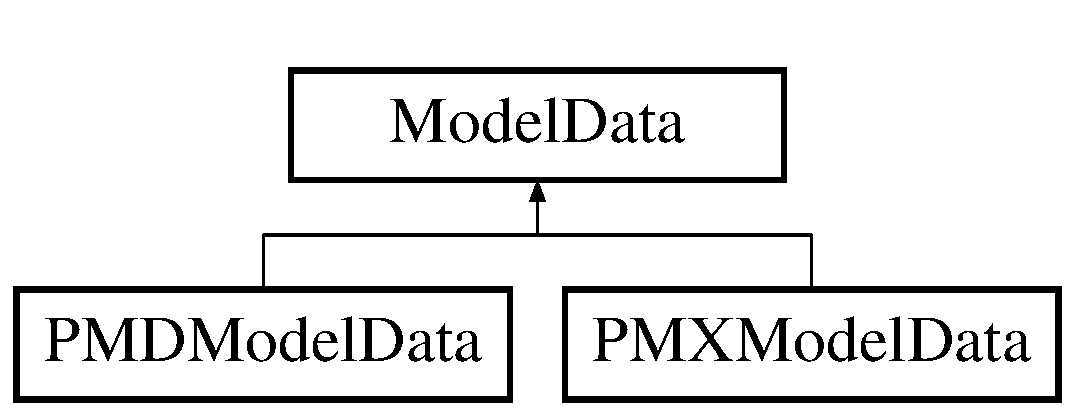
\includegraphics[height=2.000000cm]{class_model_data}
\end{center}
\end{figure}
\subsection*{公開メンバ関数}
\begin{DoxyCompactItemize}
\item 
\mbox{\hyperlink{class_model_data_a020b20ee652b493d6400f153cce4d391}{Model\+Data}} (std\+::shared\+\_\+ptr$<$ \mbox{\hyperlink{class_vertex_buffer}{Vertex\+Buffer}} $>$ vertex\+Buffer, std\+::shared\+\_\+ptr$<$ \mbox{\hyperlink{class_index_buffer}{Index\+Buffer}} $>$ index\+Buffer, std\+::shared\+\_\+ptr$<$ \mbox{\hyperlink{class_descriptor_heap}{Descriptor\+Heap}} $>$ descriptor\+Heap)
\begin{DoxyCompactList}\small\item\em コンストラクタ \end{DoxyCompactList}\item 
virtual \mbox{\hyperlink{class_model_data_a8888ea03c5d27446f2f7f93f6fe6cd42}{$\sim$\+Model\+Data}} ()
\begin{DoxyCompactList}\small\item\em デストラクタ \end{DoxyCompactList}\item 
std\+::shared\+\_\+ptr$<$ \mbox{\hyperlink{class_vertex_buffer}{Vertex\+Buffer}} $>$ \mbox{\hyperlink{class_model_data_a4c76f184b373d682cd94a21440730ac0}{Get\+Vertex\+Buffer}} () const
\begin{DoxyCompactList}\small\item\em 頂点バッファを取得する \end{DoxyCompactList}\item 
std\+::shared\+\_\+ptr$<$ \mbox{\hyperlink{class_index_buffer}{Index\+Buffer}} $>$ \mbox{\hyperlink{class_model_data_a4b0d36d5d77479dc7d08977aded2bc94}{Get\+Index\+Buffer}} () const
\begin{DoxyCompactList}\small\item\em インデックスバッファを取得する \end{DoxyCompactList}\item 
std\+::shared\+\_\+ptr$<$ \mbox{\hyperlink{class_descriptor_heap}{Descriptor\+Heap}} $>$ \mbox{\hyperlink{class_model_data_a7b30fc0bbceb348a615241b4fd333515}{Get\+Descriptor\+Heap}} () const
\begin{DoxyCompactList}\small\item\em デスクリプタヒープを取得する \end{DoxyCompactList}\item 
std\+::shared\+\_\+ptr$<$ \mbox{\hyperlink{class_pose}{Pose}} $>$ \mbox{\hyperlink{class_model_data_a7c43dc81e963e445250c2ae8aceae9d0}{\+\_\+\+Debug\+Get\+Pose}} () const
\item 
virtual void \mbox{\hyperlink{class_model_data_a67a18789221798611c63fd18edb3a9fc}{Update}} ()
\begin{DoxyCompactList}\small\item\em 更新処理 \end{DoxyCompactList}\item 
virtual void \mbox{\hyperlink{class_model_data_a774032c8dac7355ad2657c83cf0d1e21}{Draw}} (Com\+Ptr$<$ I\+D3\+D12\+Graphics\+Command\+List $>$ graphics\+Command\+List, const \mbox{\hyperlink{struct_instance_data}{Instance\+Data}} \&instance\+Data) const
\begin{DoxyCompactList}\small\item\em 描画処理 \end{DoxyCompactList}\end{DoxyCompactItemize}
\subsection*{限定公開変数類}
\begin{DoxyCompactItemize}
\item 
std\+::shared\+\_\+ptr$<$ \mbox{\hyperlink{class_vertex_buffer}{Vertex\+Buffer}} $>$ \mbox{\hyperlink{class_model_data_a5aa8473c9a0c82fcf9358e58a46d2ee0}{m\+Vertex\+Buffer}}
\item 
std\+::shared\+\_\+ptr$<$ \mbox{\hyperlink{class_index_buffer}{Index\+Buffer}} $>$ \mbox{\hyperlink{class_model_data_a62f3a9436dd4933a240ebb59a03f84bb}{m\+Index\+Buffer}}
\item 
std\+::shared\+\_\+ptr$<$ \mbox{\hyperlink{class_descriptor_heap}{Descriptor\+Heap}} $>$ \mbox{\hyperlink{class_model_data_aba1b9420b9caed0552c28bffd0914225}{m\+Desc\+Heap}}
\item 
std\+::shared\+\_\+ptr$<$ \mbox{\hyperlink{class_pose}{Pose}} $>$ \mbox{\hyperlink{class_model_data_a5136f7dc8b351f859681f6222d8c41c1}{m\+Pose}}
\end{DoxyCompactItemize}


\subsection{構築子と解体子}
\mbox{\Hypertarget{class_model_data_a020b20ee652b493d6400f153cce4d391}\label{class_model_data_a020b20ee652b493d6400f153cce4d391}} 
\index{Model\+Data@{Model\+Data}!Model\+Data@{Model\+Data}}
\index{Model\+Data@{Model\+Data}!Model\+Data@{Model\+Data}}
\subsubsection{\texorpdfstring{Model\+Data()}{ModelData()}}
{\footnotesize\ttfamily Model\+Data\+::\+Model\+Data (\begin{DoxyParamCaption}\item[{std\+::shared\+\_\+ptr$<$ \mbox{\hyperlink{class_vertex_buffer}{Vertex\+Buffer}} $>$}]{vertex\+Buffer,  }\item[{std\+::shared\+\_\+ptr$<$ \mbox{\hyperlink{class_index_buffer}{Index\+Buffer}} $>$}]{index\+Buffer,  }\item[{std\+::shared\+\_\+ptr$<$ \mbox{\hyperlink{class_descriptor_heap}{Descriptor\+Heap}} $>$}]{descriptor\+Heap }\end{DoxyParamCaption})}



コンストラクタ 

\mbox{\Hypertarget{class_model_data_a8888ea03c5d27446f2f7f93f6fe6cd42}\label{class_model_data_a8888ea03c5d27446f2f7f93f6fe6cd42}} 
\index{Model\+Data@{Model\+Data}!````~Model\+Data@{$\sim$\+Model\+Data}}
\index{````~Model\+Data@{$\sim$\+Model\+Data}!Model\+Data@{Model\+Data}}
\subsubsection{\texorpdfstring{$\sim$\+Model\+Data()}{~ModelData()}}
{\footnotesize\ttfamily Model\+Data\+::$\sim$\+Model\+Data (\begin{DoxyParamCaption}{ }\end{DoxyParamCaption})\hspace{0.3cm}{\ttfamily [virtual]}}



デストラクタ 



\subsection{関数詳解}
\mbox{\Hypertarget{class_model_data_a7c43dc81e963e445250c2ae8aceae9d0}\label{class_model_data_a7c43dc81e963e445250c2ae8aceae9d0}} 
\index{Model\+Data@{Model\+Data}!\+\_\+\+Debug\+Get\+Pose@{\+\_\+\+Debug\+Get\+Pose}}
\index{\+\_\+\+Debug\+Get\+Pose@{\+\_\+\+Debug\+Get\+Pose}!Model\+Data@{Model\+Data}}
\subsubsection{\texorpdfstring{\+\_\+\+Debug\+Get\+Pose()}{\_DebugGetPose()}}
{\footnotesize\ttfamily std\+::shared\+\_\+ptr$<$ \mbox{\hyperlink{class_pose}{Pose}} $>$ Model\+Data\+::\+\_\+\+Debug\+Get\+Pose (\begin{DoxyParamCaption}{ }\end{DoxyParamCaption}) const}

Debug 姿勢情報を取得する \mbox{\Hypertarget{class_model_data_a774032c8dac7355ad2657c83cf0d1e21}\label{class_model_data_a774032c8dac7355ad2657c83cf0d1e21}} 
\index{Model\+Data@{Model\+Data}!Draw@{Draw}}
\index{Draw@{Draw}!Model\+Data@{Model\+Data}}
\subsubsection{\texorpdfstring{Draw()}{Draw()}}
{\footnotesize\ttfamily void Model\+Data\+::\+Draw (\begin{DoxyParamCaption}\item[{Com\+Ptr$<$ I\+D3\+D12\+Graphics\+Command\+List $>$}]{graphics\+Command\+List,  }\item[{const \mbox{\hyperlink{struct_instance_data}{Instance\+Data}} \&}]{instance\+Data }\end{DoxyParamCaption}) const\hspace{0.3cm}{\ttfamily [virtual]}}



描画処理 



\mbox{\hyperlink{class_p_m_d_model_data_ae811d49854ae659f20ac9be60a5fb146}{P\+M\+D\+Model\+Data}}, \mbox{\hyperlink{class_p_m_x_model_data_aa88713736e3c337cabb23127c03be3c2}{P\+M\+X\+Model\+Data}}で再実装されています。

\mbox{\Hypertarget{class_model_data_a7b30fc0bbceb348a615241b4fd333515}\label{class_model_data_a7b30fc0bbceb348a615241b4fd333515}} 
\index{Model\+Data@{Model\+Data}!Get\+Descriptor\+Heap@{Get\+Descriptor\+Heap}}
\index{Get\+Descriptor\+Heap@{Get\+Descriptor\+Heap}!Model\+Data@{Model\+Data}}
\subsubsection{\texorpdfstring{Get\+Descriptor\+Heap()}{GetDescriptorHeap()}}
{\footnotesize\ttfamily std\+::shared\+\_\+ptr$<$ \mbox{\hyperlink{class_descriptor_heap}{Descriptor\+Heap}} $>$ Model\+Data\+::\+Get\+Descriptor\+Heap (\begin{DoxyParamCaption}{ }\end{DoxyParamCaption}) const}



デスクリプタヒープを取得する 

\mbox{\Hypertarget{class_model_data_a4b0d36d5d77479dc7d08977aded2bc94}\label{class_model_data_a4b0d36d5d77479dc7d08977aded2bc94}} 
\index{Model\+Data@{Model\+Data}!Get\+Index\+Buffer@{Get\+Index\+Buffer}}
\index{Get\+Index\+Buffer@{Get\+Index\+Buffer}!Model\+Data@{Model\+Data}}
\subsubsection{\texorpdfstring{Get\+Index\+Buffer()}{GetIndexBuffer()}}
{\footnotesize\ttfamily std\+::shared\+\_\+ptr$<$ \mbox{\hyperlink{class_index_buffer}{Index\+Buffer}} $>$ Model\+Data\+::\+Get\+Index\+Buffer (\begin{DoxyParamCaption}{ }\end{DoxyParamCaption}) const}



インデックスバッファを取得する 

\mbox{\Hypertarget{class_model_data_a4c76f184b373d682cd94a21440730ac0}\label{class_model_data_a4c76f184b373d682cd94a21440730ac0}} 
\index{Model\+Data@{Model\+Data}!Get\+Vertex\+Buffer@{Get\+Vertex\+Buffer}}
\index{Get\+Vertex\+Buffer@{Get\+Vertex\+Buffer}!Model\+Data@{Model\+Data}}
\subsubsection{\texorpdfstring{Get\+Vertex\+Buffer()}{GetVertexBuffer()}}
{\footnotesize\ttfamily std\+::shared\+\_\+ptr$<$ \mbox{\hyperlink{class_vertex_buffer}{Vertex\+Buffer}} $>$ Model\+Data\+::\+Get\+Vertex\+Buffer (\begin{DoxyParamCaption}{ }\end{DoxyParamCaption}) const}



頂点バッファを取得する 

\mbox{\Hypertarget{class_model_data_a67a18789221798611c63fd18edb3a9fc}\label{class_model_data_a67a18789221798611c63fd18edb3a9fc}} 
\index{Model\+Data@{Model\+Data}!Update@{Update}}
\index{Update@{Update}!Model\+Data@{Model\+Data}}
\subsubsection{\texorpdfstring{Update()}{Update()}}
{\footnotesize\ttfamily void Model\+Data\+::\+Update (\begin{DoxyParamCaption}{ }\end{DoxyParamCaption})\hspace{0.3cm}{\ttfamily [virtual]}}



更新処理 



\mbox{\hyperlink{class_p_m_x_model_data_a4c692007e0b890ee0bfd0f2bbbe0b97f}{P\+M\+X\+Model\+Data}}で再実装されています。



\subsection{メンバ詳解}
\mbox{\Hypertarget{class_model_data_aba1b9420b9caed0552c28bffd0914225}\label{class_model_data_aba1b9420b9caed0552c28bffd0914225}} 
\index{Model\+Data@{Model\+Data}!m\+Desc\+Heap@{m\+Desc\+Heap}}
\index{m\+Desc\+Heap@{m\+Desc\+Heap}!Model\+Data@{Model\+Data}}
\subsubsection{\texorpdfstring{m\+Desc\+Heap}{mDescHeap}}
{\footnotesize\ttfamily std\+::shared\+\_\+ptr$<$\mbox{\hyperlink{class_descriptor_heap}{Descriptor\+Heap}}$>$ Model\+Data\+::m\+Desc\+Heap\hspace{0.3cm}{\ttfamily [protected]}}

\mbox{\Hypertarget{class_model_data_a62f3a9436dd4933a240ebb59a03f84bb}\label{class_model_data_a62f3a9436dd4933a240ebb59a03f84bb}} 
\index{Model\+Data@{Model\+Data}!m\+Index\+Buffer@{m\+Index\+Buffer}}
\index{m\+Index\+Buffer@{m\+Index\+Buffer}!Model\+Data@{Model\+Data}}
\subsubsection{\texorpdfstring{m\+Index\+Buffer}{mIndexBuffer}}
{\footnotesize\ttfamily std\+::shared\+\_\+ptr$<$\mbox{\hyperlink{class_index_buffer}{Index\+Buffer}}$>$ Model\+Data\+::m\+Index\+Buffer\hspace{0.3cm}{\ttfamily [protected]}}

\mbox{\Hypertarget{class_model_data_a5136f7dc8b351f859681f6222d8c41c1}\label{class_model_data_a5136f7dc8b351f859681f6222d8c41c1}} 
\index{Model\+Data@{Model\+Data}!m\+Pose@{m\+Pose}}
\index{m\+Pose@{m\+Pose}!Model\+Data@{Model\+Data}}
\subsubsection{\texorpdfstring{m\+Pose}{mPose}}
{\footnotesize\ttfamily std\+::shared\+\_\+ptr$<$\mbox{\hyperlink{class_pose}{Pose}}$>$ Model\+Data\+::m\+Pose\hspace{0.3cm}{\ttfamily [protected]}}

\mbox{\Hypertarget{class_model_data_a5aa8473c9a0c82fcf9358e58a46d2ee0}\label{class_model_data_a5aa8473c9a0c82fcf9358e58a46d2ee0}} 
\index{Model\+Data@{Model\+Data}!m\+Vertex\+Buffer@{m\+Vertex\+Buffer}}
\index{m\+Vertex\+Buffer@{m\+Vertex\+Buffer}!Model\+Data@{Model\+Data}}
\subsubsection{\texorpdfstring{m\+Vertex\+Buffer}{mVertexBuffer}}
{\footnotesize\ttfamily std\+::shared\+\_\+ptr$<$\mbox{\hyperlink{class_vertex_buffer}{Vertex\+Buffer}}$>$ Model\+Data\+::m\+Vertex\+Buffer\hspace{0.3cm}{\ttfamily [protected]}}



このクラス詳解は次のファイルから抽出されました\+:\begin{DoxyCompactItemize}
\item 
Source/\+Model/\mbox{\hyperlink{_model_data_8h}{Model\+Data.\+h}}\item 
Source/\+Model/\mbox{\hyperlink{_model_data_8cpp}{Model\+Data.\+cpp}}\end{DoxyCompactItemize}

\hypertarget{struct_p_m_x_1_1_model_data_desc}{}\section{P\+MX\+:\+:Model\+Data\+Desc 構造体}
\label{struct_p_m_x_1_1_model_data_desc}\index{P\+M\+X\+::\+Model\+Data\+Desc@{P\+M\+X\+::\+Model\+Data\+Desc}}


{\ttfamily \#include $<$P\+M\+X\+Model\+Data\+Info.\+h$>$}

\subsection*{公開変数類}
\begin{DoxyCompactItemize}
\item 
std\+::wstring \mbox{\hyperlink{struct_p_m_x_1_1_model_data_desc_a68efc3cf4008e7ad21e1f8d3358fdee5}{model\+File\+Path}}
\item 
\mbox{\hyperlink{struct_p_m_x_1_1_header}{Header}} \mbox{\hyperlink{struct_p_m_x_1_1_model_data_desc_a1ead04540b79398f2ae7853298146830}{header}}
\item 
\mbox{\hyperlink{struct_p_m_x_1_1_model_info}{Model\+Info}} \mbox{\hyperlink{struct_p_m_x_1_1_model_data_desc_a1061040937cef4cfcbbf88e18ef213bf}{model\+Info}}
\item 
std\+::vector$<$ \mbox{\hyperlink{struct_p_m_x_1_1_vertex}{Vertex}} $>$ \mbox{\hyperlink{struct_p_m_x_1_1_model_data_desc_aa8ec22a2e7921bc95e7cd0435cccd22a}{vertices}}
\item 
std\+::vector$<$ \mbox{\hyperlink{struct_p_m_x_1_1_index}{Index}} $>$ \mbox{\hyperlink{struct_p_m_x_1_1_model_data_desc_ad9aab045cc87255e7d81b982ae4c3adb}{indexies}}
\item 
std\+::vector$<$ \mbox{\hyperlink{struct_p_m_x_1_1_texture}{P\+M\+X\+::\+Texture}} $>$ \mbox{\hyperlink{struct_p_m_x_1_1_model_data_desc_ac937446386ac6c0551c67e01c81d5b5f}{textures}}
\item 
std\+::vector$<$ \mbox{\hyperlink{struct_p_m_x_1_1_material}{Material}} $>$ \mbox{\hyperlink{struct_p_m_x_1_1_model_data_desc_a1e8286c2df43aef64cadffc581cf32de}{materials}}
\item 
std\+::vector$<$ \mbox{\hyperlink{struct_p_m_x_1_1_bone_data}{Bone\+Data}} $>$ \mbox{\hyperlink{struct_p_m_x_1_1_model_data_desc_a05537dc8d57924b4d524dc313f6dae2e}{bones}}
\item 
std\+::vector$<$ \mbox{\hyperlink{struct_p_m_x_1_1_morph}{Morph}} $>$ \mbox{\hyperlink{struct_p_m_x_1_1_model_data_desc_ac86acd041473edf937debb8c7a8afdb7}{morphs}}
\item 
std\+::vector$<$ \mbox{\hyperlink{struct_p_m_x_1_1_display_frame}{Display\+Frame}} $>$ \mbox{\hyperlink{struct_p_m_x_1_1_model_data_desc_a0ba429d52fd5b63bb11b7c89dd1787cf}{display\+Frame}}
\item 
std\+::vector$<$ \mbox{\hyperlink{struct_p_m_x_1_1_rigid_body}{Rigid\+Body}} $>$ \mbox{\hyperlink{struct_p_m_x_1_1_model_data_desc_acaf47c6a725110c90e3a59f5089b03d7}{rigid\+Bodies}}
\item 
std\+::vector$<$ \mbox{\hyperlink{struct_p_m_x_1_1_joint}{Joint}} $>$ \mbox{\hyperlink{struct_p_m_x_1_1_model_data_desc_ae5e3126a09a5d036046f534f290408cd}{joints}}
\end{DoxyCompactItemize}


\subsection{メンバ詳解}
\mbox{\Hypertarget{struct_p_m_x_1_1_model_data_desc_a05537dc8d57924b4d524dc313f6dae2e}\label{struct_p_m_x_1_1_model_data_desc_a05537dc8d57924b4d524dc313f6dae2e}} 
\index{P\+M\+X\+::\+Model\+Data\+Desc@{P\+M\+X\+::\+Model\+Data\+Desc}!bones@{bones}}
\index{bones@{bones}!P\+M\+X\+::\+Model\+Data\+Desc@{P\+M\+X\+::\+Model\+Data\+Desc}}
\subsubsection{\texorpdfstring{bones}{bones}}
{\footnotesize\ttfamily std\+::vector$<$\mbox{\hyperlink{struct_p_m_x_1_1_bone_data}{Bone\+Data}}$>$ P\+M\+X\+::\+Model\+Data\+Desc\+::bones}

\mbox{\Hypertarget{struct_p_m_x_1_1_model_data_desc_a0ba429d52fd5b63bb11b7c89dd1787cf}\label{struct_p_m_x_1_1_model_data_desc_a0ba429d52fd5b63bb11b7c89dd1787cf}} 
\index{P\+M\+X\+::\+Model\+Data\+Desc@{P\+M\+X\+::\+Model\+Data\+Desc}!display\+Frame@{display\+Frame}}
\index{display\+Frame@{display\+Frame}!P\+M\+X\+::\+Model\+Data\+Desc@{P\+M\+X\+::\+Model\+Data\+Desc}}
\subsubsection{\texorpdfstring{display\+Frame}{displayFrame}}
{\footnotesize\ttfamily std\+::vector$<$\mbox{\hyperlink{struct_p_m_x_1_1_display_frame}{Display\+Frame}}$>$ P\+M\+X\+::\+Model\+Data\+Desc\+::display\+Frame}

\mbox{\Hypertarget{struct_p_m_x_1_1_model_data_desc_a1ead04540b79398f2ae7853298146830}\label{struct_p_m_x_1_1_model_data_desc_a1ead04540b79398f2ae7853298146830}} 
\index{P\+M\+X\+::\+Model\+Data\+Desc@{P\+M\+X\+::\+Model\+Data\+Desc}!header@{header}}
\index{header@{header}!P\+M\+X\+::\+Model\+Data\+Desc@{P\+M\+X\+::\+Model\+Data\+Desc}}
\subsubsection{\texorpdfstring{header}{header}}
{\footnotesize\ttfamily \mbox{\hyperlink{struct_p_m_x_1_1_header}{Header}} P\+M\+X\+::\+Model\+Data\+Desc\+::header}

\mbox{\Hypertarget{struct_p_m_x_1_1_model_data_desc_ad9aab045cc87255e7d81b982ae4c3adb}\label{struct_p_m_x_1_1_model_data_desc_ad9aab045cc87255e7d81b982ae4c3adb}} 
\index{P\+M\+X\+::\+Model\+Data\+Desc@{P\+M\+X\+::\+Model\+Data\+Desc}!indexies@{indexies}}
\index{indexies@{indexies}!P\+M\+X\+::\+Model\+Data\+Desc@{P\+M\+X\+::\+Model\+Data\+Desc}}
\subsubsection{\texorpdfstring{indexies}{indexies}}
{\footnotesize\ttfamily std\+::vector$<$\mbox{\hyperlink{struct_p_m_x_1_1_index}{Index}}$>$ P\+M\+X\+::\+Model\+Data\+Desc\+::indexies}

\mbox{\Hypertarget{struct_p_m_x_1_1_model_data_desc_ae5e3126a09a5d036046f534f290408cd}\label{struct_p_m_x_1_1_model_data_desc_ae5e3126a09a5d036046f534f290408cd}} 
\index{P\+M\+X\+::\+Model\+Data\+Desc@{P\+M\+X\+::\+Model\+Data\+Desc}!joints@{joints}}
\index{joints@{joints}!P\+M\+X\+::\+Model\+Data\+Desc@{P\+M\+X\+::\+Model\+Data\+Desc}}
\subsubsection{\texorpdfstring{joints}{joints}}
{\footnotesize\ttfamily std\+::vector$<$\mbox{\hyperlink{struct_p_m_x_1_1_joint}{Joint}}$>$ P\+M\+X\+::\+Model\+Data\+Desc\+::joints}

\mbox{\Hypertarget{struct_p_m_x_1_1_model_data_desc_a1e8286c2df43aef64cadffc581cf32de}\label{struct_p_m_x_1_1_model_data_desc_a1e8286c2df43aef64cadffc581cf32de}} 
\index{P\+M\+X\+::\+Model\+Data\+Desc@{P\+M\+X\+::\+Model\+Data\+Desc}!materials@{materials}}
\index{materials@{materials}!P\+M\+X\+::\+Model\+Data\+Desc@{P\+M\+X\+::\+Model\+Data\+Desc}}
\subsubsection{\texorpdfstring{materials}{materials}}
{\footnotesize\ttfamily std\+::vector$<$\mbox{\hyperlink{struct_p_m_x_1_1_material}{Material}}$>$ P\+M\+X\+::\+Model\+Data\+Desc\+::materials}

\mbox{\Hypertarget{struct_p_m_x_1_1_model_data_desc_a68efc3cf4008e7ad21e1f8d3358fdee5}\label{struct_p_m_x_1_1_model_data_desc_a68efc3cf4008e7ad21e1f8d3358fdee5}} 
\index{P\+M\+X\+::\+Model\+Data\+Desc@{P\+M\+X\+::\+Model\+Data\+Desc}!model\+File\+Path@{model\+File\+Path}}
\index{model\+File\+Path@{model\+File\+Path}!P\+M\+X\+::\+Model\+Data\+Desc@{P\+M\+X\+::\+Model\+Data\+Desc}}
\subsubsection{\texorpdfstring{model\+File\+Path}{modelFilePath}}
{\footnotesize\ttfamily std\+::wstring P\+M\+X\+::\+Model\+Data\+Desc\+::model\+File\+Path}

\mbox{\Hypertarget{struct_p_m_x_1_1_model_data_desc_a1061040937cef4cfcbbf88e18ef213bf}\label{struct_p_m_x_1_1_model_data_desc_a1061040937cef4cfcbbf88e18ef213bf}} 
\index{P\+M\+X\+::\+Model\+Data\+Desc@{P\+M\+X\+::\+Model\+Data\+Desc}!model\+Info@{model\+Info}}
\index{model\+Info@{model\+Info}!P\+M\+X\+::\+Model\+Data\+Desc@{P\+M\+X\+::\+Model\+Data\+Desc}}
\subsubsection{\texorpdfstring{model\+Info}{modelInfo}}
{\footnotesize\ttfamily \mbox{\hyperlink{struct_p_m_x_1_1_model_info}{Model\+Info}} P\+M\+X\+::\+Model\+Data\+Desc\+::model\+Info}

\mbox{\Hypertarget{struct_p_m_x_1_1_model_data_desc_ac86acd041473edf937debb8c7a8afdb7}\label{struct_p_m_x_1_1_model_data_desc_ac86acd041473edf937debb8c7a8afdb7}} 
\index{P\+M\+X\+::\+Model\+Data\+Desc@{P\+M\+X\+::\+Model\+Data\+Desc}!morphs@{morphs}}
\index{morphs@{morphs}!P\+M\+X\+::\+Model\+Data\+Desc@{P\+M\+X\+::\+Model\+Data\+Desc}}
\subsubsection{\texorpdfstring{morphs}{morphs}}
{\footnotesize\ttfamily std\+::vector$<$\mbox{\hyperlink{struct_p_m_x_1_1_morph}{Morph}}$>$ P\+M\+X\+::\+Model\+Data\+Desc\+::morphs}

\mbox{\Hypertarget{struct_p_m_x_1_1_model_data_desc_acaf47c6a725110c90e3a59f5089b03d7}\label{struct_p_m_x_1_1_model_data_desc_acaf47c6a725110c90e3a59f5089b03d7}} 
\index{P\+M\+X\+::\+Model\+Data\+Desc@{P\+M\+X\+::\+Model\+Data\+Desc}!rigid\+Bodies@{rigid\+Bodies}}
\index{rigid\+Bodies@{rigid\+Bodies}!P\+M\+X\+::\+Model\+Data\+Desc@{P\+M\+X\+::\+Model\+Data\+Desc}}
\subsubsection{\texorpdfstring{rigid\+Bodies}{rigidBodies}}
{\footnotesize\ttfamily std\+::vector$<$\mbox{\hyperlink{struct_p_m_x_1_1_rigid_body}{Rigid\+Body}}$>$ P\+M\+X\+::\+Model\+Data\+Desc\+::rigid\+Bodies}

\mbox{\Hypertarget{struct_p_m_x_1_1_model_data_desc_ac937446386ac6c0551c67e01c81d5b5f}\label{struct_p_m_x_1_1_model_data_desc_ac937446386ac6c0551c67e01c81d5b5f}} 
\index{P\+M\+X\+::\+Model\+Data\+Desc@{P\+M\+X\+::\+Model\+Data\+Desc}!textures@{textures}}
\index{textures@{textures}!P\+M\+X\+::\+Model\+Data\+Desc@{P\+M\+X\+::\+Model\+Data\+Desc}}
\subsubsection{\texorpdfstring{textures}{textures}}
{\footnotesize\ttfamily std\+::vector$<$\mbox{\hyperlink{struct_p_m_x_1_1_texture}{P\+M\+X\+::\+Texture}}$>$ P\+M\+X\+::\+Model\+Data\+Desc\+::textures}

\mbox{\Hypertarget{struct_p_m_x_1_1_model_data_desc_aa8ec22a2e7921bc95e7cd0435cccd22a}\label{struct_p_m_x_1_1_model_data_desc_aa8ec22a2e7921bc95e7cd0435cccd22a}} 
\index{P\+M\+X\+::\+Model\+Data\+Desc@{P\+M\+X\+::\+Model\+Data\+Desc}!vertices@{vertices}}
\index{vertices@{vertices}!P\+M\+X\+::\+Model\+Data\+Desc@{P\+M\+X\+::\+Model\+Data\+Desc}}
\subsubsection{\texorpdfstring{vertices}{vertices}}
{\footnotesize\ttfamily std\+::vector$<$\mbox{\hyperlink{struct_p_m_x_1_1_vertex}{Vertex}}$>$ P\+M\+X\+::\+Model\+Data\+Desc\+::vertices}



この構造体詳解は次のファイルから抽出されました\+:\begin{DoxyCompactItemize}
\item 
Source/\mbox{\hyperlink{_p_m_x_model_data_info_8h}{P\+M\+X\+Model\+Data\+Info.\+h}}\end{DoxyCompactItemize}

\hypertarget{class_model_data_manager}{}\section{Model\+Data\+Manager クラス}
\label{class_model_data_manager}\index{Model\+Data\+Manager@{Model\+Data\+Manager}}


{\ttfamily \#include $<$Model\+Data\+Manager.\+h$>$}

\subsection*{公開メンバ関数}
\begin{DoxyCompactItemize}
\item 
\mbox{\hyperlink{class_model_data_manager_ad8a24b96d273af9e717e7cc4b68cf399}{$\sim$\+Model\+Data\+Manager}} ()
\item 
int \mbox{\hyperlink{class_model_data_manager_a20b9312e019c39c633d6429e1209d1b7}{Regist}} (std\+::shared\+\_\+ptr$<$ \mbox{\hyperlink{class_model_data}{Model\+Data}} $>$ model\+Data)
\item 
void \mbox{\hyperlink{class_model_data_manager_aaa1dc0669900e8dc8186ae075133ba24}{Erase}} (int handle)
\item 
std\+::shared\+\_\+ptr$<$ \mbox{\hyperlink{class_model_data}{Model\+Data}} $>$ \mbox{\hyperlink{class_model_data_manager_a5f823590ae9c9eac222a7b107d14634b}{Get\+Model\+Data}} (int handle) const
\item 
bool \mbox{\hyperlink{class_model_data_manager_a69c14318f17547e1145b714a613732bc}{Is\+Exist}} (int handle) const
\item 
void \mbox{\hyperlink{class_model_data_manager_a9c2d9c3a70323f7d486fb42de162d303}{Draw}} (Com\+Ptr$<$ I\+D3\+D12\+Graphics\+Command\+List $>$ graphics\+Command\+List)
\end{DoxyCompactItemize}
\subsection*{静的公開メンバ関数}
\begin{DoxyCompactItemize}
\item 
static \mbox{\hyperlink{class_model_data_manager}{Model\+Data\+Manager}} \& \mbox{\hyperlink{class_model_data_manager_aee0cb9bcad096186bd2902620d1ac780}{Get\+Instance}} ()
\end{DoxyCompactItemize}


\subsection{構築子と解体子}
\mbox{\Hypertarget{class_model_data_manager_ad8a24b96d273af9e717e7cc4b68cf399}\label{class_model_data_manager_ad8a24b96d273af9e717e7cc4b68cf399}} 
\index{Model\+Data\+Manager@{Model\+Data\+Manager}!````~Model\+Data\+Manager@{$\sim$\+Model\+Data\+Manager}}
\index{````~Model\+Data\+Manager@{$\sim$\+Model\+Data\+Manager}!Model\+Data\+Manager@{Model\+Data\+Manager}}
\subsubsection{\texorpdfstring{$\sim$\+Model\+Data\+Manager()}{~ModelDataManager()}}
{\footnotesize\ttfamily Model\+Data\+Manager\+::$\sim$\+Model\+Data\+Manager (\begin{DoxyParamCaption}{ }\end{DoxyParamCaption})}



\subsection{関数詳解}
\mbox{\Hypertarget{class_model_data_manager_a9c2d9c3a70323f7d486fb42de162d303}\label{class_model_data_manager_a9c2d9c3a70323f7d486fb42de162d303}} 
\index{Model\+Data\+Manager@{Model\+Data\+Manager}!Draw@{Draw}}
\index{Draw@{Draw}!Model\+Data\+Manager@{Model\+Data\+Manager}}
\subsubsection{\texorpdfstring{Draw()}{Draw()}}
{\footnotesize\ttfamily Model\+Data\+Manager\+::\+Draw (\begin{DoxyParamCaption}\item[{Com\+Ptr$<$ I\+D3\+D12\+Graphics\+Command\+List $>$}]{graphics\+Command\+List }\end{DoxyParamCaption})}

管理しているモデルデータを描画する 
\begin{DoxyParams}[1]{引数}
\mbox{\tt in}  & {\em graphics\+Command\+List} & \+: 描画先コマンドリスト \\
\hline
\end{DoxyParams}
\mbox{\Hypertarget{class_model_data_manager_aaa1dc0669900e8dc8186ae075133ba24}\label{class_model_data_manager_aaa1dc0669900e8dc8186ae075133ba24}} 
\index{Model\+Data\+Manager@{Model\+Data\+Manager}!Erase@{Erase}}
\index{Erase@{Erase}!Model\+Data\+Manager@{Model\+Data\+Manager}}
\subsubsection{\texorpdfstring{Erase()}{Erase()}}
{\footnotesize\ttfamily Model\+Data\+Manager\+::\+Erase (\begin{DoxyParamCaption}\item[{int}]{handle }\end{DoxyParamCaption})}

指定したハンドルのモデルデータを削除する 
\begin{DoxyParams}[1]{引数}
\mbox{\tt in}  & {\em handle} & モデルハンドル \\
\hline
\end{DoxyParams}
\mbox{\Hypertarget{class_model_data_manager_aee0cb9bcad096186bd2902620d1ac780}\label{class_model_data_manager_aee0cb9bcad096186bd2902620d1ac780}} 
\index{Model\+Data\+Manager@{Model\+Data\+Manager}!Get\+Instance@{Get\+Instance}}
\index{Get\+Instance@{Get\+Instance}!Model\+Data\+Manager@{Model\+Data\+Manager}}
\subsubsection{\texorpdfstring{Get\+Instance()}{GetInstance()}}
{\footnotesize\ttfamily static Model\+Data\+Manager\+::\+Get\+Instance (\begin{DoxyParamCaption}{ }\end{DoxyParamCaption})\hspace{0.3cm}{\ttfamily [inline]}, {\ttfamily [static]}}

シングルトンインスタンスを取得する 
\begin{DoxyRetVals}{戻り値}
{\em モデルマネージャのインスタンス} & \\
\hline
\end{DoxyRetVals}
\mbox{\Hypertarget{class_model_data_manager_a5f823590ae9c9eac222a7b107d14634b}\label{class_model_data_manager_a5f823590ae9c9eac222a7b107d14634b}} 
\index{Model\+Data\+Manager@{Model\+Data\+Manager}!Get\+Model\+Data@{Get\+Model\+Data}}
\index{Get\+Model\+Data@{Get\+Model\+Data}!Model\+Data\+Manager@{Model\+Data\+Manager}}
\subsubsection{\texorpdfstring{Get\+Model\+Data()}{GetModelData()}}
{\footnotesize\ttfamily Model\+Data\+Manager\+::\+Get\+Model\+Data (\begin{DoxyParamCaption}\item[{int}]{handle }\end{DoxyParamCaption}) const}

モデルデータを作成する 
\begin{DoxyParams}[1]{引数}
\mbox{\tt in}  & {\em handle} & \+: モデルハンドル \\
\hline
\end{DoxyParams}

\begin{DoxyRetVals}{戻り値}
{\em モデルデータ} & \\
\hline
\end{DoxyRetVals}
\mbox{\Hypertarget{class_model_data_manager_a69c14318f17547e1145b714a613732bc}\label{class_model_data_manager_a69c14318f17547e1145b714a613732bc}} 
\index{Model\+Data\+Manager@{Model\+Data\+Manager}!Is\+Exist@{Is\+Exist}}
\index{Is\+Exist@{Is\+Exist}!Model\+Data\+Manager@{Model\+Data\+Manager}}
\subsubsection{\texorpdfstring{Is\+Exist()}{IsExist()}}
{\footnotesize\ttfamily Model\+Data\+Manager\+::\+Is\+Exist (\begin{DoxyParamCaption}\item[{int}]{handle }\end{DoxyParamCaption}) const}

指定したハンドルを指すモデルデータが存在するが確認する 
\begin{DoxyParams}[1]{引数}
\mbox{\tt in}  & {\em handle} & \+: テクスチャハンドル \\
\hline
\end{DoxyParams}

\begin{DoxyRetVals}{戻り値}
{\em 存在する} & true \\
\hline
{\em 存在しない} & false \\
\hline
\end{DoxyRetVals}
\mbox{\Hypertarget{class_model_data_manager_a20b9312e019c39c633d6429e1209d1b7}\label{class_model_data_manager_a20b9312e019c39c633d6429e1209d1b7}} 
\index{Model\+Data\+Manager@{Model\+Data\+Manager}!Regist@{Regist}}
\index{Regist@{Regist}!Model\+Data\+Manager@{Model\+Data\+Manager}}
\subsubsection{\texorpdfstring{Regist()}{Regist()}}
{\footnotesize\ttfamily Model\+Data\+Manager\+::\+Regist (\begin{DoxyParamCaption}\item[{std\+::shared\+\_\+ptr$<$ \mbox{\hyperlink{class_model_data}{Model\+Data}} $>$}]{model\+Data }\end{DoxyParamCaption})}

モデルデータを登録し、管理ハンドルを返す 
\begin{DoxyParams}[1]{引数}
\mbox{\tt in}  & {\em model\+Data} & モデルデータ \\
\hline
\end{DoxyParams}

\begin{DoxyRetVals}{戻り値}
{\em モデルデータのハンドル} & \\
\hline
\end{DoxyRetVals}


このクラス詳解は次のファイルから抽出されました\+:\begin{DoxyCompactItemize}
\item 
Source/\+Model/\mbox{\hyperlink{_model_data_manager_8h}{Model\+Data\+Manager.\+h}}\item 
Source/\+Model/\mbox{\hyperlink{_model_data_manager_8cpp}{Model\+Data\+Manager.\+cpp}}\end{DoxyCompactItemize}

\hypertarget{struct_p_m_x_1_1_model_info}{}\section{P\+MX\+:\+:Model\+Info 構造体}
\label{struct_p_m_x_1_1_model_info}\index{P\+M\+X\+::\+Model\+Info@{P\+M\+X\+::\+Model\+Info}}


{\ttfamily \#include $<$P\+M\+X\+Model\+Data\+Info.\+h$>$}

\subsection*{公開変数類}
\begin{DoxyCompactItemize}
\item 
std\+::wstring \mbox{\hyperlink{struct_p_m_x_1_1_model_info_aef4b5c31db4a895d72c82d8e9f762037}{model\+Name}}
\item 
std\+::wstring \mbox{\hyperlink{struct_p_m_x_1_1_model_info_a39f11c83c092fe840ceef5ce466c003f}{model\+Name\+Eng}}
\item 
std\+::wstring \mbox{\hyperlink{struct_p_m_x_1_1_model_info_adf2493db6d2f467f1f71e91b148ba8a9}{comment}}
\item 
std\+::wstring \mbox{\hyperlink{struct_p_m_x_1_1_model_info_ae58370a2e85443fa2a60a90eacc92826}{comment\+Eng}}
\end{DoxyCompactItemize}


\subsection{メンバ詳解}
\mbox{\Hypertarget{struct_p_m_x_1_1_model_info_adf2493db6d2f467f1f71e91b148ba8a9}\label{struct_p_m_x_1_1_model_info_adf2493db6d2f467f1f71e91b148ba8a9}} 
\index{P\+M\+X\+::\+Model\+Info@{P\+M\+X\+::\+Model\+Info}!comment@{comment}}
\index{comment@{comment}!P\+M\+X\+::\+Model\+Info@{P\+M\+X\+::\+Model\+Info}}
\subsubsection{\texorpdfstring{comment}{comment}}
{\footnotesize\ttfamily std\+::wstring P\+M\+X\+::\+Model\+Info\+::comment}

\mbox{\Hypertarget{struct_p_m_x_1_1_model_info_ae58370a2e85443fa2a60a90eacc92826}\label{struct_p_m_x_1_1_model_info_ae58370a2e85443fa2a60a90eacc92826}} 
\index{P\+M\+X\+::\+Model\+Info@{P\+M\+X\+::\+Model\+Info}!comment\+Eng@{comment\+Eng}}
\index{comment\+Eng@{comment\+Eng}!P\+M\+X\+::\+Model\+Info@{P\+M\+X\+::\+Model\+Info}}
\subsubsection{\texorpdfstring{comment\+Eng}{commentEng}}
{\footnotesize\ttfamily std\+::wstring P\+M\+X\+::\+Model\+Info\+::comment\+Eng}

\mbox{\Hypertarget{struct_p_m_x_1_1_model_info_aef4b5c31db4a895d72c82d8e9f762037}\label{struct_p_m_x_1_1_model_info_aef4b5c31db4a895d72c82d8e9f762037}} 
\index{P\+M\+X\+::\+Model\+Info@{P\+M\+X\+::\+Model\+Info}!model\+Name@{model\+Name}}
\index{model\+Name@{model\+Name}!P\+M\+X\+::\+Model\+Info@{P\+M\+X\+::\+Model\+Info}}
\subsubsection{\texorpdfstring{model\+Name}{modelName}}
{\footnotesize\ttfamily std\+::wstring P\+M\+X\+::\+Model\+Info\+::model\+Name}

\mbox{\Hypertarget{struct_p_m_x_1_1_model_info_a39f11c83c092fe840ceef5ce466c003f}\label{struct_p_m_x_1_1_model_info_a39f11c83c092fe840ceef5ce466c003f}} 
\index{P\+M\+X\+::\+Model\+Info@{P\+M\+X\+::\+Model\+Info}!model\+Name\+Eng@{model\+Name\+Eng}}
\index{model\+Name\+Eng@{model\+Name\+Eng}!P\+M\+X\+::\+Model\+Info@{P\+M\+X\+::\+Model\+Info}}
\subsubsection{\texorpdfstring{model\+Name\+Eng}{modelNameEng}}
{\footnotesize\ttfamily std\+::wstring P\+M\+X\+::\+Model\+Info\+::model\+Name\+Eng}



この構造体詳解は次のファイルから抽出されました\+:\begin{DoxyCompactItemize}
\item 
Source/\mbox{\hyperlink{_p_m_x_model_data_info_8h}{P\+M\+X\+Model\+Data\+Info.\+h}}\end{DoxyCompactItemize}

\hypertarget{class_model_loader}{}\section{Model\+Loader クラス}
\label{class_model_loader}\index{Model\+Loader@{Model\+Loader}}


{\ttfamily \#include $<$Model\+Loader.\+h$>$}

Model\+Loader の継承関係図\begin{figure}[H]
\begin{center}
\leavevmode
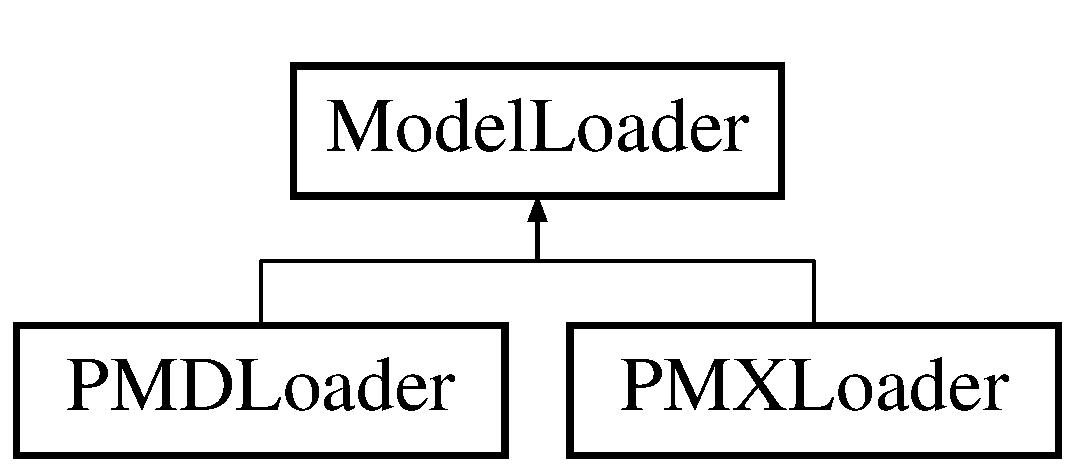
\includegraphics[height=2.000000cm]{class_model_loader}
\end{center}
\end{figure}
\subsection*{公開メンバ関数}
\begin{DoxyCompactItemize}
\item 
virtual \mbox{\hyperlink{class_model_loader_a4015291af96be2ea657577bdf4fb29f4}{$\sim$\+Model\+Loader}} ()
\begin{DoxyCompactList}\small\item\em デストラクタ \end{DoxyCompactList}\item 
virtual std\+::shared\+\_\+ptr$<$ \mbox{\hyperlink{class_model}{Model}} $>$ \mbox{\hyperlink{class_model_loader_a8e2157daa8d364c36fd26922f04adcb0}{Load\+Model}} (const std\+::string \&file\+Path)=0
\item 
virtual void \mbox{\hyperlink{class_model_loader_a6662edd78b17eeead09e822e19fc1799}{Clear\+Model\+Data}} ()=0
\end{DoxyCompactItemize}
\subsection*{限定公開メンバ関数}
\begin{DoxyCompactItemize}
\item 
\mbox{\hyperlink{class_model_loader_a0e7c5aa28d4772857b1bab0a9ca7428f}{Model\+Loader}} (std\+::shared\+\_\+ptr$<$ \mbox{\hyperlink{class_device}{Device}} $>$ device)
\begin{DoxyCompactList}\small\item\em コンストラクタ \end{DoxyCompactList}\end{DoxyCompactItemize}
\subsection*{限定公開変数類}
\begin{DoxyCompactItemize}
\item 
std\+::shared\+\_\+ptr$<$ \mbox{\hyperlink{class_device}{Device}} $>$ \mbox{\hyperlink{class_model_loader_a2e5b33970d8a71e5851e3b51b7980fa8}{m\+Device}}
\item 
\mbox{\hyperlink{class_model_data_manager}{Model\+Data\+Manager}} \& \mbox{\hyperlink{class_model_loader_a5877a5f2d2ec8db87cdcbf0a87c8587b}{m\+Model\+Data\+Manager}}
\item 
std\+::map$<$ std\+::string, int $>$ \mbox{\hyperlink{class_model_loader_a8d1002a30494635ec76972f3354f1ba9}{m\+Model\+Handle\+Manager}}
\end{DoxyCompactItemize}


\subsection{構築子と解体子}
\mbox{\Hypertarget{class_model_loader_a4015291af96be2ea657577bdf4fb29f4}\label{class_model_loader_a4015291af96be2ea657577bdf4fb29f4}} 
\index{Model\+Loader@{Model\+Loader}!````~Model\+Loader@{$\sim$\+Model\+Loader}}
\index{````~Model\+Loader@{$\sim$\+Model\+Loader}!Model\+Loader@{Model\+Loader}}
\subsubsection{\texorpdfstring{$\sim$\+Model\+Loader()}{~ModelLoader()}}
{\footnotesize\ttfamily Model\+Loader\+::$\sim$\+Model\+Loader (\begin{DoxyParamCaption}{ }\end{DoxyParamCaption})\hspace{0.3cm}{\ttfamily [virtual]}}



デストラクタ 

\mbox{\Hypertarget{class_model_loader_a0e7c5aa28d4772857b1bab0a9ca7428f}\label{class_model_loader_a0e7c5aa28d4772857b1bab0a9ca7428f}} 
\index{Model\+Loader@{Model\+Loader}!Model\+Loader@{Model\+Loader}}
\index{Model\+Loader@{Model\+Loader}!Model\+Loader@{Model\+Loader}}
\subsubsection{\texorpdfstring{Model\+Loader()}{ModelLoader()}}
{\footnotesize\ttfamily Model\+Loader\+::\+Model\+Loader (\begin{DoxyParamCaption}\item[{std\+::shared\+\_\+ptr$<$ \mbox{\hyperlink{class_device}{Device}} $>$}]{device }\end{DoxyParamCaption})\hspace{0.3cm}{\ttfamily [protected]}}



コンストラクタ 



\subsection{関数詳解}
\mbox{\Hypertarget{class_model_loader_a6662edd78b17eeead09e822e19fc1799}\label{class_model_loader_a6662edd78b17eeead09e822e19fc1799}} 
\index{Model\+Loader@{Model\+Loader}!Clear\+Model\+Data@{Clear\+Model\+Data}}
\index{Clear\+Model\+Data@{Clear\+Model\+Data}!Model\+Loader@{Model\+Loader}}
\subsubsection{\texorpdfstring{Clear\+Model\+Data()}{ClearModelData()}}
{\footnotesize\ttfamily Model\+Loader\+::\+Clear\+Model\+Data (\begin{DoxyParamCaption}{ }\end{DoxyParamCaption})\hspace{0.3cm}{\ttfamily [pure virtual]}}

読み込んだモデル情報を削除する 

\mbox{\hyperlink{class_p_m_x_loader_a1c4f3f379e18d6978b7684ab9d901952}{P\+M\+X\+Loader}}, \mbox{\hyperlink{class_p_m_d_loader_abdb6e537aef759341dfc62cd1038539c}{P\+M\+D\+Loader}}で実装されています。

\mbox{\Hypertarget{class_model_loader_a8e2157daa8d364c36fd26922f04adcb0}\label{class_model_loader_a8e2157daa8d364c36fd26922f04adcb0}} 
\index{Model\+Loader@{Model\+Loader}!Load\+Model@{Load\+Model}}
\index{Load\+Model@{Load\+Model}!Model\+Loader@{Model\+Loader}}
\subsubsection{\texorpdfstring{Load\+Model()}{LoadModel()}}
{\footnotesize\ttfamily Model\+Loader\+::\+Load\+Model (\begin{DoxyParamCaption}\item[{const std\+::string \&}]{file\+Path }\end{DoxyParamCaption})\hspace{0.3cm}{\ttfamily [pure virtual]}}

モデルをロードする 
\begin{DoxyParams}[1]{引数}
\mbox{\tt in}  & {\em file\+Path} & \+: ファイルパス \\
\hline
\end{DoxyParams}


\mbox{\hyperlink{class_p_m_x_loader_aee4e81ab65eeec5c9772ed5a8de6c5fa}{P\+M\+X\+Loader}}, \mbox{\hyperlink{class_p_m_d_loader_ae1da98c6236a58940ec521521e5c8288}{P\+M\+D\+Loader}}で実装されています。



\subsection{メンバ詳解}
\mbox{\Hypertarget{class_model_loader_a2e5b33970d8a71e5851e3b51b7980fa8}\label{class_model_loader_a2e5b33970d8a71e5851e3b51b7980fa8}} 
\index{Model\+Loader@{Model\+Loader}!m\+Device@{m\+Device}}
\index{m\+Device@{m\+Device}!Model\+Loader@{Model\+Loader}}
\subsubsection{\texorpdfstring{m\+Device}{mDevice}}
{\footnotesize\ttfamily std\+::shared\+\_\+ptr$<$\mbox{\hyperlink{class_device}{Device}}$>$ Model\+Loader\+::m\+Device\hspace{0.3cm}{\ttfamily [protected]}}

\mbox{\Hypertarget{class_model_loader_a5877a5f2d2ec8db87cdcbf0a87c8587b}\label{class_model_loader_a5877a5f2d2ec8db87cdcbf0a87c8587b}} 
\index{Model\+Loader@{Model\+Loader}!m\+Model\+Data\+Manager@{m\+Model\+Data\+Manager}}
\index{m\+Model\+Data\+Manager@{m\+Model\+Data\+Manager}!Model\+Loader@{Model\+Loader}}
\subsubsection{\texorpdfstring{m\+Model\+Data\+Manager}{mModelDataManager}}
{\footnotesize\ttfamily \mbox{\hyperlink{class_model_data_manager}{Model\+Data\+Manager}}\& Model\+Loader\+::m\+Model\+Data\+Manager\hspace{0.3cm}{\ttfamily [protected]}}

\mbox{\Hypertarget{class_model_loader_a8d1002a30494635ec76972f3354f1ba9}\label{class_model_loader_a8d1002a30494635ec76972f3354f1ba9}} 
\index{Model\+Loader@{Model\+Loader}!m\+Model\+Handle\+Manager@{m\+Model\+Handle\+Manager}}
\index{m\+Model\+Handle\+Manager@{m\+Model\+Handle\+Manager}!Model\+Loader@{Model\+Loader}}
\subsubsection{\texorpdfstring{m\+Model\+Handle\+Manager}{mModelHandleManager}}
{\footnotesize\ttfamily std\+::map$<$std\+::string, int$>$ Model\+Loader\+::m\+Model\+Handle\+Manager\hspace{0.3cm}{\ttfamily [protected]}}



このクラス詳解は次のファイルから抽出されました\+:\begin{DoxyCompactItemize}
\item 
Source/\+Model/\mbox{\hyperlink{_model_loader_8h}{Model\+Loader.\+h}}\item 
Source/\+Model/\mbox{\hyperlink{_model_loader_8cpp}{Model\+Loader.\+cpp}}\end{DoxyCompactItemize}

\hypertarget{struct_p_m_x_1_1_morph}{}\section{P\+MX\+:\+:Morph 構造体}
\label{struct_p_m_x_1_1_morph}\index{P\+M\+X\+::\+Morph@{P\+M\+X\+::\+Morph}}


{\ttfamily \#include $<$P\+M\+X\+Model\+Data\+Info.\+h$>$}

\subsection*{公開変数類}
\begin{DoxyCompactItemize}
\item 
std\+::wstring \mbox{\hyperlink{struct_p_m_x_1_1_morph_a32a9e0311052f098ceec0a369b9471b6}{name}}
\item 
std\+::wstring \mbox{\hyperlink{struct_p_m_x_1_1_morph_a325014d593ec239dc070ba72a7fe5712}{name\+Eng}}
\item 
unsigned char \mbox{\hyperlink{struct_p_m_x_1_1_morph_a71e416b60ead6282d8d2a19b2c173f90}{control\+Panel}}
\item 
unsigned char \mbox{\hyperlink{struct_p_m_x_1_1_morph_a5d7660a1ada5845ddf58b2c43a2298da}{morph\+Type}}
\item 
int \mbox{\hyperlink{struct_p_m_x_1_1_morph_aafd5a74caf4844b5d14bf6b6e59226b1}{morph\+Data\+Count}}
\item 
std\+::vector$<$ \mbox{\hyperlink{union_p_m_x_1_1_morph_data}{Morph\+Data}} $>$ \mbox{\hyperlink{struct_p_m_x_1_1_morph_aca15999dc3b3a59e2f30c7cc059d50d2}{morph\+Data}}
\end{DoxyCompactItemize}


\subsection{メンバ詳解}
\mbox{\Hypertarget{struct_p_m_x_1_1_morph_a71e416b60ead6282d8d2a19b2c173f90}\label{struct_p_m_x_1_1_morph_a71e416b60ead6282d8d2a19b2c173f90}} 
\index{P\+M\+X\+::\+Morph@{P\+M\+X\+::\+Morph}!control\+Panel@{control\+Panel}}
\index{control\+Panel@{control\+Panel}!P\+M\+X\+::\+Morph@{P\+M\+X\+::\+Morph}}
\subsubsection{\texorpdfstring{control\+Panel}{controlPanel}}
{\footnotesize\ttfamily unsigned char P\+M\+X\+::\+Morph\+::control\+Panel}

\mbox{\Hypertarget{struct_p_m_x_1_1_morph_aca15999dc3b3a59e2f30c7cc059d50d2}\label{struct_p_m_x_1_1_morph_aca15999dc3b3a59e2f30c7cc059d50d2}} 
\index{P\+M\+X\+::\+Morph@{P\+M\+X\+::\+Morph}!morph\+Data@{morph\+Data}}
\index{morph\+Data@{morph\+Data}!P\+M\+X\+::\+Morph@{P\+M\+X\+::\+Morph}}
\subsubsection{\texorpdfstring{morph\+Data}{morphData}}
{\footnotesize\ttfamily std\+::vector$<$\mbox{\hyperlink{union_p_m_x_1_1_morph_data}{Morph\+Data}}$>$ P\+M\+X\+::\+Morph\+::morph\+Data}

\mbox{\Hypertarget{struct_p_m_x_1_1_morph_aafd5a74caf4844b5d14bf6b6e59226b1}\label{struct_p_m_x_1_1_morph_aafd5a74caf4844b5d14bf6b6e59226b1}} 
\index{P\+M\+X\+::\+Morph@{P\+M\+X\+::\+Morph}!morph\+Data\+Count@{morph\+Data\+Count}}
\index{morph\+Data\+Count@{morph\+Data\+Count}!P\+M\+X\+::\+Morph@{P\+M\+X\+::\+Morph}}
\subsubsection{\texorpdfstring{morph\+Data\+Count}{morphDataCount}}
{\footnotesize\ttfamily int P\+M\+X\+::\+Morph\+::morph\+Data\+Count}

\mbox{\Hypertarget{struct_p_m_x_1_1_morph_a5d7660a1ada5845ddf58b2c43a2298da}\label{struct_p_m_x_1_1_morph_a5d7660a1ada5845ddf58b2c43a2298da}} 
\index{P\+M\+X\+::\+Morph@{P\+M\+X\+::\+Morph}!morph\+Type@{morph\+Type}}
\index{morph\+Type@{morph\+Type}!P\+M\+X\+::\+Morph@{P\+M\+X\+::\+Morph}}
\subsubsection{\texorpdfstring{morph\+Type}{morphType}}
{\footnotesize\ttfamily unsigned char P\+M\+X\+::\+Morph\+::morph\+Type}

\mbox{\Hypertarget{struct_p_m_x_1_1_morph_a32a9e0311052f098ceec0a369b9471b6}\label{struct_p_m_x_1_1_morph_a32a9e0311052f098ceec0a369b9471b6}} 
\index{P\+M\+X\+::\+Morph@{P\+M\+X\+::\+Morph}!name@{name}}
\index{name@{name}!P\+M\+X\+::\+Morph@{P\+M\+X\+::\+Morph}}
\subsubsection{\texorpdfstring{name}{name}}
{\footnotesize\ttfamily std\+::wstring P\+M\+X\+::\+Morph\+::name}

\mbox{\Hypertarget{struct_p_m_x_1_1_morph_a325014d593ec239dc070ba72a7fe5712}\label{struct_p_m_x_1_1_morph_a325014d593ec239dc070ba72a7fe5712}} 
\index{P\+M\+X\+::\+Morph@{P\+M\+X\+::\+Morph}!name\+Eng@{name\+Eng}}
\index{name\+Eng@{name\+Eng}!P\+M\+X\+::\+Morph@{P\+M\+X\+::\+Morph}}
\subsubsection{\texorpdfstring{name\+Eng}{nameEng}}
{\footnotesize\ttfamily std\+::wstring P\+M\+X\+::\+Morph\+::name\+Eng}



この構造体詳解は次のファイルから抽出されました\+:\begin{DoxyCompactItemize}
\item 
Source/\mbox{\hyperlink{_p_m_x_model_data_info_8h}{P\+M\+X\+Model\+Data\+Info.\+h}}\end{DoxyCompactItemize}

\hypertarget{union_p_m_x_1_1_morph_data}{}\section{P\+MX\+:\+:Morph\+Data 共用体}
\label{union_p_m_x_1_1_morph_data}\index{P\+M\+X\+::\+Morph\+Data@{P\+M\+X\+::\+Morph\+Data}}


{\ttfamily \#include $<$P\+M\+X\+Model\+Data\+Info.\+h$>$}

\subsection*{公開変数類}
\begin{DoxyCompactItemize}
\item 
\mbox{\hyperlink{struct_p_m_x_1_1_vertex_morph}{Vertex\+Morph}} \mbox{\hyperlink{union_p_m_x_1_1_morph_data_a3bce7c273ed03c8e97418905770de4e8}{vertex\+Morph}}
\item 
\mbox{\hyperlink{struct_p_m_x_1_1_u_v_morph}{U\+V\+Morph}} \mbox{\hyperlink{union_p_m_x_1_1_morph_data_a8e0357f832d5ed6925c7d74f7286d91a}{uv\+Morph}}
\item 
\mbox{\hyperlink{struct_p_m_x_1_1_bone_morph}{Bone\+Morph}} \mbox{\hyperlink{union_p_m_x_1_1_morph_data_a107c98662db8e6bd241ff99610ee2525}{bone\+Morph}}
\item 
\mbox{\hyperlink{struct_p_m_x_1_1_material_morph}{Material\+Morph}} \mbox{\hyperlink{union_p_m_x_1_1_morph_data_a3bf11d81e50eea731da58a4693f0d38d}{material\+Morph}}
\item 
\mbox{\hyperlink{struct_p_m_x_1_1_groupe_morph}{Groupe\+Morph}} \mbox{\hyperlink{union_p_m_x_1_1_morph_data_ace5e8cc3e8bf60bb3a5352f676a15088}{groupe\+Morph}}
\end{DoxyCompactItemize}


\subsection{メンバ詳解}
\mbox{\Hypertarget{union_p_m_x_1_1_morph_data_a107c98662db8e6bd241ff99610ee2525}\label{union_p_m_x_1_1_morph_data_a107c98662db8e6bd241ff99610ee2525}} 
\index{P\+M\+X\+::\+Morph\+Data@{P\+M\+X\+::\+Morph\+Data}!bone\+Morph@{bone\+Morph}}
\index{bone\+Morph@{bone\+Morph}!P\+M\+X\+::\+Morph\+Data@{P\+M\+X\+::\+Morph\+Data}}
\subsubsection{\texorpdfstring{bone\+Morph}{boneMorph}}
{\footnotesize\ttfamily \mbox{\hyperlink{struct_p_m_x_1_1_bone_morph}{Bone\+Morph}} P\+M\+X\+::\+Morph\+Data\+::bone\+Morph}

\mbox{\Hypertarget{union_p_m_x_1_1_morph_data_ace5e8cc3e8bf60bb3a5352f676a15088}\label{union_p_m_x_1_1_morph_data_ace5e8cc3e8bf60bb3a5352f676a15088}} 
\index{P\+M\+X\+::\+Morph\+Data@{P\+M\+X\+::\+Morph\+Data}!groupe\+Morph@{groupe\+Morph}}
\index{groupe\+Morph@{groupe\+Morph}!P\+M\+X\+::\+Morph\+Data@{P\+M\+X\+::\+Morph\+Data}}
\subsubsection{\texorpdfstring{groupe\+Morph}{groupeMorph}}
{\footnotesize\ttfamily \mbox{\hyperlink{struct_p_m_x_1_1_groupe_morph}{Groupe\+Morph}} P\+M\+X\+::\+Morph\+Data\+::groupe\+Morph}

\mbox{\Hypertarget{union_p_m_x_1_1_morph_data_a3bf11d81e50eea731da58a4693f0d38d}\label{union_p_m_x_1_1_morph_data_a3bf11d81e50eea731da58a4693f0d38d}} 
\index{P\+M\+X\+::\+Morph\+Data@{P\+M\+X\+::\+Morph\+Data}!material\+Morph@{material\+Morph}}
\index{material\+Morph@{material\+Morph}!P\+M\+X\+::\+Morph\+Data@{P\+M\+X\+::\+Morph\+Data}}
\subsubsection{\texorpdfstring{material\+Morph}{materialMorph}}
{\footnotesize\ttfamily \mbox{\hyperlink{struct_p_m_x_1_1_material_morph}{Material\+Morph}} P\+M\+X\+::\+Morph\+Data\+::material\+Morph}

\mbox{\Hypertarget{union_p_m_x_1_1_morph_data_a8e0357f832d5ed6925c7d74f7286d91a}\label{union_p_m_x_1_1_morph_data_a8e0357f832d5ed6925c7d74f7286d91a}} 
\index{P\+M\+X\+::\+Morph\+Data@{P\+M\+X\+::\+Morph\+Data}!uv\+Morph@{uv\+Morph}}
\index{uv\+Morph@{uv\+Morph}!P\+M\+X\+::\+Morph\+Data@{P\+M\+X\+::\+Morph\+Data}}
\subsubsection{\texorpdfstring{uv\+Morph}{uvMorph}}
{\footnotesize\ttfamily \mbox{\hyperlink{struct_p_m_x_1_1_u_v_morph}{U\+V\+Morph}} P\+M\+X\+::\+Morph\+Data\+::uv\+Morph}

\mbox{\Hypertarget{union_p_m_x_1_1_morph_data_a3bce7c273ed03c8e97418905770de4e8}\label{union_p_m_x_1_1_morph_data_a3bce7c273ed03c8e97418905770de4e8}} 
\index{P\+M\+X\+::\+Morph\+Data@{P\+M\+X\+::\+Morph\+Data}!vertex\+Morph@{vertex\+Morph}}
\index{vertex\+Morph@{vertex\+Morph}!P\+M\+X\+::\+Morph\+Data@{P\+M\+X\+::\+Morph\+Data}}
\subsubsection{\texorpdfstring{vertex\+Morph}{vertexMorph}}
{\footnotesize\ttfamily \mbox{\hyperlink{struct_p_m_x_1_1_vertex_morph}{Vertex\+Morph}} P\+M\+X\+::\+Morph\+Data\+::vertex\+Morph}



この共用体詳解は次のファイルから抽出されました\+:\begin{DoxyCompactItemize}
\item 
Source/\mbox{\hyperlink{_p_m_x_model_data_info_8h}{P\+M\+X\+Model\+Data\+Info.\+h}}\end{DoxyCompactItemize}

\hypertarget{struct_motion_data}{}\section{Motion\+Data 構造体}
\label{struct_motion_data}\index{Motion\+Data@{Motion\+Data}}


{\ttfamily \#include $<$V\+M\+D\+Data.\+h$>$}

\subsection*{公開変数類}
\begin{DoxyCompactItemize}
\item 
std\+::string \mbox{\hyperlink{struct_motion_data_a8ba5613222d6c8c992c39054d18e45bf}{bone\+Name}}
\item 
\mbox{\hyperlink{struct_math_1_1_quaternion}{Math\+::\+Quaternion}} \mbox{\hyperlink{struct_motion_data_a3d7d9b2353a078cd45768fce3851ef70}{rotatation}}
\end{DoxyCompactItemize}


\subsection{メンバ詳解}
\mbox{\Hypertarget{struct_motion_data_a8ba5613222d6c8c992c39054d18e45bf}\label{struct_motion_data_a8ba5613222d6c8c992c39054d18e45bf}} 
\index{Motion\+Data@{Motion\+Data}!bone\+Name@{bone\+Name}}
\index{bone\+Name@{bone\+Name}!Motion\+Data@{Motion\+Data}}
\subsubsection{\texorpdfstring{bone\+Name}{boneName}}
{\footnotesize\ttfamily std\+::string Motion\+Data\+::bone\+Name}

\mbox{\Hypertarget{struct_motion_data_a3d7d9b2353a078cd45768fce3851ef70}\label{struct_motion_data_a3d7d9b2353a078cd45768fce3851ef70}} 
\index{Motion\+Data@{Motion\+Data}!rotatation@{rotatation}}
\index{rotatation@{rotatation}!Motion\+Data@{Motion\+Data}}
\subsubsection{\texorpdfstring{rotatation}{rotatation}}
{\footnotesize\ttfamily \mbox{\hyperlink{struct_math_1_1_quaternion}{Math\+::\+Quaternion}} Motion\+Data\+::rotatation}



この構造体詳解は次のファイルから抽出されました\+:\begin{DoxyCompactItemize}
\item 
Source/\mbox{\hyperlink{_v_m_d_data_8h}{V\+M\+D\+Data.\+h}}\end{DoxyCompactItemize}

\hypertarget{struct_v_m_d_1_1_motion_data_info}{}\section{V\+MD\+:\+:Motion\+Data\+Info 構造体}
\label{struct_v_m_d_1_1_motion_data_info}\index{V\+M\+D\+::\+Motion\+Data\+Info@{V\+M\+D\+::\+Motion\+Data\+Info}}


{\ttfamily \#include $<$V\+M\+D\+Data.\+h$>$}

\subsection*{公開変数類}
\begin{DoxyCompactItemize}
\item 
char \mbox{\hyperlink{struct_v_m_d_1_1_motion_data_info_a3f41fba17ac4f8a28ea482a14a9debed}{bone\+Name}} \mbox{[}15\mbox{]}
\item 
unsigned int \mbox{\hyperlink{struct_v_m_d_1_1_motion_data_info_abf54053643be21af236a19c92a7e7936}{frame\+No}}
\item 
\mbox{\hyperlink{struct_math_1_1_vector3}{Math\+::\+Vector3}} \mbox{\hyperlink{struct_v_m_d_1_1_motion_data_info_a3945794806d41beedea27cebb703ef1b}{location}}
\item 
\mbox{\hyperlink{struct_math_1_1_quaternion}{Math\+::\+Quaternion}} \mbox{\hyperlink{struct_v_m_d_1_1_motion_data_info_a679bcb7bb61761211b4db201120ce6e1}{rotation}}
\item 
unsigned char \mbox{\hyperlink{struct_v_m_d_1_1_motion_data_info_a306b15eb6c36c51ca9d8287810edb61c}{interpolation}} \mbox{[}64\mbox{]}
\end{DoxyCompactItemize}


\subsection{メンバ詳解}
\mbox{\Hypertarget{struct_v_m_d_1_1_motion_data_info_a3f41fba17ac4f8a28ea482a14a9debed}\label{struct_v_m_d_1_1_motion_data_info_a3f41fba17ac4f8a28ea482a14a9debed}} 
\index{V\+M\+D\+::\+Motion\+Data\+Info@{V\+M\+D\+::\+Motion\+Data\+Info}!bone\+Name@{bone\+Name}}
\index{bone\+Name@{bone\+Name}!V\+M\+D\+::\+Motion\+Data\+Info@{V\+M\+D\+::\+Motion\+Data\+Info}}
\subsubsection{\texorpdfstring{bone\+Name}{boneName}}
{\footnotesize\ttfamily char V\+M\+D\+::\+Motion\+Data\+Info\+::bone\+Name\mbox{[}15\mbox{]}}

\mbox{\Hypertarget{struct_v_m_d_1_1_motion_data_info_abf54053643be21af236a19c92a7e7936}\label{struct_v_m_d_1_1_motion_data_info_abf54053643be21af236a19c92a7e7936}} 
\index{V\+M\+D\+::\+Motion\+Data\+Info@{V\+M\+D\+::\+Motion\+Data\+Info}!frame\+No@{frame\+No}}
\index{frame\+No@{frame\+No}!V\+M\+D\+::\+Motion\+Data\+Info@{V\+M\+D\+::\+Motion\+Data\+Info}}
\subsubsection{\texorpdfstring{frame\+No}{frameNo}}
{\footnotesize\ttfamily unsigned int V\+M\+D\+::\+Motion\+Data\+Info\+::frame\+No}

\mbox{\Hypertarget{struct_v_m_d_1_1_motion_data_info_a306b15eb6c36c51ca9d8287810edb61c}\label{struct_v_m_d_1_1_motion_data_info_a306b15eb6c36c51ca9d8287810edb61c}} 
\index{V\+M\+D\+::\+Motion\+Data\+Info@{V\+M\+D\+::\+Motion\+Data\+Info}!interpolation@{interpolation}}
\index{interpolation@{interpolation}!V\+M\+D\+::\+Motion\+Data\+Info@{V\+M\+D\+::\+Motion\+Data\+Info}}
\subsubsection{\texorpdfstring{interpolation}{interpolation}}
{\footnotesize\ttfamily unsigned char V\+M\+D\+::\+Motion\+Data\+Info\+::interpolation\mbox{[}64\mbox{]}}

\mbox{\Hypertarget{struct_v_m_d_1_1_motion_data_info_a3945794806d41beedea27cebb703ef1b}\label{struct_v_m_d_1_1_motion_data_info_a3945794806d41beedea27cebb703ef1b}} 
\index{V\+M\+D\+::\+Motion\+Data\+Info@{V\+M\+D\+::\+Motion\+Data\+Info}!location@{location}}
\index{location@{location}!V\+M\+D\+::\+Motion\+Data\+Info@{V\+M\+D\+::\+Motion\+Data\+Info}}
\subsubsection{\texorpdfstring{location}{location}}
{\footnotesize\ttfamily \mbox{\hyperlink{struct_math_1_1_vector3}{Math\+::\+Vector3}} V\+M\+D\+::\+Motion\+Data\+Info\+::location}

\mbox{\Hypertarget{struct_v_m_d_1_1_motion_data_info_a679bcb7bb61761211b4db201120ce6e1}\label{struct_v_m_d_1_1_motion_data_info_a679bcb7bb61761211b4db201120ce6e1}} 
\index{V\+M\+D\+::\+Motion\+Data\+Info@{V\+M\+D\+::\+Motion\+Data\+Info}!rotation@{rotation}}
\index{rotation@{rotation}!V\+M\+D\+::\+Motion\+Data\+Info@{V\+M\+D\+::\+Motion\+Data\+Info}}
\subsubsection{\texorpdfstring{rotation}{rotation}}
{\footnotesize\ttfamily \mbox{\hyperlink{struct_math_1_1_quaternion}{Math\+::\+Quaternion}} V\+M\+D\+::\+Motion\+Data\+Info\+::rotation}



この構造体詳解は次のファイルから抽出されました\+:\begin{DoxyCompactItemize}
\item 
Source/\mbox{\hyperlink{_v_m_d_data_8h}{V\+M\+D\+Data.\+h}}\end{DoxyCompactItemize}

\hypertarget{class_mouse}{}\section{Mouse クラス}
\label{class_mouse}\index{Mouse@{Mouse}}


{\ttfamily \#include $<$Mouse.\+h$>$}

\subsection*{公開メンバ関数}
\begin{DoxyCompactItemize}
\item 
\mbox{\hyperlink{class_mouse_a99024d3700d649ae19c1537b42a3e86d}{Mouse}} ()
\item 
\mbox{\hyperlink{class_mouse_afdf7d8abef29c10be77ead773f964f4f}{$\sim$\+Mouse}} ()
\end{DoxyCompactItemize}


\subsection{構築子と解体子}
\mbox{\Hypertarget{class_mouse_a99024d3700d649ae19c1537b42a3e86d}\label{class_mouse_a99024d3700d649ae19c1537b42a3e86d}} 
\index{Mouse@{Mouse}!Mouse@{Mouse}}
\index{Mouse@{Mouse}!Mouse@{Mouse}}
\subsubsection{\texorpdfstring{Mouse()}{Mouse()}}
{\footnotesize\ttfamily Mouse\+::\+Mouse (\begin{DoxyParamCaption}{ }\end{DoxyParamCaption})}

\mbox{\Hypertarget{class_mouse_afdf7d8abef29c10be77ead773f964f4f}\label{class_mouse_afdf7d8abef29c10be77ead773f964f4f}} 
\index{Mouse@{Mouse}!````~Mouse@{$\sim$\+Mouse}}
\index{````~Mouse@{$\sim$\+Mouse}!Mouse@{Mouse}}
\subsubsection{\texorpdfstring{$\sim$\+Mouse()}{~Mouse()}}
{\footnotesize\ttfamily Mouse\+::$\sim$\+Mouse (\begin{DoxyParamCaption}{ }\end{DoxyParamCaption})}



このクラス詳解は次のファイルから抽出されました\+:\begin{DoxyCompactItemize}
\item 
Source/\+Input/\mbox{\hyperlink{_mouse_8h}{Mouse.\+h}}\item 
Source/\+Input/\mbox{\hyperlink{_mouse_8cpp}{Mouse.\+cpp}}\end{DoxyCompactItemize}

\hypertarget{struct_p_m_x_1_1_normal_joint}{}\section{P\+MX\+:\+:Normal\+Joint 構造体}
\label{struct_p_m_x_1_1_normal_joint}\index{P\+M\+X\+::\+Normal\+Joint@{P\+M\+X\+::\+Normal\+Joint}}


{\ttfamily \#include $<$P\+M\+X\+Model\+Data\+Info.\+h$>$}

\subsection*{公開変数類}
\begin{DoxyCompactItemize}
\item 
int \mbox{\hyperlink{struct_p_m_x_1_1_normal_joint_a21fbe75bde83bd5eb64af8ed6a110dbb}{rigid\+Body\+A\+Index}}
\item 
int \mbox{\hyperlink{struct_p_m_x_1_1_normal_joint_a0573cd817e582f79fcc492dd5eedc213}{rigid\+Body\+B\+Index}}
\item 
\mbox{\hyperlink{struct_math_1_1_vector3}{Math\+::\+Vector3}} \mbox{\hyperlink{struct_p_m_x_1_1_normal_joint_a9245f9bcc449b6d828a0e0640b8962bf}{position}}
\item 
\mbox{\hyperlink{struct_math_1_1_vector3}{Math\+::\+Vector3}} \mbox{\hyperlink{struct_p_m_x_1_1_normal_joint_a1f747a5d51ac70a44822f114f8fbb7e3}{rotation}}
\item 
\mbox{\hyperlink{struct_math_1_1_vector3}{Math\+::\+Vector3}} \mbox{\hyperlink{struct_p_m_x_1_1_normal_joint_af7e59d3b4098fda7eb10ddf6bac1e58a}{move\+Lower\+Limit}}
\item 
\mbox{\hyperlink{struct_math_1_1_vector3}{Math\+::\+Vector3}} \mbox{\hyperlink{struct_p_m_x_1_1_normal_joint_a042707368ef4543705f3fc5f4030db04}{move\+Upper\+Limit}}
\item 
\mbox{\hyperlink{struct_math_1_1_vector3}{Math\+::\+Vector3}} \mbox{\hyperlink{struct_p_m_x_1_1_normal_joint_a2ed10c367270c270765c7e077c9e43ad}{spine\+Lower\+Limit}}
\item 
\mbox{\hyperlink{struct_math_1_1_vector3}{Math\+::\+Vector3}} \mbox{\hyperlink{struct_p_m_x_1_1_normal_joint_aaf74dd6ffb85b798ae05c4fbaee4255f}{spine\+Upper\+Limit}}
\item 
\mbox{\hyperlink{struct_math_1_1_vector3}{Math\+::\+Vector3}} \mbox{\hyperlink{struct_p_m_x_1_1_normal_joint_a93fe3ebae8b7a4623c02a6e47fee307b}{move\+Spring\+Factor}}
\item 
\mbox{\hyperlink{struct_math_1_1_vector3}{Math\+::\+Vector3}} \mbox{\hyperlink{struct_p_m_x_1_1_normal_joint_add7c59899aad19b22d5d267544661373}{spine\+Spring\+Factor}}
\end{DoxyCompactItemize}


\subsection{メンバ詳解}
\mbox{\Hypertarget{struct_p_m_x_1_1_normal_joint_af7e59d3b4098fda7eb10ddf6bac1e58a}\label{struct_p_m_x_1_1_normal_joint_af7e59d3b4098fda7eb10ddf6bac1e58a}} 
\index{P\+M\+X\+::\+Normal\+Joint@{P\+M\+X\+::\+Normal\+Joint}!move\+Lower\+Limit@{move\+Lower\+Limit}}
\index{move\+Lower\+Limit@{move\+Lower\+Limit}!P\+M\+X\+::\+Normal\+Joint@{P\+M\+X\+::\+Normal\+Joint}}
\subsubsection{\texorpdfstring{move\+Lower\+Limit}{moveLowerLimit}}
{\footnotesize\ttfamily \mbox{\hyperlink{struct_math_1_1_vector3}{Math\+::\+Vector3}} P\+M\+X\+::\+Normal\+Joint\+::move\+Lower\+Limit}

\mbox{\Hypertarget{struct_p_m_x_1_1_normal_joint_a93fe3ebae8b7a4623c02a6e47fee307b}\label{struct_p_m_x_1_1_normal_joint_a93fe3ebae8b7a4623c02a6e47fee307b}} 
\index{P\+M\+X\+::\+Normal\+Joint@{P\+M\+X\+::\+Normal\+Joint}!move\+Spring\+Factor@{move\+Spring\+Factor}}
\index{move\+Spring\+Factor@{move\+Spring\+Factor}!P\+M\+X\+::\+Normal\+Joint@{P\+M\+X\+::\+Normal\+Joint}}
\subsubsection{\texorpdfstring{move\+Spring\+Factor}{moveSpringFactor}}
{\footnotesize\ttfamily \mbox{\hyperlink{struct_math_1_1_vector3}{Math\+::\+Vector3}} P\+M\+X\+::\+Normal\+Joint\+::move\+Spring\+Factor}

\mbox{\Hypertarget{struct_p_m_x_1_1_normal_joint_a042707368ef4543705f3fc5f4030db04}\label{struct_p_m_x_1_1_normal_joint_a042707368ef4543705f3fc5f4030db04}} 
\index{P\+M\+X\+::\+Normal\+Joint@{P\+M\+X\+::\+Normal\+Joint}!move\+Upper\+Limit@{move\+Upper\+Limit}}
\index{move\+Upper\+Limit@{move\+Upper\+Limit}!P\+M\+X\+::\+Normal\+Joint@{P\+M\+X\+::\+Normal\+Joint}}
\subsubsection{\texorpdfstring{move\+Upper\+Limit}{moveUpperLimit}}
{\footnotesize\ttfamily \mbox{\hyperlink{struct_math_1_1_vector3}{Math\+::\+Vector3}} P\+M\+X\+::\+Normal\+Joint\+::move\+Upper\+Limit}

\mbox{\Hypertarget{struct_p_m_x_1_1_normal_joint_a9245f9bcc449b6d828a0e0640b8962bf}\label{struct_p_m_x_1_1_normal_joint_a9245f9bcc449b6d828a0e0640b8962bf}} 
\index{P\+M\+X\+::\+Normal\+Joint@{P\+M\+X\+::\+Normal\+Joint}!position@{position}}
\index{position@{position}!P\+M\+X\+::\+Normal\+Joint@{P\+M\+X\+::\+Normal\+Joint}}
\subsubsection{\texorpdfstring{position}{position}}
{\footnotesize\ttfamily \mbox{\hyperlink{struct_math_1_1_vector3}{Math\+::\+Vector3}} P\+M\+X\+::\+Normal\+Joint\+::position}

\mbox{\Hypertarget{struct_p_m_x_1_1_normal_joint_a21fbe75bde83bd5eb64af8ed6a110dbb}\label{struct_p_m_x_1_1_normal_joint_a21fbe75bde83bd5eb64af8ed6a110dbb}} 
\index{P\+M\+X\+::\+Normal\+Joint@{P\+M\+X\+::\+Normal\+Joint}!rigid\+Body\+A\+Index@{rigid\+Body\+A\+Index}}
\index{rigid\+Body\+A\+Index@{rigid\+Body\+A\+Index}!P\+M\+X\+::\+Normal\+Joint@{P\+M\+X\+::\+Normal\+Joint}}
\subsubsection{\texorpdfstring{rigid\+Body\+A\+Index}{rigidBodyAIndex}}
{\footnotesize\ttfamily int P\+M\+X\+::\+Normal\+Joint\+::rigid\+Body\+A\+Index}

\mbox{\Hypertarget{struct_p_m_x_1_1_normal_joint_a0573cd817e582f79fcc492dd5eedc213}\label{struct_p_m_x_1_1_normal_joint_a0573cd817e582f79fcc492dd5eedc213}} 
\index{P\+M\+X\+::\+Normal\+Joint@{P\+M\+X\+::\+Normal\+Joint}!rigid\+Body\+B\+Index@{rigid\+Body\+B\+Index}}
\index{rigid\+Body\+B\+Index@{rigid\+Body\+B\+Index}!P\+M\+X\+::\+Normal\+Joint@{P\+M\+X\+::\+Normal\+Joint}}
\subsubsection{\texorpdfstring{rigid\+Body\+B\+Index}{rigidBodyBIndex}}
{\footnotesize\ttfamily int P\+M\+X\+::\+Normal\+Joint\+::rigid\+Body\+B\+Index}

\mbox{\Hypertarget{struct_p_m_x_1_1_normal_joint_a1f747a5d51ac70a44822f114f8fbb7e3}\label{struct_p_m_x_1_1_normal_joint_a1f747a5d51ac70a44822f114f8fbb7e3}} 
\index{P\+M\+X\+::\+Normal\+Joint@{P\+M\+X\+::\+Normal\+Joint}!rotation@{rotation}}
\index{rotation@{rotation}!P\+M\+X\+::\+Normal\+Joint@{P\+M\+X\+::\+Normal\+Joint}}
\subsubsection{\texorpdfstring{rotation}{rotation}}
{\footnotesize\ttfamily \mbox{\hyperlink{struct_math_1_1_vector3}{Math\+::\+Vector3}} P\+M\+X\+::\+Normal\+Joint\+::rotation}

\mbox{\Hypertarget{struct_p_m_x_1_1_normal_joint_a2ed10c367270c270765c7e077c9e43ad}\label{struct_p_m_x_1_1_normal_joint_a2ed10c367270c270765c7e077c9e43ad}} 
\index{P\+M\+X\+::\+Normal\+Joint@{P\+M\+X\+::\+Normal\+Joint}!spine\+Lower\+Limit@{spine\+Lower\+Limit}}
\index{spine\+Lower\+Limit@{spine\+Lower\+Limit}!P\+M\+X\+::\+Normal\+Joint@{P\+M\+X\+::\+Normal\+Joint}}
\subsubsection{\texorpdfstring{spine\+Lower\+Limit}{spineLowerLimit}}
{\footnotesize\ttfamily \mbox{\hyperlink{struct_math_1_1_vector3}{Math\+::\+Vector3}} P\+M\+X\+::\+Normal\+Joint\+::spine\+Lower\+Limit}

\mbox{\Hypertarget{struct_p_m_x_1_1_normal_joint_add7c59899aad19b22d5d267544661373}\label{struct_p_m_x_1_1_normal_joint_add7c59899aad19b22d5d267544661373}} 
\index{P\+M\+X\+::\+Normal\+Joint@{P\+M\+X\+::\+Normal\+Joint}!spine\+Spring\+Factor@{spine\+Spring\+Factor}}
\index{spine\+Spring\+Factor@{spine\+Spring\+Factor}!P\+M\+X\+::\+Normal\+Joint@{P\+M\+X\+::\+Normal\+Joint}}
\subsubsection{\texorpdfstring{spine\+Spring\+Factor}{spineSpringFactor}}
{\footnotesize\ttfamily \mbox{\hyperlink{struct_math_1_1_vector3}{Math\+::\+Vector3}} P\+M\+X\+::\+Normal\+Joint\+::spine\+Spring\+Factor}

\mbox{\Hypertarget{struct_p_m_x_1_1_normal_joint_aaf74dd6ffb85b798ae05c4fbaee4255f}\label{struct_p_m_x_1_1_normal_joint_aaf74dd6ffb85b798ae05c4fbaee4255f}} 
\index{P\+M\+X\+::\+Normal\+Joint@{P\+M\+X\+::\+Normal\+Joint}!spine\+Upper\+Limit@{spine\+Upper\+Limit}}
\index{spine\+Upper\+Limit@{spine\+Upper\+Limit}!P\+M\+X\+::\+Normal\+Joint@{P\+M\+X\+::\+Normal\+Joint}}
\subsubsection{\texorpdfstring{spine\+Upper\+Limit}{spineUpperLimit}}
{\footnotesize\ttfamily \mbox{\hyperlink{struct_math_1_1_vector3}{Math\+::\+Vector3}} P\+M\+X\+::\+Normal\+Joint\+::spine\+Upper\+Limit}



この構造体詳解は次のファイルから抽出されました\+:\begin{DoxyCompactItemize}
\item 
Source/\mbox{\hyperlink{_p_m_x_model_data_info_8h}{P\+M\+X\+Model\+Data\+Info.\+h}}\end{DoxyCompactItemize}

\hypertarget{class_pipeline_state_object}{}\section{Pipeline\+State\+Object クラス}
\label{class_pipeline_state_object}\index{Pipeline\+State\+Object@{Pipeline\+State\+Object}}


{\ttfamily \#include $<$Pipeline\+State\+Object.\+h$>$}

\subsection*{公開メンバ関数}
\begin{DoxyCompactItemize}
\item 
\mbox{\hyperlink{class_pipeline_state_object_a46d5d211ea123fa6079264bf337e3533}{Pipeline\+State\+Object}} ()
\begin{DoxyCompactList}\small\item\em コンストラクタ \end{DoxyCompactList}\item 
\mbox{\hyperlink{class_pipeline_state_object_a2281c5c6011269f011fda661ea434936}{$\sim$\+Pipeline\+State\+Object}} ()
\begin{DoxyCompactList}\small\item\em デストラクタ \end{DoxyCompactList}\item 
Com\+Ptr$<$ I\+D3\+D12\+Pipeline\+State $>$ \mbox{\hyperlink{class_pipeline_state_object_a82794a793dde36220e8cbe54f6620db6}{Get\+Pipeline\+State\+Object}} () const
\begin{DoxyCompactList}\small\item\em パイプラインステートオブジェクトを取得する \end{DoxyCompactList}\end{DoxyCompactItemize}
\subsection*{静的公開メンバ関数}
\begin{DoxyCompactItemize}
\item 
static std\+::shared\+\_\+ptr$<$ \mbox{\hyperlink{class_pipeline_state_object}{Pipeline\+State\+Object}} $>$ \mbox{\hyperlink{class_pipeline_state_object_a1eeacf254c88ede7ee5ec5c584d0a7eb}{Create}} (std\+::shared\+\_\+ptr$<$ \mbox{\hyperlink{class_device}{Device}} $>$ device,)
\begin{DoxyCompactList}\small\item\em パイプラインステートオブジェクトを作成する \end{DoxyCompactList}\end{DoxyCompactItemize}


\subsection{構築子と解体子}
\mbox{\Hypertarget{class_pipeline_state_object_a46d5d211ea123fa6079264bf337e3533}\label{class_pipeline_state_object_a46d5d211ea123fa6079264bf337e3533}} 
\index{Pipeline\+State\+Object@{Pipeline\+State\+Object}!Pipeline\+State\+Object@{Pipeline\+State\+Object}}
\index{Pipeline\+State\+Object@{Pipeline\+State\+Object}!Pipeline\+State\+Object@{Pipeline\+State\+Object}}
\subsubsection{\texorpdfstring{Pipeline\+State\+Object()}{PipelineStateObject()}}
{\footnotesize\ttfamily Pipeline\+State\+Object\+::\+Pipeline\+State\+Object (\begin{DoxyParamCaption}{ }\end{DoxyParamCaption})}



コンストラクタ 

\mbox{\Hypertarget{class_pipeline_state_object_a2281c5c6011269f011fda661ea434936}\label{class_pipeline_state_object_a2281c5c6011269f011fda661ea434936}} 
\index{Pipeline\+State\+Object@{Pipeline\+State\+Object}!````~Pipeline\+State\+Object@{$\sim$\+Pipeline\+State\+Object}}
\index{````~Pipeline\+State\+Object@{$\sim$\+Pipeline\+State\+Object}!Pipeline\+State\+Object@{Pipeline\+State\+Object}}
\subsubsection{\texorpdfstring{$\sim$\+Pipeline\+State\+Object()}{~PipelineStateObject()}}
{\footnotesize\ttfamily Pipeline\+State\+Object\+::$\sim$\+Pipeline\+State\+Object (\begin{DoxyParamCaption}{ }\end{DoxyParamCaption})}



デストラクタ 



\subsection{関数詳解}
\mbox{\Hypertarget{class_pipeline_state_object_a1eeacf254c88ede7ee5ec5c584d0a7eb}\label{class_pipeline_state_object_a1eeacf254c88ede7ee5ec5c584d0a7eb}} 
\index{Pipeline\+State\+Object@{Pipeline\+State\+Object}!Create@{Create}}
\index{Create@{Create}!Pipeline\+State\+Object@{Pipeline\+State\+Object}}
\subsubsection{\texorpdfstring{Create()}{Create()}}
{\footnotesize\ttfamily static std\+::shared\+\_\+ptr$<$\mbox{\hyperlink{class_pipeline_state_object}{Pipeline\+State\+Object}}$>$ Pipeline\+State\+Object\+::\+Create (\begin{DoxyParamCaption}\item[{std\+::shared\+\_\+ptr$<$ \mbox{\hyperlink{class_device}{Device}} $>$}]{device }\end{DoxyParamCaption})\hspace{0.3cm}{\ttfamily [static]}}



パイプラインステートオブジェクトを作成する 


\begin{DoxyRetVals}{戻り値}
{\em 生成成功} & \+: パイプラインステートオブジェクトのスマートポインタ \\
\hline
{\em 生成失敗} & \+: nullptr \\
\hline
\end{DoxyRetVals}
\mbox{\Hypertarget{class_pipeline_state_object_a82794a793dde36220e8cbe54f6620db6}\label{class_pipeline_state_object_a82794a793dde36220e8cbe54f6620db6}} 
\index{Pipeline\+State\+Object@{Pipeline\+State\+Object}!Get\+Pipeline\+State\+Object@{Get\+Pipeline\+State\+Object}}
\index{Get\+Pipeline\+State\+Object@{Get\+Pipeline\+State\+Object}!Pipeline\+State\+Object@{Pipeline\+State\+Object}}
\subsubsection{\texorpdfstring{Get\+Pipeline\+State\+Object()}{GetPipelineStateObject()}}
{\footnotesize\ttfamily Com\+Ptr$<$I\+D3\+D12\+Pipeline\+State$>$ Pipeline\+State\+Object\+::\+Get\+Pipeline\+State\+Object (\begin{DoxyParamCaption}{ }\end{DoxyParamCaption}) const}



パイプラインステートオブジェクトを取得する 



このクラス詳解は次のファイルから抽出されました\+:\begin{DoxyCompactItemize}
\item 
Source/\mbox{\hyperlink{_pipeline_state_object_8h}{Pipeline\+State\+Object.\+h}}\item 
Source/\mbox{\hyperlink{_pipeline_state_object_8cpp}{Pipeline\+State\+Object.\+cpp}}\end{DoxyCompactItemize}

\hypertarget{struct_p_m_d_header}{}\section{P\+M\+D\+Header 構造体}
\label{struct_p_m_d_header}\index{P\+M\+D\+Header@{P\+M\+D\+Header}}


{\ttfamily \#include $<$P\+M\+D\+Model\+Data.\+h$>$}

\subsection*{公開変数類}
\begin{DoxyCompactItemize}
\item 
float \mbox{\hyperlink{struct_p_m_d_header_a790354fcbe90f7c1387e5117e0a25067}{version}}
\item 
char \mbox{\hyperlink{struct_p_m_d_header_aadc1fce233f6ee45b4a6e344b042ce6f}{model\+\_\+name}} \mbox{[}20\mbox{]}
\item 
char \mbox{\hyperlink{struct_p_m_d_header_accac03d78cccd3f8f061b8e807ef5936}{comment}} \mbox{[}256\mbox{]}
\end{DoxyCompactItemize}


\subsection{詳解}
P\+M\+Dヘッダ情報 

\subsection{メンバ詳解}
\mbox{\Hypertarget{struct_p_m_d_header_accac03d78cccd3f8f061b8e807ef5936}\label{struct_p_m_d_header_accac03d78cccd3f8f061b8e807ef5936}} 
\index{P\+M\+D\+Header@{P\+M\+D\+Header}!comment@{comment}}
\index{comment@{comment}!P\+M\+D\+Header@{P\+M\+D\+Header}}
\subsubsection{\texorpdfstring{comment}{comment}}
{\footnotesize\ttfamily char P\+M\+D\+Header\+::comment\mbox{[}256\mbox{]}}

\mbox{\Hypertarget{struct_p_m_d_header_aadc1fce233f6ee45b4a6e344b042ce6f}\label{struct_p_m_d_header_aadc1fce233f6ee45b4a6e344b042ce6f}} 
\index{P\+M\+D\+Header@{P\+M\+D\+Header}!model\+\_\+name@{model\+\_\+name}}
\index{model\+\_\+name@{model\+\_\+name}!P\+M\+D\+Header@{P\+M\+D\+Header}}
\subsubsection{\texorpdfstring{model\+\_\+name}{model\_name}}
{\footnotesize\ttfamily char P\+M\+D\+Header\+::model\+\_\+name\mbox{[}20\mbox{]}}

\mbox{\Hypertarget{struct_p_m_d_header_a790354fcbe90f7c1387e5117e0a25067}\label{struct_p_m_d_header_a790354fcbe90f7c1387e5117e0a25067}} 
\index{P\+M\+D\+Header@{P\+M\+D\+Header}!version@{version}}
\index{version@{version}!P\+M\+D\+Header@{P\+M\+D\+Header}}
\subsubsection{\texorpdfstring{version}{version}}
{\footnotesize\ttfamily float P\+M\+D\+Header\+::version}



この構造体詳解は次のファイルから抽出されました\+:\begin{DoxyCompactItemize}
\item 
Source/\+Model/\mbox{\hyperlink{_p_m_d_model_data_8h}{P\+M\+D\+Model\+Data.\+h}}\end{DoxyCompactItemize}

\hypertarget{class_p_m_d_loader}{}\section{P\+M\+D\+Loader クラス}
\label{class_p_m_d_loader}\index{P\+M\+D\+Loader@{P\+M\+D\+Loader}}


{\ttfamily \#include $<$P\+M\+D\+Loader.\+h$>$}

P\+M\+D\+Loader の継承関係図\begin{figure}[H]
\begin{center}
\leavevmode
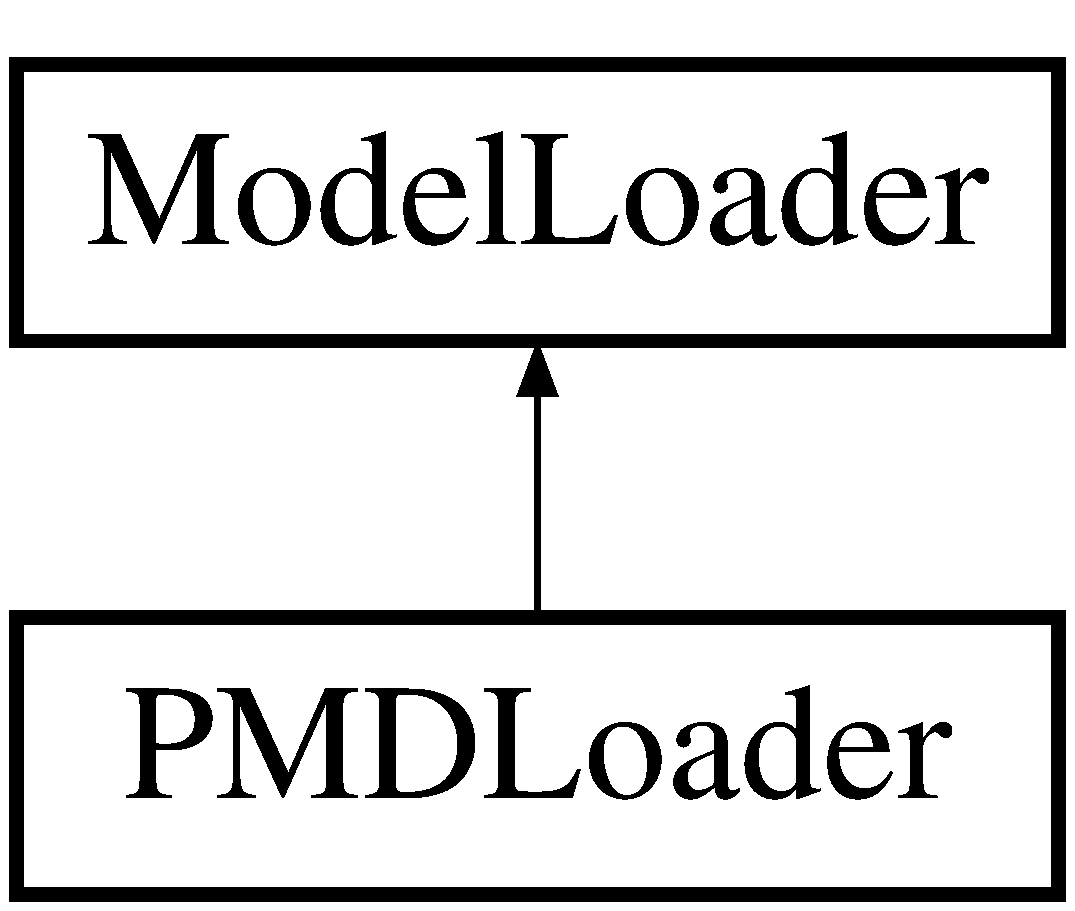
\includegraphics[height=2.000000cm]{class_p_m_d_loader}
\end{center}
\end{figure}
\subsection*{公開メンバ関数}
\begin{DoxyCompactItemize}
\item 
\mbox{\hyperlink{class_p_m_d_loader_a9a784c2a2700ee01b6c1e8139a876fa1}{$\sim$\+P\+M\+D\+Loader}} ()
\item 
std\+::shared\+\_\+ptr$<$ \mbox{\hyperlink{class_model}{Model}} $>$ \mbox{\hyperlink{class_p_m_d_loader_ae1da98c6236a58940ec521521e5c8288}{Load\+Model}} (const std\+::string \&file\+Path)
\item 
void \mbox{\hyperlink{class_p_m_d_loader_abdb6e537aef759341dfc62cd1038539c}{Clear\+Model\+Data}} ()
\end{DoxyCompactItemize}
\subsection*{静的公開メンバ関数}
\begin{DoxyCompactItemize}
\item 
static std\+::shared\+\_\+ptr$<$ \mbox{\hyperlink{class_p_m_d_loader}{P\+M\+D\+Loader}} $>$ \mbox{\hyperlink{class_p_m_d_loader_a82a5b173f9f2e05662174452cfde5578}{Create}} (std\+::shared\+\_\+ptr$<$ \mbox{\hyperlink{class_device}{Device}} $>$ device)
\end{DoxyCompactItemize}
\subsection*{その他の継承メンバ}


\subsection{構築子と解体子}
\mbox{\Hypertarget{class_p_m_d_loader_a9a784c2a2700ee01b6c1e8139a876fa1}\label{class_p_m_d_loader_a9a784c2a2700ee01b6c1e8139a876fa1}} 
\index{P\+M\+D\+Loader@{P\+M\+D\+Loader}!````~P\+M\+D\+Loader@{$\sim$\+P\+M\+D\+Loader}}
\index{````~P\+M\+D\+Loader@{$\sim$\+P\+M\+D\+Loader}!P\+M\+D\+Loader@{P\+M\+D\+Loader}}
\subsubsection{\texorpdfstring{$\sim$\+P\+M\+D\+Loader()}{~PMDLoader()}}
{\footnotesize\ttfamily P\+M\+D\+Loader\+::$\sim$\+P\+M\+D\+Loader (\begin{DoxyParamCaption}{ }\end{DoxyParamCaption})}



\subsection{関数詳解}
\mbox{\Hypertarget{class_p_m_d_loader_abdb6e537aef759341dfc62cd1038539c}\label{class_p_m_d_loader_abdb6e537aef759341dfc62cd1038539c}} 
\index{P\+M\+D\+Loader@{P\+M\+D\+Loader}!Clear\+Model\+Data@{Clear\+Model\+Data}}
\index{Clear\+Model\+Data@{Clear\+Model\+Data}!P\+M\+D\+Loader@{P\+M\+D\+Loader}}
\subsubsection{\texorpdfstring{Clear\+Model\+Data()}{ClearModelData()}}
{\footnotesize\ttfamily P\+M\+D\+Loader\+::\+Clear\+Model\+Data (\begin{DoxyParamCaption}{ }\end{DoxyParamCaption})\hspace{0.3cm}{\ttfamily [virtual]}}

読み込んだモデル情報を削除する 

\mbox{\hyperlink{class_model_loader_a6662edd78b17eeead09e822e19fc1799}{Model\+Loader}}を実装しています。

\mbox{\Hypertarget{class_p_m_d_loader_a82a5b173f9f2e05662174452cfde5578}\label{class_p_m_d_loader_a82a5b173f9f2e05662174452cfde5578}} 
\index{P\+M\+D\+Loader@{P\+M\+D\+Loader}!Create@{Create}}
\index{Create@{Create}!P\+M\+D\+Loader@{P\+M\+D\+Loader}}
\subsubsection{\texorpdfstring{Create()}{Create()}}
{\footnotesize\ttfamily std\+::shared\+\_\+ptr$<$ \mbox{\hyperlink{class_p_m_d_loader}{P\+M\+D\+Loader}} $>$ P\+M\+D\+Loader\+::\+Create (\begin{DoxyParamCaption}\item[{std\+::shared\+\_\+ptr$<$ \mbox{\hyperlink{class_device}{Device}} $>$}]{device }\end{DoxyParamCaption})\hspace{0.3cm}{\ttfamily [static]}}

\mbox{\Hypertarget{class_p_m_d_loader_ae1da98c6236a58940ec521521e5c8288}\label{class_p_m_d_loader_ae1da98c6236a58940ec521521e5c8288}} 
\index{P\+M\+D\+Loader@{P\+M\+D\+Loader}!Load\+Model@{Load\+Model}}
\index{Load\+Model@{Load\+Model}!P\+M\+D\+Loader@{P\+M\+D\+Loader}}
\subsubsection{\texorpdfstring{Load\+Model()}{LoadModel()}}
{\footnotesize\ttfamily std\+::shared\+\_\+ptr$<$ \mbox{\hyperlink{class_model}{Model}} $>$ P\+M\+D\+Loader\+::\+Load\+Model (\begin{DoxyParamCaption}\item[{const std\+::string \&}]{file\+Path }\end{DoxyParamCaption})\hspace{0.3cm}{\ttfamily [virtual]}}

モデルをロードする 
\begin{DoxyParams}[1]{引数}
\mbox{\tt in}  & {\em file\+Path} & \+: ファイルパス \\
\hline
\end{DoxyParams}
モデルデータの生成、登録 

\mbox{\hyperlink{class_model_loader_a8e2157daa8d364c36fd26922f04adcb0}{Model\+Loader}}を実装しています。



このクラス詳解は次のファイルから抽出されました\+:\begin{DoxyCompactItemize}
\item 
Source/\+Model/\mbox{\hyperlink{_p_m_d_loader_8h}{P\+M\+D\+Loader.\+h}}\item 
Source/\+Model/\mbox{\hyperlink{_p_m_d_loader_8cpp}{P\+M\+D\+Loader.\+cpp}}\end{DoxyCompactItemize}

\hypertarget{struct_p_m_d_material}{}\section{P\+M\+D\+Material 構造体}
\label{struct_p_m_d_material}\index{P\+M\+D\+Material@{P\+M\+D\+Material}}


{\ttfamily \#include $<$P\+M\+D\+Model\+Data.\+h$>$}

\subsection*{公開変数類}
\begin{DoxyCompactItemize}
\item 
\mbox{\hyperlink{struct_math_1_1_vector3}{Math\+::\+Vector3}} \mbox{\hyperlink{struct_p_m_d_material_a54704ea8dae07fba8676ca8e789725ef}{diffuse\+Color}}
\item 
float \mbox{\hyperlink{struct_p_m_d_material_afd9bbe21451115c1acd8bc9702085eb4}{alpha}}
\item 
float \mbox{\hyperlink{struct_p_m_d_material_a906fbbbac3f0e8bf814e9872a3002b79}{specularity}}
\item 
\mbox{\hyperlink{struct_math_1_1_vector3}{Math\+::\+Vector3}} \mbox{\hyperlink{struct_p_m_d_material_af6164a316f25079cd167c09ca42a6db0}{specular\+Color}}
\item 
\mbox{\hyperlink{struct_math_1_1_vector3}{Math\+::\+Vector3}} \mbox{\hyperlink{struct_p_m_d_material_ae5cdea3aceddcf4482e3dd78dea2f22a}{ambient\+Color}}
\item 
unsigned char \mbox{\hyperlink{struct_p_m_d_material_a6cd58473cb562314ae2be7340401e04c}{toon\+Index}}
\item 
unsigned char \mbox{\hyperlink{struct_p_m_d_material_a611ebccce5aa27a26891672b9699d3c9}{edge\+Flag}}
\item 
unsigned int \mbox{\hyperlink{struct_p_m_d_material_a350b72e459712e47f01e250d1b483e8b}{face\+Vertex\+Count}}
\item 
char \mbox{\hyperlink{struct_p_m_d_material_a2e15dee3872f9eb6a039d76b76b3a20e}{texture\+File\+Name}} \mbox{[}20\mbox{]}
\end{DoxyCompactItemize}


\subsection{メンバ詳解}
\mbox{\Hypertarget{struct_p_m_d_material_afd9bbe21451115c1acd8bc9702085eb4}\label{struct_p_m_d_material_afd9bbe21451115c1acd8bc9702085eb4}} 
\index{P\+M\+D\+Material@{P\+M\+D\+Material}!alpha@{alpha}}
\index{alpha@{alpha}!P\+M\+D\+Material@{P\+M\+D\+Material}}
\subsubsection{\texorpdfstring{alpha}{alpha}}
{\footnotesize\ttfamily float P\+M\+D\+Material\+::alpha}

\mbox{\Hypertarget{struct_p_m_d_material_ae5cdea3aceddcf4482e3dd78dea2f22a}\label{struct_p_m_d_material_ae5cdea3aceddcf4482e3dd78dea2f22a}} 
\index{P\+M\+D\+Material@{P\+M\+D\+Material}!ambient\+Color@{ambient\+Color}}
\index{ambient\+Color@{ambient\+Color}!P\+M\+D\+Material@{P\+M\+D\+Material}}
\subsubsection{\texorpdfstring{ambient\+Color}{ambientColor}}
{\footnotesize\ttfamily \mbox{\hyperlink{struct_math_1_1_vector3}{Math\+::\+Vector3}} P\+M\+D\+Material\+::ambient\+Color}

\mbox{\Hypertarget{struct_p_m_d_material_a54704ea8dae07fba8676ca8e789725ef}\label{struct_p_m_d_material_a54704ea8dae07fba8676ca8e789725ef}} 
\index{P\+M\+D\+Material@{P\+M\+D\+Material}!diffuse\+Color@{diffuse\+Color}}
\index{diffuse\+Color@{diffuse\+Color}!P\+M\+D\+Material@{P\+M\+D\+Material}}
\subsubsection{\texorpdfstring{diffuse\+Color}{diffuseColor}}
{\footnotesize\ttfamily \mbox{\hyperlink{struct_math_1_1_vector3}{Math\+::\+Vector3}} P\+M\+D\+Material\+::diffuse\+Color}

\mbox{\Hypertarget{struct_p_m_d_material_a611ebccce5aa27a26891672b9699d3c9}\label{struct_p_m_d_material_a611ebccce5aa27a26891672b9699d3c9}} 
\index{P\+M\+D\+Material@{P\+M\+D\+Material}!edge\+Flag@{edge\+Flag}}
\index{edge\+Flag@{edge\+Flag}!P\+M\+D\+Material@{P\+M\+D\+Material}}
\subsubsection{\texorpdfstring{edge\+Flag}{edgeFlag}}
{\footnotesize\ttfamily unsigned char P\+M\+D\+Material\+::edge\+Flag}

\mbox{\Hypertarget{struct_p_m_d_material_a350b72e459712e47f01e250d1b483e8b}\label{struct_p_m_d_material_a350b72e459712e47f01e250d1b483e8b}} 
\index{P\+M\+D\+Material@{P\+M\+D\+Material}!face\+Vertex\+Count@{face\+Vertex\+Count}}
\index{face\+Vertex\+Count@{face\+Vertex\+Count}!P\+M\+D\+Material@{P\+M\+D\+Material}}
\subsubsection{\texorpdfstring{face\+Vertex\+Count}{faceVertexCount}}
{\footnotesize\ttfamily unsigned int P\+M\+D\+Material\+::face\+Vertex\+Count}

\mbox{\Hypertarget{struct_p_m_d_material_af6164a316f25079cd167c09ca42a6db0}\label{struct_p_m_d_material_af6164a316f25079cd167c09ca42a6db0}} 
\index{P\+M\+D\+Material@{P\+M\+D\+Material}!specular\+Color@{specular\+Color}}
\index{specular\+Color@{specular\+Color}!P\+M\+D\+Material@{P\+M\+D\+Material}}
\subsubsection{\texorpdfstring{specular\+Color}{specularColor}}
{\footnotesize\ttfamily \mbox{\hyperlink{struct_math_1_1_vector3}{Math\+::\+Vector3}} P\+M\+D\+Material\+::specular\+Color}

\mbox{\Hypertarget{struct_p_m_d_material_a906fbbbac3f0e8bf814e9872a3002b79}\label{struct_p_m_d_material_a906fbbbac3f0e8bf814e9872a3002b79}} 
\index{P\+M\+D\+Material@{P\+M\+D\+Material}!specularity@{specularity}}
\index{specularity@{specularity}!P\+M\+D\+Material@{P\+M\+D\+Material}}
\subsubsection{\texorpdfstring{specularity}{specularity}}
{\footnotesize\ttfamily float P\+M\+D\+Material\+::specularity}

\mbox{\Hypertarget{struct_p_m_d_material_a2e15dee3872f9eb6a039d76b76b3a20e}\label{struct_p_m_d_material_a2e15dee3872f9eb6a039d76b76b3a20e}} 
\index{P\+M\+D\+Material@{P\+M\+D\+Material}!texture\+File\+Name@{texture\+File\+Name}}
\index{texture\+File\+Name@{texture\+File\+Name}!P\+M\+D\+Material@{P\+M\+D\+Material}}
\subsubsection{\texorpdfstring{texture\+File\+Name}{textureFileName}}
{\footnotesize\ttfamily char P\+M\+D\+Material\+::texture\+File\+Name\mbox{[}20\mbox{]}}

\mbox{\Hypertarget{struct_p_m_d_material_a6cd58473cb562314ae2be7340401e04c}\label{struct_p_m_d_material_a6cd58473cb562314ae2be7340401e04c}} 
\index{P\+M\+D\+Material@{P\+M\+D\+Material}!toon\+Index@{toon\+Index}}
\index{toon\+Index@{toon\+Index}!P\+M\+D\+Material@{P\+M\+D\+Material}}
\subsubsection{\texorpdfstring{toon\+Index}{toonIndex}}
{\footnotesize\ttfamily unsigned char P\+M\+D\+Material\+::toon\+Index}



この構造体詳解は次のファイルから抽出されました\+:\begin{DoxyCompactItemize}
\item 
Source/\+Model/\mbox{\hyperlink{_p_m_d_model_data_8h}{P\+M\+D\+Model\+Data.\+h}}\end{DoxyCompactItemize}

\hypertarget{class_p_m_d_model_data}{}\section{P\+M\+D\+Model\+Data クラス}
\label{class_p_m_d_model_data}\index{P\+M\+D\+Model\+Data@{P\+M\+D\+Model\+Data}}


{\ttfamily \#include $<$P\+M\+D\+Model\+Data.\+h$>$}

P\+M\+D\+Model\+Data の継承関係図\begin{figure}[H]
\begin{center}
\leavevmode
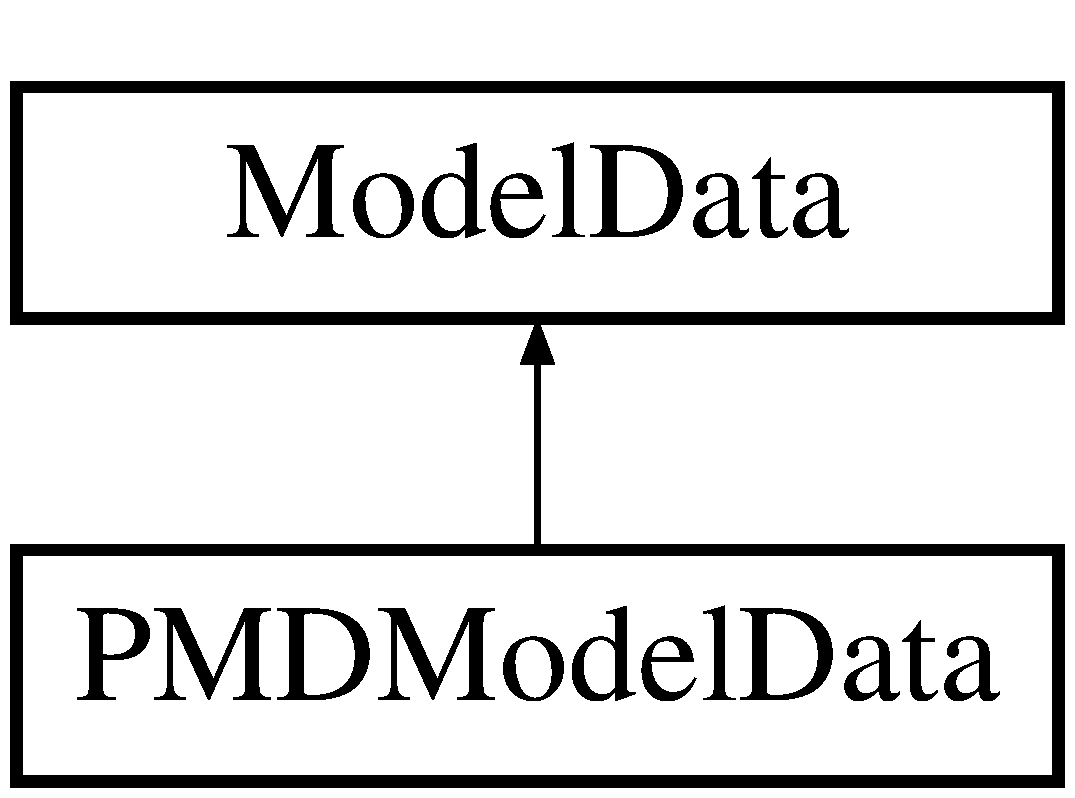
\includegraphics[height=2.000000cm]{class_p_m_d_model_data}
\end{center}
\end{figure}
\subsection*{公開メンバ関数}
\begin{DoxyCompactItemize}
\item 
\mbox{\hyperlink{class_p_m_d_model_data_a75af9f2a3f48724d2c4670cc4c117a0f}{P\+M\+D\+Model\+Data}} (std\+::shared\+\_\+ptr$<$ \mbox{\hyperlink{class_device}{Device}} $>$ device, const \mbox{\hyperlink{struct_p_m_d_model_info}{P\+M\+D\+Model\+Info}} \&model\+Info)
\item 
\mbox{\hyperlink{class_p_m_d_model_data_a5cc7bb8b8046d533f3d38f5e056cf627}{$\sim$\+P\+M\+D\+Model\+Data}} ()
\item 
void \mbox{\hyperlink{class_p_m_d_model_data_a7c3e55a09f65738c2117bdd7bb71b058}{Set\+Vertex\+Data}} (const std\+::vector$<$ \mbox{\hyperlink{struct_p_m_d_vertex}{P\+M\+D\+Vertex}} $>$ \&vertex\+Data)
\item 
void \mbox{\hyperlink{class_p_m_d_model_data_a120b4a461669a4bb68210602b17425f1}{Set\+Index\+Data}} (const std\+::vector$<$ unsigned short $>$ \&index\+Data)
\item 
void \mbox{\hyperlink{class_p_m_d_model_data_a83a950e111380bb2a28ecab045e5c3b4}{Set\+Material\+Data}} (std\+::shared\+\_\+ptr$<$ \mbox{\hyperlink{class_device}{Device}} $>$ device, const std\+::vector$<$ \mbox{\hyperlink{struct_p_m_d_material}{P\+M\+D\+Material}} $>$ \&materials, const std\+::string \&model\+Path)
\item 
void \mbox{\hyperlink{class_p_m_d_model_data_ae811d49854ae659f20ac9be60a5fb146}{Draw}} (Com\+Ptr$<$ I\+D3\+D12\+Graphics\+Command\+List $>$ command\+List, const \mbox{\hyperlink{struct_instance_data}{Instance\+Data}} \&instance\+Data) const
\begin{DoxyCompactList}\small\item\em 描画処理 \end{DoxyCompactList}\end{DoxyCompactItemize}
\subsection*{静的公開メンバ関数}
\begin{DoxyCompactItemize}
\item 
static std\+::shared\+\_\+ptr$<$ \mbox{\hyperlink{class_p_m_d_model_data}{P\+M\+D\+Model\+Data}} $>$ \mbox{\hyperlink{class_p_m_d_model_data_a026bc021f9c229a820054b50821d9171}{Create}} (std\+::shared\+\_\+ptr$<$ \mbox{\hyperlink{class_device}{Device}} $>$ device, const \mbox{\hyperlink{struct_p_m_d_model_info}{P\+M\+D\+Model\+Info}} \&model\+Info)
\end{DoxyCompactItemize}
\subsection*{その他の継承メンバ}


\subsection{構築子と解体子}
\mbox{\Hypertarget{class_p_m_d_model_data_a75af9f2a3f48724d2c4670cc4c117a0f}\label{class_p_m_d_model_data_a75af9f2a3f48724d2c4670cc4c117a0f}} 
\index{P\+M\+D\+Model\+Data@{P\+M\+D\+Model\+Data}!P\+M\+D\+Model\+Data@{P\+M\+D\+Model\+Data}}
\index{P\+M\+D\+Model\+Data@{P\+M\+D\+Model\+Data}!P\+M\+D\+Model\+Data@{P\+M\+D\+Model\+Data}}
\subsubsection{\texorpdfstring{P\+M\+D\+Model\+Data()}{PMDModelData()}}
{\footnotesize\ttfamily P\+M\+D\+Model\+Data\+::\+P\+M\+D\+Model\+Data (\begin{DoxyParamCaption}\item[{std\+::shared\+\_\+ptr$<$ \mbox{\hyperlink{class_device}{Device}} $>$}]{device,  }\item[{const \mbox{\hyperlink{struct_p_m_d_model_info}{P\+M\+D\+Model\+Info}} \&}]{model\+Info }\end{DoxyParamCaption})}

\mbox{\Hypertarget{class_p_m_d_model_data_a5cc7bb8b8046d533f3d38f5e056cf627}\label{class_p_m_d_model_data_a5cc7bb8b8046d533f3d38f5e056cf627}} 
\index{P\+M\+D\+Model\+Data@{P\+M\+D\+Model\+Data}!````~P\+M\+D\+Model\+Data@{$\sim$\+P\+M\+D\+Model\+Data}}
\index{````~P\+M\+D\+Model\+Data@{$\sim$\+P\+M\+D\+Model\+Data}!P\+M\+D\+Model\+Data@{P\+M\+D\+Model\+Data}}
\subsubsection{\texorpdfstring{$\sim$\+P\+M\+D\+Model\+Data()}{~PMDModelData()}}
{\footnotesize\ttfamily P\+M\+D\+Model\+Data\+::$\sim$\+P\+M\+D\+Model\+Data (\begin{DoxyParamCaption}{ }\end{DoxyParamCaption})}



\subsection{関数詳解}
\mbox{\Hypertarget{class_p_m_d_model_data_a026bc021f9c229a820054b50821d9171}\label{class_p_m_d_model_data_a026bc021f9c229a820054b50821d9171}} 
\index{P\+M\+D\+Model\+Data@{P\+M\+D\+Model\+Data}!Create@{Create}}
\index{Create@{Create}!P\+M\+D\+Model\+Data@{P\+M\+D\+Model\+Data}}
\subsubsection{\texorpdfstring{Create()}{Create()}}
{\footnotesize\ttfamily std\+::shared\+\_\+ptr$<$ \mbox{\hyperlink{class_p_m_d_model_data}{P\+M\+D\+Model\+Data}} $>$ P\+M\+D\+Model\+Data\+::\+Create (\begin{DoxyParamCaption}\item[{std\+::shared\+\_\+ptr$<$ \mbox{\hyperlink{class_device}{Device}} $>$}]{device,  }\item[{const \mbox{\hyperlink{struct_p_m_d_model_info}{P\+M\+D\+Model\+Info}} \&}]{model\+Info }\end{DoxyParamCaption})\hspace{0.3cm}{\ttfamily [static]}}

\mbox{\Hypertarget{class_p_m_d_model_data_ae811d49854ae659f20ac9be60a5fb146}\label{class_p_m_d_model_data_ae811d49854ae659f20ac9be60a5fb146}} 
\index{P\+M\+D\+Model\+Data@{P\+M\+D\+Model\+Data}!Draw@{Draw}}
\index{Draw@{Draw}!P\+M\+D\+Model\+Data@{P\+M\+D\+Model\+Data}}
\subsubsection{\texorpdfstring{Draw()}{Draw()}}
{\footnotesize\ttfamily void P\+M\+D\+Model\+Data\+::\+Draw (\begin{DoxyParamCaption}\item[{Com\+Ptr$<$ I\+D3\+D12\+Graphics\+Command\+List $>$}]{graphics\+Command\+List,  }\item[{const \mbox{\hyperlink{struct_instance_data}{Instance\+Data}} \&}]{instance\+Data }\end{DoxyParamCaption}) const\hspace{0.3cm}{\ttfamily [virtual]}}



描画処理 



\mbox{\hyperlink{class_model_data_a774032c8dac7355ad2657c83cf0d1e21}{Model\+Data}}を再実装しています。

\mbox{\Hypertarget{class_p_m_d_model_data_a120b4a461669a4bb68210602b17425f1}\label{class_p_m_d_model_data_a120b4a461669a4bb68210602b17425f1}} 
\index{P\+M\+D\+Model\+Data@{P\+M\+D\+Model\+Data}!Set\+Index\+Data@{Set\+Index\+Data}}
\index{Set\+Index\+Data@{Set\+Index\+Data}!P\+M\+D\+Model\+Data@{P\+M\+D\+Model\+Data}}
\subsubsection{\texorpdfstring{Set\+Index\+Data()}{SetIndexData()}}
{\footnotesize\ttfamily void P\+M\+D\+Model\+Data\+::\+Set\+Index\+Data (\begin{DoxyParamCaption}\item[{const std\+::vector$<$ unsigned short $>$ \&}]{index\+Data }\end{DoxyParamCaption})}

\mbox{\Hypertarget{class_p_m_d_model_data_a83a950e111380bb2a28ecab045e5c3b4}\label{class_p_m_d_model_data_a83a950e111380bb2a28ecab045e5c3b4}} 
\index{P\+M\+D\+Model\+Data@{P\+M\+D\+Model\+Data}!Set\+Material\+Data@{Set\+Material\+Data}}
\index{Set\+Material\+Data@{Set\+Material\+Data}!P\+M\+D\+Model\+Data@{P\+M\+D\+Model\+Data}}
\subsubsection{\texorpdfstring{Set\+Material\+Data()}{SetMaterialData()}}
{\footnotesize\ttfamily void P\+M\+D\+Model\+Data\+::\+Set\+Material\+Data (\begin{DoxyParamCaption}\item[{std\+::shared\+\_\+ptr$<$ \mbox{\hyperlink{class_device}{Device}} $>$}]{device,  }\item[{const std\+::vector$<$ \mbox{\hyperlink{struct_p_m_d_material}{P\+M\+D\+Material}} $>$ \&}]{materials,  }\item[{const std\+::string \&}]{model\+Path }\end{DoxyParamCaption})}

\mbox{\Hypertarget{class_p_m_d_model_data_a7c3e55a09f65738c2117bdd7bb71b058}\label{class_p_m_d_model_data_a7c3e55a09f65738c2117bdd7bb71b058}} 
\index{P\+M\+D\+Model\+Data@{P\+M\+D\+Model\+Data}!Set\+Vertex\+Data@{Set\+Vertex\+Data}}
\index{Set\+Vertex\+Data@{Set\+Vertex\+Data}!P\+M\+D\+Model\+Data@{P\+M\+D\+Model\+Data}}
\subsubsection{\texorpdfstring{Set\+Vertex\+Data()}{SetVertexData()}}
{\footnotesize\ttfamily void P\+M\+D\+Model\+Data\+::\+Set\+Vertex\+Data (\begin{DoxyParamCaption}\item[{const std\+::vector$<$ \mbox{\hyperlink{struct_p_m_d_vertex}{P\+M\+D\+Vertex}} $>$ \&}]{vertex\+Data }\end{DoxyParamCaption})}



このクラス詳解は次のファイルから抽出されました\+:\begin{DoxyCompactItemize}
\item 
Source/\+Model/\mbox{\hyperlink{_p_m_d_model_data_8h}{P\+M\+D\+Model\+Data.\+h}}\item 
Source/\+Model/\mbox{\hyperlink{_p_m_d_model_data_8cpp}{P\+M\+D\+Model\+Data.\+cpp}}\end{DoxyCompactItemize}

\hypertarget{struct_p_m_d_model_info}{}\section{P\+M\+D\+Model\+Info 構造体}
\label{struct_p_m_d_model_info}\index{P\+M\+D\+Model\+Info@{P\+M\+D\+Model\+Info}}


{\ttfamily \#include $<$P\+M\+D\+Model\+Data.\+h$>$}

\subsection*{公開変数類}
\begin{DoxyCompactItemize}
\item 
std\+::string \mbox{\hyperlink{struct_p_m_d_model_info_a756ac77e858d04d751c7bf4bc01f22d7}{model\+Path}}
\item 
std\+::vector$<$ \mbox{\hyperlink{struct_p_m_d_vertex}{P\+M\+D\+Vertex}} $>$ \mbox{\hyperlink{struct_p_m_d_model_info_a2862ab3d4b00b5600723eed89b4888ab}{vertex\+Data}}
\item 
std\+::vector$<$ unsigned short $>$ \mbox{\hyperlink{struct_p_m_d_model_info_a84f1297444562cd6012f13b45d988759}{index\+Data}}
\item 
std\+::vector$<$ \mbox{\hyperlink{struct_p_m_d_material}{P\+M\+D\+Material}} $>$ \mbox{\hyperlink{struct_p_m_d_model_info_ae9e41e468da41dd38df7f39243050def}{materials}}
\end{DoxyCompactItemize}


\subsection{メンバ詳解}
\mbox{\Hypertarget{struct_p_m_d_model_info_a84f1297444562cd6012f13b45d988759}\label{struct_p_m_d_model_info_a84f1297444562cd6012f13b45d988759}} 
\index{P\+M\+D\+Model\+Info@{P\+M\+D\+Model\+Info}!index\+Data@{index\+Data}}
\index{index\+Data@{index\+Data}!P\+M\+D\+Model\+Info@{P\+M\+D\+Model\+Info}}
\subsubsection{\texorpdfstring{index\+Data}{indexData}}
{\footnotesize\ttfamily std\+::vector$<$unsigned short$>$ P\+M\+D\+Model\+Info\+::index\+Data}

\mbox{\Hypertarget{struct_p_m_d_model_info_ae9e41e468da41dd38df7f39243050def}\label{struct_p_m_d_model_info_ae9e41e468da41dd38df7f39243050def}} 
\index{P\+M\+D\+Model\+Info@{P\+M\+D\+Model\+Info}!materials@{materials}}
\index{materials@{materials}!P\+M\+D\+Model\+Info@{P\+M\+D\+Model\+Info}}
\subsubsection{\texorpdfstring{materials}{materials}}
{\footnotesize\ttfamily std\+::vector$<$\mbox{\hyperlink{struct_p_m_d_material}{P\+M\+D\+Material}}$>$ P\+M\+D\+Model\+Info\+::materials}

\mbox{\Hypertarget{struct_p_m_d_model_info_a756ac77e858d04d751c7bf4bc01f22d7}\label{struct_p_m_d_model_info_a756ac77e858d04d751c7bf4bc01f22d7}} 
\index{P\+M\+D\+Model\+Info@{P\+M\+D\+Model\+Info}!model\+Path@{model\+Path}}
\index{model\+Path@{model\+Path}!P\+M\+D\+Model\+Info@{P\+M\+D\+Model\+Info}}
\subsubsection{\texorpdfstring{model\+Path}{modelPath}}
{\footnotesize\ttfamily std\+::string P\+M\+D\+Model\+Info\+::model\+Path}

\mbox{\Hypertarget{struct_p_m_d_model_info_a2862ab3d4b00b5600723eed89b4888ab}\label{struct_p_m_d_model_info_a2862ab3d4b00b5600723eed89b4888ab}} 
\index{P\+M\+D\+Model\+Info@{P\+M\+D\+Model\+Info}!vertex\+Data@{vertex\+Data}}
\index{vertex\+Data@{vertex\+Data}!P\+M\+D\+Model\+Info@{P\+M\+D\+Model\+Info}}
\subsubsection{\texorpdfstring{vertex\+Data}{vertexData}}
{\footnotesize\ttfamily std\+::vector$<$\mbox{\hyperlink{struct_p_m_d_vertex}{P\+M\+D\+Vertex}}$>$ P\+M\+D\+Model\+Info\+::vertex\+Data}



この構造体詳解は次のファイルから抽出されました\+:\begin{DoxyCompactItemize}
\item 
Source/\+Model/\mbox{\hyperlink{_p_m_d_model_data_8h}{P\+M\+D\+Model\+Data.\+h}}\end{DoxyCompactItemize}

\hypertarget{struct_p_m_d_shader_material_data}{}\section{P\+M\+D\+Shader\+Material\+Data 構造体}
\label{struct_p_m_d_shader_material_data}\index{P\+M\+D\+Shader\+Material\+Data@{P\+M\+D\+Shader\+Material\+Data}}


{\ttfamily \#include $<$P\+M\+D\+Model\+Data.\+h$>$}

\subsection*{公開変数類}
\begin{DoxyCompactItemize}
\item 
\mbox{\hyperlink{struct_math_1_1_vector3}{Math\+::\+Vector3}} \mbox{\hyperlink{struct_p_m_d_shader_material_data_aed48b81c7419be094332641735c851c3}{diffuse\+Color}}
\item 
float \mbox{\hyperlink{struct_p_m_d_shader_material_data_a7cecd80aa0d657d983070859f5b2f298}{alpha}}
\item 
float \mbox{\hyperlink{struct_p_m_d_shader_material_data_a8a1f669aaaebb002f9bc8787cc9774d4}{specularity}}
\item 
\mbox{\hyperlink{struct_math_1_1_vector3}{Math\+::\+Vector3}} \mbox{\hyperlink{struct_p_m_d_shader_material_data_a455c3ff915b9c29a608cefa02b641420}{specular\+Color}}
\item 
\mbox{\hyperlink{struct_math_1_1_vector3}{Math\+::\+Vector3}} \mbox{\hyperlink{struct_p_m_d_shader_material_data_adb05d453d38b015e0ec08e7e5565dcce}{ambient\+Color}}
\item 
int \mbox{\hyperlink{struct_p_m_d_shader_material_data_a5ee42a778ab59caea2465f5fd8edac72}{is\+Use\+Texture}}
\item 
int \mbox{\hyperlink{struct_p_m_d_shader_material_data_ad0e85b0bc186b60ca467f37d6fda43d0}{sphere\+Flag}}
\end{DoxyCompactItemize}


\subsection{メンバ詳解}
\mbox{\Hypertarget{struct_p_m_d_shader_material_data_a7cecd80aa0d657d983070859f5b2f298}\label{struct_p_m_d_shader_material_data_a7cecd80aa0d657d983070859f5b2f298}} 
\index{P\+M\+D\+Shader\+Material\+Data@{P\+M\+D\+Shader\+Material\+Data}!alpha@{alpha}}
\index{alpha@{alpha}!P\+M\+D\+Shader\+Material\+Data@{P\+M\+D\+Shader\+Material\+Data}}
\subsubsection{\texorpdfstring{alpha}{alpha}}
{\footnotesize\ttfamily float P\+M\+D\+Shader\+Material\+Data\+::alpha}

\mbox{\Hypertarget{struct_p_m_d_shader_material_data_adb05d453d38b015e0ec08e7e5565dcce}\label{struct_p_m_d_shader_material_data_adb05d453d38b015e0ec08e7e5565dcce}} 
\index{P\+M\+D\+Shader\+Material\+Data@{P\+M\+D\+Shader\+Material\+Data}!ambient\+Color@{ambient\+Color}}
\index{ambient\+Color@{ambient\+Color}!P\+M\+D\+Shader\+Material\+Data@{P\+M\+D\+Shader\+Material\+Data}}
\subsubsection{\texorpdfstring{ambient\+Color}{ambientColor}}
{\footnotesize\ttfamily \mbox{\hyperlink{struct_math_1_1_vector3}{Math\+::\+Vector3}} P\+M\+D\+Shader\+Material\+Data\+::ambient\+Color}

\mbox{\Hypertarget{struct_p_m_d_shader_material_data_aed48b81c7419be094332641735c851c3}\label{struct_p_m_d_shader_material_data_aed48b81c7419be094332641735c851c3}} 
\index{P\+M\+D\+Shader\+Material\+Data@{P\+M\+D\+Shader\+Material\+Data}!diffuse\+Color@{diffuse\+Color}}
\index{diffuse\+Color@{diffuse\+Color}!P\+M\+D\+Shader\+Material\+Data@{P\+M\+D\+Shader\+Material\+Data}}
\subsubsection{\texorpdfstring{diffuse\+Color}{diffuseColor}}
{\footnotesize\ttfamily \mbox{\hyperlink{struct_math_1_1_vector3}{Math\+::\+Vector3}} P\+M\+D\+Shader\+Material\+Data\+::diffuse\+Color}

\mbox{\Hypertarget{struct_p_m_d_shader_material_data_a5ee42a778ab59caea2465f5fd8edac72}\label{struct_p_m_d_shader_material_data_a5ee42a778ab59caea2465f5fd8edac72}} 
\index{P\+M\+D\+Shader\+Material\+Data@{P\+M\+D\+Shader\+Material\+Data}!is\+Use\+Texture@{is\+Use\+Texture}}
\index{is\+Use\+Texture@{is\+Use\+Texture}!P\+M\+D\+Shader\+Material\+Data@{P\+M\+D\+Shader\+Material\+Data}}
\subsubsection{\texorpdfstring{is\+Use\+Texture}{isUseTexture}}
{\footnotesize\ttfamily int P\+M\+D\+Shader\+Material\+Data\+::is\+Use\+Texture}

\mbox{\Hypertarget{struct_p_m_d_shader_material_data_a455c3ff915b9c29a608cefa02b641420}\label{struct_p_m_d_shader_material_data_a455c3ff915b9c29a608cefa02b641420}} 
\index{P\+M\+D\+Shader\+Material\+Data@{P\+M\+D\+Shader\+Material\+Data}!specular\+Color@{specular\+Color}}
\index{specular\+Color@{specular\+Color}!P\+M\+D\+Shader\+Material\+Data@{P\+M\+D\+Shader\+Material\+Data}}
\subsubsection{\texorpdfstring{specular\+Color}{specularColor}}
{\footnotesize\ttfamily \mbox{\hyperlink{struct_math_1_1_vector3}{Math\+::\+Vector3}} P\+M\+D\+Shader\+Material\+Data\+::specular\+Color}

\mbox{\Hypertarget{struct_p_m_d_shader_material_data_a8a1f669aaaebb002f9bc8787cc9774d4}\label{struct_p_m_d_shader_material_data_a8a1f669aaaebb002f9bc8787cc9774d4}} 
\index{P\+M\+D\+Shader\+Material\+Data@{P\+M\+D\+Shader\+Material\+Data}!specularity@{specularity}}
\index{specularity@{specularity}!P\+M\+D\+Shader\+Material\+Data@{P\+M\+D\+Shader\+Material\+Data}}
\subsubsection{\texorpdfstring{specularity}{specularity}}
{\footnotesize\ttfamily float P\+M\+D\+Shader\+Material\+Data\+::specularity}

\mbox{\Hypertarget{struct_p_m_d_shader_material_data_ad0e85b0bc186b60ca467f37d6fda43d0}\label{struct_p_m_d_shader_material_data_ad0e85b0bc186b60ca467f37d6fda43d0}} 
\index{P\+M\+D\+Shader\+Material\+Data@{P\+M\+D\+Shader\+Material\+Data}!sphere\+Flag@{sphere\+Flag}}
\index{sphere\+Flag@{sphere\+Flag}!P\+M\+D\+Shader\+Material\+Data@{P\+M\+D\+Shader\+Material\+Data}}
\subsubsection{\texorpdfstring{sphere\+Flag}{sphereFlag}}
{\footnotesize\ttfamily int P\+M\+D\+Shader\+Material\+Data\+::sphere\+Flag}



この構造体詳解は次のファイルから抽出されました\+:\begin{DoxyCompactItemize}
\item 
Source/\+Model/\mbox{\hyperlink{_p_m_d_model_data_8h}{P\+M\+D\+Model\+Data.\+h}}\end{DoxyCompactItemize}

\hypertarget{struct_p_m_d_vertex}{}\section{P\+M\+D\+Vertex 構造体}
\label{struct_p_m_d_vertex}\index{P\+M\+D\+Vertex@{P\+M\+D\+Vertex}}


{\ttfamily \#include $<$P\+M\+D\+Model\+Data.\+h$>$}

\subsection*{公開変数類}
\begin{DoxyCompactItemize}
\item 
\mbox{\hyperlink{struct_math_1_1_vector3}{Math\+::\+Vector3}} \mbox{\hyperlink{struct_p_m_d_vertex_af9eb3741205512ac55530a52d0102bc0}{position}}
\item 
\mbox{\hyperlink{struct_math_1_1_vector3}{Math\+::\+Vector3}} \mbox{\hyperlink{struct_p_m_d_vertex_afa1e149594fbe11bc4cb3747d8e85c56}{normal}}
\item 
\mbox{\hyperlink{struct_math_1_1_vector2}{Math\+::\+Vector2}} \mbox{\hyperlink{struct_p_m_d_vertex_a42049ecad8df8c3708079463a7b85281}{uv}}
\item 
unsigned short \mbox{\hyperlink{struct_p_m_d_vertex_a9b3e6edca54f4f29192b47388b5e757c}{bone\+Index}} \mbox{[}2\mbox{]}
\item 
unsigned char \mbox{\hyperlink{struct_p_m_d_vertex_af60fe66bc32b1cd4b4f7025e68b887a4}{bone\+Weight}}
\item 
unsigned char \mbox{\hyperlink{struct_p_m_d_vertex_a08c82b0d461f3dab3565918ef5a6cec0}{edge\+Flag}}
\end{DoxyCompactItemize}


\subsection{詳解}
P\+M\+D頂点情報 

\subsection{メンバ詳解}
\mbox{\Hypertarget{struct_p_m_d_vertex_a9b3e6edca54f4f29192b47388b5e757c}\label{struct_p_m_d_vertex_a9b3e6edca54f4f29192b47388b5e757c}} 
\index{P\+M\+D\+Vertex@{P\+M\+D\+Vertex}!bone\+Index@{bone\+Index}}
\index{bone\+Index@{bone\+Index}!P\+M\+D\+Vertex@{P\+M\+D\+Vertex}}
\subsubsection{\texorpdfstring{bone\+Index}{boneIndex}}
{\footnotesize\ttfamily unsigned short P\+M\+D\+Vertex\+::bone\+Index\mbox{[}2\mbox{]}}

\mbox{\Hypertarget{struct_p_m_d_vertex_af60fe66bc32b1cd4b4f7025e68b887a4}\label{struct_p_m_d_vertex_af60fe66bc32b1cd4b4f7025e68b887a4}} 
\index{P\+M\+D\+Vertex@{P\+M\+D\+Vertex}!bone\+Weight@{bone\+Weight}}
\index{bone\+Weight@{bone\+Weight}!P\+M\+D\+Vertex@{P\+M\+D\+Vertex}}
\subsubsection{\texorpdfstring{bone\+Weight}{boneWeight}}
{\footnotesize\ttfamily unsigned char P\+M\+D\+Vertex\+::bone\+Weight}

\mbox{\Hypertarget{struct_p_m_d_vertex_a08c82b0d461f3dab3565918ef5a6cec0}\label{struct_p_m_d_vertex_a08c82b0d461f3dab3565918ef5a6cec0}} 
\index{P\+M\+D\+Vertex@{P\+M\+D\+Vertex}!edge\+Flag@{edge\+Flag}}
\index{edge\+Flag@{edge\+Flag}!P\+M\+D\+Vertex@{P\+M\+D\+Vertex}}
\subsubsection{\texorpdfstring{edge\+Flag}{edgeFlag}}
{\footnotesize\ttfamily unsigned char P\+M\+D\+Vertex\+::edge\+Flag}

\mbox{\Hypertarget{struct_p_m_d_vertex_afa1e149594fbe11bc4cb3747d8e85c56}\label{struct_p_m_d_vertex_afa1e149594fbe11bc4cb3747d8e85c56}} 
\index{P\+M\+D\+Vertex@{P\+M\+D\+Vertex}!normal@{normal}}
\index{normal@{normal}!P\+M\+D\+Vertex@{P\+M\+D\+Vertex}}
\subsubsection{\texorpdfstring{normal}{normal}}
{\footnotesize\ttfamily \mbox{\hyperlink{struct_math_1_1_vector3}{Math\+::\+Vector3}} P\+M\+D\+Vertex\+::normal}

\mbox{\Hypertarget{struct_p_m_d_vertex_af9eb3741205512ac55530a52d0102bc0}\label{struct_p_m_d_vertex_af9eb3741205512ac55530a52d0102bc0}} 
\index{P\+M\+D\+Vertex@{P\+M\+D\+Vertex}!position@{position}}
\index{position@{position}!P\+M\+D\+Vertex@{P\+M\+D\+Vertex}}
\subsubsection{\texorpdfstring{position}{position}}
{\footnotesize\ttfamily \mbox{\hyperlink{struct_math_1_1_vector3}{Math\+::\+Vector3}} P\+M\+D\+Vertex\+::position}

\mbox{\Hypertarget{struct_p_m_d_vertex_a42049ecad8df8c3708079463a7b85281}\label{struct_p_m_d_vertex_a42049ecad8df8c3708079463a7b85281}} 
\index{P\+M\+D\+Vertex@{P\+M\+D\+Vertex}!uv@{uv}}
\index{uv@{uv}!P\+M\+D\+Vertex@{P\+M\+D\+Vertex}}
\subsubsection{\texorpdfstring{uv}{uv}}
{\footnotesize\ttfamily \mbox{\hyperlink{struct_math_1_1_vector2}{Math\+::\+Vector2}} P\+M\+D\+Vertex\+::uv}



この構造体詳解は次のファイルから抽出されました\+:\begin{DoxyCompactItemize}
\item 
Source/\+Model/\mbox{\hyperlink{_p_m_d_model_data_8h}{P\+M\+D\+Model\+Data.\+h}}\end{DoxyCompactItemize}

\hypertarget{class_p_m_x_loader}{}\section{P\+M\+X\+Loader クラス}
\label{class_p_m_x_loader}\index{P\+M\+X\+Loader@{P\+M\+X\+Loader}}


{\ttfamily \#include $<$P\+M\+X\+Loader.\+h$>$}

P\+M\+X\+Loader の継承関係図\begin{figure}[H]
\begin{center}
\leavevmode
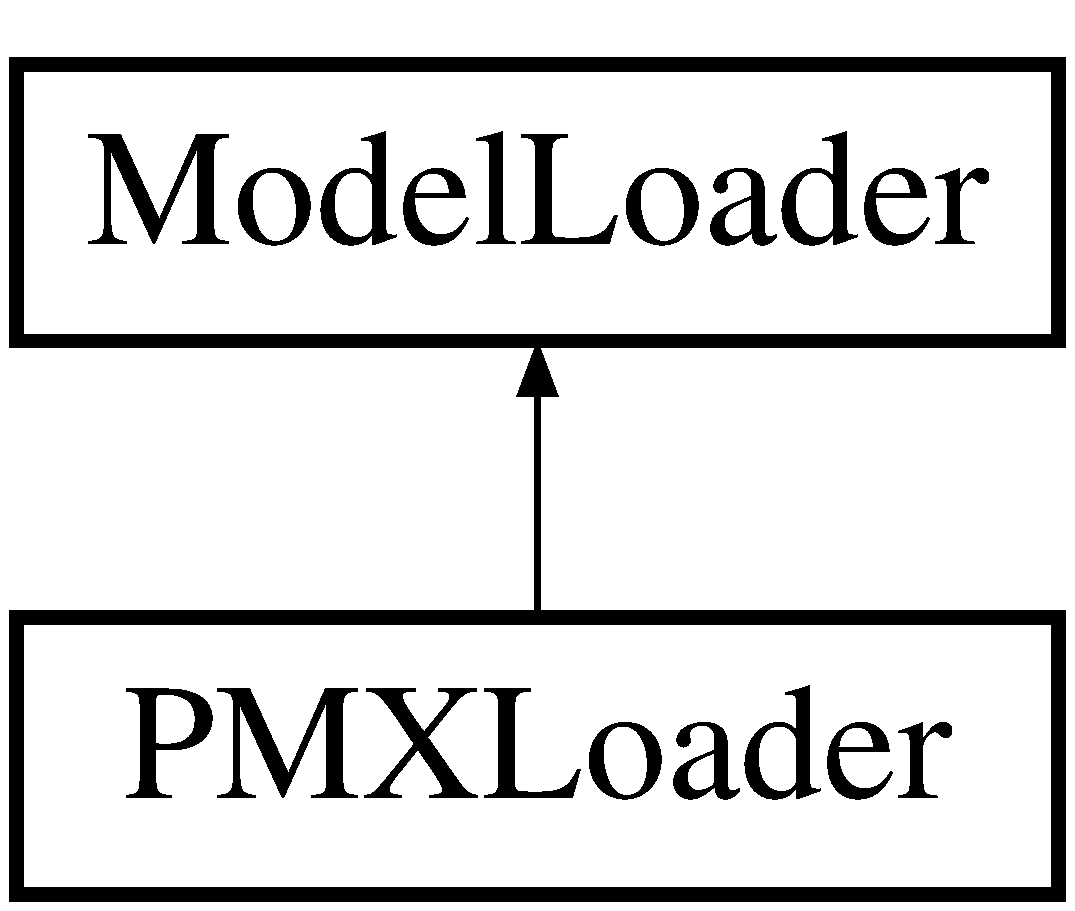
\includegraphics[height=2.000000cm]{class_p_m_x_loader}
\end{center}
\end{figure}
\subsection*{公開メンバ関数}
\begin{DoxyCompactItemize}
\item 
\mbox{\hyperlink{class_p_m_x_loader_aa8e1053ae62f8c36518ed0605a19ebd8}{P\+M\+X\+Loader}} (std\+::shared\+\_\+ptr$<$ \mbox{\hyperlink{class_device}{Device}} $>$ device)
\item 
\mbox{\hyperlink{class_p_m_x_loader_a35af7321f1d7cddb974da619eeea46cd}{$\sim$\+P\+M\+X\+Loader}} ()
\item 
std\+::shared\+\_\+ptr$<$ \mbox{\hyperlink{class_model}{Model}} $>$ \mbox{\hyperlink{class_p_m_x_loader_aee4e81ab65eeec5c9772ed5a8de6c5fa}{Load\+Model}} (const std\+::string \&file\+Path)
\item 
void \mbox{\hyperlink{class_p_m_x_loader_a1c4f3f379e18d6978b7684ab9d901952}{Clear\+Model\+Data}} ()
\end{DoxyCompactItemize}
\subsection*{静的公開メンバ関数}
\begin{DoxyCompactItemize}
\item 
static std\+::shared\+\_\+ptr$<$ \mbox{\hyperlink{class_p_m_x_loader}{P\+M\+X\+Loader}} $>$ \mbox{\hyperlink{class_p_m_x_loader_afc9fa9ff6b5010857102ed82fd441f1b}{Create}} (std\+::shared\+\_\+ptr$<$ \mbox{\hyperlink{class_device}{Device}} $>$ device)
\end{DoxyCompactItemize}
\subsection*{その他の継承メンバ}


\subsection{構築子と解体子}
\mbox{\Hypertarget{class_p_m_x_loader_aa8e1053ae62f8c36518ed0605a19ebd8}\label{class_p_m_x_loader_aa8e1053ae62f8c36518ed0605a19ebd8}} 
\index{P\+M\+X\+Loader@{P\+M\+X\+Loader}!P\+M\+X\+Loader@{P\+M\+X\+Loader}}
\index{P\+M\+X\+Loader@{P\+M\+X\+Loader}!P\+M\+X\+Loader@{P\+M\+X\+Loader}}
\subsubsection{\texorpdfstring{P\+M\+X\+Loader()}{PMXLoader()}}
{\footnotesize\ttfamily P\+M\+X\+Loader\+::\+P\+M\+X\+Loader (\begin{DoxyParamCaption}\item[{std\+::shared\+\_\+ptr$<$ \mbox{\hyperlink{class_device}{Device}} $>$}]{device }\end{DoxyParamCaption})}

\mbox{\Hypertarget{class_p_m_x_loader_a35af7321f1d7cddb974da619eeea46cd}\label{class_p_m_x_loader_a35af7321f1d7cddb974da619eeea46cd}} 
\index{P\+M\+X\+Loader@{P\+M\+X\+Loader}!````~P\+M\+X\+Loader@{$\sim$\+P\+M\+X\+Loader}}
\index{````~P\+M\+X\+Loader@{$\sim$\+P\+M\+X\+Loader}!P\+M\+X\+Loader@{P\+M\+X\+Loader}}
\subsubsection{\texorpdfstring{$\sim$\+P\+M\+X\+Loader()}{~PMXLoader()}}
{\footnotesize\ttfamily P\+M\+X\+Loader\+::$\sim$\+P\+M\+X\+Loader (\begin{DoxyParamCaption}{ }\end{DoxyParamCaption})}



\subsection{関数詳解}
\mbox{\Hypertarget{class_p_m_x_loader_a1c4f3f379e18d6978b7684ab9d901952}\label{class_p_m_x_loader_a1c4f3f379e18d6978b7684ab9d901952}} 
\index{P\+M\+X\+Loader@{P\+M\+X\+Loader}!Clear\+Model\+Data@{Clear\+Model\+Data}}
\index{Clear\+Model\+Data@{Clear\+Model\+Data}!P\+M\+X\+Loader@{P\+M\+X\+Loader}}
\subsubsection{\texorpdfstring{Clear\+Model\+Data()}{ClearModelData()}}
{\footnotesize\ttfamily void P\+M\+X\+Loader\+::\+Clear\+Model\+Data (\begin{DoxyParamCaption}{ }\end{DoxyParamCaption})\hspace{0.3cm}{\ttfamily [virtual]}}

読み込んだモデル情報を削除する 

\mbox{\hyperlink{class_model_loader_a6662edd78b17eeead09e822e19fc1799}{Model\+Loader}}を実装しています。

\mbox{\Hypertarget{class_p_m_x_loader_afc9fa9ff6b5010857102ed82fd441f1b}\label{class_p_m_x_loader_afc9fa9ff6b5010857102ed82fd441f1b}} 
\index{P\+M\+X\+Loader@{P\+M\+X\+Loader}!Create@{Create}}
\index{Create@{Create}!P\+M\+X\+Loader@{P\+M\+X\+Loader}}
\subsubsection{\texorpdfstring{Create()}{Create()}}
{\footnotesize\ttfamily std\+::shared\+\_\+ptr$<$ \mbox{\hyperlink{class_p_m_x_loader}{P\+M\+X\+Loader}} $>$ P\+M\+X\+Loader\+::\+Create (\begin{DoxyParamCaption}\item[{std\+::shared\+\_\+ptr$<$ \mbox{\hyperlink{class_device}{Device}} $>$}]{device }\end{DoxyParamCaption})\hspace{0.3cm}{\ttfamily [static]}}

\mbox{\Hypertarget{class_p_m_x_loader_aee4e81ab65eeec5c9772ed5a8de6c5fa}\label{class_p_m_x_loader_aee4e81ab65eeec5c9772ed5a8de6c5fa}} 
\index{P\+M\+X\+Loader@{P\+M\+X\+Loader}!Load\+Model@{Load\+Model}}
\index{Load\+Model@{Load\+Model}!P\+M\+X\+Loader@{P\+M\+X\+Loader}}
\subsubsection{\texorpdfstring{Load\+Model()}{LoadModel()}}
{\footnotesize\ttfamily std\+::shared\+\_\+ptr$<$ \mbox{\hyperlink{class_model}{Model}} $>$ P\+M\+X\+Loader\+::\+Load\+Model (\begin{DoxyParamCaption}\item[{const std\+::string \&}]{file\+Path }\end{DoxyParamCaption})\hspace{0.3cm}{\ttfamily [virtual]}}

モデルをロードする 
\begin{DoxyParams}[1]{引数}
\mbox{\tt in}  & {\em file\+Path} & \+: ファイルパス \\
\hline
\end{DoxyParams}


\mbox{\hyperlink{class_model_loader_a8e2157daa8d364c36fd26922f04adcb0}{Model\+Loader}}を実装しています。



このクラス詳解は次のファイルから抽出されました\+:\begin{DoxyCompactItemize}
\item 
Source/\+Model/\mbox{\hyperlink{_p_m_x_loader_8h}{P\+M\+X\+Loader.\+h}}\item 
Source/\+Model/\mbox{\hyperlink{_p_m_x_loader_8cpp}{P\+M\+X\+Loader.\+cpp}}\end{DoxyCompactItemize}

\hypertarget{class_p_m_x_model_data}{}\section{P\+M\+X\+Model\+Data クラス}
\label{class_p_m_x_model_data}\index{P\+M\+X\+Model\+Data@{P\+M\+X\+Model\+Data}}


{\ttfamily \#include $<$P\+M\+X\+Model\+Data.\+h$>$}

P\+M\+X\+Model\+Data の継承関係図\begin{figure}[H]
\begin{center}
\leavevmode
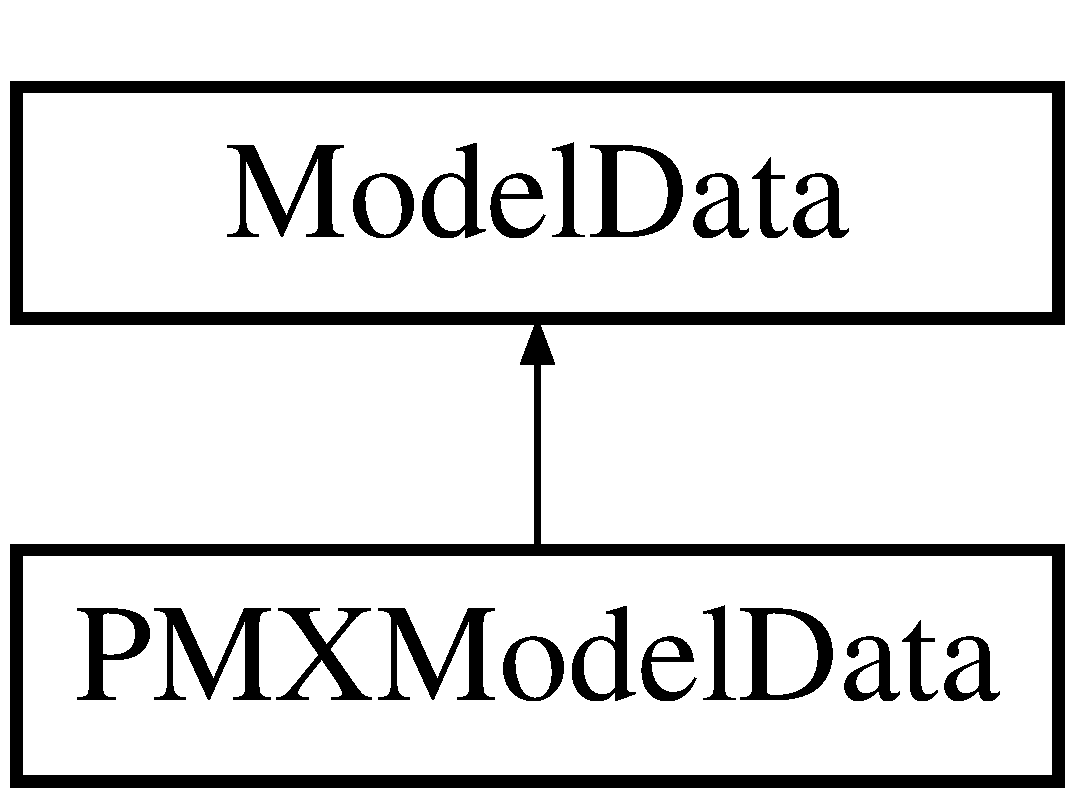
\includegraphics[height=2.000000cm]{class_p_m_x_model_data}
\end{center}
\end{figure}
\subsection*{公開メンバ関数}
\begin{DoxyCompactItemize}
\item 
\mbox{\hyperlink{class_p_m_x_model_data_a9865c076685f2efab59e2f19b12e86b5}{P\+M\+X\+Model\+Data}} (std\+::shared\+\_\+ptr$<$ \mbox{\hyperlink{class_device}{Device}} $>$ device, std\+::vector$<$ \mbox{\hyperlink{struct_p_m_x_1_1_vertex}{P\+M\+X\+::\+Vertex}} $>$ vertex\+Data, std\+::vector$<$ \mbox{\hyperlink{struct_p_m_x_1_1_index}{P\+M\+X\+::\+Index}} $>$ index\+Data, int material\+Count, int bone\+Count)
\item 
\mbox{\hyperlink{class_p_m_x_model_data_aab20c1e8dd3219cd165f877508e256a6}{$\sim$\+P\+M\+X\+Model\+Data}} ()
\item 
void \mbox{\hyperlink{class_p_m_x_model_data_a4c692007e0b890ee0bfd0f2bbbe0b97f}{Update}} ()
\item 
void \mbox{\hyperlink{class_p_m_x_model_data_aa88713736e3c337cabb23127c03be3c2}{Draw}} (Com\+Ptr$<$ I\+D3\+D12\+Graphics\+Command\+List $>$ graphics\+Command\+List, const \mbox{\hyperlink{struct_instance_data}{Instance\+Data}} \&instance\+Data) const
\end{DoxyCompactItemize}
\subsection*{静的公開メンバ関数}
\begin{DoxyCompactItemize}
\item 
static std\+::shared\+\_\+ptr$<$ \mbox{\hyperlink{class_p_m_x_model_data}{P\+M\+X\+Model\+Data}} $>$ \mbox{\hyperlink{class_p_m_x_model_data_a86aa963671719340a27fc76f88268dac}{Create}} (std\+::shared\+\_\+ptr$<$ \mbox{\hyperlink{class_device}{Device}} $>$ device, std\+::vector$<$ \mbox{\hyperlink{struct_p_m_x_1_1_vertex}{P\+M\+X\+::\+Vertex}} $>$ vertex\+Data, std\+::vector$<$ \mbox{\hyperlink{struct_p_m_x_1_1_index}{P\+M\+X\+::\+Index}} $>$ index\+Data)
\item 
static std\+::shared\+\_\+ptr$<$ \mbox{\hyperlink{class_p_m_x_model_data}{P\+M\+X\+Model\+Data}} $>$ \mbox{\hyperlink{class_p_m_x_model_data_ad65a359bdb1bd0e82225bee2c4158036}{Create}} (std\+::shared\+\_\+ptr$<$ \mbox{\hyperlink{class_device}{Device}} $>$ device, const \mbox{\hyperlink{struct_p_m_x_1_1_model_data_desc}{P\+M\+X\+::\+Model\+Data\+Desc}} \&model\+Data\+Desc)
\end{DoxyCompactItemize}
\subsection*{その他の継承メンバ}


\subsection{構築子と解体子}
\mbox{\Hypertarget{class_p_m_x_model_data_a9865c076685f2efab59e2f19b12e86b5}\label{class_p_m_x_model_data_a9865c076685f2efab59e2f19b12e86b5}} 
\index{P\+M\+X\+Model\+Data@{P\+M\+X\+Model\+Data}!P\+M\+X\+Model\+Data@{P\+M\+X\+Model\+Data}}
\index{P\+M\+X\+Model\+Data@{P\+M\+X\+Model\+Data}!P\+M\+X\+Model\+Data@{P\+M\+X\+Model\+Data}}
\subsubsection{\texorpdfstring{P\+M\+X\+Model\+Data()}{PMXModelData()}}
{\footnotesize\ttfamily P\+M\+X\+Model\+Data\+::\+P\+M\+X\+Model\+Data (\begin{DoxyParamCaption}\item[{std\+::shared\+\_\+ptr$<$ \mbox{\hyperlink{class_device}{Device}} $>$}]{device,  }\item[{std\+::vector$<$ \mbox{\hyperlink{struct_p_m_x_1_1_vertex}{P\+M\+X\+::\+Vertex}} $>$}]{vertex\+Data,  }\item[{std\+::vector$<$ \mbox{\hyperlink{struct_p_m_x_1_1_index}{P\+M\+X\+::\+Index}} $>$}]{index\+Data,  }\item[{int}]{material\+Count,  }\item[{int}]{bone\+Count }\end{DoxyParamCaption})}

\mbox{\Hypertarget{class_p_m_x_model_data_aab20c1e8dd3219cd165f877508e256a6}\label{class_p_m_x_model_data_aab20c1e8dd3219cd165f877508e256a6}} 
\index{P\+M\+X\+Model\+Data@{P\+M\+X\+Model\+Data}!````~P\+M\+X\+Model\+Data@{$\sim$\+P\+M\+X\+Model\+Data}}
\index{````~P\+M\+X\+Model\+Data@{$\sim$\+P\+M\+X\+Model\+Data}!P\+M\+X\+Model\+Data@{P\+M\+X\+Model\+Data}}
\subsubsection{\texorpdfstring{$\sim$\+P\+M\+X\+Model\+Data()}{~PMXModelData()}}
{\footnotesize\ttfamily P\+M\+X\+Model\+Data\+::$\sim$\+P\+M\+X\+Model\+Data (\begin{DoxyParamCaption}{ }\end{DoxyParamCaption})}



\subsection{関数詳解}
\mbox{\Hypertarget{class_p_m_x_model_data_a86aa963671719340a27fc76f88268dac}\label{class_p_m_x_model_data_a86aa963671719340a27fc76f88268dac}} 
\index{P\+M\+X\+Model\+Data@{P\+M\+X\+Model\+Data}!Create@{Create}}
\index{Create@{Create}!P\+M\+X\+Model\+Data@{P\+M\+X\+Model\+Data}}
\subsubsection{\texorpdfstring{Create()}{Create()}\hspace{0.1cm}{\footnotesize\ttfamily [1/2]}}
{\footnotesize\ttfamily std\+::shared\+\_\+ptr$<$ \mbox{\hyperlink{class_p_m_x_model_data}{P\+M\+X\+Model\+Data}} $>$ P\+M\+X\+Model\+Data\+::\+Create (\begin{DoxyParamCaption}\item[{std\+::shared\+\_\+ptr$<$ \mbox{\hyperlink{class_device}{Device}} $>$}]{device,  }\item[{std\+::vector$<$ \mbox{\hyperlink{struct_p_m_x_1_1_vertex}{P\+M\+X\+::\+Vertex}} $>$}]{vertex\+Data,  }\item[{std\+::vector$<$ \mbox{\hyperlink{struct_p_m_x_1_1_index}{P\+M\+X\+::\+Index}} $>$}]{index\+Data }\end{DoxyParamCaption})\hspace{0.3cm}{\ttfamily [static]}}

\mbox{\Hypertarget{class_p_m_x_model_data_ad65a359bdb1bd0e82225bee2c4158036}\label{class_p_m_x_model_data_ad65a359bdb1bd0e82225bee2c4158036}} 
\index{P\+M\+X\+Model\+Data@{P\+M\+X\+Model\+Data}!Create@{Create}}
\index{Create@{Create}!P\+M\+X\+Model\+Data@{P\+M\+X\+Model\+Data}}
\subsubsection{\texorpdfstring{Create()}{Create()}\hspace{0.1cm}{\footnotesize\ttfamily [2/2]}}
{\footnotesize\ttfamily std\+::shared\+\_\+ptr$<$ \mbox{\hyperlink{class_p_m_x_model_data}{P\+M\+X\+Model\+Data}} $>$ P\+M\+X\+Model\+Data\+::\+Create (\begin{DoxyParamCaption}\item[{std\+::shared\+\_\+ptr$<$ \mbox{\hyperlink{class_device}{Device}} $>$}]{device,  }\item[{const \mbox{\hyperlink{struct_p_m_x_1_1_model_data_desc}{P\+M\+X\+::\+Model\+Data\+Desc}} \&}]{model\+Data\+Desc }\end{DoxyParamCaption})\hspace{0.3cm}{\ttfamily [static]}}

\mbox{\Hypertarget{class_p_m_x_model_data_aa88713736e3c337cabb23127c03be3c2}\label{class_p_m_x_model_data_aa88713736e3c337cabb23127c03be3c2}} 
\index{P\+M\+X\+Model\+Data@{P\+M\+X\+Model\+Data}!Draw@{Draw}}
\index{Draw@{Draw}!P\+M\+X\+Model\+Data@{P\+M\+X\+Model\+Data}}
\subsubsection{\texorpdfstring{Draw()}{Draw()}}
{\footnotesize\ttfamily P\+M\+X\+Model\+Data\+::\+Draw (\begin{DoxyParamCaption}\item[{Com\+Ptr$<$ I\+D3\+D12\+Graphics\+Command\+List $>$}]{graphics\+Command\+List,  }\item[{const \mbox{\hyperlink{struct_instance_data}{Instance\+Data}} \&}]{instance\+Data }\end{DoxyParamCaption}) const\hspace{0.3cm}{\ttfamily [virtual]}}

描画処理 
\begin{DoxyParams}[1]{引数}
\mbox{\tt in}  & {\em graphics\+Command\+List} & \+: コマンドリスト \\
\hline
\mbox{\tt in}  & {\em instance\+Data} & \+: インスタンスデータ \\
\hline
\end{DoxyParams}


\mbox{\hyperlink{class_model_data_a774032c8dac7355ad2657c83cf0d1e21}{Model\+Data}}を再実装しています。

\mbox{\Hypertarget{class_p_m_x_model_data_a4c692007e0b890ee0bfd0f2bbbe0b97f}\label{class_p_m_x_model_data_a4c692007e0b890ee0bfd0f2bbbe0b97f}} 
\index{P\+M\+X\+Model\+Data@{P\+M\+X\+Model\+Data}!Update@{Update}}
\index{Update@{Update}!P\+M\+X\+Model\+Data@{P\+M\+X\+Model\+Data}}
\subsubsection{\texorpdfstring{Update()}{Update()}}
{\footnotesize\ttfamily P\+M\+X\+Model\+Data\+::\+Update (\begin{DoxyParamCaption}{ }\end{DoxyParamCaption})\hspace{0.3cm}{\ttfamily [virtual]}}

モデル情報の更新処理 

\mbox{\hyperlink{class_model_data_a67a18789221798611c63fd18edb3a9fc}{Model\+Data}}を再実装しています。



このクラス詳解は次のファイルから抽出されました\+:\begin{DoxyCompactItemize}
\item 
Source/\+Model/\mbox{\hyperlink{_p_m_x_model_data_8h}{P\+M\+X\+Model\+Data.\+h}}\item 
Source/\+Model/\mbox{\hyperlink{_p_m_x_model_data_8cpp}{P\+M\+X\+Model\+Data.\+cpp}}\end{DoxyCompactItemize}

\hypertarget{class_pose}{}\section{Pose クラス}
\label{class_pose}\index{Pose@{Pose}}


{\ttfamily \#include $<$Pose.\+h$>$}

\subsection*{公開メンバ関数}
\begin{DoxyCompactItemize}
\item 
\mbox{\hyperlink{class_pose_a4267a4b362912dded8377f2c3260803e}{$\sim$\+Pose}} ()
\begin{DoxyCompactList}\small\item\em デストラクタ \end{DoxyCompactList}\item 
void \mbox{\hyperlink{class_pose_a95523df0d97161fcf06258fa3dd556c7}{Calc\+Pose}} ()
\item 
const std\+::vector$<$ std\+::shared\+\_\+ptr$<$ \mbox{\hyperlink{class_bone}{Bone}} $>$ $>$ \& \mbox{\hyperlink{class_pose_a3767b292c049a75e996431649e246cc2}{Get\+Bones}} ()
\item 
bool \mbox{\hyperlink{class_pose_ae35ff02e01aac542188ad0ed885badfd}{Is\+Find\+Bone\+Name}} (const std\+::wstring \&bone\+Name)
\item 
int \mbox{\hyperlink{class_pose_a068da60cad6259e02fdc047a454b0cde}{Get\+Bone\+Index}} (const std\+::wstring \&bone\+Name)
\item 
void \mbox{\hyperlink{class_pose_ae64673fd020b5d6bc17dcac4607de85f}{Set\+Bone\+Data}} (const std\+::wstring \&bone\+Name, const std\+::shared\+\_\+ptr$<$ \mbox{\hyperlink{class_bone}{Bone}} $>$ bone, int bone\+Index, int parent\+Bone\+Index=-\/1)
\end{DoxyCompactItemize}
\subsection*{静的公開メンバ関数}
\begin{DoxyCompactItemize}
\item 
static std\+::shared\+\_\+ptr$<$ \mbox{\hyperlink{class_pose}{Pose}} $>$ \mbox{\hyperlink{class_pose_a47091fb8b00829db53ec72d7f35a1cad}{Create}} (int bone\+Count)
\item 
static std\+::shared\+\_\+ptr$<$ \mbox{\hyperlink{class_pose}{Pose}} $>$ \mbox{\hyperlink{class_pose_a44d938544c9613f1753007fa2e419bdd}{Create}} (std\+::shared\+\_\+ptr$<$ \mbox{\hyperlink{class_pose}{Pose}} $>$ default\+Pose)
\item 
static std\+::shared\+\_\+ptr$<$ \mbox{\hyperlink{class_pose}{Pose}} $>$ \mbox{\hyperlink{class_pose_a250f6075206d81cde427646d72e75ec5}{Lerp}} (const std\+::shared\+\_\+ptr$<$ \mbox{\hyperlink{class_pose}{Pose}} $>$ pre\+Pose, const std\+::shared\+\_\+ptr$<$ \mbox{\hyperlink{class_pose}{Pose}} $>$ post\+Pose, float time)
\end{DoxyCompactItemize}


\subsection{構築子と解体子}
\mbox{\Hypertarget{class_pose_a4267a4b362912dded8377f2c3260803e}\label{class_pose_a4267a4b362912dded8377f2c3260803e}} 
\index{Pose@{Pose}!````~Pose@{$\sim$\+Pose}}
\index{````~Pose@{$\sim$\+Pose}!Pose@{Pose}}
\subsubsection{\texorpdfstring{$\sim$\+Pose()}{~Pose()}}
{\footnotesize\ttfamily Pose\+::$\sim$\+Pose (\begin{DoxyParamCaption}{ }\end{DoxyParamCaption})}



デストラクタ 



\subsection{関数詳解}
\mbox{\Hypertarget{class_pose_a95523df0d97161fcf06258fa3dd556c7}\label{class_pose_a95523df0d97161fcf06258fa3dd556c7}} 
\index{Pose@{Pose}!Calc\+Pose@{Calc\+Pose}}
\index{Calc\+Pose@{Calc\+Pose}!Pose@{Pose}}
\subsubsection{\texorpdfstring{Calc\+Pose()}{CalcPose()}}
{\footnotesize\ttfamily Pose\+::\+Calc\+Pose (\begin{DoxyParamCaption}{ }\end{DoxyParamCaption})}

姿勢計算を行う \mbox{\Hypertarget{class_pose_a47091fb8b00829db53ec72d7f35a1cad}\label{class_pose_a47091fb8b00829db53ec72d7f35a1cad}} 
\index{Pose@{Pose}!Create@{Create}}
\index{Create@{Create}!Pose@{Pose}}
\subsubsection{\texorpdfstring{Create()}{Create()}\hspace{0.1cm}{\footnotesize\ttfamily [1/2]}}
{\footnotesize\ttfamily std\+::shared\+\_\+ptr$<$ \mbox{\hyperlink{class_pose}{Pose}} $>$ Pose\+::\+Create (\begin{DoxyParamCaption}\item[{int}]{bone\+Count }\end{DoxyParamCaption})\hspace{0.3cm}{\ttfamily [static]}}

\mbox{\Hypertarget{class_pose_a44d938544c9613f1753007fa2e419bdd}\label{class_pose_a44d938544c9613f1753007fa2e419bdd}} 
\index{Pose@{Pose}!Create@{Create}}
\index{Create@{Create}!Pose@{Pose}}
\subsubsection{\texorpdfstring{Create()}{Create()}\hspace{0.1cm}{\footnotesize\ttfamily [2/2]}}
{\footnotesize\ttfamily std\+::shared\+\_\+ptr$<$ \mbox{\hyperlink{class_pose}{Pose}} $>$ Pose\+::\+Create (\begin{DoxyParamCaption}\item[{std\+::shared\+\_\+ptr$<$ \mbox{\hyperlink{class_pose}{Pose}} $>$}]{default\+Pose }\end{DoxyParamCaption})\hspace{0.3cm}{\ttfamily [static]}}

\mbox{\Hypertarget{class_pose_a068da60cad6259e02fdc047a454b0cde}\label{class_pose_a068da60cad6259e02fdc047a454b0cde}} 
\index{Pose@{Pose}!Get\+Bone\+Index@{Get\+Bone\+Index}}
\index{Get\+Bone\+Index@{Get\+Bone\+Index}!Pose@{Pose}}
\subsubsection{\texorpdfstring{Get\+Bone\+Index()}{GetBoneIndex()}}
{\footnotesize\ttfamily Pose\+::\+Get\+Bone\+Index (\begin{DoxyParamCaption}\item[{const std\+::wstring \&}]{bone\+Name }\end{DoxyParamCaption})}

ボーン名からボーンのインデックスを取得する 
\begin{DoxyParams}[1]{引数}
\mbox{\tt in}  & {\em bone\+Name} & \+: ボーン名 \\
\hline
\end{DoxyParams}

\begin{DoxyRetVals}{戻り値}
{\em ボーンのインデックス} & \\
\hline
\end{DoxyRetVals}
\begin{DoxyNote}{覚え書き}
指定したボーンが存在するかを Is\+Find\+Bone\+Nameで事前にチェックする必要あり 
\end{DoxyNote}
\mbox{\Hypertarget{class_pose_a3767b292c049a75e996431649e246cc2}\label{class_pose_a3767b292c049a75e996431649e246cc2}} 
\index{Pose@{Pose}!Get\+Bones@{Get\+Bones}}
\index{Get\+Bones@{Get\+Bones}!Pose@{Pose}}
\subsubsection{\texorpdfstring{Get\+Bones()}{GetBones()}}
{\footnotesize\ttfamily Pose\+::\+Get\+Bones (\begin{DoxyParamCaption}{ }\end{DoxyParamCaption})}

ボーン配列を取得する 
\begin{DoxyRetVals}{戻り値}
{\em ボーン配列の参照} & \\
\hline
\end{DoxyRetVals}
\mbox{\Hypertarget{class_pose_ae35ff02e01aac542188ad0ed885badfd}\label{class_pose_ae35ff02e01aac542188ad0ed885badfd}} 
\index{Pose@{Pose}!Is\+Find\+Bone\+Name@{Is\+Find\+Bone\+Name}}
\index{Is\+Find\+Bone\+Name@{Is\+Find\+Bone\+Name}!Pose@{Pose}}
\subsubsection{\texorpdfstring{Is\+Find\+Bone\+Name()}{IsFindBoneName()}}
{\footnotesize\ttfamily Pose\+::\+Is\+Find\+Bone\+Name (\begin{DoxyParamCaption}\item[{const std\+::wstring \&}]{bone\+Name }\end{DoxyParamCaption})}

指定した名前のボーンが存在するかチェックする 
\begin{DoxyParams}[1]{引数}
\mbox{\tt in}  & {\em ボーン名} & \\
\hline
\end{DoxyParams}

\begin{DoxyRetVals}{戻り値}
{\em ボーンが存在する} & \+: true \\
\hline
{\em ボーンが存在しない} & \+: false \\
\hline
\end{DoxyRetVals}
\mbox{\Hypertarget{class_pose_a250f6075206d81cde427646d72e75ec5}\label{class_pose_a250f6075206d81cde427646d72e75ec5}} 
\index{Pose@{Pose}!Lerp@{Lerp}}
\index{Lerp@{Lerp}!Pose@{Pose}}
\subsubsection{\texorpdfstring{Lerp()}{Lerp()}}
{\footnotesize\ttfamily Pose\+::\+Lerp (\begin{DoxyParamCaption}\item[{const std\+::shared\+\_\+ptr$<$ \mbox{\hyperlink{class_pose}{Pose}} $>$}]{pre\+Pose,  }\item[{const std\+::shared\+\_\+ptr$<$ \mbox{\hyperlink{class_pose}{Pose}} $>$}]{post\+Pose,  }\item[{float}]{time }\end{DoxyParamCaption})\hspace{0.3cm}{\ttfamily [static]}}

姿勢情報を補間する 
\begin{DoxyParams}[1]{引数}
\mbox{\tt in}  & {\em pre\+Pose} & \+: time = 0.\+0 の場合の姿勢 \\
\hline
\mbox{\tt in}  & {\em post\+Pose} & \+: time = 1.\+0 の場合の姿勢 \\
\hline
\mbox{\tt in}  & {\em time} & \+: 補間係数( 0.\+0 $<$= time $<$= 1.\+0 にクランプされる ) \\
\hline
\end{DoxyParams}

\begin{DoxyRetVals}{戻り値}
{\em 姿勢行列計算前の姿勢} & \\
\hline
\end{DoxyRetVals}
\mbox{\Hypertarget{class_pose_ae64673fd020b5d6bc17dcac4607de85f}\label{class_pose_ae64673fd020b5d6bc17dcac4607de85f}} 
\index{Pose@{Pose}!Set\+Bone\+Data@{Set\+Bone\+Data}}
\index{Set\+Bone\+Data@{Set\+Bone\+Data}!Pose@{Pose}}
\subsubsection{\texorpdfstring{Set\+Bone\+Data()}{SetBoneData()}}
{\footnotesize\ttfamily Pose\+::\+Set\+Bone\+Data (\begin{DoxyParamCaption}\item[{const std\+::wstring \&}]{bone\+Name,  }\item[{const std\+::shared\+\_\+ptr$<$ \mbox{\hyperlink{class_bone}{Bone}} $>$}]{bone,  }\item[{int}]{bone\+Index,  }\item[{int}]{parent\+Bone\+Index = {\ttfamily -\/1} }\end{DoxyParamCaption})}

ボーン情報を追加する 
\begin{DoxyParams}[1]{引数}
\mbox{\tt in}  & {\em bone\+Name} & ボーン名 \\
\hline
\mbox{\tt in}  & {\em bone} & \+: ボーン情報 \\
\hline
\mbox{\tt in}  & {\em bone\+Index} & \+: 自身のインデックス \\
\hline
\mbox{\tt in}  & {\em parent\+Bone\+Index} & \+: 親のインデックス \\
\hline
\end{DoxyParams}
\begin{DoxyNote}{覚え書き}
すべての親ノードは-\/1とし、親ノードに接続されていないボーンは 姿勢計算対象外になる 
\end{DoxyNote}


このクラス詳解は次のファイルから抽出されました\+:\begin{DoxyCompactItemize}
\item 
Source/\mbox{\hyperlink{_pose_8h}{Pose.\+h}}\item 
Source/\mbox{\hyperlink{_pose_8cpp}{Pose.\+cpp}}\end{DoxyCompactItemize}

\hypertarget{struct_math_1_1_quaternion}{}\section{Math\+:\+:Quaternion 構造体}
\label{struct_math_1_1_quaternion}\index{Math\+::\+Quaternion@{Math\+::\+Quaternion}}


{\ttfamily \#include $<$Math.\+h$>$}

\subsection*{公開メンバ関数}
\begin{DoxyCompactItemize}
\item 
\mbox{\hyperlink{struct_math_1_1_quaternion_abcc01358aada56ea5f0db4da18aaf77d}{Quaternion}} ()
\item 
\mbox{\hyperlink{struct_math_1_1_quaternion_a36beaf9a73a54a368217dde43aa81cb0}{Quaternion}} (float mw, float mx, float my, float mz)
\item 
\mbox{\hyperlink{struct_math_1_1_quaternion_abe837b2cab65532540a3f8ca9a171c71}{Quaternion}} (float mx, float my, float mz)
\item 
\mbox{\hyperlink{struct_math_1_1_quaternion_aee457d8f04d226335213714897d752dd}{Quaternion}} (const \mbox{\hyperlink{struct_math_1_1_vector3}{Math\+::\+Vector3}} \&vector)
\item 
\mbox{\hyperlink{struct_math_1_1_quaternion_acae9b6b6548813cbcbd1f5b641e4f064}{Quaternion}} (const \mbox{\hyperlink{struct_math_1_1_quaternion}{Quaternion}} \&other)
\item 
\mbox{\hyperlink{struct_math_1_1_quaternion_a68ab22588ee547c1b03c58f717b5f838}{Quaternion}} (\mbox{\hyperlink{struct_math_1_1_quaternion}{Quaternion}} \&\&other)
\item 
\mbox{\hyperlink{struct_math_1_1_quaternion}{Quaternion}} \mbox{\hyperlink{struct_math_1_1_quaternion_aa22c281886948b07c70b35e0de42dc39}{operator+}} () const
\item 
\mbox{\hyperlink{struct_math_1_1_quaternion}{Quaternion}} \mbox{\hyperlink{struct_math_1_1_quaternion_aff7a0a5aeea4a3fe860cb90a649e389c}{operator-\/}} () const
\item 
\mbox{\hyperlink{struct_math_1_1_quaternion}{Quaternion}} \& \mbox{\hyperlink{struct_math_1_1_quaternion_acb64d4da834f6bc8f2cdcbd5525c05d4}{operator=}} (const \mbox{\hyperlink{struct_math_1_1_quaternion}{Quaternion}} \&quat)
\item 
\mbox{\hyperlink{struct_math_1_1_quaternion}{Quaternion}} \& \mbox{\hyperlink{struct_math_1_1_quaternion_a089bf5e8aa4d7441b364f2b7f34a64ac}{operator+=}} (const \mbox{\hyperlink{struct_math_1_1_quaternion}{Quaternion}} \&quat)
\item 
\mbox{\hyperlink{struct_math_1_1_quaternion}{Quaternion}} \& \mbox{\hyperlink{struct_math_1_1_quaternion_af1884a86f9d7d61197a2fb8a704bc58f}{operator-\/=}} (const \mbox{\hyperlink{struct_math_1_1_quaternion}{Quaternion}} \&quat)
\item 
\mbox{\hyperlink{struct_math_1_1_quaternion}{Quaternion}} \& \mbox{\hyperlink{struct_math_1_1_quaternion_ab259c5d0a79c9fcb816b2167f8dc32dd}{operator$\ast$=}} (const \mbox{\hyperlink{struct_math_1_1_quaternion}{Quaternion}} \&quat)
\item 
\mbox{\hyperlink{struct_math_1_1_quaternion}{Quaternion}} \& \mbox{\hyperlink{struct_math_1_1_quaternion_a138f8b4c70cf0280ad19072c675201ab}{operator$\ast$=}} (float scale)
\item 
\mbox{\hyperlink{struct_math_1_1_quaternion}{Quaternion}} \& \mbox{\hyperlink{struct_math_1_1_quaternion_a04a144dcc8a5401104fd88248b13e84a}{operator/=}} (const \mbox{\hyperlink{struct_math_1_1_quaternion}{Quaternion}} \&quat)
\item 
\mbox{\hyperlink{struct_math_1_1_quaternion}{Quaternion}} \& \mbox{\hyperlink{struct_math_1_1_quaternion_a2157dd9798f538ebd2463cd962c11a64}{operator/=}} (float scale)
\item 
float \mbox{\hyperlink{struct_math_1_1_quaternion_a1cd5a9d8be7f9b85c4eb7ba661238a09}{Norm}} () const
\item 
float \mbox{\hyperlink{struct_math_1_1_quaternion_a8f147b15819df35d4448c9765adc4eb8}{Norm\+Square}} () const
\end{DoxyCompactItemize}
\subsection*{公開変数類}
\begin{DoxyCompactItemize}
\item 
\begin{tabbing}
xx\=xx\=xx\=xx\=xx\=xx\=xx\=xx\=xx\=\kill
union \{\\
\>struct \{\\
\>\>float \mbox{\hyperlink{struct_math_1_1_quaternion_ad482a0bc0b3759696ce73af10ae4ce62}{x}}\\
\>\>float \mbox{\hyperlink{struct_math_1_1_quaternion_affec7ef4764711e8df983d5439494050}{y}}\\
\>\>float \mbox{\hyperlink{struct_math_1_1_quaternion_af5df1935c0d63acfd4fc4e65ae0e30d2}{z}}\\
\>\} \\
\>\mbox{\hyperlink{struct_math_1_1_vector3}{Vector3}} \mbox{\hyperlink{struct_math_1_1_quaternion_a628a90b817e19edde055fc4745e25f5c}{v}}\\
\}; \\

\end{tabbing}\item 
float \mbox{\hyperlink{struct_math_1_1_quaternion_a9736171bbae3bee22f12d23f3fefb682}{w}}
\end{DoxyCompactItemize}


\subsection{構築子と解体子}
\mbox{\Hypertarget{struct_math_1_1_quaternion_abcc01358aada56ea5f0db4da18aaf77d}\label{struct_math_1_1_quaternion_abcc01358aada56ea5f0db4da18aaf77d}} 
\index{Math\+::\+Quaternion@{Math\+::\+Quaternion}!Quaternion@{Quaternion}}
\index{Quaternion@{Quaternion}!Math\+::\+Quaternion@{Math\+::\+Quaternion}}
\subsubsection{\texorpdfstring{Quaternion()}{Quaternion()}\hspace{0.1cm}{\footnotesize\ttfamily [1/6]}}
{\footnotesize\ttfamily Quaternion\+::\+Quaternion (\begin{DoxyParamCaption}{ }\end{DoxyParamCaption})}

\mbox{\Hypertarget{struct_math_1_1_quaternion_a36beaf9a73a54a368217dde43aa81cb0}\label{struct_math_1_1_quaternion_a36beaf9a73a54a368217dde43aa81cb0}} 
\index{Math\+::\+Quaternion@{Math\+::\+Quaternion}!Quaternion@{Quaternion}}
\index{Quaternion@{Quaternion}!Math\+::\+Quaternion@{Math\+::\+Quaternion}}
\subsubsection{\texorpdfstring{Quaternion()}{Quaternion()}\hspace{0.1cm}{\footnotesize\ttfamily [2/6]}}
{\footnotesize\ttfamily Quaternion\+::\+Quaternion (\begin{DoxyParamCaption}\item[{float}]{mw,  }\item[{float}]{mx,  }\item[{float}]{my,  }\item[{float}]{mz }\end{DoxyParamCaption})}

\mbox{\Hypertarget{struct_math_1_1_quaternion_abe837b2cab65532540a3f8ca9a171c71}\label{struct_math_1_1_quaternion_abe837b2cab65532540a3f8ca9a171c71}} 
\index{Math\+::\+Quaternion@{Math\+::\+Quaternion}!Quaternion@{Quaternion}}
\index{Quaternion@{Quaternion}!Math\+::\+Quaternion@{Math\+::\+Quaternion}}
\subsubsection{\texorpdfstring{Quaternion()}{Quaternion()}\hspace{0.1cm}{\footnotesize\ttfamily [3/6]}}
{\footnotesize\ttfamily Quaternion\+::\+Quaternion (\begin{DoxyParamCaption}\item[{float}]{mx,  }\item[{float}]{my,  }\item[{float}]{mz }\end{DoxyParamCaption})}

\mbox{\Hypertarget{struct_math_1_1_quaternion_aee457d8f04d226335213714897d752dd}\label{struct_math_1_1_quaternion_aee457d8f04d226335213714897d752dd}} 
\index{Math\+::\+Quaternion@{Math\+::\+Quaternion}!Quaternion@{Quaternion}}
\index{Quaternion@{Quaternion}!Math\+::\+Quaternion@{Math\+::\+Quaternion}}
\subsubsection{\texorpdfstring{Quaternion()}{Quaternion()}\hspace{0.1cm}{\footnotesize\ttfamily [4/6]}}
{\footnotesize\ttfamily Math\+::\+Quaternion\+::\+Quaternion (\begin{DoxyParamCaption}\item[{const \mbox{\hyperlink{struct_math_1_1_vector3}{Math\+::\+Vector3}} \&}]{vector }\end{DoxyParamCaption})}

\mbox{\Hypertarget{struct_math_1_1_quaternion_acae9b6b6548813cbcbd1f5b641e4f064}\label{struct_math_1_1_quaternion_acae9b6b6548813cbcbd1f5b641e4f064}} 
\index{Math\+::\+Quaternion@{Math\+::\+Quaternion}!Quaternion@{Quaternion}}
\index{Quaternion@{Quaternion}!Math\+::\+Quaternion@{Math\+::\+Quaternion}}
\subsubsection{\texorpdfstring{Quaternion()}{Quaternion()}\hspace{0.1cm}{\footnotesize\ttfamily [5/6]}}
{\footnotesize\ttfamily Quaternion\+::\+Quaternion (\begin{DoxyParamCaption}\item[{const \mbox{\hyperlink{struct_math_1_1_quaternion}{Quaternion}} \&}]{other }\end{DoxyParamCaption})}

\mbox{\Hypertarget{struct_math_1_1_quaternion_a68ab22588ee547c1b03c58f717b5f838}\label{struct_math_1_1_quaternion_a68ab22588ee547c1b03c58f717b5f838}} 
\index{Math\+::\+Quaternion@{Math\+::\+Quaternion}!Quaternion@{Quaternion}}
\index{Quaternion@{Quaternion}!Math\+::\+Quaternion@{Math\+::\+Quaternion}}
\subsubsection{\texorpdfstring{Quaternion()}{Quaternion()}\hspace{0.1cm}{\footnotesize\ttfamily [6/6]}}
{\footnotesize\ttfamily Quaternion\+::\+Quaternion (\begin{DoxyParamCaption}\item[{\mbox{\hyperlink{struct_math_1_1_quaternion}{Quaternion}} \&\&}]{other }\end{DoxyParamCaption})}



\subsection{関数詳解}
\mbox{\Hypertarget{struct_math_1_1_quaternion_a1cd5a9d8be7f9b85c4eb7ba661238a09}\label{struct_math_1_1_quaternion_a1cd5a9d8be7f9b85c4eb7ba661238a09}} 
\index{Math\+::\+Quaternion@{Math\+::\+Quaternion}!Norm@{Norm}}
\index{Norm@{Norm}!Math\+::\+Quaternion@{Math\+::\+Quaternion}}
\subsubsection{\texorpdfstring{Norm()}{Norm()}}
{\footnotesize\ttfamily float Math\+::\+Quaternion\+::\+Norm (\begin{DoxyParamCaption}{ }\end{DoxyParamCaption}) const}

\mbox{\Hypertarget{struct_math_1_1_quaternion_a8f147b15819df35d4448c9765adc4eb8}\label{struct_math_1_1_quaternion_a8f147b15819df35d4448c9765adc4eb8}} 
\index{Math\+::\+Quaternion@{Math\+::\+Quaternion}!Norm\+Square@{Norm\+Square}}
\index{Norm\+Square@{Norm\+Square}!Math\+::\+Quaternion@{Math\+::\+Quaternion}}
\subsubsection{\texorpdfstring{Norm\+Square()}{NormSquare()}}
{\footnotesize\ttfamily float Math\+::\+Quaternion\+::\+Norm\+Square (\begin{DoxyParamCaption}{ }\end{DoxyParamCaption}) const}

\mbox{\Hypertarget{struct_math_1_1_quaternion_ab259c5d0a79c9fcb816b2167f8dc32dd}\label{struct_math_1_1_quaternion_ab259c5d0a79c9fcb816b2167f8dc32dd}} 
\index{Math\+::\+Quaternion@{Math\+::\+Quaternion}!operator$\ast$=@{operator$\ast$=}}
\index{operator$\ast$=@{operator$\ast$=}!Math\+::\+Quaternion@{Math\+::\+Quaternion}}
\subsubsection{\texorpdfstring{operator$\ast$=()}{operator*=()}\hspace{0.1cm}{\footnotesize\ttfamily [1/2]}}
{\footnotesize\ttfamily \mbox{\hyperlink{struct_math_1_1_quaternion}{Quaternion}} \& Quaternion\+::operator$\ast$= (\begin{DoxyParamCaption}\item[{const \mbox{\hyperlink{struct_math_1_1_quaternion}{Quaternion}} \&}]{quat }\end{DoxyParamCaption})}

\mbox{\Hypertarget{struct_math_1_1_quaternion_a138f8b4c70cf0280ad19072c675201ab}\label{struct_math_1_1_quaternion_a138f8b4c70cf0280ad19072c675201ab}} 
\index{Math\+::\+Quaternion@{Math\+::\+Quaternion}!operator$\ast$=@{operator$\ast$=}}
\index{operator$\ast$=@{operator$\ast$=}!Math\+::\+Quaternion@{Math\+::\+Quaternion}}
\subsubsection{\texorpdfstring{operator$\ast$=()}{operator*=()}\hspace{0.1cm}{\footnotesize\ttfamily [2/2]}}
{\footnotesize\ttfamily \mbox{\hyperlink{struct_math_1_1_quaternion}{Quaternion}} \& Math\+::\+Quaternion\+::operator$\ast$= (\begin{DoxyParamCaption}\item[{float}]{scale }\end{DoxyParamCaption})}

\mbox{\Hypertarget{struct_math_1_1_quaternion_aa22c281886948b07c70b35e0de42dc39}\label{struct_math_1_1_quaternion_aa22c281886948b07c70b35e0de42dc39}} 
\index{Math\+::\+Quaternion@{Math\+::\+Quaternion}!operator+@{operator+}}
\index{operator+@{operator+}!Math\+::\+Quaternion@{Math\+::\+Quaternion}}
\subsubsection{\texorpdfstring{operator+()}{operator+()}}
{\footnotesize\ttfamily \mbox{\hyperlink{struct_math_1_1_quaternion}{Quaternion}} Quaternion\+::operator+ (\begin{DoxyParamCaption}{ }\end{DoxyParamCaption}) const}

\mbox{\Hypertarget{struct_math_1_1_quaternion_a089bf5e8aa4d7441b364f2b7f34a64ac}\label{struct_math_1_1_quaternion_a089bf5e8aa4d7441b364f2b7f34a64ac}} 
\index{Math\+::\+Quaternion@{Math\+::\+Quaternion}!operator+=@{operator+=}}
\index{operator+=@{operator+=}!Math\+::\+Quaternion@{Math\+::\+Quaternion}}
\subsubsection{\texorpdfstring{operator+=()}{operator+=()}}
{\footnotesize\ttfamily \mbox{\hyperlink{struct_math_1_1_quaternion}{Quaternion}} \& Quaternion\+::operator+= (\begin{DoxyParamCaption}\item[{const \mbox{\hyperlink{struct_math_1_1_quaternion}{Quaternion}} \&}]{quat }\end{DoxyParamCaption})}

\mbox{\Hypertarget{struct_math_1_1_quaternion_aff7a0a5aeea4a3fe860cb90a649e389c}\label{struct_math_1_1_quaternion_aff7a0a5aeea4a3fe860cb90a649e389c}} 
\index{Math\+::\+Quaternion@{Math\+::\+Quaternion}!operator-\/@{operator-\/}}
\index{operator-\/@{operator-\/}!Math\+::\+Quaternion@{Math\+::\+Quaternion}}
\subsubsection{\texorpdfstring{operator-\/()}{operator-()}}
{\footnotesize\ttfamily \mbox{\hyperlink{struct_math_1_1_quaternion}{Quaternion}} Quaternion\+::operator-\/ (\begin{DoxyParamCaption}{ }\end{DoxyParamCaption}) const}

\mbox{\Hypertarget{struct_math_1_1_quaternion_af1884a86f9d7d61197a2fb8a704bc58f}\label{struct_math_1_1_quaternion_af1884a86f9d7d61197a2fb8a704bc58f}} 
\index{Math\+::\+Quaternion@{Math\+::\+Quaternion}!operator-\/=@{operator-\/=}}
\index{operator-\/=@{operator-\/=}!Math\+::\+Quaternion@{Math\+::\+Quaternion}}
\subsubsection{\texorpdfstring{operator-\/=()}{operator-=()}}
{\footnotesize\ttfamily \mbox{\hyperlink{struct_math_1_1_quaternion}{Quaternion}} \& Quaternion\+::operator-\/= (\begin{DoxyParamCaption}\item[{const \mbox{\hyperlink{struct_math_1_1_quaternion}{Quaternion}} \&}]{quat }\end{DoxyParamCaption})}

\mbox{\Hypertarget{struct_math_1_1_quaternion_a04a144dcc8a5401104fd88248b13e84a}\label{struct_math_1_1_quaternion_a04a144dcc8a5401104fd88248b13e84a}} 
\index{Math\+::\+Quaternion@{Math\+::\+Quaternion}!operator/=@{operator/=}}
\index{operator/=@{operator/=}!Math\+::\+Quaternion@{Math\+::\+Quaternion}}
\subsubsection{\texorpdfstring{operator/=()}{operator/=()}\hspace{0.1cm}{\footnotesize\ttfamily [1/2]}}
{\footnotesize\ttfamily \mbox{\hyperlink{struct_math_1_1_quaternion}{Quaternion}} \& Math\+::\+Quaternion\+::operator/= (\begin{DoxyParamCaption}\item[{const \mbox{\hyperlink{struct_math_1_1_quaternion}{Quaternion}} \&}]{quat }\end{DoxyParamCaption})}

\mbox{\Hypertarget{struct_math_1_1_quaternion_a2157dd9798f538ebd2463cd962c11a64}\label{struct_math_1_1_quaternion_a2157dd9798f538ebd2463cd962c11a64}} 
\index{Math\+::\+Quaternion@{Math\+::\+Quaternion}!operator/=@{operator/=}}
\index{operator/=@{operator/=}!Math\+::\+Quaternion@{Math\+::\+Quaternion}}
\subsubsection{\texorpdfstring{operator/=()}{operator/=()}\hspace{0.1cm}{\footnotesize\ttfamily [2/2]}}
{\footnotesize\ttfamily \mbox{\hyperlink{struct_math_1_1_quaternion}{Quaternion}} \& Math\+::\+Quaternion\+::operator/= (\begin{DoxyParamCaption}\item[{float}]{scale }\end{DoxyParamCaption})}

\mbox{\Hypertarget{struct_math_1_1_quaternion_acb64d4da834f6bc8f2cdcbd5525c05d4}\label{struct_math_1_1_quaternion_acb64d4da834f6bc8f2cdcbd5525c05d4}} 
\index{Math\+::\+Quaternion@{Math\+::\+Quaternion}!operator=@{operator=}}
\index{operator=@{operator=}!Math\+::\+Quaternion@{Math\+::\+Quaternion}}
\subsubsection{\texorpdfstring{operator=()}{operator=()}}
{\footnotesize\ttfamily \mbox{\hyperlink{struct_math_1_1_quaternion}{Quaternion}} \& Quaternion\+::operator= (\begin{DoxyParamCaption}\item[{const \mbox{\hyperlink{struct_math_1_1_quaternion}{Quaternion}} \&}]{quat }\end{DoxyParamCaption})}



\subsection{メンバ詳解}
\mbox{\Hypertarget{struct_math_1_1_quaternion_a09449d4fc06ef23c17f363910edf0c5a}\label{struct_math_1_1_quaternion_a09449d4fc06ef23c17f363910edf0c5a}} 
\subsubsection{\texorpdfstring{"@9}{@9}}
{\footnotesize\ttfamily union \{ ... \} }

\mbox{\Hypertarget{struct_math_1_1_quaternion_a628a90b817e19edde055fc4745e25f5c}\label{struct_math_1_1_quaternion_a628a90b817e19edde055fc4745e25f5c}} 
\index{Math\+::\+Quaternion@{Math\+::\+Quaternion}!v@{v}}
\index{v@{v}!Math\+::\+Quaternion@{Math\+::\+Quaternion}}
\subsubsection{\texorpdfstring{v}{v}}
{\footnotesize\ttfamily \mbox{\hyperlink{struct_math_1_1_vector3}{Vector3}} Math\+::\+Quaternion\+::v}

\mbox{\Hypertarget{struct_math_1_1_quaternion_a9736171bbae3bee22f12d23f3fefb682}\label{struct_math_1_1_quaternion_a9736171bbae3bee22f12d23f3fefb682}} 
\index{Math\+::\+Quaternion@{Math\+::\+Quaternion}!w@{w}}
\index{w@{w}!Math\+::\+Quaternion@{Math\+::\+Quaternion}}
\subsubsection{\texorpdfstring{w}{w}}
{\footnotesize\ttfamily float Math\+::\+Quaternion\+::w}

\mbox{\Hypertarget{struct_math_1_1_quaternion_ad482a0bc0b3759696ce73af10ae4ce62}\label{struct_math_1_1_quaternion_ad482a0bc0b3759696ce73af10ae4ce62}} 
\index{Math\+::\+Quaternion@{Math\+::\+Quaternion}!x@{x}}
\index{x@{x}!Math\+::\+Quaternion@{Math\+::\+Quaternion}}
\subsubsection{\texorpdfstring{x}{x}}
{\footnotesize\ttfamily float Math\+::\+Quaternion\+::x}

\mbox{\Hypertarget{struct_math_1_1_quaternion_affec7ef4764711e8df983d5439494050}\label{struct_math_1_1_quaternion_affec7ef4764711e8df983d5439494050}} 
\index{Math\+::\+Quaternion@{Math\+::\+Quaternion}!y@{y}}
\index{y@{y}!Math\+::\+Quaternion@{Math\+::\+Quaternion}}
\subsubsection{\texorpdfstring{y}{y}}
{\footnotesize\ttfamily float Math\+::\+Quaternion\+::y}

\mbox{\Hypertarget{struct_math_1_1_quaternion_af5df1935c0d63acfd4fc4e65ae0e30d2}\label{struct_math_1_1_quaternion_af5df1935c0d63acfd4fc4e65ae0e30d2}} 
\index{Math\+::\+Quaternion@{Math\+::\+Quaternion}!z@{z}}
\index{z@{z}!Math\+::\+Quaternion@{Math\+::\+Quaternion}}
\subsubsection{\texorpdfstring{z}{z}}
{\footnotesize\ttfamily float Math\+::\+Quaternion\+::z}



この構造体詳解は次のファイルから抽出されました\+:\begin{DoxyCompactItemize}
\item 
Source/\+Math/\mbox{\hyperlink{_math_8h}{Math.\+h}}\item 
Source/\+Math/\mbox{\hyperlink{_math___quaternion_8cpp}{Math\+\_\+\+Quaternion.\+cpp}}\end{DoxyCompactItemize}

\hypertarget{struct_render_state}{}\section{Render\+State 構造体}
\label{struct_render_state}\index{Render\+State@{Render\+State}}


レンダーステートを集約した構造体  




{\ttfamily \#include $<$Render\+State.\+h$>$}

\subsection*{公開変数類}
\begin{DoxyCompactItemize}
\item 
bool \mbox{\hyperlink{struct_render_state_aa61ce61f3ea1393a390282c4812107bd}{depth\+Test}}\+: 1
\item 
bool \mbox{\hyperlink{struct_render_state_aa654d20df8b2f3405136082098b0397c}{depth\+Write}}\+: 1
\begin{DoxyCompactList}\small\item\em 深度テストを行うか \end{DoxyCompactList}\item 
\mbox{\hyperlink{_render_state_8h_a9700cc765f1d439500b41d8411f32036}{Alpha\+Blend\+Type}} \mbox{\hyperlink{struct_render_state_a7e18c4c10e6b76dedef6d8ffd519a7ca}{alpha\+Blend}}
\begin{DoxyCompactList}\small\item\em 深度バッファへの書き込みを行うか \end{DoxyCompactList}\item 
\mbox{\hyperlink{_render_state_8h_a09f66f004d665fd114424afb2fb42c75}{Culling\+Type}} \mbox{\hyperlink{struct_render_state_a2a951326c32d1319d5a7dd328db45ee2}{culling\+Type}}
\begin{DoxyCompactList}\small\item\em アルファブレンド \end{DoxyCompactList}\item 
\mbox{\hyperlink{_render_state_8h_a21d270ce58807e6b815650a47f4beba3}{Texture\+Filter\+Type}} \mbox{\hyperlink{struct_render_state_a22610d4664d4b8bc5481a75d782d5aef}{texture\+Filter\+Type}}
\begin{DoxyCompactList}\small\item\em カリングタイプ \end{DoxyCompactList}\item 
\mbox{\hyperlink{_render_state_8h_a7da0419d34309c6fd35bd55dcc01de2b}{Texture\+Wrap\+Type}} \mbox{\hyperlink{struct_render_state_a05e12034f4c324a83aa53d0da9be5ed3}{texture\+Wrap\+Type}}
\begin{DoxyCompactList}\small\item\em サンプリングする際のサンプリング方法 \end{DoxyCompactList}\end{DoxyCompactItemize}


\subsection{詳解}
レンダーステートを集約した構造体 

\subsection{メンバ詳解}
\mbox{\Hypertarget{struct_render_state_a7e18c4c10e6b76dedef6d8ffd519a7ca}\label{struct_render_state_a7e18c4c10e6b76dedef6d8ffd519a7ca}} 
\index{Render\+State@{Render\+State}!alpha\+Blend@{alpha\+Blend}}
\index{alpha\+Blend@{alpha\+Blend}!Render\+State@{Render\+State}}
\subsubsection{\texorpdfstring{alpha\+Blend}{alphaBlend}}
{\footnotesize\ttfamily \mbox{\hyperlink{_render_state_8h_a9700cc765f1d439500b41d8411f32036}{Alpha\+Blend\+Type}} Render\+State\+::alpha\+Blend}



深度バッファへの書き込みを行うか 

\mbox{\Hypertarget{struct_render_state_a2a951326c32d1319d5a7dd328db45ee2}\label{struct_render_state_a2a951326c32d1319d5a7dd328db45ee2}} 
\index{Render\+State@{Render\+State}!culling\+Type@{culling\+Type}}
\index{culling\+Type@{culling\+Type}!Render\+State@{Render\+State}}
\subsubsection{\texorpdfstring{culling\+Type}{cullingType}}
{\footnotesize\ttfamily \mbox{\hyperlink{_render_state_8h_a09f66f004d665fd114424afb2fb42c75}{Culling\+Type}} Render\+State\+::culling\+Type}



アルファブレンド 

\mbox{\Hypertarget{struct_render_state_aa61ce61f3ea1393a390282c4812107bd}\label{struct_render_state_aa61ce61f3ea1393a390282c4812107bd}} 
\index{Render\+State@{Render\+State}!depth\+Test@{depth\+Test}}
\index{depth\+Test@{depth\+Test}!Render\+State@{Render\+State}}
\subsubsection{\texorpdfstring{depth\+Test}{depthTest}}
{\footnotesize\ttfamily bool Render\+State\+::depth\+Test}

\mbox{\Hypertarget{struct_render_state_aa654d20df8b2f3405136082098b0397c}\label{struct_render_state_aa654d20df8b2f3405136082098b0397c}} 
\index{Render\+State@{Render\+State}!depth\+Write@{depth\+Write}}
\index{depth\+Write@{depth\+Write}!Render\+State@{Render\+State}}
\subsubsection{\texorpdfstring{depth\+Write}{depthWrite}}
{\footnotesize\ttfamily bool Render\+State\+::depth\+Write}



深度テストを行うか 

\mbox{\Hypertarget{struct_render_state_a22610d4664d4b8bc5481a75d782d5aef}\label{struct_render_state_a22610d4664d4b8bc5481a75d782d5aef}} 
\index{Render\+State@{Render\+State}!texture\+Filter\+Type@{texture\+Filter\+Type}}
\index{texture\+Filter\+Type@{texture\+Filter\+Type}!Render\+State@{Render\+State}}
\subsubsection{\texorpdfstring{texture\+Filter\+Type}{textureFilterType}}
{\footnotesize\ttfamily \mbox{\hyperlink{_render_state_8h_a21d270ce58807e6b815650a47f4beba3}{Texture\+Filter\+Type}} Render\+State\+::texture\+Filter\+Type}



カリングタイプ 

\mbox{\Hypertarget{struct_render_state_a05e12034f4c324a83aa53d0da9be5ed3}\label{struct_render_state_a05e12034f4c324a83aa53d0da9be5ed3}} 
\index{Render\+State@{Render\+State}!texture\+Wrap\+Type@{texture\+Wrap\+Type}}
\index{texture\+Wrap\+Type@{texture\+Wrap\+Type}!Render\+State@{Render\+State}}
\subsubsection{\texorpdfstring{texture\+Wrap\+Type}{textureWrapType}}
{\footnotesize\ttfamily \mbox{\hyperlink{_render_state_8h_a7da0419d34309c6fd35bd55dcc01de2b}{Texture\+Wrap\+Type}} Render\+State\+::texture\+Wrap\+Type}



サンプリングする際のサンプリング方法 



この構造体詳解は次のファイルから抽出されました\+:\begin{DoxyCompactItemize}
\item 
Source/\mbox{\hyperlink{_render_state_8h}{Render\+State.\+h}}\end{DoxyCompactItemize}

\hypertarget{class_render_target}{}\section{Render\+Target クラス}
\label{class_render_target}\index{Render\+Target@{Render\+Target}}


{\ttfamily \#include $<$Render\+Target.\+h$>$}

\subsection*{公開メンバ関数}
\begin{DoxyCompactItemize}
\item 
\mbox{\hyperlink{class_render_target_a5c8ef0f2c9e46ed80e5e3ce6e5567b8b}{$\sim$\+Render\+Target}} ()
\begin{DoxyCompactList}\small\item\em デストラクタ \end{DoxyCompactList}\item 
void \mbox{\hyperlink{class_render_target_a49d0110b24e7a80b5c61838776d8be3d}{Change\+Render\+Target}} (Com\+Ptr$<$ I\+D3\+D12\+Graphics\+Command\+List $>$ command\+List, int target\+Index)
\item 
void \mbox{\hyperlink{class_render_target_a182c92e3d7cb77dba1485b4471bd22c8}{Finish\+Rendering}} (Com\+Ptr$<$ I\+D3\+D12\+Graphics\+Command\+List $>$ command\+List)
\item 
D3\+D12\+\_\+\+C\+P\+U\+\_\+\+D\+E\+S\+C\+R\+I\+P\+T\+O\+R\+\_\+\+H\+A\+N\+D\+LE \mbox{\hyperlink{class_render_target_a170c383af63b5919a45965d719db1acb}{Get\+R\+T\+V\+Handle}} ()
\item 
void \mbox{\hyperlink{class_render_target_aa3d82758fcf16a3546289a813f42c654}{Clear\+Render\+Target}} (Com\+Ptr$<$ I\+D3\+D12\+Graphics\+Command\+List $>$ command\+List)
\end{DoxyCompactItemize}
\subsection*{静的公開メンバ関数}
\begin{DoxyCompactItemize}
\item 
static std\+::shared\+\_\+ptr$<$ \mbox{\hyperlink{class_render_target}{Render\+Target}} $>$ \mbox{\hyperlink{class_render_target_a3867ed895640f96c911ad7da3cd3e1d0}{Create}} (std\+::shared\+\_\+ptr$<$ \mbox{\hyperlink{class_device}{Device}} $>$ device, Com\+Ptr$<$ I\+D\+X\+G\+I\+Swap\+Chain1 $>$ swap\+Chain, int render\+Targets\+Num)
\end{DoxyCompactItemize}
\subsection*{限定公開メンバ関数}
\begin{DoxyCompactItemize}
\item 
\mbox{\hyperlink{class_render_target_a31a30a9219f3ddaf6597247088b65fb6}{Render\+Target}} (std\+::shared\+\_\+ptr$<$ \mbox{\hyperlink{class_device}{Device}} $>$ device)
\end{DoxyCompactItemize}
\subsection*{限定公開変数類}
\begin{DoxyCompactItemize}
\item 
const U\+I\+NT \mbox{\hyperlink{class_render_target_a921f80927651efee5c3385b99cd5d33f}{R\+E\+N\+D\+E\+R\+\_\+\+T\+A\+R\+G\+E\+T\+\_\+\+V\+I\+E\+W\+\_\+\+D\+E\+S\+C\+R\+I\+P\+T\+O\+R\+\_\+\+S\+I\+ZE}}
\item 
std\+::vector$<$ Com\+Ptr$<$ I\+D3\+D12\+Resource $>$ $>$ \mbox{\hyperlink{class_render_target_a4069877a023a2802622246f09786d525}{m\+Render\+Targets}}
\item 
Com\+Ptr$<$ I\+D3\+D12\+Descriptor\+Heap $>$ \mbox{\hyperlink{class_render_target_a4879247e09bc36ae9fa522ee2ffb5235}{m\+R\+T\+V\+Desc\+Heap}}
\item 
int \mbox{\hyperlink{class_render_target_a1bcf37524ecb561b92e355dca767130d}{m\+Render\+Target\+Index}}
\end{DoxyCompactItemize}


\subsection{構築子と解体子}
\mbox{\Hypertarget{class_render_target_a5c8ef0f2c9e46ed80e5e3ce6e5567b8b}\label{class_render_target_a5c8ef0f2c9e46ed80e5e3ce6e5567b8b}} 
\index{Render\+Target@{Render\+Target}!````~Render\+Target@{$\sim$\+Render\+Target}}
\index{````~Render\+Target@{$\sim$\+Render\+Target}!Render\+Target@{Render\+Target}}
\subsubsection{\texorpdfstring{$\sim$\+Render\+Target()}{~RenderTarget()}}
{\footnotesize\ttfamily Render\+Target\+::$\sim$\+Render\+Target (\begin{DoxyParamCaption}{ }\end{DoxyParamCaption})}



デストラクタ 

\mbox{\Hypertarget{class_render_target_a31a30a9219f3ddaf6597247088b65fb6}\label{class_render_target_a31a30a9219f3ddaf6597247088b65fb6}} 
\index{Render\+Target@{Render\+Target}!Render\+Target@{Render\+Target}}
\index{Render\+Target@{Render\+Target}!Render\+Target@{Render\+Target}}
\subsubsection{\texorpdfstring{Render\+Target()}{RenderTarget()}}
{\footnotesize\ttfamily Render\+Target\+::\+Render\+Target (\begin{DoxyParamCaption}\item[{std\+::shared\+\_\+ptr$<$ \mbox{\hyperlink{class_device}{Device}} $>$}]{device }\end{DoxyParamCaption})\hspace{0.3cm}{\ttfamily [protected]}}

コンストラクタ 
\begin{DoxyParams}[1]{引数}
\mbox{\tt in}  & {\em device} & I\+D3\+D12デバイス \\
\hline
\end{DoxyParams}


\subsection{関数詳解}
\mbox{\Hypertarget{class_render_target_a49d0110b24e7a80b5c61838776d8be3d}\label{class_render_target_a49d0110b24e7a80b5c61838776d8be3d}} 
\index{Render\+Target@{Render\+Target}!Change\+Render\+Target@{Change\+Render\+Target}}
\index{Change\+Render\+Target@{Change\+Render\+Target}!Render\+Target@{Render\+Target}}
\subsubsection{\texorpdfstring{Change\+Render\+Target()}{ChangeRenderTarget()}}
{\footnotesize\ttfamily Render\+Target\+::\+Change\+Render\+Target (\begin{DoxyParamCaption}\item[{Com\+Ptr$<$ I\+D3\+D12\+Graphics\+Command\+List $>$}]{command\+List,  }\item[{int}]{target\+Index }\end{DoxyParamCaption})}

レンダーターゲットを変更する \mbox{\Hypertarget{class_render_target_aa3d82758fcf16a3546289a813f42c654}\label{class_render_target_aa3d82758fcf16a3546289a813f42c654}} 
\index{Render\+Target@{Render\+Target}!Clear\+Render\+Target@{Clear\+Render\+Target}}
\index{Clear\+Render\+Target@{Clear\+Render\+Target}!Render\+Target@{Render\+Target}}
\subsubsection{\texorpdfstring{Clear\+Render\+Target()}{ClearRenderTarget()}}
{\footnotesize\ttfamily void Render\+Target\+::\+Clear\+Render\+Target (\begin{DoxyParamCaption}\item[{Com\+Ptr$<$ I\+D3\+D12\+Graphics\+Command\+List $>$}]{command\+List }\end{DoxyParamCaption})}

\mbox{\Hypertarget{class_render_target_a3867ed895640f96c911ad7da3cd3e1d0}\label{class_render_target_a3867ed895640f96c911ad7da3cd3e1d0}} 
\index{Render\+Target@{Render\+Target}!Create@{Create}}
\index{Create@{Create}!Render\+Target@{Render\+Target}}
\subsubsection{\texorpdfstring{Create()}{Create()}}
{\footnotesize\ttfamily Render\+Target\+::\+Create (\begin{DoxyParamCaption}\item[{std\+::shared\+\_\+ptr$<$ \mbox{\hyperlink{class_device}{Device}} $>$}]{device,  }\item[{Com\+Ptr$<$ I\+D\+X\+G\+I\+Swap\+Chain1 $>$}]{swap\+Chain,  }\item[{int}]{render\+Targets\+Num }\end{DoxyParamCaption})\hspace{0.3cm}{\ttfamily [static]}}

レンダーターゲットを生成し、管理する\+Render\+Targetクラスを返す \begin{DoxyNote}{覚え書き}
Render\+Targetクラスはこのメソッドでのみ生成可能 
\end{DoxyNote}

\begin{DoxyParams}[1]{引数}
\mbox{\tt in}  & {\em device} & I\+D3\+D12デバイス \\
\hline
\mbox{\tt in}  & {\em swap\+Chain} & I\+D\+X\+G\+Iスワップチェイン \\
\hline
\mbox{\tt in}  & {\em render\+Targets\+Num} & レンダーターゲットの数 \\
\hline
\end{DoxyParams}

\begin{DoxyRetVals}{戻り値}
{\em 生成成功時} & Render\+Targetクラスのshared\+\_\+ptr, 生成失敗時\+: nullptr \\
\hline
\end{DoxyRetVals}
\mbox{\Hypertarget{class_render_target_a182c92e3d7cb77dba1485b4471bd22c8}\label{class_render_target_a182c92e3d7cb77dba1485b4471bd22c8}} 
\index{Render\+Target@{Render\+Target}!Finish\+Rendering@{Finish\+Rendering}}
\index{Finish\+Rendering@{Finish\+Rendering}!Render\+Target@{Render\+Target}}
\subsubsection{\texorpdfstring{Finish\+Rendering()}{FinishRendering()}}
{\footnotesize\ttfamily Render\+Target\+::\+Finish\+Rendering (\begin{DoxyParamCaption}\item[{Com\+Ptr$<$ I\+D3\+D12\+Graphics\+Command\+List $>$}]{command\+List }\end{DoxyParamCaption})}

描画処理を終了する \mbox{\Hypertarget{class_render_target_a170c383af63b5919a45965d719db1acb}\label{class_render_target_a170c383af63b5919a45965d719db1acb}} 
\index{Render\+Target@{Render\+Target}!Get\+R\+T\+V\+Handle@{Get\+R\+T\+V\+Handle}}
\index{Get\+R\+T\+V\+Handle@{Get\+R\+T\+V\+Handle}!Render\+Target@{Render\+Target}}
\subsubsection{\texorpdfstring{Get\+R\+T\+V\+Handle()}{GetRTVHandle()}}
{\footnotesize\ttfamily Render\+Target\+::\+Get\+R\+T\+V\+Handle (\begin{DoxyParamCaption}{ }\end{DoxyParamCaption})}

レンダーターゲットビューのハンドルを取得する 

\subsection{メンバ詳解}
\mbox{\Hypertarget{class_render_target_a1bcf37524ecb561b92e355dca767130d}\label{class_render_target_a1bcf37524ecb561b92e355dca767130d}} 
\index{Render\+Target@{Render\+Target}!m\+Render\+Target\+Index@{m\+Render\+Target\+Index}}
\index{m\+Render\+Target\+Index@{m\+Render\+Target\+Index}!Render\+Target@{Render\+Target}}
\subsubsection{\texorpdfstring{m\+Render\+Target\+Index}{mRenderTargetIndex}}
{\footnotesize\ttfamily int Render\+Target\+::m\+Render\+Target\+Index\hspace{0.3cm}{\ttfamily [protected]}}

\mbox{\Hypertarget{class_render_target_a4069877a023a2802622246f09786d525}\label{class_render_target_a4069877a023a2802622246f09786d525}} 
\index{Render\+Target@{Render\+Target}!m\+Render\+Targets@{m\+Render\+Targets}}
\index{m\+Render\+Targets@{m\+Render\+Targets}!Render\+Target@{Render\+Target}}
\subsubsection{\texorpdfstring{m\+Render\+Targets}{mRenderTargets}}
{\footnotesize\ttfamily std\+::vector$<$Com\+Ptr$<$I\+D3\+D12\+Resource$>$ $>$ Render\+Target\+::m\+Render\+Targets\hspace{0.3cm}{\ttfamily [protected]}}

\mbox{\Hypertarget{class_render_target_a4879247e09bc36ae9fa522ee2ffb5235}\label{class_render_target_a4879247e09bc36ae9fa522ee2ffb5235}} 
\index{Render\+Target@{Render\+Target}!m\+R\+T\+V\+Desc\+Heap@{m\+R\+T\+V\+Desc\+Heap}}
\index{m\+R\+T\+V\+Desc\+Heap@{m\+R\+T\+V\+Desc\+Heap}!Render\+Target@{Render\+Target}}
\subsubsection{\texorpdfstring{m\+R\+T\+V\+Desc\+Heap}{mRTVDescHeap}}
{\footnotesize\ttfamily Com\+Ptr$<$I\+D3\+D12\+Descriptor\+Heap$>$ Render\+Target\+::m\+R\+T\+V\+Desc\+Heap\hspace{0.3cm}{\ttfamily [protected]}}

\mbox{\Hypertarget{class_render_target_a921f80927651efee5c3385b99cd5d33f}\label{class_render_target_a921f80927651efee5c3385b99cd5d33f}} 
\index{Render\+Target@{Render\+Target}!R\+E\+N\+D\+E\+R\+\_\+\+T\+A\+R\+G\+E\+T\+\_\+\+V\+I\+E\+W\+\_\+\+D\+E\+S\+C\+R\+I\+P\+T\+O\+R\+\_\+\+S\+I\+ZE@{R\+E\+N\+D\+E\+R\+\_\+\+T\+A\+R\+G\+E\+T\+\_\+\+V\+I\+E\+W\+\_\+\+D\+E\+S\+C\+R\+I\+P\+T\+O\+R\+\_\+\+S\+I\+ZE}}
\index{R\+E\+N\+D\+E\+R\+\_\+\+T\+A\+R\+G\+E\+T\+\_\+\+V\+I\+E\+W\+\_\+\+D\+E\+S\+C\+R\+I\+P\+T\+O\+R\+\_\+\+S\+I\+ZE@{R\+E\+N\+D\+E\+R\+\_\+\+T\+A\+R\+G\+E\+T\+\_\+\+V\+I\+E\+W\+\_\+\+D\+E\+S\+C\+R\+I\+P\+T\+O\+R\+\_\+\+S\+I\+ZE}!Render\+Target@{Render\+Target}}
\subsubsection{\texorpdfstring{R\+E\+N\+D\+E\+R\+\_\+\+T\+A\+R\+G\+E\+T\+\_\+\+V\+I\+E\+W\+\_\+\+D\+E\+S\+C\+R\+I\+P\+T\+O\+R\+\_\+\+S\+I\+ZE}{RENDER\_TARGET\_VIEW\_DESCRIPTOR\_SIZE}}
{\footnotesize\ttfamily const U\+I\+NT Render\+Target\+::\+R\+E\+N\+D\+E\+R\+\_\+\+T\+A\+R\+G\+E\+T\+\_\+\+V\+I\+E\+W\+\_\+\+D\+E\+S\+C\+R\+I\+P\+T\+O\+R\+\_\+\+S\+I\+ZE\hspace{0.3cm}{\ttfamily [protected]}}



このクラス詳解は次のファイルから抽出されました\+:\begin{DoxyCompactItemize}
\item 
Source/\mbox{\hyperlink{_render_target_8h}{Render\+Target.\+h}}\item 
Source/\mbox{\hyperlink{_render_target_8cpp}{Render\+Target.\+cpp}}\end{DoxyCompactItemize}

\hypertarget{struct_p_m_x_1_1_rigid_body}{}\section{P\+MX\+:\+:Rigid\+Body 構造体}
\label{struct_p_m_x_1_1_rigid_body}\index{P\+M\+X\+::\+Rigid\+Body@{P\+M\+X\+::\+Rigid\+Body}}


{\ttfamily \#include $<$P\+M\+X\+Model\+Data\+Info.\+h$>$}

\subsection*{公開変数類}
\begin{DoxyCompactItemize}
\item 
std\+::wstring \mbox{\hyperlink{struct_p_m_x_1_1_rigid_body_a3de9ba10fdef0194ebf217e5621493c3}{name}}
\item 
std\+::wstring \mbox{\hyperlink{struct_p_m_x_1_1_rigid_body_a05909a51dca7b59d99a2b3a5021b3906}{name\+Eng}}
\item 
int \mbox{\hyperlink{struct_p_m_x_1_1_rigid_body_a4571710c2939348af9ff8e2f53fb1b8a}{bone\+Index}}
\item 
unsigned char \mbox{\hyperlink{struct_p_m_x_1_1_rigid_body_a1ee97437840c249b14916a5378f369aa}{groupe}}
\item 
unsigned short \mbox{\hyperlink{struct_p_m_x_1_1_rigid_body_aa0d8db3502f089aedbc5d6c8d35ece19}{not\+Corrision\+Groupe\+Flag}}
\item 
unsigned char \mbox{\hyperlink{struct_p_m_x_1_1_rigid_body_a1409fb79115f05b74aa4532fef6afd80}{shape}}
\item 
\mbox{\hyperlink{struct_math_1_1_vector3}{Math\+::\+Vector3}} \mbox{\hyperlink{struct_p_m_x_1_1_rigid_body_a0943be3e25ea7870cdb340b08846e5ad}{size}}
\item 
\mbox{\hyperlink{struct_math_1_1_vector3}{Math\+::\+Vector3}} \mbox{\hyperlink{struct_p_m_x_1_1_rigid_body_a4e4c674317304a02d7c1a6c4b047155a}{position}}
\item 
\mbox{\hyperlink{struct_math_1_1_vector3}{Math\+::\+Vector3}} \mbox{\hyperlink{struct_p_m_x_1_1_rigid_body_af1205bf2983ab2c59f5731382ff22cb0}{rotation}}
\item 
float \mbox{\hyperlink{struct_p_m_x_1_1_rigid_body_affab4f40023f96f4a4966752f7e26baa}{mass}}
\item 
float \mbox{\hyperlink{struct_p_m_x_1_1_rigid_body_acb1d07ad62ea637ed34b99b146f7991e}{move\+Decay}}
\item 
float \mbox{\hyperlink{struct_p_m_x_1_1_rigid_body_ae908f0f203a330b0ef78d1b328d810fd}{rot\+Decay}}
\item 
float \mbox{\hyperlink{struct_p_m_x_1_1_rigid_body_a53e1f665527665ef8a2d3484d73e7583}{reflection}}
\item 
float \mbox{\hyperlink{struct_p_m_x_1_1_rigid_body_ac95f079485a900d3e29226b23f7b017e}{fliction}}
\item 
unsigned char \mbox{\hyperlink{struct_p_m_x_1_1_rigid_body_a4bf2623da47072dcc17cfa16dc6d5e39}{physics\+Flag}}
\end{DoxyCompactItemize}


\subsection{メンバ詳解}
\mbox{\Hypertarget{struct_p_m_x_1_1_rigid_body_a4571710c2939348af9ff8e2f53fb1b8a}\label{struct_p_m_x_1_1_rigid_body_a4571710c2939348af9ff8e2f53fb1b8a}} 
\index{P\+M\+X\+::\+Rigid\+Body@{P\+M\+X\+::\+Rigid\+Body}!bone\+Index@{bone\+Index}}
\index{bone\+Index@{bone\+Index}!P\+M\+X\+::\+Rigid\+Body@{P\+M\+X\+::\+Rigid\+Body}}
\subsubsection{\texorpdfstring{bone\+Index}{boneIndex}}
{\footnotesize\ttfamily int P\+M\+X\+::\+Rigid\+Body\+::bone\+Index}

\mbox{\Hypertarget{struct_p_m_x_1_1_rigid_body_ac95f079485a900d3e29226b23f7b017e}\label{struct_p_m_x_1_1_rigid_body_ac95f079485a900d3e29226b23f7b017e}} 
\index{P\+M\+X\+::\+Rigid\+Body@{P\+M\+X\+::\+Rigid\+Body}!fliction@{fliction}}
\index{fliction@{fliction}!P\+M\+X\+::\+Rigid\+Body@{P\+M\+X\+::\+Rigid\+Body}}
\subsubsection{\texorpdfstring{fliction}{fliction}}
{\footnotesize\ttfamily float P\+M\+X\+::\+Rigid\+Body\+::fliction}

\mbox{\Hypertarget{struct_p_m_x_1_1_rigid_body_a1ee97437840c249b14916a5378f369aa}\label{struct_p_m_x_1_1_rigid_body_a1ee97437840c249b14916a5378f369aa}} 
\index{P\+M\+X\+::\+Rigid\+Body@{P\+M\+X\+::\+Rigid\+Body}!groupe@{groupe}}
\index{groupe@{groupe}!P\+M\+X\+::\+Rigid\+Body@{P\+M\+X\+::\+Rigid\+Body}}
\subsubsection{\texorpdfstring{groupe}{groupe}}
{\footnotesize\ttfamily unsigned char P\+M\+X\+::\+Rigid\+Body\+::groupe}

\mbox{\Hypertarget{struct_p_m_x_1_1_rigid_body_affab4f40023f96f4a4966752f7e26baa}\label{struct_p_m_x_1_1_rigid_body_affab4f40023f96f4a4966752f7e26baa}} 
\index{P\+M\+X\+::\+Rigid\+Body@{P\+M\+X\+::\+Rigid\+Body}!mass@{mass}}
\index{mass@{mass}!P\+M\+X\+::\+Rigid\+Body@{P\+M\+X\+::\+Rigid\+Body}}
\subsubsection{\texorpdfstring{mass}{mass}}
{\footnotesize\ttfamily float P\+M\+X\+::\+Rigid\+Body\+::mass}

\mbox{\Hypertarget{struct_p_m_x_1_1_rigid_body_acb1d07ad62ea637ed34b99b146f7991e}\label{struct_p_m_x_1_1_rigid_body_acb1d07ad62ea637ed34b99b146f7991e}} 
\index{P\+M\+X\+::\+Rigid\+Body@{P\+M\+X\+::\+Rigid\+Body}!move\+Decay@{move\+Decay}}
\index{move\+Decay@{move\+Decay}!P\+M\+X\+::\+Rigid\+Body@{P\+M\+X\+::\+Rigid\+Body}}
\subsubsection{\texorpdfstring{move\+Decay}{moveDecay}}
{\footnotesize\ttfamily float P\+M\+X\+::\+Rigid\+Body\+::move\+Decay}

\mbox{\Hypertarget{struct_p_m_x_1_1_rigid_body_a3de9ba10fdef0194ebf217e5621493c3}\label{struct_p_m_x_1_1_rigid_body_a3de9ba10fdef0194ebf217e5621493c3}} 
\index{P\+M\+X\+::\+Rigid\+Body@{P\+M\+X\+::\+Rigid\+Body}!name@{name}}
\index{name@{name}!P\+M\+X\+::\+Rigid\+Body@{P\+M\+X\+::\+Rigid\+Body}}
\subsubsection{\texorpdfstring{name}{name}}
{\footnotesize\ttfamily std\+::wstring P\+M\+X\+::\+Rigid\+Body\+::name}

\mbox{\Hypertarget{struct_p_m_x_1_1_rigid_body_a05909a51dca7b59d99a2b3a5021b3906}\label{struct_p_m_x_1_1_rigid_body_a05909a51dca7b59d99a2b3a5021b3906}} 
\index{P\+M\+X\+::\+Rigid\+Body@{P\+M\+X\+::\+Rigid\+Body}!name\+Eng@{name\+Eng}}
\index{name\+Eng@{name\+Eng}!P\+M\+X\+::\+Rigid\+Body@{P\+M\+X\+::\+Rigid\+Body}}
\subsubsection{\texorpdfstring{name\+Eng}{nameEng}}
{\footnotesize\ttfamily std\+::wstring P\+M\+X\+::\+Rigid\+Body\+::name\+Eng}

\mbox{\Hypertarget{struct_p_m_x_1_1_rigid_body_aa0d8db3502f089aedbc5d6c8d35ece19}\label{struct_p_m_x_1_1_rigid_body_aa0d8db3502f089aedbc5d6c8d35ece19}} 
\index{P\+M\+X\+::\+Rigid\+Body@{P\+M\+X\+::\+Rigid\+Body}!not\+Corrision\+Groupe\+Flag@{not\+Corrision\+Groupe\+Flag}}
\index{not\+Corrision\+Groupe\+Flag@{not\+Corrision\+Groupe\+Flag}!P\+M\+X\+::\+Rigid\+Body@{P\+M\+X\+::\+Rigid\+Body}}
\subsubsection{\texorpdfstring{not\+Corrision\+Groupe\+Flag}{notCorrisionGroupeFlag}}
{\footnotesize\ttfamily unsigned short P\+M\+X\+::\+Rigid\+Body\+::not\+Corrision\+Groupe\+Flag}

\mbox{\Hypertarget{struct_p_m_x_1_1_rigid_body_a4bf2623da47072dcc17cfa16dc6d5e39}\label{struct_p_m_x_1_1_rigid_body_a4bf2623da47072dcc17cfa16dc6d5e39}} 
\index{P\+M\+X\+::\+Rigid\+Body@{P\+M\+X\+::\+Rigid\+Body}!physics\+Flag@{physics\+Flag}}
\index{physics\+Flag@{physics\+Flag}!P\+M\+X\+::\+Rigid\+Body@{P\+M\+X\+::\+Rigid\+Body}}
\subsubsection{\texorpdfstring{physics\+Flag}{physicsFlag}}
{\footnotesize\ttfamily unsigned char P\+M\+X\+::\+Rigid\+Body\+::physics\+Flag}

\mbox{\Hypertarget{struct_p_m_x_1_1_rigid_body_a4e4c674317304a02d7c1a6c4b047155a}\label{struct_p_m_x_1_1_rigid_body_a4e4c674317304a02d7c1a6c4b047155a}} 
\index{P\+M\+X\+::\+Rigid\+Body@{P\+M\+X\+::\+Rigid\+Body}!position@{position}}
\index{position@{position}!P\+M\+X\+::\+Rigid\+Body@{P\+M\+X\+::\+Rigid\+Body}}
\subsubsection{\texorpdfstring{position}{position}}
{\footnotesize\ttfamily \mbox{\hyperlink{struct_math_1_1_vector3}{Math\+::\+Vector3}} P\+M\+X\+::\+Rigid\+Body\+::position}

\mbox{\Hypertarget{struct_p_m_x_1_1_rigid_body_a53e1f665527665ef8a2d3484d73e7583}\label{struct_p_m_x_1_1_rigid_body_a53e1f665527665ef8a2d3484d73e7583}} 
\index{P\+M\+X\+::\+Rigid\+Body@{P\+M\+X\+::\+Rigid\+Body}!reflection@{reflection}}
\index{reflection@{reflection}!P\+M\+X\+::\+Rigid\+Body@{P\+M\+X\+::\+Rigid\+Body}}
\subsubsection{\texorpdfstring{reflection}{reflection}}
{\footnotesize\ttfamily float P\+M\+X\+::\+Rigid\+Body\+::reflection}

\mbox{\Hypertarget{struct_p_m_x_1_1_rigid_body_af1205bf2983ab2c59f5731382ff22cb0}\label{struct_p_m_x_1_1_rigid_body_af1205bf2983ab2c59f5731382ff22cb0}} 
\index{P\+M\+X\+::\+Rigid\+Body@{P\+M\+X\+::\+Rigid\+Body}!rotation@{rotation}}
\index{rotation@{rotation}!P\+M\+X\+::\+Rigid\+Body@{P\+M\+X\+::\+Rigid\+Body}}
\subsubsection{\texorpdfstring{rotation}{rotation}}
{\footnotesize\ttfamily \mbox{\hyperlink{struct_math_1_1_vector3}{Math\+::\+Vector3}} P\+M\+X\+::\+Rigid\+Body\+::rotation}

\mbox{\Hypertarget{struct_p_m_x_1_1_rigid_body_ae908f0f203a330b0ef78d1b328d810fd}\label{struct_p_m_x_1_1_rigid_body_ae908f0f203a330b0ef78d1b328d810fd}} 
\index{P\+M\+X\+::\+Rigid\+Body@{P\+M\+X\+::\+Rigid\+Body}!rot\+Decay@{rot\+Decay}}
\index{rot\+Decay@{rot\+Decay}!P\+M\+X\+::\+Rigid\+Body@{P\+M\+X\+::\+Rigid\+Body}}
\subsubsection{\texorpdfstring{rot\+Decay}{rotDecay}}
{\footnotesize\ttfamily float P\+M\+X\+::\+Rigid\+Body\+::rot\+Decay}

\mbox{\Hypertarget{struct_p_m_x_1_1_rigid_body_a1409fb79115f05b74aa4532fef6afd80}\label{struct_p_m_x_1_1_rigid_body_a1409fb79115f05b74aa4532fef6afd80}} 
\index{P\+M\+X\+::\+Rigid\+Body@{P\+M\+X\+::\+Rigid\+Body}!shape@{shape}}
\index{shape@{shape}!P\+M\+X\+::\+Rigid\+Body@{P\+M\+X\+::\+Rigid\+Body}}
\subsubsection{\texorpdfstring{shape}{shape}}
{\footnotesize\ttfamily unsigned char P\+M\+X\+::\+Rigid\+Body\+::shape}

\mbox{\Hypertarget{struct_p_m_x_1_1_rigid_body_a0943be3e25ea7870cdb340b08846e5ad}\label{struct_p_m_x_1_1_rigid_body_a0943be3e25ea7870cdb340b08846e5ad}} 
\index{P\+M\+X\+::\+Rigid\+Body@{P\+M\+X\+::\+Rigid\+Body}!size@{size}}
\index{size@{size}!P\+M\+X\+::\+Rigid\+Body@{P\+M\+X\+::\+Rigid\+Body}}
\subsubsection{\texorpdfstring{size}{size}}
{\footnotesize\ttfamily \mbox{\hyperlink{struct_math_1_1_vector3}{Math\+::\+Vector3}} P\+M\+X\+::\+Rigid\+Body\+::size}



この構造体詳解は次のファイルから抽出されました\+:\begin{DoxyCompactItemize}
\item 
Source/\mbox{\hyperlink{_p_m_x_model_data_info_8h}{P\+M\+X\+Model\+Data\+Info.\+h}}\end{DoxyCompactItemize}

\hypertarget{class_root_signature}{}\section{Root\+Signature クラス}
\label{class_root_signature}\index{Root\+Signature@{Root\+Signature}}


{\ttfamily \#include $<$Root\+Signature.\+h$>$}

\subsection*{公開メンバ関数}
\begin{DoxyCompactItemize}
\item 
\mbox{\hyperlink{class_root_signature_ac7e523f868fcaa15b6ef1d2d832396a4}{Root\+Signature}} ()
\begin{DoxyCompactList}\small\item\em コンストラクタ \end{DoxyCompactList}\item 
\mbox{\hyperlink{class_root_signature_a8007fe3581f6e8dfb5e8d8fc57263000}{$\sim$\+Root\+Signature}} ()
\begin{DoxyCompactList}\small\item\em デストラクタ \end{DoxyCompactList}\item 
bool \mbox{\hyperlink{class_root_signature_a5328c87baea63d762fc0607fb7d44cd4}{Construct\+Root\+Signature}} (Com\+Ptr$<$ I\+D3\+D12\+Device $>$ device)
\item 
void \mbox{\hyperlink{class_root_signature_ac02128012fae2aaeebc22d37f900bde9}{Add\+Descriptor\+Range}} (int root\+Param\+Index, const D3\+D12\+\_\+\+D\+E\+S\+C\+R\+I\+P\+T\+O\+R\+\_\+\+R\+A\+N\+GE \&descriptor\+Range)
\item 
void \mbox{\hyperlink{class_root_signature_a3faa5b981dae80b1a248ef1acbe50368}{Add\+Descriptor\+Range}} (int root\+Param\+Index, D3\+D12\+\_\+\+D\+E\+S\+C\+R\+I\+P\+T\+O\+R\+\_\+\+R\+A\+N\+G\+E\+\_\+\+T\+Y\+PE range\+Type, U\+I\+NT num\+Descriptors, U\+I\+NT base\+Shader\+Register)
\item 
int \mbox{\hyperlink{class_root_signature_af8af1b06602b6f098515de5504817a6c}{Add\+Root\+Parameter}} (D3\+D12\+\_\+\+S\+H\+A\+D\+E\+R\+\_\+\+V\+I\+S\+I\+B\+I\+L\+I\+TY shader\+Visibility, D3\+D12\+\_\+\+R\+O\+O\+T\+\_\+\+P\+A\+R\+A\+M\+E\+T\+E\+R\+\_\+\+T\+Y\+PE param\+Type=D3\+D12\+\_\+\+R\+O\+O\+T\+\_\+\+P\+A\+R\+A\+M\+E\+T\+E\+R\+\_\+\+T\+Y\+P\+E\+\_\+\+D\+E\+S\+C\+R\+I\+P\+T\+O\+R\+\_\+\+T\+A\+B\+LE)
\item 
Com\+Ptr$<$ I\+D3\+D12\+Root\+Signature $>$ \mbox{\hyperlink{class_root_signature_a47dfa1b251b3fe9a5e7d8823bf87a187}{Get\+Root\+Signature}} () const
\end{DoxyCompactItemize}
\subsection*{静的公開メンバ関数}
\begin{DoxyCompactItemize}
\item 
static std\+::shared\+\_\+ptr$<$ \mbox{\hyperlink{class_root_signature}{Root\+Signature}} $>$ \mbox{\hyperlink{class_root_signature_acaca4730dae83d30cda691cf5aae0768}{Create}} ()
\end{DoxyCompactItemize}


\subsection{構築子と解体子}
\mbox{\Hypertarget{class_root_signature_ac7e523f868fcaa15b6ef1d2d832396a4}\label{class_root_signature_ac7e523f868fcaa15b6ef1d2d832396a4}} 
\index{Root\+Signature@{Root\+Signature}!Root\+Signature@{Root\+Signature}}
\index{Root\+Signature@{Root\+Signature}!Root\+Signature@{Root\+Signature}}
\subsubsection{\texorpdfstring{Root\+Signature()}{RootSignature()}}
{\footnotesize\ttfamily Root\+Signature\+::\+Root\+Signature (\begin{DoxyParamCaption}{ }\end{DoxyParamCaption})}



コンストラクタ 

\mbox{\Hypertarget{class_root_signature_a8007fe3581f6e8dfb5e8d8fc57263000}\label{class_root_signature_a8007fe3581f6e8dfb5e8d8fc57263000}} 
\index{Root\+Signature@{Root\+Signature}!````~Root\+Signature@{$\sim$\+Root\+Signature}}
\index{````~Root\+Signature@{$\sim$\+Root\+Signature}!Root\+Signature@{Root\+Signature}}
\subsubsection{\texorpdfstring{$\sim$\+Root\+Signature()}{~RootSignature()}}
{\footnotesize\ttfamily Root\+Signature\+::$\sim$\+Root\+Signature (\begin{DoxyParamCaption}{ }\end{DoxyParamCaption})}



デストラクタ 



\subsection{関数詳解}
\mbox{\Hypertarget{class_root_signature_ac02128012fae2aaeebc22d37f900bde9}\label{class_root_signature_ac02128012fae2aaeebc22d37f900bde9}} 
\index{Root\+Signature@{Root\+Signature}!Add\+Descriptor\+Range@{Add\+Descriptor\+Range}}
\index{Add\+Descriptor\+Range@{Add\+Descriptor\+Range}!Root\+Signature@{Root\+Signature}}
\subsubsection{\texorpdfstring{Add\+Descriptor\+Range()}{AddDescriptorRange()}\hspace{0.1cm}{\footnotesize\ttfamily [1/2]}}
{\footnotesize\ttfamily void Root\+Signature\+::\+Add\+Descriptor\+Range (\begin{DoxyParamCaption}\item[{int}]{root\+Param\+Index,  }\item[{const D3\+D12\+\_\+\+D\+E\+S\+C\+R\+I\+P\+T\+O\+R\+\_\+\+R\+A\+N\+GE \&}]{descriptor\+Range }\end{DoxyParamCaption})}

\mbox{\Hypertarget{class_root_signature_a3faa5b981dae80b1a248ef1acbe50368}\label{class_root_signature_a3faa5b981dae80b1a248ef1acbe50368}} 
\index{Root\+Signature@{Root\+Signature}!Add\+Descriptor\+Range@{Add\+Descriptor\+Range}}
\index{Add\+Descriptor\+Range@{Add\+Descriptor\+Range}!Root\+Signature@{Root\+Signature}}
\subsubsection{\texorpdfstring{Add\+Descriptor\+Range()}{AddDescriptorRange()}\hspace{0.1cm}{\footnotesize\ttfamily [2/2]}}
{\footnotesize\ttfamily void Root\+Signature\+::\+Add\+Descriptor\+Range (\begin{DoxyParamCaption}\item[{int}]{root\+Param\+Index,  }\item[{D3\+D12\+\_\+\+D\+E\+S\+C\+R\+I\+P\+T\+O\+R\+\_\+\+R\+A\+N\+G\+E\+\_\+\+T\+Y\+PE}]{range\+Type,  }\item[{U\+I\+NT}]{num\+Descriptors,  }\item[{U\+I\+NT}]{base\+Shader\+Register }\end{DoxyParamCaption})}


\begin{DoxyParams}[1]{引数}
\mbox{\tt in}  & {\em root\+Param\+Index} & \+: 追加対象ルートパラメータのインデックス \\
\hline
\mbox{\tt in}  & {\em range\+Type} & \+: ディスクリプタの種類 \\
\hline
\mbox{\tt in}  & {\em descriptor\+Num} & \+: 読み取る出スクリプタの数 \\
\hline
\mbox{\tt in}  & {\em base\+Shader\+Register} & \+: シェーダレジスタの開始番号 \\
\hline
\end{DoxyParams}
\mbox{\Hypertarget{class_root_signature_af8af1b06602b6f098515de5504817a6c}\label{class_root_signature_af8af1b06602b6f098515de5504817a6c}} 
\index{Root\+Signature@{Root\+Signature}!Add\+Root\+Parameter@{Add\+Root\+Parameter}}
\index{Add\+Root\+Parameter@{Add\+Root\+Parameter}!Root\+Signature@{Root\+Signature}}
\subsubsection{\texorpdfstring{Add\+Root\+Parameter()}{AddRootParameter()}}
{\footnotesize\ttfamily Root\+Signature\+::\+Add\+Root\+Parameter (\begin{DoxyParamCaption}\item[{D3\+D12\+\_\+\+S\+H\+A\+D\+E\+R\+\_\+\+V\+I\+S\+I\+B\+I\+L\+I\+TY}]{shader\+Visibility,  }\item[{D3\+D12\+\_\+\+R\+O\+O\+T\+\_\+\+P\+A\+R\+A\+M\+E\+T\+E\+R\+\_\+\+T\+Y\+PE}]{param\+Type = {\ttfamily D3D12\+\_\+ROOT\+\_\+PARAMETER\+\_\+TYPE\+\_\+DESCRIPTOR\+\_\+TABLE} }\end{DoxyParamCaption})}

ルートパラメータを追加する 
\begin{DoxyParams}[1]{引数}
\mbox{\tt in}  & {\em parameter\+Type} & \+: パラメータタイプ(デフォルトで\+D3\+D12\+\_\+\+R\+O\+O\+T\+\_\+\+P\+A\+R\+A\+M\+E\+T\+E\+R\+\_\+\+T\+Y\+P\+E\+\_\+\+D\+E\+S\+C\+R\+I\+P\+T\+O\+R\+\_\+\+T\+A\+B\+LE) \\
\hline
\mbox{\tt in}  & {\em shader\+Visibility} & \+: シェーダ可視性( \\
\hline
\end{DoxyParams}
\begin{DoxyNote}{覚え書き}
このメソッドはあくまでルートパラメータを「追加」するだけで、 具体的な設定は行いません。 具体的なディスクリプタレンジは\+Add\+Descriptor\+Rangeを使って追加してください 
\end{DoxyNote}

\begin{DoxyRetVals}{戻り値}
{\em ルートパラメータ番号} & \\
\hline
\end{DoxyRetVals}
\mbox{\Hypertarget{class_root_signature_a5328c87baea63d762fc0607fb7d44cd4}\label{class_root_signature_a5328c87baea63d762fc0607fb7d44cd4}} 
\index{Root\+Signature@{Root\+Signature}!Construct\+Root\+Signature@{Construct\+Root\+Signature}}
\index{Construct\+Root\+Signature@{Construct\+Root\+Signature}!Root\+Signature@{Root\+Signature}}
\subsubsection{\texorpdfstring{Construct\+Root\+Signature()}{ConstructRootSignature()}}
{\footnotesize\ttfamily Root\+Signature\+::\+Construct\+Root\+Signature (\begin{DoxyParamCaption}\item[{Com\+Ptr$<$ I\+D3\+D12\+Device $>$}]{device }\end{DoxyParamCaption})}

現在の設定項目でルートシグネチャを構築する \begin{DoxyNote}{覚え書き}
呼び出す度に\+Root\+Signatureを構築するため、重め。 基本的には1回だけ呼び出せばいいようにしてください 
\end{DoxyNote}

\begin{DoxyParams}[1]{引数}
\mbox{\tt in}  & {\em device} & \+: D3\+D12デバイス \\
\hline
\end{DoxyParams}

\begin{DoxyRetVals}{戻り値}
{\em 構築成功} & \+: true \\
\hline
{\em 構築失敗} & \+: false \\
\hline
\end{DoxyRetVals}
\mbox{\Hypertarget{class_root_signature_acaca4730dae83d30cda691cf5aae0768}\label{class_root_signature_acaca4730dae83d30cda691cf5aae0768}} 
\index{Root\+Signature@{Root\+Signature}!Create@{Create}}
\index{Create@{Create}!Root\+Signature@{Root\+Signature}}
\subsubsection{\texorpdfstring{Create()}{Create()}}
{\footnotesize\ttfamily Root\+Signature\+::\+Create (\begin{DoxyParamCaption}{ }\end{DoxyParamCaption})\hspace{0.3cm}{\ttfamily [static]}}

ルートシグネチャを生成する \begin{DoxyNote}{覚え書き}
Root\+Signatureクラスの実体はこのメソッドでのみ生成可能 
\end{DoxyNote}

\begin{DoxyRetVals}{戻り値}
{\em 生成成功} & \+: Root\+Signatureのポインタ \\
\hline
{\em 生成失敗} & \+: nullptr \\
\hline
\end{DoxyRetVals}
\mbox{\Hypertarget{class_root_signature_a47dfa1b251b3fe9a5e7d8823bf87a187}\label{class_root_signature_a47dfa1b251b3fe9a5e7d8823bf87a187}} 
\index{Root\+Signature@{Root\+Signature}!Get\+Root\+Signature@{Get\+Root\+Signature}}
\index{Get\+Root\+Signature@{Get\+Root\+Signature}!Root\+Signature@{Root\+Signature}}
\subsubsection{\texorpdfstring{Get\+Root\+Signature()}{GetRootSignature()}}
{\footnotesize\ttfamily Root\+Signature\+::\+Get\+Root\+Signature (\begin{DoxyParamCaption}{ }\end{DoxyParamCaption}) const}

ルートシグネチャを取得する 

このクラス詳解は次のファイルから抽出されました\+:\begin{DoxyCompactItemize}
\item 
Source/\mbox{\hyperlink{_root_signature_8h}{Root\+Signature.\+h}}\item 
Source/\mbox{\hyperlink{_root_signature_8cpp}{Root\+Signature.\+cpp}}\end{DoxyCompactItemize}

\hypertarget{class_sampler}{}\section{Sampler クラス}
\label{class_sampler}\index{Sampler@{Sampler}}


{\ttfamily \#include $<$Sampler.\+h$>$}

\subsection*{公開メンバ関数}
\begin{DoxyCompactItemize}
\item 
\mbox{\hyperlink{class_sampler_a9682037ac10546714cfde073143cb0be}{Sampler}} ()
\begin{DoxyCompactList}\small\item\em コンストラクタ \end{DoxyCompactList}\item 
\mbox{\hyperlink{class_sampler_afbbbd238b78dd3024686c852b69fa64e}{$\sim$\+Sampler}} ()
\begin{DoxyCompactList}\small\item\em デストラクタ \end{DoxyCompactList}\item 
std\+::shared\+\_\+ptr$<$ \mbox{\hyperlink{class_sampler}{Sampler}} $>$ \mbox{\hyperlink{class_sampler_a24b78ac0627c5feb7e12c860e4bacc87}{Create}} (const std\+::shared\+\_\+ptr$<$ \mbox{\hyperlink{class_device}{Device}} $>$ device)
\begin{DoxyCompactList}\small\item\em Samplerインスタンスを生成する \end{DoxyCompactList}\end{DoxyCompactItemize}


\subsection{構築子と解体子}
\mbox{\Hypertarget{class_sampler_a9682037ac10546714cfde073143cb0be}\label{class_sampler_a9682037ac10546714cfde073143cb0be}} 
\index{Sampler@{Sampler}!Sampler@{Sampler}}
\index{Sampler@{Sampler}!Sampler@{Sampler}}
\subsubsection{\texorpdfstring{Sampler()}{Sampler()}}
{\footnotesize\ttfamily Sampler\+::\+Sampler (\begin{DoxyParamCaption}{ }\end{DoxyParamCaption})}



コンストラクタ 

\mbox{\Hypertarget{class_sampler_afbbbd238b78dd3024686c852b69fa64e}\label{class_sampler_afbbbd238b78dd3024686c852b69fa64e}} 
\index{Sampler@{Sampler}!````~Sampler@{$\sim$\+Sampler}}
\index{````~Sampler@{$\sim$\+Sampler}!Sampler@{Sampler}}
\subsubsection{\texorpdfstring{$\sim$\+Sampler()}{~Sampler()}}
{\footnotesize\ttfamily Sampler\+::$\sim$\+Sampler (\begin{DoxyParamCaption}{ }\end{DoxyParamCaption})}



デストラクタ 



\subsection{関数詳解}
\mbox{\Hypertarget{class_sampler_a24b78ac0627c5feb7e12c860e4bacc87}\label{class_sampler_a24b78ac0627c5feb7e12c860e4bacc87}} 
\index{Sampler@{Sampler}!Create@{Create}}
\index{Create@{Create}!Sampler@{Sampler}}
\subsubsection{\texorpdfstring{Create()}{Create()}}
{\footnotesize\ttfamily std\+::shared\+\_\+ptr$<$\mbox{\hyperlink{class_sampler}{Sampler}}$>$ Sampler\+::\+Create (\begin{DoxyParamCaption}\item[{const std\+::shared\+\_\+ptr$<$ \mbox{\hyperlink{class_device}{Device}} $>$}]{device }\end{DoxyParamCaption})}



Samplerインスタンスを生成する 

\begin{DoxyNote}{覚え書き}
Samplerクラスインスタンスはこのメソッドでのみ生成可能 
\end{DoxyNote}


このクラス詳解は次のファイルから抽出されました\+:\begin{DoxyCompactItemize}
\item 
Source/\mbox{\hyperlink{_sampler_8h}{Sampler.\+h}}\item 
Source/\mbox{\hyperlink{_sampler_8cpp}{Sampler.\+cpp}}\end{DoxyCompactItemize}

\hypertarget{class_shader}{}\section{Shader クラス}
\label{class_shader}\index{Shader@{Shader}}


{\ttfamily \#include $<$Shader.\+h$>$}

\subsection*{公開メンバ関数}
\begin{DoxyCompactItemize}
\item 
\mbox{\hyperlink{class_shader_aff01df87e8a102f270b5b135a295e59d}{$\sim$\+Shader}} ()
\begin{DoxyCompactList}\small\item\em デストラクタ \end{DoxyCompactList}\item 
const D3\+D12\+\_\+\+S\+H\+A\+D\+E\+R\+\_\+\+B\+Y\+T\+E\+C\+O\+DE \& \mbox{\hyperlink{class_shader_a96c9bed91ff649b8e8e3616298a5b9fd}{Get\+Shader\+Byte\+Code}} () const
\item 
void \mbox{\hyperlink{class_shader_ae290b5ecab7217ee98491263adab5247}{Load\+Shader}} (const std\+::wstring \&file\+Path, const std\+::string \&entry\+Point, const std\+::string \&compile\+Target)
\end{DoxyCompactItemize}
\subsection*{静的公開メンバ関数}
\begin{DoxyCompactItemize}
\item 
static std\+::shared\+\_\+ptr$<$ \mbox{\hyperlink{class_shader}{Shader}} $>$ \mbox{\hyperlink{class_shader_a2f0d0fc9c902917fb0f8d726fa4f49f3}{Create}} (const std\+::wstring \&file\+Path, const std\+::string \&entry\+Point, const std\+::string \&target)
\end{DoxyCompactItemize}


\subsection{構築子と解体子}
\mbox{\Hypertarget{class_shader_aff01df87e8a102f270b5b135a295e59d}\label{class_shader_aff01df87e8a102f270b5b135a295e59d}} 
\index{Shader@{Shader}!````~Shader@{$\sim$\+Shader}}
\index{````~Shader@{$\sim$\+Shader}!Shader@{Shader}}
\subsubsection{\texorpdfstring{$\sim$\+Shader()}{~Shader()}}
{\footnotesize\ttfamily Shader\+::$\sim$\+Shader (\begin{DoxyParamCaption}{ }\end{DoxyParamCaption})}



デストラクタ 



\subsection{関数詳解}
\mbox{\Hypertarget{class_shader_a2f0d0fc9c902917fb0f8d726fa4f49f3}\label{class_shader_a2f0d0fc9c902917fb0f8d726fa4f49f3}} 
\index{Shader@{Shader}!Create@{Create}}
\index{Create@{Create}!Shader@{Shader}}
\subsubsection{\texorpdfstring{Create()}{Create()}}
{\footnotesize\ttfamily Shader\+::\+Create (\begin{DoxyParamCaption}\item[{const std\+::wstring \&}]{file\+Path,  }\item[{const std\+::string \&}]{entry\+Point,  }\item[{const std\+::string \&}]{target }\end{DoxyParamCaption})\hspace{0.3cm}{\ttfamily [static]}}

シェーダクラスを生成する \begin{DoxyNote}{覚え書き}
Shaderクラスはこのメソッドを通じてのみ生成可能 
\end{DoxyNote}

\begin{DoxyParams}[1]{引数}
\mbox{\tt in}  & {\em file\+Path} & \+: シェーダファイルパス \\
\hline
\mbox{\tt in}  & {\em entry\+Point} & \+: シェーダエントリポイント \\
\hline
\mbox{\tt in}  & {\em target} & \+: ターゲット \\
\hline
\end{DoxyParams}

\begin{DoxyRetVals}{戻り値}
{\em 生成成功} & \+: Shaderのポインタ \\
\hline
{\em 生成失敗} & \+: nullptr \\
\hline
\end{DoxyRetVals}
\mbox{\Hypertarget{class_shader_a96c9bed91ff649b8e8e3616298a5b9fd}\label{class_shader_a96c9bed91ff649b8e8e3616298a5b9fd}} 
\index{Shader@{Shader}!Get\+Shader\+Byte\+Code@{Get\+Shader\+Byte\+Code}}
\index{Get\+Shader\+Byte\+Code@{Get\+Shader\+Byte\+Code}!Shader@{Shader}}
\subsubsection{\texorpdfstring{Get\+Shader\+Byte\+Code()}{GetShaderByteCode()}}
{\footnotesize\ttfamily Shader\+::\+Get\+Shader\+Byte\+Code (\begin{DoxyParamCaption}{ }\end{DoxyParamCaption}) const}

シェーダコードを取得する 
\begin{DoxyRetVals}{戻り値}
{\em シェーダバイトコード} & \\
\hline
\end{DoxyRetVals}
\mbox{\Hypertarget{class_shader_ae290b5ecab7217ee98491263adab5247}\label{class_shader_ae290b5ecab7217ee98491263adab5247}} 
\index{Shader@{Shader}!Load\+Shader@{Load\+Shader}}
\index{Load\+Shader@{Load\+Shader}!Shader@{Shader}}
\subsubsection{\texorpdfstring{Load\+Shader()}{LoadShader()}}
{\footnotesize\ttfamily Shader\+::\+Load\+Shader (\begin{DoxyParamCaption}\item[{const std\+::wstring \&}]{file\+Path,  }\item[{const std\+::string \&}]{entry\+Point,  }\item[{const std\+::string \&}]{compile\+Target }\end{DoxyParamCaption})}

シェーダをロードする 

このクラス詳解は次のファイルから抽出されました\+:\begin{DoxyCompactItemize}
\item 
Source/\mbox{\hyperlink{_shader_8h}{Shader.\+h}}\item 
Source/\mbox{\hyperlink{_shader_8cpp}{Shader.\+cpp}}\end{DoxyCompactItemize}

\hypertarget{class_swap_chain}{}\section{Swap\+Chain クラス}
\label{class_swap_chain}\index{Swap\+Chain@{Swap\+Chain}}


{\ttfamily \#include $<$Swap\+Chain.\+h$>$}

\subsection*{公開メンバ関数}
\begin{DoxyCompactItemize}
\item 
\mbox{\hyperlink{class_swap_chain_ab1e68cac26bb0b4e97b68b9e4a3086a4}{Swap\+Chain}} ()
\begin{DoxyCompactList}\small\item\em コンストラクタ \end{DoxyCompactList}\item 
\mbox{\hyperlink{class_swap_chain_a58c288346a3fa211fbcc2cec594bfa68}{$\sim$\+Swap\+Chain}} ()
\begin{DoxyCompactList}\small\item\em デストラクタ \end{DoxyCompactList}\item 
void \mbox{\hyperlink{class_swap_chain_abd79852ff31daa97e5fd78ae7701bcf8}{Swap}} ()
\begin{DoxyCompactList}\small\item\em 画面をスワップする \end{DoxyCompactList}\item 
unsigned int \mbox{\hyperlink{class_swap_chain_a30a3e70cede922d5310b82b758ddd10f}{Get\+Back\+Buffer\+Index}} ()
\begin{DoxyCompactList}\small\item\em 現在の画面インデックスを取得する \end{DoxyCompactList}\item 
Com\+Ptr$<$ I\+D\+X\+G\+I\+Swap\+Chain1 $>$ \mbox{\hyperlink{class_swap_chain_a4653a1350dd35b0b9d55ee098b02f82a}{Get\+Swap\+Chain}} () const
\begin{DoxyCompactList}\small\item\em スワップチェインを取得する \end{DoxyCompactList}\end{DoxyCompactItemize}
\subsection*{静的公開メンバ関数}
\begin{DoxyCompactItemize}
\item 
static std\+::shared\+\_\+ptr$<$ \mbox{\hyperlink{class_swap_chain}{Swap\+Chain}} $>$ \mbox{\hyperlink{class_swap_chain_a9a5c8d8da8a81471009df868054c02e3}{Create}} (std\+::shared\+\_\+ptr$<$ \mbox{\hyperlink{class_command_queue}{Command\+Queue}} $>$ command\+Queue, const \mbox{\hyperlink{class_window}{Window}} \&window, unsigned int render\+Target\+Num)
\begin{DoxyCompactList}\small\item\em インスタンスを生成する \end{DoxyCompactList}\end{DoxyCompactItemize}


\subsection{構築子と解体子}
\mbox{\Hypertarget{class_swap_chain_ab1e68cac26bb0b4e97b68b9e4a3086a4}\label{class_swap_chain_ab1e68cac26bb0b4e97b68b9e4a3086a4}} 
\index{Swap\+Chain@{Swap\+Chain}!Swap\+Chain@{Swap\+Chain}}
\index{Swap\+Chain@{Swap\+Chain}!Swap\+Chain@{Swap\+Chain}}
\subsubsection{\texorpdfstring{Swap\+Chain()}{SwapChain()}}
{\footnotesize\ttfamily Swap\+Chain\+::\+Swap\+Chain (\begin{DoxyParamCaption}{ }\end{DoxyParamCaption})}



コンストラクタ 

\mbox{\Hypertarget{class_swap_chain_a58c288346a3fa211fbcc2cec594bfa68}\label{class_swap_chain_a58c288346a3fa211fbcc2cec594bfa68}} 
\index{Swap\+Chain@{Swap\+Chain}!````~Swap\+Chain@{$\sim$\+Swap\+Chain}}
\index{````~Swap\+Chain@{$\sim$\+Swap\+Chain}!Swap\+Chain@{Swap\+Chain}}
\subsubsection{\texorpdfstring{$\sim$\+Swap\+Chain()}{~SwapChain()}}
{\footnotesize\ttfamily Swap\+Chain\+::$\sim$\+Swap\+Chain (\begin{DoxyParamCaption}{ }\end{DoxyParamCaption})}



デストラクタ 



\subsection{関数詳解}
\mbox{\Hypertarget{class_swap_chain_a9a5c8d8da8a81471009df868054c02e3}\label{class_swap_chain_a9a5c8d8da8a81471009df868054c02e3}} 
\index{Swap\+Chain@{Swap\+Chain}!Create@{Create}}
\index{Create@{Create}!Swap\+Chain@{Swap\+Chain}}
\subsubsection{\texorpdfstring{Create()}{Create()}}
{\footnotesize\ttfamily std\+::shared\+\_\+ptr$<$ \mbox{\hyperlink{class_swap_chain}{Swap\+Chain}} $>$ Swap\+Chain\+::\+Create (\begin{DoxyParamCaption}\item[{std\+::shared\+\_\+ptr$<$ \mbox{\hyperlink{class_command_queue}{Command\+Queue}} $>$}]{command\+Queue,  }\item[{const \mbox{\hyperlink{class_window}{Window}} \&}]{window,  }\item[{unsigned int}]{render\+Target\+Num }\end{DoxyParamCaption})\hspace{0.3cm}{\ttfamily [static]}}



インスタンスを生成する 

\begin{DoxyNote}{覚え書き}
このクラスのインスタンスはこのメソッドを通じてのみ生成可能 
\end{DoxyNote}
\mbox{\Hypertarget{class_swap_chain_a30a3e70cede922d5310b82b758ddd10f}\label{class_swap_chain_a30a3e70cede922d5310b82b758ddd10f}} 
\index{Swap\+Chain@{Swap\+Chain}!Get\+Back\+Buffer\+Index@{Get\+Back\+Buffer\+Index}}
\index{Get\+Back\+Buffer\+Index@{Get\+Back\+Buffer\+Index}!Swap\+Chain@{Swap\+Chain}}
\subsubsection{\texorpdfstring{Get\+Back\+Buffer\+Index()}{GetBackBufferIndex()}}
{\footnotesize\ttfamily unsigned int Swap\+Chain\+::\+Get\+Back\+Buffer\+Index (\begin{DoxyParamCaption}{ }\end{DoxyParamCaption})}



現在の画面インデックスを取得する 

\mbox{\Hypertarget{class_swap_chain_a4653a1350dd35b0b9d55ee098b02f82a}\label{class_swap_chain_a4653a1350dd35b0b9d55ee098b02f82a}} 
\index{Swap\+Chain@{Swap\+Chain}!Get\+Swap\+Chain@{Get\+Swap\+Chain}}
\index{Get\+Swap\+Chain@{Get\+Swap\+Chain}!Swap\+Chain@{Swap\+Chain}}
\subsubsection{\texorpdfstring{Get\+Swap\+Chain()}{GetSwapChain()}}
{\footnotesize\ttfamily Com\+Ptr$<$ I\+D\+X\+G\+I\+Swap\+Chain1 $>$ Swap\+Chain\+::\+Get\+Swap\+Chain (\begin{DoxyParamCaption}{ }\end{DoxyParamCaption}) const}



スワップチェインを取得する 

\mbox{\Hypertarget{class_swap_chain_abd79852ff31daa97e5fd78ae7701bcf8}\label{class_swap_chain_abd79852ff31daa97e5fd78ae7701bcf8}} 
\index{Swap\+Chain@{Swap\+Chain}!Swap@{Swap}}
\index{Swap@{Swap}!Swap\+Chain@{Swap\+Chain}}
\subsubsection{\texorpdfstring{Swap()}{Swap()}}
{\footnotesize\ttfamily void Swap\+Chain\+::\+Swap (\begin{DoxyParamCaption}{ }\end{DoxyParamCaption})}



画面をスワップする 



このクラス詳解は次のファイルから抽出されました\+:\begin{DoxyCompactItemize}
\item 
Source/\mbox{\hyperlink{_swap_chain_8h}{Swap\+Chain.\+h}}\item 
Source/\mbox{\hyperlink{_swap_chain_8cpp}{Swap\+Chain.\+cpp}}\end{DoxyCompactItemize}

\hypertarget{struct_p_m_x_1_1_texture}{}\section{P\+MX\+:\+:Texture 構造体}
\label{struct_p_m_x_1_1_texture}\index{P\+M\+X\+::\+Texture@{P\+M\+X\+::\+Texture}}


{\ttfamily \#include $<$P\+M\+X\+Model\+Data\+Info.\+h$>$}

\subsection*{公開変数類}
\begin{DoxyCompactItemize}
\item 
std\+::wstring \mbox{\hyperlink{struct_p_m_x_1_1_texture_a64cf8591bd53dda79af0def55d26e760}{texture\+Path}}
\end{DoxyCompactItemize}


\subsection{メンバ詳解}
\mbox{\Hypertarget{struct_p_m_x_1_1_texture_a64cf8591bd53dda79af0def55d26e760}\label{struct_p_m_x_1_1_texture_a64cf8591bd53dda79af0def55d26e760}} 
\index{P\+M\+X\+::\+Texture@{P\+M\+X\+::\+Texture}!texture\+Path@{texture\+Path}}
\index{texture\+Path@{texture\+Path}!P\+M\+X\+::\+Texture@{P\+M\+X\+::\+Texture}}
\subsubsection{\texorpdfstring{texture\+Path}{texturePath}}
{\footnotesize\ttfamily std\+::wstring P\+M\+X\+::\+Texture\+::texture\+Path}



この構造体詳解は次のファイルから抽出されました\+:\begin{DoxyCompactItemize}
\item 
Source/\mbox{\hyperlink{_p_m_x_model_data_info_8h}{P\+M\+X\+Model\+Data\+Info.\+h}}\end{DoxyCompactItemize}

\hypertarget{class_texture}{}\section{Texture クラス}
\label{class_texture}\index{Texture@{Texture}}


{\ttfamily \#include $<$Texture.\+h$>$}

\subsection*{公開メンバ関数}
\begin{DoxyCompactItemize}
\item 
\mbox{\hyperlink{class_texture_a6c275e3f186675ff6ed73ccf970e552f}{Texture}} ()
\begin{DoxyCompactList}\small\item\em コンストラクタ \end{DoxyCompactList}\item 
\mbox{\hyperlink{class_texture_a09c4bcb7462f64c1d20fa69dba3cee8a}{$\sim$\+Texture}} ()
\begin{DoxyCompactList}\small\item\em デストラクタ \end{DoxyCompactList}\item 
const Com\+Ptr$<$ I\+D3\+D12\+Resource $>$ \mbox{\hyperlink{class_texture_a316e50cf43286cd222657cda25ea2c9b}{Get\+Texture\+Data}} () const
\item 
const D3\+D12\+\_\+\+S\+H\+A\+D\+E\+R\+\_\+\+R\+E\+S\+O\+U\+R\+C\+E\+\_\+\+V\+I\+E\+W\+\_\+\+D\+E\+SC \& \mbox{\hyperlink{class_texture_a05b95c1d27164b79e1df38c4a8c3b5a5}{Get\+Shader\+Resource\+View}} () const
\item 
void \mbox{\hyperlink{class_texture_a280d4de4b1e45c3468a72df4fbd7f50d}{Set\+Shader\+Resource\+View}} (const D3\+D12\+\_\+\+S\+H\+A\+D\+E\+R\+\_\+\+R\+E\+S\+O\+U\+R\+C\+E\+\_\+\+V\+I\+E\+W\+\_\+\+D\+E\+SC \&srv)
\end{DoxyCompactItemize}
\subsection*{静的公開メンバ関数}
\begin{DoxyCompactItemize}
\item 
static std\+::shared\+\_\+ptr$<$ \mbox{\hyperlink{class_texture}{Texture}} $>$ \mbox{\hyperlink{class_texture_ab52334c24fcd84853ba455d8ed282ae4}{Create}} (Com\+Ptr$<$ I\+D3\+D12\+Resource $>$ texture\+Data)
\end{DoxyCompactItemize}


\subsection{構築子と解体子}
\mbox{\Hypertarget{class_texture_a6c275e3f186675ff6ed73ccf970e552f}\label{class_texture_a6c275e3f186675ff6ed73ccf970e552f}} 
\index{Texture@{Texture}!Texture@{Texture}}
\index{Texture@{Texture}!Texture@{Texture}}
\subsubsection{\texorpdfstring{Texture()}{Texture()}}
{\footnotesize\ttfamily Texture\+::\+Texture (\begin{DoxyParamCaption}{ }\end{DoxyParamCaption})}



コンストラクタ 

\mbox{\Hypertarget{class_texture_a09c4bcb7462f64c1d20fa69dba3cee8a}\label{class_texture_a09c4bcb7462f64c1d20fa69dba3cee8a}} 
\index{Texture@{Texture}!````~Texture@{$\sim$\+Texture}}
\index{````~Texture@{$\sim$\+Texture}!Texture@{Texture}}
\subsubsection{\texorpdfstring{$\sim$\+Texture()}{~Texture()}}
{\footnotesize\ttfamily Texture\+::$\sim$\+Texture (\begin{DoxyParamCaption}{ }\end{DoxyParamCaption})}



デストラクタ 



\subsection{関数詳解}
\mbox{\Hypertarget{class_texture_ab52334c24fcd84853ba455d8ed282ae4}\label{class_texture_ab52334c24fcd84853ba455d8ed282ae4}} 
\index{Texture@{Texture}!Create@{Create}}
\index{Create@{Create}!Texture@{Texture}}
\subsubsection{\texorpdfstring{Create()}{Create()}}
{\footnotesize\ttfamily Texture\+::\+Create (\begin{DoxyParamCaption}\item[{Com\+Ptr$<$ I\+D3\+D12\+Resource $>$}]{texture\+Data }\end{DoxyParamCaption})\hspace{0.3cm}{\ttfamily [static]}}

テクスチャデータを生成する \begin{DoxyNote}{覚え書き}
Textureクラスはこのメソッドを通じてのみ生成可能 実体を直接持つことはできない 
\end{DoxyNote}

\begin{DoxyParams}[1]{引数}
\mbox{\tt in}  & {\em device} & D3\+D12デバイス \\
\hline
\mbox{\tt in}  & {\em texture\+Data} & テクスチャデータの込むポインタ \\
\hline
\end{DoxyParams}

\begin{DoxyRetVals}{戻り値}
{\em 生成成功} & Textureのshared\+\_\+ptr \\
\hline
{\em 生成失敗} & nullptr \\
\hline
\end{DoxyRetVals}
\mbox{\Hypertarget{class_texture_a05b95c1d27164b79e1df38c4a8c3b5a5}\label{class_texture_a05b95c1d27164b79e1df38c4a8c3b5a5}} 
\index{Texture@{Texture}!Get\+Shader\+Resource\+View@{Get\+Shader\+Resource\+View}}
\index{Get\+Shader\+Resource\+View@{Get\+Shader\+Resource\+View}!Texture@{Texture}}
\subsubsection{\texorpdfstring{Get\+Shader\+Resource\+View()}{GetShaderResourceView()}}
{\footnotesize\ttfamily Texture\+::\+Get\+Shader\+Resource\+View (\begin{DoxyParamCaption}{ }\end{DoxyParamCaption}) const}

シェーダーリソースビューを取得する 
\begin{DoxyRetVals}{戻り値}
{\em シェーダリソースビュー} & \\
\hline
\end{DoxyRetVals}
\mbox{\Hypertarget{class_texture_a316e50cf43286cd222657cda25ea2c9b}\label{class_texture_a316e50cf43286cd222657cda25ea2c9b}} 
\index{Texture@{Texture}!Get\+Texture\+Data@{Get\+Texture\+Data}}
\index{Get\+Texture\+Data@{Get\+Texture\+Data}!Texture@{Texture}}
\subsubsection{\texorpdfstring{Get\+Texture\+Data()}{GetTextureData()}}
{\footnotesize\ttfamily Texture\+::\+Get\+Texture\+Data (\begin{DoxyParamCaption}{ }\end{DoxyParamCaption}) const}

テクスチャデータを取得する 
\begin{DoxyRetVals}{戻り値}
{\em テクスチャデータ} & \\
\hline
\end{DoxyRetVals}
\mbox{\Hypertarget{class_texture_a280d4de4b1e45c3468a72df4fbd7f50d}\label{class_texture_a280d4de4b1e45c3468a72df4fbd7f50d}} 
\index{Texture@{Texture}!Set\+Shader\+Resource\+View@{Set\+Shader\+Resource\+View}}
\index{Set\+Shader\+Resource\+View@{Set\+Shader\+Resource\+View}!Texture@{Texture}}
\subsubsection{\texorpdfstring{Set\+Shader\+Resource\+View()}{SetShaderResourceView()}}
{\footnotesize\ttfamily Texture\+::\+Set\+Shader\+Resource\+View (\begin{DoxyParamCaption}\item[{const D3\+D12\+\_\+\+S\+H\+A\+D\+E\+R\+\_\+\+R\+E\+S\+O\+U\+R\+C\+E\+\_\+\+V\+I\+E\+W\+\_\+\+D\+E\+SC \&}]{srv }\end{DoxyParamCaption})}

シェーダーリソースビューを設定する 

このクラス詳解は次のファイルから抽出されました\+:\begin{DoxyCompactItemize}
\item 
Source/\+Texture/\mbox{\hyperlink{_texture_8h}{Texture.\+h}}\item 
Source/\+Texture/\mbox{\hyperlink{_texture_8cpp}{Texture.\+cpp}}\end{DoxyCompactItemize}

\hypertarget{class_texture_loader}{}\section{Texture\+Loader クラス}
\label{class_texture_loader}\index{Texture\+Loader@{Texture\+Loader}}


テクスチャの読み込みを行うクラス このクラスはテクスチャデータを読み込み、 テクスチャデータの管理を行う。 すでに読み込み済みのテクスチャを読み込む際は 読み込み済みデータを返すようにする  




{\ttfamily \#include $<$Texture\+Loader.\+h$>$}

\subsection*{公開メンバ関数}
\begin{DoxyCompactItemize}
\item 
\mbox{\hyperlink{class_texture_loader_aee3a49f73e5f88890658b17e9896c4f2}{$\sim$\+Texture\+Loader}} ()
\begin{DoxyCompactList}\small\item\em デストラクタ \end{DoxyCompactList}\item 
int \mbox{\hyperlink{class_texture_loader_a9aefce2fb588949ce0103ea35a046dda}{Load}} (const std\+::string \&file\+Path)
\item 
int \mbox{\hyperlink{class_texture_loader_abf45a1267dfcc7703a7f99ba7069d571}{Load}} (const std\+::wstring \&file\+Path)
\end{DoxyCompactItemize}
\subsection*{静的公開メンバ関数}
\begin{DoxyCompactItemize}
\item 
static std\+::shared\+\_\+ptr$<$ \mbox{\hyperlink{class_texture_loader}{Texture\+Loader}} $>$ \mbox{\hyperlink{class_texture_loader_a60cad37b407b057692af03224c60bc18}{Create}} (std\+::shared\+\_\+ptr$<$ \mbox{\hyperlink{class_device}{Device}} $>$ device)
\end{DoxyCompactItemize}


\subsection{詳解}
テクスチャの読み込みを行うクラス このクラスはテクスチャデータを読み込み、 テクスチャデータの管理を行う。 すでに読み込み済みのテクスチャを読み込む際は 読み込み済みデータを返すようにする 

\subsection{構築子と解体子}
\mbox{\Hypertarget{class_texture_loader_aee3a49f73e5f88890658b17e9896c4f2}\label{class_texture_loader_aee3a49f73e5f88890658b17e9896c4f2}} 
\index{Texture\+Loader@{Texture\+Loader}!````~Texture\+Loader@{$\sim$\+Texture\+Loader}}
\index{````~Texture\+Loader@{$\sim$\+Texture\+Loader}!Texture\+Loader@{Texture\+Loader}}
\subsubsection{\texorpdfstring{$\sim$\+Texture\+Loader()}{~TextureLoader()}}
{\footnotesize\ttfamily Texture\+Loader\+::$\sim$\+Texture\+Loader (\begin{DoxyParamCaption}{ }\end{DoxyParamCaption})}



デストラクタ 



\subsection{関数詳解}
\mbox{\Hypertarget{class_texture_loader_a60cad37b407b057692af03224c60bc18}\label{class_texture_loader_a60cad37b407b057692af03224c60bc18}} 
\index{Texture\+Loader@{Texture\+Loader}!Create@{Create}}
\index{Create@{Create}!Texture\+Loader@{Texture\+Loader}}
\subsubsection{\texorpdfstring{Create()}{Create()}}
{\footnotesize\ttfamily Texture\+Loader\+::\+Create (\begin{DoxyParamCaption}\item[{std\+::shared\+\_\+ptr$<$ \mbox{\hyperlink{class_device}{Device}} $>$}]{device }\end{DoxyParamCaption})\hspace{0.3cm}{\ttfamily [static]}}

テクスチャローダーを生成する \begin{DoxyNote}{覚え書き}
Texture\+Loaderクラスはこのメソッドを通じてのみ生成可能 実体を直接持つことはできない 
\end{DoxyNote}

\begin{DoxyParams}[1]{引数}
\mbox{\tt in}  & {\em device :デバイス} & \\
\hline
\end{DoxyParams}
\mbox{\Hypertarget{class_texture_loader_a9aefce2fb588949ce0103ea35a046dda}\label{class_texture_loader_a9aefce2fb588949ce0103ea35a046dda}} 
\index{Texture\+Loader@{Texture\+Loader}!Load@{Load}}
\index{Load@{Load}!Texture\+Loader@{Texture\+Loader}}
\subsubsection{\texorpdfstring{Load()}{Load()}\hspace{0.1cm}{\footnotesize\ttfamily [1/2]}}
{\footnotesize\ttfamily int Texture\+Loader\+::\+Load (\begin{DoxyParamCaption}\item[{const std\+::string \&}]{file\+Path }\end{DoxyParamCaption})}

\mbox{\Hypertarget{class_texture_loader_abf45a1267dfcc7703a7f99ba7069d571}\label{class_texture_loader_abf45a1267dfcc7703a7f99ba7069d571}} 
\index{Texture\+Loader@{Texture\+Loader}!Load@{Load}}
\index{Load@{Load}!Texture\+Loader@{Texture\+Loader}}
\subsubsection{\texorpdfstring{Load()}{Load()}\hspace{0.1cm}{\footnotesize\ttfamily [2/2]}}
{\footnotesize\ttfamily int Texture\+Loader\+::\+Load (\begin{DoxyParamCaption}\item[{const std\+::wstring \&}]{file\+Path }\end{DoxyParamCaption})}



このクラス詳解は次のファイルから抽出されました\+:\begin{DoxyCompactItemize}
\item 
Source/\+Texture/\mbox{\hyperlink{_texture_loader_8h}{Texture\+Loader.\+h}}\item 
Source/\+Texture/\mbox{\hyperlink{_texture_loader_8cpp}{Texture\+Loader.\+cpp}}\end{DoxyCompactItemize}

\hypertarget{class_texture_manager}{}\section{Texture\+Manager クラス}
\label{class_texture_manager}\index{Texture\+Manager@{Texture\+Manager}}


{\ttfamily \#include $<$Texture\+Manager.\+h$>$}

\subsection*{公開メンバ関数}
\begin{DoxyCompactItemize}
\item 
\mbox{\hyperlink{class_texture_manager_a001d6d74674961db79987e3222682576}{$\sim$\+Texture\+Manager}} ()
\item 
int \mbox{\hyperlink{class_texture_manager_a390fd4dc7b2b2e1898a7239b1a8dd26d}{Regist}} (std\+::shared\+\_\+ptr$<$ \mbox{\hyperlink{class_texture}{Texture}} $>$ texture)
\item 
void \mbox{\hyperlink{class_texture_manager_abda8c00abcd513182e6447943d1b6808}{Erase}} (int texture\+Handle)
\item 
std\+::shared\+\_\+ptr$<$ \mbox{\hyperlink{class_texture}{Texture}} $>$ \mbox{\hyperlink{class_texture_manager_a8995fa4f73ade280992c56f47b8d6d9d}{Get\+Texture}} (int texture\+Handle) const
\item 
bool \mbox{\hyperlink{class_texture_manager_a2de3668d0dd69fc973a53bdc8508d586}{Is\+Exist}} (int handle) const
\item 
void \mbox{\hyperlink{class_texture_manager_a3266462ce0ac2bd4e6bad6977df92143}{Create\+White\+And\+Black\+Texture}} (std\+::shared\+\_\+ptr$<$ \mbox{\hyperlink{class_device}{Device}} $>$ device)
\begin{DoxyCompactList}\small\item\em ヌルテクスチャを作成する \end{DoxyCompactList}\end{DoxyCompactItemize}
\subsection*{静的公開メンバ関数}
\begin{DoxyCompactItemize}
\item 
static \mbox{\hyperlink{class_texture_manager}{Texture\+Manager}} \& \mbox{\hyperlink{class_texture_manager_adf67537a12b9a757c363cacbd3d20b56}{Get\+Instance}} ()
\end{DoxyCompactItemize}
\subsection*{静的公開変数類}
\begin{DoxyCompactItemize}
\item 
static const int \mbox{\hyperlink{class_texture_manager_a3fb17a5c43751276c5071cf6212b740c}{W\+H\+I\+T\+E\+\_\+\+T\+E\+X\+T\+U\+RE}} = -\/1
\item 
static const int \mbox{\hyperlink{class_texture_manager_ab31a360ffca7a7a9115361580fc2e558}{B\+L\+A\+C\+K\+\_\+\+T\+E\+X\+T\+U\+RE}} = -\/2
\end{DoxyCompactItemize}


\subsection{構築子と解体子}
\mbox{\Hypertarget{class_texture_manager_a001d6d74674961db79987e3222682576}\label{class_texture_manager_a001d6d74674961db79987e3222682576}} 
\index{Texture\+Manager@{Texture\+Manager}!````~Texture\+Manager@{$\sim$\+Texture\+Manager}}
\index{````~Texture\+Manager@{$\sim$\+Texture\+Manager}!Texture\+Manager@{Texture\+Manager}}
\subsubsection{\texorpdfstring{$\sim$\+Texture\+Manager()}{~TextureManager()}}
{\footnotesize\ttfamily Texture\+Manager\+::$\sim$\+Texture\+Manager (\begin{DoxyParamCaption}{ }\end{DoxyParamCaption})}



\subsection{関数詳解}
\mbox{\Hypertarget{class_texture_manager_a3266462ce0ac2bd4e6bad6977df92143}\label{class_texture_manager_a3266462ce0ac2bd4e6bad6977df92143}} 
\index{Texture\+Manager@{Texture\+Manager}!Create\+White\+And\+Black\+Texture@{Create\+White\+And\+Black\+Texture}}
\index{Create\+White\+And\+Black\+Texture@{Create\+White\+And\+Black\+Texture}!Texture\+Manager@{Texture\+Manager}}
\subsubsection{\texorpdfstring{Create\+White\+And\+Black\+Texture()}{CreateWhiteAndBlackTexture()}}
{\footnotesize\ttfamily void Texture\+Manager\+::\+Create\+White\+And\+Black\+Texture (\begin{DoxyParamCaption}\item[{std\+::shared\+\_\+ptr$<$ \mbox{\hyperlink{class_device}{Device}} $>$}]{device }\end{DoxyParamCaption})}



ヌルテクスチャを作成する 

\mbox{\Hypertarget{class_texture_manager_abda8c00abcd513182e6447943d1b6808}\label{class_texture_manager_abda8c00abcd513182e6447943d1b6808}} 
\index{Texture\+Manager@{Texture\+Manager}!Erase@{Erase}}
\index{Erase@{Erase}!Texture\+Manager@{Texture\+Manager}}
\subsubsection{\texorpdfstring{Erase()}{Erase()}}
{\footnotesize\ttfamily Texture\+Manager\+::\+Erase (\begin{DoxyParamCaption}\item[{int}]{texture\+Handle }\end{DoxyParamCaption})}

指定したハンドルのテクスチャを削除する 
\begin{DoxyParams}[1]{引数}
\mbox{\tt in}  & {\em int} & テクスチャハンドル \\
\hline
\end{DoxyParams}
\mbox{\Hypertarget{class_texture_manager_adf67537a12b9a757c363cacbd3d20b56}\label{class_texture_manager_adf67537a12b9a757c363cacbd3d20b56}} 
\index{Texture\+Manager@{Texture\+Manager}!Get\+Instance@{Get\+Instance}}
\index{Get\+Instance@{Get\+Instance}!Texture\+Manager@{Texture\+Manager}}
\subsubsection{\texorpdfstring{Get\+Instance()}{GetInstance()}}
{\footnotesize\ttfamily static Texture\+Manager\+::\+Get\+Instance (\begin{DoxyParamCaption}{ }\end{DoxyParamCaption})\hspace{0.3cm}{\ttfamily [inline]}, {\ttfamily [static]}}

シングルトンインスタンスを取得する 
\begin{DoxyRetVals}{戻り値}
{\em テクスチャマネージャのインスタンス} & \\
\hline
\end{DoxyRetVals}
\mbox{\Hypertarget{class_texture_manager_a8995fa4f73ade280992c56f47b8d6d9d}\label{class_texture_manager_a8995fa4f73ade280992c56f47b8d6d9d}} 
\index{Texture\+Manager@{Texture\+Manager}!Get\+Texture@{Get\+Texture}}
\index{Get\+Texture@{Get\+Texture}!Texture\+Manager@{Texture\+Manager}}
\subsubsection{\texorpdfstring{Get\+Texture()}{GetTexture()}}
{\footnotesize\ttfamily Texture\+Manager\+::\+Get\+Texture (\begin{DoxyParamCaption}\item[{int}]{texture\+Handle }\end{DoxyParamCaption}) const}

テクスチャデータを取得する 
\begin{DoxyParams}[1]{引数}
\mbox{\tt in}  & {\em texture\+Handle} & \+: テクスチャハンドル \\
\hline
\end{DoxyParams}

\begin{DoxyRetVals}{戻り値}
{\em テクスチャデータ} & \\
\hline
\end{DoxyRetVals}
\mbox{\Hypertarget{class_texture_manager_a2de3668d0dd69fc973a53bdc8508d586}\label{class_texture_manager_a2de3668d0dd69fc973a53bdc8508d586}} 
\index{Texture\+Manager@{Texture\+Manager}!Is\+Exist@{Is\+Exist}}
\index{Is\+Exist@{Is\+Exist}!Texture\+Manager@{Texture\+Manager}}
\subsubsection{\texorpdfstring{Is\+Exist()}{IsExist()}}
{\footnotesize\ttfamily Texture\+Manager\+::\+Is\+Exist (\begin{DoxyParamCaption}\item[{int}]{handle }\end{DoxyParamCaption}) const}

対象としたハンドルの先が存在するか確認する 
\begin{DoxyParams}[1]{引数}
\mbox{\tt in}  & {\em handle} & テクスチャハンドル \\
\hline
\end{DoxyParams}

\begin{DoxyRetVals}{戻り値}
{\em 存在する} & true \\
\hline
{\em 存在しない} & false \\
\hline
\end{DoxyRetVals}
\mbox{\Hypertarget{class_texture_manager_a390fd4dc7b2b2e1898a7239b1a8dd26d}\label{class_texture_manager_a390fd4dc7b2b2e1898a7239b1a8dd26d}} 
\index{Texture\+Manager@{Texture\+Manager}!Regist@{Regist}}
\index{Regist@{Regist}!Texture\+Manager@{Texture\+Manager}}
\subsubsection{\texorpdfstring{Regist()}{Regist()}}
{\footnotesize\ttfamily Texture\+Manager\+::\+Regist (\begin{DoxyParamCaption}\item[{std\+::shared\+\_\+ptr$<$ \mbox{\hyperlink{class_texture}{Texture}} $>$}]{texture }\end{DoxyParamCaption})}

テクスチャデータをマネージャに登録し、管理ハンドルを返す 
\begin{DoxyParams}[1]{引数}
\mbox{\tt in}  & {\em texture} & \+: テクスチャデータ \\
\hline
\end{DoxyParams}

\begin{DoxyRetVals}{戻り値}
{\em テクスチャのハンドル} & \\
\hline
\end{DoxyRetVals}


\subsection{メンバ詳解}
\mbox{\Hypertarget{class_texture_manager_ab31a360ffca7a7a9115361580fc2e558}\label{class_texture_manager_ab31a360ffca7a7a9115361580fc2e558}} 
\index{Texture\+Manager@{Texture\+Manager}!B\+L\+A\+C\+K\+\_\+\+T\+E\+X\+T\+U\+RE@{B\+L\+A\+C\+K\+\_\+\+T\+E\+X\+T\+U\+RE}}
\index{B\+L\+A\+C\+K\+\_\+\+T\+E\+X\+T\+U\+RE@{B\+L\+A\+C\+K\+\_\+\+T\+E\+X\+T\+U\+RE}!Texture\+Manager@{Texture\+Manager}}
\subsubsection{\texorpdfstring{B\+L\+A\+C\+K\+\_\+\+T\+E\+X\+T\+U\+RE}{BLACK\_TEXTURE}}
{\footnotesize\ttfamily const int Texture\+Manager\+::\+B\+L\+A\+C\+K\+\_\+\+T\+E\+X\+T\+U\+RE = -\/2\hspace{0.3cm}{\ttfamily [static]}}

\mbox{\Hypertarget{class_texture_manager_a3fb17a5c43751276c5071cf6212b740c}\label{class_texture_manager_a3fb17a5c43751276c5071cf6212b740c}} 
\index{Texture\+Manager@{Texture\+Manager}!W\+H\+I\+T\+E\+\_\+\+T\+E\+X\+T\+U\+RE@{W\+H\+I\+T\+E\+\_\+\+T\+E\+X\+T\+U\+RE}}
\index{W\+H\+I\+T\+E\+\_\+\+T\+E\+X\+T\+U\+RE@{W\+H\+I\+T\+E\+\_\+\+T\+E\+X\+T\+U\+RE}!Texture\+Manager@{Texture\+Manager}}
\subsubsection{\texorpdfstring{W\+H\+I\+T\+E\+\_\+\+T\+E\+X\+T\+U\+RE}{WHITE\_TEXTURE}}
{\footnotesize\ttfamily const int Texture\+Manager\+::\+W\+H\+I\+T\+E\+\_\+\+T\+E\+X\+T\+U\+RE = -\/1\hspace{0.3cm}{\ttfamily [static]}}



このクラス詳解は次のファイルから抽出されました\+:\begin{DoxyCompactItemize}
\item 
Source/\+Texture/\mbox{\hyperlink{_texture_manager_8h}{Texture\+Manager.\+h}}\item 
Source/\+Texture/\mbox{\hyperlink{_texture_manager_8cpp}{Texture\+Manager.\+cpp}}\end{DoxyCompactItemize}

\hypertarget{struct_p_m_x_1_1_u_v_morph}{}\section{P\+MX\+:\+:U\+V\+Morph 構造体}
\label{struct_p_m_x_1_1_u_v_morph}\index{P\+M\+X\+::\+U\+V\+Morph@{P\+M\+X\+::\+U\+V\+Morph}}


{\ttfamily \#include $<$P\+M\+X\+Model\+Data\+Info.\+h$>$}

\subsection*{公開変数類}
\begin{DoxyCompactItemize}
\item 
int \mbox{\hyperlink{struct_p_m_x_1_1_u_v_morph_a2380c3f673194ecfb46bab985931377b}{vert\+Index}}
\item 
float \mbox{\hyperlink{struct_p_m_x_1_1_u_v_morph_a99f154eca485df48612fb5669ec2601d}{uv\+Offset}} \mbox{[}4\mbox{]}
\end{DoxyCompactItemize}


\subsection{メンバ詳解}
\mbox{\Hypertarget{struct_p_m_x_1_1_u_v_morph_a99f154eca485df48612fb5669ec2601d}\label{struct_p_m_x_1_1_u_v_morph_a99f154eca485df48612fb5669ec2601d}} 
\index{P\+M\+X\+::\+U\+V\+Morph@{P\+M\+X\+::\+U\+V\+Morph}!uv\+Offset@{uv\+Offset}}
\index{uv\+Offset@{uv\+Offset}!P\+M\+X\+::\+U\+V\+Morph@{P\+M\+X\+::\+U\+V\+Morph}}
\subsubsection{\texorpdfstring{uv\+Offset}{uvOffset}}
{\footnotesize\ttfamily float P\+M\+X\+::\+U\+V\+Morph\+::uv\+Offset\mbox{[}4\mbox{]}}

\mbox{\Hypertarget{struct_p_m_x_1_1_u_v_morph_a2380c3f673194ecfb46bab985931377b}\label{struct_p_m_x_1_1_u_v_morph_a2380c3f673194ecfb46bab985931377b}} 
\index{P\+M\+X\+::\+U\+V\+Morph@{P\+M\+X\+::\+U\+V\+Morph}!vert\+Index@{vert\+Index}}
\index{vert\+Index@{vert\+Index}!P\+M\+X\+::\+U\+V\+Morph@{P\+M\+X\+::\+U\+V\+Morph}}
\subsubsection{\texorpdfstring{vert\+Index}{vertIndex}}
{\footnotesize\ttfamily int P\+M\+X\+::\+U\+V\+Morph\+::vert\+Index}



この構造体詳解は次のファイルから抽出されました\+:\begin{DoxyCompactItemize}
\item 
Source/\mbox{\hyperlink{_p_m_x_model_data_info_8h}{P\+M\+X\+Model\+Data\+Info.\+h}}\end{DoxyCompactItemize}

\hypertarget{struct_math_1_1_vector2}{}\section{Math\+:\+:Vector2 構造体}
\label{struct_math_1_1_vector2}\index{Math\+::\+Vector2@{Math\+::\+Vector2}}


{\ttfamily \#include $<$Math.\+h$>$}

\subsection*{公開メンバ関数}
\begin{DoxyCompactItemize}
\item 
\mbox{\hyperlink{struct_math_1_1_vector2_a22104d1809be26a419ef1f959e3761bf}{Vector2}} ()
\item 
\mbox{\hyperlink{struct_math_1_1_vector2_a86e30f36645e679633abd3d9c7f7b4a0}{Vector2}} (float mx, float my)
\item 
\mbox{\hyperlink{struct_math_1_1_vector2_ac0c70e89b089fb619dae62c32ccde4ec}{Vector2}} (const \mbox{\hyperlink{struct_math_1_1_vector2}{Vector2}} \&other)
\item 
\mbox{\hyperlink{struct_math_1_1_vector2_ac32bb79e657bfbb7553b56a45dfb9ed8}{Vector2}} (\mbox{\hyperlink{struct_math_1_1_vector2}{Vector2}} \&\&other)
\item 
\mbox{\hyperlink{struct_math_1_1_vector2}{Vector2}} \mbox{\hyperlink{struct_math_1_1_vector2_a66c2a54ca378d0d665bbb1115b2576f7}{operator-\/}} () const
\item 
\mbox{\hyperlink{struct_math_1_1_vector2}{Vector2}} \mbox{\hyperlink{struct_math_1_1_vector2_aae50f88b9003b10306729dab396e3a23}{operator+}} () const
\item 
\mbox{\hyperlink{struct_math_1_1_vector2}{Vector2}} \& \mbox{\hyperlink{struct_math_1_1_vector2_a89e1656f8a3a65c531a06fc80e441008}{operator=}} (const \mbox{\hyperlink{struct_math_1_1_vector2}{Vector2}} \&value)
\item 
\mbox{\hyperlink{struct_math_1_1_vector2}{Vector2}} \& \mbox{\hyperlink{struct_math_1_1_vector2_a85f904ab72479fc117ded19692e480cd}{operator+=}} (const \mbox{\hyperlink{struct_math_1_1_vector2}{Vector2}} \&value)
\item 
\mbox{\hyperlink{struct_math_1_1_vector2}{Vector2}} \& \mbox{\hyperlink{struct_math_1_1_vector2_a117d7c2a1ba2e9cc918ecb10d7656161}{operator-\/=}} (const \mbox{\hyperlink{struct_math_1_1_vector2}{Vector2}} \&value)
\item 
\mbox{\hyperlink{struct_math_1_1_vector2}{Vector2}} \& \mbox{\hyperlink{struct_math_1_1_vector2_a1b94260716b3a0b8552276c46faba5c5}{operator$\ast$=}} (float scale)
\item 
\mbox{\hyperlink{struct_math_1_1_vector2}{Vector2}} \& \mbox{\hyperlink{struct_math_1_1_vector2_aa273b2243920d3d13f2298e33e8e8d03}{operator/=}} (float scale)
\end{DoxyCompactItemize}
\subsection*{公開変数類}
\begin{DoxyCompactItemize}
\item 
float \mbox{\hyperlink{struct_math_1_1_vector2_a32d5ba430ca4426f90166af92e7bfd10}{x}}
\item 
float \mbox{\hyperlink{struct_math_1_1_vector2_ad6454a7c7a58d8814e2ec7b78743c63c}{y}}
\end{DoxyCompactItemize}


\subsection{構築子と解体子}
\mbox{\Hypertarget{struct_math_1_1_vector2_a22104d1809be26a419ef1f959e3761bf}\label{struct_math_1_1_vector2_a22104d1809be26a419ef1f959e3761bf}} 
\index{Math\+::\+Vector2@{Math\+::\+Vector2}!Vector2@{Vector2}}
\index{Vector2@{Vector2}!Math\+::\+Vector2@{Math\+::\+Vector2}}
\subsubsection{\texorpdfstring{Vector2()}{Vector2()}\hspace{0.1cm}{\footnotesize\ttfamily [1/4]}}
{\footnotesize\ttfamily Vector2\+::\+Vector2 (\begin{DoxyParamCaption}{ }\end{DoxyParamCaption})}

\mbox{\Hypertarget{struct_math_1_1_vector2_a86e30f36645e679633abd3d9c7f7b4a0}\label{struct_math_1_1_vector2_a86e30f36645e679633abd3d9c7f7b4a0}} 
\index{Math\+::\+Vector2@{Math\+::\+Vector2}!Vector2@{Vector2}}
\index{Vector2@{Vector2}!Math\+::\+Vector2@{Math\+::\+Vector2}}
\subsubsection{\texorpdfstring{Vector2()}{Vector2()}\hspace{0.1cm}{\footnotesize\ttfamily [2/4]}}
{\footnotesize\ttfamily Vector2\+::\+Vector2 (\begin{DoxyParamCaption}\item[{float}]{mx,  }\item[{float}]{my }\end{DoxyParamCaption})}

\mbox{\Hypertarget{struct_math_1_1_vector2_ac0c70e89b089fb619dae62c32ccde4ec}\label{struct_math_1_1_vector2_ac0c70e89b089fb619dae62c32ccde4ec}} 
\index{Math\+::\+Vector2@{Math\+::\+Vector2}!Vector2@{Vector2}}
\index{Vector2@{Vector2}!Math\+::\+Vector2@{Math\+::\+Vector2}}
\subsubsection{\texorpdfstring{Vector2()}{Vector2()}\hspace{0.1cm}{\footnotesize\ttfamily [3/4]}}
{\footnotesize\ttfamily Vector2\+::\+Vector2 (\begin{DoxyParamCaption}\item[{const \mbox{\hyperlink{struct_math_1_1_vector2}{Vector2}} \&}]{other }\end{DoxyParamCaption})}

\mbox{\Hypertarget{struct_math_1_1_vector2_ac32bb79e657bfbb7553b56a45dfb9ed8}\label{struct_math_1_1_vector2_ac32bb79e657bfbb7553b56a45dfb9ed8}} 
\index{Math\+::\+Vector2@{Math\+::\+Vector2}!Vector2@{Vector2}}
\index{Vector2@{Vector2}!Math\+::\+Vector2@{Math\+::\+Vector2}}
\subsubsection{\texorpdfstring{Vector2()}{Vector2()}\hspace{0.1cm}{\footnotesize\ttfamily [4/4]}}
{\footnotesize\ttfamily Math\+::\+Vector2\+::\+Vector2 (\begin{DoxyParamCaption}\item[{\mbox{\hyperlink{struct_math_1_1_vector2}{Vector2}} \&\&}]{other }\end{DoxyParamCaption})}



\subsection{関数詳解}
\mbox{\Hypertarget{struct_math_1_1_vector2_a1b94260716b3a0b8552276c46faba5c5}\label{struct_math_1_1_vector2_a1b94260716b3a0b8552276c46faba5c5}} 
\index{Math\+::\+Vector2@{Math\+::\+Vector2}!operator$\ast$=@{operator$\ast$=}}
\index{operator$\ast$=@{operator$\ast$=}!Math\+::\+Vector2@{Math\+::\+Vector2}}
\subsubsection{\texorpdfstring{operator$\ast$=()}{operator*=()}}
{\footnotesize\ttfamily \mbox{\hyperlink{struct_math_1_1_vector2}{Vector2}} \& Vector2\+::operator$\ast$= (\begin{DoxyParamCaption}\item[{float}]{scale }\end{DoxyParamCaption})}

\mbox{\Hypertarget{struct_math_1_1_vector2_aae50f88b9003b10306729dab396e3a23}\label{struct_math_1_1_vector2_aae50f88b9003b10306729dab396e3a23}} 
\index{Math\+::\+Vector2@{Math\+::\+Vector2}!operator+@{operator+}}
\index{operator+@{operator+}!Math\+::\+Vector2@{Math\+::\+Vector2}}
\subsubsection{\texorpdfstring{operator+()}{operator+()}}
{\footnotesize\ttfamily \mbox{\hyperlink{struct_math_1_1_vector2}{Vector2}} Vector2\+::operator+ (\begin{DoxyParamCaption}{ }\end{DoxyParamCaption}) const}

\mbox{\Hypertarget{struct_math_1_1_vector2_a85f904ab72479fc117ded19692e480cd}\label{struct_math_1_1_vector2_a85f904ab72479fc117ded19692e480cd}} 
\index{Math\+::\+Vector2@{Math\+::\+Vector2}!operator+=@{operator+=}}
\index{operator+=@{operator+=}!Math\+::\+Vector2@{Math\+::\+Vector2}}
\subsubsection{\texorpdfstring{operator+=()}{operator+=()}}
{\footnotesize\ttfamily \mbox{\hyperlink{struct_math_1_1_vector2}{Vector2}} \& Vector2\+::operator+= (\begin{DoxyParamCaption}\item[{const \mbox{\hyperlink{struct_math_1_1_vector2}{Vector2}} \&}]{value }\end{DoxyParamCaption})}

\mbox{\Hypertarget{struct_math_1_1_vector2_a66c2a54ca378d0d665bbb1115b2576f7}\label{struct_math_1_1_vector2_a66c2a54ca378d0d665bbb1115b2576f7}} 
\index{Math\+::\+Vector2@{Math\+::\+Vector2}!operator-\/@{operator-\/}}
\index{operator-\/@{operator-\/}!Math\+::\+Vector2@{Math\+::\+Vector2}}
\subsubsection{\texorpdfstring{operator-\/()}{operator-()}}
{\footnotesize\ttfamily \mbox{\hyperlink{struct_math_1_1_vector2}{Vector2}} Vector2\+::operator-\/ (\begin{DoxyParamCaption}{ }\end{DoxyParamCaption}) const}

\mbox{\Hypertarget{struct_math_1_1_vector2_a117d7c2a1ba2e9cc918ecb10d7656161}\label{struct_math_1_1_vector2_a117d7c2a1ba2e9cc918ecb10d7656161}} 
\index{Math\+::\+Vector2@{Math\+::\+Vector2}!operator-\/=@{operator-\/=}}
\index{operator-\/=@{operator-\/=}!Math\+::\+Vector2@{Math\+::\+Vector2}}
\subsubsection{\texorpdfstring{operator-\/=()}{operator-=()}}
{\footnotesize\ttfamily \mbox{\hyperlink{struct_math_1_1_vector2}{Vector2}} \& Vector2\+::operator-\/= (\begin{DoxyParamCaption}\item[{const \mbox{\hyperlink{struct_math_1_1_vector2}{Vector2}} \&}]{value }\end{DoxyParamCaption})}

\mbox{\Hypertarget{struct_math_1_1_vector2_aa273b2243920d3d13f2298e33e8e8d03}\label{struct_math_1_1_vector2_aa273b2243920d3d13f2298e33e8e8d03}} 
\index{Math\+::\+Vector2@{Math\+::\+Vector2}!operator/=@{operator/=}}
\index{operator/=@{operator/=}!Math\+::\+Vector2@{Math\+::\+Vector2}}
\subsubsection{\texorpdfstring{operator/=()}{operator/=()}}
{\footnotesize\ttfamily \mbox{\hyperlink{struct_math_1_1_vector2}{Vector2}} \& Vector2\+::operator/= (\begin{DoxyParamCaption}\item[{float}]{scale }\end{DoxyParamCaption})}

\mbox{\Hypertarget{struct_math_1_1_vector2_a89e1656f8a3a65c531a06fc80e441008}\label{struct_math_1_1_vector2_a89e1656f8a3a65c531a06fc80e441008}} 
\index{Math\+::\+Vector2@{Math\+::\+Vector2}!operator=@{operator=}}
\index{operator=@{operator=}!Math\+::\+Vector2@{Math\+::\+Vector2}}
\subsubsection{\texorpdfstring{operator=()}{operator=()}}
{\footnotesize\ttfamily \mbox{\hyperlink{struct_math_1_1_vector2}{Vector2}} \& Vector2\+::operator= (\begin{DoxyParamCaption}\item[{const \mbox{\hyperlink{struct_math_1_1_vector2}{Vector2}} \&}]{value }\end{DoxyParamCaption})}



\subsection{メンバ詳解}
\mbox{\Hypertarget{struct_math_1_1_vector2_a32d5ba430ca4426f90166af92e7bfd10}\label{struct_math_1_1_vector2_a32d5ba430ca4426f90166af92e7bfd10}} 
\index{Math\+::\+Vector2@{Math\+::\+Vector2}!x@{x}}
\index{x@{x}!Math\+::\+Vector2@{Math\+::\+Vector2}}
\subsubsection{\texorpdfstring{x}{x}}
{\footnotesize\ttfamily float Math\+::\+Vector2\+::x}

\mbox{\Hypertarget{struct_math_1_1_vector2_ad6454a7c7a58d8814e2ec7b78743c63c}\label{struct_math_1_1_vector2_ad6454a7c7a58d8814e2ec7b78743c63c}} 
\index{Math\+::\+Vector2@{Math\+::\+Vector2}!y@{y}}
\index{y@{y}!Math\+::\+Vector2@{Math\+::\+Vector2}}
\subsubsection{\texorpdfstring{y}{y}}
{\footnotesize\ttfamily float Math\+::\+Vector2\+::y}



この構造体詳解は次のファイルから抽出されました\+:\begin{DoxyCompactItemize}
\item 
Source/\+Math/\mbox{\hyperlink{_math_8h}{Math.\+h}}\item 
Source/\+Math/\mbox{\hyperlink{_math___vector2_8cpp}{Math\+\_\+\+Vector2.\+cpp}}\end{DoxyCompactItemize}

\hypertarget{struct_math_1_1_vector3}{}\section{Math\+:\+:Vector3 構造体}
\label{struct_math_1_1_vector3}\index{Math\+::\+Vector3@{Math\+::\+Vector3}}


{\ttfamily \#include $<$Math.\+h$>$}

\subsection*{公開メンバ関数}
\begin{DoxyCompactItemize}
\item 
\mbox{\hyperlink{struct_math_1_1_vector3_a0f49191f7e001e7f7ae1cb49522118b4}{Vector3}} ()
\item 
\mbox{\hyperlink{struct_math_1_1_vector3_a9432186cfab2eb9cdcda298ed06bcea7}{Vector3}} (float mx, float my, float mz)
\item 
\mbox{\hyperlink{struct_math_1_1_vector3_aad6b7d343e46f9d930139ebf3195a886}{Vector3}} (const \mbox{\hyperlink{struct_math_1_1_vector3}{Vector3}} \&other)
\item 
\mbox{\hyperlink{struct_math_1_1_vector3_a96db7d8e6ad600722898a4b1cacf49b7}{Vector3}} (\mbox{\hyperlink{struct_math_1_1_vector3}{Vector3}} \&\&other)
\item 
\mbox{\hyperlink{struct_math_1_1_vector3_a24b565cff89d2bd9310b047bbf24de06}{Vector3}} (const \mbox{\hyperlink{struct_math_1_1_vector4}{Vector4}} \&other)
\item 
\mbox{\hyperlink{struct_math_1_1_vector3_abec6ffc22cfc35a66faa87410a52b772}{Vector3}} (const \mbox{\hyperlink{struct_math_1_1_quaternion}{Quaternion}} \&other)
\item 
\mbox{\hyperlink{struct_math_1_1_vector3}{Vector3}} \mbox{\hyperlink{struct_math_1_1_vector3_abf941de6e1724901c46d5e9e1448358f}{operator-\/}} () const
\item 
\mbox{\hyperlink{struct_math_1_1_vector3}{Vector3}} \mbox{\hyperlink{struct_math_1_1_vector3_ae593c862c998667ab02c426e13477daa}{operator+}} () const
\item 
\mbox{\hyperlink{struct_math_1_1_vector3}{Vector3}} \& \mbox{\hyperlink{struct_math_1_1_vector3_a21c516ed075cd64f2fb3de597ccb9554}{operator=}} (const \mbox{\hyperlink{struct_math_1_1_vector3}{Vector3}} \&value)
\item 
\mbox{\hyperlink{struct_math_1_1_vector3}{Vector3}} \& \mbox{\hyperlink{struct_math_1_1_vector3_a0bfa1db9b0bb237c8120b5e98be1187e}{operator+=}} (const \mbox{\hyperlink{struct_math_1_1_vector3}{Vector3}} \&value)
\item 
\mbox{\hyperlink{struct_math_1_1_vector3}{Vector3}} \& \mbox{\hyperlink{struct_math_1_1_vector3_a9208e1fb073abed8764025d47c0a5493}{operator-\/=}} (const \mbox{\hyperlink{struct_math_1_1_vector3}{Vector3}} \&value)
\item 
\mbox{\hyperlink{struct_math_1_1_vector3}{Vector3}} \& \mbox{\hyperlink{struct_math_1_1_vector3_a39ef536f18b367782130106cb6fe9195}{operator$\ast$=}} (float scale)
\item 
\mbox{\hyperlink{struct_math_1_1_vector3}{Vector3}} \& \mbox{\hyperlink{struct_math_1_1_vector3_a21819f6a2578757c590ba3855f301451}{operator/=}} (float scale)
\item 
float \mbox{\hyperlink{struct_math_1_1_vector3_a8c5c7e6140a72c6ae5ec07027787a270}{Length}} () const
\begin{DoxyCompactList}\small\item\em ベクトルの大きさを取得する \end{DoxyCompactList}\item 
float \mbox{\hyperlink{struct_math_1_1_vector3_a387697120da28a70e122f4d51dc6552c}{Length\+Square}} () const
\begin{DoxyCompactList}\small\item\em ベクトルの大きさの2乗値を取得する \end{DoxyCompactList}\end{DoxyCompactItemize}
\subsection*{公開変数類}
\begin{DoxyCompactItemize}
\item 
float \mbox{\hyperlink{struct_math_1_1_vector3_a878843e917c48787b4e1fcffa8b4da3b}{x}}
\item 
float \mbox{\hyperlink{struct_math_1_1_vector3_a5d4c7c63b32834eb022f57965a1035f2}{y}}
\item 
float \mbox{\hyperlink{struct_math_1_1_vector3_a425203878d04e4e15de18527a4d3cd0f}{z}}
\end{DoxyCompactItemize}


\subsection{構築子と解体子}
\mbox{\Hypertarget{struct_math_1_1_vector3_a0f49191f7e001e7f7ae1cb49522118b4}\label{struct_math_1_1_vector3_a0f49191f7e001e7f7ae1cb49522118b4}} 
\index{Math\+::\+Vector3@{Math\+::\+Vector3}!Vector3@{Vector3}}
\index{Vector3@{Vector3}!Math\+::\+Vector3@{Math\+::\+Vector3}}
\subsubsection{\texorpdfstring{Vector3()}{Vector3()}\hspace{0.1cm}{\footnotesize\ttfamily [1/6]}}
{\footnotesize\ttfamily Vector3\+::\+Vector3 (\begin{DoxyParamCaption}{ }\end{DoxyParamCaption})}

\mbox{\Hypertarget{struct_math_1_1_vector3_a9432186cfab2eb9cdcda298ed06bcea7}\label{struct_math_1_1_vector3_a9432186cfab2eb9cdcda298ed06bcea7}} 
\index{Math\+::\+Vector3@{Math\+::\+Vector3}!Vector3@{Vector3}}
\index{Vector3@{Vector3}!Math\+::\+Vector3@{Math\+::\+Vector3}}
\subsubsection{\texorpdfstring{Vector3()}{Vector3()}\hspace{0.1cm}{\footnotesize\ttfamily [2/6]}}
{\footnotesize\ttfamily Vector3\+::\+Vector3 (\begin{DoxyParamCaption}\item[{float}]{mx,  }\item[{float}]{my,  }\item[{float}]{mz }\end{DoxyParamCaption})}

\mbox{\Hypertarget{struct_math_1_1_vector3_aad6b7d343e46f9d930139ebf3195a886}\label{struct_math_1_1_vector3_aad6b7d343e46f9d930139ebf3195a886}} 
\index{Math\+::\+Vector3@{Math\+::\+Vector3}!Vector3@{Vector3}}
\index{Vector3@{Vector3}!Math\+::\+Vector3@{Math\+::\+Vector3}}
\subsubsection{\texorpdfstring{Vector3()}{Vector3()}\hspace{0.1cm}{\footnotesize\ttfamily [3/6]}}
{\footnotesize\ttfamily Vector3\+::\+Vector3 (\begin{DoxyParamCaption}\item[{const \mbox{\hyperlink{struct_math_1_1_vector3}{Vector3}} \&}]{other }\end{DoxyParamCaption})}

\mbox{\Hypertarget{struct_math_1_1_vector3_a96db7d8e6ad600722898a4b1cacf49b7}\label{struct_math_1_1_vector3_a96db7d8e6ad600722898a4b1cacf49b7}} 
\index{Math\+::\+Vector3@{Math\+::\+Vector3}!Vector3@{Vector3}}
\index{Vector3@{Vector3}!Math\+::\+Vector3@{Math\+::\+Vector3}}
\subsubsection{\texorpdfstring{Vector3()}{Vector3()}\hspace{0.1cm}{\footnotesize\ttfamily [4/6]}}
{\footnotesize\ttfamily Math\+::\+Vector3\+::\+Vector3 (\begin{DoxyParamCaption}\item[{\mbox{\hyperlink{struct_math_1_1_vector3}{Vector3}} \&\&}]{other }\end{DoxyParamCaption})}

\mbox{\Hypertarget{struct_math_1_1_vector3_a24b565cff89d2bd9310b047bbf24de06}\label{struct_math_1_1_vector3_a24b565cff89d2bd9310b047bbf24de06}} 
\index{Math\+::\+Vector3@{Math\+::\+Vector3}!Vector3@{Vector3}}
\index{Vector3@{Vector3}!Math\+::\+Vector3@{Math\+::\+Vector3}}
\subsubsection{\texorpdfstring{Vector3()}{Vector3()}\hspace{0.1cm}{\footnotesize\ttfamily [5/6]}}
{\footnotesize\ttfamily Vector3\+::\+Vector3 (\begin{DoxyParamCaption}\item[{const \mbox{\hyperlink{struct_math_1_1_vector4}{Vector4}} \&}]{other }\end{DoxyParamCaption})}

\mbox{\Hypertarget{struct_math_1_1_vector3_abec6ffc22cfc35a66faa87410a52b772}\label{struct_math_1_1_vector3_abec6ffc22cfc35a66faa87410a52b772}} 
\index{Math\+::\+Vector3@{Math\+::\+Vector3}!Vector3@{Vector3}}
\index{Vector3@{Vector3}!Math\+::\+Vector3@{Math\+::\+Vector3}}
\subsubsection{\texorpdfstring{Vector3()}{Vector3()}\hspace{0.1cm}{\footnotesize\ttfamily [6/6]}}
{\footnotesize\ttfamily Math\+::\+Vector3\+::\+Vector3 (\begin{DoxyParamCaption}\item[{const \mbox{\hyperlink{struct_math_1_1_quaternion}{Quaternion}} \&}]{other }\end{DoxyParamCaption})}



\subsection{関数詳解}
\mbox{\Hypertarget{struct_math_1_1_vector3_a8c5c7e6140a72c6ae5ec07027787a270}\label{struct_math_1_1_vector3_a8c5c7e6140a72c6ae5ec07027787a270}} 
\index{Math\+::\+Vector3@{Math\+::\+Vector3}!Length@{Length}}
\index{Length@{Length}!Math\+::\+Vector3@{Math\+::\+Vector3}}
\subsubsection{\texorpdfstring{Length()}{Length()}}
{\footnotesize\ttfamily float Math\+::\+Vector3\+::\+Length (\begin{DoxyParamCaption}{ }\end{DoxyParamCaption}) const}



ベクトルの大きさを取得する 

\mbox{\Hypertarget{struct_math_1_1_vector3_a387697120da28a70e122f4d51dc6552c}\label{struct_math_1_1_vector3_a387697120da28a70e122f4d51dc6552c}} 
\index{Math\+::\+Vector3@{Math\+::\+Vector3}!Length\+Square@{Length\+Square}}
\index{Length\+Square@{Length\+Square}!Math\+::\+Vector3@{Math\+::\+Vector3}}
\subsubsection{\texorpdfstring{Length\+Square()}{LengthSquare()}}
{\footnotesize\ttfamily float Math\+::\+Vector3\+::\+Length\+Square (\begin{DoxyParamCaption}{ }\end{DoxyParamCaption}) const}



ベクトルの大きさの2乗値を取得する 

\mbox{\Hypertarget{struct_math_1_1_vector3_a39ef536f18b367782130106cb6fe9195}\label{struct_math_1_1_vector3_a39ef536f18b367782130106cb6fe9195}} 
\index{Math\+::\+Vector3@{Math\+::\+Vector3}!operator$\ast$=@{operator$\ast$=}}
\index{operator$\ast$=@{operator$\ast$=}!Math\+::\+Vector3@{Math\+::\+Vector3}}
\subsubsection{\texorpdfstring{operator$\ast$=()}{operator*=()}}
{\footnotesize\ttfamily \mbox{\hyperlink{struct_math_1_1_vector3}{Vector3}} \& Vector3\+::operator$\ast$= (\begin{DoxyParamCaption}\item[{float}]{scale }\end{DoxyParamCaption})}

\mbox{\Hypertarget{struct_math_1_1_vector3_ae593c862c998667ab02c426e13477daa}\label{struct_math_1_1_vector3_ae593c862c998667ab02c426e13477daa}} 
\index{Math\+::\+Vector3@{Math\+::\+Vector3}!operator+@{operator+}}
\index{operator+@{operator+}!Math\+::\+Vector3@{Math\+::\+Vector3}}
\subsubsection{\texorpdfstring{operator+()}{operator+()}}
{\footnotesize\ttfamily \mbox{\hyperlink{struct_math_1_1_vector3}{Vector3}} Vector3\+::operator+ (\begin{DoxyParamCaption}{ }\end{DoxyParamCaption}) const}

\mbox{\Hypertarget{struct_math_1_1_vector3_a0bfa1db9b0bb237c8120b5e98be1187e}\label{struct_math_1_1_vector3_a0bfa1db9b0bb237c8120b5e98be1187e}} 
\index{Math\+::\+Vector3@{Math\+::\+Vector3}!operator+=@{operator+=}}
\index{operator+=@{operator+=}!Math\+::\+Vector3@{Math\+::\+Vector3}}
\subsubsection{\texorpdfstring{operator+=()}{operator+=()}}
{\footnotesize\ttfamily \mbox{\hyperlink{struct_math_1_1_vector3}{Vector3}} \& Vector3\+::operator+= (\begin{DoxyParamCaption}\item[{const \mbox{\hyperlink{struct_math_1_1_vector3}{Vector3}} \&}]{value }\end{DoxyParamCaption})}

\mbox{\Hypertarget{struct_math_1_1_vector3_abf941de6e1724901c46d5e9e1448358f}\label{struct_math_1_1_vector3_abf941de6e1724901c46d5e9e1448358f}} 
\index{Math\+::\+Vector3@{Math\+::\+Vector3}!operator-\/@{operator-\/}}
\index{operator-\/@{operator-\/}!Math\+::\+Vector3@{Math\+::\+Vector3}}
\subsubsection{\texorpdfstring{operator-\/()}{operator-()}}
{\footnotesize\ttfamily \mbox{\hyperlink{struct_math_1_1_vector3}{Vector3}} Vector3\+::operator-\/ (\begin{DoxyParamCaption}{ }\end{DoxyParamCaption}) const}

\mbox{\Hypertarget{struct_math_1_1_vector3_a9208e1fb073abed8764025d47c0a5493}\label{struct_math_1_1_vector3_a9208e1fb073abed8764025d47c0a5493}} 
\index{Math\+::\+Vector3@{Math\+::\+Vector3}!operator-\/=@{operator-\/=}}
\index{operator-\/=@{operator-\/=}!Math\+::\+Vector3@{Math\+::\+Vector3}}
\subsubsection{\texorpdfstring{operator-\/=()}{operator-=()}}
{\footnotesize\ttfamily \mbox{\hyperlink{struct_math_1_1_vector3}{Vector3}} \& Vector3\+::operator-\/= (\begin{DoxyParamCaption}\item[{const \mbox{\hyperlink{struct_math_1_1_vector3}{Vector3}} \&}]{value }\end{DoxyParamCaption})}

\mbox{\Hypertarget{struct_math_1_1_vector3_a21819f6a2578757c590ba3855f301451}\label{struct_math_1_1_vector3_a21819f6a2578757c590ba3855f301451}} 
\index{Math\+::\+Vector3@{Math\+::\+Vector3}!operator/=@{operator/=}}
\index{operator/=@{operator/=}!Math\+::\+Vector3@{Math\+::\+Vector3}}
\subsubsection{\texorpdfstring{operator/=()}{operator/=()}}
{\footnotesize\ttfamily \mbox{\hyperlink{struct_math_1_1_vector3}{Vector3}} \& Vector3\+::operator/= (\begin{DoxyParamCaption}\item[{float}]{scale }\end{DoxyParamCaption})}

\mbox{\Hypertarget{struct_math_1_1_vector3_a21c516ed075cd64f2fb3de597ccb9554}\label{struct_math_1_1_vector3_a21c516ed075cd64f2fb3de597ccb9554}} 
\index{Math\+::\+Vector3@{Math\+::\+Vector3}!operator=@{operator=}}
\index{operator=@{operator=}!Math\+::\+Vector3@{Math\+::\+Vector3}}
\subsubsection{\texorpdfstring{operator=()}{operator=()}}
{\footnotesize\ttfamily \mbox{\hyperlink{struct_math_1_1_vector3}{Vector3}} \& Vector3\+::operator= (\begin{DoxyParamCaption}\item[{const \mbox{\hyperlink{struct_math_1_1_vector3}{Vector3}} \&}]{value }\end{DoxyParamCaption})}



\subsection{メンバ詳解}
\mbox{\Hypertarget{struct_math_1_1_vector3_a878843e917c48787b4e1fcffa8b4da3b}\label{struct_math_1_1_vector3_a878843e917c48787b4e1fcffa8b4da3b}} 
\index{Math\+::\+Vector3@{Math\+::\+Vector3}!x@{x}}
\index{x@{x}!Math\+::\+Vector3@{Math\+::\+Vector3}}
\subsubsection{\texorpdfstring{x}{x}}
{\footnotesize\ttfamily float Math\+::\+Vector3\+::x}

\mbox{\Hypertarget{struct_math_1_1_vector3_a5d4c7c63b32834eb022f57965a1035f2}\label{struct_math_1_1_vector3_a5d4c7c63b32834eb022f57965a1035f2}} 
\index{Math\+::\+Vector3@{Math\+::\+Vector3}!y@{y}}
\index{y@{y}!Math\+::\+Vector3@{Math\+::\+Vector3}}
\subsubsection{\texorpdfstring{y}{y}}
{\footnotesize\ttfamily float Math\+::\+Vector3\+::y}

\mbox{\Hypertarget{struct_math_1_1_vector3_a425203878d04e4e15de18527a4d3cd0f}\label{struct_math_1_1_vector3_a425203878d04e4e15de18527a4d3cd0f}} 
\index{Math\+::\+Vector3@{Math\+::\+Vector3}!z@{z}}
\index{z@{z}!Math\+::\+Vector3@{Math\+::\+Vector3}}
\subsubsection{\texorpdfstring{z}{z}}
{\footnotesize\ttfamily float Math\+::\+Vector3\+::z}



この構造体詳解は次のファイルから抽出されました\+:\begin{DoxyCompactItemize}
\item 
Source/\+Math/\mbox{\hyperlink{_math_8h}{Math.\+h}}\item 
Source/\+Math/\mbox{\hyperlink{_math___vector3_8cpp}{Math\+\_\+\+Vector3.\+cpp}}\end{DoxyCompactItemize}

\hypertarget{struct_math_1_1_vector4}{}\section{Math\+:\+:Vector4 構造体}
\label{struct_math_1_1_vector4}\index{Math\+::\+Vector4@{Math\+::\+Vector4}}


{\ttfamily \#include $<$Math.\+h$>$}

\subsection*{公開メンバ関数}
\begin{DoxyCompactItemize}
\item 
\mbox{\hyperlink{struct_math_1_1_vector4_a511b4d9c8326c235b76d794eea018921}{Vector4}} ()
\item 
\mbox{\hyperlink{struct_math_1_1_vector4_af5f77f07dda167390f1e4995971a9511}{Vector4}} (float mx, float my, float mz, float mw)
\item 
\mbox{\hyperlink{struct_math_1_1_vector4_ab90ed6d952a51d132574f5459f2d43d4}{Vector4}} (const \mbox{\hyperlink{struct_math_1_1_vector3}{Vector3}} \&other)
\item 
\mbox{\hyperlink{struct_math_1_1_vector4_a5e32a459d47c732d9218a7967327007b}{Vector4}} (const \mbox{\hyperlink{struct_math_1_1_vector4}{Vector4}} \&other)
\item 
\mbox{\hyperlink{struct_math_1_1_vector4_a40bedb7beb32ba948ceb5c83d94e07c8}{Vector4}} (\mbox{\hyperlink{struct_math_1_1_vector4}{Vector4}} \&\&other)
\item 
\mbox{\hyperlink{struct_math_1_1_vector4}{Vector4}} \mbox{\hyperlink{struct_math_1_1_vector4_a96de40bc35b7b36658e8d7266def4125}{operator-\/}} () const
\item 
\mbox{\hyperlink{struct_math_1_1_vector4}{Vector4}} \mbox{\hyperlink{struct_math_1_1_vector4_a283dc1288b3f2bf4aa6e6f26ed4f6268}{operator+}} () const
\item 
\mbox{\hyperlink{struct_math_1_1_vector4}{Vector4}} \& \mbox{\hyperlink{struct_math_1_1_vector4_aba2c8eda695888041947200ea02846a9}{operator=}} (const \mbox{\hyperlink{struct_math_1_1_vector4}{Vector4}} \&value)
\item 
\mbox{\hyperlink{struct_math_1_1_vector4}{Vector4}} \& \mbox{\hyperlink{struct_math_1_1_vector4_ace1f44f6bf0b7a758bac3febb693d386}{operator+=}} (const \mbox{\hyperlink{struct_math_1_1_vector4}{Vector4}} \&value)
\item 
\mbox{\hyperlink{struct_math_1_1_vector4}{Vector4}} \& \mbox{\hyperlink{struct_math_1_1_vector4_abfc95eacc7b3fdb12824f41d8ac30835}{operator-\/=}} (const \mbox{\hyperlink{struct_math_1_1_vector4}{Vector4}} \&value)
\item 
\mbox{\hyperlink{struct_math_1_1_vector4}{Vector4}} \& \mbox{\hyperlink{struct_math_1_1_vector4_a759ab9b858421ca2d6de982af1e323b5}{operator$\ast$=}} (float scale)
\item 
\mbox{\hyperlink{struct_math_1_1_vector4}{Vector4}} \& \mbox{\hyperlink{struct_math_1_1_vector4_a4df28c9156a9cb0055d3b5a721df0360}{operator/=}} (float scale)
\end{DoxyCompactItemize}
\subsection*{公開変数類}
\begin{DoxyCompactItemize}
\item 
float \mbox{\hyperlink{struct_math_1_1_vector4_aabc3a396f22543febe004e90fe2478ae}{x}}
\item 
float \mbox{\hyperlink{struct_math_1_1_vector4_a5c29d7713c4916e43aa7503ce0a12422}{y}}
\item 
float \mbox{\hyperlink{struct_math_1_1_vector4_a19783130af1a604480e028c455608180}{z}}
\item 
float \mbox{\hyperlink{struct_math_1_1_vector4_acce70d2376e6bdf31f9afe070d51e01f}{w}}
\end{DoxyCompactItemize}


\subsection{構築子と解体子}
\mbox{\Hypertarget{struct_math_1_1_vector4_a511b4d9c8326c235b76d794eea018921}\label{struct_math_1_1_vector4_a511b4d9c8326c235b76d794eea018921}} 
\index{Math\+::\+Vector4@{Math\+::\+Vector4}!Vector4@{Vector4}}
\index{Vector4@{Vector4}!Math\+::\+Vector4@{Math\+::\+Vector4}}
\subsubsection{\texorpdfstring{Vector4()}{Vector4()}\hspace{0.1cm}{\footnotesize\ttfamily [1/5]}}
{\footnotesize\ttfamily Vector4\+::\+Vector4 (\begin{DoxyParamCaption}{ }\end{DoxyParamCaption})}

\mbox{\Hypertarget{struct_math_1_1_vector4_af5f77f07dda167390f1e4995971a9511}\label{struct_math_1_1_vector4_af5f77f07dda167390f1e4995971a9511}} 
\index{Math\+::\+Vector4@{Math\+::\+Vector4}!Vector4@{Vector4}}
\index{Vector4@{Vector4}!Math\+::\+Vector4@{Math\+::\+Vector4}}
\subsubsection{\texorpdfstring{Vector4()}{Vector4()}\hspace{0.1cm}{\footnotesize\ttfamily [2/5]}}
{\footnotesize\ttfamily Vector4\+::\+Vector4 (\begin{DoxyParamCaption}\item[{float}]{mx,  }\item[{float}]{my,  }\item[{float}]{mz,  }\item[{float}]{mw }\end{DoxyParamCaption})}

\mbox{\Hypertarget{struct_math_1_1_vector4_ab90ed6d952a51d132574f5459f2d43d4}\label{struct_math_1_1_vector4_ab90ed6d952a51d132574f5459f2d43d4}} 
\index{Math\+::\+Vector4@{Math\+::\+Vector4}!Vector4@{Vector4}}
\index{Vector4@{Vector4}!Math\+::\+Vector4@{Math\+::\+Vector4}}
\subsubsection{\texorpdfstring{Vector4()}{Vector4()}\hspace{0.1cm}{\footnotesize\ttfamily [3/5]}}
{\footnotesize\ttfamily Vector4\+::\+Vector4 (\begin{DoxyParamCaption}\item[{const \mbox{\hyperlink{struct_math_1_1_vector3}{Vector3}} \&}]{other }\end{DoxyParamCaption})}

\mbox{\Hypertarget{struct_math_1_1_vector4_a5e32a459d47c732d9218a7967327007b}\label{struct_math_1_1_vector4_a5e32a459d47c732d9218a7967327007b}} 
\index{Math\+::\+Vector4@{Math\+::\+Vector4}!Vector4@{Vector4}}
\index{Vector4@{Vector4}!Math\+::\+Vector4@{Math\+::\+Vector4}}
\subsubsection{\texorpdfstring{Vector4()}{Vector4()}\hspace{0.1cm}{\footnotesize\ttfamily [4/5]}}
{\footnotesize\ttfamily Vector4\+::\+Vector4 (\begin{DoxyParamCaption}\item[{const \mbox{\hyperlink{struct_math_1_1_vector4}{Vector4}} \&}]{other }\end{DoxyParamCaption})}

\mbox{\Hypertarget{struct_math_1_1_vector4_a40bedb7beb32ba948ceb5c83d94e07c8}\label{struct_math_1_1_vector4_a40bedb7beb32ba948ceb5c83d94e07c8}} 
\index{Math\+::\+Vector4@{Math\+::\+Vector4}!Vector4@{Vector4}}
\index{Vector4@{Vector4}!Math\+::\+Vector4@{Math\+::\+Vector4}}
\subsubsection{\texorpdfstring{Vector4()}{Vector4()}\hspace{0.1cm}{\footnotesize\ttfamily [5/5]}}
{\footnotesize\ttfamily Math\+::\+Vector4\+::\+Vector4 (\begin{DoxyParamCaption}\item[{\mbox{\hyperlink{struct_math_1_1_vector4}{Vector4}} \&\&}]{other }\end{DoxyParamCaption})}



\subsection{関数詳解}
\mbox{\Hypertarget{struct_math_1_1_vector4_a759ab9b858421ca2d6de982af1e323b5}\label{struct_math_1_1_vector4_a759ab9b858421ca2d6de982af1e323b5}} 
\index{Math\+::\+Vector4@{Math\+::\+Vector4}!operator$\ast$=@{operator$\ast$=}}
\index{operator$\ast$=@{operator$\ast$=}!Math\+::\+Vector4@{Math\+::\+Vector4}}
\subsubsection{\texorpdfstring{operator$\ast$=()}{operator*=()}}
{\footnotesize\ttfamily \mbox{\hyperlink{struct_math_1_1_vector4}{Vector4}} \& Vector4\+::operator$\ast$= (\begin{DoxyParamCaption}\item[{float}]{scale }\end{DoxyParamCaption})}

\mbox{\Hypertarget{struct_math_1_1_vector4_a283dc1288b3f2bf4aa6e6f26ed4f6268}\label{struct_math_1_1_vector4_a283dc1288b3f2bf4aa6e6f26ed4f6268}} 
\index{Math\+::\+Vector4@{Math\+::\+Vector4}!operator+@{operator+}}
\index{operator+@{operator+}!Math\+::\+Vector4@{Math\+::\+Vector4}}
\subsubsection{\texorpdfstring{operator+()}{operator+()}}
{\footnotesize\ttfamily \mbox{\hyperlink{struct_math_1_1_vector4}{Vector4}} Vector4\+::operator+ (\begin{DoxyParamCaption}{ }\end{DoxyParamCaption}) const}

\mbox{\Hypertarget{struct_math_1_1_vector4_ace1f44f6bf0b7a758bac3febb693d386}\label{struct_math_1_1_vector4_ace1f44f6bf0b7a758bac3febb693d386}} 
\index{Math\+::\+Vector4@{Math\+::\+Vector4}!operator+=@{operator+=}}
\index{operator+=@{operator+=}!Math\+::\+Vector4@{Math\+::\+Vector4}}
\subsubsection{\texorpdfstring{operator+=()}{operator+=()}}
{\footnotesize\ttfamily \mbox{\hyperlink{struct_math_1_1_vector4}{Vector4}} \& Vector4\+::operator+= (\begin{DoxyParamCaption}\item[{const \mbox{\hyperlink{struct_math_1_1_vector4}{Vector4}} \&}]{value }\end{DoxyParamCaption})}

\mbox{\Hypertarget{struct_math_1_1_vector4_a96de40bc35b7b36658e8d7266def4125}\label{struct_math_1_1_vector4_a96de40bc35b7b36658e8d7266def4125}} 
\index{Math\+::\+Vector4@{Math\+::\+Vector4}!operator-\/@{operator-\/}}
\index{operator-\/@{operator-\/}!Math\+::\+Vector4@{Math\+::\+Vector4}}
\subsubsection{\texorpdfstring{operator-\/()}{operator-()}}
{\footnotesize\ttfamily \mbox{\hyperlink{struct_math_1_1_vector4}{Vector4}} Vector4\+::operator-\/ (\begin{DoxyParamCaption}{ }\end{DoxyParamCaption}) const}

\mbox{\Hypertarget{struct_math_1_1_vector4_abfc95eacc7b3fdb12824f41d8ac30835}\label{struct_math_1_1_vector4_abfc95eacc7b3fdb12824f41d8ac30835}} 
\index{Math\+::\+Vector4@{Math\+::\+Vector4}!operator-\/=@{operator-\/=}}
\index{operator-\/=@{operator-\/=}!Math\+::\+Vector4@{Math\+::\+Vector4}}
\subsubsection{\texorpdfstring{operator-\/=()}{operator-=()}}
{\footnotesize\ttfamily \mbox{\hyperlink{struct_math_1_1_vector4}{Vector4}} \& Vector4\+::operator-\/= (\begin{DoxyParamCaption}\item[{const \mbox{\hyperlink{struct_math_1_1_vector4}{Vector4}} \&}]{value }\end{DoxyParamCaption})}

\mbox{\Hypertarget{struct_math_1_1_vector4_a4df28c9156a9cb0055d3b5a721df0360}\label{struct_math_1_1_vector4_a4df28c9156a9cb0055d3b5a721df0360}} 
\index{Math\+::\+Vector4@{Math\+::\+Vector4}!operator/=@{operator/=}}
\index{operator/=@{operator/=}!Math\+::\+Vector4@{Math\+::\+Vector4}}
\subsubsection{\texorpdfstring{operator/=()}{operator/=()}}
{\footnotesize\ttfamily \mbox{\hyperlink{struct_math_1_1_vector4}{Vector4}} \& Vector4\+::operator/= (\begin{DoxyParamCaption}\item[{float}]{scale }\end{DoxyParamCaption})}

\mbox{\Hypertarget{struct_math_1_1_vector4_aba2c8eda695888041947200ea02846a9}\label{struct_math_1_1_vector4_aba2c8eda695888041947200ea02846a9}} 
\index{Math\+::\+Vector4@{Math\+::\+Vector4}!operator=@{operator=}}
\index{operator=@{operator=}!Math\+::\+Vector4@{Math\+::\+Vector4}}
\subsubsection{\texorpdfstring{operator=()}{operator=()}}
{\footnotesize\ttfamily \mbox{\hyperlink{struct_math_1_1_vector4}{Vector4}} \& Vector4\+::operator= (\begin{DoxyParamCaption}\item[{const \mbox{\hyperlink{struct_math_1_1_vector4}{Vector4}} \&}]{value }\end{DoxyParamCaption})}



\subsection{メンバ詳解}
\mbox{\Hypertarget{struct_math_1_1_vector4_acce70d2376e6bdf31f9afe070d51e01f}\label{struct_math_1_1_vector4_acce70d2376e6bdf31f9afe070d51e01f}} 
\index{Math\+::\+Vector4@{Math\+::\+Vector4}!w@{w}}
\index{w@{w}!Math\+::\+Vector4@{Math\+::\+Vector4}}
\subsubsection{\texorpdfstring{w}{w}}
{\footnotesize\ttfamily float Math\+::\+Vector4\+::w}

\mbox{\Hypertarget{struct_math_1_1_vector4_aabc3a396f22543febe004e90fe2478ae}\label{struct_math_1_1_vector4_aabc3a396f22543febe004e90fe2478ae}} 
\index{Math\+::\+Vector4@{Math\+::\+Vector4}!x@{x}}
\index{x@{x}!Math\+::\+Vector4@{Math\+::\+Vector4}}
\subsubsection{\texorpdfstring{x}{x}}
{\footnotesize\ttfamily float Math\+::\+Vector4\+::x}

\mbox{\Hypertarget{struct_math_1_1_vector4_a5c29d7713c4916e43aa7503ce0a12422}\label{struct_math_1_1_vector4_a5c29d7713c4916e43aa7503ce0a12422}} 
\index{Math\+::\+Vector4@{Math\+::\+Vector4}!y@{y}}
\index{y@{y}!Math\+::\+Vector4@{Math\+::\+Vector4}}
\subsubsection{\texorpdfstring{y}{y}}
{\footnotesize\ttfamily float Math\+::\+Vector4\+::y}

\mbox{\Hypertarget{struct_math_1_1_vector4_a19783130af1a604480e028c455608180}\label{struct_math_1_1_vector4_a19783130af1a604480e028c455608180}} 
\index{Math\+::\+Vector4@{Math\+::\+Vector4}!z@{z}}
\index{z@{z}!Math\+::\+Vector4@{Math\+::\+Vector4}}
\subsubsection{\texorpdfstring{z}{z}}
{\footnotesize\ttfamily float Math\+::\+Vector4\+::z}



この構造体詳解は次のファイルから抽出されました\+:\begin{DoxyCompactItemize}
\item 
Source/\+Math/\mbox{\hyperlink{_math_8h}{Math.\+h}}\item 
Source/\+Math/\mbox{\hyperlink{_math___vector4_8cpp}{Math\+\_\+\+Vector4.\+cpp}}\end{DoxyCompactItemize}

\hypertarget{struct_p_m_x_1_1_vertex}{}\section{P\+MX\+:\+:Vertex 構造体}
\label{struct_p_m_x_1_1_vertex}\index{P\+M\+X\+::\+Vertex@{P\+M\+X\+::\+Vertex}}


{\ttfamily \#include $<$P\+M\+X\+Model\+Data\+Info.\+h$>$}

\subsection*{公開変数類}
\begin{DoxyCompactItemize}
\item 
\mbox{\hyperlink{struct_math_1_1_vector3}{Math\+::\+Vector3}} \mbox{\hyperlink{struct_p_m_x_1_1_vertex_af5f5ae5450cc6505e4bdb682e5571dfa}{position}}
\item 
\mbox{\hyperlink{struct_math_1_1_vector3}{Math\+::\+Vector3}} \mbox{\hyperlink{struct_p_m_x_1_1_vertex_a3be1bb036d51feb79877facd2ebae142}{normal}}
\item 
\mbox{\hyperlink{struct_math_1_1_vector2}{Math\+::\+Vector2}} \mbox{\hyperlink{struct_p_m_x_1_1_vertex_a3de31d7167955c25cb574307108373b2}{uv}}
\item 
\mbox{\hyperlink{struct_math_1_1_vector4}{Math\+::\+Vector4}} \mbox{\hyperlink{struct_p_m_x_1_1_vertex_aa1853f33341e4c69511dc0cdcf31e229}{append\+UV}} \mbox{[}4\mbox{]}
\item 
\mbox{\hyperlink{namespace_p_m_x_a1a0e8dce30cb158a0c0d66cea0bf0f51}{Weight\+Deform\+Type}} \mbox{\hyperlink{struct_p_m_x_1_1_vertex_a0057bfb3e0ab2424a3f65b23f502fe11}{weight\+Deform\+Type}}
\item 
\mbox{\hyperlink{struct_p_m_x_1_1_deform_param}{Deform\+Param}} \mbox{\hyperlink{struct_p_m_x_1_1_vertex_a1bf88979fddbb76f12a170c42931e095}{deform\+Param}}
\item 
float \mbox{\hyperlink{struct_p_m_x_1_1_vertex_abba8577775a97e0d4334bd56114ebbb8}{edge\+Scale}}
\end{DoxyCompactItemize}


\subsection{メンバ詳解}
\mbox{\Hypertarget{struct_p_m_x_1_1_vertex_aa1853f33341e4c69511dc0cdcf31e229}\label{struct_p_m_x_1_1_vertex_aa1853f33341e4c69511dc0cdcf31e229}} 
\index{P\+M\+X\+::\+Vertex@{P\+M\+X\+::\+Vertex}!append\+UV@{append\+UV}}
\index{append\+UV@{append\+UV}!P\+M\+X\+::\+Vertex@{P\+M\+X\+::\+Vertex}}
\subsubsection{\texorpdfstring{append\+UV}{appendUV}}
{\footnotesize\ttfamily \mbox{\hyperlink{struct_math_1_1_vector4}{Math\+::\+Vector4}} P\+M\+X\+::\+Vertex\+::append\+UV\mbox{[}4\mbox{]}}

\mbox{\Hypertarget{struct_p_m_x_1_1_vertex_a1bf88979fddbb76f12a170c42931e095}\label{struct_p_m_x_1_1_vertex_a1bf88979fddbb76f12a170c42931e095}} 
\index{P\+M\+X\+::\+Vertex@{P\+M\+X\+::\+Vertex}!deform\+Param@{deform\+Param}}
\index{deform\+Param@{deform\+Param}!P\+M\+X\+::\+Vertex@{P\+M\+X\+::\+Vertex}}
\subsubsection{\texorpdfstring{deform\+Param}{deformParam}}
{\footnotesize\ttfamily \mbox{\hyperlink{struct_p_m_x_1_1_deform_param}{Deform\+Param}} P\+M\+X\+::\+Vertex\+::deform\+Param}

\mbox{\Hypertarget{struct_p_m_x_1_1_vertex_abba8577775a97e0d4334bd56114ebbb8}\label{struct_p_m_x_1_1_vertex_abba8577775a97e0d4334bd56114ebbb8}} 
\index{P\+M\+X\+::\+Vertex@{P\+M\+X\+::\+Vertex}!edge\+Scale@{edge\+Scale}}
\index{edge\+Scale@{edge\+Scale}!P\+M\+X\+::\+Vertex@{P\+M\+X\+::\+Vertex}}
\subsubsection{\texorpdfstring{edge\+Scale}{edgeScale}}
{\footnotesize\ttfamily float P\+M\+X\+::\+Vertex\+::edge\+Scale}

\mbox{\Hypertarget{struct_p_m_x_1_1_vertex_a3be1bb036d51feb79877facd2ebae142}\label{struct_p_m_x_1_1_vertex_a3be1bb036d51feb79877facd2ebae142}} 
\index{P\+M\+X\+::\+Vertex@{P\+M\+X\+::\+Vertex}!normal@{normal}}
\index{normal@{normal}!P\+M\+X\+::\+Vertex@{P\+M\+X\+::\+Vertex}}
\subsubsection{\texorpdfstring{normal}{normal}}
{\footnotesize\ttfamily \mbox{\hyperlink{struct_math_1_1_vector3}{Math\+::\+Vector3}} P\+M\+X\+::\+Vertex\+::normal}

\mbox{\Hypertarget{struct_p_m_x_1_1_vertex_af5f5ae5450cc6505e4bdb682e5571dfa}\label{struct_p_m_x_1_1_vertex_af5f5ae5450cc6505e4bdb682e5571dfa}} 
\index{P\+M\+X\+::\+Vertex@{P\+M\+X\+::\+Vertex}!position@{position}}
\index{position@{position}!P\+M\+X\+::\+Vertex@{P\+M\+X\+::\+Vertex}}
\subsubsection{\texorpdfstring{position}{position}}
{\footnotesize\ttfamily \mbox{\hyperlink{struct_math_1_1_vector3}{Math\+::\+Vector3}} P\+M\+X\+::\+Vertex\+::position}

\mbox{\Hypertarget{struct_p_m_x_1_1_vertex_a3de31d7167955c25cb574307108373b2}\label{struct_p_m_x_1_1_vertex_a3de31d7167955c25cb574307108373b2}} 
\index{P\+M\+X\+::\+Vertex@{P\+M\+X\+::\+Vertex}!uv@{uv}}
\index{uv@{uv}!P\+M\+X\+::\+Vertex@{P\+M\+X\+::\+Vertex}}
\subsubsection{\texorpdfstring{uv}{uv}}
{\footnotesize\ttfamily \mbox{\hyperlink{struct_math_1_1_vector2}{Math\+::\+Vector2}} P\+M\+X\+::\+Vertex\+::uv}

\mbox{\Hypertarget{struct_p_m_x_1_1_vertex_a0057bfb3e0ab2424a3f65b23f502fe11}\label{struct_p_m_x_1_1_vertex_a0057bfb3e0ab2424a3f65b23f502fe11}} 
\index{P\+M\+X\+::\+Vertex@{P\+M\+X\+::\+Vertex}!weight\+Deform\+Type@{weight\+Deform\+Type}}
\index{weight\+Deform\+Type@{weight\+Deform\+Type}!P\+M\+X\+::\+Vertex@{P\+M\+X\+::\+Vertex}}
\subsubsection{\texorpdfstring{weight\+Deform\+Type}{weightDeformType}}
{\footnotesize\ttfamily \mbox{\hyperlink{namespace_p_m_x_a1a0e8dce30cb158a0c0d66cea0bf0f51}{Weight\+Deform\+Type}} P\+M\+X\+::\+Vertex\+::weight\+Deform\+Type}



この構造体詳解は次のファイルから抽出されました\+:\begin{DoxyCompactItemize}
\item 
Source/\mbox{\hyperlink{_p_m_x_model_data_info_8h}{P\+M\+X\+Model\+Data\+Info.\+h}}\end{DoxyCompactItemize}

\hypertarget{struct_vertex}{}\section{Vertex 構造体}
\label{struct_vertex}\index{Vertex@{Vertex}}


{\ttfamily \#include $<$Application.\+h$>$}

\subsection*{公開変数類}
\begin{DoxyCompactItemize}
\item 
float \mbox{\hyperlink{struct_vertex_a1a5f22694da8ef6c906956eea8ddc924}{position}} \mbox{[}3\mbox{]}
\item 
float \mbox{\hyperlink{struct_vertex_a44dd0d22dccb4684ba4c8cb7400536fc}{normal}} \mbox{[}3\mbox{]}
\item 
float \mbox{\hyperlink{struct_vertex_aee487a9e1bb4ab5947ab81348374e189}{uv}} \mbox{[}2\mbox{]}
\end{DoxyCompactItemize}


\subsection{メンバ詳解}
\mbox{\Hypertarget{struct_vertex_a44dd0d22dccb4684ba4c8cb7400536fc}\label{struct_vertex_a44dd0d22dccb4684ba4c8cb7400536fc}} 
\index{Vertex@{Vertex}!normal@{normal}}
\index{normal@{normal}!Vertex@{Vertex}}
\subsubsection{\texorpdfstring{normal}{normal}}
{\footnotesize\ttfamily float Vertex\+::normal\mbox{[}3\mbox{]}}

\mbox{\Hypertarget{struct_vertex_a1a5f22694da8ef6c906956eea8ddc924}\label{struct_vertex_a1a5f22694da8ef6c906956eea8ddc924}} 
\index{Vertex@{Vertex}!position@{position}}
\index{position@{position}!Vertex@{Vertex}}
\subsubsection{\texorpdfstring{position}{position}}
{\footnotesize\ttfamily float Vertex\+::position\mbox{[}3\mbox{]}}

\mbox{\Hypertarget{struct_vertex_aee487a9e1bb4ab5947ab81348374e189}\label{struct_vertex_aee487a9e1bb4ab5947ab81348374e189}} 
\index{Vertex@{Vertex}!uv@{uv}}
\index{uv@{uv}!Vertex@{Vertex}}
\subsubsection{\texorpdfstring{uv}{uv}}
{\footnotesize\ttfamily float Vertex\+::uv\mbox{[}2\mbox{]}}



この構造体詳解は次のファイルから抽出されました\+:\begin{DoxyCompactItemize}
\item 
Source/\mbox{\hyperlink{_application_8h}{Application.\+h}}\end{DoxyCompactItemize}

\hypertarget{class_vertex_buffer}{}\section{Vertex\+Buffer クラス}
\label{class_vertex_buffer}\index{Vertex\+Buffer@{Vertex\+Buffer}}


{\ttfamily \#include $<$Vertex\+Buffer.\+h$>$}

\subsection*{公開メンバ関数}
\begin{DoxyCompactItemize}
\item 
\mbox{\hyperlink{class_vertex_buffer_a5216726fdd43b2ae8e1439e347717fdd}{$\sim$\+Vertex\+Buffer}} ()
\begin{DoxyCompactList}\small\item\em デストラクタ \end{DoxyCompactList}\item 
const D3\+D12\+\_\+\+V\+E\+R\+T\+E\+X\+\_\+\+B\+U\+F\+F\+E\+R\+\_\+\+V\+I\+EW \& \mbox{\hyperlink{class_vertex_buffer_abd6e75355e6ab6a85a2c79780467c12c}{Get\+Vertex\+Buffer\+View}} ()
\end{DoxyCompactItemize}
\subsection*{静的公開メンバ関数}
\begin{DoxyCompactItemize}
\item 
static std\+::shared\+\_\+ptr$<$ \mbox{\hyperlink{class_vertex_buffer}{Vertex\+Buffer}} $>$ \mbox{\hyperlink{class_vertex_buffer_a29dc2a0375049af708962af8db2ba2fd}{Create}} (std\+::shared\+\_\+ptr$<$ \mbox{\hyperlink{class_device}{Device}} $>$ device, void $\ast$p\+Vertex\+Resource, size\+\_\+t vertex\+Count, size\+\_\+t vertex\+Size)
\end{DoxyCompactItemize}
\subsection*{限定公開メンバ関数}
\begin{DoxyCompactItemize}
\item 
\mbox{\hyperlink{class_vertex_buffer_adb25d82a47ad82d5b69a75ac111401b8}{Vertex\+Buffer}} ()
\begin{DoxyCompactList}\small\item\em コンストラクタ \end{DoxyCompactList}\item 
\mbox{\hyperlink{class_vertex_buffer_a5e6393d302e2e7b1ed0c8477298793f3}{Vertex\+Buffer}} (const \mbox{\hyperlink{class_vertex_buffer}{Vertex\+Buffer}} \&)
\end{DoxyCompactItemize}
\subsection*{限定公開変数類}
\begin{DoxyCompactItemize}
\item 
Com\+Ptr$<$ I\+D3\+D12\+Resource $>$ \mbox{\hyperlink{class_vertex_buffer_aadda88c933f0e44a84402af9cc6e0dda}{m\+Vertex\+Buffer}}
\item 
D3\+D12\+\_\+\+V\+E\+R\+T\+E\+X\+\_\+\+B\+U\+F\+F\+E\+R\+\_\+\+V\+I\+EW \mbox{\hyperlink{class_vertex_buffer_a42f71aacaf7c1da89bcb729e3f6cf091}{m\+Vertex\+Buffer\+View}}
\end{DoxyCompactItemize}


\subsection{構築子と解体子}
\mbox{\Hypertarget{class_vertex_buffer_a5216726fdd43b2ae8e1439e347717fdd}\label{class_vertex_buffer_a5216726fdd43b2ae8e1439e347717fdd}} 
\index{Vertex\+Buffer@{Vertex\+Buffer}!````~Vertex\+Buffer@{$\sim$\+Vertex\+Buffer}}
\index{````~Vertex\+Buffer@{$\sim$\+Vertex\+Buffer}!Vertex\+Buffer@{Vertex\+Buffer}}
\subsubsection{\texorpdfstring{$\sim$\+Vertex\+Buffer()}{~VertexBuffer()}}
{\footnotesize\ttfamily Vertex\+Buffer\+::$\sim$\+Vertex\+Buffer (\begin{DoxyParamCaption}{ }\end{DoxyParamCaption})}



デストラクタ 

\mbox{\Hypertarget{class_vertex_buffer_adb25d82a47ad82d5b69a75ac111401b8}\label{class_vertex_buffer_adb25d82a47ad82d5b69a75ac111401b8}} 
\index{Vertex\+Buffer@{Vertex\+Buffer}!Vertex\+Buffer@{Vertex\+Buffer}}
\index{Vertex\+Buffer@{Vertex\+Buffer}!Vertex\+Buffer@{Vertex\+Buffer}}
\subsubsection{\texorpdfstring{Vertex\+Buffer()}{VertexBuffer()}\hspace{0.1cm}{\footnotesize\ttfamily [1/2]}}
{\footnotesize\ttfamily Vertex\+Buffer\+::\+Vertex\+Buffer (\begin{DoxyParamCaption}{ }\end{DoxyParamCaption})\hspace{0.3cm}{\ttfamily [protected]}}



コンストラクタ 

\mbox{\Hypertarget{class_vertex_buffer_a5e6393d302e2e7b1ed0c8477298793f3}\label{class_vertex_buffer_a5e6393d302e2e7b1ed0c8477298793f3}} 
\index{Vertex\+Buffer@{Vertex\+Buffer}!Vertex\+Buffer@{Vertex\+Buffer}}
\index{Vertex\+Buffer@{Vertex\+Buffer}!Vertex\+Buffer@{Vertex\+Buffer}}
\subsubsection{\texorpdfstring{Vertex\+Buffer()}{VertexBuffer()}\hspace{0.1cm}{\footnotesize\ttfamily [2/2]}}
{\footnotesize\ttfamily Vertex\+Buffer\+::\+Vertex\+Buffer (\begin{DoxyParamCaption}\item[{const \mbox{\hyperlink{class_vertex_buffer}{Vertex\+Buffer}} \&}]{ }\end{DoxyParamCaption})\hspace{0.3cm}{\ttfamily [inline]}, {\ttfamily [protected]}}



\subsection{関数詳解}
\mbox{\Hypertarget{class_vertex_buffer_a29dc2a0375049af708962af8db2ba2fd}\label{class_vertex_buffer_a29dc2a0375049af708962af8db2ba2fd}} 
\index{Vertex\+Buffer@{Vertex\+Buffer}!Create@{Create}}
\index{Create@{Create}!Vertex\+Buffer@{Vertex\+Buffer}}
\subsubsection{\texorpdfstring{Create()}{Create()}}
{\footnotesize\ttfamily Vertex\+Buffer\+::\+Create (\begin{DoxyParamCaption}\item[{std\+::shared\+\_\+ptr$<$ \mbox{\hyperlink{class_device}{Device}} $>$}]{device,  }\item[{void $\ast$}]{p\+Vertex\+Resource,  }\item[{size\+\_\+t}]{vertex\+Count,  }\item[{size\+\_\+t}]{vertex\+Size }\end{DoxyParamCaption})\hspace{0.3cm}{\ttfamily [static]}}

頂点バッファの生成 \begin{DoxyNote}{覚え書き}
Vertex\+Bufferクラスはこのメソッドによってのみ生成可能 
\end{DoxyNote}

\begin{DoxyParams}[1]{引数}
\mbox{\tt in}  & {\em device} & I\+D3\+D12\+Device \\
\hline
\mbox{\tt in}  & {\em p\+Vertex\+Resource} & 頂点リソースのポインタ \\
\hline
\mbox{\tt in}  & {\em vertex\+Count} & 頂点数 \\
\hline
\mbox{\tt in}  & {\em vertex\+Size} & 1頂点当たりのサイズ(sizeofで取得) \\
\hline
\end{DoxyParams}

\begin{DoxyRetVals}{戻り値}
{\em 生成成功} & Vertex\+Bufferのshared\+\_\+ptr, 生成失敗\+: nullptr \\
\hline
\end{DoxyRetVals}
\mbox{\Hypertarget{class_vertex_buffer_abd6e75355e6ab6a85a2c79780467c12c}\label{class_vertex_buffer_abd6e75355e6ab6a85a2c79780467c12c}} 
\index{Vertex\+Buffer@{Vertex\+Buffer}!Get\+Vertex\+Buffer\+View@{Get\+Vertex\+Buffer\+View}}
\index{Get\+Vertex\+Buffer\+View@{Get\+Vertex\+Buffer\+View}!Vertex\+Buffer@{Vertex\+Buffer}}
\subsubsection{\texorpdfstring{Get\+Vertex\+Buffer\+View()}{GetVertexBufferView()}}
{\footnotesize\ttfamily Vertex\+Buffer\+::\+Get\+Vertex\+Buffer\+View (\begin{DoxyParamCaption}{ }\end{DoxyParamCaption})}

頂点バッファビューの取得 
\begin{DoxyRetVals}{戻り値}
{\em D3\+D12\+\_\+\+V\+E\+R\+T\+E\+X\+\_\+\+B\+U\+F\+F\+E\+R\+\_\+\+V\+I\+EW} & 頂点バッファビューへの参照 \\
\hline
\end{DoxyRetVals}


\subsection{メンバ詳解}
\mbox{\Hypertarget{class_vertex_buffer_aadda88c933f0e44a84402af9cc6e0dda}\label{class_vertex_buffer_aadda88c933f0e44a84402af9cc6e0dda}} 
\index{Vertex\+Buffer@{Vertex\+Buffer}!m\+Vertex\+Buffer@{m\+Vertex\+Buffer}}
\index{m\+Vertex\+Buffer@{m\+Vertex\+Buffer}!Vertex\+Buffer@{Vertex\+Buffer}}
\subsubsection{\texorpdfstring{m\+Vertex\+Buffer}{mVertexBuffer}}
{\footnotesize\ttfamily Com\+Ptr$<$I\+D3\+D12\+Resource$>$ Vertex\+Buffer\+::m\+Vertex\+Buffer\hspace{0.3cm}{\ttfamily [protected]}}

\mbox{\Hypertarget{class_vertex_buffer_a42f71aacaf7c1da89bcb729e3f6cf091}\label{class_vertex_buffer_a42f71aacaf7c1da89bcb729e3f6cf091}} 
\index{Vertex\+Buffer@{Vertex\+Buffer}!m\+Vertex\+Buffer\+View@{m\+Vertex\+Buffer\+View}}
\index{m\+Vertex\+Buffer\+View@{m\+Vertex\+Buffer\+View}!Vertex\+Buffer@{Vertex\+Buffer}}
\subsubsection{\texorpdfstring{m\+Vertex\+Buffer\+View}{mVertexBufferView}}
{\footnotesize\ttfamily D3\+D12\+\_\+\+V\+E\+R\+T\+E\+X\+\_\+\+B\+U\+F\+F\+E\+R\+\_\+\+V\+I\+EW Vertex\+Buffer\+::m\+Vertex\+Buffer\+View\hspace{0.3cm}{\ttfamily [protected]}}



このクラス詳解は次のファイルから抽出されました\+:\begin{DoxyCompactItemize}
\item 
Source/\mbox{\hyperlink{_vertex_buffer_8h}{Vertex\+Buffer.\+h}}\item 
Source/\mbox{\hyperlink{_vertex_buffer_8cpp}{Vertex\+Buffer.\+cpp}}\end{DoxyCompactItemize}

\hypertarget{struct_p_m_x_1_1_vertex_morph}{}\section{P\+MX\+:\+:Vertex\+Morph 構造体}
\label{struct_p_m_x_1_1_vertex_morph}\index{P\+M\+X\+::\+Vertex\+Morph@{P\+M\+X\+::\+Vertex\+Morph}}


{\ttfamily \#include $<$P\+M\+X\+Model\+Data\+Info.\+h$>$}

\subsection*{公開変数類}
\begin{DoxyCompactItemize}
\item 
int \mbox{\hyperlink{struct_p_m_x_1_1_vertex_morph_ac9ecb0700283894ee79cde747d9d25b2}{vert\+Index}}
\item 
float \mbox{\hyperlink{struct_p_m_x_1_1_vertex_morph_a287ac904d1caee9e2ddabaa68d5160d0}{position\+Offset}} \mbox{[}3\mbox{]}
\end{DoxyCompactItemize}


\subsection{メンバ詳解}
\mbox{\Hypertarget{struct_p_m_x_1_1_vertex_morph_a287ac904d1caee9e2ddabaa68d5160d0}\label{struct_p_m_x_1_1_vertex_morph_a287ac904d1caee9e2ddabaa68d5160d0}} 
\index{P\+M\+X\+::\+Vertex\+Morph@{P\+M\+X\+::\+Vertex\+Morph}!position\+Offset@{position\+Offset}}
\index{position\+Offset@{position\+Offset}!P\+M\+X\+::\+Vertex\+Morph@{P\+M\+X\+::\+Vertex\+Morph}}
\subsubsection{\texorpdfstring{position\+Offset}{positionOffset}}
{\footnotesize\ttfamily float P\+M\+X\+::\+Vertex\+Morph\+::position\+Offset\mbox{[}3\mbox{]}}

\mbox{\Hypertarget{struct_p_m_x_1_1_vertex_morph_ac9ecb0700283894ee79cde747d9d25b2}\label{struct_p_m_x_1_1_vertex_morph_ac9ecb0700283894ee79cde747d9d25b2}} 
\index{P\+M\+X\+::\+Vertex\+Morph@{P\+M\+X\+::\+Vertex\+Morph}!vert\+Index@{vert\+Index}}
\index{vert\+Index@{vert\+Index}!P\+M\+X\+::\+Vertex\+Morph@{P\+M\+X\+::\+Vertex\+Morph}}
\subsubsection{\texorpdfstring{vert\+Index}{vertIndex}}
{\footnotesize\ttfamily int P\+M\+X\+::\+Vertex\+Morph\+::vert\+Index}



この構造体詳解は次のファイルから抽出されました\+:\begin{DoxyCompactItemize}
\item 
Source/\mbox{\hyperlink{_p_m_x_model_data_info_8h}{P\+M\+X\+Model\+Data\+Info.\+h}}\end{DoxyCompactItemize}

\hypertarget{class_v_m_d_data}{}\section{V\+M\+D\+Data クラス}
\label{class_v_m_d_data}\index{V\+M\+D\+Data@{V\+M\+D\+Data}}


{\ttfamily \#include $<$V\+M\+D\+Data.\+h$>$}

\subsection*{公開メンバ関数}
\begin{DoxyCompactItemize}
\item 
\mbox{\hyperlink{class_v_m_d_data_a1e2180f6a1647d71762e06c20610c7cc}{V\+M\+D\+Data}} ()
\item 
\mbox{\hyperlink{class_v_m_d_data_a53b44a3fb1b37c71c54b16f42f297279}{$\sim$\+V\+M\+D\+Data}} ()
\end{DoxyCompactItemize}
\subsection*{公開変数類}
\begin{DoxyCompactItemize}
\item 
std\+::map$<$ int, std\+::vector$<$ \mbox{\hyperlink{struct_motion_data}{Motion\+Data}} $>$ $>$ \mbox{\hyperlink{class_v_m_d_data_a539318f7e05cc1af1dd3ca83613494a4}{animation\+Data}}
\end{DoxyCompactItemize}


\subsection{構築子と解体子}
\mbox{\Hypertarget{class_v_m_d_data_a1e2180f6a1647d71762e06c20610c7cc}\label{class_v_m_d_data_a1e2180f6a1647d71762e06c20610c7cc}} 
\index{V\+M\+D\+Data@{V\+M\+D\+Data}!V\+M\+D\+Data@{V\+M\+D\+Data}}
\index{V\+M\+D\+Data@{V\+M\+D\+Data}!V\+M\+D\+Data@{V\+M\+D\+Data}}
\subsubsection{\texorpdfstring{V\+M\+D\+Data()}{VMDData()}}
{\footnotesize\ttfamily V\+M\+D\+Data\+::\+V\+M\+D\+Data (\begin{DoxyParamCaption}{ }\end{DoxyParamCaption})}

\mbox{\Hypertarget{class_v_m_d_data_a53b44a3fb1b37c71c54b16f42f297279}\label{class_v_m_d_data_a53b44a3fb1b37c71c54b16f42f297279}} 
\index{V\+M\+D\+Data@{V\+M\+D\+Data}!````~V\+M\+D\+Data@{$\sim$\+V\+M\+D\+Data}}
\index{````~V\+M\+D\+Data@{$\sim$\+V\+M\+D\+Data}!V\+M\+D\+Data@{V\+M\+D\+Data}}
\subsubsection{\texorpdfstring{$\sim$\+V\+M\+D\+Data()}{~VMDData()}}
{\footnotesize\ttfamily V\+M\+D\+Data\+::$\sim$\+V\+M\+D\+Data (\begin{DoxyParamCaption}{ }\end{DoxyParamCaption})}



\subsection{メンバ詳解}
\mbox{\Hypertarget{class_v_m_d_data_a539318f7e05cc1af1dd3ca83613494a4}\label{class_v_m_d_data_a539318f7e05cc1af1dd3ca83613494a4}} 
\index{V\+M\+D\+Data@{V\+M\+D\+Data}!animation\+Data@{animation\+Data}}
\index{animation\+Data@{animation\+Data}!V\+M\+D\+Data@{V\+M\+D\+Data}}
\subsubsection{\texorpdfstring{animation\+Data}{animationData}}
{\footnotesize\ttfamily std\+::map$<$int, std\+::vector$<$\mbox{\hyperlink{struct_motion_data}{Motion\+Data}}$>$ $>$ V\+M\+D\+Data\+::animation\+Data}



このクラス詳解は次のファイルから抽出されました\+:\begin{DoxyCompactItemize}
\item 
Source/\mbox{\hyperlink{_v_m_d_data_8h}{V\+M\+D\+Data.\+h}}\item 
Source/\mbox{\hyperlink{_v_m_d_data_8cpp}{V\+M\+D\+Data.\+cpp}}\end{DoxyCompactItemize}

\hypertarget{class_v_m_d_loader}{}\section{V\+M\+D\+Loader クラス}
\label{class_v_m_d_loader}\index{V\+M\+D\+Loader@{V\+M\+D\+Loader}}


{\ttfamily \#include $<$V\+M\+D\+Loader.\+h$>$}

\subsection*{公開メンバ関数}
\begin{DoxyCompactItemize}
\item 
\mbox{\hyperlink{class_v_m_d_loader_a87124ac65ec0ecc82110063b3af64169}{V\+M\+D\+Loader}} ()
\item 
\mbox{\hyperlink{class_v_m_d_loader_a57df015efb122fb3d04f73feac588c22}{$\sim$\+V\+M\+D\+Loader}} ()
\item 
std\+::shared\+\_\+ptr$<$ \mbox{\hyperlink{class_animation}{Animation}} $>$ \mbox{\hyperlink{class_v_m_d_loader_aef220a556a4f5279010e6b6385fc716b}{Load}} (const std\+::string \&file\+Path)
\begin{DoxyCompactList}\small\item\em V\+M\+D\+Dataをロードする \end{DoxyCompactList}\end{DoxyCompactItemize}
\subsection*{静的公開メンバ関数}
\begin{DoxyCompactItemize}
\item 
static std\+::shared\+\_\+ptr$<$ \mbox{\hyperlink{class_v_m_d_loader}{V\+M\+D\+Loader}} $>$ \mbox{\hyperlink{class_v_m_d_loader_a88df1c7388a466fca58b9245064b3207}{Create}} ()
\begin{DoxyCompactList}\small\item\em V\+M\+D\+Loaderインスタンスを生成する \end{DoxyCompactList}\end{DoxyCompactItemize}


\subsection{構築子と解体子}
\mbox{\Hypertarget{class_v_m_d_loader_a87124ac65ec0ecc82110063b3af64169}\label{class_v_m_d_loader_a87124ac65ec0ecc82110063b3af64169}} 
\index{V\+M\+D\+Loader@{V\+M\+D\+Loader}!V\+M\+D\+Loader@{V\+M\+D\+Loader}}
\index{V\+M\+D\+Loader@{V\+M\+D\+Loader}!V\+M\+D\+Loader@{V\+M\+D\+Loader}}
\subsubsection{\texorpdfstring{V\+M\+D\+Loader()}{VMDLoader()}}
{\footnotesize\ttfamily V\+M\+D\+Loader\+::\+V\+M\+D\+Loader (\begin{DoxyParamCaption}{ }\end{DoxyParamCaption})}

\mbox{\Hypertarget{class_v_m_d_loader_a57df015efb122fb3d04f73feac588c22}\label{class_v_m_d_loader_a57df015efb122fb3d04f73feac588c22}} 
\index{V\+M\+D\+Loader@{V\+M\+D\+Loader}!````~V\+M\+D\+Loader@{$\sim$\+V\+M\+D\+Loader}}
\index{````~V\+M\+D\+Loader@{$\sim$\+V\+M\+D\+Loader}!V\+M\+D\+Loader@{V\+M\+D\+Loader}}
\subsubsection{\texorpdfstring{$\sim$\+V\+M\+D\+Loader()}{~VMDLoader()}}
{\footnotesize\ttfamily V\+M\+D\+Loader\+::$\sim$\+V\+M\+D\+Loader (\begin{DoxyParamCaption}{ }\end{DoxyParamCaption})}



\subsection{関数詳解}
\mbox{\Hypertarget{class_v_m_d_loader_a88df1c7388a466fca58b9245064b3207}\label{class_v_m_d_loader_a88df1c7388a466fca58b9245064b3207}} 
\index{V\+M\+D\+Loader@{V\+M\+D\+Loader}!Create@{Create}}
\index{Create@{Create}!V\+M\+D\+Loader@{V\+M\+D\+Loader}}
\subsubsection{\texorpdfstring{Create()}{Create()}}
{\footnotesize\ttfamily std\+::shared\+\_\+ptr$<$ \mbox{\hyperlink{class_v_m_d_loader}{V\+M\+D\+Loader}} $>$ V\+M\+D\+Loader\+::\+Create (\begin{DoxyParamCaption}{ }\end{DoxyParamCaption})\hspace{0.3cm}{\ttfamily [static]}}



V\+M\+D\+Loaderインスタンスを生成する 

\begin{DoxyNote}{覚え書き}
このクラスのインスタンスはこのメソッドを通じてのみ生成可能 
\end{DoxyNote}
\mbox{\Hypertarget{class_v_m_d_loader_aef220a556a4f5279010e6b6385fc716b}\label{class_v_m_d_loader_aef220a556a4f5279010e6b6385fc716b}} 
\index{V\+M\+D\+Loader@{V\+M\+D\+Loader}!Load@{Load}}
\index{Load@{Load}!V\+M\+D\+Loader@{V\+M\+D\+Loader}}
\subsubsection{\texorpdfstring{Load()}{Load()}}
{\footnotesize\ttfamily std\+::shared\+\_\+ptr$<$ \mbox{\hyperlink{class_animation}{Animation}} $>$ V\+M\+D\+Loader\+::\+Load (\begin{DoxyParamCaption}\item[{const std\+::string \&}]{file\+Path }\end{DoxyParamCaption})}



V\+M\+D\+Dataをロードする 


\begin{DoxyParams}[1]{引数}
\mbox{\tt in}  & {\em file\+Path} & \+: ロードするファイルのパス \\
\hline
\end{DoxyParams}

\begin{DoxyRetVals}{戻り値}
{\em 読み込み成功} & \+: アニメーションのスマートポインタ \\
\hline
{\em 読み込み失敗} & \+: nullptr \\
\hline
\end{DoxyRetVals}


このクラス詳解は次のファイルから抽出されました\+:\begin{DoxyCompactItemize}
\item 
Source/\mbox{\hyperlink{_v_m_d_loader_8h}{V\+M\+D\+Loader.\+h}}\item 
Source/\mbox{\hyperlink{_v_m_d_loader_8cpp}{V\+M\+D\+Loader.\+cpp}}\end{DoxyCompactItemize}

\hypertarget{class_window}{}\section{Window クラス}
\label{class_window}\index{Window@{Window}}


{\ttfamily \#include $<$Window.\+h$>$}

\subsection*{公開メンバ関数}
\begin{DoxyCompactItemize}
\item 
\mbox{\hyperlink{class_window_a49bb6150e2dea093b032330cab1d3cf3}{Window}} (H\+I\+N\+S\+T\+A\+N\+CE h\+Instance)
\item 
\mbox{\hyperlink{class_window_a245d821e6016fa1f6970ccbbedd635f6}{$\sim$\+Window}} ()
\begin{DoxyCompactList}\small\item\em デストラクタ \end{DoxyCompactList}\item 
H\+W\+ND \mbox{\hyperlink{class_window_a89ecd827044f54fcc43720b3d6ca731b}{Get\+Window\+Handle}} () const
\item 
const R\+E\+CT \& \mbox{\hyperlink{class_window_a3b03632363eef6f6f7366debe4576f17}{Get\+Window\+Rect}} () const
\end{DoxyCompactItemize}


\subsection{構築子と解体子}
\mbox{\Hypertarget{class_window_a49bb6150e2dea093b032330cab1d3cf3}\label{class_window_a49bb6150e2dea093b032330cab1d3cf3}} 
\index{Window@{Window}!Window@{Window}}
\index{Window@{Window}!Window@{Window}}
\subsubsection{\texorpdfstring{Window()}{Window()}}
{\footnotesize\ttfamily Window\+::\+Window (\begin{DoxyParamCaption}\item[{H\+I\+N\+S\+T\+A\+N\+CE}]{h\+Instance }\end{DoxyParamCaption})}

コンストラクタ 
\begin{DoxyParams}[1]{引数}
\mbox{\tt in}  & {\em h\+Instance} & インスタンスハンドル \\
\hline
\end{DoxyParams}
\mbox{\Hypertarget{class_window_a245d821e6016fa1f6970ccbbedd635f6}\label{class_window_a245d821e6016fa1f6970ccbbedd635f6}} 
\index{Window@{Window}!````~Window@{$\sim$\+Window}}
\index{````~Window@{$\sim$\+Window}!Window@{Window}}
\subsubsection{\texorpdfstring{$\sim$\+Window()}{~Window()}}
{\footnotesize\ttfamily Window\+::$\sim$\+Window (\begin{DoxyParamCaption}{ }\end{DoxyParamCaption})}



デストラクタ 



\subsection{関数詳解}
\mbox{\Hypertarget{class_window_a89ecd827044f54fcc43720b3d6ca731b}\label{class_window_a89ecd827044f54fcc43720b3d6ca731b}} 
\index{Window@{Window}!Get\+Window\+Handle@{Get\+Window\+Handle}}
\index{Get\+Window\+Handle@{Get\+Window\+Handle}!Window@{Window}}
\subsubsection{\texorpdfstring{Get\+Window\+Handle()}{GetWindowHandle()}}
{\footnotesize\ttfamily Window\+::\+Get\+Window\+Handle (\begin{DoxyParamCaption}{ }\end{DoxyParamCaption}) const}

ウィンドウハンドルを取得する 
\begin{DoxyRetVals}{戻り値}
{\em H\+W\+ND} & ウィンドウハンドル \\
\hline
\end{DoxyRetVals}
\begin{DoxyAuthor}{著者}
Ishibashi Ryuto 
\end{DoxyAuthor}
\mbox{\Hypertarget{class_window_a3b03632363eef6f6f7366debe4576f17}\label{class_window_a3b03632363eef6f6f7366debe4576f17}} 
\index{Window@{Window}!Get\+Window\+Rect@{Get\+Window\+Rect}}
\index{Get\+Window\+Rect@{Get\+Window\+Rect}!Window@{Window}}
\subsubsection{\texorpdfstring{Get\+Window\+Rect()}{GetWindowRect()}}
{\footnotesize\ttfamily const R\+E\+CT \& Window\+::\+Get\+Window\+Rect (\begin{DoxyParamCaption}{ }\end{DoxyParamCaption}) const}



このクラス詳解は次のファイルから抽出されました\+:\begin{DoxyCompactItemize}
\item 
Source/\mbox{\hyperlink{_window_8h}{Window.\+h}}\item 
Source/\mbox{\hyperlink{_window_8cpp}{Window.\+cpp}}\end{DoxyCompactItemize}

\chapter{ファイル詳解}
\hypertarget{_animation_8cpp}{}\section{Source/\+Animation.cpp ファイル}
\label{_animation_8cpp}\index{Source/\+Animation.\+cpp@{Source/\+Animation.\+cpp}}
{\ttfamily \#include \char`\"{}Animation.\+h\char`\"{}}\newline
{\ttfamily \#include \char`\"{}Bone.\+h\char`\"{}}\newline
{\ttfamily \#include \char`\"{}Pose.\+h\char`\"{}}\newline

\hypertarget{_animation_8h}{}\section{Source/\+Animation.h ファイル}
\label{_animation_8h}\index{Source/\+Animation.\+h@{Source/\+Animation.\+h}}
{\ttfamily \#include $<$map$>$}\newline
{\ttfamily \#include $<$memory$>$}\newline
{\ttfamily \#include \char`\"{}Math/\+Math.\+h\char`\"{}}\newline
\subsection*{クラス}
\begin{DoxyCompactItemize}
\item 
struct \mbox{\hyperlink{struct_key_frame_data}{Key\+Frame\+Data}}
\item 
class \mbox{\hyperlink{class_animation}{Animation}}
\end{DoxyCompactItemize}

\hypertarget{_application_8cpp}{}\section{Source/\+Application.cpp ファイル}
\label{_application_8cpp}\index{Source/\+Application.\+cpp@{Source/\+Application.\+cpp}}
{\ttfamily \#include $<$iostream$>$}\newline
{\ttfamily \#include $<$d3d12.\+h$>$}\newline
{\ttfamily \#include $<$d3dx12.\+h$>$}\newline
{\ttfamily \#include $<$Direct\+X\+Math.\+h$>$}\newline
{\ttfamily \#include $<$D3\+D\+Compiler.\+h$>$}\newline
{\ttfamily \#include $<$time.\+h$>$}\newline
{\ttfamily \#include \char`\"{}Application.\+h\char`\"{}}\newline
{\ttfamily \#include \char`\"{}Window.\+h\char`\"{}}\newline
{\ttfamily \#include \char`\"{}Device.\+h\char`\"{}}\newline
{\ttfamily \#include \char`\"{}Command\+Queue.\+h\char`\"{}}\newline
{\ttfamily \#include \char`\"{}Command\+Allocator.\+h\char`\"{}}\newline
{\ttfamily \#include \char`\"{}Render\+Target.\+h\char`\"{}}\newline
{\ttfamily \#include \char`\"{}Depth\+Buffer.\+h\char`\"{}}\newline
{\ttfamily \#include \char`\"{}Vertex\+Buffer.\+h\char`\"{}}\newline
{\ttfamily \#include \char`\"{}Texture/\+Texture\+Loader.\+h\char`\"{}}\newline
{\ttfamily \#include \char`\"{}Texture/\+Texture.\+h\char`\"{}}\newline
{\ttfamily \#include \char`\"{}Descriptor\+Heap.\+h\char`\"{}}\newline
{\ttfamily \#include \char`\"{}Constant\+Buffer.\+h\char`\"{}}\newline
{\ttfamily \#include \char`\"{}Math\+Convert.\+h\char`\"{}}\newline
{\ttfamily \#include \char`\"{}Model/\+P\+M\+D\+Loader.\+h\char`\"{}}\newline
{\ttfamily \#include \char`\"{}Model/\+P\+M\+D\+Model\+Data.\+h\char`\"{}}\newline
{\ttfamily \#include \char`\"{}Model/\+P\+M\+X\+Loader.\+h\char`\"{}}\newline
{\ttfamily \#include \char`\"{}Model/\+P\+M\+X\+Model\+Data.\+h\char`\"{}}\newline
{\ttfamily \#include \char`\"{}Texture/\+Texture\+Manager.\+h\char`\"{}}\newline
{\ttfamily \#include \char`\"{}Model/\+Instancing\+Data\+Manager.\+h\char`\"{}}\newline
{\ttfamily \#include \char`\"{}Root\+Signature.\+h\char`\"{}}\newline
{\ttfamily \#include \char`\"{}Shader.\+h\char`\"{}}\newline
{\ttfamily \#include \char`\"{}V\+M\+D\+Loader.\+h\char`\"{}}\newline
{\ttfamily \#include \char`\"{}Swap\+Chain.\+h\char`\"{}}\newline
{\ttfamily \#include \char`\"{}Animation.\+h\char`\"{}}\newline
{\ttfamily \#include \char`\"{}Graphics\+Command\+List.\+h\char`\"{}}\newline
{\ttfamily \#include \char`\"{}Input/\+Keyboard.\+h\char`\"{}}\newline
{\ttfamily \#include \char`\"{}Debug/\+Debug\+Layer.\+h\char`\"{}}\newline

\hypertarget{_application_8h}{}\section{Source/\+Application.h ファイル}
\label{_application_8h}\index{Source/\+Application.\+h@{Source/\+Application.\+h}}
{\ttfamily \#include $<$windows.\+h$>$}\newline
{\ttfamily \#include $<$d3d12.\+h$>$}\newline
{\ttfamily \#include $<$vector$>$}\newline
{\ttfamily \#include $<$wrl.\+h$>$}\newline
{\ttfamily \#include $<$memory$>$}\newline
{\ttfamily \#include \char`\"{}Math/\+Math.\+h\char`\"{}}\newline
\subsection*{クラス}
\begin{DoxyCompactItemize}
\item 
struct \mbox{\hyperlink{struct_vertex}{Vertex}}
\item 
class \mbox{\hyperlink{class_application}{Application}}
\end{DoxyCompactItemize}

\hypertarget{_bone_8cpp}{}\section{Source/\+Bone.cpp ファイル}
\label{_bone_8cpp}\index{Source/\+Bone.\+cpp@{Source/\+Bone.\+cpp}}
{\ttfamily \#include \char`\"{}Bone.\+h\char`\"{}}\newline

\hypertarget{_bone_8h}{}\section{Source/\+Bone.h ファイル}
\label{_bone_8h}\index{Source/\+Bone.\+h@{Source/\+Bone.\+h}}
{\ttfamily \#include $<$memory$>$}\newline
{\ttfamily \#include \char`\"{}Math/\+Math.\+h\char`\"{}}\newline
\subsection*{クラス}
\begin{DoxyCompactItemize}
\item 
class \mbox{\hyperlink{class_bone}{Bone}}
\end{DoxyCompactItemize}

\hypertarget{_command_allocator_8cpp}{}\section{Source/\+Command\+Allocator.cpp ファイル}
\label{_command_allocator_8cpp}\index{Source/\+Command\+Allocator.\+cpp@{Source/\+Command\+Allocator.\+cpp}}
{\ttfamily \#include $<$iostream$>$}\newline
{\ttfamily \#include \char`\"{}Command\+Allocator.\+h\char`\"{}}\newline
{\ttfamily \#include \char`\"{}Device.\+h\char`\"{}}\newline
{\ttfamily \#include \char`\"{}Debug\textbackslash{}\+Debug\+Layer.\+h\char`\"{}}\newline

\hypertarget{_command_allocator_8h}{}\section{Source/\+Command\+Allocator.h ファイル}
\label{_command_allocator_8h}\index{Source/\+Command\+Allocator.\+h@{Source/\+Command\+Allocator.\+h}}
{\ttfamily \#include $<$memory$>$}\newline
{\ttfamily \#include $<$d3d12.\+h$>$}\newline
{\ttfamily \#include $<$wrl.\+h$>$}\newline
{\ttfamily \#include $<$string$>$}\newline
\subsection*{クラス}
\begin{DoxyCompactItemize}
\item 
class \mbox{\hyperlink{class_command_allocator}{Command\+Allocator}}
\end{DoxyCompactItemize}

\hypertarget{_command_queue_8cpp}{}\section{Source/\+Command\+Queue.cpp ファイル}
\label{_command_queue_8cpp}\index{Source/\+Command\+Queue.\+cpp@{Source/\+Command\+Queue.\+cpp}}
{\ttfamily \#include $<$iostream$>$}\newline
{\ttfamily \#include \char`\"{}Command\+Queue.\+h\char`\"{}}\newline
{\ttfamily \#include \char`\"{}Device.\+h\char`\"{}}\newline
{\ttfamily \#include \char`\"{}Debug/\+Debug\+Layer.\+h\char`\"{}}\newline
{\ttfamily \#include \char`\"{}Graphics\+Command\+List.\+h\char`\"{}}\newline

\hypertarget{_command_queue_8h}{}\section{Source/\+Command\+Queue.h ファイル}
\label{_command_queue_8h}\index{Source/\+Command\+Queue.\+h@{Source/\+Command\+Queue.\+h}}
{\ttfamily \#include $<$memory$>$}\newline
{\ttfamily \#include $<$d3d12.\+h$>$}\newline
{\ttfamily \#include $<$wrl.\+h$>$}\newline
{\ttfamily \#include $<$vector$>$}\newline
\subsection*{クラス}
\begin{DoxyCompactItemize}
\item 
class \mbox{\hyperlink{class_command_queue}{Command\+Queue}}
\end{DoxyCompactItemize}

\hypertarget{_constant_buffer_8cpp}{}\section{Source/\+Constant\+Buffer.cpp ファイル}
\label{_constant_buffer_8cpp}\index{Source/\+Constant\+Buffer.\+cpp@{Source/\+Constant\+Buffer.\+cpp}}
{\ttfamily \#include $<$d3dx12.\+h$>$}\newline
{\ttfamily \#include $<$iostream$>$}\newline
{\ttfamily \#include \char`\"{}Constant\+Buffer.\+h\char`\"{}}\newline
{\ttfamily \#include \char`\"{}Device.\+h\char`\"{}}\newline
{\ttfamily \#include \char`\"{}Debug\textbackslash{}\+Debug\+Layer.\+h\char`\"{}}\newline

\hypertarget{_constant_buffer_8h}{}\section{Source/\+Constant\+Buffer.h ファイル}
\label{_constant_buffer_8h}\index{Source/\+Constant\+Buffer.\+h@{Source/\+Constant\+Buffer.\+h}}
{\ttfamily \#include $<$d3d12.\+h$>$}\newline
{\ttfamily \#include $<$wrl.\+h$>$}\newline
{\ttfamily \#include $<$memory$>$}\newline
\subsection*{クラス}
\begin{DoxyCompactItemize}
\item 
class \mbox{\hyperlink{class_constant_buffer}{Constant\+Buffer}}
\end{DoxyCompactItemize}

\hypertarget{_convert_string_8cpp}{}\section{Source/\+Convert\+String.cpp ファイル}
\label{_convert_string_8cpp}\index{Source/\+Convert\+String.\+cpp@{Source/\+Convert\+String.\+cpp}}
{\ttfamily \#include \char`\"{}Convert\+String.\+h\char`\"{}}\newline
{\ttfamily \#include $<$vector$>$}\newline
{\ttfamily \#include $<$Windows.\+h$>$}\newline
\subsection*{関数}
\begin{DoxyCompactItemize}
\item 
std\+::wstring \mbox{\hyperlink{_convert_string_8cpp_af85fa16862ef94d275d6b2770f94fa4f}{Convert\+String\+To\+W\+String}} (const std\+::string \&str)
\item 
std\+::string \mbox{\hyperlink{_convert_string_8cpp_a631d2ea82a4f4e3586fa8ed1a50e1b3f}{Convert\+W\+String\+To\+String}} (const std\+::wstring \&str)
\end{DoxyCompactItemize}


\subsection{関数詳解}
\mbox{\Hypertarget{_convert_string_8cpp_af85fa16862ef94d275d6b2770f94fa4f}\label{_convert_string_8cpp_af85fa16862ef94d275d6b2770f94fa4f}} 
\index{Convert\+String.\+cpp@{Convert\+String.\+cpp}!Convert\+String\+To\+W\+String@{Convert\+String\+To\+W\+String}}
\index{Convert\+String\+To\+W\+String@{Convert\+String\+To\+W\+String}!Convert\+String.\+cpp@{Convert\+String.\+cpp}}
\subsubsection{\texorpdfstring{Convert\+String\+To\+W\+String()}{ConvertStringToWString()}}
{\footnotesize\ttfamily std\+::wstring Convert\+String\+To\+W\+String (\begin{DoxyParamCaption}\item[{const std\+::string \&}]{str }\end{DoxyParamCaption})}

\mbox{\Hypertarget{_convert_string_8cpp_a631d2ea82a4f4e3586fa8ed1a50e1b3f}\label{_convert_string_8cpp_a631d2ea82a4f4e3586fa8ed1a50e1b3f}} 
\index{Convert\+String.\+cpp@{Convert\+String.\+cpp}!Convert\+W\+String\+To\+String@{Convert\+W\+String\+To\+String}}
\index{Convert\+W\+String\+To\+String@{Convert\+W\+String\+To\+String}!Convert\+String.\+cpp@{Convert\+String.\+cpp}}
\subsubsection{\texorpdfstring{Convert\+W\+String\+To\+String()}{ConvertWStringToString()}}
{\footnotesize\ttfamily std\+::string Convert\+W\+String\+To\+String (\begin{DoxyParamCaption}\item[{const std\+::wstring \&}]{str }\end{DoxyParamCaption})}


\hypertarget{_convert_string_8h}{}\section{Source/\+Convert\+String.h ファイル}
\label{_convert_string_8h}\index{Source/\+Convert\+String.\+h@{Source/\+Convert\+String.\+h}}
{\ttfamily \#include $<$string$>$}\newline
\subsection*{関数}
\begin{DoxyCompactItemize}
\item 
std\+::wstring \mbox{\hyperlink{_convert_string_8h_af85fa16862ef94d275d6b2770f94fa4f}{Convert\+String\+To\+W\+String}} (const std\+::string \&str)
\item 
std\+::string \mbox{\hyperlink{_convert_string_8h_a631d2ea82a4f4e3586fa8ed1a50e1b3f}{Convert\+W\+String\+To\+String}} (const std\+::wstring \&str)
\end{DoxyCompactItemize}


\subsection{関数詳解}
\mbox{\Hypertarget{_convert_string_8h_af85fa16862ef94d275d6b2770f94fa4f}\label{_convert_string_8h_af85fa16862ef94d275d6b2770f94fa4f}} 
\index{Convert\+String.\+h@{Convert\+String.\+h}!Convert\+String\+To\+W\+String@{Convert\+String\+To\+W\+String}}
\index{Convert\+String\+To\+W\+String@{Convert\+String\+To\+W\+String}!Convert\+String.\+h@{Convert\+String.\+h}}
\subsubsection{\texorpdfstring{Convert\+String\+To\+W\+String()}{ConvertStringToWString()}}
{\footnotesize\ttfamily std\+::wstring Convert\+String\+To\+W\+String (\begin{DoxyParamCaption}\item[{const std\+::string \&}]{str }\end{DoxyParamCaption})}

\mbox{\Hypertarget{_convert_string_8h_a631d2ea82a4f4e3586fa8ed1a50e1b3f}\label{_convert_string_8h_a631d2ea82a4f4e3586fa8ed1a50e1b3f}} 
\index{Convert\+String.\+h@{Convert\+String.\+h}!Convert\+W\+String\+To\+String@{Convert\+W\+String\+To\+String}}
\index{Convert\+W\+String\+To\+String@{Convert\+W\+String\+To\+String}!Convert\+String.\+h@{Convert\+String.\+h}}
\subsubsection{\texorpdfstring{Convert\+W\+String\+To\+String()}{ConvertWStringToString()}}
{\footnotesize\ttfamily std\+::string Convert\+W\+String\+To\+String (\begin{DoxyParamCaption}\item[{const std\+::wstring \&}]{str }\end{DoxyParamCaption})}


\hypertarget{_debug_layer_8cpp}{}\section{Source/\+Debug/\+Debug\+Layer.cpp ファイル}
\label{_debug_layer_8cpp}\index{Source/\+Debug/\+Debug\+Layer.\+cpp@{Source/\+Debug/\+Debug\+Layer.\+cpp}}
{\ttfamily \#include $<$iostream$>$}\newline
{\ttfamily \#include $<$windows.\+h$>$}\newline
{\ttfamily \#include \char`\"{}Debug\+Layer.\+h\char`\"{}}\newline
{\ttfamily \#include \char`\"{}../\+Convert\+String.\+h\char`\"{}}\newline

\hypertarget{_debug_layer_8h}{}\section{Source/\+Debug/\+Debug\+Layer.h ファイル}
\label{_debug_layer_8h}\index{Source/\+Debug/\+Debug\+Layer.\+h@{Source/\+Debug/\+Debug\+Layer.\+h}}
{\ttfamily \#include $<$string$>$}\newline
\subsection*{クラス}
\begin{DoxyCompactItemize}
\item 
class \mbox{\hyperlink{class_debug_layer}{Debug\+Layer}}
\end{DoxyCompactItemize}
\subsection*{列挙型}
\begin{DoxyCompactItemize}
\item 
enum \mbox{\hyperlink{_debug_layer_8h_a30a5879c4955b5fe9920db6bab79f721}{Output\+Destination}} \{ \mbox{\hyperlink{_debug_layer_8h_a30a5879c4955b5fe9920db6bab79f721abccaa4aa80831b76c11240a16447975f}{Output\+Destination\+::\+Console}}, 
\mbox{\hyperlink{_debug_layer_8h_a30a5879c4955b5fe9920db6bab79f721ac89686a387d2b12b3c729ce35a0bcb5b}{Output\+Destination\+::\+Window}}, 
\mbox{\hyperlink{_debug_layer_8h_a30a5879c4955b5fe9920db6bab79f721a9dffbf69ffba8bc38bc4e01abf4b1675}{Output\+Destination\+::\+Text}}
 \}
\end{DoxyCompactItemize}


\subsection{列挙型詳解}
\mbox{\Hypertarget{_debug_layer_8h_a30a5879c4955b5fe9920db6bab79f721}\label{_debug_layer_8h_a30a5879c4955b5fe9920db6bab79f721}} 
\index{Debug\+Layer.\+h@{Debug\+Layer.\+h}!Output\+Destination@{Output\+Destination}}
\index{Output\+Destination@{Output\+Destination}!Debug\+Layer.\+h@{Debug\+Layer.\+h}}
\subsubsection{\texorpdfstring{Output\+Destination}{OutputDestination}}
{\footnotesize\ttfamily enum \mbox{\hyperlink{_debug_layer_8h_a30a5879c4955b5fe9920db6bab79f721}{Output\+Destination}}\hspace{0.3cm}{\ttfamily [strong]}}

\begin{DoxyEnumFields}{列挙値}
\raisebox{\heightof{T}}[0pt][0pt]{\index{Console@{Console}!Debug\+Layer.\+h@{Debug\+Layer.\+h}}\index{Debug\+Layer.\+h@{Debug\+Layer.\+h}!Console@{Console}}}\mbox{\Hypertarget{_debug_layer_8h_a30a5879c4955b5fe9920db6bab79f721abccaa4aa80831b76c11240a16447975f}\label{_debug_layer_8h_a30a5879c4955b5fe9920db6bab79f721abccaa4aa80831b76c11240a16447975f}} 
Console&\\
\hline

\raisebox{\heightof{T}}[0pt][0pt]{\index{Window@{Window}!Debug\+Layer.\+h@{Debug\+Layer.\+h}}\index{Debug\+Layer.\+h@{Debug\+Layer.\+h}!Window@{Window}}}\mbox{\Hypertarget{_debug_layer_8h_a30a5879c4955b5fe9920db6bab79f721ac89686a387d2b12b3c729ce35a0bcb5b}\label{_debug_layer_8h_a30a5879c4955b5fe9920db6bab79f721ac89686a387d2b12b3c729ce35a0bcb5b}} 
Window&\\
\hline

\raisebox{\heightof{T}}[0pt][0pt]{\index{Text@{Text}!Debug\+Layer.\+h@{Debug\+Layer.\+h}}\index{Debug\+Layer.\+h@{Debug\+Layer.\+h}!Text@{Text}}}\mbox{\Hypertarget{_debug_layer_8h_a30a5879c4955b5fe9920db6bab79f721a9dffbf69ffba8bc38bc4e01abf4b1675}\label{_debug_layer_8h_a30a5879c4955b5fe9920db6bab79f721a9dffbf69ffba8bc38bc4e01abf4b1675}} 
Text&\\
\hline

\end{DoxyEnumFields}

\hypertarget{_depth_buffer_8cpp}{}\section{Source/\+Depth\+Buffer.cpp ファイル}
\label{_depth_buffer_8cpp}\index{Source/\+Depth\+Buffer.\+cpp@{Source/\+Depth\+Buffer.\+cpp}}
{\ttfamily \#include $<$iostream$>$}\newline
{\ttfamily \#include $<$d3dx12.\+h$>$}\newline
{\ttfamily \#include \char`\"{}Depth\+Buffer.\+h\char`\"{}}\newline
{\ttfamily \#include \char`\"{}Debug\textbackslash{}\+Debug\+Layer.\+h\char`\"{}}\newline

\hypertarget{_depth_buffer_8h}{}\section{Source/\+Depth\+Buffer.h ファイル}
\label{_depth_buffer_8h}\index{Source/\+Depth\+Buffer.\+h@{Source/\+Depth\+Buffer.\+h}}
{\ttfamily \#include $<$memory$>$}\newline
{\ttfamily \#include $<$d3d12.\+h$>$}\newline
{\ttfamily \#include $<$wrl.\+h$>$}\newline
\subsection*{クラス}
\begin{DoxyCompactItemize}
\item 
class \mbox{\hyperlink{class_depth_buffer}{Depth\+Buffer}}
\end{DoxyCompactItemize}

\hypertarget{_descriptor_heap_8cpp}{}\section{Source/\+Descriptor\+Heap.cpp ファイル}
\label{_descriptor_heap_8cpp}\index{Source/\+Descriptor\+Heap.\+cpp@{Source/\+Descriptor\+Heap.\+cpp}}
{\ttfamily \#include $<$iostream$>$}\newline
{\ttfamily \#include \char`\"{}Descriptor\+Heap.\+h\char`\"{}}\newline
{\ttfamily \#include \char`\"{}Texture/\+Texture.\+h\char`\"{}}\newline
{\ttfamily \#include \char`\"{}Debug/\+Debug\+Layer.\+h\char`\"{}}\newline

\hypertarget{_descriptor_heap_8h}{}\section{Source/\+Descriptor\+Heap.h ファイル}
\label{_descriptor_heap_8h}\index{Source/\+Descriptor\+Heap.\+h@{Source/\+Descriptor\+Heap.\+h}}
{\ttfamily \#include $<$d3d12.\+h$>$}\newline
{\ttfamily \#include $<$wrl.\+h$>$}\newline
{\ttfamily \#include $<$memory$>$}\newline
\subsection*{クラス}
\begin{DoxyCompactItemize}
\item 
class \mbox{\hyperlink{class_descriptor_heap}{Descriptor\+Heap}}
\end{DoxyCompactItemize}

\hypertarget{_device_8cpp}{}\section{Source/\+Device.cpp ファイル}
\label{_device_8cpp}\index{Source/\+Device.\+cpp@{Source/\+Device.\+cpp}}
{\ttfamily \#include $<$iostream$>$}\newline
{\ttfamily \#include \char`\"{}Device.\+h\char`\"{}}\newline
{\ttfamily \#include \char`\"{}Debug\textbackslash{}\+Debug\+Layer.\+h\char`\"{}}\newline

\hypertarget{_device_8h}{}\section{Source/\+Device.h ファイル}
\label{_device_8h}\index{Source/\+Device.\+h@{Source/\+Device.\+h}}
{\ttfamily \#include $<$memory$>$}\newline
{\ttfamily \#include $<$d3d12.\+h$>$}\newline
{\ttfamily \#include $<$dxgi1\+\_\+4.\+h$>$}\newline
{\ttfamily \#include $<$wrl.\+h$>$}\newline
\subsection*{クラス}
\begin{DoxyCompactItemize}
\item 
class \mbox{\hyperlink{class_device}{Device}}
\end{DoxyCompactItemize}

\hypertarget{d3dx12_8h}{}\section{Source/\+External\+Libraries/d3dx12.h ファイル}
\label{d3dx12_8h}\index{Source/\+External\+Libraries/d3dx12.\+h@{Source/\+External\+Libraries/d3dx12.\+h}}
{\ttfamily \#include \char`\"{}d3d12.\+h\char`\"{}}\newline

\hypertarget{_graphics_command_list_8cpp}{}\section{Source/\+Graphics\+Command\+List.cpp ファイル}
\label{_graphics_command_list_8cpp}\index{Source/\+Graphics\+Command\+List.\+cpp@{Source/\+Graphics\+Command\+List.\+cpp}}
{\ttfamily \#include \char`\"{}Command\+Allocator.\+h\char`\"{}}\newline
{\ttfamily \#include \char`\"{}Device.\+h\char`\"{}}\newline
{\ttfamily \#include \char`\"{}Graphics\+Command\+List.\+h\char`\"{}}\newline

\hypertarget{_graphics_command_list_8h}{}\section{Source/\+Graphics\+Command\+List.h ファイル}
\label{_graphics_command_list_8h}\index{Source/\+Graphics\+Command\+List.\+h@{Source/\+Graphics\+Command\+List.\+h}}
{\ttfamily \#include $<$memory$>$}\newline
{\ttfamily \#include $<$string$>$}\newline
{\ttfamily \#include $<$d3d12.\+h$>$}\newline
{\ttfamily \#include $<$wrl.\+h$>$}\newline
\subsection*{クラス}
\begin{DoxyCompactItemize}
\item 
class \mbox{\hyperlink{class_graphics_command_list}{Graphics\+Command\+List}}
\begin{DoxyCompactList}\small\item\em グラフィックスコマンドリストのラッパークラス \end{DoxyCompactList}\end{DoxyCompactItemize}

\hypertarget{_index_buffer_8cpp}{}\section{Source/\+Index\+Buffer.cpp ファイル}
\label{_index_buffer_8cpp}\index{Source/\+Index\+Buffer.\+cpp@{Source/\+Index\+Buffer.\+cpp}}
{\ttfamily \#include $<$d3dx12.\+h$>$}\newline
{\ttfamily \#include $<$iostream$>$}\newline
{\ttfamily \#include \char`\"{}Index\+Buffer.\+h\char`\"{}}\newline
{\ttfamily \#include \char`\"{}Debug\textbackslash{}\+Debug\+Layer.\+h\char`\"{}}\newline

\hypertarget{_index_buffer_8h}{}\section{Source/\+Index\+Buffer.h ファイル}
\label{_index_buffer_8h}\index{Source/\+Index\+Buffer.\+h@{Source/\+Index\+Buffer.\+h}}
{\ttfamily \#include $<$memory$>$}\newline
{\ttfamily \#include $<$wrl.\+h$>$}\newline
{\ttfamily \#include $<$d3d12.\+h$>$}\newline
\subsection*{クラス}
\begin{DoxyCompactItemize}
\item 
class \mbox{\hyperlink{class_index_buffer}{Index\+Buffer}}
\end{DoxyCompactItemize}

\hypertarget{_game_pad_8cpp}{}\section{Source/\+Input/\+Game\+Pad.cpp ファイル}
\label{_game_pad_8cpp}\index{Source/\+Input/\+Game\+Pad.\+cpp@{Source/\+Input/\+Game\+Pad.\+cpp}}
{\ttfamily \#include \char`\"{}Game\+Pad.\+h\char`\"{}}\newline

\hypertarget{_game_pad_8h}{}\section{Source/\+Input/\+Game\+Pad.h ファイル}
\label{_game_pad_8h}\index{Source/\+Input/\+Game\+Pad.\+h@{Source/\+Input/\+Game\+Pad.\+h}}
\subsection*{クラス}
\begin{DoxyCompactItemize}
\item 
class \mbox{\hyperlink{class_game_pad}{Game\+Pad}}
\end{DoxyCompactItemize}

\hypertarget{_keyboard_8cpp}{}\section{Source/\+Input/\+Keyboard.cpp ファイル}
\label{_keyboard_8cpp}\index{Source/\+Input/\+Keyboard.\+cpp@{Source/\+Input/\+Keyboard.\+cpp}}
{\ttfamily \#include $<$windows.\+h$>$}\newline
{\ttfamily \#include $<$algorithm$>$}\newline
{\ttfamily \#include \char`\"{}Keyboard.\+h\char`\"{}}\newline

\hypertarget{_keyboard_8h}{}\section{Source/\+Input/\+Keyboard.h ファイル}
\label{_keyboard_8h}\index{Source/\+Input/\+Keyboard.\+h@{Source/\+Input/\+Keyboard.\+h}}
{\ttfamily \#include $<$Windows.\+h$>$}\newline
{\ttfamily \#include $<$memory$>$}\newline
\subsection*{クラス}
\begin{DoxyCompactItemize}
\item 
class \mbox{\hyperlink{class_keyboard}{Keyboard}}
\end{DoxyCompactItemize}
\subsection*{列挙型}
\begin{DoxyCompactItemize}
\item 
enum \mbox{\hyperlink{_keyboard_8h_a50f7749e42959062d6f7ee3df6a2fd93}{Virtual\+Key\+Index}} \{ \newline
\mbox{\hyperlink{_keyboard_8h_a50f7749e42959062d6f7ee3df6a2fd93aaf269d1e4ffb0df48d9cdf6b4d591a58}{Virtual\+Key\+Index\+::\+Key0}} = 0x30, 
\mbox{\hyperlink{_keyboard_8h_a50f7749e42959062d6f7ee3df6a2fd93af64f4f750f097b4421a050c9d11d9c14}{Virtual\+Key\+Index\+::\+Key1}} = 0x31, 
\mbox{\hyperlink{_keyboard_8h_a50f7749e42959062d6f7ee3df6a2fd93ac31650e34686537020ee36190e71da5b}{Virtual\+Key\+Index\+::\+Key2}} = 0x32, 
\mbox{\hyperlink{_keyboard_8h_a50f7749e42959062d6f7ee3df6a2fd93a3d81009a6cd9a27e5ee8043024070dfb}{Virtual\+Key\+Index\+::\+Key3}} = 0x33, 
\newline
\mbox{\hyperlink{_keyboard_8h_a50f7749e42959062d6f7ee3df6a2fd93ae08e48afa7b3099b0df15613b907a648}{Virtual\+Key\+Index\+::\+Key4}} = 0x34, 
\mbox{\hyperlink{_keyboard_8h_a50f7749e42959062d6f7ee3df6a2fd93a850176141118349ca686347d2eed0b55}{Virtual\+Key\+Index\+::\+Key5}} = 0x35, 
\mbox{\hyperlink{_keyboard_8h_a50f7749e42959062d6f7ee3df6a2fd93aa0b2886a19d886ed19252edbda722a51}{Virtual\+Key\+Index\+::\+Key6}} = 0x36, 
\mbox{\hyperlink{_keyboard_8h_a50f7749e42959062d6f7ee3df6a2fd93a4275a26eae5db36de134edf05c64e44a}{Virtual\+Key\+Index\+::\+Key7}} = 0x37, 
\newline
\mbox{\hyperlink{_keyboard_8h_a50f7749e42959062d6f7ee3df6a2fd93a69a678929c3e0b081c385c16535414a3}{Virtual\+Key\+Index\+::\+Key8}} = 0x38, 
\mbox{\hyperlink{_keyboard_8h_a50f7749e42959062d6f7ee3df6a2fd93a2ebdff99c5eacb157ec10aab842b082d}{Virtual\+Key\+Index\+::\+Key9}} = 0x39, 
\mbox{\hyperlink{_keyboard_8h_a50f7749e42959062d6f7ee3df6a2fd93a7fc56270e7a70fa81a5935b72eacbe29}{Virtual\+Key\+Index\+::A}} = 0x41, 
\mbox{\hyperlink{_keyboard_8h_a50f7749e42959062d6f7ee3df6a2fd93a9d5ed678fe57bcca610140957afab571}{Virtual\+Key\+Index\+::B}} = 0x42, 
\newline
\mbox{\hyperlink{_keyboard_8h_a50f7749e42959062d6f7ee3df6a2fd93a0d61f8370cad1d412f80b84d143e1257}{Virtual\+Key\+Index\+::C}} = 0x43, 
\mbox{\hyperlink{_keyboard_8h_a50f7749e42959062d6f7ee3df6a2fd93af623e75af30e62bbd73d6df5b50bb7b5}{Virtual\+Key\+Index\+::D}} = 0x44, 
\mbox{\hyperlink{_keyboard_8h_a50f7749e42959062d6f7ee3df6a2fd93a3a3ea00cfc35332cedf6e5e9a32e94da}{Virtual\+Key\+Index\+::E}} = 0x45, 
\mbox{\hyperlink{_keyboard_8h_a50f7749e42959062d6f7ee3df6a2fd93a800618943025315f869e4e1f09471012}{Virtual\+Key\+Index\+::F}} = 0x46, 
\newline
\mbox{\hyperlink{_keyboard_8h_a50f7749e42959062d6f7ee3df6a2fd93adfcf28d0734569a6a693bc8194de62bf}{Virtual\+Key\+Index\+::G}} = 0x47, 
\mbox{\hyperlink{_keyboard_8h_a50f7749e42959062d6f7ee3df6a2fd93ac1d9f50f86825a1a2302ec2449c17196}{Virtual\+Key\+Index\+::H}} = 0x48, 
\mbox{\hyperlink{_keyboard_8h_a50f7749e42959062d6f7ee3df6a2fd93add7536794b63bf90eccfd37f9b147d7f}{Virtual\+Key\+Index\+::I}} = 0x49, 
\mbox{\hyperlink{_keyboard_8h_a50f7749e42959062d6f7ee3df6a2fd93aff44570aca8241914870afbc310cdb85}{Virtual\+Key\+Index\+::J}} = 0x4A, 
\newline
\mbox{\hyperlink{_keyboard_8h_a50f7749e42959062d6f7ee3df6a2fd93aa5f3c6a11b03839d46af9fb43c97c188}{Virtual\+Key\+Index\+::K}} = 0x4B, 
\mbox{\hyperlink{_keyboard_8h_a50f7749e42959062d6f7ee3df6a2fd93ad20caec3b48a1eef164cb4ca81ba2587}{Virtual\+Key\+Index\+::L}} = 0x4C, 
\mbox{\hyperlink{_keyboard_8h_a50f7749e42959062d6f7ee3df6a2fd93a69691c7bdcc3ce6d5d8a1361f22d04ac}{Virtual\+Key\+Index\+::M}} = 0x4D, 
\mbox{\hyperlink{_keyboard_8h_a50f7749e42959062d6f7ee3df6a2fd93a8d9c307cb7f3c4a32822a51922d1ceaa}{Virtual\+Key\+Index\+::N}} = 0x4E, 
\newline
\mbox{\hyperlink{_keyboard_8h_a50f7749e42959062d6f7ee3df6a2fd93af186217753c37b9b9f958d906208506e}{Virtual\+Key\+Index\+::O}} = 0x4F, 
\mbox{\hyperlink{_keyboard_8h_a50f7749e42959062d6f7ee3df6a2fd93a44c29edb103a2872f519ad0c9a0fdaaa}{Virtual\+Key\+Index\+::P}} = 0x50, 
\mbox{\hyperlink{_keyboard_8h_a50f7749e42959062d6f7ee3df6a2fd93af09564c9ca56850d4cd6b3319e541aee}{Virtual\+Key\+Index\+::Q}} = 0x51, 
\mbox{\hyperlink{_keyboard_8h_a50f7749e42959062d6f7ee3df6a2fd93ae1e1d3d40573127e9ee0480caf1283d6}{Virtual\+Key\+Index\+::R}} = 0x52, 
\newline
\mbox{\hyperlink{_keyboard_8h_a50f7749e42959062d6f7ee3df6a2fd93a5dbc98dcc983a70728bd082d1a47546e}{Virtual\+Key\+Index\+::S}} = 0x53, 
\mbox{\hyperlink{_keyboard_8h_a50f7749e42959062d6f7ee3df6a2fd93ab9ece18c950afbfa6b0fdbfa4ff731d3}{Virtual\+Key\+Index\+::T}} = 0x54, 
\mbox{\hyperlink{_keyboard_8h_a50f7749e42959062d6f7ee3df6a2fd93a4c614360da93c0a041b22e537de151eb}{Virtual\+Key\+Index\+::U}} = 0x55, 
\mbox{\hyperlink{_keyboard_8h_a50f7749e42959062d6f7ee3df6a2fd93a5206560a306a2e085a437fd258eb57ce}{Virtual\+Key\+Index\+::V}} = 0x56, 
\newline
\mbox{\hyperlink{_keyboard_8h_a50f7749e42959062d6f7ee3df6a2fd93a61e9c06ea9a85a5088a499df6458d276}{Virtual\+Key\+Index\+::W}} = 0x57, 
\mbox{\hyperlink{_keyboard_8h_a50f7749e42959062d6f7ee3df6a2fd93a02129bb861061d1a052c592e2dc6b383}{Virtual\+Key\+Index\+::X}} = 0x58, 
\mbox{\hyperlink{_keyboard_8h_a50f7749e42959062d6f7ee3df6a2fd93a57cec4137b614c87cb4e24a3d003a3e0}{Virtual\+Key\+Index\+::Y}} = 0x59, 
\mbox{\hyperlink{_keyboard_8h_a50f7749e42959062d6f7ee3df6a2fd93a21c2e59531c8710156d34a3c30ac81d5}{Virtual\+Key\+Index\+::Z}} = 0x5A, 
\newline
\mbox{\hyperlink{_keyboard_8h_a50f7749e42959062d6f7ee3df6a2fd93af1851d5600eae616ee802a31ac74701b}{Virtual\+Key\+Index\+::\+Enter}} = 0x0D, 
\mbox{\hyperlink{_keyboard_8h_a50f7749e42959062d6f7ee3df6a2fd93a825a3d98017bab11815ad2817201324c}{Virtual\+Key\+Index\+::\+Shift}} = 0x10, 
\mbox{\hyperlink{_keyboard_8h_a50f7749e42959062d6f7ee3df6a2fd93aa1595abbb4c3a326636dd178757cd6c1}{Virtual\+Key\+Index\+::\+Control}} = 0x11, 
\mbox{\hyperlink{_keyboard_8h_a50f7749e42959062d6f7ee3df6a2fd93aa2e92861b757ab878312dd57993d60cf}{Virtual\+Key\+Index\+::\+Alt}} = 0x12, 
\newline
\mbox{\hyperlink{_keyboard_8h_a50f7749e42959062d6f7ee3df6a2fd93a1a74f6abebf362586bca737e7193bd58}{Virtual\+Key\+Index\+::\+L\+\_\+\+Shift}} = 0x\+A0, 
\mbox{\hyperlink{_keyboard_8h_a50f7749e42959062d6f7ee3df6a2fd93a0761725521a1c2647b6d5c919858ed20}{Virtual\+Key\+Index\+::\+R\+\_\+\+Shift}} = 0x\+A1, 
\mbox{\hyperlink{_keyboard_8h_a50f7749e42959062d6f7ee3df6a2fd93af72f82ea284c8365db22de37206c71bd}{Virtual\+Key\+Index\+::\+L\+\_\+\+Control}} = 0x\+A2, 
\mbox{\hyperlink{_keyboard_8h_a50f7749e42959062d6f7ee3df6a2fd93a10a5fc6221d36df68ae4b63a6119f8e3}{Virtual\+Key\+Index\+::\+R\+\_\+\+Control}} = 0x\+A3, 
\newline
\mbox{\hyperlink{_keyboard_8h_a50f7749e42959062d6f7ee3df6a2fd93a7c196eadae97eab012533b78b324b603}{Virtual\+Key\+Index\+::\+L\+\_\+\+Alt}} = 0x\+A4, 
\mbox{\hyperlink{_keyboard_8h_a50f7749e42959062d6f7ee3df6a2fd93a9651eb98654e61e8b916e8e54185b4d4}{Virtual\+Key\+Index\+::\+R\+\_\+\+Alt}} = 0x\+A5, 
\mbox{\hyperlink{_keyboard_8h_a50f7749e42959062d6f7ee3df6a2fd93a013ec032d3460d4be4431c6ab1f8f224}{Virtual\+Key\+Index\+::\+Escape}} = 0x1B, 
\mbox{\hyperlink{_keyboard_8h_a50f7749e42959062d6f7ee3df6a2fd93ad511f8439ecde36647437fbba67a4394}{Virtual\+Key\+Index\+::\+Space}} = 0x20, 
\newline
\mbox{\hyperlink{_keyboard_8h_a50f7749e42959062d6f7ee3df6a2fd93a945d5e233cf7d6240f6b783b36a374ff}{Virtual\+Key\+Index\+::\+Left}} = 0x25, 
\mbox{\hyperlink{_keyboard_8h_a50f7749e42959062d6f7ee3df6a2fd93a258f49887ef8d14ac268c92b02503aaa}{Virtual\+Key\+Index\+::\+Up}} = 0x26, 
\mbox{\hyperlink{_keyboard_8h_a50f7749e42959062d6f7ee3df6a2fd93a92b09c7c48c520c3c55e497875da437c}{Virtual\+Key\+Index\+::\+Right}} = 0x27, 
\mbox{\hyperlink{_keyboard_8h_a50f7749e42959062d6f7ee3df6a2fd93a08a38277b0309070706f6652eeae9a53}{Virtual\+Key\+Index\+::\+Down}} = 0x28, 
\newline
\mbox{\hyperlink{_keyboard_8h_a50f7749e42959062d6f7ee3df6a2fd93a1b1118fbe9aecd479f93d37449578365}{Virtual\+Key\+Index\+::\+Numpad0}} = 0x60, 
\mbox{\hyperlink{_keyboard_8h_a50f7749e42959062d6f7ee3df6a2fd93ac8e841f6b917061dd15aedb19a80cb77}{Virtual\+Key\+Index\+::\+Numpad1}} = 0x61, 
\mbox{\hyperlink{_keyboard_8h_a50f7749e42959062d6f7ee3df6a2fd93af7303042267ef3576930c1f4cd79348a}{Virtual\+Key\+Index\+::\+Numpad2}} = 0x62, 
\mbox{\hyperlink{_keyboard_8h_a50f7749e42959062d6f7ee3df6a2fd93a5e23a433a108a85788894b705ec11cdd}{Virtual\+Key\+Index\+::\+Numpad3}} = 0x63, 
\newline
\mbox{\hyperlink{_keyboard_8h_a50f7749e42959062d6f7ee3df6a2fd93a50b622a0442de23f15effc7fc46f3892}{Virtual\+Key\+Index\+::\+Numpad4}} = 0x64, 
\mbox{\hyperlink{_keyboard_8h_a50f7749e42959062d6f7ee3df6a2fd93a6252c5b171a2982612e31042b953f558}{Virtual\+Key\+Index\+::\+Numpad5}} = 0x65, 
\mbox{\hyperlink{_keyboard_8h_a50f7749e42959062d6f7ee3df6a2fd93a4d9afa3da3cc40661d50a925dd3010ad}{Virtual\+Key\+Index\+::\+Numpad6}} = 0x66, 
\mbox{\hyperlink{_keyboard_8h_a50f7749e42959062d6f7ee3df6a2fd93a4314bbf1a297c4b03a5246a71c9c93b6}{Virtual\+Key\+Index\+::\+Numpad7}} = 0x67, 
\newline
\mbox{\hyperlink{_keyboard_8h_a50f7749e42959062d6f7ee3df6a2fd93a8bf3a062ba0e0fa6ef21508d15e7820e}{Virtual\+Key\+Index\+::\+Numpad8}} = 0x68, 
\mbox{\hyperlink{_keyboard_8h_a50f7749e42959062d6f7ee3df6a2fd93a15f7ca721fe2b648a34d498084f70919}{Virtual\+Key\+Index\+::\+Numpad9}} = 0x69, 
\mbox{\hyperlink{_keyboard_8h_a50f7749e42959062d6f7ee3df6a2fd93ae1dffc8709f31a4987c8a88334107e89}{Virtual\+Key\+Index\+::\+F1}} = 0x70, 
\mbox{\hyperlink{_keyboard_8h_a50f7749e42959062d6f7ee3df6a2fd93afe5c3684dce76cdd9f7f42430868aa74}{Virtual\+Key\+Index\+::\+F2}} = 0x71, 
\newline
\mbox{\hyperlink{_keyboard_8h_a50f7749e42959062d6f7ee3df6a2fd93a4b6bf4b531770872d4328ce69bef5627}{Virtual\+Key\+Index\+::\+F3}} = 0x72, 
\mbox{\hyperlink{_keyboard_8h_a50f7749e42959062d6f7ee3df6a2fd93ae7e0e72401a9f2718ed0f39f2861d702}{Virtual\+Key\+Index\+::\+F4}} = 0x73, 
\mbox{\hyperlink{_keyboard_8h_a50f7749e42959062d6f7ee3df6a2fd93a37f438df6a6d5ba4c17ef8ca58562f00}{Virtual\+Key\+Index\+::\+F5}} = 0x74, 
\mbox{\hyperlink{_keyboard_8h_a50f7749e42959062d6f7ee3df6a2fd93a1faf42f2823f184eb2c9f0dffe5d73f2}{Virtual\+Key\+Index\+::\+F6}} = 0x75, 
\newline
\mbox{\hyperlink{_keyboard_8h_a50f7749e42959062d6f7ee3df6a2fd93a47489eb597b7db34caa24b1fc78fc839}{Virtual\+Key\+Index\+::\+F7}} = 0x76, 
\mbox{\hyperlink{_keyboard_8h_a50f7749e42959062d6f7ee3df6a2fd93a4787509ad9f9d747a81a30e9dde3d4a7}{Virtual\+Key\+Index\+::\+F8}} = 0x77, 
\mbox{\hyperlink{_keyboard_8h_a50f7749e42959062d6f7ee3df6a2fd93a892a245e287c163080b23db737d3c4c9}{Virtual\+Key\+Index\+::\+F9}} = 0x78, 
\mbox{\hyperlink{_keyboard_8h_a50f7749e42959062d6f7ee3df6a2fd93ab213ce22ca6ad4eda8db82966b9b6e5a}{Virtual\+Key\+Index\+::\+F10}} = 0x79, 
\newline
\mbox{\hyperlink{_keyboard_8h_a50f7749e42959062d6f7ee3df6a2fd93a643b0662422d1d0dffa3fca2e2bf28a8}{Virtual\+Key\+Index\+::\+F11}} = 0x7A, 
\mbox{\hyperlink{_keyboard_8h_a50f7749e42959062d6f7ee3df6a2fd93ae902674982fc99aa343cdd94da7476c3}{Virtual\+Key\+Index\+::\+F12}} = 0x7B
 \}
\begin{DoxyCompactList}\small\item\em 仮想キーインデックス \end{DoxyCompactList}\end{DoxyCompactItemize}


\subsection{列挙型詳解}
\mbox{\Hypertarget{_keyboard_8h_a50f7749e42959062d6f7ee3df6a2fd93}\label{_keyboard_8h_a50f7749e42959062d6f7ee3df6a2fd93}} 
\index{Keyboard.\+h@{Keyboard.\+h}!Virtual\+Key\+Index@{Virtual\+Key\+Index}}
\index{Virtual\+Key\+Index@{Virtual\+Key\+Index}!Keyboard.\+h@{Keyboard.\+h}}
\subsubsection{\texorpdfstring{Virtual\+Key\+Index}{VirtualKeyIndex}}
{\footnotesize\ttfamily enum \mbox{\hyperlink{_keyboard_8h_a50f7749e42959062d6f7ee3df6a2fd93}{Virtual\+Key\+Index}}\hspace{0.3cm}{\ttfamily [strong]}}



仮想キーインデックス 

\begin{DoxyEnumFields}{列挙値}
\raisebox{\heightof{T}}[0pt][0pt]{\index{Key0@{Key0}!Keyboard.\+h@{Keyboard.\+h}}\index{Keyboard.\+h@{Keyboard.\+h}!Key0@{Key0}}}\mbox{\Hypertarget{_keyboard_8h_a50f7749e42959062d6f7ee3df6a2fd93aaf269d1e4ffb0df48d9cdf6b4d591a58}\label{_keyboard_8h_a50f7749e42959062d6f7ee3df6a2fd93aaf269d1e4ffb0df48d9cdf6b4d591a58}} 
Key0&\\
\hline

\raisebox{\heightof{T}}[0pt][0pt]{\index{Key1@{Key1}!Keyboard.\+h@{Keyboard.\+h}}\index{Keyboard.\+h@{Keyboard.\+h}!Key1@{Key1}}}\mbox{\Hypertarget{_keyboard_8h_a50f7749e42959062d6f7ee3df6a2fd93af64f4f750f097b4421a050c9d11d9c14}\label{_keyboard_8h_a50f7749e42959062d6f7ee3df6a2fd93af64f4f750f097b4421a050c9d11d9c14}} 
Key1&\\
\hline

\raisebox{\heightof{T}}[0pt][0pt]{\index{Key2@{Key2}!Keyboard.\+h@{Keyboard.\+h}}\index{Keyboard.\+h@{Keyboard.\+h}!Key2@{Key2}}}\mbox{\Hypertarget{_keyboard_8h_a50f7749e42959062d6f7ee3df6a2fd93ac31650e34686537020ee36190e71da5b}\label{_keyboard_8h_a50f7749e42959062d6f7ee3df6a2fd93ac31650e34686537020ee36190e71da5b}} 
Key2&\\
\hline

\raisebox{\heightof{T}}[0pt][0pt]{\index{Key3@{Key3}!Keyboard.\+h@{Keyboard.\+h}}\index{Keyboard.\+h@{Keyboard.\+h}!Key3@{Key3}}}\mbox{\Hypertarget{_keyboard_8h_a50f7749e42959062d6f7ee3df6a2fd93a3d81009a6cd9a27e5ee8043024070dfb}\label{_keyboard_8h_a50f7749e42959062d6f7ee3df6a2fd93a3d81009a6cd9a27e5ee8043024070dfb}} 
Key3&\\
\hline

\raisebox{\heightof{T}}[0pt][0pt]{\index{Key4@{Key4}!Keyboard.\+h@{Keyboard.\+h}}\index{Keyboard.\+h@{Keyboard.\+h}!Key4@{Key4}}}\mbox{\Hypertarget{_keyboard_8h_a50f7749e42959062d6f7ee3df6a2fd93ae08e48afa7b3099b0df15613b907a648}\label{_keyboard_8h_a50f7749e42959062d6f7ee3df6a2fd93ae08e48afa7b3099b0df15613b907a648}} 
Key4&\\
\hline

\raisebox{\heightof{T}}[0pt][0pt]{\index{Key5@{Key5}!Keyboard.\+h@{Keyboard.\+h}}\index{Keyboard.\+h@{Keyboard.\+h}!Key5@{Key5}}}\mbox{\Hypertarget{_keyboard_8h_a50f7749e42959062d6f7ee3df6a2fd93a850176141118349ca686347d2eed0b55}\label{_keyboard_8h_a50f7749e42959062d6f7ee3df6a2fd93a850176141118349ca686347d2eed0b55}} 
Key5&\\
\hline

\raisebox{\heightof{T}}[0pt][0pt]{\index{Key6@{Key6}!Keyboard.\+h@{Keyboard.\+h}}\index{Keyboard.\+h@{Keyboard.\+h}!Key6@{Key6}}}\mbox{\Hypertarget{_keyboard_8h_a50f7749e42959062d6f7ee3df6a2fd93aa0b2886a19d886ed19252edbda722a51}\label{_keyboard_8h_a50f7749e42959062d6f7ee3df6a2fd93aa0b2886a19d886ed19252edbda722a51}} 
Key6&\\
\hline

\raisebox{\heightof{T}}[0pt][0pt]{\index{Key7@{Key7}!Keyboard.\+h@{Keyboard.\+h}}\index{Keyboard.\+h@{Keyboard.\+h}!Key7@{Key7}}}\mbox{\Hypertarget{_keyboard_8h_a50f7749e42959062d6f7ee3df6a2fd93a4275a26eae5db36de134edf05c64e44a}\label{_keyboard_8h_a50f7749e42959062d6f7ee3df6a2fd93a4275a26eae5db36de134edf05c64e44a}} 
Key7&\\
\hline

\raisebox{\heightof{T}}[0pt][0pt]{\index{Key8@{Key8}!Keyboard.\+h@{Keyboard.\+h}}\index{Keyboard.\+h@{Keyboard.\+h}!Key8@{Key8}}}\mbox{\Hypertarget{_keyboard_8h_a50f7749e42959062d6f7ee3df6a2fd93a69a678929c3e0b081c385c16535414a3}\label{_keyboard_8h_a50f7749e42959062d6f7ee3df6a2fd93a69a678929c3e0b081c385c16535414a3}} 
Key8&\\
\hline

\raisebox{\heightof{T}}[0pt][0pt]{\index{Key9@{Key9}!Keyboard.\+h@{Keyboard.\+h}}\index{Keyboard.\+h@{Keyboard.\+h}!Key9@{Key9}}}\mbox{\Hypertarget{_keyboard_8h_a50f7749e42959062d6f7ee3df6a2fd93a2ebdff99c5eacb157ec10aab842b082d}\label{_keyboard_8h_a50f7749e42959062d6f7ee3df6a2fd93a2ebdff99c5eacb157ec10aab842b082d}} 
Key9&\\
\hline

\raisebox{\heightof{T}}[0pt][0pt]{\index{A@{A}!Keyboard.\+h@{Keyboard.\+h}}\index{Keyboard.\+h@{Keyboard.\+h}!A@{A}}}\mbox{\Hypertarget{_keyboard_8h_a50f7749e42959062d6f7ee3df6a2fd93a7fc56270e7a70fa81a5935b72eacbe29}\label{_keyboard_8h_a50f7749e42959062d6f7ee3df6a2fd93a7fc56270e7a70fa81a5935b72eacbe29}} 
A&\\
\hline

\raisebox{\heightof{T}}[0pt][0pt]{\index{B@{B}!Keyboard.\+h@{Keyboard.\+h}}\index{Keyboard.\+h@{Keyboard.\+h}!B@{B}}}\mbox{\Hypertarget{_keyboard_8h_a50f7749e42959062d6f7ee3df6a2fd93a9d5ed678fe57bcca610140957afab571}\label{_keyboard_8h_a50f7749e42959062d6f7ee3df6a2fd93a9d5ed678fe57bcca610140957afab571}} 
B&\\
\hline

\raisebox{\heightof{T}}[0pt][0pt]{\index{C@{C}!Keyboard.\+h@{Keyboard.\+h}}\index{Keyboard.\+h@{Keyboard.\+h}!C@{C}}}\mbox{\Hypertarget{_keyboard_8h_a50f7749e42959062d6f7ee3df6a2fd93a0d61f8370cad1d412f80b84d143e1257}\label{_keyboard_8h_a50f7749e42959062d6f7ee3df6a2fd93a0d61f8370cad1d412f80b84d143e1257}} 
C&\\
\hline

\raisebox{\heightof{T}}[0pt][0pt]{\index{D@{D}!Keyboard.\+h@{Keyboard.\+h}}\index{Keyboard.\+h@{Keyboard.\+h}!D@{D}}}\mbox{\Hypertarget{_keyboard_8h_a50f7749e42959062d6f7ee3df6a2fd93af623e75af30e62bbd73d6df5b50bb7b5}\label{_keyboard_8h_a50f7749e42959062d6f7ee3df6a2fd93af623e75af30e62bbd73d6df5b50bb7b5}} 
D&\\
\hline

\raisebox{\heightof{T}}[0pt][0pt]{\index{E@{E}!Keyboard.\+h@{Keyboard.\+h}}\index{Keyboard.\+h@{Keyboard.\+h}!E@{E}}}\mbox{\Hypertarget{_keyboard_8h_a50f7749e42959062d6f7ee3df6a2fd93a3a3ea00cfc35332cedf6e5e9a32e94da}\label{_keyboard_8h_a50f7749e42959062d6f7ee3df6a2fd93a3a3ea00cfc35332cedf6e5e9a32e94da}} 
E&\\
\hline

\raisebox{\heightof{T}}[0pt][0pt]{\index{F@{F}!Keyboard.\+h@{Keyboard.\+h}}\index{Keyboard.\+h@{Keyboard.\+h}!F@{F}}}\mbox{\Hypertarget{_keyboard_8h_a50f7749e42959062d6f7ee3df6a2fd93a800618943025315f869e4e1f09471012}\label{_keyboard_8h_a50f7749e42959062d6f7ee3df6a2fd93a800618943025315f869e4e1f09471012}} 
F&\\
\hline

\raisebox{\heightof{T}}[0pt][0pt]{\index{G@{G}!Keyboard.\+h@{Keyboard.\+h}}\index{Keyboard.\+h@{Keyboard.\+h}!G@{G}}}\mbox{\Hypertarget{_keyboard_8h_a50f7749e42959062d6f7ee3df6a2fd93adfcf28d0734569a6a693bc8194de62bf}\label{_keyboard_8h_a50f7749e42959062d6f7ee3df6a2fd93adfcf28d0734569a6a693bc8194de62bf}} 
G&\\
\hline

\raisebox{\heightof{T}}[0pt][0pt]{\index{H@{H}!Keyboard.\+h@{Keyboard.\+h}}\index{Keyboard.\+h@{Keyboard.\+h}!H@{H}}}\mbox{\Hypertarget{_keyboard_8h_a50f7749e42959062d6f7ee3df6a2fd93ac1d9f50f86825a1a2302ec2449c17196}\label{_keyboard_8h_a50f7749e42959062d6f7ee3df6a2fd93ac1d9f50f86825a1a2302ec2449c17196}} 
H&\\
\hline

\raisebox{\heightof{T}}[0pt][0pt]{\index{I@{I}!Keyboard.\+h@{Keyboard.\+h}}\index{Keyboard.\+h@{Keyboard.\+h}!I@{I}}}\mbox{\Hypertarget{_keyboard_8h_a50f7749e42959062d6f7ee3df6a2fd93add7536794b63bf90eccfd37f9b147d7f}\label{_keyboard_8h_a50f7749e42959062d6f7ee3df6a2fd93add7536794b63bf90eccfd37f9b147d7f}} 
I&\\
\hline

\raisebox{\heightof{T}}[0pt][0pt]{\index{J@{J}!Keyboard.\+h@{Keyboard.\+h}}\index{Keyboard.\+h@{Keyboard.\+h}!J@{J}}}\mbox{\Hypertarget{_keyboard_8h_a50f7749e42959062d6f7ee3df6a2fd93aff44570aca8241914870afbc310cdb85}\label{_keyboard_8h_a50f7749e42959062d6f7ee3df6a2fd93aff44570aca8241914870afbc310cdb85}} 
J&\\
\hline

\raisebox{\heightof{T}}[0pt][0pt]{\index{K@{K}!Keyboard.\+h@{Keyboard.\+h}}\index{Keyboard.\+h@{Keyboard.\+h}!K@{K}}}\mbox{\Hypertarget{_keyboard_8h_a50f7749e42959062d6f7ee3df6a2fd93aa5f3c6a11b03839d46af9fb43c97c188}\label{_keyboard_8h_a50f7749e42959062d6f7ee3df6a2fd93aa5f3c6a11b03839d46af9fb43c97c188}} 
K&\\
\hline

\raisebox{\heightof{T}}[0pt][0pt]{\index{L@{L}!Keyboard.\+h@{Keyboard.\+h}}\index{Keyboard.\+h@{Keyboard.\+h}!L@{L}}}\mbox{\Hypertarget{_keyboard_8h_a50f7749e42959062d6f7ee3df6a2fd93ad20caec3b48a1eef164cb4ca81ba2587}\label{_keyboard_8h_a50f7749e42959062d6f7ee3df6a2fd93ad20caec3b48a1eef164cb4ca81ba2587}} 
L&\\
\hline

\raisebox{\heightof{T}}[0pt][0pt]{\index{M@{M}!Keyboard.\+h@{Keyboard.\+h}}\index{Keyboard.\+h@{Keyboard.\+h}!M@{M}}}\mbox{\Hypertarget{_keyboard_8h_a50f7749e42959062d6f7ee3df6a2fd93a69691c7bdcc3ce6d5d8a1361f22d04ac}\label{_keyboard_8h_a50f7749e42959062d6f7ee3df6a2fd93a69691c7bdcc3ce6d5d8a1361f22d04ac}} 
M&\\
\hline

\raisebox{\heightof{T}}[0pt][0pt]{\index{N@{N}!Keyboard.\+h@{Keyboard.\+h}}\index{Keyboard.\+h@{Keyboard.\+h}!N@{N}}}\mbox{\Hypertarget{_keyboard_8h_a50f7749e42959062d6f7ee3df6a2fd93a8d9c307cb7f3c4a32822a51922d1ceaa}\label{_keyboard_8h_a50f7749e42959062d6f7ee3df6a2fd93a8d9c307cb7f3c4a32822a51922d1ceaa}} 
N&\\
\hline

\raisebox{\heightof{T}}[0pt][0pt]{\index{O@{O}!Keyboard.\+h@{Keyboard.\+h}}\index{Keyboard.\+h@{Keyboard.\+h}!O@{O}}}\mbox{\Hypertarget{_keyboard_8h_a50f7749e42959062d6f7ee3df6a2fd93af186217753c37b9b9f958d906208506e}\label{_keyboard_8h_a50f7749e42959062d6f7ee3df6a2fd93af186217753c37b9b9f958d906208506e}} 
O&\\
\hline

\raisebox{\heightof{T}}[0pt][0pt]{\index{P@{P}!Keyboard.\+h@{Keyboard.\+h}}\index{Keyboard.\+h@{Keyboard.\+h}!P@{P}}}\mbox{\Hypertarget{_keyboard_8h_a50f7749e42959062d6f7ee3df6a2fd93a44c29edb103a2872f519ad0c9a0fdaaa}\label{_keyboard_8h_a50f7749e42959062d6f7ee3df6a2fd93a44c29edb103a2872f519ad0c9a0fdaaa}} 
P&\\
\hline

\raisebox{\heightof{T}}[0pt][0pt]{\index{Q@{Q}!Keyboard.\+h@{Keyboard.\+h}}\index{Keyboard.\+h@{Keyboard.\+h}!Q@{Q}}}\mbox{\Hypertarget{_keyboard_8h_a50f7749e42959062d6f7ee3df6a2fd93af09564c9ca56850d4cd6b3319e541aee}\label{_keyboard_8h_a50f7749e42959062d6f7ee3df6a2fd93af09564c9ca56850d4cd6b3319e541aee}} 
Q&\\
\hline

\raisebox{\heightof{T}}[0pt][0pt]{\index{R@{R}!Keyboard.\+h@{Keyboard.\+h}}\index{Keyboard.\+h@{Keyboard.\+h}!R@{R}}}\mbox{\Hypertarget{_keyboard_8h_a50f7749e42959062d6f7ee3df6a2fd93ae1e1d3d40573127e9ee0480caf1283d6}\label{_keyboard_8h_a50f7749e42959062d6f7ee3df6a2fd93ae1e1d3d40573127e9ee0480caf1283d6}} 
R&\\
\hline

\raisebox{\heightof{T}}[0pt][0pt]{\index{S@{S}!Keyboard.\+h@{Keyboard.\+h}}\index{Keyboard.\+h@{Keyboard.\+h}!S@{S}}}\mbox{\Hypertarget{_keyboard_8h_a50f7749e42959062d6f7ee3df6a2fd93a5dbc98dcc983a70728bd082d1a47546e}\label{_keyboard_8h_a50f7749e42959062d6f7ee3df6a2fd93a5dbc98dcc983a70728bd082d1a47546e}} 
S&\\
\hline

\raisebox{\heightof{T}}[0pt][0pt]{\index{T@{T}!Keyboard.\+h@{Keyboard.\+h}}\index{Keyboard.\+h@{Keyboard.\+h}!T@{T}}}\mbox{\Hypertarget{_keyboard_8h_a50f7749e42959062d6f7ee3df6a2fd93ab9ece18c950afbfa6b0fdbfa4ff731d3}\label{_keyboard_8h_a50f7749e42959062d6f7ee3df6a2fd93ab9ece18c950afbfa6b0fdbfa4ff731d3}} 
T&\\
\hline

\raisebox{\heightof{T}}[0pt][0pt]{\index{U@{U}!Keyboard.\+h@{Keyboard.\+h}}\index{Keyboard.\+h@{Keyboard.\+h}!U@{U}}}\mbox{\Hypertarget{_keyboard_8h_a50f7749e42959062d6f7ee3df6a2fd93a4c614360da93c0a041b22e537de151eb}\label{_keyboard_8h_a50f7749e42959062d6f7ee3df6a2fd93a4c614360da93c0a041b22e537de151eb}} 
U&\\
\hline

\raisebox{\heightof{T}}[0pt][0pt]{\index{V@{V}!Keyboard.\+h@{Keyboard.\+h}}\index{Keyboard.\+h@{Keyboard.\+h}!V@{V}}}\mbox{\Hypertarget{_keyboard_8h_a50f7749e42959062d6f7ee3df6a2fd93a5206560a306a2e085a437fd258eb57ce}\label{_keyboard_8h_a50f7749e42959062d6f7ee3df6a2fd93a5206560a306a2e085a437fd258eb57ce}} 
V&\\
\hline

\raisebox{\heightof{T}}[0pt][0pt]{\index{W@{W}!Keyboard.\+h@{Keyboard.\+h}}\index{Keyboard.\+h@{Keyboard.\+h}!W@{W}}}\mbox{\Hypertarget{_keyboard_8h_a50f7749e42959062d6f7ee3df6a2fd93a61e9c06ea9a85a5088a499df6458d276}\label{_keyboard_8h_a50f7749e42959062d6f7ee3df6a2fd93a61e9c06ea9a85a5088a499df6458d276}} 
W&\\
\hline

\raisebox{\heightof{T}}[0pt][0pt]{\index{X@{X}!Keyboard.\+h@{Keyboard.\+h}}\index{Keyboard.\+h@{Keyboard.\+h}!X@{X}}}\mbox{\Hypertarget{_keyboard_8h_a50f7749e42959062d6f7ee3df6a2fd93a02129bb861061d1a052c592e2dc6b383}\label{_keyboard_8h_a50f7749e42959062d6f7ee3df6a2fd93a02129bb861061d1a052c592e2dc6b383}} 
X&\\
\hline

\raisebox{\heightof{T}}[0pt][0pt]{\index{Y@{Y}!Keyboard.\+h@{Keyboard.\+h}}\index{Keyboard.\+h@{Keyboard.\+h}!Y@{Y}}}\mbox{\Hypertarget{_keyboard_8h_a50f7749e42959062d6f7ee3df6a2fd93a57cec4137b614c87cb4e24a3d003a3e0}\label{_keyboard_8h_a50f7749e42959062d6f7ee3df6a2fd93a57cec4137b614c87cb4e24a3d003a3e0}} 
Y&\\
\hline

\raisebox{\heightof{T}}[0pt][0pt]{\index{Z@{Z}!Keyboard.\+h@{Keyboard.\+h}}\index{Keyboard.\+h@{Keyboard.\+h}!Z@{Z}}}\mbox{\Hypertarget{_keyboard_8h_a50f7749e42959062d6f7ee3df6a2fd93a21c2e59531c8710156d34a3c30ac81d5}\label{_keyboard_8h_a50f7749e42959062d6f7ee3df6a2fd93a21c2e59531c8710156d34a3c30ac81d5}} 
Z&\\
\hline

\raisebox{\heightof{T}}[0pt][0pt]{\index{Enter@{Enter}!Keyboard.\+h@{Keyboard.\+h}}\index{Keyboard.\+h@{Keyboard.\+h}!Enter@{Enter}}}\mbox{\Hypertarget{_keyboard_8h_a50f7749e42959062d6f7ee3df6a2fd93af1851d5600eae616ee802a31ac74701b}\label{_keyboard_8h_a50f7749e42959062d6f7ee3df6a2fd93af1851d5600eae616ee802a31ac74701b}} 
Enter&\\
\hline

\raisebox{\heightof{T}}[0pt][0pt]{\index{Shift@{Shift}!Keyboard.\+h@{Keyboard.\+h}}\index{Keyboard.\+h@{Keyboard.\+h}!Shift@{Shift}}}\mbox{\Hypertarget{_keyboard_8h_a50f7749e42959062d6f7ee3df6a2fd93a825a3d98017bab11815ad2817201324c}\label{_keyboard_8h_a50f7749e42959062d6f7ee3df6a2fd93a825a3d98017bab11815ad2817201324c}} 
Shift&\\
\hline

\raisebox{\heightof{T}}[0pt][0pt]{\index{Control@{Control}!Keyboard.\+h@{Keyboard.\+h}}\index{Keyboard.\+h@{Keyboard.\+h}!Control@{Control}}}\mbox{\Hypertarget{_keyboard_8h_a50f7749e42959062d6f7ee3df6a2fd93aa1595abbb4c3a326636dd178757cd6c1}\label{_keyboard_8h_a50f7749e42959062d6f7ee3df6a2fd93aa1595abbb4c3a326636dd178757cd6c1}} 
Control&\\
\hline

\raisebox{\heightof{T}}[0pt][0pt]{\index{Alt@{Alt}!Keyboard.\+h@{Keyboard.\+h}}\index{Keyboard.\+h@{Keyboard.\+h}!Alt@{Alt}}}\mbox{\Hypertarget{_keyboard_8h_a50f7749e42959062d6f7ee3df6a2fd93aa2e92861b757ab878312dd57993d60cf}\label{_keyboard_8h_a50f7749e42959062d6f7ee3df6a2fd93aa2e92861b757ab878312dd57993d60cf}} 
Alt&\\
\hline

\raisebox{\heightof{T}}[0pt][0pt]{\index{L\+\_\+\+Shift@{L\+\_\+\+Shift}!Keyboard.\+h@{Keyboard.\+h}}\index{Keyboard.\+h@{Keyboard.\+h}!L\+\_\+\+Shift@{L\+\_\+\+Shift}}}\mbox{\Hypertarget{_keyboard_8h_a50f7749e42959062d6f7ee3df6a2fd93a1a74f6abebf362586bca737e7193bd58}\label{_keyboard_8h_a50f7749e42959062d6f7ee3df6a2fd93a1a74f6abebf362586bca737e7193bd58}} 
L\+\_\+\+Shift&\\
\hline

\raisebox{\heightof{T}}[0pt][0pt]{\index{R\+\_\+\+Shift@{R\+\_\+\+Shift}!Keyboard.\+h@{Keyboard.\+h}}\index{Keyboard.\+h@{Keyboard.\+h}!R\+\_\+\+Shift@{R\+\_\+\+Shift}}}\mbox{\Hypertarget{_keyboard_8h_a50f7749e42959062d6f7ee3df6a2fd93a0761725521a1c2647b6d5c919858ed20}\label{_keyboard_8h_a50f7749e42959062d6f7ee3df6a2fd93a0761725521a1c2647b6d5c919858ed20}} 
R\+\_\+\+Shift&\\
\hline

\raisebox{\heightof{T}}[0pt][0pt]{\index{L\+\_\+\+Control@{L\+\_\+\+Control}!Keyboard.\+h@{Keyboard.\+h}}\index{Keyboard.\+h@{Keyboard.\+h}!L\+\_\+\+Control@{L\+\_\+\+Control}}}\mbox{\Hypertarget{_keyboard_8h_a50f7749e42959062d6f7ee3df6a2fd93af72f82ea284c8365db22de37206c71bd}\label{_keyboard_8h_a50f7749e42959062d6f7ee3df6a2fd93af72f82ea284c8365db22de37206c71bd}} 
L\+\_\+\+Control&\\
\hline

\raisebox{\heightof{T}}[0pt][0pt]{\index{R\+\_\+\+Control@{R\+\_\+\+Control}!Keyboard.\+h@{Keyboard.\+h}}\index{Keyboard.\+h@{Keyboard.\+h}!R\+\_\+\+Control@{R\+\_\+\+Control}}}\mbox{\Hypertarget{_keyboard_8h_a50f7749e42959062d6f7ee3df6a2fd93a10a5fc6221d36df68ae4b63a6119f8e3}\label{_keyboard_8h_a50f7749e42959062d6f7ee3df6a2fd93a10a5fc6221d36df68ae4b63a6119f8e3}} 
R\+\_\+\+Control&\\
\hline

\raisebox{\heightof{T}}[0pt][0pt]{\index{L\+\_\+\+Alt@{L\+\_\+\+Alt}!Keyboard.\+h@{Keyboard.\+h}}\index{Keyboard.\+h@{Keyboard.\+h}!L\+\_\+\+Alt@{L\+\_\+\+Alt}}}\mbox{\Hypertarget{_keyboard_8h_a50f7749e42959062d6f7ee3df6a2fd93a7c196eadae97eab012533b78b324b603}\label{_keyboard_8h_a50f7749e42959062d6f7ee3df6a2fd93a7c196eadae97eab012533b78b324b603}} 
L\+\_\+\+Alt&\\
\hline

\raisebox{\heightof{T}}[0pt][0pt]{\index{R\+\_\+\+Alt@{R\+\_\+\+Alt}!Keyboard.\+h@{Keyboard.\+h}}\index{Keyboard.\+h@{Keyboard.\+h}!R\+\_\+\+Alt@{R\+\_\+\+Alt}}}\mbox{\Hypertarget{_keyboard_8h_a50f7749e42959062d6f7ee3df6a2fd93a9651eb98654e61e8b916e8e54185b4d4}\label{_keyboard_8h_a50f7749e42959062d6f7ee3df6a2fd93a9651eb98654e61e8b916e8e54185b4d4}} 
R\+\_\+\+Alt&\\
\hline

\raisebox{\heightof{T}}[0pt][0pt]{\index{Escape@{Escape}!Keyboard.\+h@{Keyboard.\+h}}\index{Keyboard.\+h@{Keyboard.\+h}!Escape@{Escape}}}\mbox{\Hypertarget{_keyboard_8h_a50f7749e42959062d6f7ee3df6a2fd93a013ec032d3460d4be4431c6ab1f8f224}\label{_keyboard_8h_a50f7749e42959062d6f7ee3df6a2fd93a013ec032d3460d4be4431c6ab1f8f224}} 
Escape&\\
\hline

\raisebox{\heightof{T}}[0pt][0pt]{\index{Space@{Space}!Keyboard.\+h@{Keyboard.\+h}}\index{Keyboard.\+h@{Keyboard.\+h}!Space@{Space}}}\mbox{\Hypertarget{_keyboard_8h_a50f7749e42959062d6f7ee3df6a2fd93ad511f8439ecde36647437fbba67a4394}\label{_keyboard_8h_a50f7749e42959062d6f7ee3df6a2fd93ad511f8439ecde36647437fbba67a4394}} 
Space&\\
\hline

\raisebox{\heightof{T}}[0pt][0pt]{\index{Left@{Left}!Keyboard.\+h@{Keyboard.\+h}}\index{Keyboard.\+h@{Keyboard.\+h}!Left@{Left}}}\mbox{\Hypertarget{_keyboard_8h_a50f7749e42959062d6f7ee3df6a2fd93a945d5e233cf7d6240f6b783b36a374ff}\label{_keyboard_8h_a50f7749e42959062d6f7ee3df6a2fd93a945d5e233cf7d6240f6b783b36a374ff}} 
Left&\\
\hline

\raisebox{\heightof{T}}[0pt][0pt]{\index{Up@{Up}!Keyboard.\+h@{Keyboard.\+h}}\index{Keyboard.\+h@{Keyboard.\+h}!Up@{Up}}}\mbox{\Hypertarget{_keyboard_8h_a50f7749e42959062d6f7ee3df6a2fd93a258f49887ef8d14ac268c92b02503aaa}\label{_keyboard_8h_a50f7749e42959062d6f7ee3df6a2fd93a258f49887ef8d14ac268c92b02503aaa}} 
Up&\\
\hline

\raisebox{\heightof{T}}[0pt][0pt]{\index{Right@{Right}!Keyboard.\+h@{Keyboard.\+h}}\index{Keyboard.\+h@{Keyboard.\+h}!Right@{Right}}}\mbox{\Hypertarget{_keyboard_8h_a50f7749e42959062d6f7ee3df6a2fd93a92b09c7c48c520c3c55e497875da437c}\label{_keyboard_8h_a50f7749e42959062d6f7ee3df6a2fd93a92b09c7c48c520c3c55e497875da437c}} 
Right&\\
\hline

\raisebox{\heightof{T}}[0pt][0pt]{\index{Down@{Down}!Keyboard.\+h@{Keyboard.\+h}}\index{Keyboard.\+h@{Keyboard.\+h}!Down@{Down}}}\mbox{\Hypertarget{_keyboard_8h_a50f7749e42959062d6f7ee3df6a2fd93a08a38277b0309070706f6652eeae9a53}\label{_keyboard_8h_a50f7749e42959062d6f7ee3df6a2fd93a08a38277b0309070706f6652eeae9a53}} 
Down&\\
\hline

\raisebox{\heightof{T}}[0pt][0pt]{\index{Numpad0@{Numpad0}!Keyboard.\+h@{Keyboard.\+h}}\index{Keyboard.\+h@{Keyboard.\+h}!Numpad0@{Numpad0}}}\mbox{\Hypertarget{_keyboard_8h_a50f7749e42959062d6f7ee3df6a2fd93a1b1118fbe9aecd479f93d37449578365}\label{_keyboard_8h_a50f7749e42959062d6f7ee3df6a2fd93a1b1118fbe9aecd479f93d37449578365}} 
Numpad0&\\
\hline

\raisebox{\heightof{T}}[0pt][0pt]{\index{Numpad1@{Numpad1}!Keyboard.\+h@{Keyboard.\+h}}\index{Keyboard.\+h@{Keyboard.\+h}!Numpad1@{Numpad1}}}\mbox{\Hypertarget{_keyboard_8h_a50f7749e42959062d6f7ee3df6a2fd93ac8e841f6b917061dd15aedb19a80cb77}\label{_keyboard_8h_a50f7749e42959062d6f7ee3df6a2fd93ac8e841f6b917061dd15aedb19a80cb77}} 
Numpad1&\\
\hline

\raisebox{\heightof{T}}[0pt][0pt]{\index{Numpad2@{Numpad2}!Keyboard.\+h@{Keyboard.\+h}}\index{Keyboard.\+h@{Keyboard.\+h}!Numpad2@{Numpad2}}}\mbox{\Hypertarget{_keyboard_8h_a50f7749e42959062d6f7ee3df6a2fd93af7303042267ef3576930c1f4cd79348a}\label{_keyboard_8h_a50f7749e42959062d6f7ee3df6a2fd93af7303042267ef3576930c1f4cd79348a}} 
Numpad2&\\
\hline

\raisebox{\heightof{T}}[0pt][0pt]{\index{Numpad3@{Numpad3}!Keyboard.\+h@{Keyboard.\+h}}\index{Keyboard.\+h@{Keyboard.\+h}!Numpad3@{Numpad3}}}\mbox{\Hypertarget{_keyboard_8h_a50f7749e42959062d6f7ee3df6a2fd93a5e23a433a108a85788894b705ec11cdd}\label{_keyboard_8h_a50f7749e42959062d6f7ee3df6a2fd93a5e23a433a108a85788894b705ec11cdd}} 
Numpad3&\\
\hline

\raisebox{\heightof{T}}[0pt][0pt]{\index{Numpad4@{Numpad4}!Keyboard.\+h@{Keyboard.\+h}}\index{Keyboard.\+h@{Keyboard.\+h}!Numpad4@{Numpad4}}}\mbox{\Hypertarget{_keyboard_8h_a50f7749e42959062d6f7ee3df6a2fd93a50b622a0442de23f15effc7fc46f3892}\label{_keyboard_8h_a50f7749e42959062d6f7ee3df6a2fd93a50b622a0442de23f15effc7fc46f3892}} 
Numpad4&\\
\hline

\raisebox{\heightof{T}}[0pt][0pt]{\index{Numpad5@{Numpad5}!Keyboard.\+h@{Keyboard.\+h}}\index{Keyboard.\+h@{Keyboard.\+h}!Numpad5@{Numpad5}}}\mbox{\Hypertarget{_keyboard_8h_a50f7749e42959062d6f7ee3df6a2fd93a6252c5b171a2982612e31042b953f558}\label{_keyboard_8h_a50f7749e42959062d6f7ee3df6a2fd93a6252c5b171a2982612e31042b953f558}} 
Numpad5&\\
\hline

\raisebox{\heightof{T}}[0pt][0pt]{\index{Numpad6@{Numpad6}!Keyboard.\+h@{Keyboard.\+h}}\index{Keyboard.\+h@{Keyboard.\+h}!Numpad6@{Numpad6}}}\mbox{\Hypertarget{_keyboard_8h_a50f7749e42959062d6f7ee3df6a2fd93a4d9afa3da3cc40661d50a925dd3010ad}\label{_keyboard_8h_a50f7749e42959062d6f7ee3df6a2fd93a4d9afa3da3cc40661d50a925dd3010ad}} 
Numpad6&\\
\hline

\raisebox{\heightof{T}}[0pt][0pt]{\index{Numpad7@{Numpad7}!Keyboard.\+h@{Keyboard.\+h}}\index{Keyboard.\+h@{Keyboard.\+h}!Numpad7@{Numpad7}}}\mbox{\Hypertarget{_keyboard_8h_a50f7749e42959062d6f7ee3df6a2fd93a4314bbf1a297c4b03a5246a71c9c93b6}\label{_keyboard_8h_a50f7749e42959062d6f7ee3df6a2fd93a4314bbf1a297c4b03a5246a71c9c93b6}} 
Numpad7&\\
\hline

\raisebox{\heightof{T}}[0pt][0pt]{\index{Numpad8@{Numpad8}!Keyboard.\+h@{Keyboard.\+h}}\index{Keyboard.\+h@{Keyboard.\+h}!Numpad8@{Numpad8}}}\mbox{\Hypertarget{_keyboard_8h_a50f7749e42959062d6f7ee3df6a2fd93a8bf3a062ba0e0fa6ef21508d15e7820e}\label{_keyboard_8h_a50f7749e42959062d6f7ee3df6a2fd93a8bf3a062ba0e0fa6ef21508d15e7820e}} 
Numpad8&\\
\hline

\raisebox{\heightof{T}}[0pt][0pt]{\index{Numpad9@{Numpad9}!Keyboard.\+h@{Keyboard.\+h}}\index{Keyboard.\+h@{Keyboard.\+h}!Numpad9@{Numpad9}}}\mbox{\Hypertarget{_keyboard_8h_a50f7749e42959062d6f7ee3df6a2fd93a15f7ca721fe2b648a34d498084f70919}\label{_keyboard_8h_a50f7749e42959062d6f7ee3df6a2fd93a15f7ca721fe2b648a34d498084f70919}} 
Numpad9&\\
\hline

\raisebox{\heightof{T}}[0pt][0pt]{\index{F1@{F1}!Keyboard.\+h@{Keyboard.\+h}}\index{Keyboard.\+h@{Keyboard.\+h}!F1@{F1}}}\mbox{\Hypertarget{_keyboard_8h_a50f7749e42959062d6f7ee3df6a2fd93ae1dffc8709f31a4987c8a88334107e89}\label{_keyboard_8h_a50f7749e42959062d6f7ee3df6a2fd93ae1dffc8709f31a4987c8a88334107e89}} 
F1&\\
\hline

\raisebox{\heightof{T}}[0pt][0pt]{\index{F2@{F2}!Keyboard.\+h@{Keyboard.\+h}}\index{Keyboard.\+h@{Keyboard.\+h}!F2@{F2}}}\mbox{\Hypertarget{_keyboard_8h_a50f7749e42959062d6f7ee3df6a2fd93afe5c3684dce76cdd9f7f42430868aa74}\label{_keyboard_8h_a50f7749e42959062d6f7ee3df6a2fd93afe5c3684dce76cdd9f7f42430868aa74}} 
F2&\\
\hline

\raisebox{\heightof{T}}[0pt][0pt]{\index{F3@{F3}!Keyboard.\+h@{Keyboard.\+h}}\index{Keyboard.\+h@{Keyboard.\+h}!F3@{F3}}}\mbox{\Hypertarget{_keyboard_8h_a50f7749e42959062d6f7ee3df6a2fd93a4b6bf4b531770872d4328ce69bef5627}\label{_keyboard_8h_a50f7749e42959062d6f7ee3df6a2fd93a4b6bf4b531770872d4328ce69bef5627}} 
F3&\\
\hline

\raisebox{\heightof{T}}[0pt][0pt]{\index{F4@{F4}!Keyboard.\+h@{Keyboard.\+h}}\index{Keyboard.\+h@{Keyboard.\+h}!F4@{F4}}}\mbox{\Hypertarget{_keyboard_8h_a50f7749e42959062d6f7ee3df6a2fd93ae7e0e72401a9f2718ed0f39f2861d702}\label{_keyboard_8h_a50f7749e42959062d6f7ee3df6a2fd93ae7e0e72401a9f2718ed0f39f2861d702}} 
F4&\\
\hline

\raisebox{\heightof{T}}[0pt][0pt]{\index{F5@{F5}!Keyboard.\+h@{Keyboard.\+h}}\index{Keyboard.\+h@{Keyboard.\+h}!F5@{F5}}}\mbox{\Hypertarget{_keyboard_8h_a50f7749e42959062d6f7ee3df6a2fd93a37f438df6a6d5ba4c17ef8ca58562f00}\label{_keyboard_8h_a50f7749e42959062d6f7ee3df6a2fd93a37f438df6a6d5ba4c17ef8ca58562f00}} 
F5&\\
\hline

\raisebox{\heightof{T}}[0pt][0pt]{\index{F6@{F6}!Keyboard.\+h@{Keyboard.\+h}}\index{Keyboard.\+h@{Keyboard.\+h}!F6@{F6}}}\mbox{\Hypertarget{_keyboard_8h_a50f7749e42959062d6f7ee3df6a2fd93a1faf42f2823f184eb2c9f0dffe5d73f2}\label{_keyboard_8h_a50f7749e42959062d6f7ee3df6a2fd93a1faf42f2823f184eb2c9f0dffe5d73f2}} 
F6&\\
\hline

\raisebox{\heightof{T}}[0pt][0pt]{\index{F7@{F7}!Keyboard.\+h@{Keyboard.\+h}}\index{Keyboard.\+h@{Keyboard.\+h}!F7@{F7}}}\mbox{\Hypertarget{_keyboard_8h_a50f7749e42959062d6f7ee3df6a2fd93a47489eb597b7db34caa24b1fc78fc839}\label{_keyboard_8h_a50f7749e42959062d6f7ee3df6a2fd93a47489eb597b7db34caa24b1fc78fc839}} 
F7&\\
\hline

\raisebox{\heightof{T}}[0pt][0pt]{\index{F8@{F8}!Keyboard.\+h@{Keyboard.\+h}}\index{Keyboard.\+h@{Keyboard.\+h}!F8@{F8}}}\mbox{\Hypertarget{_keyboard_8h_a50f7749e42959062d6f7ee3df6a2fd93a4787509ad9f9d747a81a30e9dde3d4a7}\label{_keyboard_8h_a50f7749e42959062d6f7ee3df6a2fd93a4787509ad9f9d747a81a30e9dde3d4a7}} 
F8&\\
\hline

\raisebox{\heightof{T}}[0pt][0pt]{\index{F9@{F9}!Keyboard.\+h@{Keyboard.\+h}}\index{Keyboard.\+h@{Keyboard.\+h}!F9@{F9}}}\mbox{\Hypertarget{_keyboard_8h_a50f7749e42959062d6f7ee3df6a2fd93a892a245e287c163080b23db737d3c4c9}\label{_keyboard_8h_a50f7749e42959062d6f7ee3df6a2fd93a892a245e287c163080b23db737d3c4c9}} 
F9&\\
\hline

\raisebox{\heightof{T}}[0pt][0pt]{\index{F10@{F10}!Keyboard.\+h@{Keyboard.\+h}}\index{Keyboard.\+h@{Keyboard.\+h}!F10@{F10}}}\mbox{\Hypertarget{_keyboard_8h_a50f7749e42959062d6f7ee3df6a2fd93ab213ce22ca6ad4eda8db82966b9b6e5a}\label{_keyboard_8h_a50f7749e42959062d6f7ee3df6a2fd93ab213ce22ca6ad4eda8db82966b9b6e5a}} 
F10&\\
\hline

\raisebox{\heightof{T}}[0pt][0pt]{\index{F11@{F11}!Keyboard.\+h@{Keyboard.\+h}}\index{Keyboard.\+h@{Keyboard.\+h}!F11@{F11}}}\mbox{\Hypertarget{_keyboard_8h_a50f7749e42959062d6f7ee3df6a2fd93a643b0662422d1d0dffa3fca2e2bf28a8}\label{_keyboard_8h_a50f7749e42959062d6f7ee3df6a2fd93a643b0662422d1d0dffa3fca2e2bf28a8}} 
F11&\\
\hline

\raisebox{\heightof{T}}[0pt][0pt]{\index{F12@{F12}!Keyboard.\+h@{Keyboard.\+h}}\index{Keyboard.\+h@{Keyboard.\+h}!F12@{F12}}}\mbox{\Hypertarget{_keyboard_8h_a50f7749e42959062d6f7ee3df6a2fd93ae902674982fc99aa343cdd94da7476c3}\label{_keyboard_8h_a50f7749e42959062d6f7ee3df6a2fd93ae902674982fc99aa343cdd94da7476c3}} 
F12&\\
\hline

\end{DoxyEnumFields}

\hypertarget{_mouse_8cpp}{}\section{Source/\+Input/\+Mouse.cpp ファイル}
\label{_mouse_8cpp}\index{Source/\+Input/\+Mouse.\+cpp@{Source/\+Input/\+Mouse.\+cpp}}
{\ttfamily \#include \char`\"{}Mouse.\+h\char`\"{}}\newline

\hypertarget{_mouse_8h}{}\section{Source/\+Input/\+Mouse.h ファイル}
\label{_mouse_8h}\index{Source/\+Input/\+Mouse.\+h@{Source/\+Input/\+Mouse.\+h}}
\subsection*{クラス}
\begin{DoxyCompactItemize}
\item 
class \mbox{\hyperlink{class_mouse}{Mouse}}
\end{DoxyCompactItemize}

\hypertarget{_instance_buffer_8cpp}{}\section{Source/\+Instance\+Buffer.cpp ファイル}
\label{_instance_buffer_8cpp}\index{Source/\+Instance\+Buffer.\+cpp@{Source/\+Instance\+Buffer.\+cpp}}
{\ttfamily \#include $<$iostream$>$}\newline
{\ttfamily \#include $<$d3dx12.\+h$>$}\newline
{\ttfamily \#include \char`\"{}Instance\+Buffer.\+h\char`\"{}}\newline
{\ttfamily \#include \char`\"{}Debug\textbackslash{}\+Debug\+Layer.\+h\char`\"{}}\newline

\hypertarget{_instance_buffer_8h}{}\section{Source/\+Instance\+Buffer.h ファイル}
\label{_instance_buffer_8h}\index{Source/\+Instance\+Buffer.\+h@{Source/\+Instance\+Buffer.\+h}}
{\ttfamily \#include $<$memory$>$}\newline
{\ttfamily \#include $<$wrl.\+h$>$}\newline
{\ttfamily \#include $<$d3d12.\+h$>$}\newline
\subsection*{クラス}
\begin{DoxyCompactItemize}
\item 
class \mbox{\hyperlink{class_instance_buffer}{Instance\+Buffer}}
\end{DoxyCompactItemize}

\hypertarget{main_8cpp}{}\section{Source/main.cpp ファイル}
\label{main_8cpp}\index{Source/main.\+cpp@{Source/main.\+cpp}}
{\ttfamily \#include $<$memory$>$}\newline
{\ttfamily \#include \char`\"{}Window.\+h\char`\"{}}\newline
{\ttfamily \#include \char`\"{}Application.\+h\char`\"{}}\newline
\subsection*{関数}
\begin{DoxyCompactItemize}
\item 
int \mbox{\hyperlink{main_8cpp_a840291bc02cba5474a4cb46a9b9566fe}{main}} (void)
\end{DoxyCompactItemize}


\subsection{関数詳解}
\mbox{\Hypertarget{main_8cpp_a840291bc02cba5474a4cb46a9b9566fe}\label{main_8cpp_a840291bc02cba5474a4cb46a9b9566fe}} 
\index{main.\+cpp@{main.\+cpp}!main@{main}}
\index{main@{main}!main.\+cpp@{main.\+cpp}}
\subsubsection{\texorpdfstring{main()}{main()}}
{\footnotesize\ttfamily int main (\begin{DoxyParamCaption}\item[{void}]{ }\end{DoxyParamCaption})}


\hypertarget{_math_8h}{}\section{Source/\+Math/\+Math.h ファイル}
\label{_math_8h}\index{Source/\+Math/\+Math.\+h@{Source/\+Math/\+Math.\+h}}
\subsection*{クラス}
\begin{DoxyCompactItemize}
\item 
struct \mbox{\hyperlink{struct_math_1_1_vector2}{Math\+::\+Vector2}}
\item 
struct \mbox{\hyperlink{struct_math_1_1_vector3}{Math\+::\+Vector3}}
\item 
struct \mbox{\hyperlink{struct_math_1_1_vector4}{Math\+::\+Vector4}}
\item 
struct \mbox{\hyperlink{struct_math_1_1_matrix4x4}{Math\+::\+Matrix4x4}}
\item 
struct \mbox{\hyperlink{struct_math_1_1_matrix4x3}{Math\+::\+Matrix4x3}}
\item 
struct \mbox{\hyperlink{struct_math_1_1_quaternion}{Math\+::\+Quaternion}}
\end{DoxyCompactItemize}
\subsection*{名前空間}
\begin{DoxyCompactItemize}
\item 
 \mbox{\hyperlink{namespace_math}{Math}}
\end{DoxyCompactItemize}
\subsection*{関数}
\begin{DoxyCompactItemize}
\item 
bool \mbox{\hyperlink{namespace_math_a622cf93fd441b31963159cb086b01ff4}{Math\+::\+Is\+Equal}} (float v1, float v2)
\item 
bool \mbox{\hyperlink{namespace_math_a298771bf90fda8152d34b6fd004d1c7f}{Math\+::\+Is\+Equal}} (double v1, double v2)
\item 
bool \mbox{\hyperlink{namespace_math_aa9851c5508417d12ef139ebbe943f6a7}{Math\+::\+Is\+Equal}} (float v1, double v2)
\item 
bool \mbox{\hyperlink{namespace_math_a5eeb1781896881768b92899090b7d750}{Math\+::\+Is\+Equal}} (double v1, float v2)
\item 
bool \mbox{\hyperlink{namespace_math_aa85ef15b6a4171111a31bb17db917dd9}{Math\+::\+Is\+Zero}} (float value)
\item 
bool \mbox{\hyperlink{namespace_math_a50e4a54ad68fe1c946ba6b5c425e47ad}{Math\+::\+Is\+Zero}} (double value)
\item 
float \mbox{\hyperlink{namespace_math_a63a182d010a122c2bf2332d080682068}{Math\+::\+Clamp}} (float value, float min\+Value, float max\+Value)
\item 
double \mbox{\hyperlink{namespace_math_a9e59da084cd78b8cd7bc184931280f62}{Math\+::\+Clamp}} (double value, double min\+Value, double max\+Value)
\item 
bool \mbox{\hyperlink{namespace_math_af4687bc70508587a7473bab655a2b2a9}{Math\+::operator==}} (const \mbox{\hyperlink{struct_math_1_1_vector2}{Vector2}} \&t1, const \mbox{\hyperlink{struct_math_1_1_vector2}{Vector2}} \&t2)
\item 
bool \mbox{\hyperlink{namespace_math_a248dfe0b65dce8c8f25689145d18fc68}{Math\+::operator!=}} (const \mbox{\hyperlink{struct_math_1_1_vector2}{Vector2}} \&t1, const \mbox{\hyperlink{struct_math_1_1_vector2}{Vector2}} \&t2)
\item 
\mbox{\hyperlink{struct_math_1_1_vector2}{Vector2}} \mbox{\hyperlink{namespace_math_a62f686c8f0b005ab24cd368fe4ab1b4b}{Math\+::operator+}} (const \mbox{\hyperlink{struct_math_1_1_vector2}{Vector2}} \&t1, const \mbox{\hyperlink{struct_math_1_1_vector2}{Vector2}} \&t2)
\item 
\mbox{\hyperlink{struct_math_1_1_vector2}{Vector2}} \mbox{\hyperlink{namespace_math_a3c1ebbbebd6020556b1cdd7ebe1ee1a5}{Math\+::operator-\/}} (const \mbox{\hyperlink{struct_math_1_1_vector2}{Vector2}} \&t1, const \mbox{\hyperlink{struct_math_1_1_vector2}{Vector2}} \&t2)
\item 
\mbox{\hyperlink{struct_math_1_1_vector2}{Vector2}} \mbox{\hyperlink{namespace_math_a9071831f1488bc75d0dff29a52258009}{Math\+::operator$\ast$}} (const \mbox{\hyperlink{struct_math_1_1_vector2}{Vector2}} \&value, float scale)
\item 
\mbox{\hyperlink{struct_math_1_1_vector2}{Vector2}} \mbox{\hyperlink{namespace_math_ae64567d7ee2881978a228a6ceaeca4f4}{Math\+::operator$\ast$}} (float scale, const \mbox{\hyperlink{struct_math_1_1_vector2}{Vector2}} \&value)
\item 
\mbox{\hyperlink{struct_math_1_1_vector2}{Vector2}} \mbox{\hyperlink{namespace_math_ac1d2e4f5c5d22414afbcdc056e957318}{Math\+::operator/}} (const \mbox{\hyperlink{struct_math_1_1_vector2}{Vector2}} \&value, float scale)
\item 
bool \mbox{\hyperlink{namespace_math_a68e85675a519a429e4e5650bb2613bc0}{Math\+::operator==}} (const \mbox{\hyperlink{struct_math_1_1_vector3}{Vector3}} \&t1, const \mbox{\hyperlink{struct_math_1_1_vector3}{Vector3}} \&t2)
\item 
bool \mbox{\hyperlink{namespace_math_acd6ae74465b9e93459c15a638efcdb61}{Math\+::operator!=}} (const \mbox{\hyperlink{struct_math_1_1_vector3}{Vector3}} \&t1, const \mbox{\hyperlink{struct_math_1_1_vector3}{Vector3}} \&t2)
\item 
\mbox{\hyperlink{struct_math_1_1_vector3}{Vector3}} \mbox{\hyperlink{namespace_math_a279c2ff1375f08332e47f665f9d96622}{Math\+::operator+}} (const \mbox{\hyperlink{struct_math_1_1_vector3}{Vector3}} \&t1, const \mbox{\hyperlink{struct_math_1_1_vector3}{Vector3}} \&t2)
\item 
\mbox{\hyperlink{struct_math_1_1_vector3}{Vector3}} \mbox{\hyperlink{namespace_math_a99d6a8ff14fa83d33520f7f3f717877c}{Math\+::operator-\/}} (const \mbox{\hyperlink{struct_math_1_1_vector3}{Vector3}} \&t1, const \mbox{\hyperlink{struct_math_1_1_vector3}{Vector3}} \&t2)
\item 
\mbox{\hyperlink{struct_math_1_1_vector3}{Vector3}} \mbox{\hyperlink{namespace_math_a94042de53627e5809c4676b6c5340963}{Math\+::operator$\ast$}} (const \mbox{\hyperlink{struct_math_1_1_vector3}{Vector3}} \&value, float scale)
\item 
\mbox{\hyperlink{struct_math_1_1_vector3}{Vector3}} \mbox{\hyperlink{namespace_math_a0d1f5fd771b09fb7d2c8e0ebbc182f19}{Math\+::operator$\ast$}} (float scale, const \mbox{\hyperlink{struct_math_1_1_vector3}{Vector3}} \&value)
\item 
\mbox{\hyperlink{struct_math_1_1_vector3}{Vector3}} \mbox{\hyperlink{namespace_math_a47b5ce1ab6c1fd8b4163dbe17fc2c8bc}{Math\+::operator/}} (const \mbox{\hyperlink{struct_math_1_1_vector3}{Vector3}} \&value, float scale)
\item 
float \mbox{\hyperlink{namespace_math_a1b728d3fd626ed55895d4b59575e071a}{Math\+::\+Dot}} (const \mbox{\hyperlink{struct_math_1_1_vector3}{Vector3}} \&v1, const \mbox{\hyperlink{struct_math_1_1_vector3}{Vector3}} \&v2)
\item 
\mbox{\hyperlink{struct_math_1_1_vector3}{Vector3}} \mbox{\hyperlink{namespace_math_a3e7d67884adf533a55598952787420b2}{Math\+::\+Cross}} (const \mbox{\hyperlink{struct_math_1_1_vector3}{Vector3}} \&v1, const \mbox{\hyperlink{struct_math_1_1_vector3}{Vector3}} \&v2)
\item 
\mbox{\hyperlink{struct_math_1_1_vector3}{Vector3}} \mbox{\hyperlink{namespace_math_ad4369be47f3ec66cce0862bc66966e96}{Math\+::\+Normalize}} (const \mbox{\hyperlink{struct_math_1_1_vector3}{Vector3}} \&vec)
\item 
float \mbox{\hyperlink{namespace_math_ac1dbf09b73e7c8d4144887c802c66fdc}{Math\+::\+Calc\+Angle\+Vec\+To\+Vec}} (const \mbox{\hyperlink{struct_math_1_1_vector3}{Vector3}} \&v1, const \mbox{\hyperlink{struct_math_1_1_vector3}{Vector3}} \&v2)
\begin{DoxyCompactList}\small\item\em 2つのベクトル間角度を計算する \end{DoxyCompactList}\item 
bool \mbox{\hyperlink{namespace_math_a63e6345cc66935721e93c8c65978eb7e}{Math\+::operator==}} (const \mbox{\hyperlink{struct_math_1_1_vector4}{Vector4}} \&t1, const \mbox{\hyperlink{struct_math_1_1_vector4}{Vector4}} \&t2)
\item 
bool \mbox{\hyperlink{namespace_math_a363043a928db204744bfb86367be979d}{Math\+::operator!=}} (const \mbox{\hyperlink{struct_math_1_1_vector4}{Vector4}} \&t1, const \mbox{\hyperlink{struct_math_1_1_vector4}{Vector4}} \&t2)
\item 
\mbox{\hyperlink{struct_math_1_1_vector4}{Vector4}} \mbox{\hyperlink{namespace_math_a62a5770bc56d8813435b7530021278b5}{Math\+::operator+}} (const \mbox{\hyperlink{struct_math_1_1_vector4}{Vector4}} \&t1, const \mbox{\hyperlink{struct_math_1_1_vector4}{Vector4}} \&t2)
\item 
\mbox{\hyperlink{struct_math_1_1_vector4}{Vector4}} \mbox{\hyperlink{namespace_math_ae164bf95185127aeb0d140f15718e10a}{Math\+::operator-\/}} (const \mbox{\hyperlink{struct_math_1_1_vector4}{Vector4}} \&t1, const \mbox{\hyperlink{struct_math_1_1_vector4}{Vector4}} \&t2)
\item 
\mbox{\hyperlink{struct_math_1_1_vector4}{Vector4}} \mbox{\hyperlink{namespace_math_a2c882069472ade27f2265b16041baf76}{Math\+::operator$\ast$}} (const \mbox{\hyperlink{struct_math_1_1_vector4}{Vector4}} \&value, float scale)
\item 
\mbox{\hyperlink{struct_math_1_1_vector4}{Vector4}} \mbox{\hyperlink{namespace_math_a3dd17b1db67faf64ebabe1e113d40af4}{Math\+::operator$\ast$}} (float scale, const \mbox{\hyperlink{struct_math_1_1_vector4}{Vector4}} \&value)
\item 
\mbox{\hyperlink{struct_math_1_1_vector4}{Vector4}} \mbox{\hyperlink{namespace_math_a22a570ffffa9a4508274b38d5f26da25}{Math\+::operator/}} (const \mbox{\hyperlink{struct_math_1_1_vector4}{Vector4}} \&value, float scale)
\item 
bool \mbox{\hyperlink{namespace_math_a5b40764391fa4cbbc642c330f4299874}{Math\+::operator==}} (const \mbox{\hyperlink{struct_math_1_1_matrix4x4}{Matrix4x4}} \&mat1, const \mbox{\hyperlink{struct_math_1_1_matrix4x4}{Matrix4x4}} \&mat2)
\item 
bool \mbox{\hyperlink{namespace_math_af3f64c58fbe9c4788f9697c9a12dfdf7}{Math\+::operator!=}} (const \mbox{\hyperlink{struct_math_1_1_matrix4x4}{Matrix4x4}} \&mat1, const \mbox{\hyperlink{struct_math_1_1_matrix4x4}{Matrix4x4}} \&mat2)
\item 
\mbox{\hyperlink{struct_math_1_1_matrix4x4}{Matrix4x4}} \mbox{\hyperlink{namespace_math_a389dadeebac6c85cbab4622add8901a5}{Math\+::operator+}} (const \mbox{\hyperlink{struct_math_1_1_matrix4x4}{Matrix4x4}} \&mat1, const \mbox{\hyperlink{struct_math_1_1_matrix4x4}{Matrix4x4}} \&mat2)
\item 
\mbox{\hyperlink{struct_math_1_1_matrix4x4}{Matrix4x4}} \mbox{\hyperlink{namespace_math_a63a0e723e7843e2eb47b2285846df34f}{Math\+::operator-\/}} (const \mbox{\hyperlink{struct_math_1_1_matrix4x4}{Matrix4x4}} \&mat1, const \mbox{\hyperlink{struct_math_1_1_matrix4x4}{Matrix4x4}} \&mat2)
\item 
\mbox{\hyperlink{struct_math_1_1_matrix4x4}{Matrix4x4}} \mbox{\hyperlink{namespace_math_a06472d628f45d93a8bdb7cdcb0b1be8d}{Math\+::operator$\ast$}} (const \mbox{\hyperlink{struct_math_1_1_matrix4x4}{Matrix4x4}} \&mat1, const \mbox{\hyperlink{struct_math_1_1_matrix4x4}{Matrix4x4}} \&mat2)
\item 
\mbox{\hyperlink{struct_math_1_1_matrix4x4}{Matrix4x4}} \mbox{\hyperlink{namespace_math_adddddb021bc36b35e73f09ed99fa11c5}{Math\+::operator$\ast$}} (const \mbox{\hyperlink{struct_math_1_1_matrix4x4}{Matrix4x4}} \&mat, float scale)
\item 
\mbox{\hyperlink{struct_math_1_1_matrix4x4}{Matrix4x4}} \mbox{\hyperlink{namespace_math_a7239dba8d71c3d6209d9fd502fd1e2ad}{Math\+::operator$\ast$}} (float scale, const \mbox{\hyperlink{struct_math_1_1_matrix4x4}{Matrix4x4}} \&mat)
\item 
\mbox{\hyperlink{struct_math_1_1_vector3}{Vector3}} \mbox{\hyperlink{namespace_math_aa7973248d0183ea280fef5097eb6ef3f}{Math\+::operator$\ast$}} (const \mbox{\hyperlink{struct_math_1_1_vector3}{Vector3}} \&vec, const \mbox{\hyperlink{struct_math_1_1_matrix4x4}{Matrix4x4}} \&mat)
\item 
\mbox{\hyperlink{struct_math_1_1_vector4}{Vector4}} \mbox{\hyperlink{namespace_math_a4d7db6c4bdacba08e4a5488fe9643450}{Math\+::operator$\ast$}} (const \mbox{\hyperlink{struct_math_1_1_vector4}{Vector4}} \&vec, const \mbox{\hyperlink{struct_math_1_1_matrix4x4}{Matrix4x4}} \&mat)
\item 
\mbox{\hyperlink{struct_math_1_1_matrix4x4}{Matrix4x4}} \mbox{\hyperlink{namespace_math_a283dc37f79d3f2d51bb3e494f02a0ad3}{Math\+::operator/}} (const \mbox{\hyperlink{struct_math_1_1_matrix4x4}{Matrix4x4}} \&mat, float scale)
\item 
\mbox{\hyperlink{struct_math_1_1_vector3}{Vector3}} \mbox{\hyperlink{namespace_math_af3d07a84dd7006820b10c0dcca8d649d}{Math\+::\+Get\+Matrix\+Scale}} (const \mbox{\hyperlink{struct_math_1_1_matrix4x4}{Matrix4x4}} \&mat)
\begin{DoxyCompactList}\small\item\em 4x4行列から3次元の拡縮成分を取得する \end{DoxyCompactList}\item 
\mbox{\hyperlink{struct_math_1_1_vector3}{Vector3}} \mbox{\hyperlink{namespace_math_a362448daab24abbbe2f8aeb947396e45}{Math\+::\+Get\+Matrix\+Translate}} (const \mbox{\hyperlink{struct_math_1_1_matrix4x4}{Matrix4x4}} \&mat)
\begin{DoxyCompactList}\small\item\em 4x4行列から3次元の並行移動成分を取得する \end{DoxyCompactList}\item 
\mbox{\hyperlink{struct_math_1_1_quaternion}{Quaternion}} \mbox{\hyperlink{namespace_math_af020b3d35d199e53d32895a737e7c02e}{Math\+::\+Get\+Matrix\+Rotation}} (const \mbox{\hyperlink{struct_math_1_1_matrix4x4}{Matrix4x4}} \&mat)
\begin{DoxyCompactList}\small\item\em 4x4行列から任意軸回転を行うクォータニオン成分を取得する \end{DoxyCompactList}\item 
\mbox{\hyperlink{struct_math_1_1_matrix4x4}{Matrix4x4}} \mbox{\hyperlink{namespace_math_a4cc0372b98a0dd4833848ee1bf268332}{Math\+::\+Get\+Transpose\+Matrix}} (const \mbox{\hyperlink{struct_math_1_1_matrix4x4}{Matrix4x4}} \&mat)
\begin{DoxyCompactList}\small\item\em 4x4行列の転置行列を取得する \end{DoxyCompactList}\item 
\mbox{\hyperlink{struct_math_1_1_matrix4x4}{Matrix4x4}} \mbox{\hyperlink{namespace_math_a1511b5df243ca4ee521026cb9b373efd}{Math\+::\+Get\+Invert\+Matrix}} (const \mbox{\hyperlink{struct_math_1_1_matrix4x4}{Matrix4x4}} \&mat)
\begin{DoxyCompactList}\small\item\em 4x4行列の逆行列を取得する \end{DoxyCompactList}\item 
\mbox{\hyperlink{struct_math_1_1_matrix4x4}{Matrix4x4}} \mbox{\hyperlink{namespace_math_aad7bb8945263031607f8b323d9ae1cd7}{Math\+::\+Create\+Ident}} ()
\begin{DoxyCompactList}\small\item\em 4x4単位行列を作成する \end{DoxyCompactList}\item 
\mbox{\hyperlink{struct_math_1_1_matrix4x4}{Matrix4x4}} \mbox{\hyperlink{namespace_math_a70c81aec69f6a6b6e586a0d0f5d2ae71}{Math\+::\+Create\+Scale\+Matrix}} (float scale)
\begin{DoxyCompactList}\small\item\em 特定のスケールで拡縮する4x4行列を作成する \end{DoxyCompactList}\item 
\mbox{\hyperlink{struct_math_1_1_matrix4x4}{Matrix4x4}} \mbox{\hyperlink{namespace_math_af37fd756ce6f0ed92743c168b170b695}{Math\+::\+Create\+Scale\+Matrix}} (float sx, float sy, float sz)
\item 
\mbox{\hyperlink{struct_math_1_1_matrix4x4}{Matrix4x4}} \mbox{\hyperlink{namespace_math_abb993929e559b690bbb60e9504f3ad95}{Math\+::\+Create\+Scale\+Matrix}} (const \mbox{\hyperlink{struct_math_1_1_vector3}{Vector3}} \&scale)
\item 
\mbox{\hyperlink{struct_math_1_1_matrix4x4}{Matrix4x4}} \mbox{\hyperlink{namespace_math_a22c654a35f22329b5f0ed96a82d843ca}{Math\+::\+Create\+Translate\+Matrix}} (float tx, float ty, float tz)
\begin{DoxyCompactList}\small\item\em 指定した分だけ平行移動を行う4x4行列を作成する \end{DoxyCompactList}\item 
\mbox{\hyperlink{struct_math_1_1_matrix4x4}{Matrix4x4}} \mbox{\hyperlink{namespace_math_ad0007f1238972eb1db1fa2f1a2d3b834}{Math\+::\+Create\+Translate\+Matrix}} (const \mbox{\hyperlink{struct_math_1_1_vector3}{Vector3}} \&movement)
\item 
\mbox{\hyperlink{struct_math_1_1_matrix4x4}{Matrix4x4}} \mbox{\hyperlink{namespace_math_ac4e4a920c3ea9b1afefe04ed2d4e3b34}{Math\+::\+Create\+X\+Rot\+Matrix}} (float rad)
\begin{DoxyCompactList}\small\item\em X軸中心回転を行う4x4行列を取得する \end{DoxyCompactList}\item 
\mbox{\hyperlink{struct_math_1_1_matrix4x4}{Matrix4x4}} \mbox{\hyperlink{namespace_math_a82079192513df361d5828e6a8c8754f3}{Math\+::\+Create\+Y\+Rot\+Matrix}} (float rad)
\begin{DoxyCompactList}\small\item\em Y軸中心回転を行う4x4行列を取得する \end{DoxyCompactList}\item 
\mbox{\hyperlink{struct_math_1_1_matrix4x4}{Matrix4x4}} \mbox{\hyperlink{namespace_math_a359a2e7263fd64b49264e158052107ab}{Math\+::\+Create\+Z\+Rot\+Matrix}} (float rad)
\begin{DoxyCompactList}\small\item\em Z軸中心回転を行う4x4行列を取得する \end{DoxyCompactList}\item 
\mbox{\hyperlink{struct_math_1_1_matrix4x4}{Matrix4x4}} \mbox{\hyperlink{namespace_math_ade59dd308fe183bc0c185f8d1c6d7074}{Math\+::\+Create\+Axis\+Rot\+Matrix}} (const \mbox{\hyperlink{struct_math_1_1_vector3}{Vector3}} \&axis, float rad)
\begin{DoxyCompactList}\small\item\em 任意軸を中止に回転を行う4x4行列を取得する \end{DoxyCompactList}\item 
\mbox{\hyperlink{struct_math_1_1_matrix4x4}{Matrix4x4}} \mbox{\hyperlink{namespace_math_a33f8e9946f11a9efd4592ff441549a64}{Math\+::\+Create\+Look\+At\+Matrix}} (const \mbox{\hyperlink{struct_math_1_1_vector3}{Vector3}} \&eye, const \mbox{\hyperlink{struct_math_1_1_vector3}{Vector3}} \&target, const \mbox{\hyperlink{struct_math_1_1_vector3}{Vector3}} \&upper)
\begin{DoxyCompactList}\small\item\em 視点、注視点、上方向ベクトルから\+Look\+At行列を作成する \end{DoxyCompactList}\item 
\mbox{\hyperlink{struct_math_1_1_matrix4x4}{Matrix4x4}} \mbox{\hyperlink{namespace_math_a902772771ec476f8ba2563babfcd865f}{Math\+::\+Create\+Look\+At\+Matrix\+From\+Camera\+Matrix}} (const \mbox{\hyperlink{struct_math_1_1_matrix4x4}{Matrix4x4}} \&camera\+Matrix)
\begin{DoxyCompactList}\small\item\em カメラ行列から\+Look\+At行列を作成する \end{DoxyCompactList}\item 
\mbox{\hyperlink{struct_math_1_1_matrix4x4}{Matrix4x4}} \mbox{\hyperlink{namespace_math_a3a425ade3b937625acd000ced1caa45f}{Math\+::\+Create\+Perspective\+Matrix}} (float Aspect, float nearZ, float farZ, float fov)
\begin{DoxyCompactList}\small\item\em アスペクト比、前面クリップ面、後方クリップ面、画角からパースペクティブ行列を作成する \end{DoxyCompactList}\item 
bool \mbox{\hyperlink{namespace_math_abf6196400c58b30a5a616aefccff2f14}{Math\+::operator==}} (const \mbox{\hyperlink{struct_math_1_1_matrix4x3}{Matrix4x3}} \&mat1, const \mbox{\hyperlink{struct_math_1_1_matrix4x3}{Matrix4x3}} \&mat2)
\item 
bool \mbox{\hyperlink{namespace_math_a4834d702630aaf6717303b4faf834cd2}{Math\+::operator!=}} (const \mbox{\hyperlink{struct_math_1_1_matrix4x3}{Matrix4x3}} \&mat1, const \mbox{\hyperlink{struct_math_1_1_matrix4x3}{Matrix4x3}} \&mat2)
\item 
\mbox{\hyperlink{struct_math_1_1_matrix4x3}{Matrix4x3}} \mbox{\hyperlink{namespace_math_a959ebc86863f66d4fb3bc96f3b0ad6be}{Math\+::operator+}} (const \mbox{\hyperlink{struct_math_1_1_matrix4x3}{Matrix4x3}} \&mat1, const \mbox{\hyperlink{struct_math_1_1_matrix4x3}{Matrix4x3}} \&mat2)
\item 
\mbox{\hyperlink{struct_math_1_1_matrix4x3}{Matrix4x3}} \mbox{\hyperlink{namespace_math_a0fd0b23a7349545e6b45a09ea4758be4}{Math\+::operator-\/}} (const \mbox{\hyperlink{struct_math_1_1_matrix4x3}{Matrix4x3}} \&mat1, const \mbox{\hyperlink{struct_math_1_1_matrix4x3}{Matrix4x3}} \&mat2)
\item 
\mbox{\hyperlink{struct_math_1_1_matrix4x3}{Matrix4x3}} \mbox{\hyperlink{namespace_math_a231015e930e4e65cfeb4d3ed35c5f60b}{Math\+::operator$\ast$}} (const \mbox{\hyperlink{struct_math_1_1_matrix4x3}{Matrix4x3}} \&mat1, const \mbox{\hyperlink{struct_math_1_1_matrix4x3}{Matrix4x3}} \&mat2)
\item 
\mbox{\hyperlink{struct_math_1_1_matrix4x3}{Matrix4x3}} \mbox{\hyperlink{namespace_math_a9c473bb33aae64090197e0d686ad75c3}{Math\+::operator$\ast$}} (const \mbox{\hyperlink{struct_math_1_1_matrix4x3}{Matrix4x3}} \&mat, float scale)
\item 
\mbox{\hyperlink{struct_math_1_1_matrix4x3}{Matrix4x3}} \mbox{\hyperlink{namespace_math_ab554e261e8209bde30f33f893c0f2bbb}{Math\+::operator$\ast$}} (float scale, const \mbox{\hyperlink{struct_math_1_1_matrix4x3}{Matrix4x3}} \&mat)
\item 
\mbox{\hyperlink{struct_math_1_1_vector3}{Vector3}} \mbox{\hyperlink{namespace_math_abaac4a662eebe65536e53580498f7377}{Math\+::operator$\ast$}} (const \mbox{\hyperlink{struct_math_1_1_vector3}{Vector3}} \&vec, const \mbox{\hyperlink{struct_math_1_1_matrix4x3}{Matrix4x3}} \&mat)
\item 
\mbox{\hyperlink{struct_math_1_1_vector4}{Vector4}} \mbox{\hyperlink{namespace_math_ad610b35195c92a20ff2913aaa5c14f4c}{Math\+::operator$\ast$}} (const \mbox{\hyperlink{struct_math_1_1_vector4}{Vector4}} \&vec, const \mbox{\hyperlink{struct_math_1_1_matrix4x3}{Matrix4x3}} \&mat)
\item 
\mbox{\hyperlink{struct_math_1_1_matrix4x4}{Matrix4x4}} \mbox{\hyperlink{namespace_math_a015e4eb983da8ccc218796edddd145ff}{Math\+::operator/}} (const \mbox{\hyperlink{struct_math_1_1_matrix4x3}{Matrix4x3}} \&mat, float scale)
\item 
bool \mbox{\hyperlink{namespace_math_a9180235433724422d304ae5bb9c96654}{Math\+::operator==}} (const \mbox{\hyperlink{struct_math_1_1_quaternion}{Quaternion}} \&q1, const \mbox{\hyperlink{struct_math_1_1_quaternion}{Quaternion}} \&q2)
\item 
bool \mbox{\hyperlink{namespace_math_a2018345b202259554f37833e2ad4f368}{Math\+::operator!=}} (const \mbox{\hyperlink{struct_math_1_1_quaternion}{Quaternion}} \&q1, const \mbox{\hyperlink{struct_math_1_1_quaternion}{Quaternion}} \&q2)
\item 
\mbox{\hyperlink{struct_math_1_1_quaternion}{Quaternion}} \mbox{\hyperlink{namespace_math_aa4702dd289093f85efd2ce191d042773}{Math\+::operator+}} (const \mbox{\hyperlink{struct_math_1_1_quaternion}{Quaternion}} \&q1, const \mbox{\hyperlink{struct_math_1_1_quaternion}{Quaternion}} \&q2)
\item 
\mbox{\hyperlink{struct_math_1_1_quaternion}{Quaternion}} \mbox{\hyperlink{namespace_math_ae4d4050d108be2ff9bbaacbd613cbf48}{Math\+::operator-\/}} (const \mbox{\hyperlink{struct_math_1_1_quaternion}{Quaternion}} \&q1, const \mbox{\hyperlink{struct_math_1_1_quaternion}{Quaternion}} \&q2)
\item 
\mbox{\hyperlink{struct_math_1_1_quaternion}{Quaternion}} \mbox{\hyperlink{namespace_math_adf16f62e56ee18741a93b0db7a555fe2}{Math\+::operator$\ast$}} (const \mbox{\hyperlink{struct_math_1_1_quaternion}{Quaternion}} \&q1, const \mbox{\hyperlink{struct_math_1_1_quaternion}{Quaternion}} \&q2)
\item 
\mbox{\hyperlink{struct_math_1_1_quaternion}{Quaternion}} \mbox{\hyperlink{namespace_math_a7a53d7e378ecb1c87b7a9fa0745de29f}{Math\+::operator$\ast$}} (const \mbox{\hyperlink{struct_math_1_1_quaternion}{Quaternion}} \&quat, float scale)
\item 
\mbox{\hyperlink{struct_math_1_1_quaternion}{Quaternion}} \mbox{\hyperlink{namespace_math_a10e62d95a67155ffedb323e468943905}{Math\+::operator$\ast$}} (float scale, const \mbox{\hyperlink{struct_math_1_1_quaternion}{Quaternion}} \&quat)
\item 
\mbox{\hyperlink{struct_math_1_1_quaternion}{Quaternion}} \mbox{\hyperlink{namespace_math_aad9dc0788e7f4ff5da49955014221905}{Math\+::operator/}} (const \mbox{\hyperlink{struct_math_1_1_quaternion}{Quaternion}} \&q1, const \mbox{\hyperlink{struct_math_1_1_quaternion}{Quaternion}} \&q2)
\item 
\mbox{\hyperlink{struct_math_1_1_quaternion}{Quaternion}} \mbox{\hyperlink{namespace_math_a41131259cf64f7c0ae609d2d0538da66}{Math\+::operator/}} (const \mbox{\hyperlink{struct_math_1_1_quaternion}{Quaternion}} \&quat, float scale)
\item 
\mbox{\hyperlink{struct_math_1_1_quaternion}{Quaternion}} \mbox{\hyperlink{namespace_math_ae7fbde4f45edfa3a988c966f6184fca9}{Math\+::\+Create\+Invert\+Quaternion}} (const \mbox{\hyperlink{struct_math_1_1_quaternion}{Quaternion}} \&quat)
\begin{DoxyCompactList}\small\item\em 逆四元数を作成する \end{DoxyCompactList}\item 
\mbox{\hyperlink{struct_math_1_1_quaternion}{Quaternion}} \mbox{\hyperlink{namespace_math_a69178ac4c7a158859b5e693397f07048}{Math\+::\+Create\+Conjugate\+Quaternion}} (const \mbox{\hyperlink{struct_math_1_1_quaternion}{Quaternion}} \&quat)
\begin{DoxyCompactList}\small\item\em 共役四元数を作成する \end{DoxyCompactList}\item 
\mbox{\hyperlink{struct_math_1_1_quaternion}{Quaternion}} \mbox{\hyperlink{namespace_math_a75a9db6fc0b36439d59d46bc89b2f254}{Math\+::\+Create\+Rot\+Axis\+Quaternion}} (const \mbox{\hyperlink{struct_math_1_1_vector3}{Vector3}} \&axis, float angle)
\begin{DoxyCompactList}\small\item\em 任意軸方向回転を行う四元数を作成する \end{DoxyCompactList}\item 
\mbox{\hyperlink{struct_math_1_1_quaternion}{Quaternion}} \mbox{\hyperlink{namespace_math_a50fabf83a1d5a726f448e8085c6ce06f}{Math\+::\+Create\+Rot\+X\+Y\+Z\+Quaternion}} (const \mbox{\hyperlink{struct_math_1_1_vector3}{Vector3}} \&rot\+Angle)
\begin{DoxyCompactList}\small\item\em X\+Y\+Z軸回転を行う四元数を作成する \end{DoxyCompactList}\item 
\mbox{\hyperlink{struct_math_1_1_quaternion}{Quaternion}} \mbox{\hyperlink{namespace_math_adc7f7b4f59532bf2b31aebf97743c8a9}{Math\+::\+Create\+Rot\+Vec\+To\+Vec}} (const \mbox{\hyperlink{struct_math_1_1_vector3}{Vector3}} \&dst\+Vec, const \mbox{\hyperlink{struct_math_1_1_vector3}{Vector3}} \&src\+Vec, const \mbox{\hyperlink{struct_math_1_1_vector3}{Vector3}} \&up=\mbox{\hyperlink{struct_math_1_1_vector3}{Vector3}}(0.\+0f, 1.\+0f, 0.\+0f))
\item 
\mbox{\hyperlink{struct_math_1_1_quaternion}{Quaternion}} \mbox{\hyperlink{namespace_math_a2ceb0ab69bdfd0752989983241d1055e}{Math\+::\+Lerp}} (const \mbox{\hyperlink{struct_math_1_1_quaternion}{Quaternion}} \&q1, const \mbox{\hyperlink{struct_math_1_1_quaternion}{Quaternion}} q2, float t)
\item 
\mbox{\hyperlink{struct_math_1_1_quaternion}{Quaternion}} \mbox{\hyperlink{namespace_math_a718b7874df36cd0c5a220f6404c315f8}{Math\+::\+Slerp}} (const \mbox{\hyperlink{struct_math_1_1_quaternion}{Quaternion}} \&q1, const \mbox{\hyperlink{struct_math_1_1_quaternion}{Quaternion}} \&q2, float t)
\begin{DoxyCompactList}\small\item\em 2つのクォータニオンを球面線形補間する \end{DoxyCompactList}\item 
float \mbox{\hyperlink{namespace_math_af75856a56466e76f5c6308cc78eab656}{Math\+::\+Dot}} (const \mbox{\hyperlink{struct_math_1_1_quaternion}{Quaternion}} \&q1, const \mbox{\hyperlink{struct_math_1_1_quaternion}{Quaternion}} \&q2)
\begin{DoxyCompactList}\small\item\em 2つのクォータニオンの内積 \end{DoxyCompactList}\item 
float \mbox{\hyperlink{namespace_math_a573c0790a83c7b0056ade0534c3c26e5}{Math\+::\+Calc\+Angle\+Quat\+To\+Quat}} (const \mbox{\hyperlink{struct_math_1_1_quaternion}{Quaternion}} \&q1, const \mbox{\hyperlink{struct_math_1_1_quaternion}{Quaternion}} \&q2)
\begin{DoxyCompactList}\small\item\em 2つのクォータニオン間の角度を求める \end{DoxyCompactList}\item 
\mbox{\hyperlink{struct_math_1_1_matrix4x4}{Matrix4x4}} \mbox{\hyperlink{namespace_math_aac3705a108d796688a41340d99852f2e}{Math\+::\+Get\+Matrix\+From\+Quat}} (const \mbox{\hyperlink{struct_math_1_1_quaternion}{Quaternion}} \&quat)
\begin{DoxyCompactList}\small\item\em クォータニオンから回転行列を求める \end{DoxyCompactList}\end{DoxyCompactItemize}
\subsection*{変数}
\begin{DoxyCompactItemize}
\item 
const float \mbox{\hyperlink{namespace_math_aa0985dc913fcb7d0b29f057d46a0a285}{Math\+::\+F\+\_\+\+PI}} = 3.\+14159265f
\item 
const double \mbox{\hyperlink{namespace_math_a443fa0e652be63da57292b24faba00da}{Math\+::\+D\+\_\+\+PI}} = 3.\+141592653589793
\end{DoxyCompactItemize}

\hypertarget{_math___common_8cpp}{}\section{Source/\+Math/\+Math\+\_\+\+Common.cpp ファイル}
\label{_math___common_8cpp}\index{Source/\+Math/\+Math\+\_\+\+Common.\+cpp@{Source/\+Math/\+Math\+\_\+\+Common.\+cpp}}
{\ttfamily \#include $<$cfloat$>$}\newline
{\ttfamily \#include $<$cmath$>$}\newline
{\ttfamily \#include $<$algorithm$>$}\newline
{\ttfamily \#include \char`\"{}Math.\+h\char`\"{}}\newline

\hypertarget{_math___matrix4x3_8cpp}{}\section{Source/\+Math/\+Math\+\_\+\+Matrix4x3.cpp ファイル}
\label{_math___matrix4x3_8cpp}\index{Source/\+Math/\+Math\+\_\+\+Matrix4x3.\+cpp@{Source/\+Math/\+Math\+\_\+\+Matrix4x3.\+cpp}}
{\ttfamily \#include $<$Windows.\+h$>$}\newline
{\ttfamily \#include $<$cassert$>$}\newline
{\ttfamily \#include $<$cmath$>$}\newline
{\ttfamily \#include $<$algorithm$>$}\newline
{\ttfamily \#include $<$utility$>$}\newline
{\ttfamily \#include \char`\"{}Math.\+h\char`\"{}}\newline

\hypertarget{_math___matrix4x4_8cpp}{}\section{Source/\+Math/\+Math\+\_\+\+Matrix4x4.cpp ファイル}
\label{_math___matrix4x4_8cpp}\index{Source/\+Math/\+Math\+\_\+\+Matrix4x4.\+cpp@{Source/\+Math/\+Math\+\_\+\+Matrix4x4.\+cpp}}
{\ttfamily \#include $<$Windows.\+h$>$}\newline
{\ttfamily \#include $<$cassert$>$}\newline
{\ttfamily \#include $<$cmath$>$}\newline
{\ttfamily \#include $<$algorithm$>$}\newline
{\ttfamily \#include $<$utility$>$}\newline
{\ttfamily \#include \char`\"{}Math.\+h\char`\"{}}\newline

\hypertarget{_math___quaternion_8cpp}{}\section{Source/\+Math/\+Math\+\_\+\+Quaternion.cpp ファイル}
\label{_math___quaternion_8cpp}\index{Source/\+Math/\+Math\+\_\+\+Quaternion.\+cpp@{Source/\+Math/\+Math\+\_\+\+Quaternion.\+cpp}}
{\ttfamily \#include $<$utility$>$}\newline
{\ttfamily \#include $<$algorithm$>$}\newline
{\ttfamily \#include $<$functional$>$}\newline
{\ttfamily \#include $<$cassert$>$}\newline
{\ttfamily \#include \char`\"{}Math.\+h\char`\"{}}\newline

\hypertarget{_math___vector2_8cpp}{}\section{Source/\+Math/\+Math\+\_\+\+Vector2.cpp ファイル}
\label{_math___vector2_8cpp}\index{Source/\+Math/\+Math\+\_\+\+Vector2.\+cpp@{Source/\+Math/\+Math\+\_\+\+Vector2.\+cpp}}
{\ttfamily \#include $<$cassert$>$}\newline
{\ttfamily \#include $<$utility$>$}\newline
{\ttfamily \#include \char`\"{}Math.\+h\char`\"{}}\newline

\hypertarget{_math___vector3_8cpp}{}\section{Source/\+Math/\+Math\+\_\+\+Vector3.cpp ファイル}
\label{_math___vector3_8cpp}\index{Source/\+Math/\+Math\+\_\+\+Vector3.\+cpp@{Source/\+Math/\+Math\+\_\+\+Vector3.\+cpp}}
{\ttfamily \#include $<$cassert$>$}\newline
{\ttfamily \#include $<$cmath$>$}\newline
{\ttfamily \#include $<$utility$>$}\newline
{\ttfamily \#include \char`\"{}Math.\+h\char`\"{}}\newline

\hypertarget{_math___vector4_8cpp}{}\section{Source/\+Math/\+Math\+\_\+\+Vector4.cpp ファイル}
\label{_math___vector4_8cpp}\index{Source/\+Math/\+Math\+\_\+\+Vector4.\+cpp@{Source/\+Math/\+Math\+\_\+\+Vector4.\+cpp}}
{\ttfamily \#include $<$cassert$>$}\newline
{\ttfamily \#include $<$utility$>$}\newline
{\ttfamily \#include \char`\"{}Math.\+h\char`\"{}}\newline

\hypertarget{_math_convert_8cpp}{}\section{Source/\+Math\+Convert.cpp ファイル}
\label{_math_convert_8cpp}\index{Source/\+Math\+Convert.\+cpp@{Source/\+Math\+Convert.\+cpp}}
{\ttfamily \#include \char`\"{}Math\+Convert.\+h\char`\"{}}\newline
\subsection*{関数}
\begin{DoxyCompactItemize}
\item 
Direct\+X\+::\+X\+M\+M\+A\+T\+R\+IX \mbox{\hyperlink{_math_convert_8cpp_a0c2ab2a0db638980e38c049650a48824}{Convert\+Matrix4x4\+To\+X\+M\+M\+A\+T\+R\+IX}} (const \mbox{\hyperlink{struct_math_1_1_matrix4x4}{Math\+::\+Matrix4x4}} \&mat)
\end{DoxyCompactItemize}


\subsection{関数詳解}
\mbox{\Hypertarget{_math_convert_8cpp_a0c2ab2a0db638980e38c049650a48824}\label{_math_convert_8cpp_a0c2ab2a0db638980e38c049650a48824}} 
\index{Math\+Convert.\+cpp@{Math\+Convert.\+cpp}!Convert\+Matrix4x4\+To\+X\+M\+M\+A\+T\+R\+IX@{Convert\+Matrix4x4\+To\+X\+M\+M\+A\+T\+R\+IX}}
\index{Convert\+Matrix4x4\+To\+X\+M\+M\+A\+T\+R\+IX@{Convert\+Matrix4x4\+To\+X\+M\+M\+A\+T\+R\+IX}!Math\+Convert.\+cpp@{Math\+Convert.\+cpp}}
\subsubsection{\texorpdfstring{Convert\+Matrix4x4\+To\+X\+M\+M\+A\+T\+R\+I\+X()}{ConvertMatrix4x4ToXMMATRIX()}}
{\footnotesize\ttfamily Direct\+X\+::\+X\+M\+M\+A\+T\+R\+IX Convert\+Matrix4x4\+To\+X\+M\+M\+A\+T\+R\+IX (\begin{DoxyParamCaption}\item[{const \mbox{\hyperlink{struct_math_1_1_matrix4x4}{Math\+::\+Matrix4x4}} \&}]{mat }\end{DoxyParamCaption})}


\hypertarget{_math_convert_8h}{}\section{Source/\+Math\+Convert.h ファイル}
\label{_math_convert_8h}\index{Source/\+Math\+Convert.\+h@{Source/\+Math\+Convert.\+h}}
{\ttfamily \#include $<$Direct\+X\+Math.\+h$>$}\newline
{\ttfamily \#include \char`\"{}Math\textbackslash{}\+Math.\+h\char`\"{}}\newline
\subsection*{関数}
\begin{DoxyCompactItemize}
\item 
Direct\+X\+::\+X\+M\+M\+A\+T\+R\+IX \mbox{\hyperlink{_math_convert_8h_a0c2ab2a0db638980e38c049650a48824}{Convert\+Matrix4x4\+To\+X\+M\+M\+A\+T\+R\+IX}} (const \mbox{\hyperlink{struct_math_1_1_matrix4x4}{Math\+::\+Matrix4x4}} \&mat)
\end{DoxyCompactItemize}


\subsection{関数詳解}
\mbox{\Hypertarget{_math_convert_8h_a0c2ab2a0db638980e38c049650a48824}\label{_math_convert_8h_a0c2ab2a0db638980e38c049650a48824}} 
\index{Math\+Convert.\+h@{Math\+Convert.\+h}!Convert\+Matrix4x4\+To\+X\+M\+M\+A\+T\+R\+IX@{Convert\+Matrix4x4\+To\+X\+M\+M\+A\+T\+R\+IX}}
\index{Convert\+Matrix4x4\+To\+X\+M\+M\+A\+T\+R\+IX@{Convert\+Matrix4x4\+To\+X\+M\+M\+A\+T\+R\+IX}!Math\+Convert.\+h@{Math\+Convert.\+h}}
\subsubsection{\texorpdfstring{Convert\+Matrix4x4\+To\+X\+M\+M\+A\+T\+R\+I\+X()}{ConvertMatrix4x4ToXMMATRIX()}}
{\footnotesize\ttfamily Direct\+X\+::\+X\+M\+M\+A\+T\+R\+IX Convert\+Matrix4x4\+To\+X\+M\+M\+A\+T\+R\+IX (\begin{DoxyParamCaption}\item[{const \mbox{\hyperlink{struct_math_1_1_matrix4x4}{Math\+::\+Matrix4x4}} \&}]{mat }\end{DoxyParamCaption})}


\hypertarget{_instancing_data_manager_8cpp}{}\section{Source/\+Model/\+Instancing\+Data\+Manager.cpp ファイル}
\label{_instancing_data_manager_8cpp}\index{Source/\+Model/\+Instancing\+Data\+Manager.\+cpp@{Source/\+Model/\+Instancing\+Data\+Manager.\+cpp}}
{\ttfamily \#include \char`\"{}../\+Instance\+Buffer.\+h\char`\"{}}\newline
{\ttfamily \#include \char`\"{}Instancing\+Data\+Manager.\+h\char`\"{}}\newline

\hypertarget{_instancing_data_manager_8h}{}\section{Source/\+Model/\+Instancing\+Data\+Manager.h ファイル}
\label{_instancing_data_manager_8h}\index{Source/\+Model/\+Instancing\+Data\+Manager.\+h@{Source/\+Model/\+Instancing\+Data\+Manager.\+h}}
{\ttfamily \#include $<$map$>$}\newline
{\ttfamily \#include $<$memory$>$}\newline
{\ttfamily \#include $<$wrl.\+h$>$}\newline
{\ttfamily \#include $<$d3d12.\+h$>$}\newline
\subsection*{クラス}
\begin{DoxyCompactItemize}
\item 
struct \mbox{\hyperlink{struct_instance_data}{Instance\+Data}}
\item 
class \mbox{\hyperlink{class_instancing_data_manager}{Instancing\+Data\+Manager}}
\end{DoxyCompactItemize}

\hypertarget{_model_8cpp}{}\section{Source/\+Model/\+Model.cpp ファイル}
\label{_model_8cpp}\index{Source/\+Model/\+Model.\+cpp@{Source/\+Model/\+Model.\+cpp}}
{\ttfamily \#include \char`\"{}Model.\+h\char`\"{}}\newline
{\ttfamily \#include \char`\"{}Model\+Data\+Manager.\+h\char`\"{}}\newline
{\ttfamily \#include \char`\"{}../\+Descriptor\+Heap.\+h\char`\"{}}\newline
{\ttfamily \#include \char`\"{}Model\+Data.\+h\char`\"{}}\newline
{\ttfamily \#include \char`\"{}Instancing\+Data\+Manager.\+h\char`\"{}}\newline
{\ttfamily \#include \char`\"{}../\+Math\+Convert.\+h\char`\"{}}\newline

\hypertarget{_model_8h}{}\section{Source/\+Model/\+Model.h ファイル}
\label{_model_8h}\index{Source/\+Model/\+Model.\+h@{Source/\+Model/\+Model.\+h}}
{\ttfamily \#include $<$memory$>$}\newline
{\ttfamily \#include $<$d3d12.\+h$>$}\newline
{\ttfamily \#include $<$Direct\+X\+Math.\+h$>$}\newline
{\ttfamily \#include $<$wrl.\+h$>$}\newline
{\ttfamily \#include \char`\"{}../\+Math/\+Math.\+h\char`\"{}}\newline
\subsection*{クラス}
\begin{DoxyCompactItemize}
\item 
class \mbox{\hyperlink{class_model}{Model}}
\end{DoxyCompactItemize}

\hypertarget{_model_data_8cpp}{}\section{Source/\+Model/\+Model\+Data.cpp ファイル}
\label{_model_data_8cpp}\index{Source/\+Model/\+Model\+Data.\+cpp@{Source/\+Model/\+Model\+Data.\+cpp}}
{\ttfamily \#include \char`\"{}Model\+Data.\+h\char`\"{}}\newline
{\ttfamily \#include \char`\"{}Instancing\+Data\+Manager.\+h\char`\"{}}\newline
{\ttfamily \#include \char`\"{}../\+Instance\+Buffer.\+h\char`\"{}}\newline

\hypertarget{_model_data_8h}{}\section{Source/\+Model/\+Model\+Data.h ファイル}
\label{_model_data_8h}\index{Source/\+Model/\+Model\+Data.\+h@{Source/\+Model/\+Model\+Data.\+h}}
{\ttfamily \#include $<$memory$>$}\newline
{\ttfamily \#include $<$list$>$}\newline
{\ttfamily \#include \char`\"{}../\+Math/\+Math.\+h\char`\"{}}\newline
{\ttfamily \#include \char`\"{}../\+Vertex\+Buffer.\+h\char`\"{}}\newline
{\ttfamily \#include \char`\"{}../\+Index\+Buffer.\+h\char`\"{}}\newline
{\ttfamily \#include \char`\"{}../\+Descriptor\+Heap.\+h\char`\"{}}\newline
\subsection*{クラス}
\begin{DoxyCompactItemize}
\item 
class \mbox{\hyperlink{class_model_data}{Model\+Data}}
\end{DoxyCompactItemize}

\hypertarget{_model_data_manager_8cpp}{}\section{Source/\+Model/\+Model\+Data\+Manager.cpp ファイル}
\label{_model_data_manager_8cpp}\index{Source/\+Model/\+Model\+Data\+Manager.\+cpp@{Source/\+Model/\+Model\+Data\+Manager.\+cpp}}
{\ttfamily \#include \char`\"{}Model\+Data\+Manager.\+h\char`\"{}}\newline
{\ttfamily \#include \char`\"{}Instancing\+Data\+Manager.\+h\char`\"{}}\newline
{\ttfamily \#include \char`\"{}../\+Instance\+Buffer.\+h\char`\"{}}\newline
{\ttfamily \#include $<$Direct\+X\+Math.\+h$>$}\newline

\hypertarget{_model_data_manager_8h}{}\section{Source/\+Model/\+Model\+Data\+Manager.h ファイル}
\label{_model_data_manager_8h}\index{Source/\+Model/\+Model\+Data\+Manager.\+h@{Source/\+Model/\+Model\+Data\+Manager.\+h}}
{\ttfamily \#include $<$memory$>$}\newline
{\ttfamily \#include $<$map$>$}\newline
{\ttfamily \#include \char`\"{}Model\+Data.\+h\char`\"{}}\newline
\subsection*{クラス}
\begin{DoxyCompactItemize}
\item 
class \mbox{\hyperlink{class_model_data_manager}{Model\+Data\+Manager}}
\end{DoxyCompactItemize}

\hypertarget{_model_loader_8cpp}{}\section{Source/\+Model/\+Model\+Loader.cpp ファイル}
\label{_model_loader_8cpp}\index{Source/\+Model/\+Model\+Loader.\+cpp@{Source/\+Model/\+Model\+Loader.\+cpp}}
{\ttfamily \#include \char`\"{}Model\+Loader.\+h\char`\"{}}\newline

\hypertarget{_model_loader_8h}{}\section{Source/\+Model/\+Model\+Loader.h ファイル}
\label{_model_loader_8h}\index{Source/\+Model/\+Model\+Loader.\+h@{Source/\+Model/\+Model\+Loader.\+h}}
{\ttfamily \#include $<$memory$>$}\newline
{\ttfamily \#include $<$wrl.\+h$>$}\newline
{\ttfamily \#include $<$d3d12.\+h$>$}\newline
{\ttfamily \#include $<$functional$>$}\newline
{\ttfamily \#include $<$map$>$}\newline
{\ttfamily \#include \char`\"{}Model\+Data\+Manager.\+h\char`\"{}}\newline
{\ttfamily \#include \char`\"{}Model.\+h\char`\"{}}\newline
\subsection*{クラス}
\begin{DoxyCompactItemize}
\item 
class \mbox{\hyperlink{class_model_loader}{Model\+Loader}}
\end{DoxyCompactItemize}

\hypertarget{_p_m_d_loader_8cpp}{}\section{Source/\+Model/\+P\+M\+D\+Loader.cpp ファイル}
\label{_p_m_d_loader_8cpp}\index{Source/\+Model/\+P\+M\+D\+Loader.\+cpp@{Source/\+Model/\+P\+M\+D\+Loader.\+cpp}}
{\ttfamily \#include $<$iostream$>$}\newline
{\ttfamily \#include \char`\"{}P\+M\+D\+Loader.\+h\char`\"{}}\newline

\hypertarget{_p_m_d_loader_8h}{}\section{Source/\+Model/\+P\+M\+D\+Loader.h ファイル}
\label{_p_m_d_loader_8h}\index{Source/\+Model/\+P\+M\+D\+Loader.\+h@{Source/\+Model/\+P\+M\+D\+Loader.\+h}}
{\ttfamily \#include $<$memory$>$}\newline
{\ttfamily \#include \char`\"{}Model\+Loader.\+h\char`\"{}}\newline
{\ttfamily \#include \char`\"{}P\+M\+D\+Model\+Data.\+h\char`\"{}}\newline
\subsection*{クラス}
\begin{DoxyCompactItemize}
\item 
class \mbox{\hyperlink{class_p_m_d_loader}{P\+M\+D\+Loader}}
\end{DoxyCompactItemize}

\hypertarget{_p_m_d_model_data_8cpp}{}\section{Source/\+Model/\+P\+M\+D\+Model\+Data.cpp ファイル}
\label{_p_m_d_model_data_8cpp}\index{Source/\+Model/\+P\+M\+D\+Model\+Data.\+cpp@{Source/\+Model/\+P\+M\+D\+Model\+Data.\+cpp}}
{\ttfamily \#include \char`\"{}P\+M\+D\+Model\+Data.\+h\char`\"{}}\newline
{\ttfamily \#include \char`\"{}../\+Vertex\+Buffer.\+h\char`\"{}}\newline
{\ttfamily \#include \char`\"{}../\+Index\+Buffer.\+h\char`\"{}}\newline
{\ttfamily \#include \char`\"{}../\+Descriptor\+Heap.\+h\char`\"{}}\newline
{\ttfamily \#include \char`\"{}../\+Constant\+Buffer.\+h\char`\"{}}\newline
{\ttfamily \#include \char`\"{}../\+Instance\+Buffer.\+h\char`\"{}}\newline
{\ttfamily \#include \char`\"{}Instancing\+Data\+Manager.\+h\char`\"{}}\newline
{\ttfamily \#include \char`\"{}../\+Device.\+h\char`\"{}}\newline
{\ttfamily \#include \char`\"{}../\+Texture//\+Texture\+Loader.\+h\char`\"{}}\newline
{\ttfamily \#include \char`\"{}../\+Texture/\+Texture\+Manager.\+h\char`\"{}}\newline

\hypertarget{_p_m_d_model_data_8h}{}\section{Source/\+Model/\+P\+M\+D\+Model\+Data.h ファイル}
\label{_p_m_d_model_data_8h}\index{Source/\+Model/\+P\+M\+D\+Model\+Data.\+h@{Source/\+Model/\+P\+M\+D\+Model\+Data.\+h}}
{\ttfamily \#include $<$vector$>$}\newline
{\ttfamily \#include $<$memory$>$}\newline
{\ttfamily \#include $<$wrl.\+h$>$}\newline
{\ttfamily \#include $<$d3d12.\+h$>$}\newline
{\ttfamily \#include \char`\"{}../\+Math/\+Math.\+h\char`\"{}}\newline
{\ttfamily \#include \char`\"{}Model\+Data.\+h\char`\"{}}\newline
\subsection*{クラス}
\begin{DoxyCompactItemize}
\item 
struct \mbox{\hyperlink{struct_p_m_d_header}{P\+M\+D\+Header}}
\item 
struct \mbox{\hyperlink{struct_p_m_d_vertex}{P\+M\+D\+Vertex}}
\item 
struct \mbox{\hyperlink{struct_p_m_d_material}{P\+M\+D\+Material}}
\item 
struct \mbox{\hyperlink{struct_p_m_d_shader_material_data}{P\+M\+D\+Shader\+Material\+Data}}
\item 
struct \mbox{\hyperlink{struct_p_m_d_model_info}{P\+M\+D\+Model\+Info}}
\item 
class \mbox{\hyperlink{class_p_m_d_model_data}{P\+M\+D\+Model\+Data}}
\end{DoxyCompactItemize}

\hypertarget{_p_m_x_loader_8cpp}{}\section{Source/\+Model/\+P\+M\+X\+Loader.cpp ファイル}
\label{_p_m_x_loader_8cpp}\index{Source/\+Model/\+P\+M\+X\+Loader.\+cpp@{Source/\+Model/\+P\+M\+X\+Loader.\+cpp}}
{\ttfamily \#include \char`\"{}P\+M\+X\+Loader.\+h\char`\"{}}\newline
{\ttfamily \#include \char`\"{}../\+Convert\+String.\+h\char`\"{}}\newline
{\ttfamily \#include \char`\"{}../\+Debug/\+Debug\+Layer.\+h\char`\"{}}\newline
{\ttfamily \#include $<$cstdio$>$}\newline
{\ttfamily \#include $<$iostream$>$}\newline

\hypertarget{_p_m_x_loader_8h}{}\section{Source/\+Model/\+P\+M\+X\+Loader.h ファイル}
\label{_p_m_x_loader_8h}\index{Source/\+Model/\+P\+M\+X\+Loader.\+h@{Source/\+Model/\+P\+M\+X\+Loader.\+h}}
{\ttfamily \#include $<$cstdio$>$}\newline
{\ttfamily \#include $<$string$>$}\newline
{\ttfamily \#include \char`\"{}../\+Math/\+Math.\+h\char`\"{}}\newline
{\ttfamily \#include $<$memory$>$}\newline
{\ttfamily \#include $<$wrl.\+h$>$}\newline
{\ttfamily \#include $<$d3d12.\+h$>$}\newline
{\ttfamily \#include \char`\"{}P\+M\+X\+Model\+Data.\+h\char`\"{}}\newline
{\ttfamily \#include \char`\"{}Model\+Loader.\+h\char`\"{}}\newline
\subsection*{クラス}
\begin{DoxyCompactItemize}
\item 
class \mbox{\hyperlink{class_p_m_x_loader}{P\+M\+X\+Loader}}
\end{DoxyCompactItemize}

\hypertarget{_p_m_x_model_data_8cpp}{}\section{Source/\+Model/\+P\+M\+X\+Model\+Data.cpp ファイル}
\label{_p_m_x_model_data_8cpp}\index{Source/\+Model/\+P\+M\+X\+Model\+Data.\+cpp@{Source/\+Model/\+P\+M\+X\+Model\+Data.\+cpp}}
{\ttfamily \#include \char`\"{}P\+M\+X\+Model\+Data.\+h\char`\"{}}\newline
{\ttfamily \#include \char`\"{}../\+Vertex\+Buffer.\+h\char`\"{}}\newline
{\ttfamily \#include \char`\"{}../\+Index\+Buffer.\+h\char`\"{}}\newline
{\ttfamily \#include \char`\"{}../\+Descriptor\+Heap.\+h\char`\"{}}\newline
{\ttfamily \#include \char`\"{}../\+Constant\+Buffer.\+h\char`\"{}}\newline
{\ttfamily \#include \char`\"{}Instancing\+Data\+Manager.\+h\char`\"{}}\newline
{\ttfamily \#include \char`\"{}../\+Instance\+Buffer.\+h\char`\"{}}\newline
{\ttfamily \#include \char`\"{}../\+Texture/\+Texture\+Loader.\+h\char`\"{}}\newline
{\ttfamily \#include \char`\"{}../\+Texture/\+Texture\+Manager.\+h\char`\"{}}\newline
{\ttfamily \#include \char`\"{}../\+Pose.\+h\char`\"{}}\newline
{\ttfamily \#include \char`\"{}../\+Bone.\+h\char`\"{}}\newline
{\ttfamily \#include \char`\"{}../\+Device.\+h\char`\"{}}\newline
{\ttfamily \#include $<$algorithm$>$}\newline

\hypertarget{_p_m_x_model_data_8h}{}\section{Source/\+Model/\+P\+M\+X\+Model\+Data.h ファイル}
\label{_p_m_x_model_data_8h}\index{Source/\+Model/\+P\+M\+X\+Model\+Data.\+h@{Source/\+Model/\+P\+M\+X\+Model\+Data.\+h}}
{\ttfamily \#include $<$memory$>$}\newline
{\ttfamily \#include $<$vector$>$}\newline
{\ttfamily \#include $<$wrl.\+h$>$}\newline
{\ttfamily \#include $<$d3d12.\+h$>$}\newline
{\ttfamily \#include \char`\"{}../\+P\+M\+X\+Model\+Data\+Info.\+h\char`\"{}}\newline
{\ttfamily \#include \char`\"{}Model\+Data.\+h\char`\"{}}\newline
{\ttfamily \#include \char`\"{}../\+Math/\+Math.\+h\char`\"{}}\newline
{\ttfamily \#include \char`\"{}../\+Pose.\+h\char`\"{}}\newline
\subsection*{クラス}
\begin{DoxyCompactItemize}
\item 
class \mbox{\hyperlink{class_p_m_x_model_data}{P\+M\+X\+Model\+Data}}
\end{DoxyCompactItemize}

\hypertarget{_pipeline_state_object_8cpp}{}\section{Source/\+Pipeline\+State\+Object.cpp ファイル}
\label{_pipeline_state_object_8cpp}\index{Source/\+Pipeline\+State\+Object.\+cpp@{Source/\+Pipeline\+State\+Object.\+cpp}}
{\ttfamily \#include \char`\"{}Pipeline\+State\+Object.\+h\char`\"{}}\newline

\hypertarget{_pipeline_state_object_8h}{}\section{Source/\+Pipeline\+State\+Object.h ファイル}
\label{_pipeline_state_object_8h}\index{Source/\+Pipeline\+State\+Object.\+h@{Source/\+Pipeline\+State\+Object.\+h}}
{\ttfamily \#include $<$memory$>$}\newline
{\ttfamily \#include $<$d3d12.\+h$>$}\newline
{\ttfamily \#include $<$wrl.\+h$>$}\newline
\subsection*{クラス}
\begin{DoxyCompactItemize}
\item 
class \mbox{\hyperlink{class_pipeline_state_object}{Pipeline\+State\+Object}}
\end{DoxyCompactItemize}

\hypertarget{_p_m_x_model_data_info_8h}{}\section{Source/\+P\+M\+X\+Model\+Data\+Info.h ファイル}
\label{_p_m_x_model_data_info_8h}\index{Source/\+P\+M\+X\+Model\+Data\+Info.\+h@{Source/\+P\+M\+X\+Model\+Data\+Info.\+h}}
{\ttfamily \#include $<$vector$>$}\newline
{\ttfamily \#include \char`\"{}../\+Math/\+Math.\+h\char`\"{}}\newline
\subsection*{クラス}
\begin{DoxyCompactItemize}
\item 
struct \mbox{\hyperlink{struct_p_m_x_1_1_header}{P\+M\+X\+::\+Header}}
\item 
struct \mbox{\hyperlink{struct_p_m_x_1_1_model_info}{P\+M\+X\+::\+Model\+Info}}
\item 
struct \mbox{\hyperlink{struct_p_m_x_1_1_deform_param}{P\+M\+X\+::\+Deform\+Param}}
\item 
struct \mbox{\hyperlink{struct_p_m_x_1_1_vertex}{P\+M\+X\+::\+Vertex}}
\item 
struct \mbox{\hyperlink{struct_p_m_x_1_1_index}{P\+M\+X\+::\+Index}}
\item 
struct \mbox{\hyperlink{struct_p_m_x_1_1_texture}{P\+M\+X\+::\+Texture}}
\item 
struct \mbox{\hyperlink{struct_p_m_x_1_1_material}{P\+M\+X\+::\+Material}}
\item 
struct \mbox{\hyperlink{struct_p_m_x_1_1_i_k_link}{P\+M\+X\+::\+I\+K\+Link}}
\item 
struct \mbox{\hyperlink{struct_p_m_x_1_1_i_k_data}{P\+M\+X\+::\+I\+K\+Data}}
\item 
struct \mbox{\hyperlink{struct_p_m_x_1_1_bone_data}{P\+M\+X\+::\+Bone\+Data}}
\item 
struct \mbox{\hyperlink{struct_p_m_x_1_1_vertex_morph}{P\+M\+X\+::\+Vertex\+Morph}}
\item 
struct \mbox{\hyperlink{struct_p_m_x_1_1_u_v_morph}{P\+M\+X\+::\+U\+V\+Morph}}
\item 
struct \mbox{\hyperlink{struct_p_m_x_1_1_bone_morph}{P\+M\+X\+::\+Bone\+Morph}}
\item 
struct \mbox{\hyperlink{struct_p_m_x_1_1_material_morph}{P\+M\+X\+::\+Material\+Morph}}
\item 
struct \mbox{\hyperlink{struct_p_m_x_1_1_groupe_morph}{P\+M\+X\+::\+Groupe\+Morph}}
\item 
union \mbox{\hyperlink{union_p_m_x_1_1_morph_data}{P\+M\+X\+::\+Morph\+Data}}
\item 
struct \mbox{\hyperlink{struct_p_m_x_1_1_morph}{P\+M\+X\+::\+Morph}}
\item 
struct \mbox{\hyperlink{struct_p_m_x_1_1_frame_element}{P\+M\+X\+::\+Frame\+Element}}
\item 
struct \mbox{\hyperlink{struct_p_m_x_1_1_display_frame}{P\+M\+X\+::\+Display\+Frame}}
\item 
struct \mbox{\hyperlink{struct_p_m_x_1_1_rigid_body}{P\+M\+X\+::\+Rigid\+Body}}
\item 
struct \mbox{\hyperlink{struct_p_m_x_1_1_normal_joint}{P\+M\+X\+::\+Normal\+Joint}}
\item 
struct \mbox{\hyperlink{struct_p_m_x_1_1_joint}{P\+M\+X\+::\+Joint}}
\item 
struct \mbox{\hyperlink{struct_p_m_x_1_1_model_data_desc}{P\+M\+X\+::\+Model\+Data\+Desc}}
\item 
struct \mbox{\hyperlink{struct_p_m_x_1_1_material_data}{P\+M\+X\+::\+Material\+Data}}
\end{DoxyCompactItemize}
\subsection*{名前空間}
\begin{DoxyCompactItemize}
\item 
 \mbox{\hyperlink{namespace_p_m_x}{P\+MX}}
\end{DoxyCompactItemize}
\subsection*{列挙型}
\begin{DoxyCompactItemize}
\item 
enum \mbox{\hyperlink{namespace_p_m_x_ac1ad92ba004e39031c2a870b9a4a3e26}{P\+M\+X\+::\+Data\+Info}} \{ \newline
\mbox{\hyperlink{namespace_p_m_x_ac1ad92ba004e39031c2a870b9a4a3e26ae82b6153b4ea2340333e2254c3553d03}{P\+M\+X\+::\+Data\+Info\+::encode\+Type}}, 
\mbox{\hyperlink{namespace_p_m_x_ac1ad92ba004e39031c2a870b9a4a3e26a621901746aa9045eb790b0a86682cb17}{P\+M\+X\+::\+Data\+Info\+::append\+U\+V\+Count}}, 
\mbox{\hyperlink{namespace_p_m_x_ac1ad92ba004e39031c2a870b9a4a3e26aad975dd7d541917dfb55352f49606298}{P\+M\+X\+::\+Data\+Info\+::vertex\+Index\+Size}}, 
\mbox{\hyperlink{namespace_p_m_x_ac1ad92ba004e39031c2a870b9a4a3e26a1d67c77bbbb57b83046a3ca75bc52a7f}{P\+M\+X\+::\+Data\+Info\+::texture\+Index\+Size}}, 
\newline
\mbox{\hyperlink{namespace_p_m_x_ac1ad92ba004e39031c2a870b9a4a3e26a2d1a8f688c53ca2cd7f205e92bb71201}{P\+M\+X\+::\+Data\+Info\+::material\+Index\+Size}}, 
\mbox{\hyperlink{namespace_p_m_x_ac1ad92ba004e39031c2a870b9a4a3e26a820b0437d5f65080dc27e767d7601e52}{P\+M\+X\+::\+Data\+Info\+::bone\+Index\+Size}}, 
\mbox{\hyperlink{namespace_p_m_x_ac1ad92ba004e39031c2a870b9a4a3e26a8711b7bf61b485fdb9460c1c4b12598b}{P\+M\+X\+::\+Data\+Info\+::morph\+Index\+Size}}, 
\mbox{\hyperlink{namespace_p_m_x_ac1ad92ba004e39031c2a870b9a4a3e26ad6477628bf278aa5dffcba8a979a6ed7}{P\+M\+X\+::\+Data\+Info\+::rigid\+Index\+Size}}
 \}
\item 
enum \mbox{\hyperlink{namespace_p_m_x_a1a0e8dce30cb158a0c0d66cea0bf0f51}{P\+M\+X\+::\+Weight\+Deform\+Type}} \{ \newline
\mbox{\hyperlink{namespace_p_m_x_a1a0e8dce30cb158a0c0d66cea0bf0f51aa0a2170fca2ac16aabeb5719e5550fa0}{P\+M\+X\+::\+Weight\+Deform\+Type\+::\+B\+D\+E\+F1}}, 
\mbox{\hyperlink{namespace_p_m_x_a1a0e8dce30cb158a0c0d66cea0bf0f51a18ec8eee38df4ed4cc42bc22404b0230}{P\+M\+X\+::\+Weight\+Deform\+Type\+::\+B\+D\+E\+F2}}, 
\mbox{\hyperlink{namespace_p_m_x_a1a0e8dce30cb158a0c0d66cea0bf0f51a2ee4067584a99b99b0e689fcff674639}{P\+M\+X\+::\+Weight\+Deform\+Type\+::\+B\+D\+E\+F4}}, 
\mbox{\hyperlink{namespace_p_m_x_a1a0e8dce30cb158a0c0d66cea0bf0f51a72f8506348aacaa037e9e4dac38e2f82}{P\+M\+X\+::\+Weight\+Deform\+Type\+::\+S\+D\+EF}}, 
\newline
\mbox{\hyperlink{namespace_p_m_x_a1a0e8dce30cb158a0c0d66cea0bf0f51a432369fbbc05ed17287290ed1e50e9a4}{P\+M\+X\+::\+Weight\+Deform\+Type\+::\+Q\+D\+EF}}
 \}
\item 
enum \mbox{\hyperlink{namespace_p_m_x_aa20aa54267af9c3267c70e45f292aa9b}{P\+M\+X\+::\+Sphere\+Mode}} \{ \mbox{\hyperlink{namespace_p_m_x_aa20aa54267af9c3267c70e45f292aa9ba4bbb8f967da6d1a610596d7257179c2b}{P\+M\+X\+::\+Sphere\+Mode\+::\+Invalid}}, 
\mbox{\hyperlink{namespace_p_m_x_aa20aa54267af9c3267c70e45f292aa9ba62b6d55816cf737bfc6f42e60df1a3f2}{P\+M\+X\+::\+Sphere\+Mode\+::\+Mul}}, 
\mbox{\hyperlink{namespace_p_m_x_aa20aa54267af9c3267c70e45f292aa9baec211f7c20af43e742bf2570c3cb84f9}{P\+M\+X\+::\+Sphere\+Mode\+::\+Add}}, 
\mbox{\hyperlink{namespace_p_m_x_aa20aa54267af9c3267c70e45f292aa9ba3055619d3a145ab45bcf06949c10416f}{P\+M\+X\+::\+Sphere\+Mode\+::\+Sub\+Texture}}
 \}
\item 
enum \mbox{\hyperlink{namespace_p_m_x_ab4c714816efbbef10f47cb13a83f5da6}{P\+M\+X\+::\+Morph\+Type}} \{ \newline
\mbox{\hyperlink{namespace_p_m_x_ab4c714816efbbef10f47cb13a83f5da6a68afae588b9f5dcf7cb2cb816535c125}{P\+M\+X\+::\+Morph\+Type\+::\+Groupe}}, 
\mbox{\hyperlink{namespace_p_m_x_ab4c714816efbbef10f47cb13a83f5da6ab22b929ba52471a02d18bb3a4e4472e6}{P\+M\+X\+::\+Morph\+Type\+::\+Vertex}}, 
\mbox{\hyperlink{namespace_p_m_x_ab4c714816efbbef10f47cb13a83f5da6ad790f0e7721581ed25c97eef3f5e9021}{P\+M\+X\+::\+Morph\+Type\+::\+Bone}}, 
\mbox{\hyperlink{namespace_p_m_x_ab4c714816efbbef10f47cb13a83f5da6adeaa2adbeb26802ae61609c3f3642d82}{P\+M\+X\+::\+Morph\+Type\+::\+UV}}, 
\newline
\mbox{\hyperlink{namespace_p_m_x_ab4c714816efbbef10f47cb13a83f5da6a15c076227c0dc40a9a7ba0f52bd65b5a}{P\+M\+X\+::\+Morph\+Type\+::\+Append\+U\+V1}}, 
\mbox{\hyperlink{namespace_p_m_x_ab4c714816efbbef10f47cb13a83f5da6a9c185a3115e32d5e1f7ac0d9874fbef9}{P\+M\+X\+::\+Morph\+Type\+::\+Append\+U\+V2}}, 
\mbox{\hyperlink{namespace_p_m_x_ab4c714816efbbef10f47cb13a83f5da6afa95a684b59d175f406273b00fc9c6da}{P\+M\+X\+::\+Morph\+Type\+::\+Append\+U\+V3}}, 
\mbox{\hyperlink{namespace_p_m_x_ab4c714816efbbef10f47cb13a83f5da6a7f5e41ae164c6de16a3f0109638487e5}{P\+M\+X\+::\+Morph\+Type\+::\+Append\+U\+V4}}, 
\newline
\mbox{\hyperlink{namespace_p_m_x_ab4c714816efbbef10f47cb13a83f5da6ad92a8333dd3ccb895cc65f7455b71206}{P\+M\+X\+::\+Morph\+Type\+::\+Material}}
 \}
\end{DoxyCompactItemize}

\hypertarget{_pose_8cpp}{}\section{Source/\+Pose.cpp ファイル}
\label{_pose_8cpp}\index{Source/\+Pose.\+cpp@{Source/\+Pose.\+cpp}}
{\ttfamily \#include \char`\"{}Pose.\+h\char`\"{}}\newline
{\ttfamily \#include \char`\"{}Bone.\+h\char`\"{}}\newline

\hypertarget{_pose_8h}{}\section{Source/\+Pose.h ファイル}
\label{_pose_8h}\index{Source/\+Pose.\+h@{Source/\+Pose.\+h}}
{\ttfamily \#include $<$memory$>$}\newline
{\ttfamily \#include $<$list$>$}\newline
{\ttfamily \#include $<$vector$>$}\newline
{\ttfamily \#include $<$map$>$}\newline
{\ttfamily \#include \char`\"{}Math/\+Math.\+h\char`\"{}}\newline
\subsection*{クラス}
\begin{DoxyCompactItemize}
\item 
class \mbox{\hyperlink{class_pose}{Pose}}
\end{DoxyCompactItemize}
\subsection*{型定義}
\begin{DoxyCompactItemize}
\item 
typedef std\+::map$<$ int, std\+::list$<$ int $>$ $>$ \mbox{\hyperlink{_pose_8h_ad055f7afc84057e5b4c080475aefa926}{Child\+Bone\+List}}
\item 
typedef std\+::map$<$ std\+::wstring, int $>$ \mbox{\hyperlink{_pose_8h_a24d25d1ace6b7b25078864933e53d82e}{Bone\+Name\+Map}}
\end{DoxyCompactItemize}


\subsection{型定義詳解}
\mbox{\Hypertarget{_pose_8h_a24d25d1ace6b7b25078864933e53d82e}\label{_pose_8h_a24d25d1ace6b7b25078864933e53d82e}} 
\index{Pose.\+h@{Pose.\+h}!Bone\+Name\+Map@{Bone\+Name\+Map}}
\index{Bone\+Name\+Map@{Bone\+Name\+Map}!Pose.\+h@{Pose.\+h}}
\subsubsection{\texorpdfstring{Bone\+Name\+Map}{BoneNameMap}}
{\footnotesize\ttfamily typedef std\+::map$<$ std\+::wstring, int$>$ \mbox{\hyperlink{_pose_8h_a24d25d1ace6b7b25078864933e53d82e}{Bone\+Name\+Map}}}

\mbox{\Hypertarget{_pose_8h_ad055f7afc84057e5b4c080475aefa926}\label{_pose_8h_ad055f7afc84057e5b4c080475aefa926}} 
\index{Pose.\+h@{Pose.\+h}!Child\+Bone\+List@{Child\+Bone\+List}}
\index{Child\+Bone\+List@{Child\+Bone\+List}!Pose.\+h@{Pose.\+h}}
\subsubsection{\texorpdfstring{Child\+Bone\+List}{ChildBoneList}}
{\footnotesize\ttfamily typedef std\+::map$<$ int, std\+::list$<$int$>$ $>$ \mbox{\hyperlink{_pose_8h_ad055f7afc84057e5b4c080475aefa926}{Child\+Bone\+List}}}


\hypertarget{_render_state_8h}{}\section{Source/\+Render\+State.h ファイル}
\label{_render_state_8h}\index{Source/\+Render\+State.\+h@{Source/\+Render\+State.\+h}}
\subsection*{クラス}
\begin{DoxyCompactItemize}
\item 
struct \mbox{\hyperlink{struct_render_state}{Render\+State}}
\begin{DoxyCompactList}\small\item\em レンダーステートを集約した構造体 \end{DoxyCompactList}\end{DoxyCompactItemize}
\subsection*{列挙型}
\begin{DoxyCompactItemize}
\item 
enum \mbox{\hyperlink{_render_state_8h_a9700cc765f1d439500b41d8411f32036}{Alpha\+Blend\+Type}} \{ \newline
\mbox{\hyperlink{_render_state_8h_a9700cc765f1d439500b41d8411f32036abad6a5dd8c28e6b14f8e986615e3dc98}{Alpha\+Blend\+Type\+::\+Opacity}} = 0, 
\mbox{\hyperlink{_render_state_8h_a9700cc765f1d439500b41d8411f32036a09ac609fcdb514c9adca34e7f97b4ac4}{Alpha\+Blend\+Type\+::\+Blend}} = 1, 
\mbox{\hyperlink{_render_state_8h_a9700cc765f1d439500b41d8411f32036aec211f7c20af43e742bf2570c3cb84f9}{Alpha\+Blend\+Type\+::\+Add}} = 2, 
\mbox{\hyperlink{_render_state_8h_a9700cc765f1d439500b41d8411f32036ae80155eceb940c89e2de63ad05868db2}{Alpha\+Blend\+Type\+::\+Sub}} = 3, 
\newline
\mbox{\hyperlink{_render_state_8h_a9700cc765f1d439500b41d8411f32036a62b6d55816cf737bfc6f42e60df1a3f2}{Alpha\+Blend\+Type\+::\+Mul}} = 4
 \}
\begin{DoxyCompactList}\small\item\em アルファブレンドオプション \end{DoxyCompactList}\item 
enum \mbox{\hyperlink{_render_state_8h_a21d270ce58807e6b815650a47f4beba3}{Texture\+Filter\+Type}} \{ \mbox{\hyperlink{_render_state_8h_a21d270ce58807e6b815650a47f4beba3a60494f02d440f316319dd0fad40ad007}{Texture\+Filter\+Type\+::\+Nearest}} = 0, 
\mbox{\hyperlink{_render_state_8h_a21d270ce58807e6b815650a47f4beba3a32a843da6ea40ab3b17a3421ccdf671b}{Texture\+Filter\+Type\+::\+Linear}} = 1
 \}
\begin{DoxyCompactList}\small\item\em サンプリングする際のサンプリング方法 \end{DoxyCompactList}\item 
enum \mbox{\hyperlink{_render_state_8h_a7da0419d34309c6fd35bd55dcc01de2b}{Texture\+Wrap\+Type}} \{ \mbox{\hyperlink{_render_state_8h_a7da0419d34309c6fd35bd55dcc01de2ba7020426cfb0a204051be4b3053d2acc8}{Texture\+Wrap\+Type\+::\+Repeat}} = 0, 
\mbox{\hyperlink{_render_state_8h_a7da0419d34309c6fd35bd55dcc01de2ba08825280e3f8137556325061ba67ff8c}{Texture\+Wrap\+Type\+::\+Clamp}} = 1
 \}
\begin{DoxyCompactList}\small\item\em U\+V値が0以下もしくは1以上の場合の扱い方 \end{DoxyCompactList}\item 
enum \mbox{\hyperlink{_render_state_8h_a09f66f004d665fd114424afb2fb42c75}{Culling\+Type}} \{ \mbox{\hyperlink{_render_state_8h_a09f66f004d665fd114424afb2fb42c75a0368fd254dbe9394d6fd52630cf72485}{Culling\+Type\+::\+Frond}} = 0, 
\mbox{\hyperlink{_render_state_8h_a09f66f004d665fd114424afb2fb42c75a0557fa923dcee4d0f86b1409f5c2167f}{Culling\+Type\+::\+Back}} = 1, 
\mbox{\hyperlink{_render_state_8h_a09f66f004d665fd114424afb2fb42c75ad909d38d705ce75386dd86e611a82f5b}{Culling\+Type\+::\+Double}} = 2
 \}
\end{DoxyCompactItemize}


\subsection{列挙型詳解}
\mbox{\Hypertarget{_render_state_8h_a9700cc765f1d439500b41d8411f32036}\label{_render_state_8h_a9700cc765f1d439500b41d8411f32036}} 
\index{Render\+State.\+h@{Render\+State.\+h}!Alpha\+Blend\+Type@{Alpha\+Blend\+Type}}
\index{Alpha\+Blend\+Type@{Alpha\+Blend\+Type}!Render\+State.\+h@{Render\+State.\+h}}
\subsubsection{\texorpdfstring{Alpha\+Blend\+Type}{AlphaBlendType}}
{\footnotesize\ttfamily enum \mbox{\hyperlink{_render_state_8h_a9700cc765f1d439500b41d8411f32036}{Alpha\+Blend\+Type}}\hspace{0.3cm}{\ttfamily [strong]}}



アルファブレンドオプション 

\begin{DoxyEnumFields}{列挙値}
\raisebox{\heightof{T}}[0pt][0pt]{\index{Opacity@{Opacity}!Render\+State.\+h@{Render\+State.\+h}}\index{Render\+State.\+h@{Render\+State.\+h}!Opacity@{Opacity}}}\mbox{\Hypertarget{_render_state_8h_a9700cc765f1d439500b41d8411f32036abad6a5dd8c28e6b14f8e986615e3dc98}\label{_render_state_8h_a9700cc765f1d439500b41d8411f32036abad6a5dd8c28e6b14f8e986615e3dc98}} 
Opacity&\\
\hline

\raisebox{\heightof{T}}[0pt][0pt]{\index{Blend@{Blend}!Render\+State.\+h@{Render\+State.\+h}}\index{Render\+State.\+h@{Render\+State.\+h}!Blend@{Blend}}}\mbox{\Hypertarget{_render_state_8h_a9700cc765f1d439500b41d8411f32036a09ac609fcdb514c9adca34e7f97b4ac4}\label{_render_state_8h_a9700cc765f1d439500b41d8411f32036a09ac609fcdb514c9adca34e7f97b4ac4}} 
Blend&不透明 \\
\hline

\raisebox{\heightof{T}}[0pt][0pt]{\index{Add@{Add}!Render\+State.\+h@{Render\+State.\+h}}\index{Render\+State.\+h@{Render\+State.\+h}!Add@{Add}}}\mbox{\Hypertarget{_render_state_8h_a9700cc765f1d439500b41d8411f32036aec211f7c20af43e742bf2570c3cb84f9}\label{_render_state_8h_a9700cc765f1d439500b41d8411f32036aec211f7c20af43e742bf2570c3cb84f9}} 
Add&透明 \\
\hline

\raisebox{\heightof{T}}[0pt][0pt]{\index{Sub@{Sub}!Render\+State.\+h@{Render\+State.\+h}}\index{Render\+State.\+h@{Render\+State.\+h}!Sub@{Sub}}}\mbox{\Hypertarget{_render_state_8h_a9700cc765f1d439500b41d8411f32036ae80155eceb940c89e2de63ad05868db2}\label{_render_state_8h_a9700cc765f1d439500b41d8411f32036ae80155eceb940c89e2de63ad05868db2}} 
Sub&加算 \\
\hline

\raisebox{\heightof{T}}[0pt][0pt]{\index{Mul@{Mul}!Render\+State.\+h@{Render\+State.\+h}}\index{Render\+State.\+h@{Render\+State.\+h}!Mul@{Mul}}}\mbox{\Hypertarget{_render_state_8h_a9700cc765f1d439500b41d8411f32036a62b6d55816cf737bfc6f42e60df1a3f2}\label{_render_state_8h_a9700cc765f1d439500b41d8411f32036a62b6d55816cf737bfc6f42e60df1a3f2}} 
Mul&減算 \\
\hline

\end{DoxyEnumFields}
\mbox{\Hypertarget{_render_state_8h_a09f66f004d665fd114424afb2fb42c75}\label{_render_state_8h_a09f66f004d665fd114424afb2fb42c75}} 
\index{Render\+State.\+h@{Render\+State.\+h}!Culling\+Type@{Culling\+Type}}
\index{Culling\+Type@{Culling\+Type}!Render\+State.\+h@{Render\+State.\+h}}
\subsubsection{\texorpdfstring{Culling\+Type}{CullingType}}
{\footnotesize\ttfamily enum \mbox{\hyperlink{_render_state_8h_a09f66f004d665fd114424afb2fb42c75}{Culling\+Type}}\hspace{0.3cm}{\ttfamily [strong]}}

\begin{DoxyEnumFields}{列挙値}
\raisebox{\heightof{T}}[0pt][0pt]{\index{Frond@{Frond}!Render\+State.\+h@{Render\+State.\+h}}\index{Render\+State.\+h@{Render\+State.\+h}!Frond@{Frond}}}\mbox{\Hypertarget{_render_state_8h_a09f66f004d665fd114424afb2fb42c75a0368fd254dbe9394d6fd52630cf72485}\label{_render_state_8h_a09f66f004d665fd114424afb2fb42c75a0368fd254dbe9394d6fd52630cf72485}} 
Frond&\\
\hline

\raisebox{\heightof{T}}[0pt][0pt]{\index{Back@{Back}!Render\+State.\+h@{Render\+State.\+h}}\index{Render\+State.\+h@{Render\+State.\+h}!Back@{Back}}}\mbox{\Hypertarget{_render_state_8h_a09f66f004d665fd114424afb2fb42c75a0557fa923dcee4d0f86b1409f5c2167f}\label{_render_state_8h_a09f66f004d665fd114424afb2fb42c75a0557fa923dcee4d0f86b1409f5c2167f}} 
Back&\\
\hline

\raisebox{\heightof{T}}[0pt][0pt]{\index{Double@{Double}!Render\+State.\+h@{Render\+State.\+h}}\index{Render\+State.\+h@{Render\+State.\+h}!Double@{Double}}}\mbox{\Hypertarget{_render_state_8h_a09f66f004d665fd114424afb2fb42c75ad909d38d705ce75386dd86e611a82f5b}\label{_render_state_8h_a09f66f004d665fd114424afb2fb42c75ad909d38d705ce75386dd86e611a82f5b}} 
Double&\\
\hline

\end{DoxyEnumFields}
\mbox{\Hypertarget{_render_state_8h_a21d270ce58807e6b815650a47f4beba3}\label{_render_state_8h_a21d270ce58807e6b815650a47f4beba3}} 
\index{Render\+State.\+h@{Render\+State.\+h}!Texture\+Filter\+Type@{Texture\+Filter\+Type}}
\index{Texture\+Filter\+Type@{Texture\+Filter\+Type}!Render\+State.\+h@{Render\+State.\+h}}
\subsubsection{\texorpdfstring{Texture\+Filter\+Type}{TextureFilterType}}
{\footnotesize\ttfamily enum \mbox{\hyperlink{_render_state_8h_a21d270ce58807e6b815650a47f4beba3}{Texture\+Filter\+Type}}\hspace{0.3cm}{\ttfamily [strong]}}



サンプリングする際のサンプリング方法 

\begin{DoxyEnumFields}{列挙値}
\raisebox{\heightof{T}}[0pt][0pt]{\index{Nearest@{Nearest}!Render\+State.\+h@{Render\+State.\+h}}\index{Render\+State.\+h@{Render\+State.\+h}!Nearest@{Nearest}}}\mbox{\Hypertarget{_render_state_8h_a21d270ce58807e6b815650a47f4beba3a60494f02d440f316319dd0fad40ad007}\label{_render_state_8h_a21d270ce58807e6b815650a47f4beba3a60494f02d440f316319dd0fad40ad007}} 
Nearest&\\
\hline

\raisebox{\heightof{T}}[0pt][0pt]{\index{Linear@{Linear}!Render\+State.\+h@{Render\+State.\+h}}\index{Render\+State.\+h@{Render\+State.\+h}!Linear@{Linear}}}\mbox{\Hypertarget{_render_state_8h_a21d270ce58807e6b815650a47f4beba3a32a843da6ea40ab3b17a3421ccdf671b}\label{_render_state_8h_a21d270ce58807e6b815650a47f4beba3a32a843da6ea40ab3b17a3421ccdf671b}} 
Linear&ニアレスト補間 \\
\hline

\end{DoxyEnumFields}
\mbox{\Hypertarget{_render_state_8h_a7da0419d34309c6fd35bd55dcc01de2b}\label{_render_state_8h_a7da0419d34309c6fd35bd55dcc01de2b}} 
\index{Render\+State.\+h@{Render\+State.\+h}!Texture\+Wrap\+Type@{Texture\+Wrap\+Type}}
\index{Texture\+Wrap\+Type@{Texture\+Wrap\+Type}!Render\+State.\+h@{Render\+State.\+h}}
\subsubsection{\texorpdfstring{Texture\+Wrap\+Type}{TextureWrapType}}
{\footnotesize\ttfamily enum \mbox{\hyperlink{_render_state_8h_a7da0419d34309c6fd35bd55dcc01de2b}{Texture\+Wrap\+Type}}\hspace{0.3cm}{\ttfamily [strong]}}



U\+V値が0以下もしくは1以上の場合の扱い方 

\begin{DoxyEnumFields}{列挙値}
\raisebox{\heightof{T}}[0pt][0pt]{\index{Repeat@{Repeat}!Render\+State.\+h@{Render\+State.\+h}}\index{Render\+State.\+h@{Render\+State.\+h}!Repeat@{Repeat}}}\mbox{\Hypertarget{_render_state_8h_a7da0419d34309c6fd35bd55dcc01de2ba7020426cfb0a204051be4b3053d2acc8}\label{_render_state_8h_a7da0419d34309c6fd35bd55dcc01de2ba7020426cfb0a204051be4b3053d2acc8}} 
Repeat&\\
\hline

\raisebox{\heightof{T}}[0pt][0pt]{\index{Clamp@{Clamp}!Render\+State.\+h@{Render\+State.\+h}}\index{Render\+State.\+h@{Render\+State.\+h}!Clamp@{Clamp}}}\mbox{\Hypertarget{_render_state_8h_a7da0419d34309c6fd35bd55dcc01de2ba08825280e3f8137556325061ba67ff8c}\label{_render_state_8h_a7da0419d34309c6fd35bd55dcc01de2ba08825280e3f8137556325061ba67ff8c}} 
Clamp&繰り返し \\
\hline

\end{DoxyEnumFields}

\hypertarget{_render_target_8cpp}{}\section{Source/\+Render\+Target.cpp ファイル}
\label{_render_target_8cpp}\index{Source/\+Render\+Target.\+cpp@{Source/\+Render\+Target.\+cpp}}
{\ttfamily \#include $<$iostream$>$}\newline
{\ttfamily \#include $<$d3dx12.\+h$>$}\newline
{\ttfamily \#include \char`\"{}Device.\+h\char`\"{}}\newline
{\ttfamily \#include \char`\"{}Render\+Target.\+h\char`\"{}}\newline
{\ttfamily \#include \char`\"{}Debug\textbackslash{}\+Debug\+Layer.\+h\char`\"{}}\newline

\hypertarget{_render_target_8h}{}\section{Source/\+Render\+Target.h ファイル}
\label{_render_target_8h}\index{Source/\+Render\+Target.\+h@{Source/\+Render\+Target.\+h}}
{\ttfamily \#include $<$vector$>$}\newline
{\ttfamily \#include $<$memory$>$}\newline
{\ttfamily \#include $<$string$>$}\newline
{\ttfamily \#include $<$d3d12.\+h$>$}\newline
{\ttfamily \#include $<$dxgi1\+\_\+4.\+h$>$}\newline
{\ttfamily \#include $<$wrl.\+h$>$}\newline
\subsection*{クラス}
\begin{DoxyCompactItemize}
\item 
class \mbox{\hyperlink{class_render_target}{Render\+Target}}
\end{DoxyCompactItemize}

\hypertarget{_root_signature_8cpp}{}\section{Source/\+Root\+Signature.cpp ファイル}
\label{_root_signature_8cpp}\index{Source/\+Root\+Signature.\+cpp@{Source/\+Root\+Signature.\+cpp}}
{\ttfamily \#include $<$iostream$>$}\newline
{\ttfamily \#include $<$d3dx12.\+h$>$}\newline
{\ttfamily \#include \char`\"{}Root\+Signature.\+h\char`\"{}}\newline
{\ttfamily \#include \char`\"{}Debug\textbackslash{}\+Debug\+Layer.\+h\char`\"{}}\newline

\hypertarget{_root_signature_8h}{}\section{Source/\+Root\+Signature.h ファイル}
\label{_root_signature_8h}\index{Source/\+Root\+Signature.\+h@{Source/\+Root\+Signature.\+h}}
{\ttfamily \#include $<$vector$>$}\newline
{\ttfamily \#include $<$memory$>$}\newline
{\ttfamily \#include $<$map$>$}\newline
{\ttfamily \#include $<$d3d12.\+h$>$}\newline
{\ttfamily \#include $<$wrl.\+h$>$}\newline
\subsection*{クラス}
\begin{DoxyCompactItemize}
\item 
class \mbox{\hyperlink{class_root_signature}{Root\+Signature}}
\end{DoxyCompactItemize}

\hypertarget{_sampler_8cpp}{}\section{Source/\+Sampler.cpp ファイル}
\label{_sampler_8cpp}\index{Source/\+Sampler.\+cpp@{Source/\+Sampler.\+cpp}}
{\ttfamily \#include \char`\"{}Sampler.\+h\char`\"{}}\newline

\hypertarget{_sampler_8h}{}\section{Source/\+Sampler.h ファイル}
\label{_sampler_8h}\index{Source/\+Sampler.\+h@{Source/\+Sampler.\+h}}
{\ttfamily \#include $<$memory$>$}\newline
{\ttfamily \#include $<$map$>$}\newline
{\ttfamily \#include $<$d3d12.\+h$>$}\newline
{\ttfamily \#include \char`\"{}Render\+State.\+h\char`\"{}}\newline
\subsection*{クラス}
\begin{DoxyCompactItemize}
\item 
class \mbox{\hyperlink{class_sampler}{Sampler}}
\end{DoxyCompactItemize}

\hypertarget{_shader_8cpp}{}\section{Source/\+Shader.cpp ファイル}
\label{_shader_8cpp}\index{Source/\+Shader.\+cpp@{Source/\+Shader.\+cpp}}
{\ttfamily \#include \char`\"{}Shader.\+h\char`\"{}}\newline
{\ttfamily \#include $<$iostream$>$}\newline
{\ttfamily \#include $<$D3\+D\+Compiler.\+h$>$}\newline
{\ttfamily \#include $<$d3dx12.\+h$>$}\newline

\hypertarget{_shader_8h}{}\section{Source/\+Shader.h ファイル}
\label{_shader_8h}\index{Source/\+Shader.\+h@{Source/\+Shader.\+h}}
{\ttfamily \#include $<$string$>$}\newline
{\ttfamily \#include $<$memory$>$}\newline
{\ttfamily \#include $<$d3d12.\+h$>$}\newline
{\ttfamily \#include $<$wrl.\+h$>$}\newline
\subsection*{クラス}
\begin{DoxyCompactItemize}
\item 
class \mbox{\hyperlink{class_shader}{Shader}}
\end{DoxyCompactItemize}

\hypertarget{_swap_chain_8cpp}{}\section{Source/\+Swap\+Chain.cpp ファイル}
\label{_swap_chain_8cpp}\index{Source/\+Swap\+Chain.\+cpp@{Source/\+Swap\+Chain.\+cpp}}
{\ttfamily \#include $<$iostream$>$}\newline
{\ttfamily \#include \char`\"{}Swap\+Chain.\+h\char`\"{}}\newline
{\ttfamily \#include \char`\"{}Command\+Queue.\+h\char`\"{}}\newline
{\ttfamily \#include \char`\"{}Debug\textbackslash{}\+Debug\+Layer.\+h\char`\"{}}\newline

\hypertarget{_swap_chain_8h}{}\section{Source/\+Swap\+Chain.h ファイル}
\label{_swap_chain_8h}\index{Source/\+Swap\+Chain.\+h@{Source/\+Swap\+Chain.\+h}}
{\ttfamily \#include $<$memory$>$}\newline
{\ttfamily \#include $<$dxgi1\+\_\+4.\+h$>$}\newline
{\ttfamily \#include $<$wrl.\+h$>$}\newline
{\ttfamily \#include \char`\"{}Window.\+h\char`\"{}}\newline
\subsection*{クラス}
\begin{DoxyCompactItemize}
\item 
class \mbox{\hyperlink{class_swap_chain}{Swap\+Chain}}
\end{DoxyCompactItemize}

\hypertarget{_texture_8cpp}{}\section{Source/\+Texture/\+Texture.cpp ファイル}
\label{_texture_8cpp}\index{Source/\+Texture/\+Texture.\+cpp@{Source/\+Texture/\+Texture.\+cpp}}
{\ttfamily \#include \char`\"{}Texture.\+h\char`\"{}}\newline
{\ttfamily \#include \char`\"{}W\+I\+C\+Texture\+Loader\textbackslash{}\+W\+I\+C\+Texture\+Loader12.\+h\char`\"{}}\newline

\hypertarget{_texture_8h}{}\section{Source/\+Texture/\+Texture.h ファイル}
\label{_texture_8h}\index{Source/\+Texture/\+Texture.\+h@{Source/\+Texture/\+Texture.\+h}}
{\ttfamily \#include $<$d3d12.\+h$>$}\newline
{\ttfamily \#include $<$wrl.\+h$>$}\newline
{\ttfamily \#include $<$memory$>$}\newline
\subsection*{クラス}
\begin{DoxyCompactItemize}
\item 
class \mbox{\hyperlink{class_texture}{Texture}}
\end{DoxyCompactItemize}

\hypertarget{_texture_loader_8cpp}{}\section{Source/\+Texture/\+Texture\+Loader.cpp ファイル}
\label{_texture_loader_8cpp}\index{Source/\+Texture/\+Texture\+Loader.\+cpp@{Source/\+Texture/\+Texture\+Loader.\+cpp}}
{\ttfamily \#include $<$Windows.\+h$>$}\newline
{\ttfamily \#include $<$d3dx12.\+h$>$}\newline
{\ttfamily \#include $<$iostream$>$}\newline
{\ttfamily \#include \char`\"{}Texture\+Loader.\+h\char`\"{}}\newline
{\ttfamily \#include \char`\"{}W\+I\+C\+Texture\+Loader/\+W\+I\+C\+Texture\+Loader12.\+h\char`\"{}}\newline
{\ttfamily \#include \char`\"{}../\+Command\+Queue.\+h\char`\"{}}\newline
{\ttfamily \#include \char`\"{}../\+Graphics\+Command\+List.\+h\char`\"{}}\newline
{\ttfamily \#include \char`\"{}../\+Device.\+h\char`\"{}}\newline
{\ttfamily \#include \char`\"{}../\+Convert\+String.\+h\char`\"{}}\newline
{\ttfamily \#include \char`\"{}../\+Debug/\+Debug\+Layer.\+h\char`\"{}}\newline

\hypertarget{_texture_loader_8h}{}\section{Source/\+Texture/\+Texture\+Loader.h ファイル}
\label{_texture_loader_8h}\index{Source/\+Texture/\+Texture\+Loader.\+h@{Source/\+Texture/\+Texture\+Loader.\+h}}
{\ttfamily \#include $<$string$>$}\newline
{\ttfamily \#include $<$memory$>$}\newline
{\ttfamily \#include $<$map$>$}\newline
{\ttfamily \#include \char`\"{}Texture.\+h\char`\"{}}\newline
{\ttfamily \#include \char`\"{}Texture\+Manager.\+h\char`\"{}}\newline
\subsection*{クラス}
\begin{DoxyCompactItemize}
\item 
class \mbox{\hyperlink{class_texture_loader}{Texture\+Loader}}
\begin{DoxyCompactList}\small\item\em テクスチャの読み込みを行うクラス このクラスはテクスチャデータを読み込み、 テクスチャデータの管理を行う。 すでに読み込み済みのテクスチャを読み込む際は 読み込み済みデータを返すようにする \end{DoxyCompactList}\end{DoxyCompactItemize}

\hypertarget{_texture_manager_8cpp}{}\section{Source/\+Texture/\+Texture\+Manager.cpp ファイル}
\label{_texture_manager_8cpp}\index{Source/\+Texture/\+Texture\+Manager.\+cpp@{Source/\+Texture/\+Texture\+Manager.\+cpp}}
{\ttfamily \#include \char`\"{}Texture\+Manager.\+h\char`\"{}}\newline
{\ttfamily \#include \char`\"{}../\+Device.\+h\char`\"{}}\newline
{\ttfamily \#include $<$vector$>$}\newline
{\ttfamily \#include $<$algorithm$>$}\newline

\hypertarget{_texture_manager_8h}{}\section{Source/\+Texture/\+Texture\+Manager.h ファイル}
\label{_texture_manager_8h}\index{Source/\+Texture/\+Texture\+Manager.\+h@{Source/\+Texture/\+Texture\+Manager.\+h}}
{\ttfamily \#include $<$memory$>$}\newline
{\ttfamily \#include $<$map$>$}\newline
{\ttfamily \#include \char`\"{}Texture.\+h\char`\"{}}\newline
\subsection*{クラス}
\begin{DoxyCompactItemize}
\item 
class \mbox{\hyperlink{class_texture_manager}{Texture\+Manager}}
\end{DoxyCompactItemize}

\hypertarget{_w_i_c_texture_loader12_8cpp}{}\section{Source/\+Texture/\+W\+I\+C\+Texture\+Loader/\+W\+I\+C\+Texture\+Loader12.cpp ファイル}
\label{_w_i_c_texture_loader12_8cpp}\index{Source/\+Texture/\+W\+I\+C\+Texture\+Loader/\+W\+I\+C\+Texture\+Loader12.\+cpp@{Source/\+Texture/\+W\+I\+C\+Texture\+Loader/\+W\+I\+C\+Texture\+Loader12.\+cpp}}
{\ttfamily \#include \char`\"{}W\+I\+C\+Texture\+Loader12.\+h\char`\"{}}\newline
{\ttfamily \#include $<$assert.\+h$>$}\newline
{\ttfamily \#include $<$algorithm$>$}\newline
{\ttfamily \#include $<$wincodec.\+h$>$}\newline
{\ttfamily \#include $<$wrl\textbackslash{}client.\+h$>$}\newline
{\ttfamily \#include \char`\"{}d3dx12.\+h\char`\"{}}\newline

\hypertarget{_w_i_c_texture_loader12_8h}{}\section{Source/\+Texture/\+W\+I\+C\+Texture\+Loader/\+W\+I\+C\+Texture\+Loader12.h ファイル}
\label{_w_i_c_texture_loader12_8h}\index{Source/\+Texture/\+W\+I\+C\+Texture\+Loader/\+W\+I\+C\+Texture\+Loader12.\+h@{Source/\+Texture/\+W\+I\+C\+Texture\+Loader/\+W\+I\+C\+Texture\+Loader12.\+h}}
{\ttfamily \#include $<$d3d12.\+h$>$}\newline
{\ttfamily \#include $<$stdint.\+h$>$}\newline
{\ttfamily \#include $<$memory$>$}\newline
\subsection*{名前空間}
\begin{DoxyCompactItemize}
\item 
 \mbox{\hyperlink{namespace_direct_x}{DirectX}}
\end{DoxyCompactItemize}
\subsection*{列挙型}
\begin{DoxyCompactItemize}
\item 
enum \mbox{\hyperlink{namespace_direct_x_ad1ef6b84995b08da5a29130bd8cc5c2a}{Direct\+X\+::\+W\+I\+C\+\_\+\+L\+O\+A\+D\+E\+R\+\_\+\+F\+L\+A\+GS}} \{ \newline
\mbox{\hyperlink{namespace_direct_x_ad1ef6b84995b08da5a29130bd8cc5c2aa31db232209a0c414f3c5dd3f36fad240}{Direct\+X\+::\+W\+I\+C\+\_\+\+L\+O\+A\+D\+E\+R\+\_\+\+D\+E\+F\+A\+U\+LT}} = 0, 
\mbox{\hyperlink{namespace_direct_x_ad1ef6b84995b08da5a29130bd8cc5c2aa19253126a33109ad1e9ca15710a48a71}{Direct\+X\+::\+W\+I\+C\+\_\+\+L\+O\+A\+D\+E\+R\+\_\+\+F\+O\+R\+C\+E\+\_\+\+S\+R\+GB}} = 0x1, 
\mbox{\hyperlink{namespace_direct_x_ad1ef6b84995b08da5a29130bd8cc5c2aaa411d70404895e65f12c2e6f4216636c}{Direct\+X\+::\+W\+I\+C\+\_\+\+L\+O\+A\+D\+E\+R\+\_\+\+I\+G\+N\+O\+R\+E\+\_\+\+S\+R\+GB}} = 0x2, 
\mbox{\hyperlink{namespace_direct_x_ad1ef6b84995b08da5a29130bd8cc5c2aa84a4f743184a5fb4df457fe60fafc52a}{Direct\+X\+::\+W\+I\+C\+\_\+\+L\+O\+A\+D\+E\+R\+\_\+\+M\+I\+P\+\_\+\+A\+U\+T\+O\+G\+EN}} = 0x4, 
\newline
\mbox{\hyperlink{namespace_direct_x_ad1ef6b84995b08da5a29130bd8cc5c2aaf71b74a0a22ed2bbf9cfe2e005b32ac2}{Direct\+X\+::\+W\+I\+C\+\_\+\+L\+O\+A\+D\+E\+R\+\_\+\+M\+I\+P\+\_\+\+R\+E\+S\+E\+R\+VE}} = 0x8
 \}
\end{DoxyCompactItemize}
\subsection*{関数}
\begin{DoxyCompactItemize}
\item 
H\+R\+E\+S\+U\+LT \+\_\+\+\_\+cdecl \mbox{\hyperlink{namespace_direct_x_a8f576b66bd7c5e3642f7b9dac0755504}{Direct\+X\+::\+Load\+W\+I\+C\+Texture\+From\+Memory}} (\+\_\+\+In\+\_\+ I\+D3\+D12\+Device $\ast$d3d\+Device, \+\_\+\+In\+\_\+reads\+\_\+bytes\+\_\+(wic\+Data\+Size) const uint8\+\_\+t $\ast$wic\+Data, size\+\_\+t wic\+Data\+Size, \+\_\+\+Outptr\+\_\+ I\+D3\+D12\+Resource $\ast$$\ast$texture, std\+::unique\+\_\+ptr$<$ uint8\+\_\+t\mbox{[}$\,$\mbox{]}$>$ \&decoded\+Data, D3\+D12\+\_\+\+S\+U\+B\+R\+E\+S\+O\+U\+R\+C\+E\+\_\+\+D\+A\+TA \&subresource, size\+\_\+t maxsize=0)
\item 
H\+R\+E\+S\+U\+LT \+\_\+\+\_\+cdecl \mbox{\hyperlink{namespace_direct_x_a0b17693fe5dbc2fd7a45394d0723cb8b}{Direct\+X\+::\+Load\+W\+I\+C\+Texture\+From\+File}} (\+\_\+\+In\+\_\+ I\+D3\+D12\+Device $\ast$d3d\+Device, \+\_\+\+In\+\_\+z\+\_\+ const wchar\+\_\+t $\ast$sz\+File\+Name, \+\_\+\+Outptr\+\_\+ I\+D3\+D12\+Resource $\ast$$\ast$texture, std\+::unique\+\_\+ptr$<$ uint8\+\_\+t\mbox{[}$\,$\mbox{]}$>$ \&decoded\+Data, D3\+D12\+\_\+\+S\+U\+B\+R\+E\+S\+O\+U\+R\+C\+E\+\_\+\+D\+A\+TA \&subresource, size\+\_\+t maxsize=0)
\item 
H\+R\+E\+S\+U\+LT \+\_\+\+\_\+cdecl \mbox{\hyperlink{namespace_direct_x_a0578d4a2b59a0e7cccada5b0337d7abe}{Direct\+X\+::\+Load\+W\+I\+C\+Texture\+From\+Memory\+Ex}} (\+\_\+\+In\+\_\+ I\+D3\+D12\+Device $\ast$d3d\+Device, \+\_\+\+In\+\_\+reads\+\_\+bytes\+\_\+(wic\+Data\+Size) const uint8\+\_\+t $\ast$wic\+Data, size\+\_\+t wic\+Data\+Size, size\+\_\+t maxsize, D3\+D12\+\_\+\+R\+E\+S\+O\+U\+R\+C\+E\+\_\+\+F\+L\+A\+GS res\+Flags, unsigned int load\+Flags, \+\_\+\+Outptr\+\_\+ I\+D3\+D12\+Resource $\ast$$\ast$texture, std\+::unique\+\_\+ptr$<$ uint8\+\_\+t\mbox{[}$\,$\mbox{]}$>$ \&decoded\+Data, D3\+D12\+\_\+\+S\+U\+B\+R\+E\+S\+O\+U\+R\+C\+E\+\_\+\+D\+A\+TA \&subresource)
\item 
H\+R\+E\+S\+U\+LT \+\_\+\+\_\+cdecl \mbox{\hyperlink{namespace_direct_x_a0a225c0e4dd4c907211fe54ca6ae1765}{Direct\+X\+::\+Load\+W\+I\+C\+Texture\+From\+File\+Ex}} (\+\_\+\+In\+\_\+ I\+D3\+D12\+Device $\ast$d3d\+Device, \+\_\+\+In\+\_\+z\+\_\+ const wchar\+\_\+t $\ast$sz\+File\+Name, size\+\_\+t maxsize, D3\+D12\+\_\+\+R\+E\+S\+O\+U\+R\+C\+E\+\_\+\+F\+L\+A\+GS res\+Flags, unsigned int load\+Flags, \+\_\+\+Outptr\+\_\+ I\+D3\+D12\+Resource $\ast$$\ast$texture, std\+::unique\+\_\+ptr$<$ uint8\+\_\+t\mbox{[}$\,$\mbox{]}$>$ \&decoded\+Data, D3\+D12\+\_\+\+S\+U\+B\+R\+E\+S\+O\+U\+R\+C\+E\+\_\+\+D\+A\+TA \&subresource)
\end{DoxyCompactItemize}

\hypertarget{_vertex_buffer_8cpp}{}\section{Source/\+Vertex\+Buffer.cpp ファイル}
\label{_vertex_buffer_8cpp}\index{Source/\+Vertex\+Buffer.\+cpp@{Source/\+Vertex\+Buffer.\+cpp}}
{\ttfamily \#include $<$d3dx12.\+h$>$}\newline
{\ttfamily \#include $<$iostream$>$}\newline
{\ttfamily \#include \char`\"{}Vertex\+Buffer.\+h\char`\"{}}\newline
{\ttfamily \#include \char`\"{}Device.\+h\char`\"{}}\newline
{\ttfamily \#include \char`\"{}Debug\textbackslash{}\+Debug\+Layer.\+h\char`\"{}}\newline

\hypertarget{_vertex_buffer_8h}{}\section{Source/\+Vertex\+Buffer.h ファイル}
\label{_vertex_buffer_8h}\index{Source/\+Vertex\+Buffer.\+h@{Source/\+Vertex\+Buffer.\+h}}
{\ttfamily \#include $<$memory$>$}\newline
{\ttfamily \#include $<$d3d12.\+h$>$}\newline
{\ttfamily \#include $<$wrl.\+h$>$}\newline
\subsection*{クラス}
\begin{DoxyCompactItemize}
\item 
class \mbox{\hyperlink{class_vertex_buffer}{Vertex\+Buffer}}
\end{DoxyCompactItemize}

\hypertarget{_v_m_d_data_8cpp}{}\section{Source/\+V\+M\+D\+Data.cpp ファイル}
\label{_v_m_d_data_8cpp}\index{Source/\+V\+M\+D\+Data.\+cpp@{Source/\+V\+M\+D\+Data.\+cpp}}
{\ttfamily \#include \char`\"{}V\+M\+D\+Data.\+h\char`\"{}}\newline

\hypertarget{_v_m_d_data_8h}{}\section{Source/\+V\+M\+D\+Data.h ファイル}
\label{_v_m_d_data_8h}\index{Source/\+V\+M\+D\+Data.\+h@{Source/\+V\+M\+D\+Data.\+h}}
{\ttfamily \#include $<$vector$>$}\newline
{\ttfamily \#include $<$map$>$}\newline
{\ttfamily \#include $<$string$>$}\newline
{\ttfamily \#include \char`\"{}Math\textbackslash{}\+Math.\+h\char`\"{}}\newline
\subsection*{クラス}
\begin{DoxyCompactItemize}
\item 
struct \mbox{\hyperlink{struct_v_m_d_1_1_header}{V\+M\+D\+::\+Header}}
\item 
struct \mbox{\hyperlink{struct_v_m_d_1_1_motion_data_info}{V\+M\+D\+::\+Motion\+Data\+Info}}
\item 
struct \mbox{\hyperlink{struct_motion_data}{Motion\+Data}}
\item 
class \mbox{\hyperlink{class_v_m_d_data}{V\+M\+D\+Data}}
\end{DoxyCompactItemize}
\subsection*{名前空間}
\begin{DoxyCompactItemize}
\item 
 \mbox{\hyperlink{namespace_v_m_d}{V\+MD}}
\end{DoxyCompactItemize}

\hypertarget{_v_m_d_loader_8cpp}{}\section{Source/\+V\+M\+D\+Loader.cpp ファイル}
\label{_v_m_d_loader_8cpp}\index{Source/\+V\+M\+D\+Loader.\+cpp@{Source/\+V\+M\+D\+Loader.\+cpp}}
{\ttfamily \#include $<$stdio.\+h$>$}\newline
{\ttfamily \#include $<$locale$>$}\newline
{\ttfamily \#include $<$codecvt$>$}\newline
{\ttfamily \#include $<$windows.\+h$>$}\newline
{\ttfamily \#include \char`\"{}V\+M\+D\+Loader.\+h\char`\"{}}\newline
{\ttfamily \#include \char`\"{}V\+M\+D\+Data.\+h\char`\"{}}\newline
{\ttfamily \#include \char`\"{}Animation.\+h\char`\"{}}\newline
{\ttfamily \#include \char`\"{}Bone.\+h\char`\"{}}\newline
{\ttfamily \#include \char`\"{}Convert\+String.\+h\char`\"{}}\newline

\hypertarget{_v_m_d_loader_8h}{}\section{Source/\+V\+M\+D\+Loader.h ファイル}
\label{_v_m_d_loader_8h}\index{Source/\+V\+M\+D\+Loader.\+h@{Source/\+V\+M\+D\+Loader.\+h}}
{\ttfamily \#include $<$memory$>$}\newline
{\ttfamily \#include $<$string$>$}\newline
\subsection*{クラス}
\begin{DoxyCompactItemize}
\item 
class \mbox{\hyperlink{class_v_m_d_loader}{V\+M\+D\+Loader}}
\end{DoxyCompactItemize}

\hypertarget{_window_8cpp}{}\section{Source/\+Window.cpp ファイル}
\label{_window_8cpp}\index{Source/\+Window.\+cpp@{Source/\+Window.\+cpp}}
{\ttfamily \#include \char`\"{}Window.\+h\char`\"{}}\newline
{\ttfamily \#include $<$iostream$>$}\newline
{\ttfamily \#include \char`\"{}Debug\textbackslash{}\+Debug\+Layer.\+h\char`\"{}}\newline
\subsection*{関数}
\begin{DoxyCompactItemize}
\item 
L\+R\+E\+S\+U\+LT \mbox{\hyperlink{_window_8cpp_a92d4bd7dacf5e3c314015fe996add6f1}{\+\_\+\+Window\+Proc}} (H\+W\+ND h\+Wnd, U\+I\+NT msg, W\+P\+A\+R\+AM w\+Param, L\+P\+A\+R\+AM l\+Param)
\end{DoxyCompactItemize}


\subsection{関数詳解}
\mbox{\Hypertarget{_window_8cpp_a92d4bd7dacf5e3c314015fe996add6f1}\label{_window_8cpp_a92d4bd7dacf5e3c314015fe996add6f1}} 
\index{Window.\+cpp@{Window.\+cpp}!\+\_\+\+Window\+Proc@{\+\_\+\+Window\+Proc}}
\index{\+\_\+\+Window\+Proc@{\+\_\+\+Window\+Proc}!Window.\+cpp@{Window.\+cpp}}
\subsubsection{\texorpdfstring{\+\_\+\+Window\+Proc()}{\_WindowProc()}}
{\footnotesize\ttfamily L\+R\+E\+S\+U\+LT \+\_\+\+Window\+Proc (\begin{DoxyParamCaption}\item[{H\+W\+ND}]{h\+Wnd,  }\item[{U\+I\+NT}]{msg,  }\item[{W\+P\+A\+R\+AM}]{w\+Param,  }\item[{L\+P\+A\+R\+AM}]{l\+Param }\end{DoxyParamCaption})}


\hypertarget{_window_8h}{}\section{Source/\+Window.h ファイル}
\label{_window_8h}\index{Source/\+Window.\+h@{Source/\+Window.\+h}}
{\ttfamily \#include $<$Windows.\+h$>$}\newline
\subsection*{クラス}
\begin{DoxyCompactItemize}
\item 
class \mbox{\hyperlink{class_window}{Window}}
\end{DoxyCompactItemize}
\subsection*{関数}
\begin{DoxyCompactItemize}
\item 
L\+R\+E\+S\+U\+LT \mbox{\hyperlink{_window_8h_a92d4bd7dacf5e3c314015fe996add6f1}{\+\_\+\+Window\+Proc}} (H\+W\+ND h\+Wnd, U\+I\+NT msg, W\+P\+A\+R\+AM w\+Param, L\+P\+A\+R\+AM l\+Param)
\end{DoxyCompactItemize}


\subsection{関数詳解}
\mbox{\Hypertarget{_window_8h_a92d4bd7dacf5e3c314015fe996add6f1}\label{_window_8h_a92d4bd7dacf5e3c314015fe996add6f1}} 
\index{Window.\+h@{Window.\+h}!\+\_\+\+Window\+Proc@{\+\_\+\+Window\+Proc}}
\index{\+\_\+\+Window\+Proc@{\+\_\+\+Window\+Proc}!Window.\+h@{Window.\+h}}
\subsubsection{\texorpdfstring{\+\_\+\+Window\+Proc()}{\_WindowProc()}}
{\footnotesize\ttfamily L\+R\+E\+S\+U\+LT \+\_\+\+Window\+Proc (\begin{DoxyParamCaption}\item[{H\+W\+ND}]{h\+Wnd,  }\item[{U\+I\+NT}]{msg,  }\item[{W\+P\+A\+R\+AM}]{w\+Param,  }\item[{L\+P\+A\+R\+AM}]{l\+Param }\end{DoxyParamCaption})}


%--- End generated contents ---

% Index
\backmatter
\newpage
\phantomsection
\clearemptydoublepage
\addcontentsline{toc}{chapter}{索引}
\printindex

\end{document}
